\documentclass[a4paper]{book}
\usepackage{a4wide}
\usepackage{makeidx}
\usepackage{fancyhdr}
\usepackage{graphicx}
\usepackage{multicol}
\usepackage{float}
\usepackage{textcomp}
\usepackage{alltt}
\usepackage{times}
\usepackage{ifpdf}
\ifpdf
\usepackage[pdftex,
            pagebackref=true,
            colorlinks=true,
            linkcolor=blue,
            unicode
           ]{hyperref}
\else
\usepackage[ps2pdf,
            pagebackref=true,
            colorlinks=true,
            linkcolor=blue,
            unicode
           ]{hyperref}
\usepackage{pspicture}
\fi
\usepackage[utf8]{inputenc}
\usepackage{doxygen}
\makeindex
\setcounter{tocdepth}{3}
\renewcommand{\footrulewidth}{0.4pt}
\begin{document}
\begin{titlepage}
\vspace*{7cm}
\begin{center}
{\Large Iris(Capston\_\-v2) \\[1ex]\large 0.0.1 }\\
\vspace*{1cm}
{\large Generated by Doxygen 1.5.8}\\
\vspace*{0.5cm}
{\small Wed May 5 02:20:31 2010}\\
\end{center}
\end{titlepage}
\clearemptydoublepage
\pagenumbering{roman}
\tableofcontents
\clearemptydoublepage
\pagenumbering{arabic}
\chapter{Namespace Index}
\section{Namespace List}
Here is a list of all namespaces with brief descriptions:\begin{CompactList}
\item\contentsline{section}{\hyperlink{namespacelibRandom}{libRandom} }{\pageref{namespacelibRandom}}{}
\end{CompactList}

\chapter{Class Index}
\section{Class Hierarchy}
This inheritance list is sorted roughly, but not completely, alphabetically:\begin{CompactList}
\item \contentsline{section}{AddressDecoder}{\pageref{classAddressDecoder}}{}
\item \contentsline{section}{Arbiter}{\pageref{classArbiter}}{}
\begin{CompactList}
\item \contentsline{section}{GenericArbiter}{\pageref{classGenericArbiter}}{}
\item \contentsline{section}{GenericVcArbiter}{\pageref{classGenericVcArbiter}}{}
\item \contentsline{section}{GenericVcArbiter}{\pageref{classGenericVcArbiter}}{}
\item \contentsline{section}{genericvcarbiternoflitsNoFlits}{\pageref{classgenericvcarbiternoflitsNoFlits}}{}
\end{CompactList}
\item \contentsline{section}{Buffer}{\pageref{classBuffer}}{}
\begin{CompactList}
\item \contentsline{section}{GenericBuffer}{\pageref{classGenericBuffer}}{}
\item \contentsline{section}{InputBuffer}{\pageref{classInputBuffer}}{}
\item \contentsline{section}{OutputBuffer}{\pageref{classOutputBuffer}}{}
\begin{CompactList}
\item \contentsline{section}{GenericOutputBuffer}{\pageref{classGenericOutputBuffer}}{}
\end{CompactList}
\end{CompactList}
\item \contentsline{section}{Clock}{\pageref{classClock}}{}
\item \contentsline{section}{Component}{\pageref{classComponent}}{}
\begin{CompactList}
\item \contentsline{section}{MSHR\_\-H}{\pageref{classMSHR__H}}{}
\item \contentsline{section}{MSHR\_\-H}{\pageref{classMSHR__H}}{}
\item \contentsline{section}{NetworkComponent}{\pageref{classNetworkComponent}}{}
\begin{CompactList}
\item \contentsline{section}{Interface}{\pageref{classInterface}}{}
\begin{CompactList}
\item \contentsline{section}{GenericInterface}{\pageref{classGenericInterface}}{}
\item \contentsline{section}{GenericInterface}{\pageref{classGenericInterface}}{}
\item \contentsline{section}{MCFrontEnd}{\pageref{classMCFrontEnd}}{}
\item \contentsline{section}{MCFrontEnd}{\pageref{classMCFrontEnd}}{}
\end{CompactList}
\item \contentsline{section}{IrisLink}{\pageref{classIrisLink}}{}
\begin{CompactList}
\item \contentsline{section}{GenericLink}{\pageref{classGenericLink}}{}
\item \contentsline{section}{GenericLink}{\pageref{classGenericLink}}{}
\end{CompactList}
\item \contentsline{section}{Processor}{\pageref{classProcessor}}{}
\begin{CompactList}
\item \contentsline{section}{GenericNetworkSource}{\pageref{classGenericNetworkSource}}{}
\item \contentsline{section}{GenericRPG}{\pageref{classGenericRPG}}{}
\item \contentsline{section}{GenericRPG}{\pageref{classGenericRPG}}{}
\item \contentsline{section}{GenericRPG}{\pageref{classGenericRPG}}{}
\item \contentsline{section}{GenericSink}{\pageref{classGenericSink}}{}
\item \contentsline{section}{GenericSink}{\pageref{classGenericSink}}{}
\item \contentsline{section}{GenericTPG}{\pageref{classGenericTPG}}{}
\item \contentsline{section}{GenericTPG}{\pageref{classGenericTPG}}{}
\item \contentsline{section}{RandomPacketGenerator}{\pageref{classRandomPacketGenerator}}{}
\item \contentsline{section}{TraceHandler}{\pageref{classTraceHandler}}{}
\end{CompactList}
\item \contentsline{section}{Router}{\pageref{classRouter}}{}
\begin{CompactList}
\item \contentsline{section}{GenericRouterNoVcs}{\pageref{classGenericRouterNoVcs}}{}
\item \contentsline{section}{GenericRouterNoVcs}{\pageref{classGenericRouterNoVcs}}{}
\item \contentsline{section}{MyRouter}{\pageref{classMyRouter}}{}
\item \contentsline{section}{RouterFourStageVcs}{\pageref{classRouterFourStageVcs}}{}
\item \contentsline{section}{RouterFourStageVcs}{\pageref{classRouterFourStageVcs}}{}
\end{CompactList}
\end{CompactList}
\item \contentsline{section}{RingComponent}{\pageref{classRingComponent}}{}
\item \contentsline{section}{RingNode}{\pageref{classRingNode}}{}
\end{CompactList}
\item \contentsline{section}{ComponentDescription}{\pageref{classComponentDescription}}{}
\item \contentsline{section}{Crossbar}{\pageref{classCrossbar}}{}
\begin{CompactList}
\item \contentsline{section}{GenericCrossbar}{\pageref{classGenericCrossbar}}{}
\item \contentsline{section}{GenericCrossbar}{\pageref{classGenericCrossbar}}{}
\end{CompactList}
\item \contentsline{section}{Data}{\pageref{structData}}{}
\item \contentsline{section}{event\_\-less}{\pageref{classevent__less}}{}
\item \contentsline{section}{EventBase}{\pageref{classEventBase}}{}
\begin{CompactList}
\item \contentsline{section}{Event0$<$ T, OBJ $>$}{\pageref{classEvent0}}{}
\item \contentsline{section}{Event0Stat}{\pageref{classEvent0Stat}}{}
\item \contentsline{section}{Event1$<$ T, OBJ, U1, T1 $>$}{\pageref{classEvent1}}{}
\item \contentsline{section}{Event1Stat$<$ U1, T1 $>$}{\pageref{classEvent1Stat}}{}
\item \contentsline{section}{Event2$<$ T, OBJ, U1, T1, U2, T2 $>$}{\pageref{classEvent2}}{}
\item \contentsline{section}{Event2Stat$<$ U1, T1, U2, T2 $>$}{\pageref{classEvent2Stat}}{}
\item \contentsline{section}{Event3$<$ T, OBJ, U1, T1, U2, T2, U3, T3 $>$}{\pageref{classEvent3}}{}
\item \contentsline{section}{Event3Stat$<$ U1, T1, U2, T2, U3, T3 $>$}{\pageref{classEvent3Stat}}{}
\item \contentsline{section}{Event4$<$ T, OBJ, U1, T1, U2, T2, U3, T3, U4, T4 $>$}{\pageref{classEvent4}}{}
\item \contentsline{section}{Event4Stat$<$ U1, T1, U2, T2, U3, T3, U4, T4 $>$}{\pageref{classEvent4Stat}}{}
\item \contentsline{section}{EventId}{\pageref{classEventId}}{}
\end{CompactList}
\item \contentsline{section}{Flit}{\pageref{classFlit}}{}
\begin{CompactList}
\item \contentsline{section}{BodyFlit}{\pageref{classBodyFlit}}{}
\item \contentsline{section}{HeadFlit}{\pageref{classHeadFlit}}{}
\item \contentsline{section}{TailFlit}{\pageref{classTailFlit}}{}
\end{CompactList}
\item \contentsline{section}{GenericAddressDecoder}{\pageref{classGenericAddressDecoder}}{}
\item \contentsline{section}{GenericRC}{\pageref{classGenericRC}}{}
\item \contentsline{section}{HighLevelPacket}{\pageref{classHighLevelPacket}}{}
\item \contentsline{section}{IrisEvent}{\pageref{classIrisEvent}}{}
\item \contentsline{section}{Link}{\pageref{classLink}}{}
\item \contentsline{section}{LinkArrivalData}{\pageref{classLinkArrivalData}}{}
\item \contentsline{section}{LowLevelPacket}{\pageref{classLowLevelPacket}}{}
\item \contentsline{section}{Mesh}{\pageref{classMesh}}{}
\item \contentsline{section}{MessageState}{\pageref{classMessageState}}{}
\item \contentsline{section}{MTRand}{\pageref{classMTRand}}{}
\item \contentsline{section}{MyArbiter}{\pageref{classMyArbiter}}{}
\item \contentsline{section}{OutputBase}{\pageref{classOutputBase}}{}
\begin{CompactList}
\item \contentsline{section}{Output0$<$ OBJ $>$}{\pageref{classOutput0}}{}
\end{CompactList}
\item \contentsline{section}{Phit}{\pageref{classPhit}}{}
\item \contentsline{section}{PortArbiter}{\pageref{classPortArbiter}}{}
\begin{CompactList}
\item \contentsline{section}{GenericPortArbiter}{\pageref{classGenericPortArbiter}}{}
\item \contentsline{section}{GenericPortArbiter}{\pageref{classGenericPortArbiter}}{}
\end{CompactList}
\item \contentsline{section}{PToPSwitchArbiter}{\pageref{classPToPSwitchArbiter}}{}
\item \contentsline{section}{PVToPArbiter}{\pageref{classPVToPArbiter}}{}
\item \contentsline{section}{PVToPV\_\-swa}{\pageref{classPVToPV__swa}}{}
\item \contentsline{section}{Random}{\pageref{classRandom}}{}
\begin{CompactList}
\item \contentsline{section}{Constant}{\pageref{classConstant}}{}
\item \contentsline{section}{Deterministic}{\pageref{classDeterministic}}{}
\item \contentsline{section}{Empirical}{\pageref{classEmpirical}}{}
\begin{CompactList}
\item \contentsline{section}{IntEmpirical}{\pageref{classIntEmpirical}}{}
\end{CompactList}
\item \contentsline{section}{Exponential}{\pageref{classExponential}}{}
\item \contentsline{section}{Normal}{\pageref{classNormal}}{}
\item \contentsline{section}{Pareto}{\pageref{classPareto}}{}
\item \contentsline{section}{Sequential}{\pageref{classSequential}}{}
\item \contentsline{section}{Uniform}{\pageref{classUniform}}{}
\item \contentsline{section}{Weibull}{\pageref{classWeibull}}{}
\end{CompactList}
\item \contentsline{section}{libRandom::randomNumberGenerator}{\pageref{classlibRandom_1_1randomNumberGenerator}}{}
\item \contentsline{section}{Request}{\pageref{classRequest}}{}
\item \contentsline{section}{RngStream}{\pageref{classRngStream}}{}
\item \contentsline{section}{RouteEntry}{\pageref{classRouteEntry}}{}
\item \contentsline{section}{SA\_\-unit}{\pageref{classSA__unit}}{}
\item \contentsline{section}{Seed}{\pageref{classSeed}}{}
\begin{CompactList}
\item \contentsline{section}{ConstantSeed}{\pageref{classConstantSeed}}{}
\item \contentsline{section}{RandomSeed}{\pageref{classRandomSeed}}{}
\end{CompactList}
\item \contentsline{section}{Simulator}{\pageref{classSimulator}}{}
\item \contentsline{section}{Token}{\pageref{classToken}}{}
\item \contentsline{section}{ValueCDF}{\pageref{classValueCDF}}{}
\item \contentsline{section}{VCA\_\-unit}{\pageref{classVCA__unit}}{}
\item \contentsline{section}{VirtualChannelArbiter}{\pageref{classVirtualChannelArbiter}}{}
\item \contentsline{section}{VirtualChannelDescription}{\pageref{classVirtualChannelDescription}}{}
\end{CompactList}

\chapter{Class Index}
\section{Class List}
Here are the classes, structs, unions and interfaces with brief descriptions:\begin{CompactList}
\item\contentsline{section}{\hyperlink{classAddressDecoder}{AddressDecoder} }{\pageref{classAddressDecoder}}{}
\item\contentsline{section}{\hyperlink{classArbiter}{Arbiter} }{\pageref{classArbiter}}{}
\item\contentsline{section}{\hyperlink{classBodyFlit}{BodyFlit} }{\pageref{classBodyFlit}}{}
\item\contentsline{section}{\hyperlink{classBuffer}{Buffer} }{\pageref{classBuffer}}{}
\item\contentsline{section}{\hyperlink{classClock}{Clock} }{\pageref{classClock}}{}
\item\contentsline{section}{\hyperlink{classComponent}{Component} }{\pageref{classComponent}}{}
\item\contentsline{section}{\hyperlink{classComponentDescription}{ComponentDescription} }{\pageref{classComponentDescription}}{}
\item\contentsline{section}{\hyperlink{classConstant}{Constant} }{\pageref{classConstant}}{}
\item\contentsline{section}{\hyperlink{classConstantSeed}{ConstantSeed} }{\pageref{classConstantSeed}}{}
\item\contentsline{section}{\hyperlink{classCrossbar}{Crossbar} }{\pageref{classCrossbar}}{}
\item\contentsline{section}{\hyperlink{structData}{Data} }{\pageref{structData}}{}
\item\contentsline{section}{\hyperlink{classDeterministic}{Deterministic} }{\pageref{classDeterministic}}{}
\item\contentsline{section}{\hyperlink{classEmpirical}{Empirical} }{\pageref{classEmpirical}}{}
\item\contentsline{section}{\hyperlink{classEvent0}{Event0$<$ T, OBJ $>$} }{\pageref{classEvent0}}{}
\item\contentsline{section}{\hyperlink{classEvent0Stat}{Event0Stat} }{\pageref{classEvent0Stat}}{}
\item\contentsline{section}{\hyperlink{classEvent1}{Event1$<$ T, OBJ, U1, T1 $>$} }{\pageref{classEvent1}}{}
\item\contentsline{section}{\hyperlink{classEvent1Stat}{Event1Stat$<$ U1, T1 $>$} }{\pageref{classEvent1Stat}}{}
\item\contentsline{section}{\hyperlink{classEvent2}{Event2$<$ T, OBJ, U1, T1, U2, T2 $>$} }{\pageref{classEvent2}}{}
\item\contentsline{section}{\hyperlink{classEvent2Stat}{Event2Stat$<$ U1, T1, U2, T2 $>$} }{\pageref{classEvent2Stat}}{}
\item\contentsline{section}{\hyperlink{classEvent3}{Event3$<$ T, OBJ, U1, T1, U2, T2, U3, T3 $>$} }{\pageref{classEvent3}}{}
\item\contentsline{section}{\hyperlink{classEvent3Stat}{Event3Stat$<$ U1, T1, U2, T2, U3, T3 $>$} }{\pageref{classEvent3Stat}}{}
\item\contentsline{section}{\hyperlink{classEvent4}{Event4$<$ T, OBJ, U1, T1, U2, T2, U3, T3, U4, T4 $>$} }{\pageref{classEvent4}}{}
\item\contentsline{section}{\hyperlink{classEvent4Stat}{Event4Stat$<$ U1, T1, U2, T2, U3, T3, U4, T4 $>$} }{\pageref{classEvent4Stat}}{}
\item\contentsline{section}{\hyperlink{classevent__less}{event\_\-less} }{\pageref{classevent__less}}{}
\item\contentsline{section}{\hyperlink{classEventBase}{EventBase} }{\pageref{classEventBase}}{}
\item\contentsline{section}{\hyperlink{classEventId}{EventId} }{\pageref{classEventId}}{}
\item\contentsline{section}{\hyperlink{classExponential}{Exponential} }{\pageref{classExponential}}{}
\item\contentsline{section}{\hyperlink{classFlit}{Flit} }{\pageref{classFlit}}{}
\item\contentsline{section}{\hyperlink{classGenericAddressDecoder}{GenericAddressDecoder} }{\pageref{classGenericAddressDecoder}}{}
\item\contentsline{section}{\hyperlink{classGenericArbiter}{GenericArbiter} }{\pageref{classGenericArbiter}}{}
\item\contentsline{section}{\hyperlink{classGenericBuffer}{GenericBuffer} }{\pageref{classGenericBuffer}}{}
\item\contentsline{section}{\hyperlink{classGenericCrossbar}{GenericCrossbar} }{\pageref{classGenericCrossbar}}{}
\item\contentsline{section}{\hyperlink{classGenericInterface}{GenericInterface} }{\pageref{classGenericInterface}}{}
\item\contentsline{section}{\hyperlink{classGenericLink}{GenericLink} }{\pageref{classGenericLink}}{}
\item\contentsline{section}{\hyperlink{classGenericNetworkSource}{GenericNetworkSource} }{\pageref{classGenericNetworkSource}}{}
\item\contentsline{section}{\hyperlink{classGenericOutputBuffer}{GenericOutputBuffer} }{\pageref{classGenericOutputBuffer}}{}
\item\contentsline{section}{\hyperlink{classGenericPortArbiter}{GenericPortArbiter} }{\pageref{classGenericPortArbiter}}{}
\item\contentsline{section}{\hyperlink{classGenericRC}{GenericRC} }{\pageref{classGenericRC}}{}
\item\contentsline{section}{\hyperlink{classGenericRouterNoVcs}{GenericRouterNoVcs} }{\pageref{classGenericRouterNoVcs}}{}
\item\contentsline{section}{\hyperlink{classGenericRPG}{GenericRPG} }{\pageref{classGenericRPG}}{}
\item\contentsline{section}{\hyperlink{classGenericSink}{GenericSink} }{\pageref{classGenericSink}}{}
\item\contentsline{section}{\hyperlink{classGenericTPG}{GenericTPG} }{\pageref{classGenericTPG}}{}
\item\contentsline{section}{\hyperlink{classGenericVcArbiter}{GenericVcArbiter} }{\pageref{classGenericVcArbiter}}{}
\item\contentsline{section}{\hyperlink{classgenericvcarbiternoflitsNoFlits}{genericvcarbiternoflitsNoFlits} }{\pageref{classgenericvcarbiternoflitsNoFlits}}{}
\item\contentsline{section}{\hyperlink{classHeadFlit}{HeadFlit} }{\pageref{classHeadFlit}}{}
\item\contentsline{section}{\hyperlink{classHighLevelPacket}{HighLevelPacket} }{\pageref{classHighLevelPacket}}{}
\item\contentsline{section}{\hyperlink{classInputBuffer}{InputBuffer} }{\pageref{classInputBuffer}}{}
\item\contentsline{section}{\hyperlink{classIntEmpirical}{IntEmpirical} }{\pageref{classIntEmpirical}}{}
\item\contentsline{section}{\hyperlink{classInterface}{Interface} }{\pageref{classInterface}}{}
\item\contentsline{section}{\hyperlink{classIrisEvent}{IrisEvent} }{\pageref{classIrisEvent}}{}
\item\contentsline{section}{\hyperlink{classIrisLink}{IrisLink} }{\pageref{classIrisLink}}{}
\item\contentsline{section}{\hyperlink{classLink}{Link} }{\pageref{classLink}}{}
\item\contentsline{section}{\hyperlink{classLinkArrivalData}{LinkArrivalData} }{\pageref{classLinkArrivalData}}{}
\item\contentsline{section}{\hyperlink{classLowLevelPacket}{LowLevelPacket} }{\pageref{classLowLevelPacket}}{}
\item\contentsline{section}{\hyperlink{classMCFrontEnd}{MCFrontEnd} }{\pageref{classMCFrontEnd}}{}
\item\contentsline{section}{\hyperlink{classMessageState}{MessageState} }{\pageref{classMessageState}}{}
\item\contentsline{section}{\hyperlink{classMSHR__H}{MSHR\_\-H} }{\pageref{classMSHR__H}}{}
\item\contentsline{section}{\hyperlink{classMTRand}{MTRand} }{\pageref{classMTRand}}{}
\item\contentsline{section}{\hyperlink{classMyArbiter}{MyArbiter} }{\pageref{classMyArbiter}}{}
\item\contentsline{section}{\hyperlink{classMyRouter}{MyRouter} }{\pageref{classMyRouter}}{}
\item\contentsline{section}{\hyperlink{classNetworkComponent}{NetworkComponent} }{\pageref{classNetworkComponent}}{}
\item\contentsline{section}{\hyperlink{classNormal}{Normal} }{\pageref{classNormal}}{}
\item\contentsline{section}{\hyperlink{classOutput0}{Output0$<$ OBJ $>$} }{\pageref{classOutput0}}{}
\item\contentsline{section}{\hyperlink{classOutputBase}{OutputBase} }{\pageref{classOutputBase}}{}
\item\contentsline{section}{\hyperlink{classOutputBuffer}{OutputBuffer} }{\pageref{classOutputBuffer}}{}
\item\contentsline{section}{\hyperlink{classPareto}{Pareto} }{\pageref{classPareto}}{}
\item\contentsline{section}{\hyperlink{classPhit}{Phit} }{\pageref{classPhit}}{}
\item\contentsline{section}{\hyperlink{classPortArbiter}{PortArbiter} }{\pageref{classPortArbiter}}{}
\item\contentsline{section}{\hyperlink{classProcessor}{Processor} }{\pageref{classProcessor}}{}
\item\contentsline{section}{\hyperlink{classPToPSwitchArbiter}{PToPSwitchArbiter} }{\pageref{classPToPSwitchArbiter}}{}
\item\contentsline{section}{\hyperlink{classPVToPArbiter}{PVToPArbiter} }{\pageref{classPVToPArbiter}}{}
\item\contentsline{section}{\hyperlink{classPVToPV__swa}{PVToPV\_\-swa} }{\pageref{classPVToPV__swa}}{}
\item\contentsline{section}{\hyperlink{classRandom}{Random} }{\pageref{classRandom}}{}
\item\contentsline{section}{\hyperlink{classlibRandom_1_1randomNumberGenerator}{libRandom::randomNumberGenerator} }{\pageref{classlibRandom_1_1randomNumberGenerator}}{}
\item\contentsline{section}{\hyperlink{classRandomPacketGenerator}{RandomPacketGenerator} }{\pageref{classRandomPacketGenerator}}{}
\item\contentsline{section}{\hyperlink{classRandomSeed}{RandomSeed} }{\pageref{classRandomSeed}}{}
\item\contentsline{section}{\hyperlink{classRequest}{Request} }{\pageref{classRequest}}{}
\item\contentsline{section}{\hyperlink{classRingComponent}{RingComponent} }{\pageref{classRingComponent}}{}
\item\contentsline{section}{\hyperlink{classRingNode}{RingNode} }{\pageref{classRingNode}}{}
\item\contentsline{section}{\hyperlink{classRngStream}{RngStream} }{\pageref{classRngStream}}{}
\item\contentsline{section}{\hyperlink{classRouteEntry}{RouteEntry} }{\pageref{classRouteEntry}}{}
\item\contentsline{section}{\hyperlink{classRouter}{Router} }{\pageref{classRouter}}{}
\item\contentsline{section}{\hyperlink{classRouterFourStageVcs}{RouterFourStageVcs} }{\pageref{classRouterFourStageVcs}}{}
\item\contentsline{section}{\hyperlink{classSA__unit}{SA\_\-unit} }{\pageref{classSA__unit}}{}
\item\contentsline{section}{\hyperlink{classSeed}{Seed} }{\pageref{classSeed}}{}
\item\contentsline{section}{\hyperlink{classSequential}{Sequential} }{\pageref{classSequential}}{}
\item\contentsline{section}{\hyperlink{classSimulator}{Simulator} }{\pageref{classSimulator}}{}
\item\contentsline{section}{\hyperlink{classTailFlit}{TailFlit} }{\pageref{classTailFlit}}{}
\item\contentsline{section}{\hyperlink{classToken}{Token} }{\pageref{classToken}}{}
\item\contentsline{section}{\hyperlink{classTraceHandler}{TraceHandler} }{\pageref{classTraceHandler}}{}
\item\contentsline{section}{\hyperlink{classUniform}{Uniform} }{\pageref{classUniform}}{}
\item\contentsline{section}{\hyperlink{classValueCDF}{ValueCDF} }{\pageref{classValueCDF}}{}
\item\contentsline{section}{\hyperlink{classVCA__unit}{VCA\_\-unit} }{\pageref{classVCA__unit}}{}
\item\contentsline{section}{\hyperlink{classVirtualChannelArbiter}{VirtualChannelArbiter} }{\pageref{classVirtualChannelArbiter}}{}
\item\contentsline{section}{\hyperlink{classVirtualChannelDescription}{VirtualChannelDescription} }{\pageref{classVirtualChannelDescription}}{}
\item\contentsline{section}{\hyperlink{classWeibull}{Weibull} }{\pageref{classWeibull}}{}
\end{CompactList}

\chapter{File Index}
\section{File List}
Here is a list of all files with brief descriptions:\begin{CompactList}
\item\contentsline{section}{\hyperlink{config_8h}{config.h} }{\pageref{config_8h}}{}
\item\contentsline{section}{source/components/impl/\hyperlink{impl_2genericBuffer_8cc}{genericBuffer.cc} }{\pageref{impl_2genericBuffer_8cc}}{}
\item\contentsline{section}{source/components/impl/\hyperlink{impl_2genericBuffer_8h}{genericBuffer.h} }{\pageref{impl_2genericBuffer_8h}}{}
\item\contentsline{section}{source/components/impl/\hyperlink{impl_2genericCrossbar_8cc}{genericCrossbar.cc} }{\pageref{impl_2genericCrossbar_8cc}}{}
\item\contentsline{section}{source/components/impl/\hyperlink{impl_2genericCrossbar_8h}{genericCrossbar.h} }{\pageref{impl_2genericCrossbar_8h}}{}
\item\contentsline{section}{source/components/impl/\hyperlink{impl_2genericData_8cc}{genericData.cc} }{\pageref{impl_2genericData_8cc}}{}
\item\contentsline{section}{source/components/impl/\hyperlink{impl_2genericData_8h}{genericData.h} }{\pageref{impl_2genericData_8h}}{}
\item\contentsline{section}{source/components/impl/\hyperlink{impl_2genericEvents_8h}{genericEvents.h} }{\pageref{impl_2genericEvents_8h}}{}
\item\contentsline{section}{source/components/impl/\hyperlink{impl_2genericInterface_8cc}{genericInterface.cc} }{\pageref{impl_2genericInterface_8cc}}{}
\item\contentsline{section}{source/components/impl/\hyperlink{impl_2genericInterface_8h}{genericInterface.h} }{\pageref{impl_2genericInterface_8h}}{}
\item\contentsline{section}{source/components/impl/\hyperlink{impl_2genericLink_8cc}{genericLink.cc} }{\pageref{impl_2genericLink_8cc}}{}
\item\contentsline{section}{source/components/impl/\hyperlink{impl_2genericLink_8h}{genericLink.h} }{\pageref{impl_2genericLink_8h}}{}
\item\contentsline{section}{source/components/impl/\hyperlink{genericRC_8cc}{genericRC.cc} }{\pageref{genericRC_8cc}}{}
\item\contentsline{section}{source/components/impl/\hyperlink{genericRC_8h}{genericRC.h} }{\pageref{genericRC_8h}}{}
\item\contentsline{section}{source/components/impl/\hyperlink{genericRouterNoVcs_8cc}{genericRouterNoVcs.cc} }{\pageref{genericRouterNoVcs_8cc}}{}
\item\contentsline{section}{source/components/impl/\hyperlink{genericRouterNoVcs_8h}{genericRouterNoVcs.h} }{\pageref{genericRouterNoVcs_8h}}{}
\item\contentsline{section}{source/components/impl/\hyperlink{impl_2genericRPG_8cc}{genericRPG.cc} }{\pageref{impl_2genericRPG_8cc}}{}
\item\contentsline{section}{source/components/impl/\hyperlink{impl_2genericRPG_8h}{genericRPG.h} }{\pageref{impl_2genericRPG_8h}}{}
\item\contentsline{section}{source/components/impl/\hyperlink{impl_2genericSink_8cc}{genericSink.cc} }{\pageref{impl_2genericSink_8cc}}{}
\item\contentsline{section}{source/components/impl/\hyperlink{impl_2genericSink_8h}{genericSink.h} }{\pageref{impl_2genericSink_8h}}{}
\item\contentsline{section}{source/components/impl/\hyperlink{impl_2genericTPG_8cc}{genericTPG.cc} }{\pageref{impl_2genericTPG_8cc}}{}
\item\contentsline{section}{source/components/impl/\hyperlink{impl_2genericTPG_8h}{genericTPG.h} }{\pageref{impl_2genericTPG_8h}}{}
\item\contentsline{section}{source/components/impl/\hyperlink{impl_2genericTPG__temp_8cc}{genericTPG\_\-temp.cc} }{\pageref{impl_2genericTPG__temp_8cc}}{}
\item\contentsline{section}{source/components/impl/\hyperlink{impl_2genericVcArbiter_8cc}{genericVcArbiter.cc} }{\pageref{impl_2genericVcArbiter_8cc}}{}
\item\contentsline{section}{source/components/impl/\hyperlink{impl_2genericVcArbiter_8h}{genericVcArbiter.h} }{\pageref{impl_2genericVcArbiter_8h}}{}
\item\contentsline{section}{source/components/impl/\hyperlink{genericVcArbiterNoFlits_8cc}{genericVcArbiterNoFlits.cc} }{\pageref{genericVcArbiterNoFlits_8cc}}{}
\item\contentsline{section}{source/components/impl/\hyperlink{genericVcArbiterNoFlits_8h}{genericVcArbiterNoFlits.h} }{\pageref{genericVcArbiterNoFlits_8h}}{}
\item\contentsline{section}{source/components/impl/\hyperlink{impl_2mshr_8cc}{mshr.cc} }{\pageref{impl_2mshr_8cc}}{}
\item\contentsline{section}{source/components/impl/\hyperlink{impl_2mshr_8h}{mshr.h} }{\pageref{impl_2mshr_8h}}{}
\item\contentsline{section}{source/components/impl/\hyperlink{ptop__swa_8cc}{ptop\_\-swa.cc} }{\pageref{ptop__swa_8cc}}{}
\item\contentsline{section}{source/components/impl/\hyperlink{ptop__swa_8h}{ptop\_\-swa.h} }{\pageref{ptop__swa_8h}}{}
\item\contentsline{section}{source/components/impl/\hyperlink{pvtopv__swa_8cc}{pvtopv\_\-swa.cc} }{\pageref{pvtopv__swa_8cc}}{}
\item\contentsline{section}{source/components/impl/\hyperlink{pvtopv__swa_8h}{pvtopv\_\-swa.h} }{\pageref{pvtopv__swa_8h}}{}
\item\contentsline{section}{source/components/impl/backup/\hyperlink{impl_2backup_2genericPortArbiter_8cc}{genericPortArbiter.cc} }{\pageref{impl_2backup_2genericPortArbiter_8cc}}{}
\item\contentsline{section}{source/components/impl/backup/\hyperlink{impl_2backup_2genericPortArbiter_8h}{genericPortArbiter.h} }{\pageref{impl_2backup_2genericPortArbiter_8h}}{}
\item\contentsline{section}{source/components/impl/backup/\hyperlink{backup_2genericRouterNoVcs_8cc}{genericRouterNoVcs.cc} }{\pageref{backup_2genericRouterNoVcs_8cc}}{}
\item\contentsline{section}{source/components/impl/backup/\hyperlink{backup_2genericRouterNoVcs_8h}{genericRouterNoVcs.h} }{\pageref{backup_2genericRouterNoVcs_8h}}{}
\item\contentsline{section}{source/components/impl/backup/\hyperlink{impl_2backup_2genericRPG_8cc}{genericRPG.cc} }{\pageref{impl_2backup_2genericRPG_8cc}}{}
\item\contentsline{section}{source/components/impl/backup/\hyperlink{impl_2backup_2genericRPG_8h}{genericRPG.h} }{\pageref{impl_2backup_2genericRPG_8h}}{}
\item\contentsline{section}{source/components/impl/backup/\hyperlink{impl_2backup_2mcFrontEnd_8cc}{mcFrontEnd.cc} }{\pageref{impl_2backup_2mcFrontEnd_8cc}}{}
\item\contentsline{section}{source/components/impl/backup/\hyperlink{impl_2backup_2mcFrontEnd_8h}{mcFrontEnd.h} }{\pageref{impl_2backup_2mcFrontEnd_8h}}{}
\item\contentsline{section}{source/components/impl/backup/\hyperlink{impl_2backup_2routerFourStageVcs_8cc}{routerFourStageVcs.cc} }{\pageref{impl_2backup_2routerFourStageVcs_8cc}}{}
\item\contentsline{section}{source/components/impl/backup/\hyperlink{impl_2backup_2routerFourStageVcs_8h}{routerFourStageVcs.h} }{\pageref{impl_2backup_2routerFourStageVcs_8h}}{}
\item\contentsline{section}{source/components/interfaces/\hyperlink{addressDecoder_8h}{addressDecoder.h} }{\pageref{addressDecoder_8h}}{}
\item\contentsline{section}{source/components/interfaces/\hyperlink{arbiter_8h}{arbiter.h} }{\pageref{arbiter_8h}}{}
\item\contentsline{section}{source/components/interfaces/\hyperlink{buffer_8cc}{buffer.cc} }{\pageref{buffer_8cc}}{}
\item\contentsline{section}{source/components/interfaces/\hyperlink{buffer_8h}{buffer.h} }{\pageref{buffer_8h}}{}
\item\contentsline{section}{source/components/interfaces/\hyperlink{crossbar_8h}{crossbar.h} }{\pageref{crossbar_8h}}{}
\item\contentsline{section}{source/components/interfaces/\hyperlink{genericComponentHeader_8h}{genericComponentHeader.h} }{\pageref{genericComponentHeader_8h}}{}
\item\contentsline{section}{source/components/interfaces/\hyperlink{inputBuffer_8h}{inputBuffer.h} }{\pageref{inputBuffer_8h}}{}
\item\contentsline{section}{source/components/interfaces/\hyperlink{interface_8cc}{interface.cc} }{\pageref{interface_8cc}}{}
\item\contentsline{section}{source/components/interfaces/\hyperlink{interface_8h}{interface.h} }{\pageref{interface_8h}}{}
\item\contentsline{section}{source/components/interfaces/\hyperlink{irisLink_8cc}{irisLink.cc} }{\pageref{irisLink_8cc}}{}
\item\contentsline{section}{source/components/interfaces/\hyperlink{irisLink_8h}{irisLink.h} }{\pageref{irisLink_8h}}{}
\item\contentsline{section}{source/components/interfaces/\hyperlink{networkComponent_8cc}{networkComponent.cc} }{\pageref{networkComponent_8cc}}{}
\item\contentsline{section}{source/components/interfaces/\hyperlink{networkComponent_8h}{networkComponent.h} }{\pageref{networkComponent_8h}}{}
\item\contentsline{section}{source/components/interfaces/\hyperlink{outputBuffer_8h}{outputBuffer.h} }{\pageref{outputBuffer_8h}}{}
\item\contentsline{section}{source/components/interfaces/\hyperlink{portArbiter_8h}{portArbiter.h} }{\pageref{portArbiter_8h}}{}
\item\contentsline{section}{source/components/interfaces/\hyperlink{processor_8cc}{processor.cc} }{\pageref{processor_8cc}}{}
\item\contentsline{section}{source/components/interfaces/\hyperlink{processor_8h}{processor.h} }{\pageref{processor_8h}}{}
\item\contentsline{section}{source/components/interfaces/\hyperlink{router_8cc}{router.cc} }{\pageref{router_8cc}}{}
\item\contentsline{section}{source/components/interfaces/\hyperlink{router_8h}{router.h} }{\pageref{router_8h}}{}
\item\contentsline{section}{source/components/interfaces/\hyperlink{virtualChannelArbiter_8h}{virtualChannelArbiter.h} }{\pageref{virtualChannelArbiter_8h}}{}
\item\contentsline{section}{source/components/none/\hyperlink{genericAddressDecoder_8cc}{genericAddressDecoder.cc} }{\pageref{genericAddressDecoder_8cc}}{}
\item\contentsline{section}{source/components/none/\hyperlink{genericAddressDecoder_8h}{genericAddressDecoder.h} }{\pageref{genericAddressDecoder_8h}}{}
\item\contentsline{section}{source/components/none/\hyperlink{genericArbiter_8cc}{genericArbiter.cc} }{\pageref{genericArbiter_8cc}}{}
\item\contentsline{section}{source/components/none/\hyperlink{genericArbiter_8h}{genericArbiter.h} }{\pageref{genericArbiter_8h}}{}
\item\contentsline{section}{source/components/none/\hyperlink{none_2genericBuffer_8cc}{genericBuffer.cc} }{\pageref{none_2genericBuffer_8cc}}{}
\item\contentsline{section}{source/components/none/\hyperlink{none_2genericBuffer_8h}{genericBuffer.h} }{\pageref{none_2genericBuffer_8h}}{}
\item\contentsline{section}{source/components/none/\hyperlink{none_2genericCrossbar_8cc}{genericCrossbar.cc} }{\pageref{none_2genericCrossbar_8cc}}{}
\item\contentsline{section}{source/components/none/\hyperlink{none_2genericCrossbar_8h}{genericCrossbar.h} }{\pageref{none_2genericCrossbar_8h}}{}
\item\contentsline{section}{source/components/none/\hyperlink{none_2genericData_8cc}{genericData.cc} }{\pageref{none_2genericData_8cc}}{}
\item\contentsline{section}{source/components/none/\hyperlink{none_2genericData_8h}{genericData.h} }{\pageref{none_2genericData_8h}}{}
\item\contentsline{section}{source/components/none/\hyperlink{none_2genericEvents_8h}{genericEvents.h} }{\pageref{none_2genericEvents_8h}}{}
\item\contentsline{section}{source/components/none/\hyperlink{none_2genericInterface_8cc}{genericInterface.cc} }{\pageref{none_2genericInterface_8cc}}{}
\item\contentsline{section}{source/components/none/\hyperlink{none_2genericInterface_8h}{genericInterface.h} }{\pageref{none_2genericInterface_8h}}{}
\item\contentsline{section}{source/components/none/\hyperlink{none_2genericLink_8cc}{genericLink.cc} }{\pageref{none_2genericLink_8cc}}{}
\item\contentsline{section}{source/components/none/\hyperlink{none_2genericLink_8h}{genericLink.h} }{\pageref{none_2genericLink_8h}}{}
\item\contentsline{section}{source/components/none/\hyperlink{none_2genericPortArbiter_8cc}{genericPortArbiter.cc} }{\pageref{none_2genericPortArbiter_8cc}}{}
\item\contentsline{section}{source/components/none/\hyperlink{none_2genericPortArbiter_8h}{genericPortArbiter.h} }{\pageref{none_2genericPortArbiter_8h}}{}
\item\contentsline{section}{source/components/none/\hyperlink{none_2genericRPG_8cc}{genericRPG.cc} }{\pageref{none_2genericRPG_8cc}}{}
\item\contentsline{section}{source/components/none/\hyperlink{none_2genericRPG_8h}{genericRPG.h} }{\pageref{none_2genericRPG_8h}}{}
\item\contentsline{section}{source/components/none/\hyperlink{none_2genericSink_8cc}{genericSink.cc} }{\pageref{none_2genericSink_8cc}}{}
\item\contentsline{section}{source/components/none/\hyperlink{none_2genericSink_8h}{genericSink.h} }{\pageref{none_2genericSink_8h}}{}
\item\contentsline{section}{source/components/none/\hyperlink{none_2genericTPG_8cc}{genericTPG.cc} }{\pageref{none_2genericTPG_8cc}}{}
\item\contentsline{section}{source/components/none/\hyperlink{none_2genericTPG_8h}{genericTPG.h} }{\pageref{none_2genericTPG_8h}}{}
\item\contentsline{section}{source/components/none/\hyperlink{none_2genericTPG__temp_8cc}{genericTPG\_\-temp.cc} }{\pageref{none_2genericTPG__temp_8cc}}{}
\item\contentsline{section}{source/components/none/\hyperlink{none_2genericVcArbiter_8cc}{genericVcArbiter.cc} }{\pageref{none_2genericVcArbiter_8cc}}{}
\item\contentsline{section}{source/components/none/\hyperlink{none_2genericVcArbiter_8h}{genericVcArbiter.h} }{\pageref{none_2genericVcArbiter_8h}}{}
\item\contentsline{section}{source/components/none/\hyperlink{none_2mcFrontEnd_8cc}{mcFrontEnd.cc} }{\pageref{none_2mcFrontEnd_8cc}}{}
\item\contentsline{section}{source/components/none/\hyperlink{none_2mcFrontEnd_8h}{mcFrontEnd.h} }{\pageref{none_2mcFrontEnd_8h}}{}
\item\contentsline{section}{source/components/none/\hyperlink{none_2mshr_8cc}{mshr.cc} }{\pageref{none_2mshr_8cc}}{}
\item\contentsline{section}{source/components/none/\hyperlink{none_2mshr_8h}{mshr.h} }{\pageref{none_2mshr_8h}}{}
\item\contentsline{section}{source/components/none/\hyperlink{myArbiter_8cc}{myArbiter.cc} }{\pageref{myArbiter_8cc}}{}
\item\contentsline{section}{source/components/none/\hyperlink{myArbiter_8h}{myArbiter.h} }{\pageref{myArbiter_8h}}{}
\item\contentsline{section}{source/components/none/\hyperlink{myRouter_8cc}{myRouter.cc} }{\pageref{myRouter_8cc}}{}
\item\contentsline{section}{source/components/none/\hyperlink{myRouter_8h}{myRouter.h} }{\pageref{myRouter_8h}}{}
\item\contentsline{section}{source/components/none/\hyperlink{pvtop__swa_8cc}{pvtop\_\-swa.cc} }{\pageref{pvtop__swa_8cc}}{}
\item\contentsline{section}{source/components/none/\hyperlink{pvtop__swa_8h}{pvtop\_\-swa.h} }{\pageref{pvtop__swa_8h}}{}
\item\contentsline{section}{source/components/none/\hyperlink{none_2routerFourStageVcs_8cc}{routerFourStageVcs.cc} }{\pageref{none_2routerFourStageVcs_8cc}}{}
\item\contentsline{section}{source/components/none/\hyperlink{none_2routerFourStageVcs_8h}{routerFourStageVcs.h} }{\pageref{none_2routerFourStageVcs_8h}}{}
\item\contentsline{section}{source/data\_\-types/impl/\hyperlink{flit_8cc}{flit.cc} }{\pageref{flit_8cc}}{}
\item\contentsline{section}{source/data\_\-types/impl/\hyperlink{flit_8h}{flit.h} }{\pageref{flit_8h}}{}
\item\contentsline{section}{source/data\_\-types/impl/\hyperlink{highLevelPacket_8cc}{highLevelPacket.cc} }{\pageref{highLevelPacket_8cc}}{}
\item\contentsline{section}{source/data\_\-types/impl/\hyperlink{highLevelPacket_8h}{highLevelPacket.h} }{\pageref{highLevelPacket_8h}}{}
\item\contentsline{section}{source/data\_\-types/impl/\hyperlink{irisEvent_8cc}{irisEvent.cc} }{\pageref{irisEvent_8cc}}{}
\item\contentsline{section}{source/data\_\-types/impl/\hyperlink{irisEvent_8h}{irisEvent.h} }{\pageref{irisEvent_8h}}{}
\item\contentsline{section}{source/data\_\-types/impl/\hyperlink{lowLevelPacket_8cc}{lowLevelPacket.cc} }{\pageref{lowLevelPacket_8cc}}{}
\item\contentsline{section}{source/data\_\-types/impl/\hyperlink{lowLevelPacket_8h}{lowLevelPacket.h} }{\pageref{lowLevelPacket_8h}}{}
\item\contentsline{section}{source/data\_\-types/impl/\hyperlink{util_8cc}{util.cc} }{\pageref{util_8cc}}{}
\item\contentsline{section}{source/data\_\-types/impl/\hyperlink{util_8h}{util.h} }{\pageref{util_8h}}{}
\item\contentsline{section}{source/frontend/impl/\hyperlink{mesh_8cc}{mesh.cc} }{\pageref{mesh_8cc}}{}
\item\contentsline{section}{source/frontend/impl/\hyperlink{mesh_8h}{mesh.h} }{\pageref{mesh_8h}}{}
\item\contentsline{section}{source/frontend/impl/\hyperlink{simMc2Mesh_8cc}{simMc2Mesh.cc} }{\pageref{simMc2Mesh_8cc}}{}
\item\contentsline{section}{source/kernel/\hyperlink{component_8cc}{component.cc} }{\pageref{component_8cc}}{}
\item\contentsline{section}{source/kernel/\hyperlink{component_8h}{component.h} }{\pageref{component_8h}}{}
\item\contentsline{section}{source/kernel/\hyperlink{link_8cc}{link.cc} }{\pageref{link_8cc}}{}
\item\contentsline{section}{source/kernel/\hyperlink{link_8h}{link.h} }{\pageref{link_8h}}{}
\item\contentsline{section}{source/kernel/\hyperlink{simulator_8cc}{simulator.cc} }{\pageref{simulator_8cc}}{}
\item\contentsline{section}{source/kernel/\hyperlink{simulator_8h}{simulator.h} }{\pageref{simulator_8h}}{}
\item\contentsline{section}{source/memctrl/\hyperlink{constants_8h}{constants.h} }{\pageref{constants_8h}}{}
\item\contentsline{section}{source/memctrl/\hyperlink{request_8cc}{request.cc} }{\pageref{request_8cc}}{}
\item\contentsline{section}{source/memctrl/\hyperlink{request_8h}{request.h} }{\pageref{request_8h}}{}
\item\contentsline{section}{source/randomNumbers/impl/\hyperlink{common-defs_8hpp}{common-defs.hpp} }{\pageref{common-defs_8hpp}}{}
\item\contentsline{section}{source/randomNumbers/impl/\hyperlink{debug_8hpp}{debug.hpp} }{\pageref{debug_8hpp}}{}
\item\contentsline{section}{source/randomNumbers/impl/\hyperlink{libRandom_8cpp}{libRandom.cpp} }{\pageref{libRandom_8cpp}}{}
\item\contentsline{section}{source/randomNumbers/impl/\hyperlink{libRandom_8hpp}{libRandom.hpp} }{\pageref{libRandom_8hpp}}{}
\item\contentsline{section}{source/randomNumbers/impl/\hyperlink{rng_8cpp}{rng.cpp} }{\pageref{rng_8cpp}}{}
\item\contentsline{section}{source/randomNumbers/impl/\hyperlink{rng_8hpp}{rng.hpp} }{\pageref{rng_8hpp}}{}
\item\contentsline{section}{source/randomNumbers/impl/\hyperlink{RngStream_8cpp}{RngStream.cpp} }{\pageref{RngStream_8cpp}}{}
\item\contentsline{section}{source/randomNumbers/impl/\hyperlink{RngStream_8hpp}{RngStream.hpp} }{\pageref{RngStream_8hpp}}{}
\item\contentsline{section}{source/tests/\hyperlink{clock_8cc}{clock.cc} }{\pageref{clock_8cc}}{}
\item\contentsline{section}{source/tests/\hyperlink{clock_8h}{clock.h} }{\pageref{clock_8h}}{}
\item\contentsline{section}{source/tests/\hyperlink{MersenneTwister_8h}{MersenneTwister.h} }{\pageref{MersenneTwister_8h}}{}
\item\contentsline{section}{source/tests/\hyperlink{networkSink_8cc}{networkSink.cc} }{\pageref{networkSink_8cc}}{}
\item\contentsline{section}{source/tests/\hyperlink{networkSource_8cc}{networkSource.cc} }{\pageref{networkSource_8cc}}{}
\item\contentsline{section}{source/tests/\hyperlink{networkSource_8h}{networkSource.h} }{\pageref{networkSource_8h}}{}
\item\contentsline{section}{source/tests/\hyperlink{packetSource_8cc}{packetSource.cc} }{\pageref{packetSource_8cc}}{}
\item\contentsline{section}{source/tests/\hyperlink{packetSource_8h}{packetSource.h} }{\pageref{packetSource_8h}}{}
\item\contentsline{section}{source/tests/\hyperlink{ringSim_8cc}{ringSim.cc} }{\pageref{ringSim_8cc}}{}
\item\contentsline{section}{source/tests/\hyperlink{ringSim_8h}{ringSim.h} }{\pageref{ringSim_8h}}{}
\item\contentsline{section}{source/tests/\hyperlink{test3Mesh_8cc}{test3Mesh.cc} }{\pageref{test3Mesh_8cc}}{}
\item\contentsline{section}{source/tests/\hyperlink{test4Mesh_8cc}{test4Mesh.cc} }{\pageref{test4Mesh_8cc}}{}
\item\contentsline{section}{source/tests/\hyperlink{testInterface_8cc}{testInterface.cc} }{\pageref{testInterface_8cc}}{}
\item\contentsline{section}{source/tests/\hyperlink{testMesh_8cc}{testMesh.cc} }{\pageref{testMesh_8cc}}{}
\item\contentsline{section}{source/tests/\hyperlink{testPacketComponent_8cc}{testPacketComponent.cc} }{\pageref{testPacketComponent_8cc}}{}
\item\contentsline{section}{source/tests/\hyperlink{testRouter_8cc}{testRouter.cc} }{\pageref{testRouter_8cc}}{}
\item\contentsline{section}{source/tests/\hyperlink{testTraceMesh_8cc}{testTraceMesh.cc} }{\pageref{testTraceMesh_8cc}}{}
\item\contentsline{section}{source/tests/\hyperlink{traceHandler_8cc}{traceHandler.cc} }{\pageref{traceHandler_8cc}}{}
\item\contentsline{section}{source/tests/\hyperlink{traceHandler_8h}{traceHandler.h} }{\pageref{traceHandler_8h}}{}
\end{CompactList}

\chapter{Namespace Documentation}
\hypertarget{namespacelibRandom}{
\section{libRandom Namespace Reference}
\label{namespacelibRandom}\index{libRandom@{libRandom}}
}
\subsection*{Classes}
\begin{CompactItemize}
\item 
class \hyperlink{classlibRandom_1_1randomNumberGenerator}{randomNumberGenerator}
\end{CompactItemize}
\subsection*{Functions}
\begin{CompactItemize}
\item 
int \hyperlink{namespacelibRandom_92b1a45f88ea941a0c13e4d0cf2e2ddf}{poisson} (double lamda, unsigned int seed)
\item 
int \hyperlink{namespacelibRandom_74cde0683301c167495fe532c61019c4}{length} (int type, unsigned int seed, double min, double max, double lamda)
\item 
std::vector$<$ int $>$ \hyperlink{namespacelibRandom_1e1da172d345c4aeb116147d70273bab}{hot\_\-spot} (unsigned int node, unsigned int addresses, unsigned int seed)
\item 
int \hyperlink{namespacelibRandom_e429c63198aca37a932730576103d905}{destination} (int type, unsigned int seed, unsigned int nodes, unsigned int addresses)
\end{CompactItemize}


\subsection{Function Documentation}
\hypertarget{namespacelibRandom_e429c63198aca37a932730576103d905}{
\index{libRandom@{libRandom}!destination@{destination}}
\index{destination@{destination}!libRandom@{libRandom}}
\subsubsection[{destination}]{\setlength{\rightskip}{0pt plus 5cm}int libRandom::destination (int {\em type}, \/  unsigned int {\em seed}, \/  unsigned int {\em nodes}, \/  unsigned int {\em addresses})}}
\label{namespacelibRandom_e429c63198aca37a932730576103d905}


\hypertarget{namespacelibRandom_1e1da172d345c4aeb116147d70273bab}{
\index{libRandom@{libRandom}!hot\_\-spot@{hot\_\-spot}}
\index{hot\_\-spot@{hot\_\-spot}!libRandom@{libRandom}}
\subsubsection[{hot\_\-spot}]{\setlength{\rightskip}{0pt plus 5cm}std::vector$<$ int $>$ libRandom::hot\_\-spot (unsigned int {\em node}, \/  unsigned int {\em addresses}, \/  unsigned int {\em seed})}}
\label{namespacelibRandom_1e1da172d345c4aeb116147d70273bab}


\hypertarget{namespacelibRandom_74cde0683301c167495fe532c61019c4}{
\index{libRandom@{libRandom}!length@{length}}
\index{length@{length}!libRandom@{libRandom}}
\subsubsection[{length}]{\setlength{\rightskip}{0pt plus 5cm}int libRandom::length (int {\em type}, \/  unsigned int {\em seed}, \/  double {\em min}, \/  double {\em max}, \/  double {\em lamda})}}
\label{namespacelibRandom_74cde0683301c167495fe532c61019c4}


\hypertarget{namespacelibRandom_92b1a45f88ea941a0c13e4d0cf2e2ddf}{
\index{libRandom@{libRandom}!poisson@{poisson}}
\index{poisson@{poisson}!libRandom@{libRandom}}
\subsubsection[{poisson}]{\setlength{\rightskip}{0pt plus 5cm}int libRandom::poisson (double {\em lamda}, \/  unsigned int {\em seed})}}
\label{namespacelibRandom_92b1a45f88ea941a0c13e4d0cf2e2ddf}



\chapter{Class Documentation}
\hypertarget{classAddressDecoder}{
\section{AddressDecoder Class Reference}
\label{classAddressDecoder}\index{AddressDecoder@{AddressDecoder}}
}
{\tt \#include $<$addressDecoder.h$>$}

\subsection*{Public Member Functions}
\begin{CompactItemize}
\item 
\hyperlink{classAddressDecoder_6b0422d043465fb94496c5b18670eaa9}{AddressDecoder} ()
\item 
virtual void \hyperlink{classAddressDecoder_563cbf350d2fc3a146b2c772d602fabe}{push} (\hyperlink{classFlit}{Flit} $\ast$f, unsigned int vc)=0
\item 
virtual \hyperlink{classFlit}{Flit} $\ast$ \hyperlink{classAddressDecoder_f2306deca445f763b23298004ec3d148}{pull} (unsigned int vc)=0
\item 
virtual unsigned int \hyperlink{classAddressDecoder_c0af5cdc36abf0ad772d3e7d7f757ad5}{get\_\-putput\_\-port} (unsigned int channe)=0
\item 
virtual unsigned int \hyperlink{classAddressDecoder_aa272b780bcdf94f0e46936ba78c7419}{get\_\-vc} (unsigned int channel)=0
\item 
virtual void \hyperlink{classAddressDecoder_9c9fd754c94031dc6c3d185bbd54dd61}{no\_\-channels} (unsigned int channels)=0
\item 
virtual unsigned int \hyperlink{classAddressDecoder_e71176376557406822e5e17f7e7d5436}{set\_\-no\_\-channels} ()=0
\item 
virtual bool \hyperlink{classAddressDecoder_2e53d896e3d6f66deb19beae4a1f4cf7}{is\_\-channel\_\-empty} (unsigned int channel)=0
\item 
virtual bool \hyperlink{classAddressDecoder_0054878bbba62055a8e42934152098fc}{is\_\-empty} ()=0
\item 
virtual unsigned int \hyperlink{classAddressDecoder_a8622bef1f397accdc7f2d255bed7f6b}{speculate\_\-port} (\hyperlink{classFlit}{Flit} $\ast$f, unsigned int port)=0
\item 
virtual unsigned int \hyperlink{classAddressDecoder_393586a5ded36349944cac2f9de11364}{speculate\_\-channel} (\hyperlink{classFlit}{Flit} $\ast$f, unsigned int channel)=0
\end{CompactItemize}


\subsection{Constructor \& Destructor Documentation}
\hypertarget{classAddressDecoder_6b0422d043465fb94496c5b18670eaa9}{
\index{AddressDecoder@{AddressDecoder}!AddressDecoder@{AddressDecoder}}
\index{AddressDecoder@{AddressDecoder}!AddressDecoder@{AddressDecoder}}
\subsubsection[{AddressDecoder}]{\setlength{\rightskip}{0pt plus 5cm}AddressDecoder::AddressDecoder ()}}
\label{classAddressDecoder_6b0422d043465fb94496c5b18670eaa9}




\subsection{Member Function Documentation}
\hypertarget{classAddressDecoder_c0af5cdc36abf0ad772d3e7d7f757ad5}{
\index{AddressDecoder@{AddressDecoder}!get\_\-putput\_\-port@{get\_\-putput\_\-port}}
\index{get\_\-putput\_\-port@{get\_\-putput\_\-port}!AddressDecoder@{AddressDecoder}}
\subsubsection[{get\_\-putput\_\-port}]{\setlength{\rightskip}{0pt plus 5cm}virtual unsigned int AddressDecoder::get\_\-putput\_\-port (unsigned int {\em channe})\hspace{0.3cm}{\tt  \mbox{[}pure virtual\mbox{]}}}}
\label{classAddressDecoder_c0af5cdc36abf0ad772d3e7d7f757ad5}


\hypertarget{classAddressDecoder_aa272b780bcdf94f0e46936ba78c7419}{
\index{AddressDecoder@{AddressDecoder}!get\_\-vc@{get\_\-vc}}
\index{get\_\-vc@{get\_\-vc}!AddressDecoder@{AddressDecoder}}
\subsubsection[{get\_\-vc}]{\setlength{\rightskip}{0pt plus 5cm}virtual unsigned int AddressDecoder::get\_\-vc (unsigned int {\em channel})\hspace{0.3cm}{\tt  \mbox{[}pure virtual\mbox{]}}}}
\label{classAddressDecoder_aa272b780bcdf94f0e46936ba78c7419}


\hypertarget{classAddressDecoder_2e53d896e3d6f66deb19beae4a1f4cf7}{
\index{AddressDecoder@{AddressDecoder}!is\_\-channel\_\-empty@{is\_\-channel\_\-empty}}
\index{is\_\-channel\_\-empty@{is\_\-channel\_\-empty}!AddressDecoder@{AddressDecoder}}
\subsubsection[{is\_\-channel\_\-empty}]{\setlength{\rightskip}{0pt plus 5cm}virtual bool AddressDecoder::is\_\-channel\_\-empty (unsigned int {\em channel})\hspace{0.3cm}{\tt  \mbox{[}pure virtual\mbox{]}}}}
\label{classAddressDecoder_2e53d896e3d6f66deb19beae4a1f4cf7}


\hypertarget{classAddressDecoder_0054878bbba62055a8e42934152098fc}{
\index{AddressDecoder@{AddressDecoder}!is\_\-empty@{is\_\-empty}}
\index{is\_\-empty@{is\_\-empty}!AddressDecoder@{AddressDecoder}}
\subsubsection[{is\_\-empty}]{\setlength{\rightskip}{0pt plus 5cm}virtual bool AddressDecoder::is\_\-empty ()\hspace{0.3cm}{\tt  \mbox{[}pure virtual\mbox{]}}}}
\label{classAddressDecoder_0054878bbba62055a8e42934152098fc}


\hypertarget{classAddressDecoder_9c9fd754c94031dc6c3d185bbd54dd61}{
\index{AddressDecoder@{AddressDecoder}!no\_\-channels@{no\_\-channels}}
\index{no\_\-channels@{no\_\-channels}!AddressDecoder@{AddressDecoder}}
\subsubsection[{no\_\-channels}]{\setlength{\rightskip}{0pt plus 5cm}virtual void AddressDecoder::no\_\-channels (unsigned int {\em channels})\hspace{0.3cm}{\tt  \mbox{[}pure virtual\mbox{]}}}}
\label{classAddressDecoder_9c9fd754c94031dc6c3d185bbd54dd61}


\hypertarget{classAddressDecoder_f2306deca445f763b23298004ec3d148}{
\index{AddressDecoder@{AddressDecoder}!pull@{pull}}
\index{pull@{pull}!AddressDecoder@{AddressDecoder}}
\subsubsection[{pull}]{\setlength{\rightskip}{0pt plus 5cm}virtual {\bf Flit}$\ast$ AddressDecoder::pull (unsigned int {\em vc})\hspace{0.3cm}{\tt  \mbox{[}pure virtual\mbox{]}}}}
\label{classAddressDecoder_f2306deca445f763b23298004ec3d148}


\hypertarget{classAddressDecoder_563cbf350d2fc3a146b2c772d602fabe}{
\index{AddressDecoder@{AddressDecoder}!push@{push}}
\index{push@{push}!AddressDecoder@{AddressDecoder}}
\subsubsection[{push}]{\setlength{\rightskip}{0pt plus 5cm}virtual void AddressDecoder::push ({\bf Flit} $\ast$ {\em f}, \/  unsigned int {\em vc})\hspace{0.3cm}{\tt  \mbox{[}pure virtual\mbox{]}}}}
\label{classAddressDecoder_563cbf350d2fc3a146b2c772d602fabe}


\hypertarget{classAddressDecoder_e71176376557406822e5e17f7e7d5436}{
\index{AddressDecoder@{AddressDecoder}!set\_\-no\_\-channels@{set\_\-no\_\-channels}}
\index{set\_\-no\_\-channels@{set\_\-no\_\-channels}!AddressDecoder@{AddressDecoder}}
\subsubsection[{set\_\-no\_\-channels}]{\setlength{\rightskip}{0pt plus 5cm}virtual unsigned int AddressDecoder::set\_\-no\_\-channels ()\hspace{0.3cm}{\tt  \mbox{[}pure virtual\mbox{]}}}}
\label{classAddressDecoder_e71176376557406822e5e17f7e7d5436}


\hypertarget{classAddressDecoder_393586a5ded36349944cac2f9de11364}{
\index{AddressDecoder@{AddressDecoder}!speculate\_\-channel@{speculate\_\-channel}}
\index{speculate\_\-channel@{speculate\_\-channel}!AddressDecoder@{AddressDecoder}}
\subsubsection[{speculate\_\-channel}]{\setlength{\rightskip}{0pt plus 5cm}virtual unsigned int AddressDecoder::speculate\_\-channel ({\bf Flit} $\ast$ {\em f}, \/  unsigned int {\em channel})\hspace{0.3cm}{\tt  \mbox{[}pure virtual\mbox{]}}}}
\label{classAddressDecoder_393586a5ded36349944cac2f9de11364}


\hypertarget{classAddressDecoder_a8622bef1f397accdc7f2d255bed7f6b}{
\index{AddressDecoder@{AddressDecoder}!speculate\_\-port@{speculate\_\-port}}
\index{speculate\_\-port@{speculate\_\-port}!AddressDecoder@{AddressDecoder}}
\subsubsection[{speculate\_\-port}]{\setlength{\rightskip}{0pt plus 5cm}virtual unsigned int AddressDecoder::speculate\_\-port ({\bf Flit} $\ast$ {\em f}, \/  unsigned int {\em port})\hspace{0.3cm}{\tt  \mbox{[}pure virtual\mbox{]}}}}
\label{classAddressDecoder_a8622bef1f397accdc7f2d255bed7f6b}




The documentation for this class was generated from the following file:\begin{CompactItemize}
\item 
source/components/interfaces/\hyperlink{addressDecoder_8h}{addressDecoder.h}\end{CompactItemize}

\hypertarget{classArbiter}{
\section{Arbiter Class Reference}
\label{classArbiter}\index{Arbiter@{Arbiter}}
}
{\tt \#include $<$arbiter.h$>$}

Inheritance diagram for Arbiter::\begin{figure}[H]
\begin{center}
\leavevmode
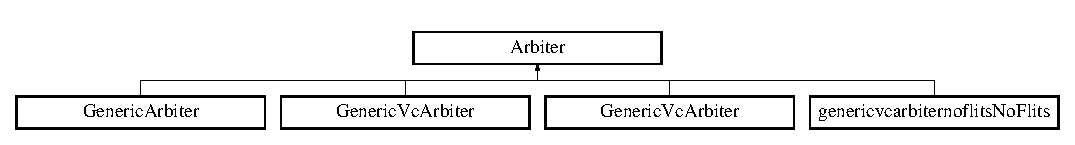
\includegraphics[height=1.50538cm]{classArbiter}
\end{center}
\end{figure}
\subsection*{Public Member Functions}
\begin{CompactItemize}
\item 
\hyperlink{classArbiter_ca96800fafab40183554debe9faf682d}{Arbiter} ()
\end{CompactItemize}


\subsection{Constructor \& Destructor Documentation}
\hypertarget{classArbiter_ca96800fafab40183554debe9faf682d}{
\index{Arbiter@{Arbiter}!Arbiter@{Arbiter}}
\index{Arbiter@{Arbiter}!Arbiter@{Arbiter}}
\subsubsection[{Arbiter}]{\setlength{\rightskip}{0pt plus 5cm}Arbiter::Arbiter ()\hspace{0.3cm}{\tt  \mbox{[}inline\mbox{]}}}}
\label{classArbiter_ca96800fafab40183554debe9faf682d}




The documentation for this class was generated from the following file:\begin{CompactItemize}
\item 
source/components/interfaces/\hyperlink{arbiter_8h}{arbiter.h}\end{CompactItemize}

\hypertarget{classBodyFlit}{
\section{BodyFlit Class Reference}
\label{classBodyFlit}\index{BodyFlit@{BodyFlit}}
}
{\tt \#include $<$flit.h$>$}

Inheritance diagram for BodyFlit::\begin{figure}[H]
\begin{center}
\leavevmode
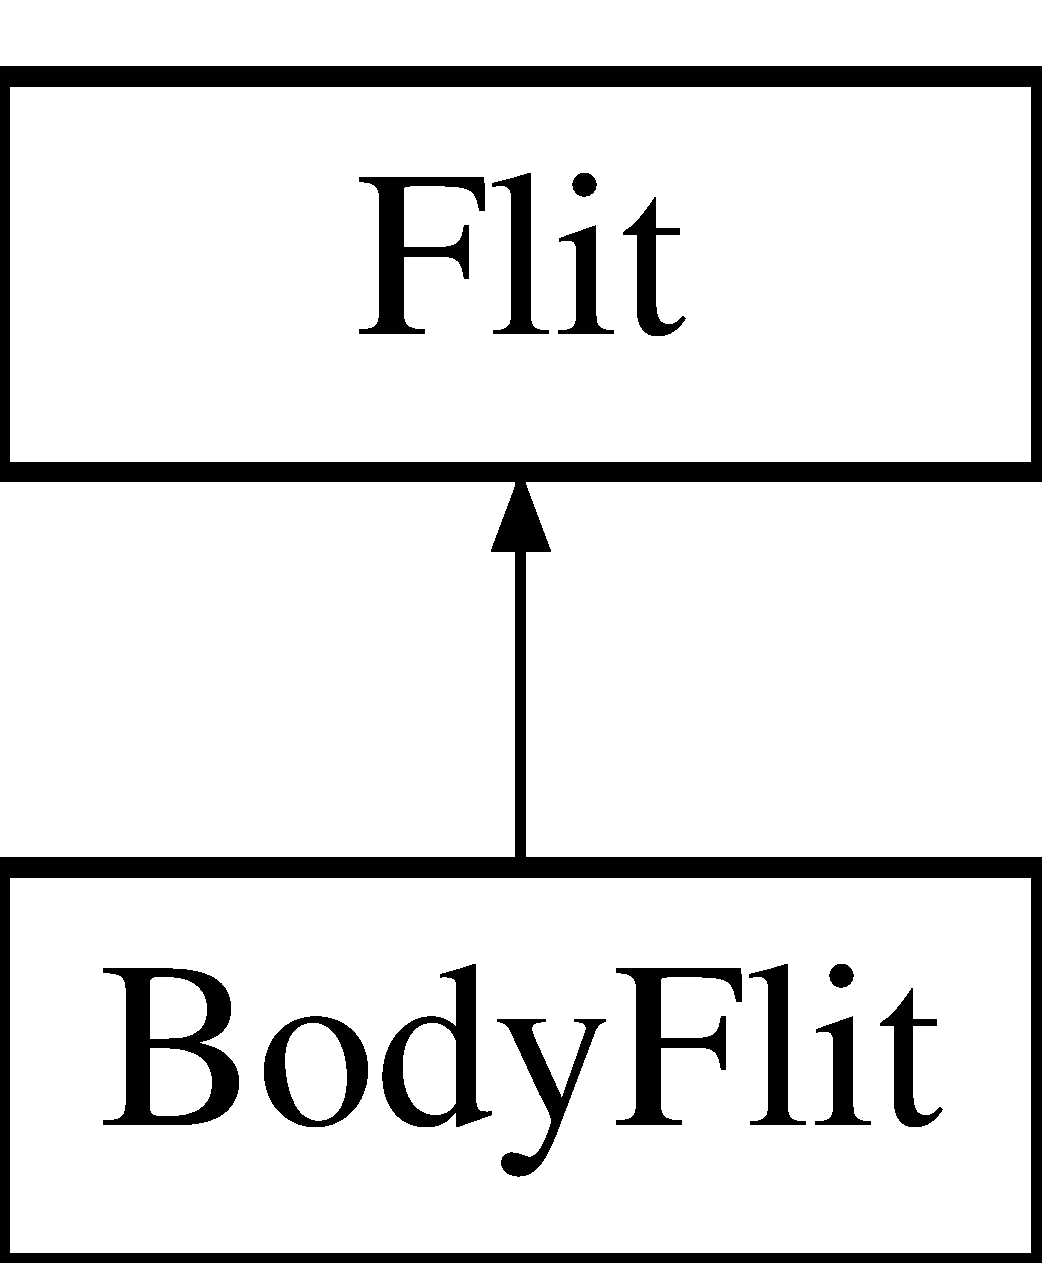
\includegraphics[height=2cm]{classBodyFlit}
\end{center}
\end{figure}
\subsection*{Public Member Functions}
\begin{CompactItemize}
\item 
\hyperlink{classBodyFlit_794842b7823df2d936bb652a34778d9b}{BodyFlit} ()
\item 
\hyperlink{classBodyFlit_52d1abfb160afc4146c978bd7b20fdaa}{$\sim$BodyFlit} ()
\item 
void \hyperlink{classBodyFlit_52eb491a5ee62a1f8f9ffc71d955da94}{populate\_\-body\_\-flit} (vector$<$ bool $>$ d)
\item 
std::string \hyperlink{classBodyFlit_408f02aae1a229c761ff0f3537675cde}{toString} () const 
\end{CompactItemize}


\subsection{Constructor \& Destructor Documentation}
\hypertarget{classBodyFlit_794842b7823df2d936bb652a34778d9b}{
\index{BodyFlit@{BodyFlit}!BodyFlit@{BodyFlit}}
\index{BodyFlit@{BodyFlit}!BodyFlit@{BodyFlit}}
\subsubsection[{BodyFlit}]{\setlength{\rightskip}{0pt plus 5cm}BodyFlit::BodyFlit ()}}
\label{classBodyFlit_794842b7823df2d936bb652a34778d9b}


\hypertarget{classBodyFlit_52d1abfb160afc4146c978bd7b20fdaa}{
\index{BodyFlit@{BodyFlit}!$\sim$BodyFlit@{$\sim$BodyFlit}}
\index{$\sim$BodyFlit@{$\sim$BodyFlit}!BodyFlit@{BodyFlit}}
\subsubsection[{$\sim$BodyFlit}]{\setlength{\rightskip}{0pt plus 5cm}BodyFlit::$\sim$BodyFlit ()}}
\label{classBodyFlit_52d1abfb160afc4146c978bd7b20fdaa}




\subsection{Member Function Documentation}
\hypertarget{classBodyFlit_52eb491a5ee62a1f8f9ffc71d955da94}{
\index{BodyFlit@{BodyFlit}!populate\_\-body\_\-flit@{populate\_\-body\_\-flit}}
\index{populate\_\-body\_\-flit@{populate\_\-body\_\-flit}!BodyFlit@{BodyFlit}}
\subsubsection[{populate\_\-body\_\-flit}]{\setlength{\rightskip}{0pt plus 5cm}void BodyFlit::populate\_\-body\_\-flit (vector$<$ bool $>$ {\em d})}}
\label{classBodyFlit_52eb491a5ee62a1f8f9ffc71d955da94}


\hypertarget{classBodyFlit_408f02aae1a229c761ff0f3537675cde}{
\index{BodyFlit@{BodyFlit}!toString@{toString}}
\index{toString@{toString}!BodyFlit@{BodyFlit}}
\subsubsection[{toString}]{\setlength{\rightskip}{0pt plus 5cm}string BodyFlit::toString () const}}
\label{classBodyFlit_408f02aae1a229c761ff0f3537675cde}




Reimplemented from \hyperlink{classFlit_ffc6c729a005389b51818aac59710dab}{Flit}.

The documentation for this class was generated from the following files:\begin{CompactItemize}
\item 
source/data\_\-types/impl/\hyperlink{flit_8h}{flit.h}\item 
source/data\_\-types/impl/\hyperlink{flit_8cc}{flit.cc}\end{CompactItemize}

\hypertarget{classBuffer}{
\section{Buffer Class Reference}
\label{classBuffer}\index{Buffer@{Buffer}}
}
{\tt \#include $<$buffer.h$>$}

Inheritance diagram for Buffer::\begin{figure}[H]
\begin{center}
\leavevmode
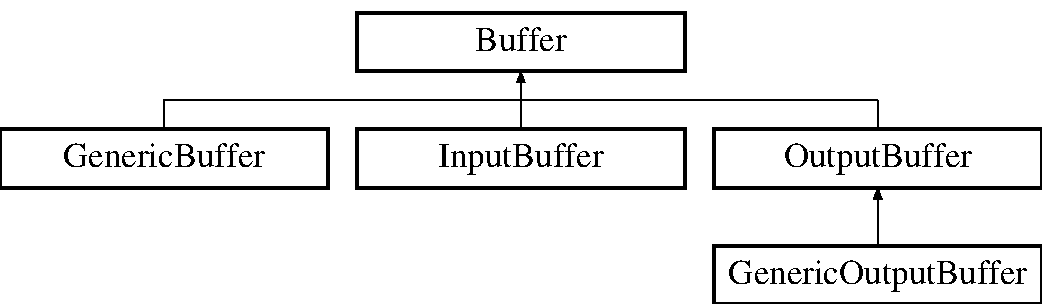
\includegraphics[height=3cm]{classBuffer}
\end{center}
\end{figure}
\subsection*{Public Member Functions}
\begin{CompactItemize}
\item 
\hyperlink{classBuffer_e7ef2cd201190fde551dcb902627112b}{Buffer} ()
\item 
\hyperlink{classBuffer_59b8743e4a5f731bdd0c4185c9ef263b}{$\sim$Buffer} ()
\item 
virtual void \hyperlink{classBuffer_c9dce1860c655146f000df30314caaa9}{push} (\hyperlink{classFlit}{Flit} $\ast$f)=0
\item 
virtual \hyperlink{classFlit}{Flit} $\ast$ \hyperlink{classBuffer_95f5c230f9c261bc13ddcfafcc340e7e}{pull} ()=0
\item 
virtual \hyperlink{outputBuffer_8h_91ad9478d81a7aaf2593e8d9c3d06a14}{uint} \hyperlink{classBuffer_af4e2d4031945429ae58350b5897570a}{get\_\-occupancy} (\hyperlink{outputBuffer_8h_91ad9478d81a7aaf2593e8d9c3d06a14}{uint} channel) const =0
\end{CompactItemize}


\subsection{Constructor \& Destructor Documentation}
\hypertarget{classBuffer_e7ef2cd201190fde551dcb902627112b}{
\index{Buffer@{Buffer}!Buffer@{Buffer}}
\index{Buffer@{Buffer}!Buffer@{Buffer}}
\subsubsection[{Buffer}]{\setlength{\rightskip}{0pt plus 5cm}Buffer::Buffer ()\hspace{0.3cm}{\tt  \mbox{[}inline\mbox{]}}}}
\label{classBuffer_e7ef2cd201190fde551dcb902627112b}


\hypertarget{classBuffer_59b8743e4a5f731bdd0c4185c9ef263b}{
\index{Buffer@{Buffer}!$\sim$Buffer@{$\sim$Buffer}}
\index{$\sim$Buffer@{$\sim$Buffer}!Buffer@{Buffer}}
\subsubsection[{$\sim$Buffer}]{\setlength{\rightskip}{0pt plus 5cm}Buffer::$\sim$Buffer ()\hspace{0.3cm}{\tt  \mbox{[}inline\mbox{]}}}}
\label{classBuffer_59b8743e4a5f731bdd0c4185c9ef263b}




\subsection{Member Function Documentation}
\hypertarget{classBuffer_af4e2d4031945429ae58350b5897570a}{
\index{Buffer@{Buffer}!get\_\-occupancy@{get\_\-occupancy}}
\index{get\_\-occupancy@{get\_\-occupancy}!Buffer@{Buffer}}
\subsubsection[{get\_\-occupancy}]{\setlength{\rightskip}{0pt plus 5cm}virtual {\bf uint} Buffer::get\_\-occupancy ({\bf uint} {\em channel}) const\hspace{0.3cm}{\tt  \mbox{[}pure virtual\mbox{]}}}}
\label{classBuffer_af4e2d4031945429ae58350b5897570a}




Implemented in \hyperlink{classGenericBuffer_f2f85cf979616bab9dad5373d25d7813}{GenericBuffer}, and \hyperlink{classGenericOutputBuffer_0b8b70b9b3ab71195eea8d0d810dce94}{GenericOutputBuffer}.\hypertarget{classBuffer_95f5c230f9c261bc13ddcfafcc340e7e}{
\index{Buffer@{Buffer}!pull@{pull}}
\index{pull@{pull}!Buffer@{Buffer}}
\subsubsection[{pull}]{\setlength{\rightskip}{0pt plus 5cm}virtual {\bf Flit}$\ast$ Buffer::pull ()\hspace{0.3cm}{\tt  \mbox{[}pure virtual\mbox{]}}}}
\label{classBuffer_95f5c230f9c261bc13ddcfafcc340e7e}




Implemented in \hyperlink{classGenericBuffer_6ce6f151eb6f65ec1fffafffb04a8f0e}{GenericBuffer}, and \hyperlink{classGenericOutputBuffer_3c3f1b425635f59b0539805945ddb1bd}{GenericOutputBuffer}.\hypertarget{classBuffer_c9dce1860c655146f000df30314caaa9}{
\index{Buffer@{Buffer}!push@{push}}
\index{push@{push}!Buffer@{Buffer}}
\subsubsection[{push}]{\setlength{\rightskip}{0pt plus 5cm}virtual void Buffer::push ({\bf Flit} $\ast$ {\em f})\hspace{0.3cm}{\tt  \mbox{[}pure virtual\mbox{]}}}}
\label{classBuffer_c9dce1860c655146f000df30314caaa9}




Implemented in \hyperlink{classGenericBuffer_c5a0781106485f9567898b49021f6346}{GenericBuffer}, and \hyperlink{classGenericOutputBuffer_f2b4047e054df5bb9b624ce0b0bbf0e2}{GenericOutputBuffer}.

The documentation for this class was generated from the following file:\begin{CompactItemize}
\item 
source/components/interfaces/\hyperlink{buffer_8h}{buffer.h}\end{CompactItemize}

\hypertarget{classClock}{
\section{Clock Class Reference}
\label{classClock}\index{Clock@{Clock}}
}
{\tt \#include $<$clock.h$>$}

\subsection*{Public Member Functions}
\begin{CompactItemize}
\item 
\hyperlink{classClock_dbc370eb6b5f8d01645cf440188160a8}{Clock} ()
\item 
void \hyperlink{classClock_5e9189774442cbafe557b6735fb91c6b}{updateTimestamp} ()
\end{CompactItemize}


\subsection{Constructor \& Destructor Documentation}
\hypertarget{classClock_dbc370eb6b5f8d01645cf440188160a8}{
\index{Clock@{Clock}!Clock@{Clock}}
\index{Clock@{Clock}!Clock@{Clock}}
\subsubsection[{Clock}]{\setlength{\rightskip}{0pt plus 5cm}Clock::Clock ()}}
\label{classClock_dbc370eb6b5f8d01645cf440188160a8}




\subsection{Member Function Documentation}
\hypertarget{classClock_5e9189774442cbafe557b6735fb91c6b}{
\index{Clock@{Clock}!updateTimestamp@{updateTimestamp}}
\index{updateTimestamp@{updateTimestamp}!Clock@{Clock}}
\subsubsection[{updateTimestamp}]{\setlength{\rightskip}{0pt plus 5cm}void Clock::updateTimestamp ()}}
\label{classClock_5e9189774442cbafe557b6735fb91c6b}




The documentation for this class was generated from the following files:\begin{CompactItemize}
\item 
source/tests/\hyperlink{clock_8h}{clock.h}\item 
source/tests/\hyperlink{clock_8cc}{clock.cc}\end{CompactItemize}

\hypertarget{classComponent}{
\section{Component Class Reference}
\label{classComponent}\index{Component@{Component}}
}
{\tt \#include $<$component.h$>$}

Inheritance diagram for Component::\begin{figure}[H]
\begin{center}
\leavevmode
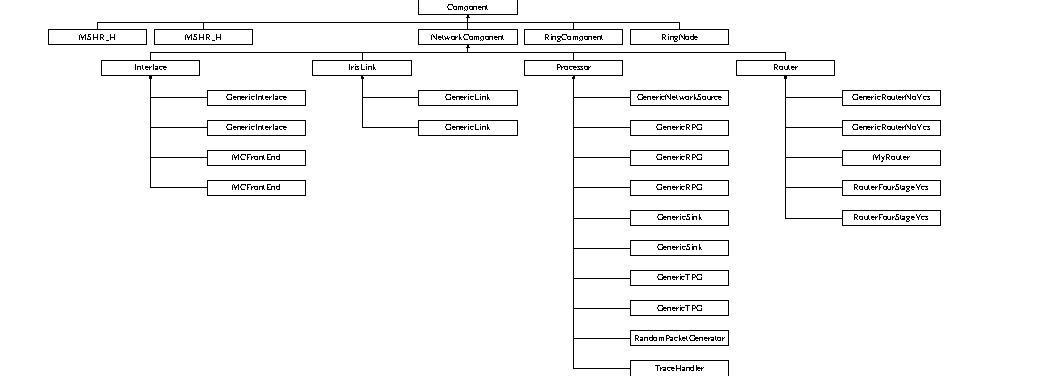
\includegraphics[height=5.05556cm]{classComponent}
\end{center}
\end{figure}
\subsection*{Public Member Functions}
\begin{CompactItemize}
\item 
\hyperlink{classComponent_8775db6d1a2c1afc2e77cd3c8f39da6f}{Component} ()
\item 
\hyperlink{classComponent_52f5a349d8ed4bd7efd4c8ee381a0ed8}{Component} (int lpId)
\item 
\hyperlink{classComponent_b8378fa275af98e568a7e91d33d867af}{$\sim$Component} ()
\item 
void \hyperlink{classComponent_4a5ca86f7a92e163287c4aae16f6b4b2}{setComponentId} (int id)
\item 
void \hyperlink{classComponent_9c7c91fe01f0d204cbc79b597d8236fe}{addInputLink} (\hyperlink{classLink}{Link} $\ast$l)
\item 
void \hyperlink{classComponent_aed97b38bbc44deddf329aa473e23b25}{addOutputLink} (\hyperlink{classLink}{Link} $\ast$l)
\item 
int \hyperlink{classComponent_af44955457bc84fa39a346ee70db916f}{myId} ()
\end{CompactItemize}
\subsection*{Public Attributes}
\begin{CompactItemize}
\item 
std::vector$<$ \hyperlink{classLink}{Link} $\ast$ $>$ \hyperlink{classComponent_6c43e56775c15cfcc1c0e8a6cbc7c474}{inLinks}
\item 
std::vector$<$ \hyperlink{classLink}{Link} $\ast$ $>$ \hyperlink{classComponent_4f715c718ecdb440f200e954b5d35b10}{outLinks}
\end{CompactItemize}


\subsection{Constructor \& Destructor Documentation}
\hypertarget{classComponent_8775db6d1a2c1afc2e77cd3c8f39da6f}{
\index{Component@{Component}!Component@{Component}}
\index{Component@{Component}!Component@{Component}}
\subsubsection[{Component}]{\setlength{\rightskip}{0pt plus 5cm}Component::Component ()}}
\label{classComponent_8775db6d1a2c1afc2e77cd3c8f39da6f}


\hypertarget{classComponent_52f5a349d8ed4bd7efd4c8ee381a0ed8}{
\index{Component@{Component}!Component@{Component}}
\index{Component@{Component}!Component@{Component}}
\subsubsection[{Component}]{\setlength{\rightskip}{0pt plus 5cm}Component::Component (int {\em lpId})}}
\label{classComponent_52f5a349d8ed4bd7efd4c8ee381a0ed8}


\hypertarget{classComponent_b8378fa275af98e568a7e91d33d867af}{
\index{Component@{Component}!$\sim$Component@{$\sim$Component}}
\index{$\sim$Component@{$\sim$Component}!Component@{Component}}
\subsubsection[{$\sim$Component}]{\setlength{\rightskip}{0pt plus 5cm}Component::$\sim$Component ()}}
\label{classComponent_b8378fa275af98e568a7e91d33d867af}




\subsection{Member Function Documentation}
\hypertarget{classComponent_9c7c91fe01f0d204cbc79b597d8236fe}{
\index{Component@{Component}!addInputLink@{addInputLink}}
\index{addInputLink@{addInputLink}!Component@{Component}}
\subsubsection[{addInputLink}]{\setlength{\rightskip}{0pt plus 5cm}void Component::addInputLink ({\bf Link} $\ast$ {\em l})}}
\label{classComponent_9c7c91fe01f0d204cbc79b597d8236fe}


\hypertarget{classComponent_aed97b38bbc44deddf329aa473e23b25}{
\index{Component@{Component}!addOutputLink@{addOutputLink}}
\index{addOutputLink@{addOutputLink}!Component@{Component}}
\subsubsection[{addOutputLink}]{\setlength{\rightskip}{0pt plus 5cm}void Component::addOutputLink ({\bf Link} $\ast$ {\em l})}}
\label{classComponent_aed97b38bbc44deddf329aa473e23b25}


\hypertarget{classComponent_af44955457bc84fa39a346ee70db916f}{
\index{Component@{Component}!myId@{myId}}
\index{myId@{myId}!Component@{Component}}
\subsubsection[{myId}]{\setlength{\rightskip}{0pt plus 5cm}int Component::myId ()\hspace{0.3cm}{\tt  \mbox{[}inline\mbox{]}}}}
\label{classComponent_af44955457bc84fa39a346ee70db916f}


\hypertarget{classComponent_4a5ca86f7a92e163287c4aae16f6b4b2}{
\index{Component@{Component}!setComponentId@{setComponentId}}
\index{setComponentId@{setComponentId}!Component@{Component}}
\subsubsection[{setComponentId}]{\setlength{\rightskip}{0pt plus 5cm}void Component::setComponentId (int {\em id})}}
\label{classComponent_4a5ca86f7a92e163287c4aae16f6b4b2}




\subsection{Member Data Documentation}
\hypertarget{classComponent_6c43e56775c15cfcc1c0e8a6cbc7c474}{
\index{Component@{Component}!inLinks@{inLinks}}
\index{inLinks@{inLinks}!Component@{Component}}
\subsubsection[{inLinks}]{\setlength{\rightskip}{0pt plus 5cm}std::vector$<${\bf Link}$\ast$$>$ {\bf Component::inLinks}}}
\label{classComponent_6c43e56775c15cfcc1c0e8a6cbc7c474}


\hypertarget{classComponent_4f715c718ecdb440f200e954b5d35b10}{
\index{Component@{Component}!outLinks@{outLinks}}
\index{outLinks@{outLinks}!Component@{Component}}
\subsubsection[{outLinks}]{\setlength{\rightskip}{0pt plus 5cm}std::vector$<${\bf Link}$\ast$$>$ {\bf Component::outLinks}}}
\label{classComponent_4f715c718ecdb440f200e954b5d35b10}




The documentation for this class was generated from the following files:\begin{CompactItemize}
\item 
source/kernel/\hyperlink{component_8h}{component.h}\item 
source/kernel/\hyperlink{component_8cc}{component.cc}\end{CompactItemize}

\hypertarget{classComponentDescription}{
\section{ComponentDescription Class Reference}
\label{classComponentDescription}\index{ComponentDescription@{ComponentDescription}}
}
{\tt \#include $<$simulator.h$>$}

\subsection*{Public Member Functions}
\begin{CompactItemize}
\item 
\hyperlink{classComponentDescription_ebcfce0c12f379fe3c7d19fc02a9751e}{ComponentDescription} (int lp, \hyperlink{classComponent}{Component} $\ast$obj)
\end{CompactItemize}
\subsection*{Public Attributes}
\begin{CompactItemize}
\item 
int \hyperlink{classComponentDescription_79464b7b6ee786c1396e33afa503292f}{lpId}
\item 
\hyperlink{classComponent}{Component} $\ast$ \hyperlink{classComponentDescription_784cd2019b9d92de3206075c48aefdea}{ptr}
\end{CompactItemize}


\subsection{Constructor \& Destructor Documentation}
\hypertarget{classComponentDescription_ebcfce0c12f379fe3c7d19fc02a9751e}{
\index{ComponentDescription@{ComponentDescription}!ComponentDescription@{ComponentDescription}}
\index{ComponentDescription@{ComponentDescription}!ComponentDescription@{ComponentDescription}}
\subsubsection[{ComponentDescription}]{\setlength{\rightskip}{0pt plus 5cm}ComponentDescription::ComponentDescription (int {\em lp}, \/  {\bf Component} $\ast$ {\em obj})\hspace{0.3cm}{\tt  \mbox{[}inline\mbox{]}}}}
\label{classComponentDescription_ebcfce0c12f379fe3c7d19fc02a9751e}




\subsection{Member Data Documentation}
\hypertarget{classComponentDescription_79464b7b6ee786c1396e33afa503292f}{
\index{ComponentDescription@{ComponentDescription}!lpId@{lpId}}
\index{lpId@{lpId}!ComponentDescription@{ComponentDescription}}
\subsubsection[{lpId}]{\setlength{\rightskip}{0pt plus 5cm}int {\bf ComponentDescription::lpId}}}
\label{classComponentDescription_79464b7b6ee786c1396e33afa503292f}


\hypertarget{classComponentDescription_784cd2019b9d92de3206075c48aefdea}{
\index{ComponentDescription@{ComponentDescription}!ptr@{ptr}}
\index{ptr@{ptr}!ComponentDescription@{ComponentDescription}}
\subsubsection[{ptr}]{\setlength{\rightskip}{0pt plus 5cm}{\bf Component}$\ast$ {\bf ComponentDescription::ptr}}}
\label{classComponentDescription_784cd2019b9d92de3206075c48aefdea}




The documentation for this class was generated from the following file:\begin{CompactItemize}
\item 
source/kernel/\hyperlink{simulator_8h}{simulator.h}\end{CompactItemize}

\hypertarget{classConstant}{
\section{Constant Class Reference}
\label{classConstant}\index{Constant@{Constant}}
}
{\tt \#include $<$rng.hpp$>$}

Inheritance diagram for Constant::\begin{figure}[H]
\begin{center}
\leavevmode
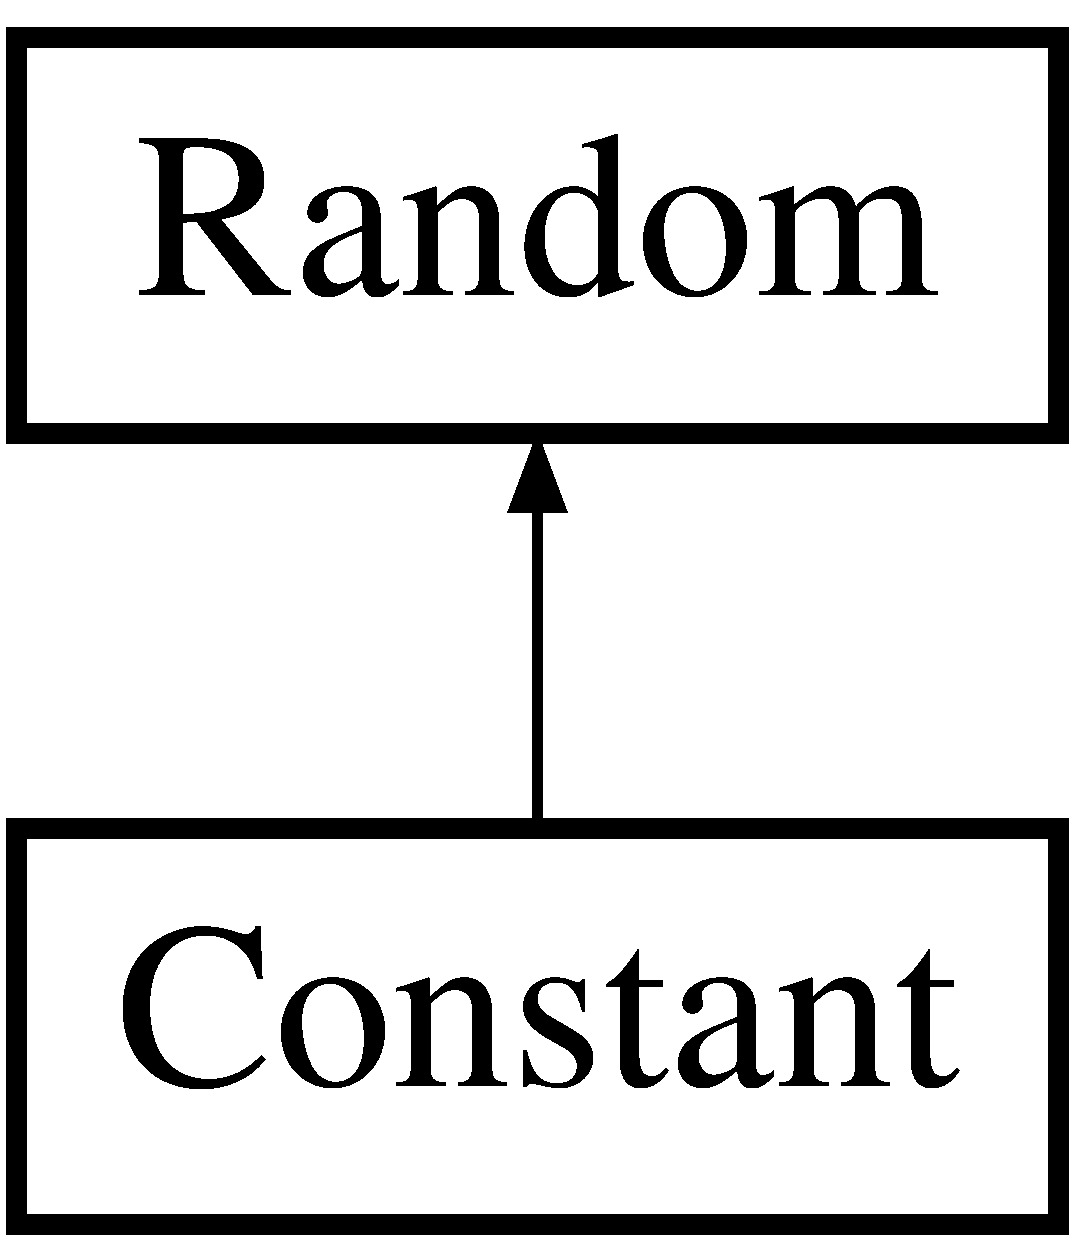
\includegraphics[height=2cm]{classConstant}
\end{center}
\end{figure}
\subsection*{Public Member Functions}
\begin{CompactItemize}
\item 
\hyperlink{classConstant_6d2f7d070d22aed4a3371c181da67716}{Constant} ()
\item 
\hyperlink{classConstant_df7e77573a679532a767f9557ed1745c}{Constant} (\hyperlink{rng_8hpp_ad41e7f5d86b1109b6a6a032c86cdd3f}{Random\_\-t} c)
\item 
\hyperlink{classConstant_0b4f8d8027a80d77b80ff8a186bd3c12}{Constant} (const \hyperlink{classConstant}{Constant} \&c)
\item 
void \hyperlink{classConstant_e5015bfe8179938344b0730e567929b0}{NewConstant} (\hyperlink{rng_8hpp_ad41e7f5d86b1109b6a6a032c86cdd3f}{Random\_\-t} c)
\item 
virtual \hyperlink{rng_8hpp_ad41e7f5d86b1109b6a6a032c86cdd3f}{Random\_\-t} \hyperlink{classConstant_8c4e39053835302870f15f5bbf0dc29e}{Value} ()
\item 
virtual \hyperlink{rng_8hpp_eb0f2eb55a063defa69eab89c6c0f695}{IRandom\_\-t} \hyperlink{classConstant_e7b431ef8fb785186bb846d23b5ccb95}{IntValue} ()
\item 
virtual \hyperlink{classRandom}{Random} $\ast$ \hyperlink{classConstant_47fc42d1d87bddf581084ae6b495ab2f}{Copy} () const 
\end{CompactItemize}


\subsection{Constructor \& Destructor Documentation}
\hypertarget{classConstant_6d2f7d070d22aed4a3371c181da67716}{
\index{Constant@{Constant}!Constant@{Constant}}
\index{Constant@{Constant}!Constant@{Constant}}
\subsubsection[{Constant}]{\setlength{\rightskip}{0pt plus 5cm}Constant::Constant ()\hspace{0.3cm}{\tt  \mbox{[}inline\mbox{]}}}}
\label{classConstant_6d2f7d070d22aed4a3371c181da67716}


\hypertarget{classConstant_df7e77573a679532a767f9557ed1745c}{
\index{Constant@{Constant}!Constant@{Constant}}
\index{Constant@{Constant}!Constant@{Constant}}
\subsubsection[{Constant}]{\setlength{\rightskip}{0pt plus 5cm}Constant::Constant ({\bf Random\_\-t} {\em c})\hspace{0.3cm}{\tt  \mbox{[}inline\mbox{]}}}}
\label{classConstant_df7e77573a679532a767f9557ed1745c}


\hypertarget{classConstant_0b4f8d8027a80d77b80ff8a186bd3c12}{
\index{Constant@{Constant}!Constant@{Constant}}
\index{Constant@{Constant}!Constant@{Constant}}
\subsubsection[{Constant}]{\setlength{\rightskip}{0pt plus 5cm}Constant::Constant (const {\bf Constant} \& {\em c})\hspace{0.3cm}{\tt  \mbox{[}inline\mbox{]}}}}
\label{classConstant_0b4f8d8027a80d77b80ff8a186bd3c12}




\subsection{Member Function Documentation}
\hypertarget{classConstant_47fc42d1d87bddf581084ae6b495ab2f}{
\index{Constant@{Constant}!Copy@{Copy}}
\index{Copy@{Copy}!Constant@{Constant}}
\subsubsection[{Copy}]{\setlength{\rightskip}{0pt plus 5cm}{\bf Random} $\ast$ Constant::Copy () const\hspace{0.3cm}{\tt  \mbox{[}virtual\mbox{]}}}}
\label{classConstant_47fc42d1d87bddf581084ae6b495ab2f}




Reimplemented from \hyperlink{classRandom_22b2951acd2008e8ff58fae434ab7ac5}{Random}.\hypertarget{classConstant_e7b431ef8fb785186bb846d23b5ccb95}{
\index{Constant@{Constant}!IntValue@{IntValue}}
\index{IntValue@{IntValue}!Constant@{Constant}}
\subsubsection[{IntValue}]{\setlength{\rightskip}{0pt plus 5cm}{\bf IRandom\_\-t} Constant::IntValue ()\hspace{0.3cm}{\tt  \mbox{[}virtual\mbox{]}}}}
\label{classConstant_e7b431ef8fb785186bb846d23b5ccb95}




Reimplemented from \hyperlink{classRandom_9ac522e9fe39aefd2cddd88554184b1a}{Random}.\hypertarget{classConstant_e5015bfe8179938344b0730e567929b0}{
\index{Constant@{Constant}!NewConstant@{NewConstant}}
\index{NewConstant@{NewConstant}!Constant@{Constant}}
\subsubsection[{NewConstant}]{\setlength{\rightskip}{0pt plus 5cm}void Constant::NewConstant ({\bf Random\_\-t} {\em c})\hspace{0.3cm}{\tt  \mbox{[}inline\mbox{]}}}}
\label{classConstant_e5015bfe8179938344b0730e567929b0}


\hypertarget{classConstant_8c4e39053835302870f15f5bbf0dc29e}{
\index{Constant@{Constant}!Value@{Value}}
\index{Value@{Value}!Constant@{Constant}}
\subsubsection[{Value}]{\setlength{\rightskip}{0pt plus 5cm}{\bf Random\_\-t} Constant::Value ()\hspace{0.3cm}{\tt  \mbox{[}virtual\mbox{]}}}}
\label{classConstant_8c4e39053835302870f15f5bbf0dc29e}




Reimplemented from \hyperlink{classRandom_4d1c2876c5c78104186e241209d0e11e}{Random}.

The documentation for this class was generated from the following files:\begin{CompactItemize}
\item 
source/randomNumbers/impl/\hyperlink{rng_8hpp}{rng.hpp}\item 
source/randomNumbers/impl/\hyperlink{rng_8cpp}{rng.cpp}\end{CompactItemize}

\hypertarget{classConstantSeed}{
\section{ConstantSeed Class Reference}
\label{classConstantSeed}\index{ConstantSeed@{ConstantSeed}}
}
{\tt \#include $<$rng.hpp$>$}

Inheritance diagram for ConstantSeed::\begin{figure}[H]
\begin{center}
\leavevmode
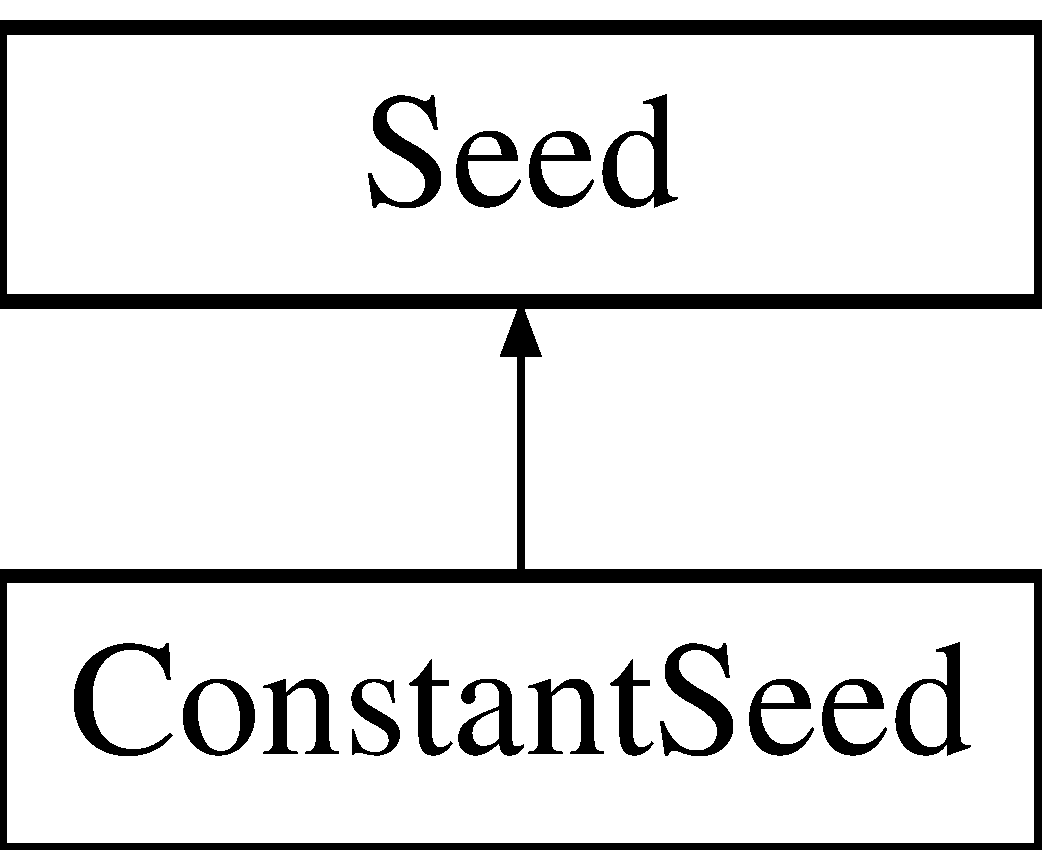
\includegraphics[height=2cm]{classConstantSeed}
\end{center}
\end{figure}
\subsection*{Public Member Functions}
\begin{CompactItemize}
\item 
\hyperlink{classConstantSeed_09dba071989c2d0d374c64c96cfdecc5}{ConstantSeed} (\hyperlink{rng_8hpp_d06dc1c21590adf4036ea4a265d06af8}{Seed\_\-t})
\item 
\hyperlink{classConstantSeed_b7706d24effc3222d0d284853d15b099}{ConstantSeed} (\hyperlink{rng_8hpp_d06dc1c21590adf4036ea4a265d06af8}{Seed\_\-t}, \hyperlink{rng_8hpp_d06dc1c21590adf4036ea4a265d06af8}{Seed\_\-t}, \hyperlink{rng_8hpp_d06dc1c21590adf4036ea4a265d06af8}{Seed\_\-t}, \hyperlink{rng_8hpp_d06dc1c21590adf4036ea4a265d06af8}{Seed\_\-t}, \hyperlink{rng_8hpp_d06dc1c21590adf4036ea4a265d06af8}{Seed\_\-t}, \hyperlink{rng_8hpp_d06dc1c21590adf4036ea4a265d06af8}{Seed\_\-t})
\item 
bool \hyperlink{classConstantSeed_38790f9390c6c4d6d27a2f60f1df438f}{IsRandom} () const 
\item 
\hyperlink{classConstantSeed_4c1bc70217c0522c76ebad617bd95f0d}{$\sim$ConstantSeed} ()
\end{CompactItemize}
\subsection*{Public Attributes}
\begin{CompactItemize}
\item 
\hyperlink{rng_8hpp_d06dc1c21590adf4036ea4a265d06af8}{Seed\_\-t} \hyperlink{classConstantSeed_10cdd2d1933e1af94162477edcad0352}{seeds} \mbox{[}6\mbox{]}
\end{CompactItemize}


\subsection{Constructor \& Destructor Documentation}
\hypertarget{classConstantSeed_09dba071989c2d0d374c64c96cfdecc5}{
\index{ConstantSeed@{ConstantSeed}!ConstantSeed@{ConstantSeed}}
\index{ConstantSeed@{ConstantSeed}!ConstantSeed@{ConstantSeed}}
\subsubsection[{ConstantSeed}]{\setlength{\rightskip}{0pt plus 5cm}ConstantSeed::ConstantSeed ({\bf Seed\_\-t} {\em s})}}
\label{classConstantSeed_09dba071989c2d0d374c64c96cfdecc5}


\hypertarget{classConstantSeed_b7706d24effc3222d0d284853d15b099}{
\index{ConstantSeed@{ConstantSeed}!ConstantSeed@{ConstantSeed}}
\index{ConstantSeed@{ConstantSeed}!ConstantSeed@{ConstantSeed}}
\subsubsection[{ConstantSeed}]{\setlength{\rightskip}{0pt plus 5cm}ConstantSeed::ConstantSeed ({\bf Seed\_\-t} {\em s0}, \/  {\bf Seed\_\-t} {\em s1}, \/  {\bf Seed\_\-t} {\em s2}, \/  {\bf Seed\_\-t} {\em s3}, \/  {\bf Seed\_\-t} {\em s4}, \/  {\bf Seed\_\-t} {\em s5})}}
\label{classConstantSeed_b7706d24effc3222d0d284853d15b099}


\hypertarget{classConstantSeed_4c1bc70217c0522c76ebad617bd95f0d}{
\index{ConstantSeed@{ConstantSeed}!$\sim$ConstantSeed@{$\sim$ConstantSeed}}
\index{$\sim$ConstantSeed@{$\sim$ConstantSeed}!ConstantSeed@{ConstantSeed}}
\subsubsection[{$\sim$ConstantSeed}]{\setlength{\rightskip}{0pt plus 5cm}ConstantSeed::$\sim$ConstantSeed ()\hspace{0.3cm}{\tt  \mbox{[}inline\mbox{]}}}}
\label{classConstantSeed_4c1bc70217c0522c76ebad617bd95f0d}




\subsection{Member Function Documentation}
\hypertarget{classConstantSeed_38790f9390c6c4d6d27a2f60f1df438f}{
\index{ConstantSeed@{ConstantSeed}!IsRandom@{IsRandom}}
\index{IsRandom@{IsRandom}!ConstantSeed@{ConstantSeed}}
\subsubsection[{IsRandom}]{\setlength{\rightskip}{0pt plus 5cm}bool ConstantSeed::IsRandom () const\hspace{0.3cm}{\tt  \mbox{[}inline, virtual\mbox{]}}}}
\label{classConstantSeed_38790f9390c6c4d6d27a2f60f1df438f}




Implements \hyperlink{classSeed_d07ddf0065c61a3dea72238a93e2bb35}{Seed}.

\subsection{Member Data Documentation}
\hypertarget{classConstantSeed_10cdd2d1933e1af94162477edcad0352}{
\index{ConstantSeed@{ConstantSeed}!seeds@{seeds}}
\index{seeds@{seeds}!ConstantSeed@{ConstantSeed}}
\subsubsection[{seeds}]{\setlength{\rightskip}{0pt plus 5cm}{\bf Seed\_\-t} {\bf ConstantSeed::seeds}\mbox{[}6\mbox{]}}}
\label{classConstantSeed_10cdd2d1933e1af94162477edcad0352}




The documentation for this class was generated from the following files:\begin{CompactItemize}
\item 
source/randomNumbers/impl/\hyperlink{rng_8hpp}{rng.hpp}\item 
source/randomNumbers/impl/\hyperlink{rng_8cpp}{rng.cpp}\end{CompactItemize}

\hypertarget{classCrossbar}{
\section{Crossbar Class Reference}
\label{classCrossbar}\index{Crossbar@{Crossbar}}
}
{\tt \#include $<$crossbar.h$>$}

Inheritance diagram for Crossbar::\begin{figure}[H]
\begin{center}
\leavevmode
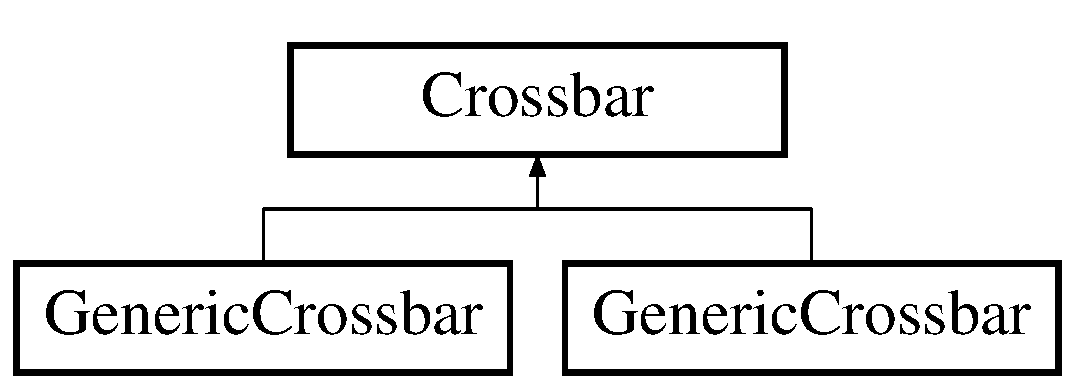
\includegraphics[height=2cm]{classCrossbar}
\end{center}
\end{figure}
\subsection*{Public Member Functions}
\begin{CompactItemize}
\item 
\hyperlink{classCrossbar_4093a8bf3894e372d4fa9ce06f2abf3d}{Crossbar} ()
\item 
virtual \hyperlink{classCrossbar_7debf5ed12155b31a21b13fff53357a6}{$\sim$Crossbar} ()
\item 
virtual void \hyperlink{classCrossbar_3223fa48d2c281d62747e4c10a14e1ba}{set\_\-input\_\-ports} (unsigned int ports)=0
\item 
virtual void \hyperlink{classCrossbar_291346aae5dfeee7ef946ee3addc3877}{set\_\-output\_\-ports} (unsigned int ports)=0
\item 
virtual unsigned int \hyperlink{classCrossbar_ec960231980043c3669add726b239e50}{get\_\-no\_\-input\_\-ports} ()=0
\item 
virtual unsigned int \hyperlink{classCrossbar_fa381d5e1af2576a2aaa5fb392072918}{get\_\-no\_\-output\_\-ports} ()=0
\item 
virtual void \hyperlink{classCrossbar_e7da6eea8ab565f26513dfe52d1516f5}{set\_\-no\_\-virtual\_\-channels} (unsigned int number)=0
\item 
virtual unsigned int \hyperlink{classCrossbar_a8e1c2a18960f4e6b9c076246239b092}{get\_\-no\_\-channels} ()=0
\item 
virtual unsigned int \hyperlink{classCrossbar_b7a6eee3263359c40f24dde01decfa20}{get\_\-map} (unsigned int input\_\-port, unsigned int channel)=0
\item 
virtual void \hyperlink{classCrossbar_8a7a059788ee336f171eb1d3c7be3110}{configure\_\-crossbar} (unsigned int input\_\-port, unsigned int output\_\-port, unsigned int channel)=0
\item 
virtual bool \hyperlink{classCrossbar_350fd72418bcb525209ae9e10c834468}{is\_\-full} (unsigned int input\_\-port, unsigned int channel)=0
\item 
virtual bool \hyperlink{classCrossbar_dc95dc76ac1c9f02a80ce7ada4559ce3}{is\_\-empty} (unsigned int output\_\-port, unsigned int channel)=0
\end{CompactItemize}


\subsection{Constructor \& Destructor Documentation}
\hypertarget{classCrossbar_4093a8bf3894e372d4fa9ce06f2abf3d}{
\index{Crossbar@{Crossbar}!Crossbar@{Crossbar}}
\index{Crossbar@{Crossbar}!Crossbar@{Crossbar}}
\subsubsection[{Crossbar}]{\setlength{\rightskip}{0pt plus 5cm}Crossbar::Crossbar ()\hspace{0.3cm}{\tt  \mbox{[}inline\mbox{]}}}}
\label{classCrossbar_4093a8bf3894e372d4fa9ce06f2abf3d}


\hypertarget{classCrossbar_7debf5ed12155b31a21b13fff53357a6}{
\index{Crossbar@{Crossbar}!$\sim$Crossbar@{$\sim$Crossbar}}
\index{$\sim$Crossbar@{$\sim$Crossbar}!Crossbar@{Crossbar}}
\subsubsection[{$\sim$Crossbar}]{\setlength{\rightskip}{0pt plus 5cm}virtual Crossbar::$\sim$Crossbar ()\hspace{0.3cm}{\tt  \mbox{[}inline, virtual\mbox{]}}}}
\label{classCrossbar_7debf5ed12155b31a21b13fff53357a6}




\subsection{Member Function Documentation}
\hypertarget{classCrossbar_8a7a059788ee336f171eb1d3c7be3110}{
\index{Crossbar@{Crossbar}!configure\_\-crossbar@{configure\_\-crossbar}}
\index{configure\_\-crossbar@{configure\_\-crossbar}!Crossbar@{Crossbar}}
\subsubsection[{configure\_\-crossbar}]{\setlength{\rightskip}{0pt plus 5cm}virtual void Crossbar::configure\_\-crossbar (unsigned int {\em input\_\-port}, \/  unsigned int {\em output\_\-port}, \/  unsigned int {\em channel})\hspace{0.3cm}{\tt  \mbox{[}pure virtual\mbox{]}}}}
\label{classCrossbar_8a7a059788ee336f171eb1d3c7be3110}




Implemented in \hyperlink{classGenericCrossbar_50c8203133960f74f6d82649b0c864be}{GenericCrossbar}, and \hyperlink{classGenericCrossbar_50c8203133960f74f6d82649b0c864be}{GenericCrossbar}.\hypertarget{classCrossbar_b7a6eee3263359c40f24dde01decfa20}{
\index{Crossbar@{Crossbar}!get\_\-map@{get\_\-map}}
\index{get\_\-map@{get\_\-map}!Crossbar@{Crossbar}}
\subsubsection[{get\_\-map}]{\setlength{\rightskip}{0pt plus 5cm}virtual unsigned int Crossbar::get\_\-map (unsigned int {\em input\_\-port}, \/  unsigned int {\em channel})\hspace{0.3cm}{\tt  \mbox{[}pure virtual\mbox{]}}}}
\label{classCrossbar_b7a6eee3263359c40f24dde01decfa20}




Implemented in \hyperlink{classGenericCrossbar_65b435392191561b7a4759e20aacab4e}{GenericCrossbar}, and \hyperlink{classGenericCrossbar_65b435392191561b7a4759e20aacab4e}{GenericCrossbar}.\hypertarget{classCrossbar_a8e1c2a18960f4e6b9c076246239b092}{
\index{Crossbar@{Crossbar}!get\_\-no\_\-channels@{get\_\-no\_\-channels}}
\index{get\_\-no\_\-channels@{get\_\-no\_\-channels}!Crossbar@{Crossbar}}
\subsubsection[{get\_\-no\_\-channels}]{\setlength{\rightskip}{0pt plus 5cm}virtual unsigned int Crossbar::get\_\-no\_\-channels ()\hspace{0.3cm}{\tt  \mbox{[}pure virtual\mbox{]}}}}
\label{classCrossbar_a8e1c2a18960f4e6b9c076246239b092}




Implemented in \hyperlink{classGenericCrossbar_945a3d32809787bd2c5ee68714467467}{GenericCrossbar}, and \hyperlink{classGenericCrossbar_945a3d32809787bd2c5ee68714467467}{GenericCrossbar}.\hypertarget{classCrossbar_ec960231980043c3669add726b239e50}{
\index{Crossbar@{Crossbar}!get\_\-no\_\-input\_\-ports@{get\_\-no\_\-input\_\-ports}}
\index{get\_\-no\_\-input\_\-ports@{get\_\-no\_\-input\_\-ports}!Crossbar@{Crossbar}}
\subsubsection[{get\_\-no\_\-input\_\-ports}]{\setlength{\rightskip}{0pt plus 5cm}virtual unsigned int Crossbar::get\_\-no\_\-input\_\-ports ()\hspace{0.3cm}{\tt  \mbox{[}pure virtual\mbox{]}}}}
\label{classCrossbar_ec960231980043c3669add726b239e50}




Implemented in \hyperlink{classGenericCrossbar_8758e38060de9899fa70ad069b83e9fc}{GenericCrossbar}, and \hyperlink{classGenericCrossbar_8758e38060de9899fa70ad069b83e9fc}{GenericCrossbar}.\hypertarget{classCrossbar_fa381d5e1af2576a2aaa5fb392072918}{
\index{Crossbar@{Crossbar}!get\_\-no\_\-output\_\-ports@{get\_\-no\_\-output\_\-ports}}
\index{get\_\-no\_\-output\_\-ports@{get\_\-no\_\-output\_\-ports}!Crossbar@{Crossbar}}
\subsubsection[{get\_\-no\_\-output\_\-ports}]{\setlength{\rightskip}{0pt plus 5cm}virtual unsigned int Crossbar::get\_\-no\_\-output\_\-ports ()\hspace{0.3cm}{\tt  \mbox{[}pure virtual\mbox{]}}}}
\label{classCrossbar_fa381d5e1af2576a2aaa5fb392072918}




Implemented in \hyperlink{classGenericCrossbar_6ca09eb5520228b39d718e3994a5b84f}{GenericCrossbar}, and \hyperlink{classGenericCrossbar_6ca09eb5520228b39d718e3994a5b84f}{GenericCrossbar}.\hypertarget{classCrossbar_dc95dc76ac1c9f02a80ce7ada4559ce3}{
\index{Crossbar@{Crossbar}!is\_\-empty@{is\_\-empty}}
\index{is\_\-empty@{is\_\-empty}!Crossbar@{Crossbar}}
\subsubsection[{is\_\-empty}]{\setlength{\rightskip}{0pt plus 5cm}virtual bool Crossbar::is\_\-empty (unsigned int {\em output\_\-port}, \/  unsigned int {\em channel})\hspace{0.3cm}{\tt  \mbox{[}pure virtual\mbox{]}}}}
\label{classCrossbar_dc95dc76ac1c9f02a80ce7ada4559ce3}




Implemented in \hyperlink{classGenericCrossbar_b1dc236c4543805ac9fd50f25adcc27e}{GenericCrossbar}, and \hyperlink{classGenericCrossbar_b1dc236c4543805ac9fd50f25adcc27e}{GenericCrossbar}.\hypertarget{classCrossbar_350fd72418bcb525209ae9e10c834468}{
\index{Crossbar@{Crossbar}!is\_\-full@{is\_\-full}}
\index{is\_\-full@{is\_\-full}!Crossbar@{Crossbar}}
\subsubsection[{is\_\-full}]{\setlength{\rightskip}{0pt plus 5cm}virtual bool Crossbar::is\_\-full (unsigned int {\em input\_\-port}, \/  unsigned int {\em channel})\hspace{0.3cm}{\tt  \mbox{[}pure virtual\mbox{]}}}}
\label{classCrossbar_350fd72418bcb525209ae9e10c834468}




Implemented in \hyperlink{classGenericCrossbar_1949b9db3b5b1950ad6a2c9e46103024}{GenericCrossbar}, and \hyperlink{classGenericCrossbar_1949b9db3b5b1950ad6a2c9e46103024}{GenericCrossbar}.\hypertarget{classCrossbar_3223fa48d2c281d62747e4c10a14e1ba}{
\index{Crossbar@{Crossbar}!set\_\-input\_\-ports@{set\_\-input\_\-ports}}
\index{set\_\-input\_\-ports@{set\_\-input\_\-ports}!Crossbar@{Crossbar}}
\subsubsection[{set\_\-input\_\-ports}]{\setlength{\rightskip}{0pt plus 5cm}virtual void Crossbar::set\_\-input\_\-ports (unsigned int {\em ports})\hspace{0.3cm}{\tt  \mbox{[}pure virtual\mbox{]}}}}
\label{classCrossbar_3223fa48d2c281d62747e4c10a14e1ba}




Implemented in \hyperlink{classGenericCrossbar_c97249405a9bc78f2c1c9c28ad660472}{GenericCrossbar}, and \hyperlink{classGenericCrossbar_c97249405a9bc78f2c1c9c28ad660472}{GenericCrossbar}.\hypertarget{classCrossbar_e7da6eea8ab565f26513dfe52d1516f5}{
\index{Crossbar@{Crossbar}!set\_\-no\_\-virtual\_\-channels@{set\_\-no\_\-virtual\_\-channels}}
\index{set\_\-no\_\-virtual\_\-channels@{set\_\-no\_\-virtual\_\-channels}!Crossbar@{Crossbar}}
\subsubsection[{set\_\-no\_\-virtual\_\-channels}]{\setlength{\rightskip}{0pt plus 5cm}virtual void Crossbar::set\_\-no\_\-virtual\_\-channels (unsigned int {\em number})\hspace{0.3cm}{\tt  \mbox{[}pure virtual\mbox{]}}}}
\label{classCrossbar_e7da6eea8ab565f26513dfe52d1516f5}




Implemented in \hyperlink{classGenericCrossbar_e9d67e36be87ea3169baa80ae52044e3}{GenericCrossbar}, and \hyperlink{classGenericCrossbar_e9d67e36be87ea3169baa80ae52044e3}{GenericCrossbar}.\hypertarget{classCrossbar_291346aae5dfeee7ef946ee3addc3877}{
\index{Crossbar@{Crossbar}!set\_\-output\_\-ports@{set\_\-output\_\-ports}}
\index{set\_\-output\_\-ports@{set\_\-output\_\-ports}!Crossbar@{Crossbar}}
\subsubsection[{set\_\-output\_\-ports}]{\setlength{\rightskip}{0pt plus 5cm}virtual void Crossbar::set\_\-output\_\-ports (unsigned int {\em ports})\hspace{0.3cm}{\tt  \mbox{[}pure virtual\mbox{]}}}}
\label{classCrossbar_291346aae5dfeee7ef946ee3addc3877}




Implemented in \hyperlink{classGenericCrossbar_5b9a2875ec8a1bb19683304ae31e3364}{GenericCrossbar}, and \hyperlink{classGenericCrossbar_5b9a2875ec8a1bb19683304ae31e3364}{GenericCrossbar}.

The documentation for this class was generated from the following file:\begin{CompactItemize}
\item 
source/components/interfaces/\hyperlink{crossbar_8h}{crossbar.h}\end{CompactItemize}

\hypertarget{structData}{
\section{Data Struct Reference}
\label{structData}\index{Data@{Data}}
}
{\tt \#include $<$request.h$>$}

\subsection*{Public Attributes}
\begin{CompactItemize}
\item 
unsigned long long int \hyperlink{structData_be8f049430369f7682bcee5a12072b4f}{value}
\item 
short \hyperlink{structData_3c66751e9b4f4968ad69df84c7922422}{size}
\end{CompactItemize}


\subsection{Member Data Documentation}
\hypertarget{structData_3c66751e9b4f4968ad69df84c7922422}{
\index{Data@{Data}!size@{size}}
\index{size@{size}!Data@{Data}}
\subsubsection[{size}]{\setlength{\rightskip}{0pt plus 5cm}short {\bf Data::size}}}
\label{structData_3c66751e9b4f4968ad69df84c7922422}


\hypertarget{structData_be8f049430369f7682bcee5a12072b4f}{
\index{Data@{Data}!value@{value}}
\index{value@{value}!Data@{Data}}
\subsubsection[{value}]{\setlength{\rightskip}{0pt plus 5cm}unsigned long long int {\bf Data::value}}}
\label{structData_be8f049430369f7682bcee5a12072b4f}




The documentation for this struct was generated from the following file:\begin{CompactItemize}
\item 
source/memctrl/\hyperlink{request_8h}{request.h}\end{CompactItemize}

\hypertarget{classDeterministic}{
\section{Deterministic Class Reference}
\label{classDeterministic}\index{Deterministic@{Deterministic}}
}
{\tt \#include $<$rng.hpp$>$}

Inheritance diagram for Deterministic::\begin{figure}[H]
\begin{center}
\leavevmode
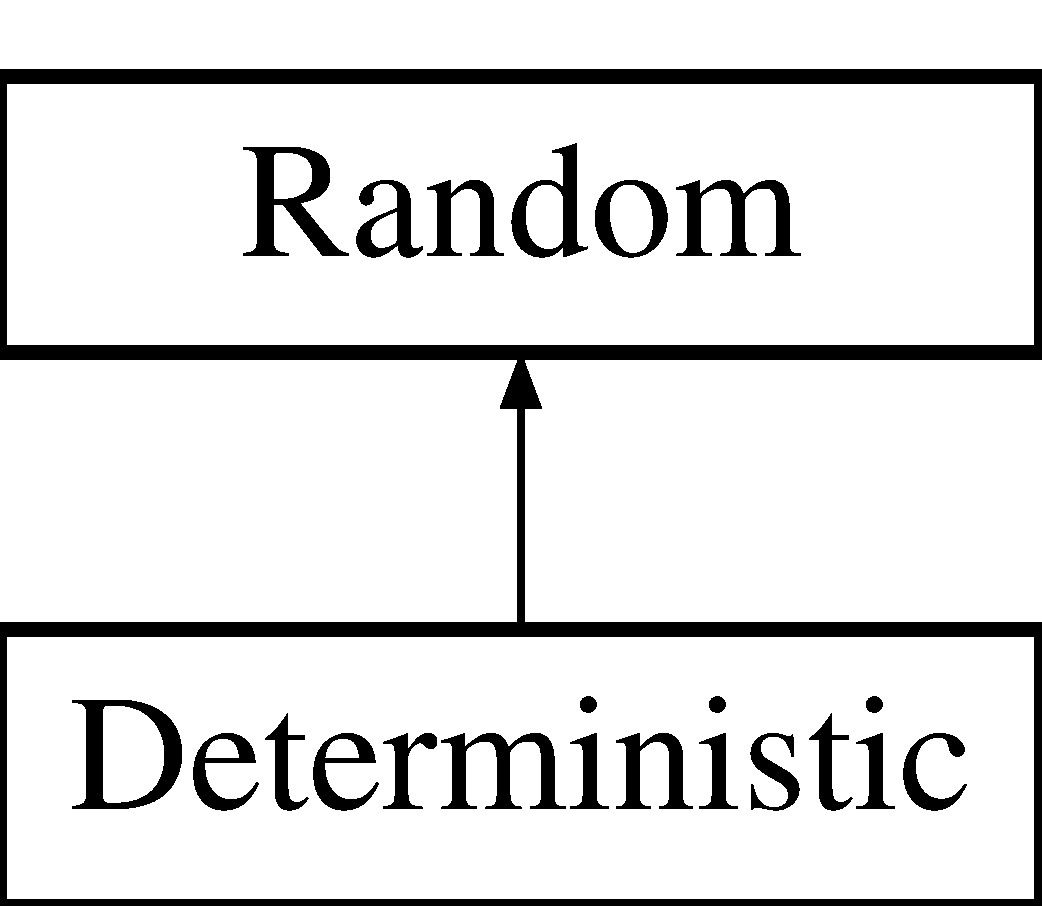
\includegraphics[height=2cm]{classDeterministic}
\end{center}
\end{figure}
\subsection*{Public Member Functions}
\begin{CompactItemize}
\item 
\hyperlink{classDeterministic_5012c74e6c4158a0d8dc1a5a9b625a98}{Deterministic} (\hyperlink{rng_8hpp_ad41e7f5d86b1109b6a6a032c86cdd3f}{Random\_\-t} $\ast$, \hyperlink{common-defs_8hpp_bdd4d02aefa61ef2e943e2c6a09566c6}{Count\_\-t})
\item 
virtual \hyperlink{classDeterministic_b14fdbe43ddacba07192a79b35bc76f7}{$\sim$Deterministic} ()
\item 
virtual \hyperlink{rng_8hpp_ad41e7f5d86b1109b6a6a032c86cdd3f}{Random\_\-t} \hyperlink{classDeterministic_5bca3d51cb08d3ec23579e09ce8e713f}{Value} ()
\item 
virtual \hyperlink{classRandom}{Random} $\ast$ \hyperlink{classDeterministic_4eb4260ecbc55661f1d9c268e6684ea4}{Copy} () const 
\end{CompactItemize}


\subsection{Constructor \& Destructor Documentation}
\hypertarget{classDeterministic_5012c74e6c4158a0d8dc1a5a9b625a98}{
\index{Deterministic@{Deterministic}!Deterministic@{Deterministic}}
\index{Deterministic@{Deterministic}!Deterministic@{Deterministic}}
\subsubsection[{Deterministic}]{\setlength{\rightskip}{0pt plus 5cm}Deterministic::Deterministic ({\bf Random\_\-t} $\ast$ {\em d}, \/  {\bf Count\_\-t} {\em c})\hspace{0.3cm}{\tt  \mbox{[}explicit\mbox{]}}}}
\label{classDeterministic_5012c74e6c4158a0d8dc1a5a9b625a98}


\hypertarget{classDeterministic_b14fdbe43ddacba07192a79b35bc76f7}{
\index{Deterministic@{Deterministic}!$\sim$Deterministic@{$\sim$Deterministic}}
\index{$\sim$Deterministic@{$\sim$Deterministic}!Deterministic@{Deterministic}}
\subsubsection[{$\sim$Deterministic}]{\setlength{\rightskip}{0pt plus 5cm}virtual Deterministic::$\sim$Deterministic ()\hspace{0.3cm}{\tt  \mbox{[}inline, virtual\mbox{]}}}}
\label{classDeterministic_b14fdbe43ddacba07192a79b35bc76f7}




\subsection{Member Function Documentation}
\hypertarget{classDeterministic_4eb4260ecbc55661f1d9c268e6684ea4}{
\index{Deterministic@{Deterministic}!Copy@{Copy}}
\index{Copy@{Copy}!Deterministic@{Deterministic}}
\subsubsection[{Copy}]{\setlength{\rightskip}{0pt plus 5cm}{\bf Random} $\ast$ Deterministic::Copy () const\hspace{0.3cm}{\tt  \mbox{[}virtual\mbox{]}}}}
\label{classDeterministic_4eb4260ecbc55661f1d9c268e6684ea4}




Reimplemented from \hyperlink{classRandom_22b2951acd2008e8ff58fae434ab7ac5}{Random}.\hypertarget{classDeterministic_5bca3d51cb08d3ec23579e09ce8e713f}{
\index{Deterministic@{Deterministic}!Value@{Value}}
\index{Value@{Value}!Deterministic@{Deterministic}}
\subsubsection[{Value}]{\setlength{\rightskip}{0pt plus 5cm}{\bf Random\_\-t} Deterministic::Value ()\hspace{0.3cm}{\tt  \mbox{[}virtual\mbox{]}}}}
\label{classDeterministic_5bca3d51cb08d3ec23579e09ce8e713f}




Reimplemented from \hyperlink{classRandom_4d1c2876c5c78104186e241209d0e11e}{Random}.

The documentation for this class was generated from the following files:\begin{CompactItemize}
\item 
source/randomNumbers/impl/\hyperlink{rng_8hpp}{rng.hpp}\item 
source/randomNumbers/impl/\hyperlink{rng_8cpp}{rng.cpp}\end{CompactItemize}

\hypertarget{classEmpirical}{
\section{Empirical Class Reference}
\label{classEmpirical}\index{Empirical@{Empirical}}
}
{\tt \#include $<$rng.hpp$>$}

Inheritance diagram for Empirical::\begin{figure}[H]
\begin{center}
\leavevmode
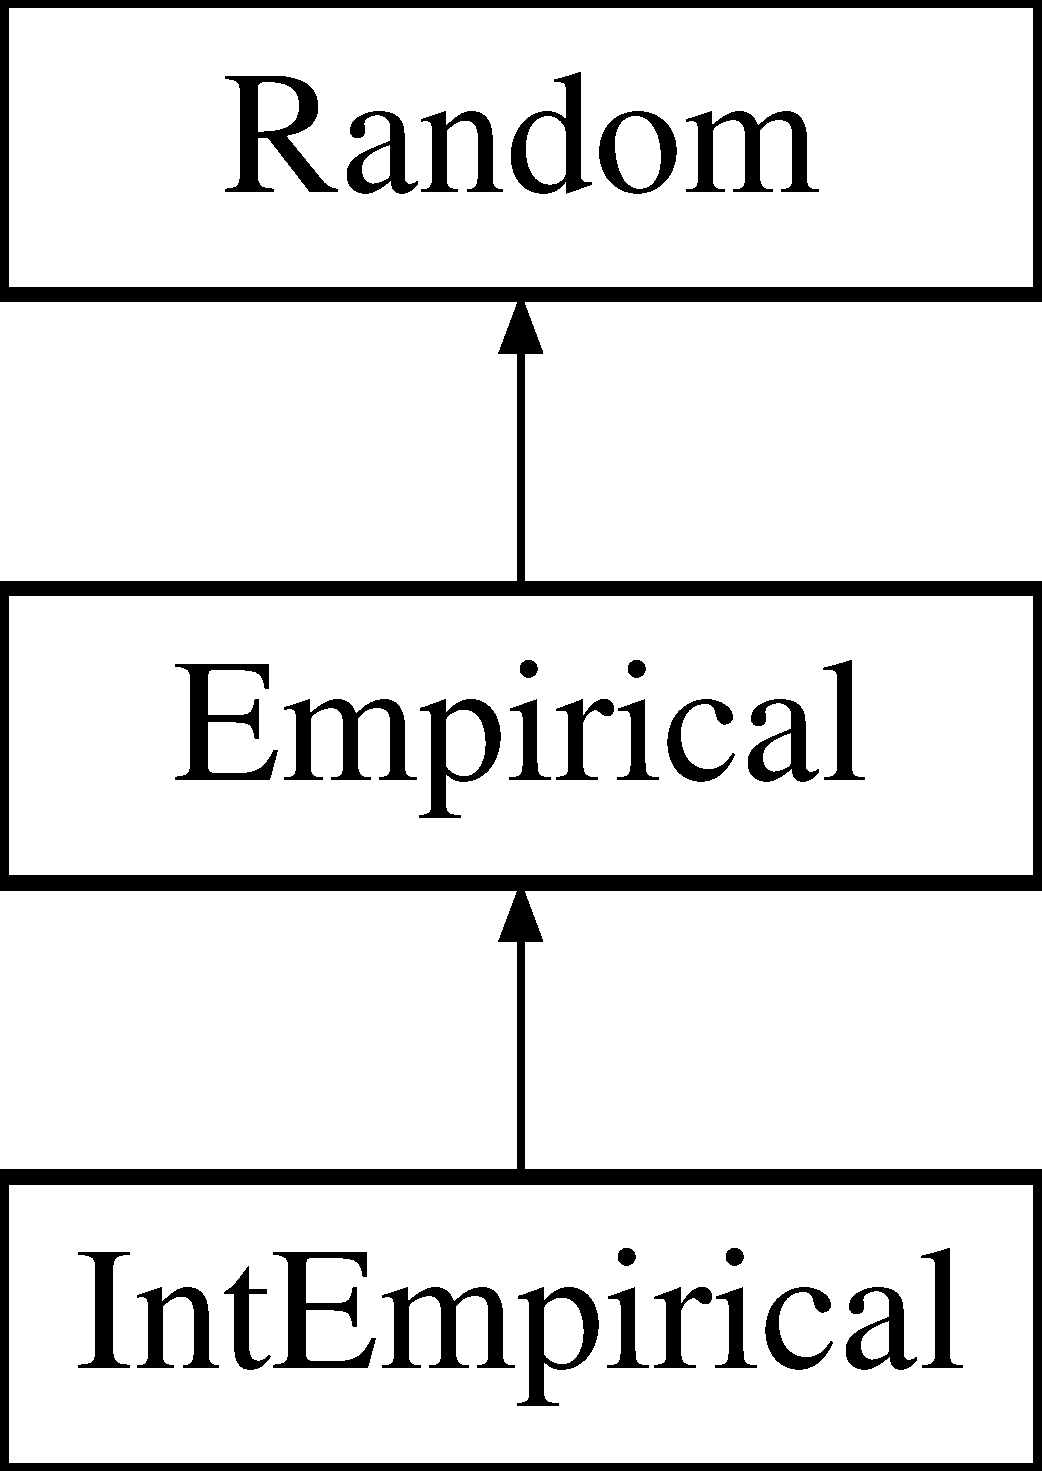
\includegraphics[height=3cm]{classEmpirical}
\end{center}
\end{figure}
\subsection*{Public Member Functions}
\begin{CompactItemize}
\item 
\hyperlink{classEmpirical_f2a9c05d8bac2f4698cb8f858b3a1724}{Empirical} ()
\item 
virtual \hyperlink{classEmpirical_d9422bac95c25865158cade0982516e4}{$\sim$Empirical} ()
\item 
\hyperlink{classEmpirical_c8e3a99d92dae74fe99ca47829821734}{Empirical} (const \hyperlink{classEmpirical}{Empirical} \&c)
\item 
virtual \hyperlink{rng_8hpp_ad41e7f5d86b1109b6a6a032c86cdd3f}{Random\_\-t} \hyperlink{classEmpirical_76b4c62b6fdcfbe2dbaff2462e4153ad}{Value} ()
\item 
virtual \hyperlink{classRandom}{Random} $\ast$ \hyperlink{classEmpirical_d5429fdf863d53d74649cc8c630cfb0b}{Copy} () const 
\item 
virtual void \hyperlink{classEmpirical_edc41dd73a4398ac77d537c78b9558de}{CDF} (\hyperlink{rng_8hpp_ad41e7f5d86b1109b6a6a032c86cdd3f}{Random\_\-t}, \hyperlink{rng_8hpp_68ff29d325e1cb493f27ede4fa99c8e4}{CDF\_\-t})
\end{CompactItemize}


\subsection{Constructor \& Destructor Documentation}
\hypertarget{classEmpirical_f2a9c05d8bac2f4698cb8f858b3a1724}{
\index{Empirical@{Empirical}!Empirical@{Empirical}}
\index{Empirical@{Empirical}!Empirical@{Empirical}}
\subsubsection[{Empirical}]{\setlength{\rightskip}{0pt plus 5cm}Empirical::Empirical ()\hspace{0.3cm}{\tt  \mbox{[}inline, explicit\mbox{]}}}}
\label{classEmpirical_f2a9c05d8bac2f4698cb8f858b3a1724}


\hypertarget{classEmpirical_d9422bac95c25865158cade0982516e4}{
\index{Empirical@{Empirical}!$\sim$Empirical@{$\sim$Empirical}}
\index{$\sim$Empirical@{$\sim$Empirical}!Empirical@{Empirical}}
\subsubsection[{$\sim$Empirical}]{\setlength{\rightskip}{0pt plus 5cm}virtual Empirical::$\sim$Empirical ()\hspace{0.3cm}{\tt  \mbox{[}inline, virtual\mbox{]}}}}
\label{classEmpirical_d9422bac95c25865158cade0982516e4}


\hypertarget{classEmpirical_c8e3a99d92dae74fe99ca47829821734}{
\index{Empirical@{Empirical}!Empirical@{Empirical}}
\index{Empirical@{Empirical}!Empirical@{Empirical}}
\subsubsection[{Empirical}]{\setlength{\rightskip}{0pt plus 5cm}Empirical::Empirical (const {\bf Empirical} \& {\em c})\hspace{0.3cm}{\tt  \mbox{[}inline\mbox{]}}}}
\label{classEmpirical_c8e3a99d92dae74fe99ca47829821734}




\subsection{Member Function Documentation}
\hypertarget{classEmpirical_edc41dd73a4398ac77d537c78b9558de}{
\index{Empirical@{Empirical}!CDF@{CDF}}
\index{CDF@{CDF}!Empirical@{Empirical}}
\subsubsection[{CDF}]{\setlength{\rightskip}{0pt plus 5cm}void Empirical::CDF ({\bf Random\_\-t} {\em v}, \/  {\bf CDF\_\-t} {\em c})\hspace{0.3cm}{\tt  \mbox{[}virtual\mbox{]}}}}
\label{classEmpirical_edc41dd73a4398ac77d537c78b9558de}


\hypertarget{classEmpirical_d5429fdf863d53d74649cc8c630cfb0b}{
\index{Empirical@{Empirical}!Copy@{Copy}}
\index{Copy@{Copy}!Empirical@{Empirical}}
\subsubsection[{Copy}]{\setlength{\rightskip}{0pt plus 5cm}{\bf Random} $\ast$ Empirical::Copy () const\hspace{0.3cm}{\tt  \mbox{[}virtual\mbox{]}}}}
\label{classEmpirical_d5429fdf863d53d74649cc8c630cfb0b}




Reimplemented from \hyperlink{classRandom_22b2951acd2008e8ff58fae434ab7ac5}{Random}.

Reimplemented in \hyperlink{classIntEmpirical_d7e809689f9158c050b8a386eb945636}{IntEmpirical}.\hypertarget{classEmpirical_76b4c62b6fdcfbe2dbaff2462e4153ad}{
\index{Empirical@{Empirical}!Value@{Value}}
\index{Value@{Value}!Empirical@{Empirical}}
\subsubsection[{Value}]{\setlength{\rightskip}{0pt plus 5cm}{\bf Random\_\-t} Empirical::Value ()\hspace{0.3cm}{\tt  \mbox{[}virtual\mbox{]}}}}
\label{classEmpirical_76b4c62b6fdcfbe2dbaff2462e4153ad}




Reimplemented from \hyperlink{classRandom_4d1c2876c5c78104186e241209d0e11e}{Random}.

The documentation for this class was generated from the following files:\begin{CompactItemize}
\item 
source/randomNumbers/impl/\hyperlink{rng_8hpp}{rng.hpp}\item 
source/randomNumbers/impl/\hyperlink{rng_8cpp}{rng.cpp}\end{CompactItemize}

\hypertarget{classEvent0}{
\section{Event0$<$ T, OBJ $>$ Class Template Reference}
\label{classEvent0}\index{Event0@{Event0}}
}
{\tt \#include $<$simulator.h$>$}

Inheritance diagram for Event0$<$ T, OBJ $>$::\begin{figure}[H]
\begin{center}
\leavevmode
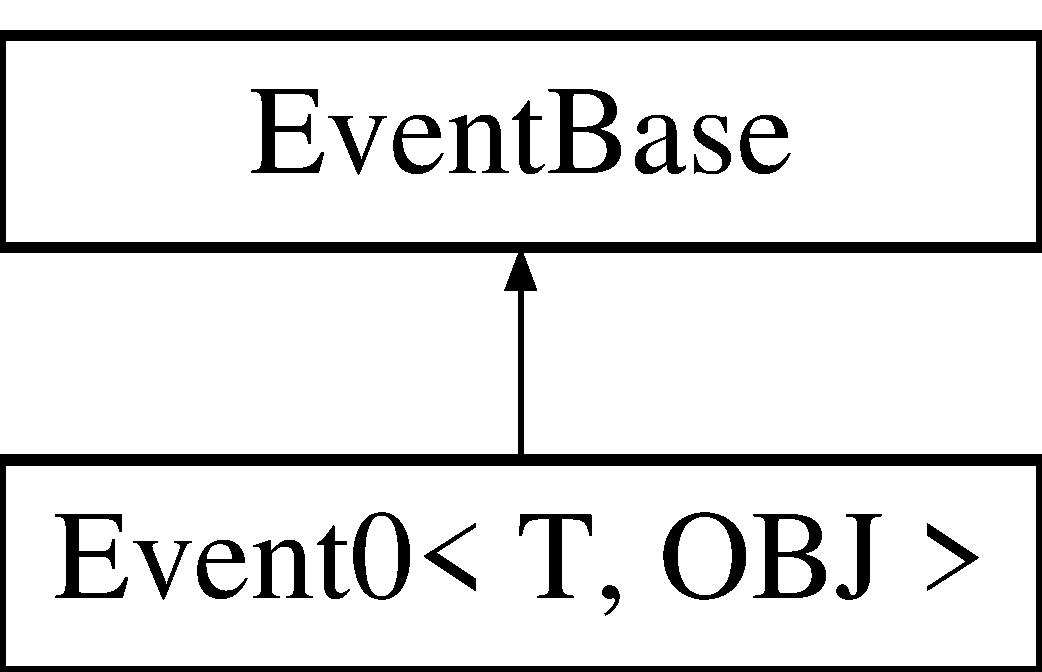
\includegraphics[height=2cm]{classEvent0}
\end{center}
\end{figure}
\subsection*{Public Member Functions}
\begin{CompactItemize}
\item 
\hyperlink{classEvent0_c3286a88ee0681958c96062c5325b48e}{Event0} (double t, void(T::$\ast$f)(void), OBJ $\ast$obj0)
\item 
void \hyperlink{classEvent0_77176d1040ed4cc48fa750c4854212b9}{CallHandler} ()
\end{CompactItemize}
\subsection*{Public Attributes}
\begin{CompactItemize}
\item 
void(T::$\ast$ \hyperlink{classEvent0_9f5c4b04f0f887ef7a2df146e10e9403}{handler} )(void)
\item 
OBJ $\ast$ \hyperlink{classEvent0_b37236e93d14993e36a8913ae2dbaf31}{obj}
\end{CompactItemize}
\subsubsection*{template$<$typename T, typename OBJ$>$ class Event0$<$ T, OBJ $>$}



\subsection{Constructor \& Destructor Documentation}
\hypertarget{classEvent0_c3286a88ee0681958c96062c5325b48e}{
\index{Event0@{Event0}!Event0@{Event0}}
\index{Event0@{Event0}!Event0@{Event0}}
\subsubsection[{Event0}]{\setlength{\rightskip}{0pt plus 5cm}template$<$typename T, typename OBJ$>$ {\bf Event0}$<$ T, OBJ $>$::{\bf Event0} (double {\em t}, \/  void(T::$\ast$)(void) {\em f}, \/  OBJ $\ast$ {\em obj0})\hspace{0.3cm}{\tt  \mbox{[}inline\mbox{]}}}}
\label{classEvent0_c3286a88ee0681958c96062c5325b48e}




\subsection{Member Function Documentation}
\hypertarget{classEvent0_77176d1040ed4cc48fa750c4854212b9}{
\index{Event0@{Event0}!CallHandler@{CallHandler}}
\index{CallHandler@{CallHandler}!Event0@{Event0}}
\subsubsection[{CallHandler}]{\setlength{\rightskip}{0pt plus 5cm}template$<$typename T , typename OBJ $>$ void {\bf Event0}$<$ T, OBJ $>$::CallHandler ()\hspace{0.3cm}{\tt  \mbox{[}inline, virtual\mbox{]}}}}
\label{classEvent0_77176d1040ed4cc48fa750c4854212b9}




Implements \hyperlink{classEventBase_121ca64dec88c8d9589c064b0060d037}{EventBase}.

\subsection{Member Data Documentation}
\hypertarget{classEvent0_9f5c4b04f0f887ef7a2df146e10e9403}{
\index{Event0@{Event0}!handler@{handler}}
\index{handler@{handler}!Event0@{Event0}}
\subsubsection[{handler}]{\setlength{\rightskip}{0pt plus 5cm}template$<$typename T, typename OBJ$>$ void(T::$\ast$ {\bf Event0}$<$ T, OBJ $>$::{\bf handler})(void)}}
\label{classEvent0_9f5c4b04f0f887ef7a2df146e10e9403}


\hypertarget{classEvent0_b37236e93d14993e36a8913ae2dbaf31}{
\index{Event0@{Event0}!obj@{obj}}
\index{obj@{obj}!Event0@{Event0}}
\subsubsection[{obj}]{\setlength{\rightskip}{0pt plus 5cm}template$<$typename T, typename OBJ$>$ OBJ$\ast$ {\bf Event0}$<$ T, OBJ $>$::{\bf obj}}}
\label{classEvent0_b37236e93d14993e36a8913ae2dbaf31}




The documentation for this class was generated from the following file:\begin{CompactItemize}
\item 
source/kernel/\hyperlink{simulator_8h}{simulator.h}\end{CompactItemize}

\hypertarget{classEvent0Stat}{
\section{Event0Stat Class Reference}
\label{classEvent0Stat}\index{Event0Stat@{Event0Stat}}
}
{\tt \#include $<$simulator.h$>$}

Inheritance diagram for Event0Stat::\begin{figure}[H]
\begin{center}
\leavevmode
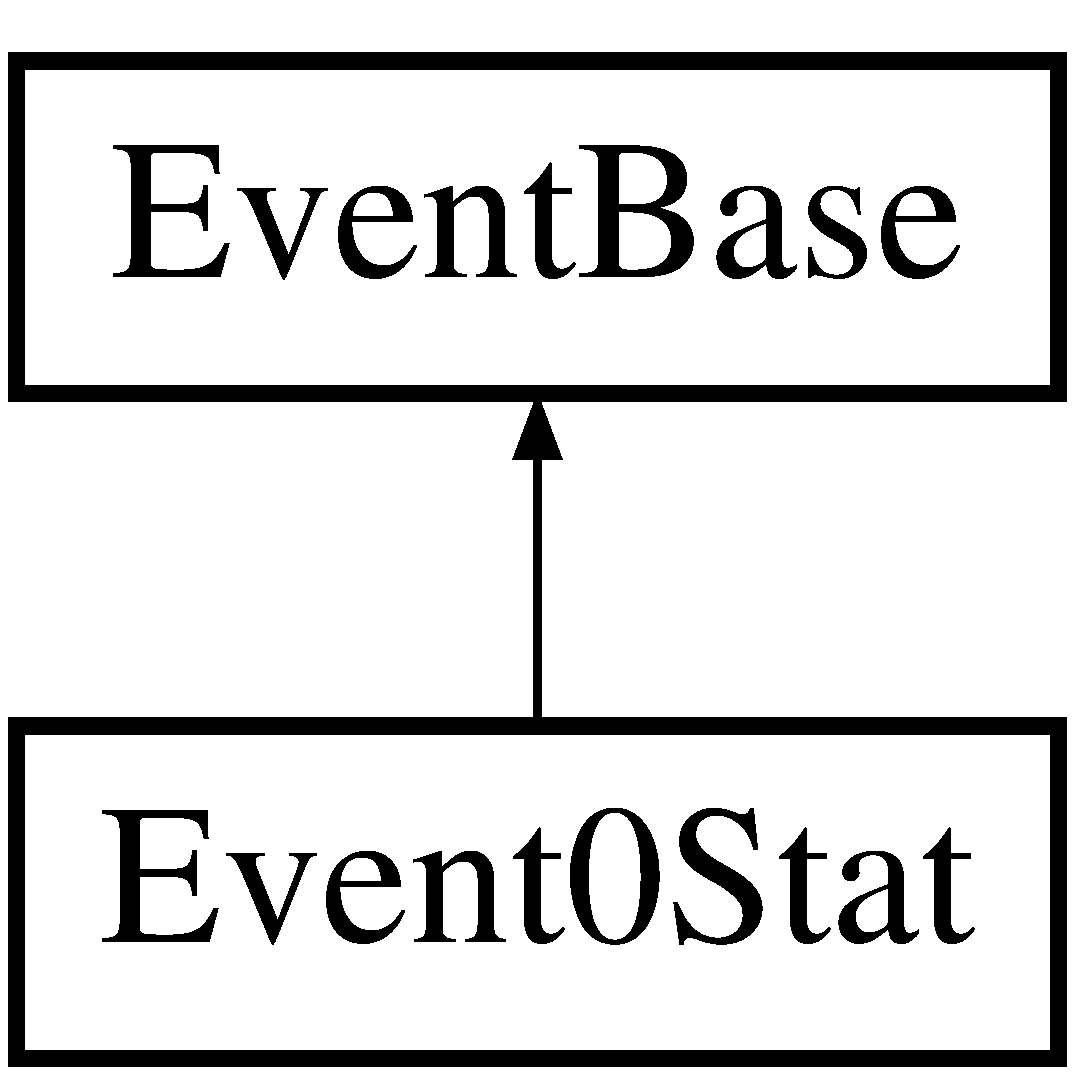
\includegraphics[height=2cm]{classEvent0Stat}
\end{center}
\end{figure}
\subsection*{Public Member Functions}
\begin{CompactItemize}
\item 
\hyperlink{classEvent0Stat_3d17a2a861561140b8d5cfdbfe359af4}{Event0Stat} (double t, void($\ast$f)(void))
\item 
void \hyperlink{classEvent0Stat_0cf3e0d44a1c04ee73a8a93a50ca05a1}{CallHandler} ()
\end{CompactItemize}
\subsection*{Public Attributes}
\begin{CompactItemize}
\item 
void($\ast$ \hyperlink{classEvent0Stat_6638fffbc4b497e2e8368d5e5f057db1}{handler} )(void)
\end{CompactItemize}


\subsection{Constructor \& Destructor Documentation}
\hypertarget{classEvent0Stat_3d17a2a861561140b8d5cfdbfe359af4}{
\index{Event0Stat@{Event0Stat}!Event0Stat@{Event0Stat}}
\index{Event0Stat@{Event0Stat}!Event0Stat@{Event0Stat}}
\subsubsection[{Event0Stat}]{\setlength{\rightskip}{0pt plus 5cm}Event0Stat::Event0Stat (double {\em t}, \/  void($\ast$)(void) {\em f})\hspace{0.3cm}{\tt  \mbox{[}inline\mbox{]}}}}
\label{classEvent0Stat_3d17a2a861561140b8d5cfdbfe359af4}




\subsection{Member Function Documentation}
\hypertarget{classEvent0Stat_0cf3e0d44a1c04ee73a8a93a50ca05a1}{
\index{Event0Stat@{Event0Stat}!CallHandler@{CallHandler}}
\index{CallHandler@{CallHandler}!Event0Stat@{Event0Stat}}
\subsubsection[{CallHandler}]{\setlength{\rightskip}{0pt plus 5cm}void Event0Stat::CallHandler ()\hspace{0.3cm}{\tt  \mbox{[}virtual\mbox{]}}}}
\label{classEvent0Stat_0cf3e0d44a1c04ee73a8a93a50ca05a1}




Implements \hyperlink{classEventBase_121ca64dec88c8d9589c064b0060d037}{EventBase}.

\subsection{Member Data Documentation}
\hypertarget{classEvent0Stat_6638fffbc4b497e2e8368d5e5f057db1}{
\index{Event0Stat@{Event0Stat}!handler@{handler}}
\index{handler@{handler}!Event0Stat@{Event0Stat}}
\subsubsection[{handler}]{\setlength{\rightskip}{0pt plus 5cm}void($\ast$ {\bf Event0Stat::handler})(void)}}
\label{classEvent0Stat_6638fffbc4b497e2e8368d5e5f057db1}




The documentation for this class was generated from the following files:\begin{CompactItemize}
\item 
source/kernel/\hyperlink{simulator_8h}{simulator.h}\item 
source/kernel/\hyperlink{simulator_8cc}{simulator.cc}\end{CompactItemize}

\hypertarget{classEvent1}{
\section{Event1$<$ T, OBJ, U1, T1 $>$ Class Template Reference}
\label{classEvent1}\index{Event1@{Event1}}
}
{\tt \#include $<$simulator.h$>$}

Inheritance diagram for Event1$<$ T, OBJ, U1, T1 $>$::\begin{figure}[H]
\begin{center}
\leavevmode
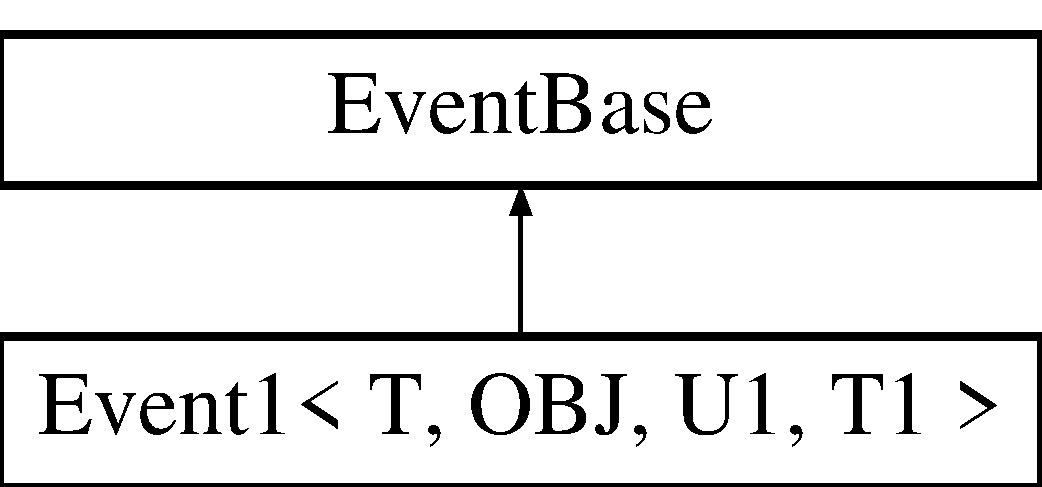
\includegraphics[height=2cm]{classEvent1}
\end{center}
\end{figure}
\subsection*{Public Member Functions}
\begin{CompactItemize}
\item 
\hyperlink{classEvent1_e53edac1393d2f7920f936ba6c7f90ba}{Event1} (double t, void(T::$\ast$f)(U1), OBJ $\ast$obj0, T1 t1\_\-0)
\item 
void \hyperlink{classEvent1_6d7e716e16ab6ee6672807250860cdd8}{CallHandler} ()
\end{CompactItemize}
\subsection*{Public Attributes}
\begin{CompactItemize}
\item 
void(T::$\ast$ \hyperlink{classEvent1_2a02ab5cbd37a2879c3db25cf3faf80f}{handler} )(U1)
\item 
OBJ $\ast$ \hyperlink{classEvent1_dc793df07c00b32a012cf45b31b9d2e6}{obj}
\item 
T1 \hyperlink{classEvent1_1af2759e05940a423f3b9409feab75f9}{t1}
\end{CompactItemize}
\subsubsection*{template$<$typename T, typename OBJ, typename U1, typename T1$>$ class Event1$<$ T, OBJ, U1, T1 $>$}



\subsection{Constructor \& Destructor Documentation}
\hypertarget{classEvent1_e53edac1393d2f7920f936ba6c7f90ba}{
\index{Event1@{Event1}!Event1@{Event1}}
\index{Event1@{Event1}!Event1@{Event1}}
\subsubsection[{Event1}]{\setlength{\rightskip}{0pt plus 5cm}template$<$typename T, typename OBJ, typename U1, typename T1$>$ {\bf Event1}$<$ T, OBJ, U1, T1 $>$::{\bf Event1} (double {\em t}, \/  void(T::$\ast$)(U1) {\em f}, \/  OBJ $\ast$ {\em obj0}, \/  T1 {\em t1\_\-0})\hspace{0.3cm}{\tt  \mbox{[}inline\mbox{]}}}}
\label{classEvent1_e53edac1393d2f7920f936ba6c7f90ba}




\subsection{Member Function Documentation}
\hypertarget{classEvent1_6d7e716e16ab6ee6672807250860cdd8}{
\index{Event1@{Event1}!CallHandler@{CallHandler}}
\index{CallHandler@{CallHandler}!Event1@{Event1}}
\subsubsection[{CallHandler}]{\setlength{\rightskip}{0pt plus 5cm}template$<$typename T , typename OBJ , typename U1 , typename T1 $>$ void {\bf Event1}$<$ T, OBJ, U1, T1 $>$::CallHandler ()\hspace{0.3cm}{\tt  \mbox{[}inline, virtual\mbox{]}}}}
\label{classEvent1_6d7e716e16ab6ee6672807250860cdd8}




Implements \hyperlink{classEventBase_121ca64dec88c8d9589c064b0060d037}{EventBase}.

\subsection{Member Data Documentation}
\hypertarget{classEvent1_2a02ab5cbd37a2879c3db25cf3faf80f}{
\index{Event1@{Event1}!handler@{handler}}
\index{handler@{handler}!Event1@{Event1}}
\subsubsection[{handler}]{\setlength{\rightskip}{0pt plus 5cm}template$<$typename T, typename OBJ, typename U1, typename T1$>$ void(T::$\ast$ {\bf Event1}$<$ T, OBJ, U1, T1 $>$::{\bf handler})(U1)}}
\label{classEvent1_2a02ab5cbd37a2879c3db25cf3faf80f}


\hypertarget{classEvent1_dc793df07c00b32a012cf45b31b9d2e6}{
\index{Event1@{Event1}!obj@{obj}}
\index{obj@{obj}!Event1@{Event1}}
\subsubsection[{obj}]{\setlength{\rightskip}{0pt plus 5cm}template$<$typename T, typename OBJ, typename U1, typename T1$>$ OBJ$\ast$ {\bf Event1}$<$ T, OBJ, U1, T1 $>$::{\bf obj}}}
\label{classEvent1_dc793df07c00b32a012cf45b31b9d2e6}


\hypertarget{classEvent1_1af2759e05940a423f3b9409feab75f9}{
\index{Event1@{Event1}!t1@{t1}}
\index{t1@{t1}!Event1@{Event1}}
\subsubsection[{t1}]{\setlength{\rightskip}{0pt plus 5cm}template$<$typename T, typename OBJ, typename U1, typename T1$>$ T1 {\bf Event1}$<$ T, OBJ, U1, T1 $>$::{\bf t1}}}
\label{classEvent1_1af2759e05940a423f3b9409feab75f9}




The documentation for this class was generated from the following file:\begin{CompactItemize}
\item 
source/kernel/\hyperlink{simulator_8h}{simulator.h}\end{CompactItemize}

\hypertarget{classEvent1Stat}{
\section{Event1Stat$<$ U1, T1 $>$ Class Template Reference}
\label{classEvent1Stat}\index{Event1Stat@{Event1Stat}}
}
{\tt \#include $<$simulator.h$>$}

Inheritance diagram for Event1Stat$<$ U1, T1 $>$::\begin{figure}[H]
\begin{center}
\leavevmode
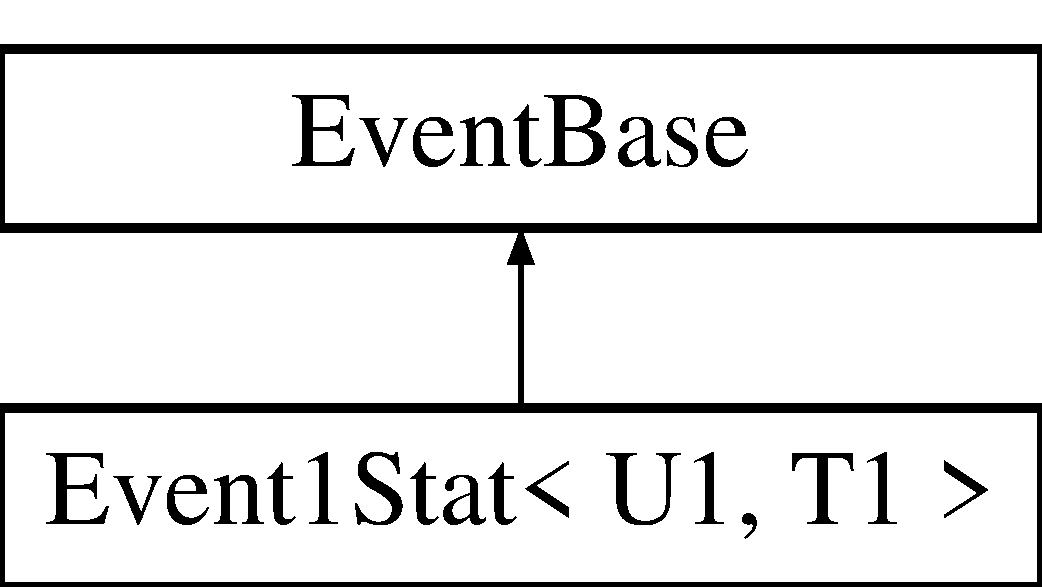
\includegraphics[height=2cm]{classEvent1Stat}
\end{center}
\end{figure}
\subsection*{Public Member Functions}
\begin{CompactItemize}
\item 
\hyperlink{classEvent1Stat_18fbb4bda5eec5c76b184c1905e6a51b}{Event1Stat} (double t, void($\ast$f)(U1), T1 t1\_\-0)
\item 
void \hyperlink{classEvent1Stat_d39942fb840e55ee829decdf1927eadf}{CallHandler} ()
\end{CompactItemize}
\subsection*{Public Attributes}
\begin{CompactItemize}
\item 
void($\ast$ \hyperlink{classEvent1Stat_d5c1915ba5261468e90f35d2e4200af7}{handler} )(U1)
\item 
T1 \hyperlink{classEvent1Stat_d8c7245671d807e6ffe5fefb08a1345c}{t1}
\end{CompactItemize}
\subsubsection*{template$<$typename U1, typename T1$>$ class Event1Stat$<$ U1, T1 $>$}



\subsection{Constructor \& Destructor Documentation}
\hypertarget{classEvent1Stat_18fbb4bda5eec5c76b184c1905e6a51b}{
\index{Event1Stat@{Event1Stat}!Event1Stat@{Event1Stat}}
\index{Event1Stat@{Event1Stat}!Event1Stat@{Event1Stat}}
\subsubsection[{Event1Stat}]{\setlength{\rightskip}{0pt plus 5cm}template$<$typename U1, typename T1$>$ {\bf Event1Stat}$<$ U1, T1 $>$::{\bf Event1Stat} (double {\em t}, \/  void($\ast$)(U1) {\em f}, \/  T1 {\em t1\_\-0})\hspace{0.3cm}{\tt  \mbox{[}inline\mbox{]}}}}
\label{classEvent1Stat_18fbb4bda5eec5c76b184c1905e6a51b}




\subsection{Member Function Documentation}
\hypertarget{classEvent1Stat_d39942fb840e55ee829decdf1927eadf}{
\index{Event1Stat@{Event1Stat}!CallHandler@{CallHandler}}
\index{CallHandler@{CallHandler}!Event1Stat@{Event1Stat}}
\subsubsection[{CallHandler}]{\setlength{\rightskip}{0pt plus 5cm}template$<$typename U1 , typename T1 $>$ void {\bf Event1Stat}$<$ U1, T1 $>$::CallHandler ()\hspace{0.3cm}{\tt  \mbox{[}inline, virtual\mbox{]}}}}
\label{classEvent1Stat_d39942fb840e55ee829decdf1927eadf}




Implements \hyperlink{classEventBase_121ca64dec88c8d9589c064b0060d037}{EventBase}.

\subsection{Member Data Documentation}
\hypertarget{classEvent1Stat_d5c1915ba5261468e90f35d2e4200af7}{
\index{Event1Stat@{Event1Stat}!handler@{handler}}
\index{handler@{handler}!Event1Stat@{Event1Stat}}
\subsubsection[{handler}]{\setlength{\rightskip}{0pt plus 5cm}template$<$typename U1, typename T1$>$ void($\ast$ {\bf Event1Stat}$<$ U1, T1 $>$::{\bf handler})(U1)}}
\label{classEvent1Stat_d5c1915ba5261468e90f35d2e4200af7}


\hypertarget{classEvent1Stat_d8c7245671d807e6ffe5fefb08a1345c}{
\index{Event1Stat@{Event1Stat}!t1@{t1}}
\index{t1@{t1}!Event1Stat@{Event1Stat}}
\subsubsection[{t1}]{\setlength{\rightskip}{0pt plus 5cm}template$<$typename U1, typename T1$>$ T1 {\bf Event1Stat}$<$ U1, T1 $>$::{\bf t1}}}
\label{classEvent1Stat_d8c7245671d807e6ffe5fefb08a1345c}




The documentation for this class was generated from the following file:\begin{CompactItemize}
\item 
source/kernel/\hyperlink{simulator_8h}{simulator.h}\end{CompactItemize}

\hypertarget{classEvent2}{
\section{Event2$<$ T, OBJ, U1, T1, U2, T2 $>$ Class Template Reference}
\label{classEvent2}\index{Event2@{Event2}}
}
{\tt \#include $<$simulator.h$>$}

Inheritance diagram for Event2$<$ T, OBJ, U1, T1, U2, T2 $>$::\begin{figure}[H]
\begin{center}
\leavevmode
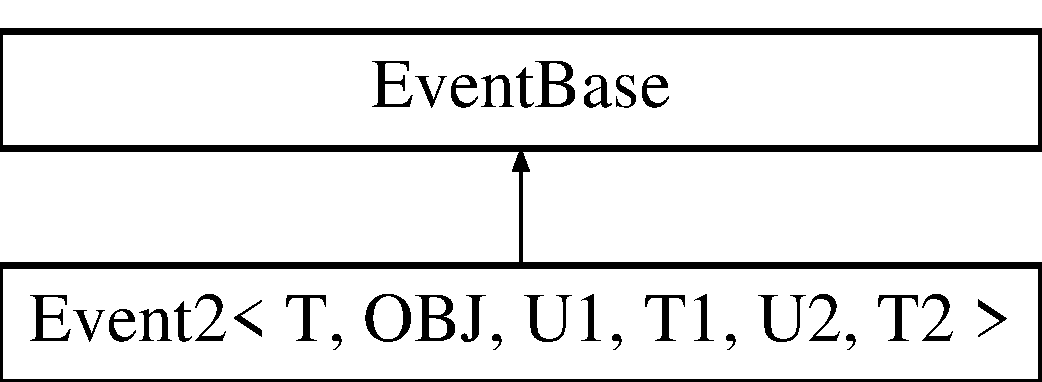
\includegraphics[height=2cm]{classEvent2}
\end{center}
\end{figure}
\subsection*{Public Member Functions}
\begin{CompactItemize}
\item 
\hyperlink{classEvent2_ba7c624909641184917f7a5603ab2ebe}{Event2} (double t, void(T::$\ast$f)(U1, U2), OBJ $\ast$obj0, T1 t1\_\-0, T2 t2\_\-0)
\item 
void \hyperlink{classEvent2_428b314837eee680fa435cad61944af3}{CallHandler} ()
\end{CompactItemize}
\subsection*{Public Attributes}
\begin{CompactItemize}
\item 
void(T::$\ast$ \hyperlink{classEvent2_166c37cb53b2969dac38fa79b0349768}{handler} )(U1, U2)
\item 
OBJ $\ast$ \hyperlink{classEvent2_e87200a757f09d76ae6aa5abd293f062}{obj}
\item 
T1 \hyperlink{classEvent2_b3e9b3c8ae4bff79e765e54a4947f371}{t1}
\item 
T2 \hyperlink{classEvent2_d921b4a0baa31fa2400fd022bf3b43e9}{t2}
\end{CompactItemize}
\subsubsection*{template$<$typename T, typename OBJ, typename U1, typename T1, typename U2, typename T2$>$ class Event2$<$ T, OBJ, U1, T1, U2, T2 $>$}



\subsection{Constructor \& Destructor Documentation}
\hypertarget{classEvent2_ba7c624909641184917f7a5603ab2ebe}{
\index{Event2@{Event2}!Event2@{Event2}}
\index{Event2@{Event2}!Event2@{Event2}}
\subsubsection[{Event2}]{\setlength{\rightskip}{0pt plus 5cm}template$<$typename T, typename OBJ, typename U1, typename T1, typename U2, typename T2$>$ {\bf Event2}$<$ T, OBJ, U1, T1, U2, T2 $>$::{\bf Event2} (double {\em t}, \/  void(T::$\ast$)(U1, U2) {\em f}, \/  OBJ $\ast$ {\em obj0}, \/  T1 {\em t1\_\-0}, \/  T2 {\em t2\_\-0})\hspace{0.3cm}{\tt  \mbox{[}inline\mbox{]}}}}
\label{classEvent2_ba7c624909641184917f7a5603ab2ebe}




\subsection{Member Function Documentation}
\hypertarget{classEvent2_428b314837eee680fa435cad61944af3}{
\index{Event2@{Event2}!CallHandler@{CallHandler}}
\index{CallHandler@{CallHandler}!Event2@{Event2}}
\subsubsection[{CallHandler}]{\setlength{\rightskip}{0pt plus 5cm}template$<$typename T , typename OBJ , typename U1 , typename T1 , typename U2 , typename T2 $>$ void {\bf Event2}$<$ T, OBJ, U1, T1, U2, T2 $>$::CallHandler ()\hspace{0.3cm}{\tt  \mbox{[}inline, virtual\mbox{]}}}}
\label{classEvent2_428b314837eee680fa435cad61944af3}




Implements \hyperlink{classEventBase_121ca64dec88c8d9589c064b0060d037}{EventBase}.

\subsection{Member Data Documentation}
\hypertarget{classEvent2_166c37cb53b2969dac38fa79b0349768}{
\index{Event2@{Event2}!handler@{handler}}
\index{handler@{handler}!Event2@{Event2}}
\subsubsection[{handler}]{\setlength{\rightskip}{0pt plus 5cm}template$<$typename T, typename OBJ, typename U1, typename T1, typename U2, typename T2$>$ void(T::$\ast$ {\bf Event2}$<$ T, OBJ, U1, T1, U2, T2 $>$::{\bf handler})(U1, U2)}}
\label{classEvent2_166c37cb53b2969dac38fa79b0349768}


\hypertarget{classEvent2_e87200a757f09d76ae6aa5abd293f062}{
\index{Event2@{Event2}!obj@{obj}}
\index{obj@{obj}!Event2@{Event2}}
\subsubsection[{obj}]{\setlength{\rightskip}{0pt plus 5cm}template$<$typename T, typename OBJ, typename U1, typename T1, typename U2, typename T2$>$ OBJ$\ast$ {\bf Event2}$<$ T, OBJ, U1, T1, U2, T2 $>$::{\bf obj}}}
\label{classEvent2_e87200a757f09d76ae6aa5abd293f062}


\hypertarget{classEvent2_b3e9b3c8ae4bff79e765e54a4947f371}{
\index{Event2@{Event2}!t1@{t1}}
\index{t1@{t1}!Event2@{Event2}}
\subsubsection[{t1}]{\setlength{\rightskip}{0pt plus 5cm}template$<$typename T, typename OBJ, typename U1, typename T1, typename U2, typename T2$>$ T1 {\bf Event2}$<$ T, OBJ, U1, T1, U2, T2 $>$::{\bf t1}}}
\label{classEvent2_b3e9b3c8ae4bff79e765e54a4947f371}


\hypertarget{classEvent2_d921b4a0baa31fa2400fd022bf3b43e9}{
\index{Event2@{Event2}!t2@{t2}}
\index{t2@{t2}!Event2@{Event2}}
\subsubsection[{t2}]{\setlength{\rightskip}{0pt plus 5cm}template$<$typename T, typename OBJ, typename U1, typename T1, typename U2, typename T2$>$ T2 {\bf Event2}$<$ T, OBJ, U1, T1, U2, T2 $>$::{\bf t2}}}
\label{classEvent2_d921b4a0baa31fa2400fd022bf3b43e9}




The documentation for this class was generated from the following file:\begin{CompactItemize}
\item 
source/kernel/\hyperlink{simulator_8h}{simulator.h}\end{CompactItemize}

\hypertarget{classEvent2Stat}{
\section{Event2Stat$<$ U1, T1, U2, T2 $>$ Class Template Reference}
\label{classEvent2Stat}\index{Event2Stat@{Event2Stat}}
}
{\tt \#include $<$simulator.h$>$}

Inheritance diagram for Event2Stat$<$ U1, T1, U2, T2 $>$::\begin{figure}[H]
\begin{center}
\leavevmode
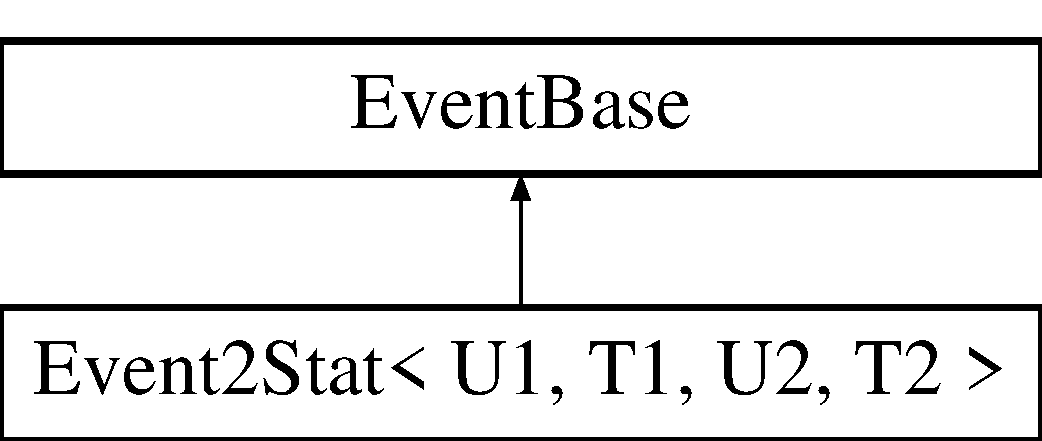
\includegraphics[height=2cm]{classEvent2Stat}
\end{center}
\end{figure}
\subsection*{Public Member Functions}
\begin{CompactItemize}
\item 
\hyperlink{classEvent2Stat_ad167681d8833e8300e76e60d8766b81}{Event2Stat} (double t, void($\ast$f)(U1, U2), T1 t1\_\-0, T2 t2\_\-0)
\item 
void \hyperlink{classEvent2Stat_84e6e9e412678507da3b2bde8e6a157a}{CallHandler} ()
\end{CompactItemize}
\subsection*{Public Attributes}
\begin{CompactItemize}
\item 
void($\ast$ \hyperlink{classEvent2Stat_c376cfc98a16f3365e21be171d8d491a}{handler} )(U1, U2)
\item 
T1 \hyperlink{classEvent2Stat_5daf0d729d5a79162abdb89b4efb19c1}{t1}
\item 
T2 \hyperlink{classEvent2Stat_ebb30c7ef2db2fb567415879c49827fb}{t2}
\end{CompactItemize}
\subsubsection*{template$<$typename U1, typename T1, typename U2, typename T2$>$ class Event2Stat$<$ U1, T1, U2, T2 $>$}



\subsection{Constructor \& Destructor Documentation}
\hypertarget{classEvent2Stat_ad167681d8833e8300e76e60d8766b81}{
\index{Event2Stat@{Event2Stat}!Event2Stat@{Event2Stat}}
\index{Event2Stat@{Event2Stat}!Event2Stat@{Event2Stat}}
\subsubsection[{Event2Stat}]{\setlength{\rightskip}{0pt plus 5cm}template$<$typename U1, typename T1, typename U2, typename T2$>$ {\bf Event2Stat}$<$ U1, T1, U2, T2 $>$::{\bf Event2Stat} (double {\em t}, \/  void($\ast$)(U1, U2) {\em f}, \/  T1 {\em t1\_\-0}, \/  T2 {\em t2\_\-0})\hspace{0.3cm}{\tt  \mbox{[}inline\mbox{]}}}}
\label{classEvent2Stat_ad167681d8833e8300e76e60d8766b81}




\subsection{Member Function Documentation}
\hypertarget{classEvent2Stat_84e6e9e412678507da3b2bde8e6a157a}{
\index{Event2Stat@{Event2Stat}!CallHandler@{CallHandler}}
\index{CallHandler@{CallHandler}!Event2Stat@{Event2Stat}}
\subsubsection[{CallHandler}]{\setlength{\rightskip}{0pt plus 5cm}template$<$typename U1 , typename T1 , typename U2 , typename T2 $>$ void {\bf Event2Stat}$<$ U1, T1, U2, T2 $>$::CallHandler ()\hspace{0.3cm}{\tt  \mbox{[}inline, virtual\mbox{]}}}}
\label{classEvent2Stat_84e6e9e412678507da3b2bde8e6a157a}




Implements \hyperlink{classEventBase_121ca64dec88c8d9589c064b0060d037}{EventBase}.

\subsection{Member Data Documentation}
\hypertarget{classEvent2Stat_c376cfc98a16f3365e21be171d8d491a}{
\index{Event2Stat@{Event2Stat}!handler@{handler}}
\index{handler@{handler}!Event2Stat@{Event2Stat}}
\subsubsection[{handler}]{\setlength{\rightskip}{0pt plus 5cm}template$<$typename U1, typename T1, typename U2, typename T2$>$ void($\ast$ {\bf Event2Stat}$<$ U1, T1, U2, T2 $>$::{\bf handler})(U1, U2)}}
\label{classEvent2Stat_c376cfc98a16f3365e21be171d8d491a}


\hypertarget{classEvent2Stat_5daf0d729d5a79162abdb89b4efb19c1}{
\index{Event2Stat@{Event2Stat}!t1@{t1}}
\index{t1@{t1}!Event2Stat@{Event2Stat}}
\subsubsection[{t1}]{\setlength{\rightskip}{0pt plus 5cm}template$<$typename U1, typename T1, typename U2, typename T2$>$ T1 {\bf Event2Stat}$<$ U1, T1, U2, T2 $>$::{\bf t1}}}
\label{classEvent2Stat_5daf0d729d5a79162abdb89b4efb19c1}


\hypertarget{classEvent2Stat_ebb30c7ef2db2fb567415879c49827fb}{
\index{Event2Stat@{Event2Stat}!t2@{t2}}
\index{t2@{t2}!Event2Stat@{Event2Stat}}
\subsubsection[{t2}]{\setlength{\rightskip}{0pt plus 5cm}template$<$typename U1, typename T1, typename U2, typename T2$>$ T2 {\bf Event2Stat}$<$ U1, T1, U2, T2 $>$::{\bf t2}}}
\label{classEvent2Stat_ebb30c7ef2db2fb567415879c49827fb}




The documentation for this class was generated from the following file:\begin{CompactItemize}
\item 
source/kernel/\hyperlink{simulator_8h}{simulator.h}\end{CompactItemize}

\hypertarget{classEvent3}{
\section{Event3$<$ T, OBJ, U1, T1, U2, T2, U3, T3 $>$ Class Template Reference}
\label{classEvent3}\index{Event3@{Event3}}
}
{\tt \#include $<$simulator.h$>$}

Inheritance diagram for Event3$<$ T, OBJ, U1, T1, U2, T2, U3, T3 $>$::\begin{figure}[H]
\begin{center}
\leavevmode
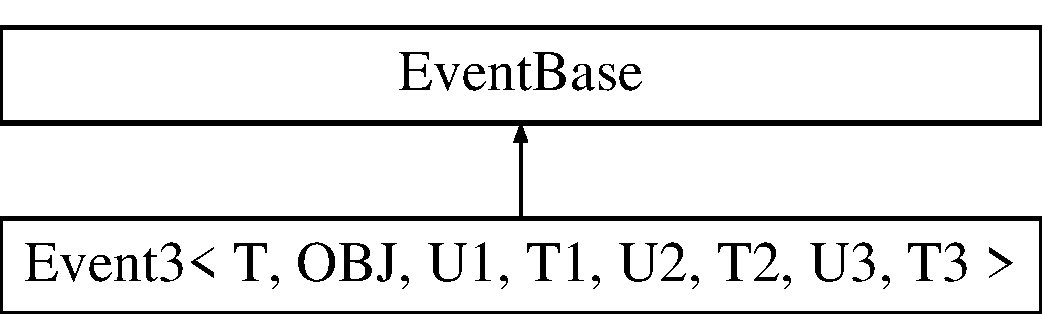
\includegraphics[height=2cm]{classEvent3}
\end{center}
\end{figure}
\subsection*{Public Member Functions}
\begin{CompactItemize}
\item 
\hyperlink{classEvent3_ab6870a823964c1843b897de6ce2057c}{Event3} (double t, void(T::$\ast$f)(U1, U2, U3), OBJ $\ast$obj0, T1 t1\_\-0, T2 t2\_\-0, T3 t3\_\-0)
\item 
void \hyperlink{classEvent3_1b9501d43723072952055c5abd9dc9be}{CallHandler} ()
\end{CompactItemize}
\subsection*{Public Attributes}
\begin{CompactItemize}
\item 
void(T::$\ast$ \hyperlink{classEvent3_2b4a3b7dbddc1dc7954942e7b2fe5745}{handler} )(U1, U2, U3)
\item 
OBJ $\ast$ \hyperlink{classEvent3_df320f52db00df12079299c183cb84d0}{obj}
\item 
T1 \hyperlink{classEvent3_d42449bd6cd4193bfb6557dc54c51eb8}{t1}
\item 
T2 \hyperlink{classEvent3_40afc3cdc9d75a5b3163795b78a42497}{t2}
\item 
T3 \hyperlink{classEvent3_7aa650837c6a02999bcad51817b144ef}{t3}
\end{CompactItemize}
\subsubsection*{template$<$typename T, typename OBJ, typename U1, typename T1, typename U2, typename T2, typename U3, typename T3$>$ class Event3$<$ T, OBJ, U1, T1, U2, T2, U3, T3 $>$}



\subsection{Constructor \& Destructor Documentation}
\hypertarget{classEvent3_ab6870a823964c1843b897de6ce2057c}{
\index{Event3@{Event3}!Event3@{Event3}}
\index{Event3@{Event3}!Event3@{Event3}}
\subsubsection[{Event3}]{\setlength{\rightskip}{0pt plus 5cm}template$<$typename T, typename OBJ, typename U1, typename T1, typename U2, typename T2, typename U3, typename T3$>$ {\bf Event3}$<$ T, OBJ, U1, T1, U2, T2, U3, T3 $>$::{\bf Event3} (double {\em t}, \/  void(T::$\ast$)(U1, U2, U3) {\em f}, \/  OBJ $\ast$ {\em obj0}, \/  T1 {\em t1\_\-0}, \/  T2 {\em t2\_\-0}, \/  T3 {\em t3\_\-0})\hspace{0.3cm}{\tt  \mbox{[}inline\mbox{]}}}}
\label{classEvent3_ab6870a823964c1843b897de6ce2057c}




\subsection{Member Function Documentation}
\hypertarget{classEvent3_1b9501d43723072952055c5abd9dc9be}{
\index{Event3@{Event3}!CallHandler@{CallHandler}}
\index{CallHandler@{CallHandler}!Event3@{Event3}}
\subsubsection[{CallHandler}]{\setlength{\rightskip}{0pt plus 5cm}template$<$typename T , typename OBJ , typename U1 , typename T1 , typename U2 , typename T2 , typename U3 , typename T3 $>$ void {\bf Event3}$<$ T, OBJ, U1, T1, U2, T2, U3, T3 $>$::CallHandler ()\hspace{0.3cm}{\tt  \mbox{[}inline, virtual\mbox{]}}}}
\label{classEvent3_1b9501d43723072952055c5abd9dc9be}




Implements \hyperlink{classEventBase_121ca64dec88c8d9589c064b0060d037}{EventBase}.

\subsection{Member Data Documentation}
\hypertarget{classEvent3_2b4a3b7dbddc1dc7954942e7b2fe5745}{
\index{Event3@{Event3}!handler@{handler}}
\index{handler@{handler}!Event3@{Event3}}
\subsubsection[{handler}]{\setlength{\rightskip}{0pt plus 5cm}template$<$typename T, typename OBJ, typename U1, typename T1, typename U2, typename T2, typename U3, typename T3$>$ void(T::$\ast$ {\bf Event3}$<$ T, OBJ, U1, T1, U2, T2, U3, T3 $>$::{\bf handler})(U1, U2, U3)}}
\label{classEvent3_2b4a3b7dbddc1dc7954942e7b2fe5745}


\hypertarget{classEvent3_df320f52db00df12079299c183cb84d0}{
\index{Event3@{Event3}!obj@{obj}}
\index{obj@{obj}!Event3@{Event3}}
\subsubsection[{obj}]{\setlength{\rightskip}{0pt plus 5cm}template$<$typename T, typename OBJ, typename U1, typename T1, typename U2, typename T2, typename U3, typename T3$>$ OBJ$\ast$ {\bf Event3}$<$ T, OBJ, U1, T1, U2, T2, U3, T3 $>$::{\bf obj}}}
\label{classEvent3_df320f52db00df12079299c183cb84d0}


\hypertarget{classEvent3_d42449bd6cd4193bfb6557dc54c51eb8}{
\index{Event3@{Event3}!t1@{t1}}
\index{t1@{t1}!Event3@{Event3}}
\subsubsection[{t1}]{\setlength{\rightskip}{0pt plus 5cm}template$<$typename T, typename OBJ, typename U1, typename T1, typename U2, typename T2, typename U3, typename T3$>$ T1 {\bf Event3}$<$ T, OBJ, U1, T1, U2, T2, U3, T3 $>$::{\bf t1}}}
\label{classEvent3_d42449bd6cd4193bfb6557dc54c51eb8}


\hypertarget{classEvent3_40afc3cdc9d75a5b3163795b78a42497}{
\index{Event3@{Event3}!t2@{t2}}
\index{t2@{t2}!Event3@{Event3}}
\subsubsection[{t2}]{\setlength{\rightskip}{0pt plus 5cm}template$<$typename T, typename OBJ, typename U1, typename T1, typename U2, typename T2, typename U3, typename T3$>$ T2 {\bf Event3}$<$ T, OBJ, U1, T1, U2, T2, U3, T3 $>$::{\bf t2}}}
\label{classEvent3_40afc3cdc9d75a5b3163795b78a42497}


\hypertarget{classEvent3_7aa650837c6a02999bcad51817b144ef}{
\index{Event3@{Event3}!t3@{t3}}
\index{t3@{t3}!Event3@{Event3}}
\subsubsection[{t3}]{\setlength{\rightskip}{0pt plus 5cm}template$<$typename T, typename OBJ, typename U1, typename T1, typename U2, typename T2, typename U3, typename T3$>$ T3 {\bf Event3}$<$ T, OBJ, U1, T1, U2, T2, U3, T3 $>$::{\bf t3}}}
\label{classEvent3_7aa650837c6a02999bcad51817b144ef}




The documentation for this class was generated from the following file:\begin{CompactItemize}
\item 
source/kernel/\hyperlink{simulator_8h}{simulator.h}\end{CompactItemize}

\hypertarget{classEvent3Stat}{
\section{Event3Stat$<$ U1, T1, U2, T2, U3, T3 $>$ Class Template Reference}
\label{classEvent3Stat}\index{Event3Stat@{Event3Stat}}
}
{\tt \#include $<$simulator.h$>$}

Inheritance diagram for Event3Stat$<$ U1, T1, U2, T2, U3, T3 $>$::\begin{figure}[H]
\begin{center}
\leavevmode
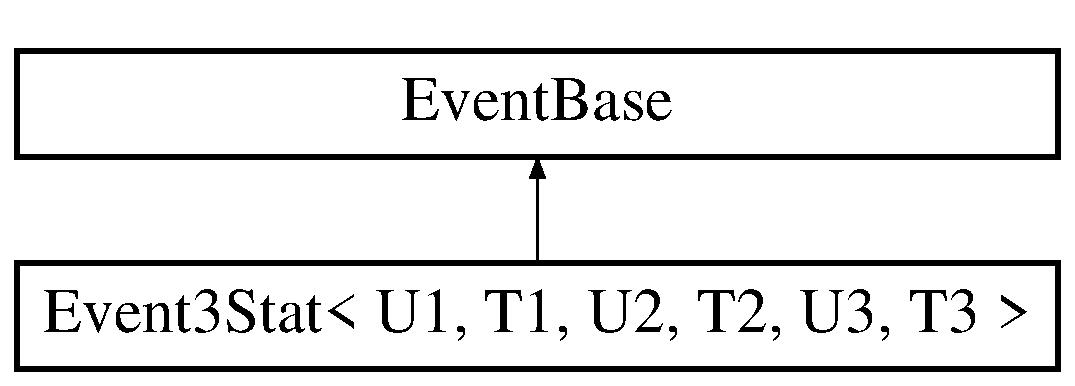
\includegraphics[height=2cm]{classEvent3Stat}
\end{center}
\end{figure}
\subsection*{Public Member Functions}
\begin{CompactItemize}
\item 
\hyperlink{classEvent3Stat_2bebf5183e80cc269d6282ea0569f8e0}{Event3Stat} (double t, void($\ast$f)(U1, U2, U3), T1 t1\_\-0, T2 t2\_\-0, T3 t3\_\-0)
\item 
void \hyperlink{classEvent3Stat_6901cb7acfdb3f021edd0a79c1766349}{CallHandler} ()
\end{CompactItemize}
\subsection*{Public Attributes}
\begin{CompactItemize}
\item 
void($\ast$ \hyperlink{classEvent3Stat_9a4bc9da2d5b2fac78aa4b01fc842218}{handler} )(U1, U2, U3)
\item 
T1 \hyperlink{classEvent3Stat_9fec91fe7e92c4eba9a09defa58d5431}{t1}
\item 
T2 \hyperlink{classEvent3Stat_33217dc4cdc50f79c062e8e42cd7f5d2}{t2}
\item 
T3 \hyperlink{classEvent3Stat_046cd41d71f5aa91fbf6e509602ebe13}{t3}
\end{CompactItemize}
\subsubsection*{template$<$typename U1, typename T1, typename U2, typename T2, typename U3, typename T3$>$ class Event3Stat$<$ U1, T1, U2, T2, U3, T3 $>$}



\subsection{Constructor \& Destructor Documentation}
\hypertarget{classEvent3Stat_2bebf5183e80cc269d6282ea0569f8e0}{
\index{Event3Stat@{Event3Stat}!Event3Stat@{Event3Stat}}
\index{Event3Stat@{Event3Stat}!Event3Stat@{Event3Stat}}
\subsubsection[{Event3Stat}]{\setlength{\rightskip}{0pt plus 5cm}template$<$typename U1, typename T1, typename U2, typename T2, typename U3, typename T3$>$ {\bf Event3Stat}$<$ U1, T1, U2, T2, U3, T3 $>$::{\bf Event3Stat} (double {\em t}, \/  void($\ast$)(U1, U2, U3) {\em f}, \/  T1 {\em t1\_\-0}, \/  T2 {\em t2\_\-0}, \/  T3 {\em t3\_\-0})\hspace{0.3cm}{\tt  \mbox{[}inline\mbox{]}}}}
\label{classEvent3Stat_2bebf5183e80cc269d6282ea0569f8e0}




\subsection{Member Function Documentation}
\hypertarget{classEvent3Stat_6901cb7acfdb3f021edd0a79c1766349}{
\index{Event3Stat@{Event3Stat}!CallHandler@{CallHandler}}
\index{CallHandler@{CallHandler}!Event3Stat@{Event3Stat}}
\subsubsection[{CallHandler}]{\setlength{\rightskip}{0pt plus 5cm}template$<$typename U1 , typename T1 , typename U2 , typename T2 , typename U3 , typename T3 $>$ void {\bf Event3Stat}$<$ U1, T1, U2, T2, U3, T3 $>$::CallHandler ()\hspace{0.3cm}{\tt  \mbox{[}inline, virtual\mbox{]}}}}
\label{classEvent3Stat_6901cb7acfdb3f021edd0a79c1766349}




Implements \hyperlink{classEventBase_121ca64dec88c8d9589c064b0060d037}{EventBase}.

\subsection{Member Data Documentation}
\hypertarget{classEvent3Stat_9a4bc9da2d5b2fac78aa4b01fc842218}{
\index{Event3Stat@{Event3Stat}!handler@{handler}}
\index{handler@{handler}!Event3Stat@{Event3Stat}}
\subsubsection[{handler}]{\setlength{\rightskip}{0pt plus 5cm}template$<$typename U1, typename T1, typename U2, typename T2, typename U3, typename T3$>$ void($\ast$ {\bf Event3Stat}$<$ U1, T1, U2, T2, U3, T3 $>$::{\bf handler})(U1, U2, U3)}}
\label{classEvent3Stat_9a4bc9da2d5b2fac78aa4b01fc842218}


\hypertarget{classEvent3Stat_9fec91fe7e92c4eba9a09defa58d5431}{
\index{Event3Stat@{Event3Stat}!t1@{t1}}
\index{t1@{t1}!Event3Stat@{Event3Stat}}
\subsubsection[{t1}]{\setlength{\rightskip}{0pt plus 5cm}template$<$typename U1, typename T1, typename U2, typename T2, typename U3, typename T3$>$ T1 {\bf Event3Stat}$<$ U1, T1, U2, T2, U3, T3 $>$::{\bf t1}}}
\label{classEvent3Stat_9fec91fe7e92c4eba9a09defa58d5431}


\hypertarget{classEvent3Stat_33217dc4cdc50f79c062e8e42cd7f5d2}{
\index{Event3Stat@{Event3Stat}!t2@{t2}}
\index{t2@{t2}!Event3Stat@{Event3Stat}}
\subsubsection[{t2}]{\setlength{\rightskip}{0pt plus 5cm}template$<$typename U1, typename T1, typename U2, typename T2, typename U3, typename T3$>$ T2 {\bf Event3Stat}$<$ U1, T1, U2, T2, U3, T3 $>$::{\bf t2}}}
\label{classEvent3Stat_33217dc4cdc50f79c062e8e42cd7f5d2}


\hypertarget{classEvent3Stat_046cd41d71f5aa91fbf6e509602ebe13}{
\index{Event3Stat@{Event3Stat}!t3@{t3}}
\index{t3@{t3}!Event3Stat@{Event3Stat}}
\subsubsection[{t3}]{\setlength{\rightskip}{0pt plus 5cm}template$<$typename U1, typename T1, typename U2, typename T2, typename U3, typename T3$>$ T3 {\bf Event3Stat}$<$ U1, T1, U2, T2, U3, T3 $>$::{\bf t3}}}
\label{classEvent3Stat_046cd41d71f5aa91fbf6e509602ebe13}




The documentation for this class was generated from the following file:\begin{CompactItemize}
\item 
source/kernel/\hyperlink{simulator_8h}{simulator.h}\end{CompactItemize}

\hypertarget{classEvent4}{
\section{Event4$<$ T, OBJ, U1, T1, U2, T2, U3, T3, U4, T4 $>$ Class Template Reference}
\label{classEvent4}\index{Event4@{Event4}}
}
{\tt \#include $<$simulator.h$>$}

Inheritance diagram for Event4$<$ T, OBJ, U1, T1, U2, T2, U3, T3, U4, T4 $>$::\begin{figure}[H]
\begin{center}
\leavevmode
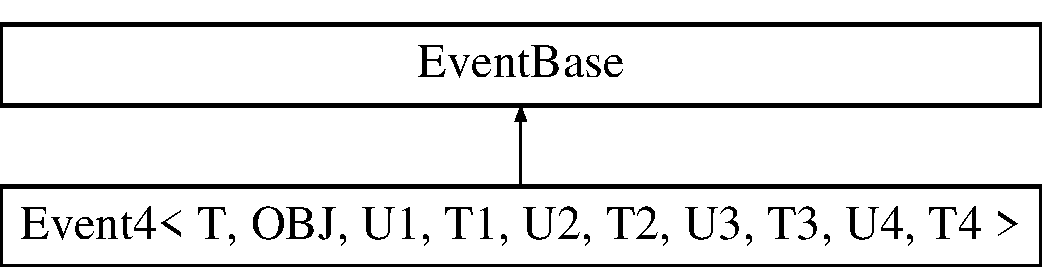
\includegraphics[height=2cm]{classEvent4}
\end{center}
\end{figure}
\subsection*{Public Member Functions}
\begin{CompactItemize}
\item 
\hyperlink{classEvent4_44d546a1df3e3421086701d66b103e3c}{Event4} (double t, void(T::$\ast$f)(U1, U2, U3, U4), OBJ $\ast$obj0, T1 t1\_\-0, T2 t2\_\-0, T3 t3\_\-0, T4 t4\_\-0)
\item 
void \hyperlink{classEvent4_69f98edf52e4f93f5cf0e0d5464f6ce0}{CallHandler} ()
\end{CompactItemize}
\subsection*{Public Attributes}
\begin{CompactItemize}
\item 
void(T::$\ast$ \hyperlink{classEvent4_13bc21430e9b5e4f41d9df447f455a57}{handler} )(U1, U2, U3, U4)
\item 
OBJ $\ast$ \hyperlink{classEvent4_214fd485cf467a8b3e7f48de2cce982a}{obj}
\item 
T1 \hyperlink{classEvent4_71f46004ef408ffe9c15d8eb4c295e9e}{t1}
\item 
T2 \hyperlink{classEvent4_61865aa3d8420f7e3cefab5dcb750f03}{t2}
\item 
T3 \hyperlink{classEvent4_44d2b08b43f20fac8f5cb3666e63cc52}{t3}
\item 
T4 \hyperlink{classEvent4_0a7fbdc85c74aececd3b997574ac0875}{t4}
\end{CompactItemize}
\subsubsection*{template$<$typename T, typename OBJ, typename U1, typename T1, typename U2, typename T2, typename U3, typename T3, typename U4, typename T4$>$ class Event4$<$ T, OBJ, U1, T1, U2, T2, U3, T3, U4, T4 $>$}



\subsection{Constructor \& Destructor Documentation}
\hypertarget{classEvent4_44d546a1df3e3421086701d66b103e3c}{
\index{Event4@{Event4}!Event4@{Event4}}
\index{Event4@{Event4}!Event4@{Event4}}
\subsubsection[{Event4}]{\setlength{\rightskip}{0pt plus 5cm}template$<$typename T, typename OBJ, typename U1, typename T1, typename U2, typename T2, typename U3, typename T3, typename U4, typename T4$>$ {\bf Event4}$<$ T, OBJ, U1, T1, U2, T2, U3, T3, U4, T4 $>$::{\bf Event4} (double {\em t}, \/  void(T::$\ast$)(U1, U2, U3, U4) {\em f}, \/  OBJ $\ast$ {\em obj0}, \/  T1 {\em t1\_\-0}, \/  T2 {\em t2\_\-0}, \/  T3 {\em t3\_\-0}, \/  T4 {\em t4\_\-0})\hspace{0.3cm}{\tt  \mbox{[}inline\mbox{]}}}}
\label{classEvent4_44d546a1df3e3421086701d66b103e3c}




\subsection{Member Function Documentation}
\hypertarget{classEvent4_69f98edf52e4f93f5cf0e0d5464f6ce0}{
\index{Event4@{Event4}!CallHandler@{CallHandler}}
\index{CallHandler@{CallHandler}!Event4@{Event4}}
\subsubsection[{CallHandler}]{\setlength{\rightskip}{0pt plus 5cm}template$<$typename T , typename OBJ , typename U1 , typename T1 , typename U2 , typename T2 , typename U3 , typename T3 , typename U4 , typename T4 $>$ void {\bf Event4}$<$ T, OBJ, U1, T1, U2, T2, U3, T3, U4, T4 $>$::CallHandler ()\hspace{0.3cm}{\tt  \mbox{[}inline, virtual\mbox{]}}}}
\label{classEvent4_69f98edf52e4f93f5cf0e0d5464f6ce0}




Implements \hyperlink{classEventBase_121ca64dec88c8d9589c064b0060d037}{EventBase}.

\subsection{Member Data Documentation}
\hypertarget{classEvent4_13bc21430e9b5e4f41d9df447f455a57}{
\index{Event4@{Event4}!handler@{handler}}
\index{handler@{handler}!Event4@{Event4}}
\subsubsection[{handler}]{\setlength{\rightskip}{0pt plus 5cm}template$<$typename T, typename OBJ, typename U1, typename T1, typename U2, typename T2, typename U3, typename T3, typename U4, typename T4$>$ void(T::$\ast$ {\bf Event4}$<$ T, OBJ, U1, T1, U2, T2, U3, T3, U4, T4 $>$::{\bf handler})(U1, U2, U3, U4)}}
\label{classEvent4_13bc21430e9b5e4f41d9df447f455a57}


\hypertarget{classEvent4_214fd485cf467a8b3e7f48de2cce982a}{
\index{Event4@{Event4}!obj@{obj}}
\index{obj@{obj}!Event4@{Event4}}
\subsubsection[{obj}]{\setlength{\rightskip}{0pt plus 5cm}template$<$typename T, typename OBJ, typename U1, typename T1, typename U2, typename T2, typename U3, typename T3, typename U4, typename T4$>$ OBJ$\ast$ {\bf Event4}$<$ T, OBJ, U1, T1, U2, T2, U3, T3, U4, T4 $>$::{\bf obj}}}
\label{classEvent4_214fd485cf467a8b3e7f48de2cce982a}


\hypertarget{classEvent4_71f46004ef408ffe9c15d8eb4c295e9e}{
\index{Event4@{Event4}!t1@{t1}}
\index{t1@{t1}!Event4@{Event4}}
\subsubsection[{t1}]{\setlength{\rightskip}{0pt plus 5cm}template$<$typename T, typename OBJ, typename U1, typename T1, typename U2, typename T2, typename U3, typename T3, typename U4, typename T4$>$ T1 {\bf Event4}$<$ T, OBJ, U1, T1, U2, T2, U3, T3, U4, T4 $>$::{\bf t1}}}
\label{classEvent4_71f46004ef408ffe9c15d8eb4c295e9e}


\hypertarget{classEvent4_61865aa3d8420f7e3cefab5dcb750f03}{
\index{Event4@{Event4}!t2@{t2}}
\index{t2@{t2}!Event4@{Event4}}
\subsubsection[{t2}]{\setlength{\rightskip}{0pt plus 5cm}template$<$typename T, typename OBJ, typename U1, typename T1, typename U2, typename T2, typename U3, typename T3, typename U4, typename T4$>$ T2 {\bf Event4}$<$ T, OBJ, U1, T1, U2, T2, U3, T3, U4, T4 $>$::{\bf t2}}}
\label{classEvent4_61865aa3d8420f7e3cefab5dcb750f03}


\hypertarget{classEvent4_44d2b08b43f20fac8f5cb3666e63cc52}{
\index{Event4@{Event4}!t3@{t3}}
\index{t3@{t3}!Event4@{Event4}}
\subsubsection[{t3}]{\setlength{\rightskip}{0pt plus 5cm}template$<$typename T, typename OBJ, typename U1, typename T1, typename U2, typename T2, typename U3, typename T3, typename U4, typename T4$>$ T3 {\bf Event4}$<$ T, OBJ, U1, T1, U2, T2, U3, T3, U4, T4 $>$::{\bf t3}}}
\label{classEvent4_44d2b08b43f20fac8f5cb3666e63cc52}


\hypertarget{classEvent4_0a7fbdc85c74aececd3b997574ac0875}{
\index{Event4@{Event4}!t4@{t4}}
\index{t4@{t4}!Event4@{Event4}}
\subsubsection[{t4}]{\setlength{\rightskip}{0pt plus 5cm}template$<$typename T, typename OBJ, typename U1, typename T1, typename U2, typename T2, typename U3, typename T3, typename U4, typename T4$>$ T4 {\bf Event4}$<$ T, OBJ, U1, T1, U2, T2, U3, T3, U4, T4 $>$::{\bf t4}}}
\label{classEvent4_0a7fbdc85c74aececd3b997574ac0875}




The documentation for this class was generated from the following file:\begin{CompactItemize}
\item 
source/kernel/\hyperlink{simulator_8h}{simulator.h}\end{CompactItemize}

\hypertarget{classEvent4Stat}{
\section{Event4Stat$<$ U1, T1, U2, T2, U3, T3, U4, T4 $>$ Class Template Reference}
\label{classEvent4Stat}\index{Event4Stat@{Event4Stat}}
}
{\tt \#include $<$simulator.h$>$}

Inheritance diagram for Event4Stat$<$ U1, T1, U2, T2, U3, T3, U4, T4 $>$::\begin{figure}[H]
\begin{center}
\leavevmode
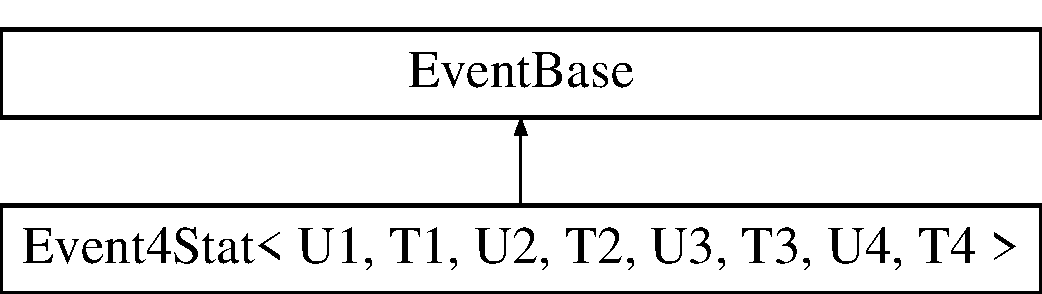
\includegraphics[height=2cm]{classEvent4Stat}
\end{center}
\end{figure}
\subsection*{Public Member Functions}
\begin{CompactItemize}
\item 
\hyperlink{classEvent4Stat_ef35a029c53b7da66278dd753d15a6d3}{Event4Stat} (double t, void($\ast$f)(U1, U2, U3, U4), T1 t1\_\-0, T2 t2\_\-0, T3 t3\_\-0, T4 t4\_\-0)
\item 
void \hyperlink{classEvent4Stat_4dfca297cb5eede83851898b5c4f2f76}{CallHandler} ()
\end{CompactItemize}
\subsection*{Public Attributes}
\begin{CompactItemize}
\item 
void($\ast$ \hyperlink{classEvent4Stat_77188f75f46284cde2b6baa8851e9487}{handler} )(U1, U2, U3, U4)
\item 
T1 \hyperlink{classEvent4Stat_82b1a4255a770e482d4aa975713b5150}{t1}
\item 
T2 \hyperlink{classEvent4Stat_aaa8d8169956ad7f816594902579fa52}{t2}
\item 
T3 \hyperlink{classEvent4Stat_0cb1a5a34eac05d95539aaae5dba162d}{t3}
\item 
T4 \hyperlink{classEvent4Stat_4812a9e029fb2e460a2bebdf253d7c7d}{t4}
\end{CompactItemize}
\subsubsection*{template$<$typename U1, typename T1, typename U2, typename T2, typename U3, typename T3, typename U4, typename T4$>$ class Event4Stat$<$ U1, T1, U2, T2, U3, T3, U4, T4 $>$}



\subsection{Constructor \& Destructor Documentation}
\hypertarget{classEvent4Stat_ef35a029c53b7da66278dd753d15a6d3}{
\index{Event4Stat@{Event4Stat}!Event4Stat@{Event4Stat}}
\index{Event4Stat@{Event4Stat}!Event4Stat@{Event4Stat}}
\subsubsection[{Event4Stat}]{\setlength{\rightskip}{0pt plus 5cm}template$<$typename U1, typename T1, typename U2, typename T2, typename U3, typename T3, typename U4, typename T4$>$ {\bf Event4Stat}$<$ U1, T1, U2, T2, U3, T3, U4, T4 $>$::{\bf Event4Stat} (double {\em t}, \/  void($\ast$)(U1, U2, U3, U4) {\em f}, \/  T1 {\em t1\_\-0}, \/  T2 {\em t2\_\-0}, \/  T3 {\em t3\_\-0}, \/  T4 {\em t4\_\-0})\hspace{0.3cm}{\tt  \mbox{[}inline\mbox{]}}}}
\label{classEvent4Stat_ef35a029c53b7da66278dd753d15a6d3}




\subsection{Member Function Documentation}
\hypertarget{classEvent4Stat_4dfca297cb5eede83851898b5c4f2f76}{
\index{Event4Stat@{Event4Stat}!CallHandler@{CallHandler}}
\index{CallHandler@{CallHandler}!Event4Stat@{Event4Stat}}
\subsubsection[{CallHandler}]{\setlength{\rightskip}{0pt plus 5cm}template$<$typename U1 , typename T1 , typename U2 , typename T2 , typename U3 , typename T3 , typename U4 , typename T4 $>$ void {\bf Event4Stat}$<$ U1, T1, U2, T2, U3, T3, U4, T4 $>$::CallHandler ()\hspace{0.3cm}{\tt  \mbox{[}inline, virtual\mbox{]}}}}
\label{classEvent4Stat_4dfca297cb5eede83851898b5c4f2f76}




Implements \hyperlink{classEventBase_121ca64dec88c8d9589c064b0060d037}{EventBase}.

\subsection{Member Data Documentation}
\hypertarget{classEvent4Stat_77188f75f46284cde2b6baa8851e9487}{
\index{Event4Stat@{Event4Stat}!handler@{handler}}
\index{handler@{handler}!Event4Stat@{Event4Stat}}
\subsubsection[{handler}]{\setlength{\rightskip}{0pt plus 5cm}template$<$typename U1, typename T1, typename U2, typename T2, typename U3, typename T3, typename U4, typename T4$>$ void($\ast$ {\bf Event4Stat}$<$ U1, T1, U2, T2, U3, T3, U4, T4 $>$::{\bf handler})(U1, U2, U3, U4)}}
\label{classEvent4Stat_77188f75f46284cde2b6baa8851e9487}


\hypertarget{classEvent4Stat_82b1a4255a770e482d4aa975713b5150}{
\index{Event4Stat@{Event4Stat}!t1@{t1}}
\index{t1@{t1}!Event4Stat@{Event4Stat}}
\subsubsection[{t1}]{\setlength{\rightskip}{0pt plus 5cm}template$<$typename U1, typename T1, typename U2, typename T2, typename U3, typename T3, typename U4, typename T4$>$ T1 {\bf Event4Stat}$<$ U1, T1, U2, T2, U3, T3, U4, T4 $>$::{\bf t1}}}
\label{classEvent4Stat_82b1a4255a770e482d4aa975713b5150}


\hypertarget{classEvent4Stat_aaa8d8169956ad7f816594902579fa52}{
\index{Event4Stat@{Event4Stat}!t2@{t2}}
\index{t2@{t2}!Event4Stat@{Event4Stat}}
\subsubsection[{t2}]{\setlength{\rightskip}{0pt plus 5cm}template$<$typename U1, typename T1, typename U2, typename T2, typename U3, typename T3, typename U4, typename T4$>$ T2 {\bf Event4Stat}$<$ U1, T1, U2, T2, U3, T3, U4, T4 $>$::{\bf t2}}}
\label{classEvent4Stat_aaa8d8169956ad7f816594902579fa52}


\hypertarget{classEvent4Stat_0cb1a5a34eac05d95539aaae5dba162d}{
\index{Event4Stat@{Event4Stat}!t3@{t3}}
\index{t3@{t3}!Event4Stat@{Event4Stat}}
\subsubsection[{t3}]{\setlength{\rightskip}{0pt plus 5cm}template$<$typename U1, typename T1, typename U2, typename T2, typename U3, typename T3, typename U4, typename T4$>$ T3 {\bf Event4Stat}$<$ U1, T1, U2, T2, U3, T3, U4, T4 $>$::{\bf t3}}}
\label{classEvent4Stat_0cb1a5a34eac05d95539aaae5dba162d}


\hypertarget{classEvent4Stat_4812a9e029fb2e460a2bebdf253d7c7d}{
\index{Event4Stat@{Event4Stat}!t4@{t4}}
\index{t4@{t4}!Event4Stat@{Event4Stat}}
\subsubsection[{t4}]{\setlength{\rightskip}{0pt plus 5cm}template$<$typename U1, typename T1, typename U2, typename T2, typename U3, typename T3, typename U4, typename T4$>$ T4 {\bf Event4Stat}$<$ U1, T1, U2, T2, U3, T3, U4, T4 $>$::{\bf t4}}}
\label{classEvent4Stat_4812a9e029fb2e460a2bebdf253d7c7d}




The documentation for this class was generated from the following file:\begin{CompactItemize}
\item 
source/kernel/\hyperlink{simulator_8h}{simulator.h}\end{CompactItemize}

\hypertarget{classevent__less}{
\section{event\_\-less Class Reference}
\label{classevent__less}\index{event\_\-less@{event\_\-less}}
}
{\tt \#include $<$simulator.h$>$}

\subsection*{Public Member Functions}
\begin{CompactItemize}
\item 
\hyperlink{classevent__less_b721525a6ed5ec4551920178ea91726c}{event\_\-less} ()
\item 
bool \hyperlink{classevent__less_280b704ba9909d43362de372d0a45523}{operator()} (\hyperlink{classEventBase}{EventBase} $\ast$const \&l, const \hyperlink{classEventBase}{EventBase} $\ast$const \&r) const 
\end{CompactItemize}


\subsection{Constructor \& Destructor Documentation}
\hypertarget{classevent__less_b721525a6ed5ec4551920178ea91726c}{
\index{event\_\-less@{event\_\-less}!event\_\-less@{event\_\-less}}
\index{event\_\-less@{event\_\-less}!event_less@{event\_\-less}}
\subsubsection[{event\_\-less}]{\setlength{\rightskip}{0pt plus 5cm}event\_\-less::event\_\-less ()\hspace{0.3cm}{\tt  \mbox{[}inline\mbox{]}}}}
\label{classevent__less_b721525a6ed5ec4551920178ea91726c}




\subsection{Member Function Documentation}
\hypertarget{classevent__less_280b704ba9909d43362de372d0a45523}{
\index{event\_\-less@{event\_\-less}!operator()@{operator()}}
\index{operator()@{operator()}!event_less@{event\_\-less}}
\subsubsection[{operator()}]{\setlength{\rightskip}{0pt plus 5cm}bool event\_\-less::operator() ({\bf EventBase} $\ast$const \& {\em l}, \/  const {\bf EventBase} $\ast$const \& {\em r}) const\hspace{0.3cm}{\tt  \mbox{[}inline\mbox{]}}}}
\label{classevent__less_280b704ba9909d43362de372d0a45523}




The documentation for this class was generated from the following file:\begin{CompactItemize}
\item 
source/kernel/\hyperlink{simulator_8h}{simulator.h}\end{CompactItemize}

\hypertarget{classEventBase}{
\section{EventBase Class Reference}
\label{classEventBase}\index{EventBase@{EventBase}}
}
{\tt \#include $<$simulator.h$>$}

Inheritance diagram for EventBase::\begin{figure}[H]
\begin{center}
\leavevmode
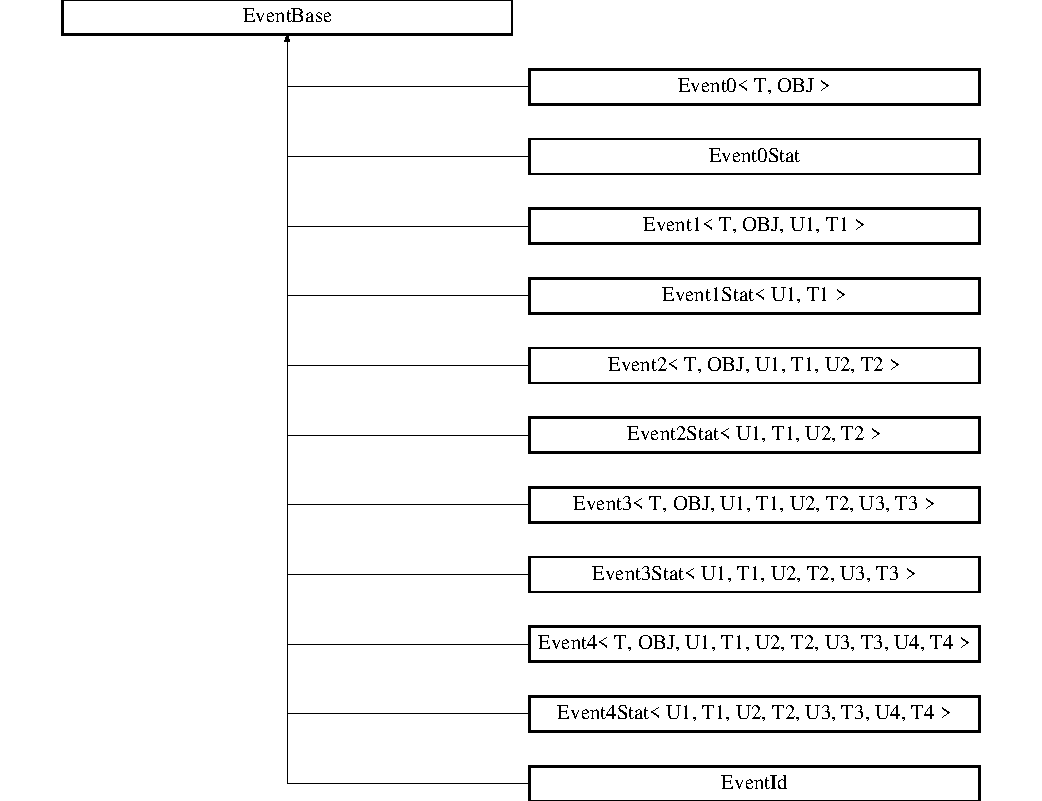
\includegraphics[height=10.7692cm]{classEventBase}
\end{center}
\end{figure}
\subsection*{Public Member Functions}
\begin{CompactItemize}
\item 
\hyperlink{classEventBase_e95c43af6512ec2ab717eeb240ecad0a}{EventBase} (double t)
\item 
\hyperlink{classEventBase_0213a35ffa61ce4f7066128e89da5af8}{EventBase} (double t, int u)
\item 
virtual void \hyperlink{classEventBase_121ca64dec88c8d9589c064b0060d037}{CallHandler} ()=0
\end{CompactItemize}
\subsection*{Public Attributes}
\begin{CompactItemize}
\item 
double \hyperlink{classEventBase_b64e6661c521961aa3a18b8ac34566ed}{time}
\item 
int \hyperlink{classEventBase_f22f14be6b15b6f99d347b8726a7613a}{uid}
\end{CompactItemize}
\subsection*{Static Public Attributes}
\begin{CompactItemize}
\item 
static int \hyperlink{classEventBase_22a8c15e90a68f16042fd7b12dfe5935}{nextUID} = 0
\end{CompactItemize}


\subsection{Constructor \& Destructor Documentation}
\hypertarget{classEventBase_e95c43af6512ec2ab717eeb240ecad0a}{
\index{EventBase@{EventBase}!EventBase@{EventBase}}
\index{EventBase@{EventBase}!EventBase@{EventBase}}
\subsubsection[{EventBase}]{\setlength{\rightskip}{0pt plus 5cm}EventBase::EventBase (double {\em t})\hspace{0.3cm}{\tt  \mbox{[}inline\mbox{]}}}}
\label{classEventBase_e95c43af6512ec2ab717eeb240ecad0a}


\hypertarget{classEventBase_0213a35ffa61ce4f7066128e89da5af8}{
\index{EventBase@{EventBase}!EventBase@{EventBase}}
\index{EventBase@{EventBase}!EventBase@{EventBase}}
\subsubsection[{EventBase}]{\setlength{\rightskip}{0pt plus 5cm}EventBase::EventBase (double {\em t}, \/  int {\em u})\hspace{0.3cm}{\tt  \mbox{[}inline\mbox{]}}}}
\label{classEventBase_0213a35ffa61ce4f7066128e89da5af8}




\subsection{Member Function Documentation}
\hypertarget{classEventBase_121ca64dec88c8d9589c064b0060d037}{
\index{EventBase@{EventBase}!CallHandler@{CallHandler}}
\index{CallHandler@{CallHandler}!EventBase@{EventBase}}
\subsubsection[{CallHandler}]{\setlength{\rightskip}{0pt plus 5cm}virtual void EventBase::CallHandler ()\hspace{0.3cm}{\tt  \mbox{[}pure virtual\mbox{]}}}}
\label{classEventBase_121ca64dec88c8d9589c064b0060d037}




Implemented in \hyperlink{classEventId_8627fa7b92746ddd1bd8b582b68fb3d1}{EventId}, \hyperlink{classEvent0_77176d1040ed4cc48fa750c4854212b9}{Event0$<$ T, OBJ $>$}, \hyperlink{classEvent1_6d7e716e16ab6ee6672807250860cdd8}{Event1$<$ T, OBJ, U1, T1 $>$}, \hyperlink{classEvent2_428b314837eee680fa435cad61944af3}{Event2$<$ T, OBJ, U1, T1, U2, T2 $>$}, \hyperlink{classEvent3_1b9501d43723072952055c5abd9dc9be}{Event3$<$ T, OBJ, U1, T1, U2, T2, U3, T3 $>$}, \hyperlink{classEvent4_69f98edf52e4f93f5cf0e0d5464f6ce0}{Event4$<$ T, OBJ, U1, T1, U2, T2, U3, T3, U4, T4 $>$}, \hyperlink{classEvent0Stat_0cf3e0d44a1c04ee73a8a93a50ca05a1}{Event0Stat}, \hyperlink{classEvent1Stat_d39942fb840e55ee829decdf1927eadf}{Event1Stat$<$ U1, T1 $>$}, \hyperlink{classEvent2Stat_84e6e9e412678507da3b2bde8e6a157a}{Event2Stat$<$ U1, T1, U2, T2 $>$}, \hyperlink{classEvent3Stat_6901cb7acfdb3f021edd0a79c1766349}{Event3Stat$<$ U1, T1, U2, T2, U3, T3 $>$}, and \hyperlink{classEvent4Stat_4dfca297cb5eede83851898b5c4f2f76}{Event4Stat$<$ U1, T1, U2, T2, U3, T3, U4, T4 $>$}.

\subsection{Member Data Documentation}
\hypertarget{classEventBase_22a8c15e90a68f16042fd7b12dfe5935}{
\index{EventBase@{EventBase}!nextUID@{nextUID}}
\index{nextUID@{nextUID}!EventBase@{EventBase}}
\subsubsection[{nextUID}]{\setlength{\rightskip}{0pt plus 5cm}int {\bf EventBase::nextUID} = 0\hspace{0.3cm}{\tt  \mbox{[}static\mbox{]}}}}
\label{classEventBase_22a8c15e90a68f16042fd7b12dfe5935}


\hypertarget{classEventBase_b64e6661c521961aa3a18b8ac34566ed}{
\index{EventBase@{EventBase}!time@{time}}
\index{time@{time}!EventBase@{EventBase}}
\subsubsection[{time}]{\setlength{\rightskip}{0pt plus 5cm}double {\bf EventBase::time}}}
\label{classEventBase_b64e6661c521961aa3a18b8ac34566ed}


\hypertarget{classEventBase_f22f14be6b15b6f99d347b8726a7613a}{
\index{EventBase@{EventBase}!uid@{uid}}
\index{uid@{uid}!EventBase@{EventBase}}
\subsubsection[{uid}]{\setlength{\rightskip}{0pt plus 5cm}int {\bf EventBase::uid}}}
\label{classEventBase_f22f14be6b15b6f99d347b8726a7613a}




The documentation for this class was generated from the following files:\begin{CompactItemize}
\item 
source/kernel/\hyperlink{simulator_8h}{simulator.h}\item 
source/kernel/\hyperlink{simulator_8cc}{simulator.cc}\end{CompactItemize}

\hypertarget{classEventId}{
\section{EventId Class Reference}
\label{classEventId}\index{EventId@{EventId}}
}
{\tt \#include $<$simulator.h$>$}

Inheritance diagram for EventId::\begin{figure}[H]
\begin{center}
\leavevmode
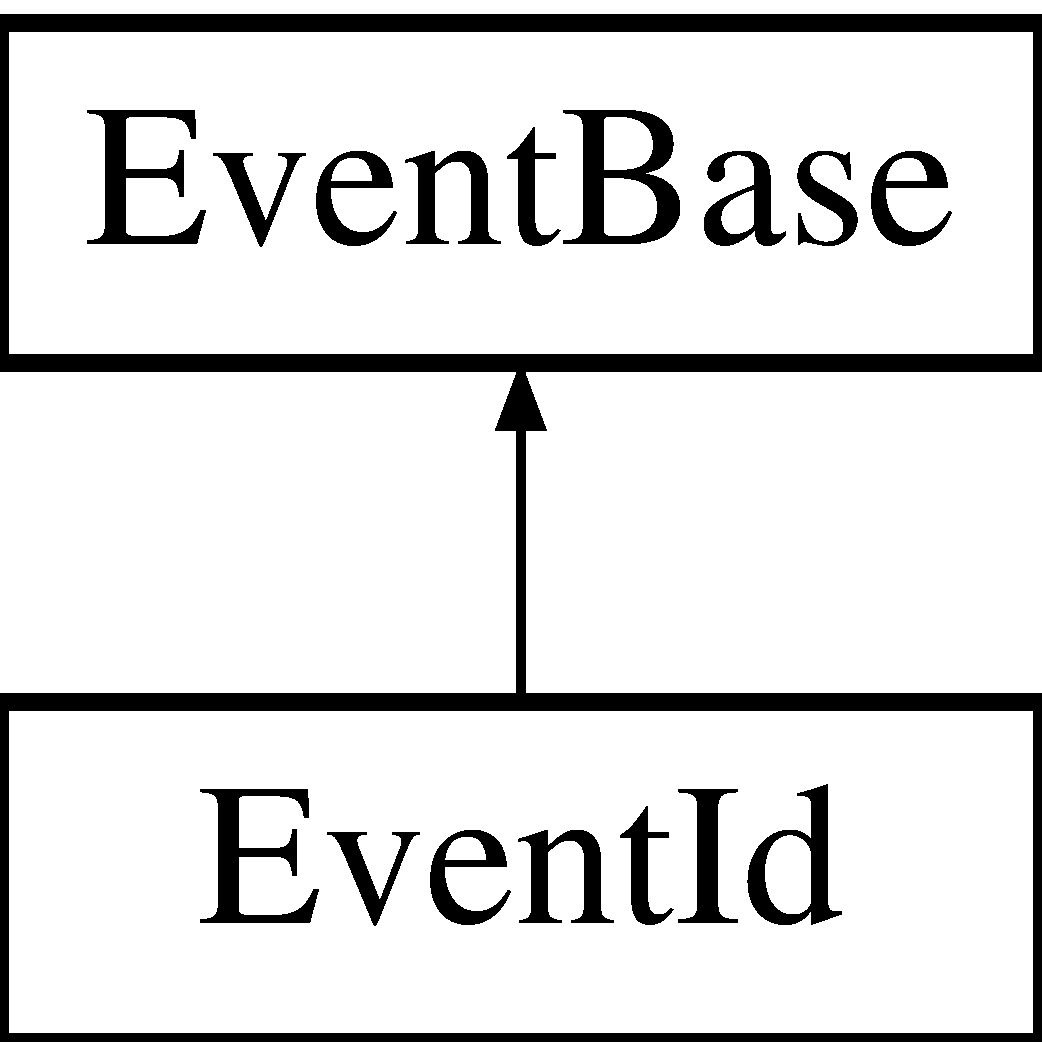
\includegraphics[height=2cm]{classEventId}
\end{center}
\end{figure}
\subsection*{Public Member Functions}
\begin{CompactItemize}
\item 
\hyperlink{classEventId_e9003f33346c511981dee0dd7e6ad459}{EventId} (double t, int u)
\item 
void \hyperlink{classEventId_8627fa7b92746ddd1bd8b582b68fb3d1}{CallHandler} ()
\end{CompactItemize}


\subsection{Constructor \& Destructor Documentation}
\hypertarget{classEventId_e9003f33346c511981dee0dd7e6ad459}{
\index{EventId@{EventId}!EventId@{EventId}}
\index{EventId@{EventId}!EventId@{EventId}}
\subsubsection[{EventId}]{\setlength{\rightskip}{0pt plus 5cm}EventId::EventId (double {\em t}, \/  int {\em u})\hspace{0.3cm}{\tt  \mbox{[}inline\mbox{]}}}}
\label{classEventId_e9003f33346c511981dee0dd7e6ad459}




\subsection{Member Function Documentation}
\hypertarget{classEventId_8627fa7b92746ddd1bd8b582b68fb3d1}{
\index{EventId@{EventId}!CallHandler@{CallHandler}}
\index{CallHandler@{CallHandler}!EventId@{EventId}}
\subsubsection[{CallHandler}]{\setlength{\rightskip}{0pt plus 5cm}void EventId::CallHandler ()\hspace{0.3cm}{\tt  \mbox{[}inline, virtual\mbox{]}}}}
\label{classEventId_8627fa7b92746ddd1bd8b582b68fb3d1}




Implements \hyperlink{classEventBase_121ca64dec88c8d9589c064b0060d037}{EventBase}.

The documentation for this class was generated from the following file:\begin{CompactItemize}
\item 
source/kernel/\hyperlink{simulator_8h}{simulator.h}\end{CompactItemize}

\hypertarget{classExponential}{
\section{Exponential Class Reference}
\label{classExponential}\index{Exponential@{Exponential}}
}
{\tt \#include $<$rng.hpp$>$}

Inheritance diagram for Exponential::\begin{figure}[H]
\begin{center}
\leavevmode
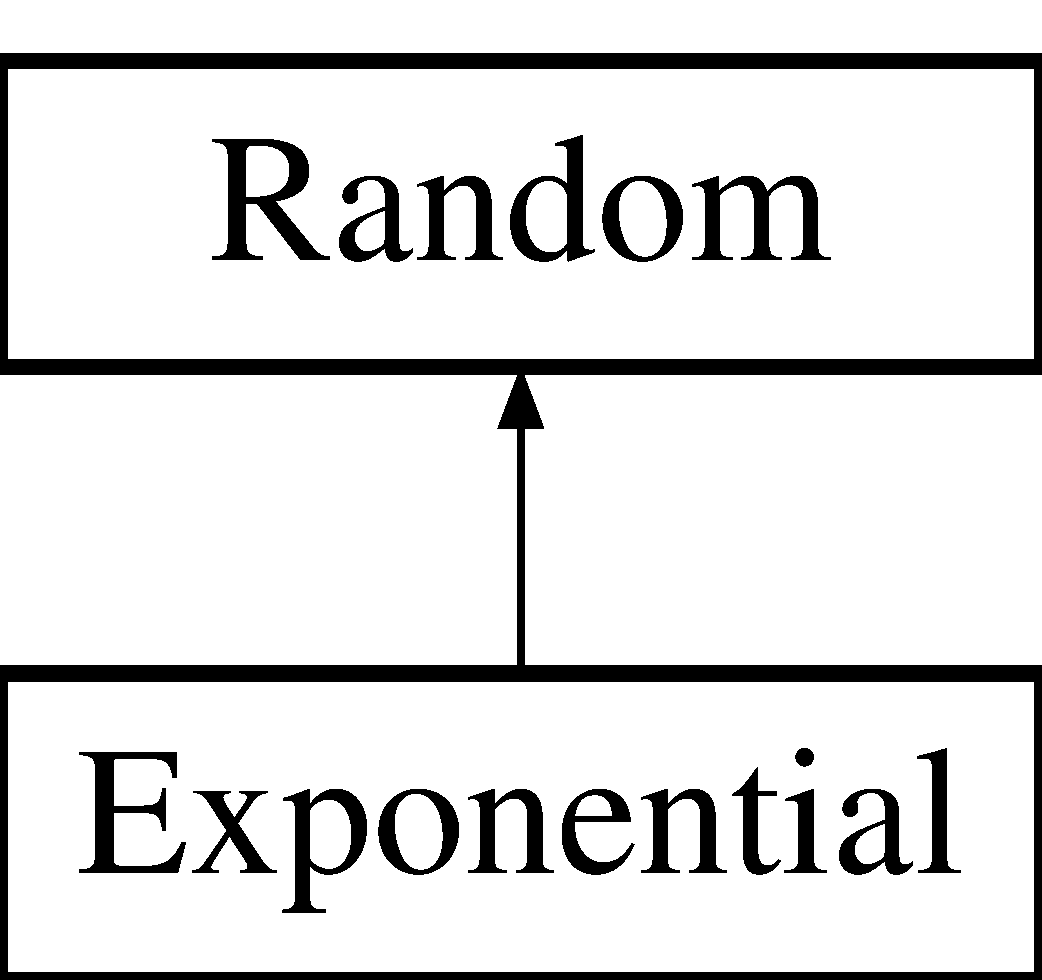
\includegraphics[height=2cm]{classExponential}
\end{center}
\end{figure}
\subsection*{Public Member Functions}
\begin{CompactItemize}
\item 
\hyperlink{classExponential_bc75eaef5b5f89656c4aa406aceb3c27}{Exponential} ()
\item 
\hyperlink{classExponential_62d588bfc48c87b4cf30badcd306cfa3}{Exponential} (\hyperlink{rng_8hpp_ad41e7f5d86b1109b6a6a032c86cdd3f}{Random\_\-t} m)
\item 
\hyperlink{classExponential_469f22991fc0e7192e395ffde9b6a1ce}{Exponential} (\hyperlink{rng_8hpp_ad41e7f5d86b1109b6a6a032c86cdd3f}{Random\_\-t} m, \hyperlink{rng_8hpp_ad41e7f5d86b1109b6a6a032c86cdd3f}{Random\_\-t} b)
\item 
\hyperlink{classExponential_5b49e6e7f936a44f88a54aa3ff5e6e61}{Exponential} (const \hyperlink{classExponential}{Exponential} \&c)
\item 
virtual \hyperlink{rng_8hpp_ad41e7f5d86b1109b6a6a032c86cdd3f}{Random\_\-t} \hyperlink{classExponential_c2ad56e3dc3e65673cb54cab95d34a53}{Value} ()
\item 
virtual \hyperlink{classRandom}{Random} $\ast$ \hyperlink{classExponential_f7c51eb8cb4fee14f659a55f994e981f}{Copy} () const 
\end{CompactItemize}


\subsection{Constructor \& Destructor Documentation}
\hypertarget{classExponential_bc75eaef5b5f89656c4aa406aceb3c27}{
\index{Exponential@{Exponential}!Exponential@{Exponential}}
\index{Exponential@{Exponential}!Exponential@{Exponential}}
\subsubsection[{Exponential}]{\setlength{\rightskip}{0pt plus 5cm}Exponential::Exponential ()\hspace{0.3cm}{\tt  \mbox{[}inline\mbox{]}}}}
\label{classExponential_bc75eaef5b5f89656c4aa406aceb3c27}


\hypertarget{classExponential_62d588bfc48c87b4cf30badcd306cfa3}{
\index{Exponential@{Exponential}!Exponential@{Exponential}}
\index{Exponential@{Exponential}!Exponential@{Exponential}}
\subsubsection[{Exponential}]{\setlength{\rightskip}{0pt plus 5cm}Exponential::Exponential ({\bf Random\_\-t} {\em m})\hspace{0.3cm}{\tt  \mbox{[}inline, explicit\mbox{]}}}}
\label{classExponential_62d588bfc48c87b4cf30badcd306cfa3}


\hypertarget{classExponential_469f22991fc0e7192e395ffde9b6a1ce}{
\index{Exponential@{Exponential}!Exponential@{Exponential}}
\index{Exponential@{Exponential}!Exponential@{Exponential}}
\subsubsection[{Exponential}]{\setlength{\rightskip}{0pt plus 5cm}Exponential::Exponential ({\bf Random\_\-t} {\em m}, \/  {\bf Random\_\-t} {\em b})\hspace{0.3cm}{\tt  \mbox{[}inline\mbox{]}}}}
\label{classExponential_469f22991fc0e7192e395ffde9b6a1ce}


\hypertarget{classExponential_5b49e6e7f936a44f88a54aa3ff5e6e61}{
\index{Exponential@{Exponential}!Exponential@{Exponential}}
\index{Exponential@{Exponential}!Exponential@{Exponential}}
\subsubsection[{Exponential}]{\setlength{\rightskip}{0pt plus 5cm}Exponential::Exponential (const {\bf Exponential} \& {\em c})\hspace{0.3cm}{\tt  \mbox{[}inline\mbox{]}}}}
\label{classExponential_5b49e6e7f936a44f88a54aa3ff5e6e61}




\subsection{Member Function Documentation}
\hypertarget{classExponential_f7c51eb8cb4fee14f659a55f994e981f}{
\index{Exponential@{Exponential}!Copy@{Copy}}
\index{Copy@{Copy}!Exponential@{Exponential}}
\subsubsection[{Copy}]{\setlength{\rightskip}{0pt plus 5cm}{\bf Random} $\ast$ Exponential::Copy () const\hspace{0.3cm}{\tt  \mbox{[}virtual\mbox{]}}}}
\label{classExponential_f7c51eb8cb4fee14f659a55f994e981f}




Reimplemented from \hyperlink{classRandom_22b2951acd2008e8ff58fae434ab7ac5}{Random}.\hypertarget{classExponential_c2ad56e3dc3e65673cb54cab95d34a53}{
\index{Exponential@{Exponential}!Value@{Value}}
\index{Value@{Value}!Exponential@{Exponential}}
\subsubsection[{Value}]{\setlength{\rightskip}{0pt plus 5cm}{\bf Random\_\-t} Exponential::Value ()\hspace{0.3cm}{\tt  \mbox{[}virtual\mbox{]}}}}
\label{classExponential_c2ad56e3dc3e65673cb54cab95d34a53}




Reimplemented from \hyperlink{classRandom_4d1c2876c5c78104186e241209d0e11e}{Random}.

The documentation for this class was generated from the following files:\begin{CompactItemize}
\item 
source/randomNumbers/impl/\hyperlink{rng_8hpp}{rng.hpp}\item 
source/randomNumbers/impl/\hyperlink{rng_8cpp}{rng.cpp}\end{CompactItemize}

\hypertarget{classFlit}{
\section{Flit Class Reference}
\label{classFlit}\index{Flit@{Flit}}
}
{\tt \#include $<$flit.h$>$}

Inheritance diagram for Flit::\begin{figure}[H]
\begin{center}
\leavevmode
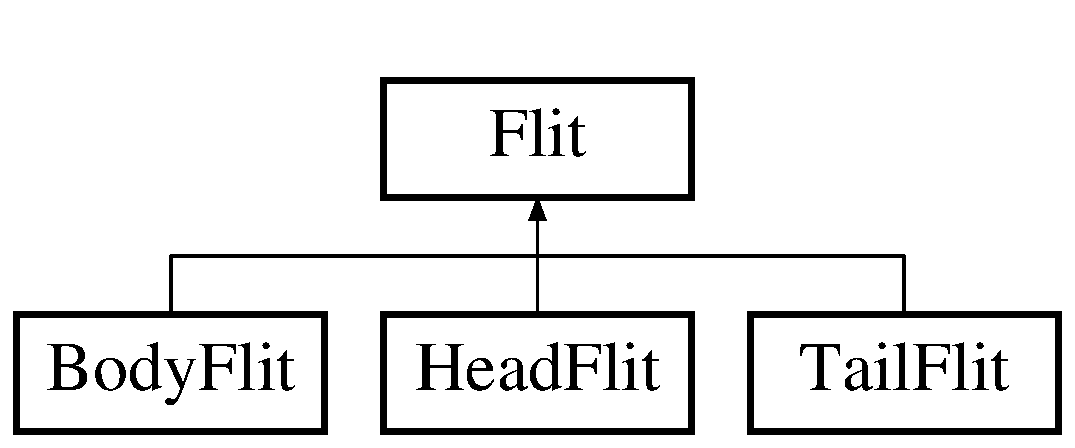
\includegraphics[height=2cm]{classFlit}
\end{center}
\end{figure}
\subsection*{Public Member Functions}
\begin{CompactItemize}
\item 
\hyperlink{classFlit_feebd85e6d981855d5405e163cb64f63}{Flit} ()
\item 
\hyperlink{classFlit_6c188313705a19f7fa7dffabb6591ceb}{$\sim$Flit} ()
\item 
void \hyperlink{classFlit_c290470e490b600742672da65d4b42f0}{populate\_\-phit\_\-data} (vector$<$ bool $>$ $\ast$c)
\item 
string \hyperlink{classFlit_ffc6c729a005389b51818aac59710dab}{toString} () const 
\end{CompactItemize}
\subsection*{Public Attributes}
\begin{CompactItemize}
\item 
vector$<$ \hyperlink{classPhit}{Phit} $>$ \hyperlink{classFlit_8f86afda1dc9b2393655bbabf7ebf42a}{phits}
\item 
\hyperlink{flit_8h_2c6c8cfc6307d086e578093535798328}{flit\_\-type} \hyperlink{classFlit_1a9a073876b8ac18b92e2b1b0eff33d7}{type}
\item 
\hyperlink{outputBuffer_8h_91ad9478d81a7aaf2593e8d9c3d06a14}{uint} \hyperlink{classFlit_784536ac677ec8b4f2924bd91fbfa4c2}{vc}
\end{CompactItemize}


\subsection{Constructor \& Destructor Documentation}
\hypertarget{classFlit_feebd85e6d981855d5405e163cb64f63}{
\index{Flit@{Flit}!Flit@{Flit}}
\index{Flit@{Flit}!Flit@{Flit}}
\subsubsection[{Flit}]{\setlength{\rightskip}{0pt plus 5cm}Flit::Flit ()}}
\label{classFlit_feebd85e6d981855d5405e163cb64f63}


\hypertarget{classFlit_6c188313705a19f7fa7dffabb6591ceb}{
\index{Flit@{Flit}!$\sim$Flit@{$\sim$Flit}}
\index{$\sim$Flit@{$\sim$Flit}!Flit@{Flit}}
\subsubsection[{$\sim$Flit}]{\setlength{\rightskip}{0pt plus 5cm}Flit::$\sim$Flit ()}}
\label{classFlit_6c188313705a19f7fa7dffabb6591ceb}




\subsection{Member Function Documentation}
\hypertarget{classFlit_c290470e490b600742672da65d4b42f0}{
\index{Flit@{Flit}!populate\_\-phit\_\-data@{populate\_\-phit\_\-data}}
\index{populate\_\-phit\_\-data@{populate\_\-phit\_\-data}!Flit@{Flit}}
\subsubsection[{populate\_\-phit\_\-data}]{\setlength{\rightskip}{0pt plus 5cm}void Flit::populate\_\-phit\_\-data (vector$<$ bool $>$ $\ast$ {\em c})}}
\label{classFlit_c290470e490b600742672da65d4b42f0}


\hypertarget{classFlit_ffc6c729a005389b51818aac59710dab}{
\index{Flit@{Flit}!toString@{toString}}
\index{toString@{toString}!Flit@{Flit}}
\subsubsection[{toString}]{\setlength{\rightskip}{0pt plus 5cm}string Flit::toString () const}}
\label{classFlit_ffc6c729a005389b51818aac59710dab}




Reimplemented in \hyperlink{classHeadFlit_4d22ac839cad2ac7ef0aedfeb54c9421}{HeadFlit}, \hyperlink{classBodyFlit_408f02aae1a229c761ff0f3537675cde}{BodyFlit}, and \hyperlink{classTailFlit_fb1c83457c5d834a8a859269154e3c4d}{TailFlit}.

\subsection{Member Data Documentation}
\hypertarget{classFlit_8f86afda1dc9b2393655bbabf7ebf42a}{
\index{Flit@{Flit}!phits@{phits}}
\index{phits@{phits}!Flit@{Flit}}
\subsubsection[{phits}]{\setlength{\rightskip}{0pt plus 5cm}vector$<${\bf Phit}$>$ {\bf Flit::phits}}}
\label{classFlit_8f86afda1dc9b2393655bbabf7ebf42a}


\hypertarget{classFlit_1a9a073876b8ac18b92e2b1b0eff33d7}{
\index{Flit@{Flit}!type@{type}}
\index{type@{type}!Flit@{Flit}}
\subsubsection[{type}]{\setlength{\rightskip}{0pt plus 5cm}{\bf flit\_\-type} {\bf Flit::type}}}
\label{classFlit_1a9a073876b8ac18b92e2b1b0eff33d7}


\hypertarget{classFlit_784536ac677ec8b4f2924bd91fbfa4c2}{
\index{Flit@{Flit}!vc@{vc}}
\index{vc@{vc}!Flit@{Flit}}
\subsubsection[{vc}]{\setlength{\rightskip}{0pt plus 5cm}{\bf uint} {\bf Flit::vc}}}
\label{classFlit_784536ac677ec8b4f2924bd91fbfa4c2}




The documentation for this class was generated from the following files:\begin{CompactItemize}
\item 
source/data\_\-types/impl/\hyperlink{flit_8h}{flit.h}\item 
source/data\_\-types/impl/\hyperlink{flit_8cc}{flit.cc}\end{CompactItemize}

\hypertarget{classGenericAddressDecoder}{
\section{GenericAddressDecoder Class Reference}
\label{classGenericAddressDecoder}\index{GenericAddressDecoder@{GenericAddressDecoder}}
}
{\tt \#include $<$genericAddressDecoder.h$>$}

\subsection*{Classes}
\begin{CompactItemize}
\item 
class \textbf{Address}
\end{CompactItemize}
\subsection*{Public Member Functions}
\begin{CompactItemize}
\item 
\hyperlink{classGenericAddressDecoder_c9f3d12b792ee1821499d4e332b52690}{GenericAddressDecoder} ()
\item 
\hyperlink{classGenericAddressDecoder_9d20e3a126b7aa5ec9865ee6a4e1a6eb}{$\sim$GenericAddressDecoder} ()
\item 
void \hyperlink{classGenericAddressDecoder_8a2cc1c7e48dbbf11b03c49a3ce3e1d9}{push} (\hyperlink{classFlit}{Flit} $\ast$f, unsigned int vc)
\item 
unsigned int \hyperlink{classGenericAddressDecoder_3bab82f615b42ee907d37a6f601bd527}{get\_\-output\_\-port} (unsigned int channel)
\item 
unsigned int \hyperlink{classGenericAddressDecoder_d7d7f4cb63e720fd70d886eb6d11e812}{speculate\_\-port} (\hyperlink{classFlit}{Flit} $\ast$f, unsigned int ch)
\item 
unsigned int \hyperlink{classGenericAddressDecoder_81457cd722fd50e8297078e0729ea6b5}{speculate\_\-channel} (\hyperlink{classFlit}{Flit} $\ast$f, unsigned int ch)
\item 
unsigned int \hyperlink{classGenericAddressDecoder_99bfff56c04910dd0e3e397f8168d489}{get\_\-virtual\_\-channel} (unsigned int ch)
\item 
void \hyperlink{classGenericAddressDecoder_8473f733b74bc46dbcda7a5a4cdd4420}{set\_\-no\_\-virtual\_\-channels} (unsigned int ch)
\item 
unsigned int \hyperlink{classGenericAddressDecoder_339ae939c2361faac88813f1af3ce796}{get\_\-no\_\-channels} ()
\item 
bool \hyperlink{classGenericAddressDecoder_c11da10c5593e9677c0a19b6dfea46d8}{is\_\-empty} ()
\item 
string \hyperlink{classGenericAddressDecoder_5b4395166709804b6dd9cb784bc45a1d}{toString} () const 
\end{CompactItemize}
\subsection*{Public Attributes}
\begin{CompactItemize}
\item 
\hyperlink{outputBuffer_8h_91ad9478d81a7aaf2593e8d9c3d06a14}{uint} \hyperlink{classGenericAddressDecoder_9b8fd8a1cc36e6ab4b398b2a9a4f74bd}{node\_\-ip}
\item 
\hyperlink{outputBuffer_8h_91ad9478d81a7aaf2593e8d9c3d06a14}{uint} \hyperlink{classGenericAddressDecoder_e4958f1eabb1f538cbfa4f49a70819ee}{address}
\item 
vector$<$ \hyperlink{outputBuffer_8h_91ad9478d81a7aaf2593e8d9c3d06a14}{uint} $>$ \hyperlink{classGenericAddressDecoder_7b34be1b61592aa81a59122776d35d0a}{grid\_\-xloc}
\item 
vector$<$ \hyperlink{outputBuffer_8h_91ad9478d81a7aaf2593e8d9c3d06a14}{uint} $>$ \hyperlink{classGenericAddressDecoder_1ba45f3ca9054494e325c9ab49b61da8}{grid\_\-yloc}
\end{CompactItemize}


\subsection{Constructor \& Destructor Documentation}
\hypertarget{classGenericAddressDecoder_c9f3d12b792ee1821499d4e332b52690}{
\index{GenericAddressDecoder@{GenericAddressDecoder}!GenericAddressDecoder@{GenericAddressDecoder}}
\index{GenericAddressDecoder@{GenericAddressDecoder}!GenericAddressDecoder@{GenericAddressDecoder}}
\subsubsection[{GenericAddressDecoder}]{\setlength{\rightskip}{0pt plus 5cm}GenericAddressDecoder::GenericAddressDecoder ()}}
\label{classGenericAddressDecoder_c9f3d12b792ee1821499d4e332b52690}


\hypertarget{classGenericAddressDecoder_9d20e3a126b7aa5ec9865ee6a4e1a6eb}{
\index{GenericAddressDecoder@{GenericAddressDecoder}!$\sim$GenericAddressDecoder@{$\sim$GenericAddressDecoder}}
\index{$\sim$GenericAddressDecoder@{$\sim$GenericAddressDecoder}!GenericAddressDecoder@{GenericAddressDecoder}}
\subsubsection[{$\sim$GenericAddressDecoder}]{\setlength{\rightskip}{0pt plus 5cm}GenericAddressDecoder::$\sim$GenericAddressDecoder ()\hspace{0.3cm}{\tt  \mbox{[}inline\mbox{]}}}}
\label{classGenericAddressDecoder_9d20e3a126b7aa5ec9865ee6a4e1a6eb}




\subsection{Member Function Documentation}
\hypertarget{classGenericAddressDecoder_339ae939c2361faac88813f1af3ce796}{
\index{GenericAddressDecoder@{GenericAddressDecoder}!get\_\-no\_\-channels@{get\_\-no\_\-channels}}
\index{get\_\-no\_\-channels@{get\_\-no\_\-channels}!GenericAddressDecoder@{GenericAddressDecoder}}
\subsubsection[{get\_\-no\_\-channels}]{\setlength{\rightskip}{0pt plus 5cm}{\bf uint} GenericAddressDecoder::get\_\-no\_\-channels ()}}
\label{classGenericAddressDecoder_339ae939c2361faac88813f1af3ce796}


\hypertarget{classGenericAddressDecoder_3bab82f615b42ee907d37a6f601bd527}{
\index{GenericAddressDecoder@{GenericAddressDecoder}!get\_\-output\_\-port@{get\_\-output\_\-port}}
\index{get\_\-output\_\-port@{get\_\-output\_\-port}!GenericAddressDecoder@{GenericAddressDecoder}}
\subsubsection[{get\_\-output\_\-port}]{\setlength{\rightskip}{0pt plus 5cm}{\bf uint} GenericAddressDecoder::get\_\-output\_\-port (unsigned int {\em channel})}}
\label{classGenericAddressDecoder_3bab82f615b42ee907d37a6f601bd527}


\hypertarget{classGenericAddressDecoder_99bfff56c04910dd0e3e397f8168d489}{
\index{GenericAddressDecoder@{GenericAddressDecoder}!get\_\-virtual\_\-channel@{get\_\-virtual\_\-channel}}
\index{get\_\-virtual\_\-channel@{get\_\-virtual\_\-channel}!GenericAddressDecoder@{GenericAddressDecoder}}
\subsubsection[{get\_\-virtual\_\-channel}]{\setlength{\rightskip}{0pt plus 5cm}{\bf uint} GenericAddressDecoder::get\_\-virtual\_\-channel (unsigned int {\em ch})}}
\label{classGenericAddressDecoder_99bfff56c04910dd0e3e397f8168d489}


\hypertarget{classGenericAddressDecoder_c11da10c5593e9677c0a19b6dfea46d8}{
\index{GenericAddressDecoder@{GenericAddressDecoder}!is\_\-empty@{is\_\-empty}}
\index{is\_\-empty@{is\_\-empty}!GenericAddressDecoder@{GenericAddressDecoder}}
\subsubsection[{is\_\-empty}]{\setlength{\rightskip}{0pt plus 5cm}bool GenericAddressDecoder::is\_\-empty ()}}
\label{classGenericAddressDecoder_c11da10c5593e9677c0a19b6dfea46d8}


\hypertarget{classGenericAddressDecoder_8a2cc1c7e48dbbf11b03c49a3ce3e1d9}{
\index{GenericAddressDecoder@{GenericAddressDecoder}!push@{push}}
\index{push@{push}!GenericAddressDecoder@{GenericAddressDecoder}}
\subsubsection[{push}]{\setlength{\rightskip}{0pt plus 5cm}void GenericAddressDecoder::push ({\bf Flit} $\ast$ {\em f}, \/  unsigned int {\em vc})}}
\label{classGenericAddressDecoder_8a2cc1c7e48dbbf11b03c49a3ce3e1d9}


\hypertarget{classGenericAddressDecoder_8473f733b74bc46dbcda7a5a4cdd4420}{
\index{GenericAddressDecoder@{GenericAddressDecoder}!set\_\-no\_\-virtual\_\-channels@{set\_\-no\_\-virtual\_\-channels}}
\index{set\_\-no\_\-virtual\_\-channels@{set\_\-no\_\-virtual\_\-channels}!GenericAddressDecoder@{GenericAddressDecoder}}
\subsubsection[{set\_\-no\_\-virtual\_\-channels}]{\setlength{\rightskip}{0pt plus 5cm}void GenericAddressDecoder::set\_\-no\_\-virtual\_\-channels (unsigned int {\em ch})}}
\label{classGenericAddressDecoder_8473f733b74bc46dbcda7a5a4cdd4420}


\hypertarget{classGenericAddressDecoder_81457cd722fd50e8297078e0729ea6b5}{
\index{GenericAddressDecoder@{GenericAddressDecoder}!speculate\_\-channel@{speculate\_\-channel}}
\index{speculate\_\-channel@{speculate\_\-channel}!GenericAddressDecoder@{GenericAddressDecoder}}
\subsubsection[{speculate\_\-channel}]{\setlength{\rightskip}{0pt plus 5cm}unsigned int GenericAddressDecoder::speculate\_\-channel ({\bf Flit} $\ast$ {\em f}, \/  unsigned int {\em ch})}}
\label{classGenericAddressDecoder_81457cd722fd50e8297078e0729ea6b5}


\hypertarget{classGenericAddressDecoder_d7d7f4cb63e720fd70d886eb6d11e812}{
\index{GenericAddressDecoder@{GenericAddressDecoder}!speculate\_\-port@{speculate\_\-port}}
\index{speculate\_\-port@{speculate\_\-port}!GenericAddressDecoder@{GenericAddressDecoder}}
\subsubsection[{speculate\_\-port}]{\setlength{\rightskip}{0pt plus 5cm}unsigned int GenericAddressDecoder::speculate\_\-port ({\bf Flit} $\ast$ {\em f}, \/  unsigned int {\em ch})}}
\label{classGenericAddressDecoder_d7d7f4cb63e720fd70d886eb6d11e812}


\hypertarget{classGenericAddressDecoder_5b4395166709804b6dd9cb784bc45a1d}{
\index{GenericAddressDecoder@{GenericAddressDecoder}!toString@{toString}}
\index{toString@{toString}!GenericAddressDecoder@{GenericAddressDecoder}}
\subsubsection[{toString}]{\setlength{\rightskip}{0pt plus 5cm}string GenericAddressDecoder::toString () const}}
\label{classGenericAddressDecoder_5b4395166709804b6dd9cb784bc45a1d}




\subsection{Member Data Documentation}
\hypertarget{classGenericAddressDecoder_e4958f1eabb1f538cbfa4f49a70819ee}{
\index{GenericAddressDecoder@{GenericAddressDecoder}!address@{address}}
\index{address@{address}!GenericAddressDecoder@{GenericAddressDecoder}}
\subsubsection[{address}]{\setlength{\rightskip}{0pt plus 5cm}{\bf uint} {\bf GenericAddressDecoder::address}}}
\label{classGenericAddressDecoder_e4958f1eabb1f538cbfa4f49a70819ee}


\hypertarget{classGenericAddressDecoder_7b34be1b61592aa81a59122776d35d0a}{
\index{GenericAddressDecoder@{GenericAddressDecoder}!grid\_\-xloc@{grid\_\-xloc}}
\index{grid\_\-xloc@{grid\_\-xloc}!GenericAddressDecoder@{GenericAddressDecoder}}
\subsubsection[{grid\_\-xloc}]{\setlength{\rightskip}{0pt plus 5cm}vector$<$ {\bf uint} $>$ {\bf GenericAddressDecoder::grid\_\-xloc}}}
\label{classGenericAddressDecoder_7b34be1b61592aa81a59122776d35d0a}


\hypertarget{classGenericAddressDecoder_1ba45f3ca9054494e325c9ab49b61da8}{
\index{GenericAddressDecoder@{GenericAddressDecoder}!grid\_\-yloc@{grid\_\-yloc}}
\index{grid\_\-yloc@{grid\_\-yloc}!GenericAddressDecoder@{GenericAddressDecoder}}
\subsubsection[{grid\_\-yloc}]{\setlength{\rightskip}{0pt plus 5cm}vector$<$ {\bf uint} $>$ {\bf GenericAddressDecoder::grid\_\-yloc}}}
\label{classGenericAddressDecoder_1ba45f3ca9054494e325c9ab49b61da8}


\hypertarget{classGenericAddressDecoder_9b8fd8a1cc36e6ab4b398b2a9a4f74bd}{
\index{GenericAddressDecoder@{GenericAddressDecoder}!node\_\-ip@{node\_\-ip}}
\index{node\_\-ip@{node\_\-ip}!GenericAddressDecoder@{GenericAddressDecoder}}
\subsubsection[{node\_\-ip}]{\setlength{\rightskip}{0pt plus 5cm}{\bf uint} {\bf GenericAddressDecoder::node\_\-ip}}}
\label{classGenericAddressDecoder_9b8fd8a1cc36e6ab4b398b2a9a4f74bd}




The documentation for this class was generated from the following files:\begin{CompactItemize}
\item 
source/components/none/\hyperlink{genericAddressDecoder_8h}{genericAddressDecoder.h}\item 
source/components/none/\hyperlink{genericAddressDecoder_8cc}{genericAddressDecoder.cc}\end{CompactItemize}

\hypertarget{classGenericArbiter}{
\section{GenericArbiter Class Reference}
\label{classGenericArbiter}\index{GenericArbiter@{GenericArbiter}}
}
{\tt \#include $<$genericArbiter.h$>$}

Inheritance diagram for GenericArbiter::\begin{figure}[H]
\begin{center}
\leavevmode
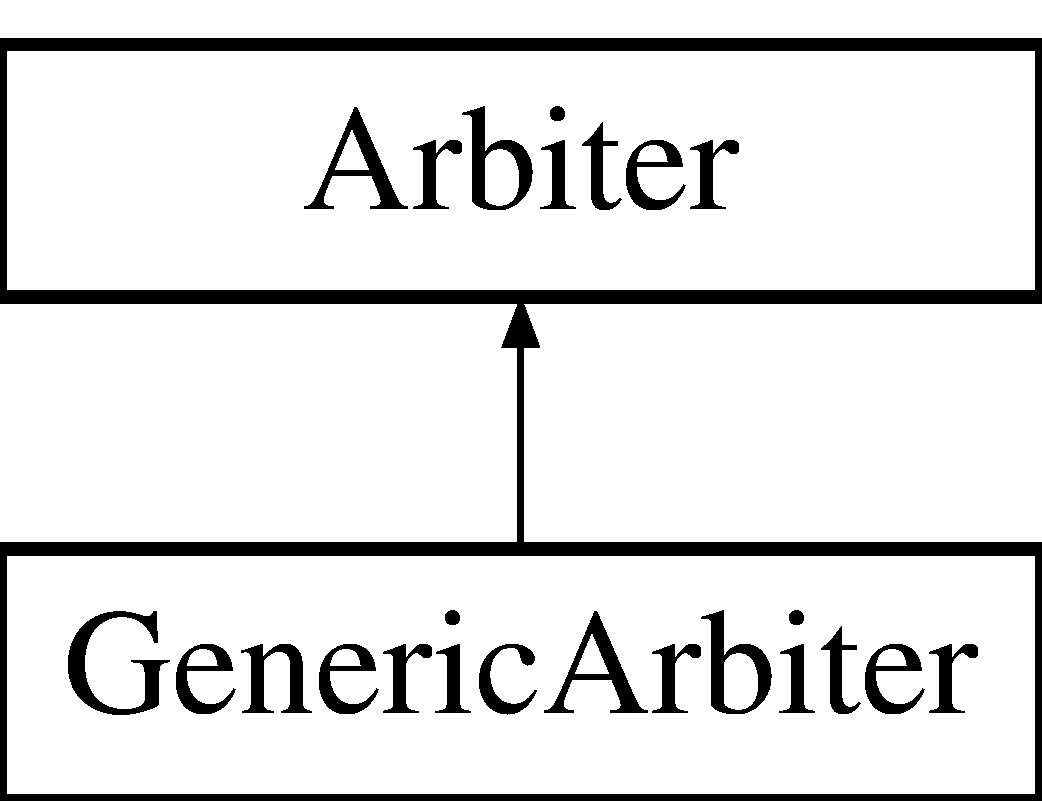
\includegraphics[height=2cm]{classGenericArbiter}
\end{center}
\end{figure}
\subsection*{Public Member Functions}
\begin{CompactItemize}
\item 
\hyperlink{classGenericArbiter_f268b17257b6084b8faa82e4539580f5}{GenericArbiter} ()
\item 
\hyperlink{classGenericArbiter_c8e72db9c3fb2c9b406933a104592519}{$\sim$GenericArbiter} ()
\item 
bool \hyperlink{classGenericArbiter_6cb1ab1819bd58fc51935af5af5bd6d5}{is\_\-requested} (\hyperlink{outputBuffer_8h_91ad9478d81a7aaf2593e8d9c3d06a14}{uint} ch)
\item 
void \hyperlink{classGenericArbiter_adbe3775870bfc27a5f57e37d73cec5b}{set\_\-req\_\-queue\_\-size} (\hyperlink{outputBuffer_8h_91ad9478d81a7aaf2593e8d9c3d06a14}{uint} size)
\item 
void \hyperlink{classGenericArbiter_2ecaad77822910dd7353c8c03f116690}{request} (\hyperlink{classFlit}{Flit} $\ast$f, \hyperlink{outputBuffer_8h_91ad9478d81a7aaf2593e8d9c3d06a14}{uint} index)
\item 
\hyperlink{classFlit}{Flit} $\ast$ \hyperlink{classGenericArbiter_16e40d95e115c183d604611c6e4c875c}{pull\_\-winner} ()
\item 
\hyperlink{outputBuffer_8h_91ad9478d81a7aaf2593e8d9c3d06a14}{uint} \hyperlink{classGenericArbiter_6f8e4f27cf748d7e73f3065d3d8beb2b}{get\_\-no\_\-requests} ()
\item 
\hyperlink{outputBuffer_8h_91ad9478d81a7aaf2593e8d9c3d06a14}{uint} \hyperlink{classGenericArbiter_4a5b38f3d16471a75c0c35fc1ecb3031}{pick\_\-winner} ()
\item 
\hyperlink{outputBuffer_8h_91ad9478d81a7aaf2593e8d9c3d06a14}{uint} \hyperlink{classGenericArbiter_d150c66feabc2154efea2fbad441cfc1}{pick\_\-winner} (vector$<$ bool $>$ ready)
\item 
void \hyperlink{classGenericArbiter_137758be6498b8dc717cf4d4c8bc56be}{clear\_\-winner} ()
\item 
bool \hyperlink{classGenericArbiter_bd1e990e713578e87719e634884effa6}{empty} ()
\item 
bool \hyperlink{classGenericArbiter_0e9396065d7b437fbac43768b3dfb7c1}{empty} (vector$<$ bool $>$ ready)
\item 
string \hyperlink{classGenericArbiter_dfd7645d22ce13eb428e73fd9fa34b63}{toString} () const 
\end{CompactItemize}
\subsection*{Public Attributes}
\begin{CompactItemize}
\item 
\hyperlink{outputBuffer_8h_91ad9478d81a7aaf2593e8d9c3d06a14}{uint} \hyperlink{classGenericArbiter_970eebd92edf4b43bd34dbe378aee0b4}{node\_\-ip}
\item 
\hyperlink{outputBuffer_8h_91ad9478d81a7aaf2593e8d9c3d06a14}{uint} \hyperlink{classGenericArbiter_d570be8e0435c540c11f46cd9e68d8fc}{address}
\item 
unsigned long long int \hyperlink{classGenericArbiter_c2b3b3256c40848d1e06cc15e15b7750}{write\_\-time}
\item 
vector$<$ \hyperlink{outputBuffer_8h_91ad9478d81a7aaf2593e8d9c3d06a14}{uint} $>$ \hyperlink{classGenericArbiter_2225ea6ef234e002fb69810552b02262}{next\_\-port}
\end{CompactItemize}


\subsection{Constructor \& Destructor Documentation}
\hypertarget{classGenericArbiter_f268b17257b6084b8faa82e4539580f5}{
\index{GenericArbiter@{GenericArbiter}!GenericArbiter@{GenericArbiter}}
\index{GenericArbiter@{GenericArbiter}!GenericArbiter@{GenericArbiter}}
\subsubsection[{GenericArbiter}]{\setlength{\rightskip}{0pt plus 5cm}GenericArbiter::GenericArbiter ()}}
\label{classGenericArbiter_f268b17257b6084b8faa82e4539580f5}


\hypertarget{classGenericArbiter_c8e72db9c3fb2c9b406933a104592519}{
\index{GenericArbiter@{GenericArbiter}!$\sim$GenericArbiter@{$\sim$GenericArbiter}}
\index{$\sim$GenericArbiter@{$\sim$GenericArbiter}!GenericArbiter@{GenericArbiter}}
\subsubsection[{$\sim$GenericArbiter}]{\setlength{\rightskip}{0pt plus 5cm}GenericArbiter::$\sim$GenericArbiter ()}}
\label{classGenericArbiter_c8e72db9c3fb2c9b406933a104592519}




\subsection{Member Function Documentation}
\hypertarget{classGenericArbiter_137758be6498b8dc717cf4d4c8bc56be}{
\index{GenericArbiter@{GenericArbiter}!clear\_\-winner@{clear\_\-winner}}
\index{clear\_\-winner@{clear\_\-winner}!GenericArbiter@{GenericArbiter}}
\subsubsection[{clear\_\-winner}]{\setlength{\rightskip}{0pt plus 5cm}void GenericArbiter::clear\_\-winner ()}}
\label{classGenericArbiter_137758be6498b8dc717cf4d4c8bc56be}


\hypertarget{classGenericArbiter_0e9396065d7b437fbac43768b3dfb7c1}{
\index{GenericArbiter@{GenericArbiter}!empty@{empty}}
\index{empty@{empty}!GenericArbiter@{GenericArbiter}}
\subsubsection[{empty}]{\setlength{\rightskip}{0pt plus 5cm}bool GenericArbiter::empty (vector$<$ bool $>$ {\em ready})}}
\label{classGenericArbiter_0e9396065d7b437fbac43768b3dfb7c1}


\hypertarget{classGenericArbiter_bd1e990e713578e87719e634884effa6}{
\index{GenericArbiter@{GenericArbiter}!empty@{empty}}
\index{empty@{empty}!GenericArbiter@{GenericArbiter}}
\subsubsection[{empty}]{\setlength{\rightskip}{0pt plus 5cm}bool GenericArbiter::empty ()}}
\label{classGenericArbiter_bd1e990e713578e87719e634884effa6}


\hypertarget{classGenericArbiter_6f8e4f27cf748d7e73f3065d3d8beb2b}{
\index{GenericArbiter@{GenericArbiter}!get\_\-no\_\-requests@{get\_\-no\_\-requests}}
\index{get\_\-no\_\-requests@{get\_\-no\_\-requests}!GenericArbiter@{GenericArbiter}}
\subsubsection[{get\_\-no\_\-requests}]{\setlength{\rightskip}{0pt plus 5cm}{\bf uint} GenericArbiter::get\_\-no\_\-requests ()}}
\label{classGenericArbiter_6f8e4f27cf748d7e73f3065d3d8beb2b}


\hypertarget{classGenericArbiter_6cb1ab1819bd58fc51935af5af5bd6d5}{
\index{GenericArbiter@{GenericArbiter}!is\_\-requested@{is\_\-requested}}
\index{is\_\-requested@{is\_\-requested}!GenericArbiter@{GenericArbiter}}
\subsubsection[{is\_\-requested}]{\setlength{\rightskip}{0pt plus 5cm}bool GenericArbiter::is\_\-requested ({\bf uint} {\em ch})}}
\label{classGenericArbiter_6cb1ab1819bd58fc51935af5af5bd6d5}


\hypertarget{classGenericArbiter_d150c66feabc2154efea2fbad441cfc1}{
\index{GenericArbiter@{GenericArbiter}!pick\_\-winner@{pick\_\-winner}}
\index{pick\_\-winner@{pick\_\-winner}!GenericArbiter@{GenericArbiter}}
\subsubsection[{pick\_\-winner}]{\setlength{\rightskip}{0pt plus 5cm}{\bf uint} GenericArbiter::pick\_\-winner (vector$<$ bool $>$ {\em ready})}}
\label{classGenericArbiter_d150c66feabc2154efea2fbad441cfc1}


\hypertarget{classGenericArbiter_4a5b38f3d16471a75c0c35fc1ecb3031}{
\index{GenericArbiter@{GenericArbiter}!pick\_\-winner@{pick\_\-winner}}
\index{pick\_\-winner@{pick\_\-winner}!GenericArbiter@{GenericArbiter}}
\subsubsection[{pick\_\-winner}]{\setlength{\rightskip}{0pt plus 5cm}{\bf uint} GenericArbiter::pick\_\-winner ()}}
\label{classGenericArbiter_4a5b38f3d16471a75c0c35fc1ecb3031}


\hypertarget{classGenericArbiter_16e40d95e115c183d604611c6e4c875c}{
\index{GenericArbiter@{GenericArbiter}!pull\_\-winner@{pull\_\-winner}}
\index{pull\_\-winner@{pull\_\-winner}!GenericArbiter@{GenericArbiter}}
\subsubsection[{pull\_\-winner}]{\setlength{\rightskip}{0pt plus 5cm}{\bf Flit} $\ast$ GenericArbiter::pull\_\-winner ()}}
\label{classGenericArbiter_16e40d95e115c183d604611c6e4c875c}


\hypertarget{classGenericArbiter_2ecaad77822910dd7353c8c03f116690}{
\index{GenericArbiter@{GenericArbiter}!request@{request}}
\index{request@{request}!GenericArbiter@{GenericArbiter}}
\subsubsection[{request}]{\setlength{\rightskip}{0pt plus 5cm}void GenericArbiter::request ({\bf Flit} $\ast$ {\em f}, \/  {\bf uint} {\em index})}}
\label{classGenericArbiter_2ecaad77822910dd7353c8c03f116690}


\hypertarget{classGenericArbiter_adbe3775870bfc27a5f57e37d73cec5b}{
\index{GenericArbiter@{GenericArbiter}!set\_\-req\_\-queue\_\-size@{set\_\-req\_\-queue\_\-size}}
\index{set\_\-req\_\-queue\_\-size@{set\_\-req\_\-queue\_\-size}!GenericArbiter@{GenericArbiter}}
\subsubsection[{set\_\-req\_\-queue\_\-size}]{\setlength{\rightskip}{0pt plus 5cm}void GenericArbiter::set\_\-req\_\-queue\_\-size ({\bf uint} {\em size})}}
\label{classGenericArbiter_adbe3775870bfc27a5f57e37d73cec5b}


\hypertarget{classGenericArbiter_dfd7645d22ce13eb428e73fd9fa34b63}{
\index{GenericArbiter@{GenericArbiter}!toString@{toString}}
\index{toString@{toString}!GenericArbiter@{GenericArbiter}}
\subsubsection[{toString}]{\setlength{\rightskip}{0pt plus 5cm}string GenericArbiter::toString () const}}
\label{classGenericArbiter_dfd7645d22ce13eb428e73fd9fa34b63}




\subsection{Member Data Documentation}
\hypertarget{classGenericArbiter_d570be8e0435c540c11f46cd9e68d8fc}{
\index{GenericArbiter@{GenericArbiter}!address@{address}}
\index{address@{address}!GenericArbiter@{GenericArbiter}}
\subsubsection[{address}]{\setlength{\rightskip}{0pt plus 5cm}{\bf uint} {\bf GenericArbiter::address}}}
\label{classGenericArbiter_d570be8e0435c540c11f46cd9e68d8fc}


\hypertarget{classGenericArbiter_2225ea6ef234e002fb69810552b02262}{
\index{GenericArbiter@{GenericArbiter}!next\_\-port@{next\_\-port}}
\index{next\_\-port@{next\_\-port}!GenericArbiter@{GenericArbiter}}
\subsubsection[{next\_\-port}]{\setlength{\rightskip}{0pt plus 5cm}vector$<${\bf uint} $>$ {\bf GenericArbiter::next\_\-port}}}
\label{classGenericArbiter_2225ea6ef234e002fb69810552b02262}


\hypertarget{classGenericArbiter_970eebd92edf4b43bd34dbe378aee0b4}{
\index{GenericArbiter@{GenericArbiter}!node\_\-ip@{node\_\-ip}}
\index{node\_\-ip@{node\_\-ip}!GenericArbiter@{GenericArbiter}}
\subsubsection[{node\_\-ip}]{\setlength{\rightskip}{0pt plus 5cm}{\bf uint} {\bf GenericArbiter::node\_\-ip}}}
\label{classGenericArbiter_970eebd92edf4b43bd34dbe378aee0b4}


\hypertarget{classGenericArbiter_c2b3b3256c40848d1e06cc15e15b7750}{
\index{GenericArbiter@{GenericArbiter}!write\_\-time@{write\_\-time}}
\index{write\_\-time@{write\_\-time}!GenericArbiter@{GenericArbiter}}
\subsubsection[{write\_\-time}]{\setlength{\rightskip}{0pt plus 5cm}unsigned long long int {\bf GenericArbiter::write\_\-time}}}
\label{classGenericArbiter_c2b3b3256c40848d1e06cc15e15b7750}




The documentation for this class was generated from the following files:\begin{CompactItemize}
\item 
source/components/none/\hyperlink{genericArbiter_8h}{genericArbiter.h}\item 
source/components/none/\hyperlink{genericArbiter_8cc}{genericArbiter.cc}\end{CompactItemize}

\hypertarget{classGenericBuffer}{
\section{GenericBuffer Class Reference}
\label{classGenericBuffer}\index{GenericBuffer@{GenericBuffer}}
}
{\tt \#include $<$genericBuffer.h$>$}

Inheritance diagram for GenericBuffer::\begin{figure}[H]
\begin{center}
\leavevmode
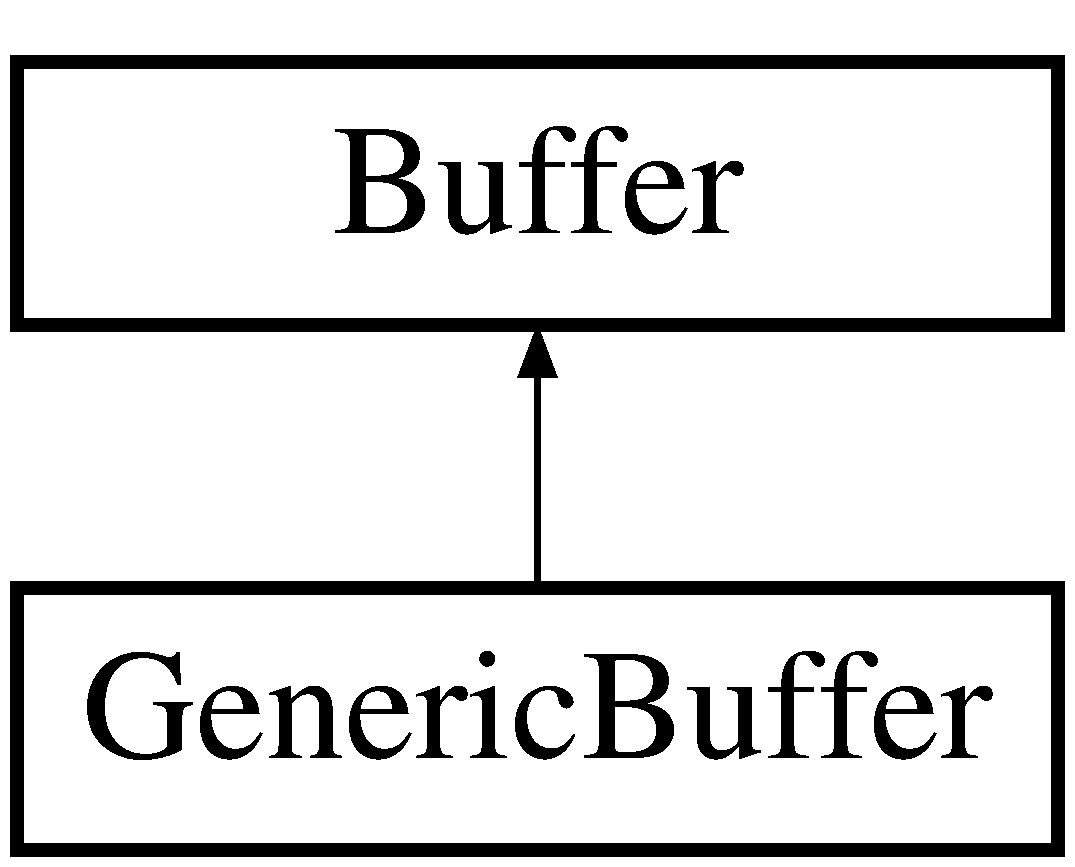
\includegraphics[height=2cm]{classGenericBuffer}
\end{center}
\end{figure}
\subsection*{Public Member Functions}
\begin{CompactItemize}
\item 
\hyperlink{classGenericBuffer_4281e7a40133d057f6cfad3b715084b0}{GenericBuffer} ()
\item 
\hyperlink{classGenericBuffer_d9a4c588a03bdf24a6fe586376d17e0c}{$\sim$GenericBuffer} ()
\item 
void \hyperlink{classGenericBuffer_c5a0781106485f9567898b49021f6346}{push} (\hyperlink{classFlit}{Flit} $\ast$f)
\item 
\hyperlink{classFlit}{Flit} $\ast$ \hyperlink{classGenericBuffer_6ce6f151eb6f65ec1fffafffb04a8f0e}{pull} ()
\item 
\hyperlink{outputBuffer_8h_91ad9478d81a7aaf2593e8d9c3d06a14}{uint} \hyperlink{classGenericBuffer_f2f85cf979616bab9dad5373d25d7813}{get\_\-occupancy} (\hyperlink{outputBuffer_8h_91ad9478d81a7aaf2593e8d9c3d06a14}{uint} ch) const 
\item 
void \hyperlink{classGenericBuffer_d2b0822ec5f56ebea495b19562028f4c}{resize} (\hyperlink{outputBuffer_8h_91ad9478d81a7aaf2593e8d9c3d06a14}{uint} vcs, \hyperlink{outputBuffer_8h_91ad9478d81a7aaf2593e8d9c3d06a14}{uint} buffer\_\-size)
\item 
\hyperlink{outputBuffer_8h_91ad9478d81a7aaf2593e8d9c3d06a14}{uint} \hyperlink{classGenericBuffer_528c7b73ffbb3870cab0fc999a01a024}{get\_\-no\_\-vcs} () const 
\item 
void \hyperlink{classGenericBuffer_6d7fe4a638dc7eb0358c3490bf8d2cf4}{change\_\-pull\_\-channel} (\hyperlink{outputBuffer_8h_91ad9478d81a7aaf2593e8d9c3d06a14}{uint} ch)
\item 
void \hyperlink{classGenericBuffer_31e2c8b678d219fcc5d6e351f2f8623c}{change\_\-push\_\-channel} (\hyperlink{outputBuffer_8h_91ad9478d81a7aaf2593e8d9c3d06a14}{uint} ch)
\item 
\hyperlink{outputBuffer_8h_91ad9478d81a7aaf2593e8d9c3d06a14}{uint} \hyperlink{classGenericBuffer_3e87475edf8151591ef57f9ca4cd9a25}{get\_\-pull\_\-channel} () const 
\item 
\hyperlink{outputBuffer_8h_91ad9478d81a7aaf2593e8d9c3d06a14}{uint} \hyperlink{classGenericBuffer_3b5ed41f7cee8ba1fa059aaa0b9db55a}{get\_\-push\_\-channel} () const 
\item 
bool \hyperlink{classGenericBuffer_91aa6e2af039aa6c1a50a599fc3f3203}{is\_\-channel\_\-full} (\hyperlink{outputBuffer_8h_91ad9478d81a7aaf2593e8d9c3d06a14}{uint} ch) const 
\item 
bool \hyperlink{classGenericBuffer_94742936925e0b4873dd270aed2c326d}{is\_\-empty} (\hyperlink{outputBuffer_8h_91ad9478d81a7aaf2593e8d9c3d06a14}{uint} ch) const 
\item 
string \hyperlink{classGenericBuffer_3e9808bf28490fcc38ba13e7eb6ef501}{toString} () const 
\item 
void \hyperlink{classGenericBuffer_61f0e9249ca38d149372bdd74906f2a7}{got\_\-credit} (\hyperlink{outputBuffer_8h_91ad9478d81a7aaf2593e8d9c3d06a14}{uint} ch)
\item 
\hyperlink{outputBuffer_8h_91ad9478d81a7aaf2593e8d9c3d06a14}{uint} \hyperlink{classGenericBuffer_8c80e28741bae248ed61c72cc5399f2d}{get\_\-no\_\-credits} (\hyperlink{outputBuffer_8h_91ad9478d81a7aaf2593e8d9c3d06a14}{uint} ch) const 
\item 
void \hyperlink{classGenericBuffer_222b1ccd9db0a123acb9f3d34d38881c}{set\_\-no\_\-credits} (\hyperlink{outputBuffer_8h_91ad9478d81a7aaf2593e8d9c3d06a14}{uint} no)
\end{CompactItemize}
\subsection*{Public Attributes}
\begin{CompactItemize}
\item 
vector$<$ queue$<$ \hyperlink{classFlit}{Flit} $\ast$ $>$ $>$ \hyperlink{classGenericBuffer_827e77b8ad0d8fcd36c95e63b6ed8001}{buffers}
\item 
vector$<$ int $>$ \hyperlink{classGenericBuffer_10b8e8d2522ed4797fa485d6ffa41838}{next\_\-port}
\end{CompactItemize}


\subsection{Constructor \& Destructor Documentation}
\hypertarget{classGenericBuffer_4281e7a40133d057f6cfad3b715084b0}{
\index{GenericBuffer@{GenericBuffer}!GenericBuffer@{GenericBuffer}}
\index{GenericBuffer@{GenericBuffer}!GenericBuffer@{GenericBuffer}}
\subsubsection[{GenericBuffer}]{\setlength{\rightskip}{0pt plus 5cm}GenericBuffer::GenericBuffer ()}}
\label{classGenericBuffer_4281e7a40133d057f6cfad3b715084b0}


\hypertarget{classGenericBuffer_d9a4c588a03bdf24a6fe586376d17e0c}{
\index{GenericBuffer@{GenericBuffer}!$\sim$GenericBuffer@{$\sim$GenericBuffer}}
\index{$\sim$GenericBuffer@{$\sim$GenericBuffer}!GenericBuffer@{GenericBuffer}}
\subsubsection[{$\sim$GenericBuffer}]{\setlength{\rightskip}{0pt plus 5cm}GenericBuffer::$\sim$GenericBuffer ()}}
\label{classGenericBuffer_d9a4c588a03bdf24a6fe586376d17e0c}




\subsection{Member Function Documentation}
\hypertarget{classGenericBuffer_6d7fe4a638dc7eb0358c3490bf8d2cf4}{
\index{GenericBuffer@{GenericBuffer}!change\_\-pull\_\-channel@{change\_\-pull\_\-channel}}
\index{change\_\-pull\_\-channel@{change\_\-pull\_\-channel}!GenericBuffer@{GenericBuffer}}
\subsubsection[{change\_\-pull\_\-channel}]{\setlength{\rightskip}{0pt plus 5cm}void GenericBuffer::change\_\-pull\_\-channel ({\bf uint} {\em ch})}}
\label{classGenericBuffer_6d7fe4a638dc7eb0358c3490bf8d2cf4}


\hypertarget{classGenericBuffer_31e2c8b678d219fcc5d6e351f2f8623c}{
\index{GenericBuffer@{GenericBuffer}!change\_\-push\_\-channel@{change\_\-push\_\-channel}}
\index{change\_\-push\_\-channel@{change\_\-push\_\-channel}!GenericBuffer@{GenericBuffer}}
\subsubsection[{change\_\-push\_\-channel}]{\setlength{\rightskip}{0pt plus 5cm}void GenericBuffer::change\_\-push\_\-channel ({\bf uint} {\em ch})}}
\label{classGenericBuffer_31e2c8b678d219fcc5d6e351f2f8623c}


\hypertarget{classGenericBuffer_8c80e28741bae248ed61c72cc5399f2d}{
\index{GenericBuffer@{GenericBuffer}!get\_\-no\_\-credits@{get\_\-no\_\-credits}}
\index{get\_\-no\_\-credits@{get\_\-no\_\-credits}!GenericBuffer@{GenericBuffer}}
\subsubsection[{get\_\-no\_\-credits}]{\setlength{\rightskip}{0pt plus 5cm}{\bf uint} GenericBuffer::get\_\-no\_\-credits ({\bf uint} {\em ch}) const}}
\label{classGenericBuffer_8c80e28741bae248ed61c72cc5399f2d}


\hypertarget{classGenericBuffer_528c7b73ffbb3870cab0fc999a01a024}{
\index{GenericBuffer@{GenericBuffer}!get\_\-no\_\-vcs@{get\_\-no\_\-vcs}}
\index{get\_\-no\_\-vcs@{get\_\-no\_\-vcs}!GenericBuffer@{GenericBuffer}}
\subsubsection[{get\_\-no\_\-vcs}]{\setlength{\rightskip}{0pt plus 5cm}{\bf uint} GenericBuffer::get\_\-no\_\-vcs () const}}
\label{classGenericBuffer_528c7b73ffbb3870cab0fc999a01a024}


\hypertarget{classGenericBuffer_f2f85cf979616bab9dad5373d25d7813}{
\index{GenericBuffer@{GenericBuffer}!get\_\-occupancy@{get\_\-occupancy}}
\index{get\_\-occupancy@{get\_\-occupancy}!GenericBuffer@{GenericBuffer}}
\subsubsection[{get\_\-occupancy}]{\setlength{\rightskip}{0pt plus 5cm}{\bf uint} GenericBuffer::get\_\-occupancy ({\bf uint} {\em ch}) const\hspace{0.3cm}{\tt  \mbox{[}virtual\mbox{]}}}}
\label{classGenericBuffer_f2f85cf979616bab9dad5373d25d7813}




Implements \hyperlink{classBuffer_af4e2d4031945429ae58350b5897570a}{Buffer}.\hypertarget{classGenericBuffer_3e87475edf8151591ef57f9ca4cd9a25}{
\index{GenericBuffer@{GenericBuffer}!get\_\-pull\_\-channel@{get\_\-pull\_\-channel}}
\index{get\_\-pull\_\-channel@{get\_\-pull\_\-channel}!GenericBuffer@{GenericBuffer}}
\subsubsection[{get\_\-pull\_\-channel}]{\setlength{\rightskip}{0pt plus 5cm}{\bf uint} GenericBuffer::get\_\-pull\_\-channel () const}}
\label{classGenericBuffer_3e87475edf8151591ef57f9ca4cd9a25}


\hypertarget{classGenericBuffer_3b5ed41f7cee8ba1fa059aaa0b9db55a}{
\index{GenericBuffer@{GenericBuffer}!get\_\-push\_\-channel@{get\_\-push\_\-channel}}
\index{get\_\-push\_\-channel@{get\_\-push\_\-channel}!GenericBuffer@{GenericBuffer}}
\subsubsection[{get\_\-push\_\-channel}]{\setlength{\rightskip}{0pt plus 5cm}{\bf uint} GenericBuffer::get\_\-push\_\-channel () const}}
\label{classGenericBuffer_3b5ed41f7cee8ba1fa059aaa0b9db55a}


\hypertarget{classGenericBuffer_61f0e9249ca38d149372bdd74906f2a7}{
\index{GenericBuffer@{GenericBuffer}!got\_\-credit@{got\_\-credit}}
\index{got\_\-credit@{got\_\-credit}!GenericBuffer@{GenericBuffer}}
\subsubsection[{got\_\-credit}]{\setlength{\rightskip}{0pt plus 5cm}void GenericBuffer::got\_\-credit ({\bf uint} {\em ch})}}
\label{classGenericBuffer_61f0e9249ca38d149372bdd74906f2a7}


\hypertarget{classGenericBuffer_91aa6e2af039aa6c1a50a599fc3f3203}{
\index{GenericBuffer@{GenericBuffer}!is\_\-channel\_\-full@{is\_\-channel\_\-full}}
\index{is\_\-channel\_\-full@{is\_\-channel\_\-full}!GenericBuffer@{GenericBuffer}}
\subsubsection[{is\_\-channel\_\-full}]{\setlength{\rightskip}{0pt plus 5cm}bool GenericBuffer::is\_\-channel\_\-full ({\bf uint} {\em ch}) const}}
\label{classGenericBuffer_91aa6e2af039aa6c1a50a599fc3f3203}


\hypertarget{classGenericBuffer_94742936925e0b4873dd270aed2c326d}{
\index{GenericBuffer@{GenericBuffer}!is\_\-empty@{is\_\-empty}}
\index{is\_\-empty@{is\_\-empty}!GenericBuffer@{GenericBuffer}}
\subsubsection[{is\_\-empty}]{\setlength{\rightskip}{0pt plus 5cm}bool GenericBuffer::is\_\-empty ({\bf uint} {\em ch}) const}}
\label{classGenericBuffer_94742936925e0b4873dd270aed2c326d}


\hypertarget{classGenericBuffer_6ce6f151eb6f65ec1fffafffb04a8f0e}{
\index{GenericBuffer@{GenericBuffer}!pull@{pull}}
\index{pull@{pull}!GenericBuffer@{GenericBuffer}}
\subsubsection[{pull}]{\setlength{\rightskip}{0pt plus 5cm}{\bf Flit} $\ast$ GenericBuffer::pull ()\hspace{0.3cm}{\tt  \mbox{[}virtual\mbox{]}}}}
\label{classGenericBuffer_6ce6f151eb6f65ec1fffafffb04a8f0e}




Implements \hyperlink{classBuffer_95f5c230f9c261bc13ddcfafcc340e7e}{Buffer}.\hypertarget{classGenericBuffer_c5a0781106485f9567898b49021f6346}{
\index{GenericBuffer@{GenericBuffer}!push@{push}}
\index{push@{push}!GenericBuffer@{GenericBuffer}}
\subsubsection[{push}]{\setlength{\rightskip}{0pt plus 5cm}void GenericBuffer::push ({\bf Flit} $\ast$ {\em f})\hspace{0.3cm}{\tt  \mbox{[}virtual\mbox{]}}}}
\label{classGenericBuffer_c5a0781106485f9567898b49021f6346}




Implements \hyperlink{classBuffer_c9dce1860c655146f000df30314caaa9}{Buffer}.\hypertarget{classGenericBuffer_d2b0822ec5f56ebea495b19562028f4c}{
\index{GenericBuffer@{GenericBuffer}!resize@{resize}}
\index{resize@{resize}!GenericBuffer@{GenericBuffer}}
\subsubsection[{resize}]{\setlength{\rightskip}{0pt plus 5cm}void GenericBuffer::resize ({\bf uint} {\em vcs}, \/  {\bf uint} {\em buffer\_\-size})}}
\label{classGenericBuffer_d2b0822ec5f56ebea495b19562028f4c}


\hypertarget{classGenericBuffer_222b1ccd9db0a123acb9f3d34d38881c}{
\index{GenericBuffer@{GenericBuffer}!set\_\-no\_\-credits@{set\_\-no\_\-credits}}
\index{set\_\-no\_\-credits@{set\_\-no\_\-credits}!GenericBuffer@{GenericBuffer}}
\subsubsection[{set\_\-no\_\-credits}]{\setlength{\rightskip}{0pt plus 5cm}void GenericBuffer::set\_\-no\_\-credits ({\bf uint} {\em no})}}
\label{classGenericBuffer_222b1ccd9db0a123acb9f3d34d38881c}


\hypertarget{classGenericBuffer_3e9808bf28490fcc38ba13e7eb6ef501}{
\index{GenericBuffer@{GenericBuffer}!toString@{toString}}
\index{toString@{toString}!GenericBuffer@{GenericBuffer}}
\subsubsection[{toString}]{\setlength{\rightskip}{0pt plus 5cm}string GenericBuffer::toString () const}}
\label{classGenericBuffer_3e9808bf28490fcc38ba13e7eb6ef501}




\subsection{Member Data Documentation}
\hypertarget{classGenericBuffer_827e77b8ad0d8fcd36c95e63b6ed8001}{
\index{GenericBuffer@{GenericBuffer}!buffers@{buffers}}
\index{buffers@{buffers}!GenericBuffer@{GenericBuffer}}
\subsubsection[{buffers}]{\setlength{\rightskip}{0pt plus 5cm}vector$<$ queue$<${\bf Flit}$\ast$$>$ $>$ {\bf GenericBuffer::buffers}}}
\label{classGenericBuffer_827e77b8ad0d8fcd36c95e63b6ed8001}


\hypertarget{classGenericBuffer_10b8e8d2522ed4797fa485d6ffa41838}{
\index{GenericBuffer@{GenericBuffer}!next\_\-port@{next\_\-port}}
\index{next\_\-port@{next\_\-port}!GenericBuffer@{GenericBuffer}}
\subsubsection[{next\_\-port}]{\setlength{\rightskip}{0pt plus 5cm}vector$<$ int $>$ {\bf GenericBuffer::next\_\-port}}}
\label{classGenericBuffer_10b8e8d2522ed4797fa485d6ffa41838}




The documentation for this class was generated from the following files:\begin{CompactItemize}
\item 
source/components/impl/\hyperlink{impl_2genericBuffer_8h}{genericBuffer.h}\item 
source/components/impl/\hyperlink{impl_2genericBuffer_8cc}{genericBuffer.cc}\end{CompactItemize}

\hypertarget{classGenericCrossbar}{
\section{GenericCrossbar Class Reference}
\label{classGenericCrossbar}\index{GenericCrossbar@{GenericCrossbar}}
}
{\tt \#include $<$genericCrossbar.h$>$}

Inheritance diagram for GenericCrossbar::\begin{figure}[H]
\begin{center}
\leavevmode
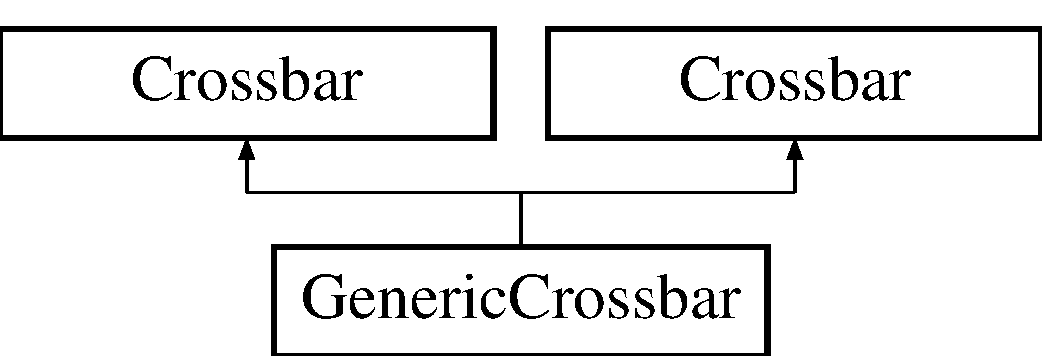
\includegraphics[height=2cm]{classGenericCrossbar}
\end{center}
\end{figure}
\subsection*{Classes}
\begin{CompactItemize}
\item 
class \textbf{CrossbarUnit}
\end{CompactItemize}
\subsection*{Public Member Functions}
\begin{CompactItemize}
\item 
\hyperlink{classGenericCrossbar_4a686c329c66490d847cc938b7e02aae}{GenericCrossbar} ()
\item 
\hyperlink{classGenericCrossbar_53c13d3c966feb35331958f7a2f9f90c}{$\sim$GenericCrossbar} ()
\item 
void \hyperlink{classGenericCrossbar_c97249405a9bc78f2c1c9c28ad660472}{set\_\-input\_\-ports} (\hyperlink{outputBuffer_8h_91ad9478d81a7aaf2593e8d9c3d06a14}{uint} ports)
\item 
void \hyperlink{classGenericCrossbar_5b9a2875ec8a1bb19683304ae31e3364}{set\_\-output\_\-ports} (\hyperlink{outputBuffer_8h_91ad9478d81a7aaf2593e8d9c3d06a14}{uint} ports)
\item 
\hyperlink{outputBuffer_8h_91ad9478d81a7aaf2593e8d9c3d06a14}{uint} \hyperlink{classGenericCrossbar_8758e38060de9899fa70ad069b83e9fc}{get\_\-no\_\-input\_\-ports} ()
\item 
\hyperlink{outputBuffer_8h_91ad9478d81a7aaf2593e8d9c3d06a14}{uint} \hyperlink{classGenericCrossbar_6ca09eb5520228b39d718e3994a5b84f}{get\_\-no\_\-output\_\-ports} ()
\item 
void \hyperlink{classGenericCrossbar_e9d67e36be87ea3169baa80ae52044e3}{set\_\-no\_\-virtual\_\-channels} (\hyperlink{outputBuffer_8h_91ad9478d81a7aaf2593e8d9c3d06a14}{uint} no)
\item 
\hyperlink{outputBuffer_8h_91ad9478d81a7aaf2593e8d9c3d06a14}{uint} \hyperlink{classGenericCrossbar_945a3d32809787bd2c5ee68714467467}{get\_\-no\_\-channels} ()
\item 
\hyperlink{outputBuffer_8h_91ad9478d81a7aaf2593e8d9c3d06a14}{uint} \hyperlink{classGenericCrossbar_65b435392191561b7a4759e20aacab4e}{get\_\-map} (\hyperlink{outputBuffer_8h_91ad9478d81a7aaf2593e8d9c3d06a14}{uint} in\_\-port, \hyperlink{outputBuffer_8h_91ad9478d81a7aaf2593e8d9c3d06a14}{uint} ch)
\item 
void \hyperlink{classGenericCrossbar_50c8203133960f74f6d82649b0c864be}{configure\_\-crossbar} (\hyperlink{outputBuffer_8h_91ad9478d81a7aaf2593e8d9c3d06a14}{uint} in\_\-port, \hyperlink{outputBuffer_8h_91ad9478d81a7aaf2593e8d9c3d06a14}{uint} out\_\-port, \hyperlink{outputBuffer_8h_91ad9478d81a7aaf2593e8d9c3d06a14}{uint} ch)
\item 
void \hyperlink{classGenericCrossbar_d925d4a2c3b5b4585e087dc423eeb0b8}{push} (\hyperlink{outputBuffer_8h_91ad9478d81a7aaf2593e8d9c3d06a14}{uint} in\_\-port, \hyperlink{outputBuffer_8h_91ad9478d81a7aaf2593e8d9c3d06a14}{uint} ch)
\item 
void \hyperlink{classGenericCrossbar_3c3fa82ff5db189ec69497f79e15112c}{pull} (\hyperlink{outputBuffer_8h_91ad9478d81a7aaf2593e8d9c3d06a14}{uint} out\_\-port, \hyperlink{outputBuffer_8h_91ad9478d81a7aaf2593e8d9c3d06a14}{uint} ch)
\item 
bool \hyperlink{classGenericCrossbar_1949b9db3b5b1950ad6a2c9e46103024}{is\_\-full} (\hyperlink{outputBuffer_8h_91ad9478d81a7aaf2593e8d9c3d06a14}{uint} in\_\-port, \hyperlink{outputBuffer_8h_91ad9478d81a7aaf2593e8d9c3d06a14}{uint} ch)
\item 
bool \hyperlink{classGenericCrossbar_b1dc236c4543805ac9fd50f25adcc27e}{is\_\-empty} (\hyperlink{outputBuffer_8h_91ad9478d81a7aaf2593e8d9c3d06a14}{uint} out\_\-port, \hyperlink{outputBuffer_8h_91ad9478d81a7aaf2593e8d9c3d06a14}{uint} ch)
\item 
string \hyperlink{classGenericCrossbar_6794211c84eda89c8ff8e2460d5201fc}{toString} () const 
\item 
\hyperlink{classGenericCrossbar_4a686c329c66490d847cc938b7e02aae}{GenericCrossbar} ()
\item 
\hyperlink{classGenericCrossbar_53c13d3c966feb35331958f7a2f9f90c}{$\sim$GenericCrossbar} ()
\item 
void \hyperlink{classGenericCrossbar_c97249405a9bc78f2c1c9c28ad660472}{set\_\-input\_\-ports} (\hyperlink{outputBuffer_8h_91ad9478d81a7aaf2593e8d9c3d06a14}{uint} ports)
\item 
void \hyperlink{classGenericCrossbar_5b9a2875ec8a1bb19683304ae31e3364}{set\_\-output\_\-ports} (\hyperlink{outputBuffer_8h_91ad9478d81a7aaf2593e8d9c3d06a14}{uint} ports)
\item 
\hyperlink{outputBuffer_8h_91ad9478d81a7aaf2593e8d9c3d06a14}{uint} \hyperlink{classGenericCrossbar_8758e38060de9899fa70ad069b83e9fc}{get\_\-no\_\-input\_\-ports} ()
\item 
\hyperlink{outputBuffer_8h_91ad9478d81a7aaf2593e8d9c3d06a14}{uint} \hyperlink{classGenericCrossbar_6ca09eb5520228b39d718e3994a5b84f}{get\_\-no\_\-output\_\-ports} ()
\item 
void \hyperlink{classGenericCrossbar_e9d67e36be87ea3169baa80ae52044e3}{set\_\-no\_\-virtual\_\-channels} (\hyperlink{outputBuffer_8h_91ad9478d81a7aaf2593e8d9c3d06a14}{uint} no)
\item 
\hyperlink{outputBuffer_8h_91ad9478d81a7aaf2593e8d9c3d06a14}{uint} \hyperlink{classGenericCrossbar_945a3d32809787bd2c5ee68714467467}{get\_\-no\_\-channels} ()
\item 
\hyperlink{outputBuffer_8h_91ad9478d81a7aaf2593e8d9c3d06a14}{uint} \hyperlink{classGenericCrossbar_65b435392191561b7a4759e20aacab4e}{get\_\-map} (\hyperlink{outputBuffer_8h_91ad9478d81a7aaf2593e8d9c3d06a14}{uint} in\_\-port, \hyperlink{outputBuffer_8h_91ad9478d81a7aaf2593e8d9c3d06a14}{uint} ch)
\item 
void \hyperlink{classGenericCrossbar_50c8203133960f74f6d82649b0c864be}{configure\_\-crossbar} (\hyperlink{outputBuffer_8h_91ad9478d81a7aaf2593e8d9c3d06a14}{uint} in\_\-port, \hyperlink{outputBuffer_8h_91ad9478d81a7aaf2593e8d9c3d06a14}{uint} out\_\-port, \hyperlink{outputBuffer_8h_91ad9478d81a7aaf2593e8d9c3d06a14}{uint} ch)
\item 
void \hyperlink{classGenericCrossbar_d925d4a2c3b5b4585e087dc423eeb0b8}{push} (\hyperlink{outputBuffer_8h_91ad9478d81a7aaf2593e8d9c3d06a14}{uint} in\_\-port, \hyperlink{outputBuffer_8h_91ad9478d81a7aaf2593e8d9c3d06a14}{uint} ch)
\item 
void \hyperlink{classGenericCrossbar_3c3fa82ff5db189ec69497f79e15112c}{pull} (\hyperlink{outputBuffer_8h_91ad9478d81a7aaf2593e8d9c3d06a14}{uint} out\_\-port, \hyperlink{outputBuffer_8h_91ad9478d81a7aaf2593e8d9c3d06a14}{uint} ch)
\item 
bool \hyperlink{classGenericCrossbar_1949b9db3b5b1950ad6a2c9e46103024}{is\_\-full} (\hyperlink{outputBuffer_8h_91ad9478d81a7aaf2593e8d9c3d06a14}{uint} in\_\-port, \hyperlink{outputBuffer_8h_91ad9478d81a7aaf2593e8d9c3d06a14}{uint} ch)
\item 
bool \hyperlink{classGenericCrossbar_b1dc236c4543805ac9fd50f25adcc27e}{is\_\-empty} (\hyperlink{outputBuffer_8h_91ad9478d81a7aaf2593e8d9c3d06a14}{uint} out\_\-port, \hyperlink{outputBuffer_8h_91ad9478d81a7aaf2593e8d9c3d06a14}{uint} ch)
\item 
string \hyperlink{classGenericCrossbar_6794211c84eda89c8ff8e2460d5201fc}{toString} () const 
\end{CompactItemize}


\subsection{Constructor \& Destructor Documentation}
\hypertarget{classGenericCrossbar_4a686c329c66490d847cc938b7e02aae}{
\index{GenericCrossbar@{GenericCrossbar}!GenericCrossbar@{GenericCrossbar}}
\index{GenericCrossbar@{GenericCrossbar}!GenericCrossbar@{GenericCrossbar}}
\subsubsection[{GenericCrossbar}]{\setlength{\rightskip}{0pt plus 5cm}GenericCrossbar::GenericCrossbar ()}}
\label{classGenericCrossbar_4a686c329c66490d847cc938b7e02aae}


\hypertarget{classGenericCrossbar_53c13d3c966feb35331958f7a2f9f90c}{
\index{GenericCrossbar@{GenericCrossbar}!$\sim$GenericCrossbar@{$\sim$GenericCrossbar}}
\index{$\sim$GenericCrossbar@{$\sim$GenericCrossbar}!GenericCrossbar@{GenericCrossbar}}
\subsubsection[{$\sim$GenericCrossbar}]{\setlength{\rightskip}{0pt plus 5cm}GenericCrossbar::$\sim$GenericCrossbar ()}}
\label{classGenericCrossbar_53c13d3c966feb35331958f7a2f9f90c}


\hypertarget{classGenericCrossbar_4a686c329c66490d847cc938b7e02aae}{
\index{GenericCrossbar@{GenericCrossbar}!GenericCrossbar@{GenericCrossbar}}
\index{GenericCrossbar@{GenericCrossbar}!GenericCrossbar@{GenericCrossbar}}
\subsubsection[{GenericCrossbar}]{\setlength{\rightskip}{0pt plus 5cm}GenericCrossbar::GenericCrossbar ()}}
\label{classGenericCrossbar_4a686c329c66490d847cc938b7e02aae}


\hypertarget{classGenericCrossbar_53c13d3c966feb35331958f7a2f9f90c}{
\index{GenericCrossbar@{GenericCrossbar}!$\sim$GenericCrossbar@{$\sim$GenericCrossbar}}
\index{$\sim$GenericCrossbar@{$\sim$GenericCrossbar}!GenericCrossbar@{GenericCrossbar}}
\subsubsection[{$\sim$GenericCrossbar}]{\setlength{\rightskip}{0pt plus 5cm}GenericCrossbar::$\sim$GenericCrossbar ()}}
\label{classGenericCrossbar_53c13d3c966feb35331958f7a2f9f90c}




\subsection{Member Function Documentation}
\hypertarget{classGenericCrossbar_50c8203133960f74f6d82649b0c864be}{
\index{GenericCrossbar@{GenericCrossbar}!configure\_\-crossbar@{configure\_\-crossbar}}
\index{configure\_\-crossbar@{configure\_\-crossbar}!GenericCrossbar@{GenericCrossbar}}
\subsubsection[{configure\_\-crossbar}]{\setlength{\rightskip}{0pt plus 5cm}void GenericCrossbar::configure\_\-crossbar ({\bf uint} {\em in\_\-port}, \/  {\bf uint} {\em out\_\-port}, \/  {\bf uint} {\em ch})\hspace{0.3cm}{\tt  \mbox{[}virtual\mbox{]}}}}
\label{classGenericCrossbar_50c8203133960f74f6d82649b0c864be}




Implements \hyperlink{classCrossbar_8a7a059788ee336f171eb1d3c7be3110}{Crossbar}.\hypertarget{classGenericCrossbar_50c8203133960f74f6d82649b0c864be}{
\index{GenericCrossbar@{GenericCrossbar}!configure\_\-crossbar@{configure\_\-crossbar}}
\index{configure\_\-crossbar@{configure\_\-crossbar}!GenericCrossbar@{GenericCrossbar}}
\subsubsection[{configure\_\-crossbar}]{\setlength{\rightskip}{0pt plus 5cm}void GenericCrossbar::configure\_\-crossbar ({\bf uint} {\em in\_\-port}, \/  {\bf uint} {\em out\_\-port}, \/  {\bf uint} {\em ch})\hspace{0.3cm}{\tt  \mbox{[}virtual\mbox{]}}}}
\label{classGenericCrossbar_50c8203133960f74f6d82649b0c864be}




Implements \hyperlink{classCrossbar_8a7a059788ee336f171eb1d3c7be3110}{Crossbar}.\hypertarget{classGenericCrossbar_65b435392191561b7a4759e20aacab4e}{
\index{GenericCrossbar@{GenericCrossbar}!get\_\-map@{get\_\-map}}
\index{get\_\-map@{get\_\-map}!GenericCrossbar@{GenericCrossbar}}
\subsubsection[{get\_\-map}]{\setlength{\rightskip}{0pt plus 5cm}{\bf uint} GenericCrossbar::get\_\-map ({\bf uint} {\em in\_\-port}, \/  {\bf uint} {\em ch})\hspace{0.3cm}{\tt  \mbox{[}virtual\mbox{]}}}}
\label{classGenericCrossbar_65b435392191561b7a4759e20aacab4e}




Implements \hyperlink{classCrossbar_b7a6eee3263359c40f24dde01decfa20}{Crossbar}.\hypertarget{classGenericCrossbar_65b435392191561b7a4759e20aacab4e}{
\index{GenericCrossbar@{GenericCrossbar}!get\_\-map@{get\_\-map}}
\index{get\_\-map@{get\_\-map}!GenericCrossbar@{GenericCrossbar}}
\subsubsection[{get\_\-map}]{\setlength{\rightskip}{0pt plus 5cm}{\bf uint} GenericCrossbar::get\_\-map ({\bf uint} {\em in\_\-port}, \/  {\bf uint} {\em ch})\hspace{0.3cm}{\tt  \mbox{[}virtual\mbox{]}}}}
\label{classGenericCrossbar_65b435392191561b7a4759e20aacab4e}




Implements \hyperlink{classCrossbar_b7a6eee3263359c40f24dde01decfa20}{Crossbar}.\hypertarget{classGenericCrossbar_945a3d32809787bd2c5ee68714467467}{
\index{GenericCrossbar@{GenericCrossbar}!get\_\-no\_\-channels@{get\_\-no\_\-channels}}
\index{get\_\-no\_\-channels@{get\_\-no\_\-channels}!GenericCrossbar@{GenericCrossbar}}
\subsubsection[{get\_\-no\_\-channels}]{\setlength{\rightskip}{0pt plus 5cm}{\bf uint} GenericCrossbar::get\_\-no\_\-channels ()\hspace{0.3cm}{\tt  \mbox{[}virtual\mbox{]}}}}
\label{classGenericCrossbar_945a3d32809787bd2c5ee68714467467}




Implements \hyperlink{classCrossbar_a8e1c2a18960f4e6b9c076246239b092}{Crossbar}.\hypertarget{classGenericCrossbar_945a3d32809787bd2c5ee68714467467}{
\index{GenericCrossbar@{GenericCrossbar}!get\_\-no\_\-channels@{get\_\-no\_\-channels}}
\index{get\_\-no\_\-channels@{get\_\-no\_\-channels}!GenericCrossbar@{GenericCrossbar}}
\subsubsection[{get\_\-no\_\-channels}]{\setlength{\rightskip}{0pt plus 5cm}{\bf uint} GenericCrossbar::get\_\-no\_\-channels ()\hspace{0.3cm}{\tt  \mbox{[}virtual\mbox{]}}}}
\label{classGenericCrossbar_945a3d32809787bd2c5ee68714467467}




Implements \hyperlink{classCrossbar_a8e1c2a18960f4e6b9c076246239b092}{Crossbar}.\hypertarget{classGenericCrossbar_8758e38060de9899fa70ad069b83e9fc}{
\index{GenericCrossbar@{GenericCrossbar}!get\_\-no\_\-input\_\-ports@{get\_\-no\_\-input\_\-ports}}
\index{get\_\-no\_\-input\_\-ports@{get\_\-no\_\-input\_\-ports}!GenericCrossbar@{GenericCrossbar}}
\subsubsection[{get\_\-no\_\-input\_\-ports}]{\setlength{\rightskip}{0pt plus 5cm}{\bf uint} GenericCrossbar::get\_\-no\_\-input\_\-ports ()\hspace{0.3cm}{\tt  \mbox{[}virtual\mbox{]}}}}
\label{classGenericCrossbar_8758e38060de9899fa70ad069b83e9fc}




Implements \hyperlink{classCrossbar_ec960231980043c3669add726b239e50}{Crossbar}.\hypertarget{classGenericCrossbar_8758e38060de9899fa70ad069b83e9fc}{
\index{GenericCrossbar@{GenericCrossbar}!get\_\-no\_\-input\_\-ports@{get\_\-no\_\-input\_\-ports}}
\index{get\_\-no\_\-input\_\-ports@{get\_\-no\_\-input\_\-ports}!GenericCrossbar@{GenericCrossbar}}
\subsubsection[{get\_\-no\_\-input\_\-ports}]{\setlength{\rightskip}{0pt plus 5cm}{\bf uint} GenericCrossbar::get\_\-no\_\-input\_\-ports ()\hspace{0.3cm}{\tt  \mbox{[}virtual\mbox{]}}}}
\label{classGenericCrossbar_8758e38060de9899fa70ad069b83e9fc}




Implements \hyperlink{classCrossbar_ec960231980043c3669add726b239e50}{Crossbar}.\hypertarget{classGenericCrossbar_6ca09eb5520228b39d718e3994a5b84f}{
\index{GenericCrossbar@{GenericCrossbar}!get\_\-no\_\-output\_\-ports@{get\_\-no\_\-output\_\-ports}}
\index{get\_\-no\_\-output\_\-ports@{get\_\-no\_\-output\_\-ports}!GenericCrossbar@{GenericCrossbar}}
\subsubsection[{get\_\-no\_\-output\_\-ports}]{\setlength{\rightskip}{0pt plus 5cm}{\bf uint} GenericCrossbar::get\_\-no\_\-output\_\-ports ()\hspace{0.3cm}{\tt  \mbox{[}virtual\mbox{]}}}}
\label{classGenericCrossbar_6ca09eb5520228b39d718e3994a5b84f}




Implements \hyperlink{classCrossbar_fa381d5e1af2576a2aaa5fb392072918}{Crossbar}.\hypertarget{classGenericCrossbar_6ca09eb5520228b39d718e3994a5b84f}{
\index{GenericCrossbar@{GenericCrossbar}!get\_\-no\_\-output\_\-ports@{get\_\-no\_\-output\_\-ports}}
\index{get\_\-no\_\-output\_\-ports@{get\_\-no\_\-output\_\-ports}!GenericCrossbar@{GenericCrossbar}}
\subsubsection[{get\_\-no\_\-output\_\-ports}]{\setlength{\rightskip}{0pt plus 5cm}{\bf uint} GenericCrossbar::get\_\-no\_\-output\_\-ports ()\hspace{0.3cm}{\tt  \mbox{[}virtual\mbox{]}}}}
\label{classGenericCrossbar_6ca09eb5520228b39d718e3994a5b84f}




Implements \hyperlink{classCrossbar_fa381d5e1af2576a2aaa5fb392072918}{Crossbar}.\hypertarget{classGenericCrossbar_b1dc236c4543805ac9fd50f25adcc27e}{
\index{GenericCrossbar@{GenericCrossbar}!is\_\-empty@{is\_\-empty}}
\index{is\_\-empty@{is\_\-empty}!GenericCrossbar@{GenericCrossbar}}
\subsubsection[{is\_\-empty}]{\setlength{\rightskip}{0pt plus 5cm}bool GenericCrossbar::is\_\-empty ({\bf uint} {\em out\_\-port}, \/  {\bf uint} {\em ch})\hspace{0.3cm}{\tt  \mbox{[}virtual\mbox{]}}}}
\label{classGenericCrossbar_b1dc236c4543805ac9fd50f25adcc27e}




Implements \hyperlink{classCrossbar_dc95dc76ac1c9f02a80ce7ada4559ce3}{Crossbar}.\hypertarget{classGenericCrossbar_b1dc236c4543805ac9fd50f25adcc27e}{
\index{GenericCrossbar@{GenericCrossbar}!is\_\-empty@{is\_\-empty}}
\index{is\_\-empty@{is\_\-empty}!GenericCrossbar@{GenericCrossbar}}
\subsubsection[{is\_\-empty}]{\setlength{\rightskip}{0pt plus 5cm}bool GenericCrossbar::is\_\-empty ({\bf uint} {\em out\_\-port}, \/  {\bf uint} {\em ch})\hspace{0.3cm}{\tt  \mbox{[}virtual\mbox{]}}}}
\label{classGenericCrossbar_b1dc236c4543805ac9fd50f25adcc27e}




Implements \hyperlink{classCrossbar_dc95dc76ac1c9f02a80ce7ada4559ce3}{Crossbar}.\hypertarget{classGenericCrossbar_1949b9db3b5b1950ad6a2c9e46103024}{
\index{GenericCrossbar@{GenericCrossbar}!is\_\-full@{is\_\-full}}
\index{is\_\-full@{is\_\-full}!GenericCrossbar@{GenericCrossbar}}
\subsubsection[{is\_\-full}]{\setlength{\rightskip}{0pt plus 5cm}bool GenericCrossbar::is\_\-full ({\bf uint} {\em in\_\-port}, \/  {\bf uint} {\em ch})\hspace{0.3cm}{\tt  \mbox{[}virtual\mbox{]}}}}
\label{classGenericCrossbar_1949b9db3b5b1950ad6a2c9e46103024}




Implements \hyperlink{classCrossbar_350fd72418bcb525209ae9e10c834468}{Crossbar}.\hypertarget{classGenericCrossbar_1949b9db3b5b1950ad6a2c9e46103024}{
\index{GenericCrossbar@{GenericCrossbar}!is\_\-full@{is\_\-full}}
\index{is\_\-full@{is\_\-full}!GenericCrossbar@{GenericCrossbar}}
\subsubsection[{is\_\-full}]{\setlength{\rightskip}{0pt plus 5cm}bool GenericCrossbar::is\_\-full ({\bf uint} {\em in\_\-port}, \/  {\bf uint} {\em ch})\hspace{0.3cm}{\tt  \mbox{[}virtual\mbox{]}}}}
\label{classGenericCrossbar_1949b9db3b5b1950ad6a2c9e46103024}




Implements \hyperlink{classCrossbar_350fd72418bcb525209ae9e10c834468}{Crossbar}.\hypertarget{classGenericCrossbar_3c3fa82ff5db189ec69497f79e15112c}{
\index{GenericCrossbar@{GenericCrossbar}!pull@{pull}}
\index{pull@{pull}!GenericCrossbar@{GenericCrossbar}}
\subsubsection[{pull}]{\setlength{\rightskip}{0pt plus 5cm}void GenericCrossbar::pull ({\bf uint} {\em out\_\-port}, \/  {\bf uint} {\em ch})}}
\label{classGenericCrossbar_3c3fa82ff5db189ec69497f79e15112c}


\hypertarget{classGenericCrossbar_3c3fa82ff5db189ec69497f79e15112c}{
\index{GenericCrossbar@{GenericCrossbar}!pull@{pull}}
\index{pull@{pull}!GenericCrossbar@{GenericCrossbar}}
\subsubsection[{pull}]{\setlength{\rightskip}{0pt plus 5cm}void GenericCrossbar::pull ({\bf uint} {\em out\_\-port}, \/  {\bf uint} {\em ch})}}
\label{classGenericCrossbar_3c3fa82ff5db189ec69497f79e15112c}


\hypertarget{classGenericCrossbar_d925d4a2c3b5b4585e087dc423eeb0b8}{
\index{GenericCrossbar@{GenericCrossbar}!push@{push}}
\index{push@{push}!GenericCrossbar@{GenericCrossbar}}
\subsubsection[{push}]{\setlength{\rightskip}{0pt plus 5cm}void GenericCrossbar::push ({\bf uint} {\em in\_\-port}, \/  {\bf uint} {\em ch})}}
\label{classGenericCrossbar_d925d4a2c3b5b4585e087dc423eeb0b8}


\hypertarget{classGenericCrossbar_d925d4a2c3b5b4585e087dc423eeb0b8}{
\index{GenericCrossbar@{GenericCrossbar}!push@{push}}
\index{push@{push}!GenericCrossbar@{GenericCrossbar}}
\subsubsection[{push}]{\setlength{\rightskip}{0pt plus 5cm}void GenericCrossbar::push ({\bf uint} {\em in\_\-port}, \/  {\bf uint} {\em ch})}}
\label{classGenericCrossbar_d925d4a2c3b5b4585e087dc423eeb0b8}


\hypertarget{classGenericCrossbar_c97249405a9bc78f2c1c9c28ad660472}{
\index{GenericCrossbar@{GenericCrossbar}!set\_\-input\_\-ports@{set\_\-input\_\-ports}}
\index{set\_\-input\_\-ports@{set\_\-input\_\-ports}!GenericCrossbar@{GenericCrossbar}}
\subsubsection[{set\_\-input\_\-ports}]{\setlength{\rightskip}{0pt plus 5cm}void GenericCrossbar::set\_\-input\_\-ports ({\bf uint} {\em ports})\hspace{0.3cm}{\tt  \mbox{[}virtual\mbox{]}}}}
\label{classGenericCrossbar_c97249405a9bc78f2c1c9c28ad660472}




Implements \hyperlink{classCrossbar_3223fa48d2c281d62747e4c10a14e1ba}{Crossbar}.\hypertarget{classGenericCrossbar_c97249405a9bc78f2c1c9c28ad660472}{
\index{GenericCrossbar@{GenericCrossbar}!set\_\-input\_\-ports@{set\_\-input\_\-ports}}
\index{set\_\-input\_\-ports@{set\_\-input\_\-ports}!GenericCrossbar@{GenericCrossbar}}
\subsubsection[{set\_\-input\_\-ports}]{\setlength{\rightskip}{0pt plus 5cm}void GenericCrossbar::set\_\-input\_\-ports ({\bf uint} {\em ports})\hspace{0.3cm}{\tt  \mbox{[}virtual\mbox{]}}}}
\label{classGenericCrossbar_c97249405a9bc78f2c1c9c28ad660472}




Implements \hyperlink{classCrossbar_3223fa48d2c281d62747e4c10a14e1ba}{Crossbar}.\hypertarget{classGenericCrossbar_e9d67e36be87ea3169baa80ae52044e3}{
\index{GenericCrossbar@{GenericCrossbar}!set\_\-no\_\-virtual\_\-channels@{set\_\-no\_\-virtual\_\-channels}}
\index{set\_\-no\_\-virtual\_\-channels@{set\_\-no\_\-virtual\_\-channels}!GenericCrossbar@{GenericCrossbar}}
\subsubsection[{set\_\-no\_\-virtual\_\-channels}]{\setlength{\rightskip}{0pt plus 5cm}void GenericCrossbar::set\_\-no\_\-virtual\_\-channels ({\bf uint} {\em no})\hspace{0.3cm}{\tt  \mbox{[}virtual\mbox{]}}}}
\label{classGenericCrossbar_e9d67e36be87ea3169baa80ae52044e3}




Implements \hyperlink{classCrossbar_e7da6eea8ab565f26513dfe52d1516f5}{Crossbar}.\hypertarget{classGenericCrossbar_e9d67e36be87ea3169baa80ae52044e3}{
\index{GenericCrossbar@{GenericCrossbar}!set\_\-no\_\-virtual\_\-channels@{set\_\-no\_\-virtual\_\-channels}}
\index{set\_\-no\_\-virtual\_\-channels@{set\_\-no\_\-virtual\_\-channels}!GenericCrossbar@{GenericCrossbar}}
\subsubsection[{set\_\-no\_\-virtual\_\-channels}]{\setlength{\rightskip}{0pt plus 5cm}void GenericCrossbar::set\_\-no\_\-virtual\_\-channels ({\bf uint} {\em no})\hspace{0.3cm}{\tt  \mbox{[}virtual\mbox{]}}}}
\label{classGenericCrossbar_e9d67e36be87ea3169baa80ae52044e3}




Implements \hyperlink{classCrossbar_e7da6eea8ab565f26513dfe52d1516f5}{Crossbar}.\hypertarget{classGenericCrossbar_5b9a2875ec8a1bb19683304ae31e3364}{
\index{GenericCrossbar@{GenericCrossbar}!set\_\-output\_\-ports@{set\_\-output\_\-ports}}
\index{set\_\-output\_\-ports@{set\_\-output\_\-ports}!GenericCrossbar@{GenericCrossbar}}
\subsubsection[{set\_\-output\_\-ports}]{\setlength{\rightskip}{0pt plus 5cm}void GenericCrossbar::set\_\-output\_\-ports ({\bf uint} {\em ports})\hspace{0.3cm}{\tt  \mbox{[}virtual\mbox{]}}}}
\label{classGenericCrossbar_5b9a2875ec8a1bb19683304ae31e3364}




Implements \hyperlink{classCrossbar_291346aae5dfeee7ef946ee3addc3877}{Crossbar}.\hypertarget{classGenericCrossbar_5b9a2875ec8a1bb19683304ae31e3364}{
\index{GenericCrossbar@{GenericCrossbar}!set\_\-output\_\-ports@{set\_\-output\_\-ports}}
\index{set\_\-output\_\-ports@{set\_\-output\_\-ports}!GenericCrossbar@{GenericCrossbar}}
\subsubsection[{set\_\-output\_\-ports}]{\setlength{\rightskip}{0pt plus 5cm}void GenericCrossbar::set\_\-output\_\-ports ({\bf uint} {\em ports})\hspace{0.3cm}{\tt  \mbox{[}virtual\mbox{]}}}}
\label{classGenericCrossbar_5b9a2875ec8a1bb19683304ae31e3364}




Implements \hyperlink{classCrossbar_291346aae5dfeee7ef946ee3addc3877}{Crossbar}.\hypertarget{classGenericCrossbar_6794211c84eda89c8ff8e2460d5201fc}{
\index{GenericCrossbar@{GenericCrossbar}!toString@{toString}}
\index{toString@{toString}!GenericCrossbar@{GenericCrossbar}}
\subsubsection[{toString}]{\setlength{\rightskip}{0pt plus 5cm}string GenericCrossbar::toString () const}}
\label{classGenericCrossbar_6794211c84eda89c8ff8e2460d5201fc}


\hypertarget{classGenericCrossbar_6794211c84eda89c8ff8e2460d5201fc}{
\index{GenericCrossbar@{GenericCrossbar}!toString@{toString}}
\index{toString@{toString}!GenericCrossbar@{GenericCrossbar}}
\subsubsection[{toString}]{\setlength{\rightskip}{0pt plus 5cm}string GenericCrossbar::toString () const}}
\label{classGenericCrossbar_6794211c84eda89c8ff8e2460d5201fc}




The documentation for this class was generated from the following files:\begin{CompactItemize}
\item 
source/components/impl/\hyperlink{impl_2genericCrossbar_8h}{genericCrossbar.h}\item 
source/components/none/\hyperlink{none_2genericCrossbar_8h}{genericCrossbar.h}\item 
source/components/impl/\hyperlink{impl_2genericCrossbar_8cc}{genericCrossbar.cc}\item 
source/components/none/\hyperlink{none_2genericCrossbar_8cc}{genericCrossbar.cc}\end{CompactItemize}

\hypertarget{classGenericInterface}{
\section{GenericInterface Class Reference}
\label{classGenericInterface}\index{GenericInterface@{GenericInterface}}
}
{\tt \#include $<$genericInterface.h$>$}

Inheritance diagram for GenericInterface::\begin{figure}[H]
\begin{center}
\leavevmode
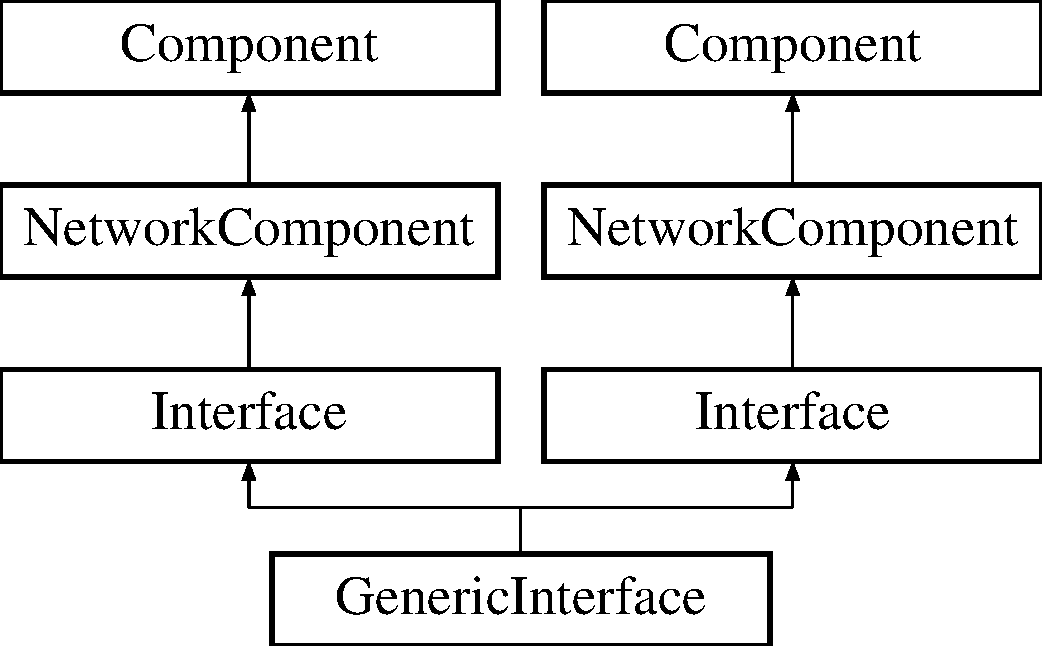
\includegraphics[height=4cm]{classGenericInterface}
\end{center}
\end{figure}
\subsection*{Public Member Functions}
\begin{CompactItemize}
\item 
\hyperlink{classGenericInterface_6614ccfa832a38b9cd2087f28527fa57}{GenericInterface} ()
\item 
\hyperlink{classGenericInterface_8543b504083542c36dc7f11e00895390}{$\sim$GenericInterface} ()
\item 
\hyperlink{outputBuffer_8h_91ad9478d81a7aaf2593e8d9c3d06a14}{uint} \hyperlink{classGenericInterface_82a7ead764982a93e658ce41d198cc69}{get\_\-no\_\-credits} () const 
\item 
void \hyperlink{classGenericInterface_d4d5041bce12cd013a77f476c039c391}{set\_\-no\_\-credits} (int credits)
\item 
void \hyperlink{classGenericInterface_10e019a3cafe243d63587656afc5e79f}{set\_\-no\_\-vcs} (\hyperlink{outputBuffer_8h_91ad9478d81a7aaf2593e8d9c3d06a14}{uint} v)
\item 
void \hyperlink{classGenericInterface_fd1cd1ccd6d355852bee1677cd8b56df}{set\_\-buffer\_\-size} (\hyperlink{outputBuffer_8h_91ad9478d81a7aaf2593e8d9c3d06a14}{uint} b)
\item 
void \hyperlink{classGenericInterface_1aaf2e40e433e913e7ea9cb68693fa7c}{setup} ()
\item 
string \hyperlink{classGenericInterface_ae1400fce0c7ba48965596ec172e474b}{toString} () const 
\item 
void \hyperlink{classGenericInterface_d56b8876204889d3c096fccd61b16b9e}{process\_\-event} (\hyperlink{classIrisEvent}{IrisEvent} $\ast$e)
\item 
string \hyperlink{classGenericInterface_b1be26f08d69932b1ac08094985eb5d6}{print\_\-stats} ()
\item 
\hyperlink{classGenericInterface_6614ccfa832a38b9cd2087f28527fa57}{GenericInterface} ()
\item 
\hyperlink{classGenericInterface_8543b504083542c36dc7f11e00895390}{$\sim$GenericInterface} ()
\item 
\hyperlink{outputBuffer_8h_91ad9478d81a7aaf2593e8d9c3d06a14}{uint} \hyperlink{classGenericInterface_82a7ead764982a93e658ce41d198cc69}{get\_\-no\_\-credits} () const 
\item 
void \hyperlink{classGenericInterface_d4d5041bce12cd013a77f476c039c391}{set\_\-no\_\-credits} (int credits)
\item 
void \hyperlink{classGenericInterface_10e019a3cafe243d63587656afc5e79f}{set\_\-no\_\-vcs} (\hyperlink{outputBuffer_8h_91ad9478d81a7aaf2593e8d9c3d06a14}{uint} v)
\item 
void \hyperlink{classGenericInterface_fd1cd1ccd6d355852bee1677cd8b56df}{set\_\-buffer\_\-size} (\hyperlink{outputBuffer_8h_91ad9478d81a7aaf2593e8d9c3d06a14}{uint} b)
\item 
void \hyperlink{classGenericInterface_1aaf2e40e433e913e7ea9cb68693fa7c}{setup} ()
\item 
string \hyperlink{classGenericInterface_ae1400fce0c7ba48965596ec172e474b}{toString} () const 
\item 
void \hyperlink{classGenericInterface_d56b8876204889d3c096fccd61b16b9e}{process\_\-event} (\hyperlink{classIrisEvent}{IrisEvent} $\ast$e)
\item 
string \hyperlink{classGenericInterface_b1be26f08d69932b1ac08094985eb5d6}{print\_\-stats} ()
\end{CompactItemize}


\subsection{Constructor \& Destructor Documentation}
\hypertarget{classGenericInterface_6614ccfa832a38b9cd2087f28527fa57}{
\index{GenericInterface@{GenericInterface}!GenericInterface@{GenericInterface}}
\index{GenericInterface@{GenericInterface}!GenericInterface@{GenericInterface}}
\subsubsection[{GenericInterface}]{\setlength{\rightskip}{0pt plus 5cm}GenericInterface::GenericInterface ()}}
\label{classGenericInterface_6614ccfa832a38b9cd2087f28527fa57}


\hypertarget{classGenericInterface_8543b504083542c36dc7f11e00895390}{
\index{GenericInterface@{GenericInterface}!$\sim$GenericInterface@{$\sim$GenericInterface}}
\index{$\sim$GenericInterface@{$\sim$GenericInterface}!GenericInterface@{GenericInterface}}
\subsubsection[{$\sim$GenericInterface}]{\setlength{\rightskip}{0pt plus 5cm}GenericInterface::$\sim$GenericInterface ()}}
\label{classGenericInterface_8543b504083542c36dc7f11e00895390}


\hypertarget{classGenericInterface_6614ccfa832a38b9cd2087f28527fa57}{
\index{GenericInterface@{GenericInterface}!GenericInterface@{GenericInterface}}
\index{GenericInterface@{GenericInterface}!GenericInterface@{GenericInterface}}
\subsubsection[{GenericInterface}]{\setlength{\rightskip}{0pt plus 5cm}GenericInterface::GenericInterface ()}}
\label{classGenericInterface_6614ccfa832a38b9cd2087f28527fa57}


\hypertarget{classGenericInterface_8543b504083542c36dc7f11e00895390}{
\index{GenericInterface@{GenericInterface}!$\sim$GenericInterface@{$\sim$GenericInterface}}
\index{$\sim$GenericInterface@{$\sim$GenericInterface}!GenericInterface@{GenericInterface}}
\subsubsection[{$\sim$GenericInterface}]{\setlength{\rightskip}{0pt plus 5cm}GenericInterface::$\sim$GenericInterface ()}}
\label{classGenericInterface_8543b504083542c36dc7f11e00895390}




\subsection{Member Function Documentation}
\hypertarget{classGenericInterface_82a7ead764982a93e658ce41d198cc69}{
\index{GenericInterface@{GenericInterface}!get\_\-no\_\-credits@{get\_\-no\_\-credits}}
\index{get\_\-no\_\-credits@{get\_\-no\_\-credits}!GenericInterface@{GenericInterface}}
\subsubsection[{get\_\-no\_\-credits}]{\setlength{\rightskip}{0pt plus 5cm}{\bf uint} GenericInterface::get\_\-no\_\-credits () const}}
\label{classGenericInterface_82a7ead764982a93e658ce41d198cc69}


\hypertarget{classGenericInterface_82a7ead764982a93e658ce41d198cc69}{
\index{GenericInterface@{GenericInterface}!get\_\-no\_\-credits@{get\_\-no\_\-credits}}
\index{get\_\-no\_\-credits@{get\_\-no\_\-credits}!GenericInterface@{GenericInterface}}
\subsubsection[{get\_\-no\_\-credits}]{\setlength{\rightskip}{0pt plus 5cm}{\bf uint} GenericInterface::get\_\-no\_\-credits () const}}
\label{classGenericInterface_82a7ead764982a93e658ce41d198cc69}


\hypertarget{classGenericInterface_b1be26f08d69932b1ac08094985eb5d6}{
\index{GenericInterface@{GenericInterface}!print\_\-stats@{print\_\-stats}}
\index{print\_\-stats@{print\_\-stats}!GenericInterface@{GenericInterface}}
\subsubsection[{print\_\-stats}]{\setlength{\rightskip}{0pt plus 5cm}string GenericInterface::print\_\-stats ()\hspace{0.3cm}{\tt  \mbox{[}virtual\mbox{]}}}}
\label{classGenericInterface_b1be26f08d69932b1ac08094985eb5d6}




Implements \hyperlink{classInterface_abfe4b675df488fd5a88d2876cff0ebe}{Interface}.\hypertarget{classGenericInterface_b1be26f08d69932b1ac08094985eb5d6}{
\index{GenericInterface@{GenericInterface}!print\_\-stats@{print\_\-stats}}
\index{print\_\-stats@{print\_\-stats}!GenericInterface@{GenericInterface}}
\subsubsection[{print\_\-stats}]{\setlength{\rightskip}{0pt plus 5cm}string GenericInterface::print\_\-stats ()\hspace{0.3cm}{\tt  \mbox{[}virtual\mbox{]}}}}
\label{classGenericInterface_b1be26f08d69932b1ac08094985eb5d6}




Implements \hyperlink{classInterface_abfe4b675df488fd5a88d2876cff0ebe}{Interface}.\hypertarget{classGenericInterface_d56b8876204889d3c096fccd61b16b9e}{
\index{GenericInterface@{GenericInterface}!process\_\-event@{process\_\-event}}
\index{process\_\-event@{process\_\-event}!GenericInterface@{GenericInterface}}
\subsubsection[{process\_\-event}]{\setlength{\rightskip}{0pt plus 5cm}void GenericInterface::process\_\-event ({\bf IrisEvent} $\ast$ {\em e})\hspace{0.3cm}{\tt  \mbox{[}virtual\mbox{]}}}}
\label{classGenericInterface_d56b8876204889d3c096fccd61b16b9e}




Implements \hyperlink{classInterface_baaaeb823b1e0fd7ddc1bb32c2f016fb}{Interface}.\hypertarget{classGenericInterface_d56b8876204889d3c096fccd61b16b9e}{
\index{GenericInterface@{GenericInterface}!process\_\-event@{process\_\-event}}
\index{process\_\-event@{process\_\-event}!GenericInterface@{GenericInterface}}
\subsubsection[{process\_\-event}]{\setlength{\rightskip}{0pt plus 5cm}void GenericInterface::process\_\-event ({\bf IrisEvent} $\ast$ {\em e})\hspace{0.3cm}{\tt  \mbox{[}virtual\mbox{]}}}}
\label{classGenericInterface_d56b8876204889d3c096fccd61b16b9e}




Implements \hyperlink{classInterface_baaaeb823b1e0fd7ddc1bb32c2f016fb}{Interface}.\hypertarget{classGenericInterface_fd1cd1ccd6d355852bee1677cd8b56df}{
\index{GenericInterface@{GenericInterface}!set\_\-buffer\_\-size@{set\_\-buffer\_\-size}}
\index{set\_\-buffer\_\-size@{set\_\-buffer\_\-size}!GenericInterface@{GenericInterface}}
\subsubsection[{set\_\-buffer\_\-size}]{\setlength{\rightskip}{0pt plus 5cm}void GenericInterface::set\_\-buffer\_\-size ({\bf uint} {\em b})\hspace{0.3cm}{\tt  \mbox{[}virtual\mbox{]}}}}
\label{classGenericInterface_fd1cd1ccd6d355852bee1677cd8b56df}




Implements \hyperlink{classInterface_f2cec7f7aa725d52c8bb02087d7c9e5d}{Interface}.\hypertarget{classGenericInterface_fd1cd1ccd6d355852bee1677cd8b56df}{
\index{GenericInterface@{GenericInterface}!set\_\-buffer\_\-size@{set\_\-buffer\_\-size}}
\index{set\_\-buffer\_\-size@{set\_\-buffer\_\-size}!GenericInterface@{GenericInterface}}
\subsubsection[{set\_\-buffer\_\-size}]{\setlength{\rightskip}{0pt plus 5cm}void GenericInterface::set\_\-buffer\_\-size ({\bf uint} {\em b})\hspace{0.3cm}{\tt  \mbox{[}virtual\mbox{]}}}}
\label{classGenericInterface_fd1cd1ccd6d355852bee1677cd8b56df}




Implements \hyperlink{classInterface_f2cec7f7aa725d52c8bb02087d7c9e5d}{Interface}.\hypertarget{classGenericInterface_d4d5041bce12cd013a77f476c039c391}{
\index{GenericInterface@{GenericInterface}!set\_\-no\_\-credits@{set\_\-no\_\-credits}}
\index{set\_\-no\_\-credits@{set\_\-no\_\-credits}!GenericInterface@{GenericInterface}}
\subsubsection[{set\_\-no\_\-credits}]{\setlength{\rightskip}{0pt plus 5cm}void GenericInterface::set\_\-no\_\-credits (int {\em credits})\hspace{0.3cm}{\tt  \mbox{[}virtual\mbox{]}}}}
\label{classGenericInterface_d4d5041bce12cd013a77f476c039c391}




Implements \hyperlink{classInterface_c458ee6d8e974cb0a9f90308d0feb16d}{Interface}.\hypertarget{classGenericInterface_d4d5041bce12cd013a77f476c039c391}{
\index{GenericInterface@{GenericInterface}!set\_\-no\_\-credits@{set\_\-no\_\-credits}}
\index{set\_\-no\_\-credits@{set\_\-no\_\-credits}!GenericInterface@{GenericInterface}}
\subsubsection[{set\_\-no\_\-credits}]{\setlength{\rightskip}{0pt plus 5cm}void GenericInterface::set\_\-no\_\-credits (int {\em credits})\hspace{0.3cm}{\tt  \mbox{[}virtual\mbox{]}}}}
\label{classGenericInterface_d4d5041bce12cd013a77f476c039c391}




Implements \hyperlink{classInterface_c458ee6d8e974cb0a9f90308d0feb16d}{Interface}.\hypertarget{classGenericInterface_10e019a3cafe243d63587656afc5e79f}{
\index{GenericInterface@{GenericInterface}!set\_\-no\_\-vcs@{set\_\-no\_\-vcs}}
\index{set\_\-no\_\-vcs@{set\_\-no\_\-vcs}!GenericInterface@{GenericInterface}}
\subsubsection[{set\_\-no\_\-vcs}]{\setlength{\rightskip}{0pt plus 5cm}void GenericInterface::set\_\-no\_\-vcs ({\bf uint} {\em v})\hspace{0.3cm}{\tt  \mbox{[}virtual\mbox{]}}}}
\label{classGenericInterface_10e019a3cafe243d63587656afc5e79f}




Implements \hyperlink{classInterface_e7266de6cc9e1dfd4bb3a1b8face3c15}{Interface}.\hypertarget{classGenericInterface_10e019a3cafe243d63587656afc5e79f}{
\index{GenericInterface@{GenericInterface}!set\_\-no\_\-vcs@{set\_\-no\_\-vcs}}
\index{set\_\-no\_\-vcs@{set\_\-no\_\-vcs}!GenericInterface@{GenericInterface}}
\subsubsection[{set\_\-no\_\-vcs}]{\setlength{\rightskip}{0pt plus 5cm}void GenericInterface::set\_\-no\_\-vcs ({\bf uint} {\em v})\hspace{0.3cm}{\tt  \mbox{[}virtual\mbox{]}}}}
\label{classGenericInterface_10e019a3cafe243d63587656afc5e79f}




Implements \hyperlink{classInterface_e7266de6cc9e1dfd4bb3a1b8face3c15}{Interface}.\hypertarget{classGenericInterface_1aaf2e40e433e913e7ea9cb68693fa7c}{
\index{GenericInterface@{GenericInterface}!setup@{setup}}
\index{setup@{setup}!GenericInterface@{GenericInterface}}
\subsubsection[{setup}]{\setlength{\rightskip}{0pt plus 5cm}void GenericInterface::setup ()\hspace{0.3cm}{\tt  \mbox{[}virtual\mbox{]}}}}
\label{classGenericInterface_1aaf2e40e433e913e7ea9cb68693fa7c}




Implements \hyperlink{classInterface_f9015204e6dabe3e0fce572b19cd1550}{Interface}.\hypertarget{classGenericInterface_1aaf2e40e433e913e7ea9cb68693fa7c}{
\index{GenericInterface@{GenericInterface}!setup@{setup}}
\index{setup@{setup}!GenericInterface@{GenericInterface}}
\subsubsection[{setup}]{\setlength{\rightskip}{0pt plus 5cm}void GenericInterface::setup ()\hspace{0.3cm}{\tt  \mbox{[}virtual\mbox{]}}}}
\label{classGenericInterface_1aaf2e40e433e913e7ea9cb68693fa7c}




Implements \hyperlink{classInterface_f9015204e6dabe3e0fce572b19cd1550}{Interface}.\hypertarget{classGenericInterface_ae1400fce0c7ba48965596ec172e474b}{
\index{GenericInterface@{GenericInterface}!toString@{toString}}
\index{toString@{toString}!GenericInterface@{GenericInterface}}
\subsubsection[{toString}]{\setlength{\rightskip}{0pt plus 5cm}string GenericInterface::toString () const\hspace{0.3cm}{\tt  \mbox{[}virtual\mbox{]}}}}
\label{classGenericInterface_ae1400fce0c7ba48965596ec172e474b}




Reimplemented from \hyperlink{classInterface_137cdb3bca46eb2ae0bbf017d1efb66e}{Interface}.\hypertarget{classGenericInterface_ae1400fce0c7ba48965596ec172e474b}{
\index{GenericInterface@{GenericInterface}!toString@{toString}}
\index{toString@{toString}!GenericInterface@{GenericInterface}}
\subsubsection[{toString}]{\setlength{\rightskip}{0pt plus 5cm}string GenericInterface::toString () const\hspace{0.3cm}{\tt  \mbox{[}virtual\mbox{]}}}}
\label{classGenericInterface_ae1400fce0c7ba48965596ec172e474b}




Reimplemented from \hyperlink{classInterface_137cdb3bca46eb2ae0bbf017d1efb66e}{Interface}.

The documentation for this class was generated from the following files:\begin{CompactItemize}
\item 
source/components/impl/\hyperlink{impl_2genericInterface_8h}{genericInterface.h}\item 
source/components/none/\hyperlink{none_2genericInterface_8h}{genericInterface.h}\item 
source/components/impl/\hyperlink{impl_2genericInterface_8cc}{genericInterface.cc}\item 
source/components/none/\hyperlink{none_2genericInterface_8cc}{genericInterface.cc}\end{CompactItemize}

\hypertarget{classGenericLink}{
\section{GenericLink Class Reference}
\label{classGenericLink}\index{GenericLink@{GenericLink}}
}
{\tt \#include $<$genericLink.h$>$}

Inheritance diagram for GenericLink::\begin{figure}[H]
\begin{center}
\leavevmode
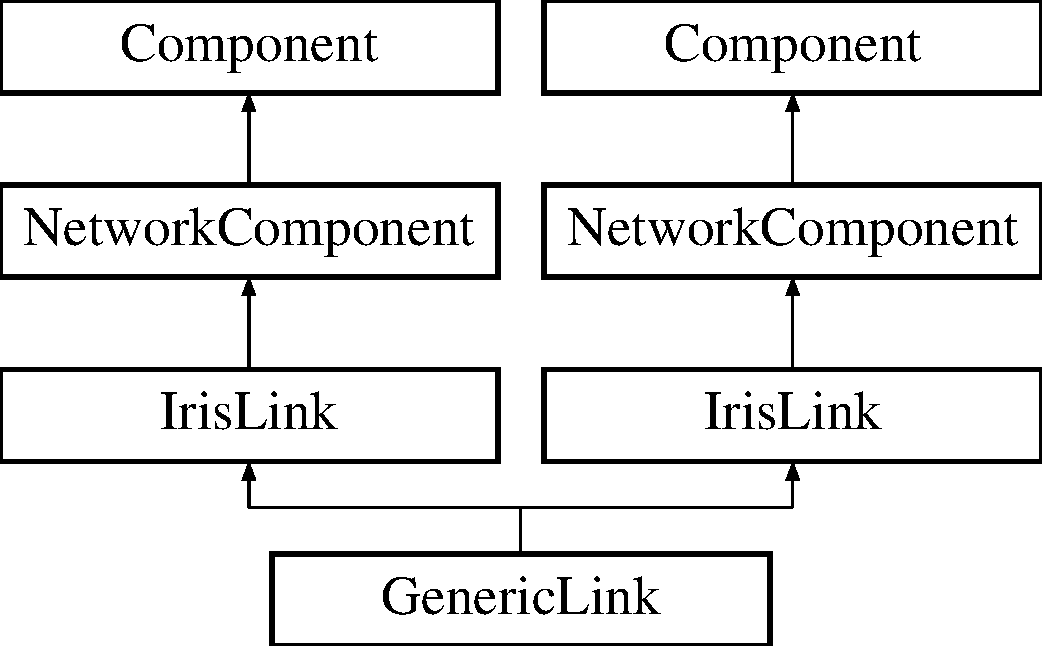
\includegraphics[height=4cm]{classGenericLink}
\end{center}
\end{figure}
\subsection*{Public Member Functions}
\begin{CompactItemize}
\item 
\hyperlink{classGenericLink_228314904a07730170bfe994177f33b4}{GenericLink} ()
\item 
\hyperlink{classGenericLink_c67cbdcd115d4e41db4c379119bfdcc4}{$\sim$GenericLink} ()
\item 
void \hyperlink{classGenericLink_8afec492b9c0a403462c2cf1001adc77}{setup} ()
\item 
void \hyperlink{classGenericLink_c09533f8445eb3c550c744fd4ada7324}{process\_\-event} (\hyperlink{classIrisEvent}{IrisEvent} $\ast$e)
\item 
string \hyperlink{classGenericLink_64dad2c98848fb48b3b572887031167b}{toString} () const 
\item 
string \hyperlink{classGenericLink_10ccb365b945b9ad7ea3b49c68069d41}{print\_\-stats} () const 
\item 
\hyperlink{classGenericLink_228314904a07730170bfe994177f33b4}{GenericLink} ()
\item 
\hyperlink{classGenericLink_c67cbdcd115d4e41db4c379119bfdcc4}{$\sim$GenericLink} ()
\item 
void \hyperlink{classGenericLink_8afec492b9c0a403462c2cf1001adc77}{setup} ()
\item 
void \hyperlink{classGenericLink_c09533f8445eb3c550c744fd4ada7324}{process\_\-event} (\hyperlink{classIrisEvent}{IrisEvent} $\ast$e)
\item 
string \hyperlink{classGenericLink_64dad2c98848fb48b3b572887031167b}{toString} () const 
\item 
string \hyperlink{classGenericLink_10ccb365b945b9ad7ea3b49c68069d41}{print\_\-stats} () const 
\end{CompactItemize}
\subsection*{Public Attributes}
\begin{CompactItemize}
\item 
\hyperlink{outputBuffer_8h_91ad9478d81a7aaf2593e8d9c3d06a14}{uint} \hyperlink{classGenericLink_b4188829f4bf0096117b2d81517f1201}{cycles}
\item 
\hyperlink{outputBuffer_8h_91ad9478d81a7aaf2593e8d9c3d06a14}{uint} \hyperlink{classGenericLink_7c2197f0b770d473c2ee0305967bfad7}{stages}
\end{CompactItemize}


\subsection{Constructor \& Destructor Documentation}
\hypertarget{classGenericLink_228314904a07730170bfe994177f33b4}{
\index{GenericLink@{GenericLink}!GenericLink@{GenericLink}}
\index{GenericLink@{GenericLink}!GenericLink@{GenericLink}}
\subsubsection[{GenericLink}]{\setlength{\rightskip}{0pt plus 5cm}GenericLink::GenericLink ()\hspace{0.3cm}{\tt  \mbox{[}inline\mbox{]}}}}
\label{classGenericLink_228314904a07730170bfe994177f33b4}


\hypertarget{classGenericLink_c67cbdcd115d4e41db4c379119bfdcc4}{
\index{GenericLink@{GenericLink}!$\sim$GenericLink@{$\sim$GenericLink}}
\index{$\sim$GenericLink@{$\sim$GenericLink}!GenericLink@{GenericLink}}
\subsubsection[{$\sim$GenericLink}]{\setlength{\rightskip}{0pt plus 5cm}GenericLink::$\sim$GenericLink ()\hspace{0.3cm}{\tt  \mbox{[}inline\mbox{]}}}}
\label{classGenericLink_c67cbdcd115d4e41db4c379119bfdcc4}


\hypertarget{classGenericLink_228314904a07730170bfe994177f33b4}{
\index{GenericLink@{GenericLink}!GenericLink@{GenericLink}}
\index{GenericLink@{GenericLink}!GenericLink@{GenericLink}}
\subsubsection[{GenericLink}]{\setlength{\rightskip}{0pt plus 5cm}GenericLink::GenericLink ()\hspace{0.3cm}{\tt  \mbox{[}inline\mbox{]}}}}
\label{classGenericLink_228314904a07730170bfe994177f33b4}


\hypertarget{classGenericLink_c67cbdcd115d4e41db4c379119bfdcc4}{
\index{GenericLink@{GenericLink}!$\sim$GenericLink@{$\sim$GenericLink}}
\index{$\sim$GenericLink@{$\sim$GenericLink}!GenericLink@{GenericLink}}
\subsubsection[{$\sim$GenericLink}]{\setlength{\rightskip}{0pt plus 5cm}GenericLink::$\sim$GenericLink ()\hspace{0.3cm}{\tt  \mbox{[}inline\mbox{]}}}}
\label{classGenericLink_c67cbdcd115d4e41db4c379119bfdcc4}




\subsection{Member Function Documentation}
\hypertarget{classGenericLink_10ccb365b945b9ad7ea3b49c68069d41}{
\index{GenericLink@{GenericLink}!print\_\-stats@{print\_\-stats}}
\index{print\_\-stats@{print\_\-stats}!GenericLink@{GenericLink}}
\subsubsection[{print\_\-stats}]{\setlength{\rightskip}{0pt plus 5cm}string GenericLink::print\_\-stats () const}}
\label{classGenericLink_10ccb365b945b9ad7ea3b49c68069d41}


\hypertarget{classGenericLink_10ccb365b945b9ad7ea3b49c68069d41}{
\index{GenericLink@{GenericLink}!print\_\-stats@{print\_\-stats}}
\index{print\_\-stats@{print\_\-stats}!GenericLink@{GenericLink}}
\subsubsection[{print\_\-stats}]{\setlength{\rightskip}{0pt plus 5cm}string GenericLink::print\_\-stats () const}}
\label{classGenericLink_10ccb365b945b9ad7ea3b49c68069d41}


\hypertarget{classGenericLink_c09533f8445eb3c550c744fd4ada7324}{
\index{GenericLink@{GenericLink}!process\_\-event@{process\_\-event}}
\index{process\_\-event@{process\_\-event}!GenericLink@{GenericLink}}
\subsubsection[{process\_\-event}]{\setlength{\rightskip}{0pt plus 5cm}void GenericLink::process\_\-event ({\bf IrisEvent} $\ast$ {\em e})\hspace{0.3cm}{\tt  \mbox{[}virtual\mbox{]}}}}
\label{classGenericLink_c09533f8445eb3c550c744fd4ada7324}




Implements \hyperlink{classIrisLink_9c5494bc5716aedf3affe748f3a542c1}{IrisLink}.\hypertarget{classGenericLink_c09533f8445eb3c550c744fd4ada7324}{
\index{GenericLink@{GenericLink}!process\_\-event@{process\_\-event}}
\index{process\_\-event@{process\_\-event}!GenericLink@{GenericLink}}
\subsubsection[{process\_\-event}]{\setlength{\rightskip}{0pt plus 5cm}void GenericLink::process\_\-event ({\bf IrisEvent} $\ast$ {\em e})\hspace{0.3cm}{\tt  \mbox{[}virtual\mbox{]}}}}
\label{classGenericLink_c09533f8445eb3c550c744fd4ada7324}




Implements \hyperlink{classIrisLink_9c5494bc5716aedf3affe748f3a542c1}{IrisLink}.\hypertarget{classGenericLink_8afec492b9c0a403462c2cf1001adc77}{
\index{GenericLink@{GenericLink}!setup@{setup}}
\index{setup@{setup}!GenericLink@{GenericLink}}
\subsubsection[{setup}]{\setlength{\rightskip}{0pt plus 5cm}void GenericLink::setup ()}}
\label{classGenericLink_8afec492b9c0a403462c2cf1001adc77}


\hypertarget{classGenericLink_8afec492b9c0a403462c2cf1001adc77}{
\index{GenericLink@{GenericLink}!setup@{setup}}
\index{setup@{setup}!GenericLink@{GenericLink}}
\subsubsection[{setup}]{\setlength{\rightskip}{0pt plus 5cm}void GenericLink::setup ()}}
\label{classGenericLink_8afec492b9c0a403462c2cf1001adc77}


\hypertarget{classGenericLink_64dad2c98848fb48b3b572887031167b}{
\index{GenericLink@{GenericLink}!toString@{toString}}
\index{toString@{toString}!GenericLink@{GenericLink}}
\subsubsection[{toString}]{\setlength{\rightskip}{0pt plus 5cm}string GenericLink::toString () const\hspace{0.3cm}{\tt  \mbox{[}virtual\mbox{]}}}}
\label{classGenericLink_64dad2c98848fb48b3b572887031167b}




Reimplemented from \hyperlink{classIrisLink_d25db1c98385d7abd82180e5746813a6}{IrisLink}.\hypertarget{classGenericLink_64dad2c98848fb48b3b572887031167b}{
\index{GenericLink@{GenericLink}!toString@{toString}}
\index{toString@{toString}!GenericLink@{GenericLink}}
\subsubsection[{toString}]{\setlength{\rightskip}{0pt plus 5cm}string GenericLink::toString () const\hspace{0.3cm}{\tt  \mbox{[}virtual\mbox{]}}}}
\label{classGenericLink_64dad2c98848fb48b3b572887031167b}




Reimplemented from \hyperlink{classIrisLink_d25db1c98385d7abd82180e5746813a6}{IrisLink}.

\subsection{Member Data Documentation}
\hypertarget{classGenericLink_b4188829f4bf0096117b2d81517f1201}{
\index{GenericLink@{GenericLink}!cycles@{cycles}}
\index{cycles@{cycles}!GenericLink@{GenericLink}}
\subsubsection[{cycles}]{\setlength{\rightskip}{0pt plus 5cm}{\bf uint} {\bf GenericLink::cycles}}}
\label{classGenericLink_b4188829f4bf0096117b2d81517f1201}


\hypertarget{classGenericLink_7c2197f0b770d473c2ee0305967bfad7}{
\index{GenericLink@{GenericLink}!stages@{stages}}
\index{stages@{stages}!GenericLink@{GenericLink}}
\subsubsection[{stages}]{\setlength{\rightskip}{0pt plus 5cm}{\bf uint} {\bf GenericLink::stages}}}
\label{classGenericLink_7c2197f0b770d473c2ee0305967bfad7}




The documentation for this class was generated from the following files:\begin{CompactItemize}
\item 
source/components/impl/\hyperlink{impl_2genericLink_8h}{genericLink.h}\item 
source/components/none/\hyperlink{none_2genericLink_8h}{genericLink.h}\item 
source/components/impl/\hyperlink{impl_2genericLink_8cc}{genericLink.cc}\item 
source/components/none/\hyperlink{none_2genericLink_8cc}{genericLink.cc}\end{CompactItemize}

\hypertarget{classGenericNetworkSource}{
\section{GenericNetworkSource Class Reference}
\label{classGenericNetworkSource}\index{GenericNetworkSource@{GenericNetworkSource}}
}
{\tt \#include $<$networkSource.h$>$}

Inheritance diagram for GenericNetworkSource::\begin{figure}[H]
\begin{center}
\leavevmode
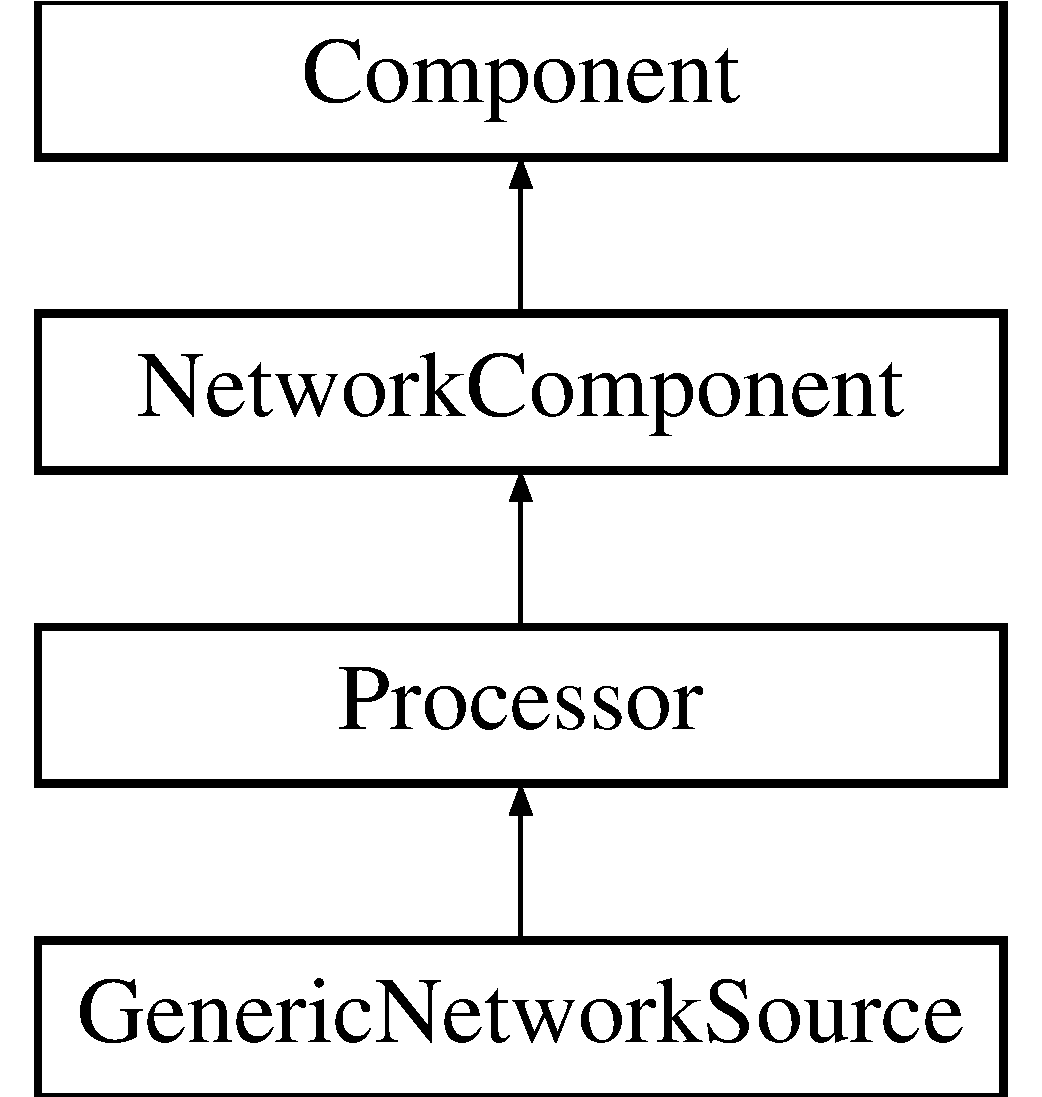
\includegraphics[height=4cm]{classGenericNetworkSource}
\end{center}
\end{figure}
\subsection*{Public Member Functions}
\begin{CompactItemize}
\item 
\hyperlink{classGenericNetworkSource_66fa04f8ab4c8ac70192f63249f8b387}{GenericNetworkSource} ()
\item 
virtual \hyperlink{classGenericNetworkSource_de83e8c46d7c400be8bdd2cf1e33d765}{$\sim$GenericNetworkSource} ()
\item 
unsigned long int \hyperlink{classGenericNetworkSource_a1970b5e7d100e15d282f03358c8ce70}{max\_\-time} ()
\item 
void \hyperlink{classGenericNetworkSource_a1390d4685120020d9b9564ee19df854}{setup} ()
\item 
void \hyperlink{classGenericNetworkSource_e875a5cd3f60bd3073812f747c80409e}{init} ()
\item 
void \hyperlink{classGenericNetworkSource_a67be5ac0f97b7e0b38eba909cecaa64}{process\_\-event} (\hyperlink{classIrisEvent}{IrisEvent} $\ast$e)
\item 
string \hyperlink{classGenericNetworkSource_8d8c0760eb634da3ccc3d4083e9415b9}{toString} () const 
\end{CompactItemize}
\subsection*{Public Attributes}
\begin{CompactItemize}
\item 
\hyperlink{classNetworkComponent}{NetworkComponent} $\ast$ \hyperlink{classGenericNetworkSource_394c482da644893d93513f202850cec0}{output\_\-connection}
\item 
\hyperlink{classNetworkComponent}{NetworkComponent} $\ast$ \hyperlink{classGenericNetworkSource_49ae0bba9107dfecd501b5ba5ff9ddc1}{input\_\-connection}
\item 
\hyperlink{outputBuffer_8h_91ad9478d81a7aaf2593e8d9c3d06a14}{uint} \hyperlink{classGenericNetworkSource_90d400349086508bb6b2b46fbd24ed9b}{node\_\-ip}
\item 
\hyperlink{classGenericOutputBuffer}{GenericOutputBuffer} \hyperlink{classGenericNetworkSource_5d6de27fc38a82fa7efd029ab79e4ab6}{out\_\-buffer}
\end{CompactItemize}


\subsection{Constructor \& Destructor Documentation}
\hypertarget{classGenericNetworkSource_66fa04f8ab4c8ac70192f63249f8b387}{
\index{GenericNetworkSource@{GenericNetworkSource}!GenericNetworkSource@{GenericNetworkSource}}
\index{GenericNetworkSource@{GenericNetworkSource}!GenericNetworkSource@{GenericNetworkSource}}
\subsubsection[{GenericNetworkSource}]{\setlength{\rightskip}{0pt plus 5cm}GenericNetworkSource::GenericNetworkSource ()}}
\label{classGenericNetworkSource_66fa04f8ab4c8ac70192f63249f8b387}


\hypertarget{classGenericNetworkSource_de83e8c46d7c400be8bdd2cf1e33d765}{
\index{GenericNetworkSource@{GenericNetworkSource}!$\sim$GenericNetworkSource@{$\sim$GenericNetworkSource}}
\index{$\sim$GenericNetworkSource@{$\sim$GenericNetworkSource}!GenericNetworkSource@{GenericNetworkSource}}
\subsubsection[{$\sim$GenericNetworkSource}]{\setlength{\rightskip}{0pt plus 5cm}virtual GenericNetworkSource::$\sim$GenericNetworkSource ()\hspace{0.3cm}{\tt  \mbox{[}inline, virtual\mbox{]}}}}
\label{classGenericNetworkSource_de83e8c46d7c400be8bdd2cf1e33d765}




\subsection{Member Function Documentation}
\hypertarget{classGenericNetworkSource_e875a5cd3f60bd3073812f747c80409e}{
\index{GenericNetworkSource@{GenericNetworkSource}!init@{init}}
\index{init@{init}!GenericNetworkSource@{GenericNetworkSource}}
\subsubsection[{init}]{\setlength{\rightskip}{0pt plus 5cm}void GenericNetworkSource::init ()}}
\label{classGenericNetworkSource_e875a5cd3f60bd3073812f747c80409e}




Reimplemented from \hyperlink{classProcessor_22e869ee49d974ad0ee7ee81961ab88f}{Processor}.\hypertarget{classGenericNetworkSource_a1970b5e7d100e15d282f03358c8ce70}{
\index{GenericNetworkSource@{GenericNetworkSource}!max\_\-time@{max\_\-time}}
\index{max\_\-time@{max\_\-time}!GenericNetworkSource@{GenericNetworkSource}}
\subsubsection[{max\_\-time}]{\setlength{\rightskip}{0pt plus 5cm}unsigned long int GenericNetworkSource::max\_\-time ()}}
\label{classGenericNetworkSource_a1970b5e7d100e15d282f03358c8ce70}


\hypertarget{classGenericNetworkSource_a67be5ac0f97b7e0b38eba909cecaa64}{
\index{GenericNetworkSource@{GenericNetworkSource}!process\_\-event@{process\_\-event}}
\index{process\_\-event@{process\_\-event}!GenericNetworkSource@{GenericNetworkSource}}
\subsubsection[{process\_\-event}]{\setlength{\rightskip}{0pt plus 5cm}void GenericNetworkSource::process\_\-event ({\bf IrisEvent} $\ast$ {\em e})\hspace{0.3cm}{\tt  \mbox{[}virtual\mbox{]}}}}
\label{classGenericNetworkSource_a67be5ac0f97b7e0b38eba909cecaa64}




Implements \hyperlink{classProcessor_18cdeefafbd8225cb3ad18dd098c0e08}{Processor}.\hypertarget{classGenericNetworkSource_a1390d4685120020d9b9564ee19df854}{
\index{GenericNetworkSource@{GenericNetworkSource}!setup@{setup}}
\index{setup@{setup}!GenericNetworkSource@{GenericNetworkSource}}
\subsubsection[{setup}]{\setlength{\rightskip}{0pt plus 5cm}void GenericNetworkSource::setup ()\hspace{0.3cm}{\tt  \mbox{[}virtual\mbox{]}}}}
\label{classGenericNetworkSource_a1390d4685120020d9b9564ee19df854}




Implements \hyperlink{classProcessor_495fad01358e2d9760c526d6e2db53ea}{Processor}.\hypertarget{classGenericNetworkSource_8d8c0760eb634da3ccc3d4083e9415b9}{
\index{GenericNetworkSource@{GenericNetworkSource}!toString@{toString}}
\index{toString@{toString}!GenericNetworkSource@{GenericNetworkSource}}
\subsubsection[{toString}]{\setlength{\rightskip}{0pt plus 5cm}string GenericNetworkSource::toString (void) const\hspace{0.3cm}{\tt  \mbox{[}virtual\mbox{]}}}}
\label{classGenericNetworkSource_8d8c0760eb634da3ccc3d4083e9415b9}




Reimplemented from \hyperlink{classProcessor_d3bdbedfbb00b05f61504e411a418106}{Processor}.

\subsection{Member Data Documentation}
\hypertarget{classGenericNetworkSource_49ae0bba9107dfecd501b5ba5ff9ddc1}{
\index{GenericNetworkSource@{GenericNetworkSource}!input\_\-connection@{input\_\-connection}}
\index{input\_\-connection@{input\_\-connection}!GenericNetworkSource@{GenericNetworkSource}}
\subsubsection[{input\_\-connection}]{\setlength{\rightskip}{0pt plus 5cm}{\bf NetworkComponent}$\ast$ {\bf GenericNetworkSource::input\_\-connection}}}
\label{classGenericNetworkSource_49ae0bba9107dfecd501b5ba5ff9ddc1}


\hypertarget{classGenericNetworkSource_90d400349086508bb6b2b46fbd24ed9b}{
\index{GenericNetworkSource@{GenericNetworkSource}!node\_\-ip@{node\_\-ip}}
\index{node\_\-ip@{node\_\-ip}!GenericNetworkSource@{GenericNetworkSource}}
\subsubsection[{node\_\-ip}]{\setlength{\rightskip}{0pt plus 5cm}{\bf uint} {\bf GenericNetworkSource::node\_\-ip}}}
\label{classGenericNetworkSource_90d400349086508bb6b2b46fbd24ed9b}




Reimplemented from \hyperlink{classNetworkComponent_56599b3484333fb78af1b6c33f77cf16}{NetworkComponent}.\hypertarget{classGenericNetworkSource_5d6de27fc38a82fa7efd029ab79e4ab6}{
\index{GenericNetworkSource@{GenericNetworkSource}!out\_\-buffer@{out\_\-buffer}}
\index{out\_\-buffer@{out\_\-buffer}!GenericNetworkSource@{GenericNetworkSource}}
\subsubsection[{out\_\-buffer}]{\setlength{\rightskip}{0pt plus 5cm}{\bf GenericOutputBuffer} {\bf GenericNetworkSource::out\_\-buffer}}}
\label{classGenericNetworkSource_5d6de27fc38a82fa7efd029ab79e4ab6}


\hypertarget{classGenericNetworkSource_394c482da644893d93513f202850cec0}{
\index{GenericNetworkSource@{GenericNetworkSource}!output\_\-connection@{output\_\-connection}}
\index{output\_\-connection@{output\_\-connection}!GenericNetworkSource@{GenericNetworkSource}}
\subsubsection[{output\_\-connection}]{\setlength{\rightskip}{0pt plus 5cm}{\bf NetworkComponent}$\ast$ {\bf GenericNetworkSource::output\_\-connection}}}
\label{classGenericNetworkSource_394c482da644893d93513f202850cec0}




The documentation for this class was generated from the following files:\begin{CompactItemize}
\item 
source/tests/\hyperlink{networkSource_8h}{networkSource.h}\item 
source/tests/\hyperlink{networkSink_8cc}{networkSink.cc}\item 
source/tests/\hyperlink{networkSource_8cc}{networkSource.cc}\end{CompactItemize}

\hypertarget{classGenericOutputBuffer}{
\section{GenericOutputBuffer Class Reference}
\label{classGenericOutputBuffer}\index{GenericOutputBuffer@{GenericOutputBuffer}}
}
{\tt \#include $<$genericBuffer.h$>$}

Inheritance diagram for GenericOutputBuffer::\begin{figure}[H]
\begin{center}
\leavevmode
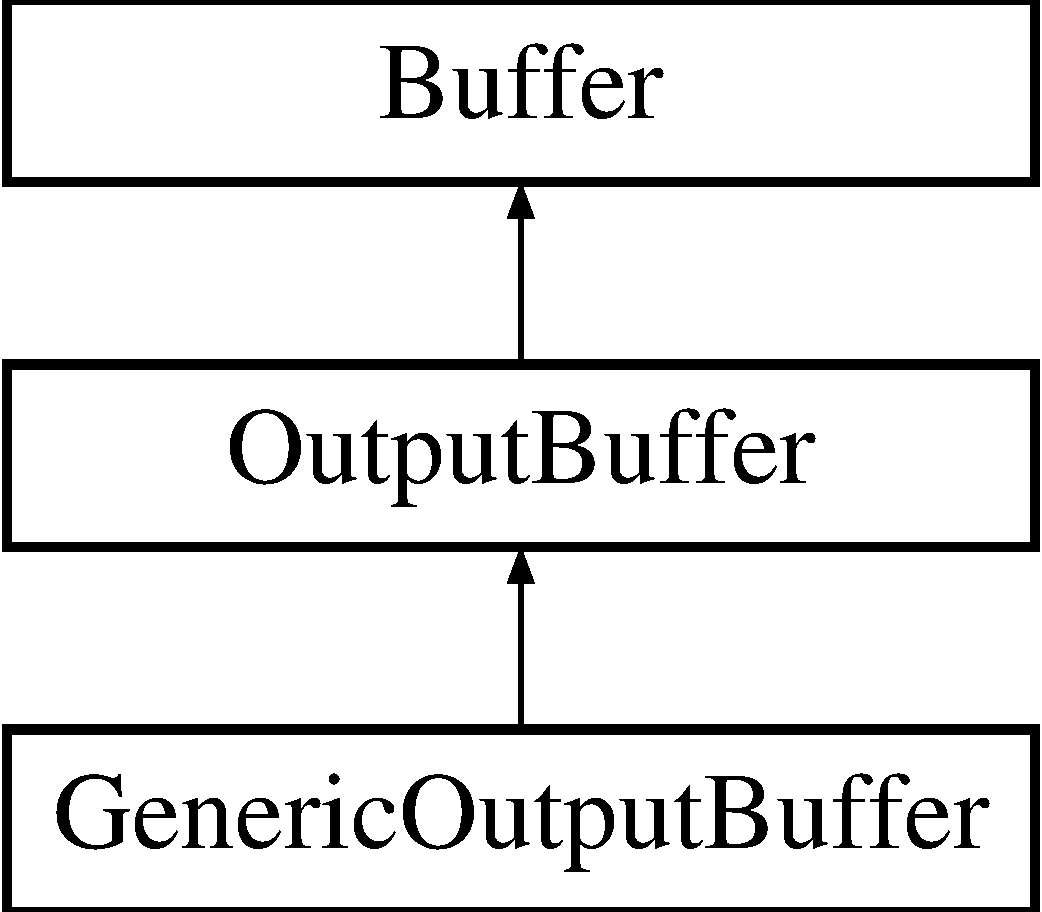
\includegraphics[height=3cm]{classGenericOutputBuffer}
\end{center}
\end{figure}
\subsection*{Public Member Functions}
\begin{CompactItemize}
\item 
\hyperlink{classGenericOutputBuffer_10c4287e27f634982bc28e1de2b31757}{GenericOutputBuffer} ()
\item 
\hyperlink{classGenericOutputBuffer_d67316556a00a71d7b98818de74328ff}{$\sim$GenericOutputBuffer} ()
\item 
void \hyperlink{classGenericOutputBuffer_f2b4047e054df5bb9b624ce0b0bbf0e2}{push} (\hyperlink{classFlit}{Flit} $\ast$f)
\item 
\hyperlink{classFlit}{Flit} $\ast$ \hyperlink{classGenericOutputBuffer_3c3f1b425635f59b0539805945ddb1bd}{pull} ()
\item 
\hyperlink{outputBuffer_8h_91ad9478d81a7aaf2593e8d9c3d06a14}{uint} \hyperlink{classGenericOutputBuffer_0b8b70b9b3ab71195eea8d0d810dce94}{get\_\-occupancy} (\hyperlink{outputBuffer_8h_91ad9478d81a7aaf2593e8d9c3d06a14}{uint} ch) const 
\item 
void \hyperlink{classGenericOutputBuffer_a0dcb541c9d64d097a21dd8b290c3950}{set\_\-no\_\-vcs} (\hyperlink{outputBuffer_8h_91ad9478d81a7aaf2593e8d9c3d06a14}{uint} vcs)
\item 
\hyperlink{outputBuffer_8h_91ad9478d81a7aaf2593e8d9c3d06a14}{uint} \hyperlink{classGenericOutputBuffer_6f5495e1ddd1b524d105d86b083e85cc}{get\_\-no\_\-vcs} () const 
\item 
void \hyperlink{classGenericOutputBuffer_c4f3cf09d07b340af349820bcaed731e}{change\_\-pull\_\-channel} (\hyperlink{outputBuffer_8h_91ad9478d81a7aaf2593e8d9c3d06a14}{uint} ch)
\item 
void \hyperlink{classGenericOutputBuffer_d7576df13afbc101eb997e35ad417739}{change\_\-push\_\-channel} (\hyperlink{outputBuffer_8h_91ad9478d81a7aaf2593e8d9c3d06a14}{uint} ch)
\item 
\hyperlink{outputBuffer_8h_91ad9478d81a7aaf2593e8d9c3d06a14}{uint} \hyperlink{classGenericOutputBuffer_c3e3831a4eb7b09b053b511722e89daf}{get\_\-pull\_\-channel} () const 
\item 
\hyperlink{outputBuffer_8h_91ad9478d81a7aaf2593e8d9c3d06a14}{uint} \hyperlink{classGenericOutputBuffer_d7f10031a96719bc97a11d3a96f4ef6f}{get\_\-push\_\-channel} () const 
\item 
bool \hyperlink{classGenericOutputBuffer_cc3ce27817dea583b8c0cb269b3c9cdb}{is\_\-channel\_\-full} (\hyperlink{outputBuffer_8h_91ad9478d81a7aaf2593e8d9c3d06a14}{uint} ch) const 
\item 
bool \hyperlink{classGenericOutputBuffer_df867815a21d8e832ba19aa63fa65e55}{is\_\-empty} (\hyperlink{outputBuffer_8h_91ad9478d81a7aaf2593e8d9c3d06a14}{uint} ch) const 
\item 
string \hyperlink{classGenericOutputBuffer_746612d97dbd6240764632638931d3fa}{toString} () const 
\item 
void \hyperlink{classGenericOutputBuffer_a61d09c8b3fcdd15b71f1b01d28ea748}{got\_\-credit} (\hyperlink{outputBuffer_8h_91ad9478d81a7aaf2593e8d9c3d06a14}{uint} ch)
\item 
\hyperlink{outputBuffer_8h_91ad9478d81a7aaf2593e8d9c3d06a14}{uint} \hyperlink{classGenericOutputBuffer_20a0a495d2b0aa4e6c6539209038ab2c}{get\_\-no\_\-credits} (\hyperlink{outputBuffer_8h_91ad9478d81a7aaf2593e8d9c3d06a14}{uint} ch) const 
\item 
void \hyperlink{classGenericOutputBuffer_632ffda3db2c9729e2d9d6d1645defb3}{set\_\-no\_\-credits} (\hyperlink{outputBuffer_8h_91ad9478d81a7aaf2593e8d9c3d06a14}{uint} no)
\end{CompactItemize}
\subsection*{Public Attributes}
\begin{CompactItemize}
\item 
\hyperlink{outputBuffer_8h_91ad9478d81a7aaf2593e8d9c3d06a14}{uint} \hyperlink{classGenericOutputBuffer_98d12e7f17f1ce56b89db973b9efe7b0}{buffer\_\-size}
\item 
unsigned long long int \hyperlink{classGenericOutputBuffer_f201a673a51bd864907116c48a053f97}{write\_\-time}
\item 
vector$<$ queue$<$ \hyperlink{classFlit}{Flit} $\ast$ $>$ $>$ \hyperlink{classGenericOutputBuffer_561cd725dc95f8c57fda666df9980313}{buffers}
\item 
vector$<$ int $>$ \hyperlink{classGenericOutputBuffer_fadacb202322788766670e54b1d8430c}{next\_\-port}
\end{CompactItemize}


\subsection{Constructor \& Destructor Documentation}
\hypertarget{classGenericOutputBuffer_10c4287e27f634982bc28e1de2b31757}{
\index{GenericOutputBuffer@{GenericOutputBuffer}!GenericOutputBuffer@{GenericOutputBuffer}}
\index{GenericOutputBuffer@{GenericOutputBuffer}!GenericOutputBuffer@{GenericOutputBuffer}}
\subsubsection[{GenericOutputBuffer}]{\setlength{\rightskip}{0pt plus 5cm}GenericOutputBuffer::GenericOutputBuffer ()}}
\label{classGenericOutputBuffer_10c4287e27f634982bc28e1de2b31757}


\hypertarget{classGenericOutputBuffer_d67316556a00a71d7b98818de74328ff}{
\index{GenericOutputBuffer@{GenericOutputBuffer}!$\sim$GenericOutputBuffer@{$\sim$GenericOutputBuffer}}
\index{$\sim$GenericOutputBuffer@{$\sim$GenericOutputBuffer}!GenericOutputBuffer@{GenericOutputBuffer}}
\subsubsection[{$\sim$GenericOutputBuffer}]{\setlength{\rightskip}{0pt plus 5cm}GenericOutputBuffer::$\sim$GenericOutputBuffer ()}}
\label{classGenericOutputBuffer_d67316556a00a71d7b98818de74328ff}




\subsection{Member Function Documentation}
\hypertarget{classGenericOutputBuffer_c4f3cf09d07b340af349820bcaed731e}{
\index{GenericOutputBuffer@{GenericOutputBuffer}!change\_\-pull\_\-channel@{change\_\-pull\_\-channel}}
\index{change\_\-pull\_\-channel@{change\_\-pull\_\-channel}!GenericOutputBuffer@{GenericOutputBuffer}}
\subsubsection[{change\_\-pull\_\-channel}]{\setlength{\rightskip}{0pt plus 5cm}void GenericOutputBuffer::change\_\-pull\_\-channel ({\bf uint} {\em ch})\hspace{0.3cm}{\tt  \mbox{[}virtual\mbox{]}}}}
\label{classGenericOutputBuffer_c4f3cf09d07b340af349820bcaed731e}




Implements \hyperlink{classOutputBuffer_fb8e0a16f34dcff4c0d954201712f762}{OutputBuffer}.\hypertarget{classGenericOutputBuffer_d7576df13afbc101eb997e35ad417739}{
\index{GenericOutputBuffer@{GenericOutputBuffer}!change\_\-push\_\-channel@{change\_\-push\_\-channel}}
\index{change\_\-push\_\-channel@{change\_\-push\_\-channel}!GenericOutputBuffer@{GenericOutputBuffer}}
\subsubsection[{change\_\-push\_\-channel}]{\setlength{\rightskip}{0pt plus 5cm}void GenericOutputBuffer::change\_\-push\_\-channel ({\bf uint} {\em ch})\hspace{0.3cm}{\tt  \mbox{[}virtual\mbox{]}}}}
\label{classGenericOutputBuffer_d7576df13afbc101eb997e35ad417739}




Implements \hyperlink{classOutputBuffer_45a685173b5c5cbe6270c9e0ce6d023a}{OutputBuffer}.\hypertarget{classGenericOutputBuffer_20a0a495d2b0aa4e6c6539209038ab2c}{
\index{GenericOutputBuffer@{GenericOutputBuffer}!get\_\-no\_\-credits@{get\_\-no\_\-credits}}
\index{get\_\-no\_\-credits@{get\_\-no\_\-credits}!GenericOutputBuffer@{GenericOutputBuffer}}
\subsubsection[{get\_\-no\_\-credits}]{\setlength{\rightskip}{0pt plus 5cm}{\bf uint} GenericOutputBuffer::get\_\-no\_\-credits ({\bf uint} {\em ch}) const}}
\label{classGenericOutputBuffer_20a0a495d2b0aa4e6c6539209038ab2c}


\hypertarget{classGenericOutputBuffer_6f5495e1ddd1b524d105d86b083e85cc}{
\index{GenericOutputBuffer@{GenericOutputBuffer}!get\_\-no\_\-vcs@{get\_\-no\_\-vcs}}
\index{get\_\-no\_\-vcs@{get\_\-no\_\-vcs}!GenericOutputBuffer@{GenericOutputBuffer}}
\subsubsection[{get\_\-no\_\-vcs}]{\setlength{\rightskip}{0pt plus 5cm}{\bf uint} GenericOutputBuffer::get\_\-no\_\-vcs () const\hspace{0.3cm}{\tt  \mbox{[}virtual\mbox{]}}}}
\label{classGenericOutputBuffer_6f5495e1ddd1b524d105d86b083e85cc}




Implements \hyperlink{classOutputBuffer_21ad5222afd999f390df4a495eb48b0a}{OutputBuffer}.\hypertarget{classGenericOutputBuffer_0b8b70b9b3ab71195eea8d0d810dce94}{
\index{GenericOutputBuffer@{GenericOutputBuffer}!get\_\-occupancy@{get\_\-occupancy}}
\index{get\_\-occupancy@{get\_\-occupancy}!GenericOutputBuffer@{GenericOutputBuffer}}
\subsubsection[{get\_\-occupancy}]{\setlength{\rightskip}{0pt plus 5cm}{\bf uint} GenericOutputBuffer::get\_\-occupancy ({\bf uint} {\em ch}) const\hspace{0.3cm}{\tt  \mbox{[}virtual\mbox{]}}}}
\label{classGenericOutputBuffer_0b8b70b9b3ab71195eea8d0d810dce94}




Implements \hyperlink{classBuffer_af4e2d4031945429ae58350b5897570a}{Buffer}.\hypertarget{classGenericOutputBuffer_c3e3831a4eb7b09b053b511722e89daf}{
\index{GenericOutputBuffer@{GenericOutputBuffer}!get\_\-pull\_\-channel@{get\_\-pull\_\-channel}}
\index{get\_\-pull\_\-channel@{get\_\-pull\_\-channel}!GenericOutputBuffer@{GenericOutputBuffer}}
\subsubsection[{get\_\-pull\_\-channel}]{\setlength{\rightskip}{0pt plus 5cm}{\bf uint} GenericOutputBuffer::get\_\-pull\_\-channel () const\hspace{0.3cm}{\tt  \mbox{[}virtual\mbox{]}}}}
\label{classGenericOutputBuffer_c3e3831a4eb7b09b053b511722e89daf}




Implements \hyperlink{classOutputBuffer_c4460c1a1ac34667c12cc77c57a393b9}{OutputBuffer}.\hypertarget{classGenericOutputBuffer_d7f10031a96719bc97a11d3a96f4ef6f}{
\index{GenericOutputBuffer@{GenericOutputBuffer}!get\_\-push\_\-channel@{get\_\-push\_\-channel}}
\index{get\_\-push\_\-channel@{get\_\-push\_\-channel}!GenericOutputBuffer@{GenericOutputBuffer}}
\subsubsection[{get\_\-push\_\-channel}]{\setlength{\rightskip}{0pt plus 5cm}{\bf uint} GenericOutputBuffer::get\_\-push\_\-channel () const\hspace{0.3cm}{\tt  \mbox{[}virtual\mbox{]}}}}
\label{classGenericOutputBuffer_d7f10031a96719bc97a11d3a96f4ef6f}




Implements \hyperlink{classOutputBuffer_bafd65458146d9b383643fef94b38881}{OutputBuffer}.\hypertarget{classGenericOutputBuffer_a61d09c8b3fcdd15b71f1b01d28ea748}{
\index{GenericOutputBuffer@{GenericOutputBuffer}!got\_\-credit@{got\_\-credit}}
\index{got\_\-credit@{got\_\-credit}!GenericOutputBuffer@{GenericOutputBuffer}}
\subsubsection[{got\_\-credit}]{\setlength{\rightskip}{0pt plus 5cm}void GenericOutputBuffer::got\_\-credit ({\bf uint} {\em ch})}}
\label{classGenericOutputBuffer_a61d09c8b3fcdd15b71f1b01d28ea748}


\hypertarget{classGenericOutputBuffer_cc3ce27817dea583b8c0cb269b3c9cdb}{
\index{GenericOutputBuffer@{GenericOutputBuffer}!is\_\-channel\_\-full@{is\_\-channel\_\-full}}
\index{is\_\-channel\_\-full@{is\_\-channel\_\-full}!GenericOutputBuffer@{GenericOutputBuffer}}
\subsubsection[{is\_\-channel\_\-full}]{\setlength{\rightskip}{0pt plus 5cm}bool GenericOutputBuffer::is\_\-channel\_\-full ({\bf uint} {\em ch}) const\hspace{0.3cm}{\tt  \mbox{[}virtual\mbox{]}}}}
\label{classGenericOutputBuffer_cc3ce27817dea583b8c0cb269b3c9cdb}




Implements \hyperlink{classOutputBuffer_23aaeb2aa62e944596d50a569ed5d859}{OutputBuffer}.\hypertarget{classGenericOutputBuffer_df867815a21d8e832ba19aa63fa65e55}{
\index{GenericOutputBuffer@{GenericOutputBuffer}!is\_\-empty@{is\_\-empty}}
\index{is\_\-empty@{is\_\-empty}!GenericOutputBuffer@{GenericOutputBuffer}}
\subsubsection[{is\_\-empty}]{\setlength{\rightskip}{0pt plus 5cm}bool GenericOutputBuffer::is\_\-empty ({\bf uint} {\em ch}) const\hspace{0.3cm}{\tt  \mbox{[}virtual\mbox{]}}}}
\label{classGenericOutputBuffer_df867815a21d8e832ba19aa63fa65e55}




Implements \hyperlink{classOutputBuffer_7cba09e2dbb3794d873862b5066fd085}{OutputBuffer}.\hypertarget{classGenericOutputBuffer_3c3f1b425635f59b0539805945ddb1bd}{
\index{GenericOutputBuffer@{GenericOutputBuffer}!pull@{pull}}
\index{pull@{pull}!GenericOutputBuffer@{GenericOutputBuffer}}
\subsubsection[{pull}]{\setlength{\rightskip}{0pt plus 5cm}{\bf Flit} $\ast$ GenericOutputBuffer::pull ()\hspace{0.3cm}{\tt  \mbox{[}virtual\mbox{]}}}}
\label{classGenericOutputBuffer_3c3f1b425635f59b0539805945ddb1bd}




Implements \hyperlink{classBuffer_95f5c230f9c261bc13ddcfafcc340e7e}{Buffer}.\hypertarget{classGenericOutputBuffer_f2b4047e054df5bb9b624ce0b0bbf0e2}{
\index{GenericOutputBuffer@{GenericOutputBuffer}!push@{push}}
\index{push@{push}!GenericOutputBuffer@{GenericOutputBuffer}}
\subsubsection[{push}]{\setlength{\rightskip}{0pt plus 5cm}void GenericOutputBuffer::push ({\bf Flit} $\ast$ {\em f})\hspace{0.3cm}{\tt  \mbox{[}virtual\mbox{]}}}}
\label{classGenericOutputBuffer_f2b4047e054df5bb9b624ce0b0bbf0e2}




Implements \hyperlink{classBuffer_c9dce1860c655146f000df30314caaa9}{Buffer}.\hypertarget{classGenericOutputBuffer_632ffda3db2c9729e2d9d6d1645defb3}{
\index{GenericOutputBuffer@{GenericOutputBuffer}!set\_\-no\_\-credits@{set\_\-no\_\-credits}}
\index{set\_\-no\_\-credits@{set\_\-no\_\-credits}!GenericOutputBuffer@{GenericOutputBuffer}}
\subsubsection[{set\_\-no\_\-credits}]{\setlength{\rightskip}{0pt plus 5cm}void GenericOutputBuffer::set\_\-no\_\-credits ({\bf uint} {\em no})}}
\label{classGenericOutputBuffer_632ffda3db2c9729e2d9d6d1645defb3}


\hypertarget{classGenericOutputBuffer_a0dcb541c9d64d097a21dd8b290c3950}{
\index{GenericOutputBuffer@{GenericOutputBuffer}!set\_\-no\_\-vcs@{set\_\-no\_\-vcs}}
\index{set\_\-no\_\-vcs@{set\_\-no\_\-vcs}!GenericOutputBuffer@{GenericOutputBuffer}}
\subsubsection[{set\_\-no\_\-vcs}]{\setlength{\rightskip}{0pt plus 5cm}void GenericOutputBuffer::set\_\-no\_\-vcs ({\bf uint} {\em vcs})}}
\label{classGenericOutputBuffer_a0dcb541c9d64d097a21dd8b290c3950}


\hypertarget{classGenericOutputBuffer_746612d97dbd6240764632638931d3fa}{
\index{GenericOutputBuffer@{GenericOutputBuffer}!toString@{toString}}
\index{toString@{toString}!GenericOutputBuffer@{GenericOutputBuffer}}
\subsubsection[{toString}]{\setlength{\rightskip}{0pt plus 5cm}string GenericOutputBuffer::toString () const}}
\label{classGenericOutputBuffer_746612d97dbd6240764632638931d3fa}




\subsection{Member Data Documentation}
\hypertarget{classGenericOutputBuffer_98d12e7f17f1ce56b89db973b9efe7b0}{
\index{GenericOutputBuffer@{GenericOutputBuffer}!buffer\_\-size@{buffer\_\-size}}
\index{buffer\_\-size@{buffer\_\-size}!GenericOutputBuffer@{GenericOutputBuffer}}
\subsubsection[{buffer\_\-size}]{\setlength{\rightskip}{0pt plus 5cm}{\bf uint} {\bf GenericOutputBuffer::buffer\_\-size}}}
\label{classGenericOutputBuffer_98d12e7f17f1ce56b89db973b9efe7b0}


\hypertarget{classGenericOutputBuffer_561cd725dc95f8c57fda666df9980313}{
\index{GenericOutputBuffer@{GenericOutputBuffer}!buffers@{buffers}}
\index{buffers@{buffers}!GenericOutputBuffer@{GenericOutputBuffer}}
\subsubsection[{buffers}]{\setlength{\rightskip}{0pt plus 5cm}vector$<$ queue$<${\bf Flit}$\ast$$>$ $>$ {\bf GenericOutputBuffer::buffers}}}
\label{classGenericOutputBuffer_561cd725dc95f8c57fda666df9980313}


\hypertarget{classGenericOutputBuffer_fadacb202322788766670e54b1d8430c}{
\index{GenericOutputBuffer@{GenericOutputBuffer}!next\_\-port@{next\_\-port}}
\index{next\_\-port@{next\_\-port}!GenericOutputBuffer@{GenericOutputBuffer}}
\subsubsection[{next\_\-port}]{\setlength{\rightskip}{0pt plus 5cm}vector$<$ int $>$ {\bf GenericOutputBuffer::next\_\-port}}}
\label{classGenericOutputBuffer_fadacb202322788766670e54b1d8430c}


\hypertarget{classGenericOutputBuffer_f201a673a51bd864907116c48a053f97}{
\index{GenericOutputBuffer@{GenericOutputBuffer}!write\_\-time@{write\_\-time}}
\index{write\_\-time@{write\_\-time}!GenericOutputBuffer@{GenericOutputBuffer}}
\subsubsection[{write\_\-time}]{\setlength{\rightskip}{0pt plus 5cm}unsigned long long int {\bf GenericOutputBuffer::write\_\-time}}}
\label{classGenericOutputBuffer_f201a673a51bd864907116c48a053f97}




The documentation for this class was generated from the following files:\begin{CompactItemize}
\item 
source/components/none/\hyperlink{none_2genericBuffer_8h}{genericBuffer.h}\item 
source/components/none/\hyperlink{none_2genericBuffer_8cc}{genericBuffer.cc}\end{CompactItemize}

\hypertarget{classGenericPortArbiter}{
\section{GenericPortArbiter Class Reference}
\label{classGenericPortArbiter}\index{GenericPortArbiter@{GenericPortArbiter}}
}
{\tt \#include $<$genericPortArbiter.h$>$}

Inheritance diagram for GenericPortArbiter::\begin{figure}[H]
\begin{center}
\leavevmode
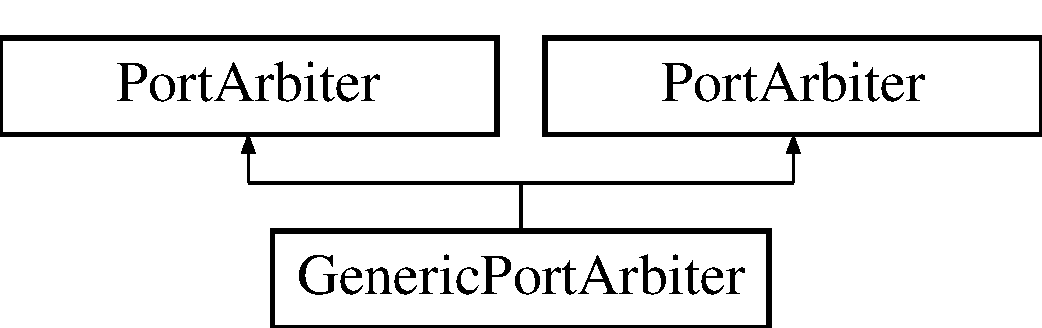
\includegraphics[height=2cm]{classGenericPortArbiter}
\end{center}
\end{figure}
\subsection*{Public Member Functions}
\begin{CompactItemize}
\item 
\hyperlink{classGenericPortArbiter_d7a567eb5055a68231d045583ed8d5a7}{GenericPortArbiter} ()
\item 
\hyperlink{classGenericPortArbiter_2bd7c52f5d2a71863f73f6922520fef8}{$\sim$GenericPortArbiter} ()
\item 
void \hyperlink{classGenericPortArbiter_c4375af1ce810c31e11c03a3b3ffc426}{destroy} ()
\item 
bool \hyperlink{classGenericPortArbiter_a01546e85da0a6d1c1194fbf82f013bb}{is\_\-empty} (\hyperlink{outputBuffer_8h_91ad9478d81a7aaf2593e8d9c3d06a14}{uint} ch)
\item 
void \hyperlink{classGenericPortArbiter_3b94b47628229ee3142907005020eb86}{resize} (\hyperlink{outputBuffer_8h_91ad9478d81a7aaf2593e8d9c3d06a14}{uint} ports)
\item 
void \hyperlink{classGenericPortArbiter_1480ee32b7d8003479d2404a4b279c56}{request} (\hyperlink{classFlit}{Flit} $\ast$f, \hyperlink{outputBuffer_8h_91ad9478d81a7aaf2593e8d9c3d06a14}{uint} port, \hyperlink{outputBuffer_8h_91ad9478d81a7aaf2593e8d9c3d06a14}{uint} vc)
\item 
void \hyperlink{classGenericPortArbiter_50daec6e98669e01d74557dfb84b462f}{set\_\-req\_\-queue\_\-size} (\hyperlink{outputBuffer_8h_91ad9478d81a7aaf2593e8d9c3d06a14}{uint} ch)
\item 
\hyperlink{outputBuffer_8h_91ad9478d81a7aaf2593e8d9c3d06a14}{uint} \hyperlink{classGenericPortArbiter_f58d4de9d0b9e07a44f3f7185f4d11d9}{get\_\-no\_\-requests} ()
\item 
bool \hyperlink{classGenericPortArbiter_b94c8e8e707e00e3265008691fd7c696}{is\_\-requested} (\hyperlink{outputBuffer_8h_91ad9478d81a7aaf2593e8d9c3d06a14}{uint} port, \hyperlink{outputBuffer_8h_91ad9478d81a7aaf2593e8d9c3d06a14}{uint} ch)
\item 
\hyperlink{outputBuffer_8h_91ad9478d81a7aaf2593e8d9c3d06a14}{uint} \hyperlink{classGenericPortArbiter_528c492e74ec10b4ffa2a87d1454b446}{pick\_\-winner} (\hyperlink{outputBuffer_8h_91ad9478d81a7aaf2593e8d9c3d06a14}{uint} ch)
\item 
\hyperlink{classFlit}{Flit} $\ast$ \hyperlink{classGenericPortArbiter_6cc8ecf3ac1cda783e762dc9c139fe01}{pull\_\-winner} (\hyperlink{outputBuffer_8h_91ad9478d81a7aaf2593e8d9c3d06a14}{uint} ch)
\item 
void \hyperlink{classGenericPortArbiter_0ae12cea5cad66f5ef59129e93248e11}{clear} (\hyperlink{outputBuffer_8h_91ad9478d81a7aaf2593e8d9c3d06a14}{uint} ch)
\item 
void \hyperlink{classGenericPortArbiter_63d8b70b6215000469874aa5659cc416}{clear\_\-winner} (\hyperlink{outputBuffer_8h_91ad9478d81a7aaf2593e8d9c3d06a14}{uint} ch)
\item 
vector$<$ \hyperlink{outputBuffer_8h_91ad9478d81a7aaf2593e8d9c3d06a14}{uint} $>$ \hyperlink{classGenericPortArbiter_cd5a78f1bf96701f5371bbcd601d9e53}{get\_\-requests} (\hyperlink{outputBuffer_8h_91ad9478d81a7aaf2593e8d9c3d06a14}{uint} ch)
\item 
string \hyperlink{classGenericPortArbiter_1ceacc98efaee4d98b4f65a401ea10e2}{toString} () const 
\item 
void \hyperlink{classGenericPortArbiter_b593b8edfe4586255c61cb0219f3fb86}{flush\_\-all\_\-requests} ()
\item 
\hyperlink{classGenericPortArbiter_d7a567eb5055a68231d045583ed8d5a7}{GenericPortArbiter} ()
\item 
\hyperlink{classGenericPortArbiter_2bd7c52f5d2a71863f73f6922520fef8}{$\sim$GenericPortArbiter} ()
\item 
void \hyperlink{classGenericPortArbiter_c4375af1ce810c31e11c03a3b3ffc426}{destroy} ()
\item 
bool \hyperlink{classGenericPortArbiter_a01546e85da0a6d1c1194fbf82f013bb}{is\_\-empty} (\hyperlink{outputBuffer_8h_91ad9478d81a7aaf2593e8d9c3d06a14}{uint} ch)
\item 
void \hyperlink{classGenericPortArbiter_3b94b47628229ee3142907005020eb86}{resize} (\hyperlink{outputBuffer_8h_91ad9478d81a7aaf2593e8d9c3d06a14}{uint} ports)
\item 
void \hyperlink{classGenericPortArbiter_1480ee32b7d8003479d2404a4b279c56}{request} (\hyperlink{classFlit}{Flit} $\ast$f, \hyperlink{outputBuffer_8h_91ad9478d81a7aaf2593e8d9c3d06a14}{uint} port, \hyperlink{outputBuffer_8h_91ad9478d81a7aaf2593e8d9c3d06a14}{uint} vc)
\item 
void \hyperlink{classGenericPortArbiter_50daec6e98669e01d74557dfb84b462f}{set\_\-req\_\-queue\_\-size} (\hyperlink{outputBuffer_8h_91ad9478d81a7aaf2593e8d9c3d06a14}{uint} ch)
\item 
\hyperlink{outputBuffer_8h_91ad9478d81a7aaf2593e8d9c3d06a14}{uint} \hyperlink{classGenericPortArbiter_f58d4de9d0b9e07a44f3f7185f4d11d9}{get\_\-no\_\-requests} ()
\item 
bool \hyperlink{classGenericPortArbiter_b94c8e8e707e00e3265008691fd7c696}{is\_\-requested} (\hyperlink{outputBuffer_8h_91ad9478d81a7aaf2593e8d9c3d06a14}{uint} port, \hyperlink{outputBuffer_8h_91ad9478d81a7aaf2593e8d9c3d06a14}{uint} ch)
\item 
\hyperlink{outputBuffer_8h_91ad9478d81a7aaf2593e8d9c3d06a14}{uint} \hyperlink{classGenericPortArbiter_528c492e74ec10b4ffa2a87d1454b446}{pick\_\-winner} (\hyperlink{outputBuffer_8h_91ad9478d81a7aaf2593e8d9c3d06a14}{uint} ch)
\item 
\hyperlink{classFlit}{Flit} $\ast$ \hyperlink{classGenericPortArbiter_443e4f87ec15a53c4381d8870154b74d}{pull\_\-winner} (\hyperlink{outputBuffer_8h_91ad9478d81a7aaf2593e8d9c3d06a14}{uint} ch)
\item 
void \hyperlink{classGenericPortArbiter_0ae12cea5cad66f5ef59129e93248e11}{clear} (\hyperlink{outputBuffer_8h_91ad9478d81a7aaf2593e8d9c3d06a14}{uint} ch)
\item 
void \hyperlink{classGenericPortArbiter_63d8b70b6215000469874aa5659cc416}{clear\_\-winner} (\hyperlink{outputBuffer_8h_91ad9478d81a7aaf2593e8d9c3d06a14}{uint} ch)
\item 
vector$<$ \hyperlink{outputBuffer_8h_91ad9478d81a7aaf2593e8d9c3d06a14}{uint} $>$ \hyperlink{classGenericPortArbiter_cd5a78f1bf96701f5371bbcd601d9e53}{get\_\-requests} (\hyperlink{outputBuffer_8h_91ad9478d81a7aaf2593e8d9c3d06a14}{uint} ch)
\item 
string \hyperlink{classGenericPortArbiter_1ceacc98efaee4d98b4f65a401ea10e2}{toString} () const 
\item 
void \hyperlink{classGenericPortArbiter_b593b8edfe4586255c61cb0219f3fb86}{flush\_\-all\_\-requests} ()
\end{CompactItemize}
\subsection*{Public Attributes}
\begin{CompactItemize}
\item 
unsigned long long int \hyperlink{classGenericPortArbiter_bccdf314a1920de58357e0d2f62f427e}{write\_\-time}
\end{CompactItemize}


\subsection{Constructor \& Destructor Documentation}
\hypertarget{classGenericPortArbiter_d7a567eb5055a68231d045583ed8d5a7}{
\index{GenericPortArbiter@{GenericPortArbiter}!GenericPortArbiter@{GenericPortArbiter}}
\index{GenericPortArbiter@{GenericPortArbiter}!GenericPortArbiter@{GenericPortArbiter}}
\subsubsection[{GenericPortArbiter}]{\setlength{\rightskip}{0pt plus 5cm}GenericPortArbiter::GenericPortArbiter ()}}
\label{classGenericPortArbiter_d7a567eb5055a68231d045583ed8d5a7}


\hypertarget{classGenericPortArbiter_2bd7c52f5d2a71863f73f6922520fef8}{
\index{GenericPortArbiter@{GenericPortArbiter}!$\sim$GenericPortArbiter@{$\sim$GenericPortArbiter}}
\index{$\sim$GenericPortArbiter@{$\sim$GenericPortArbiter}!GenericPortArbiter@{GenericPortArbiter}}
\subsubsection[{$\sim$GenericPortArbiter}]{\setlength{\rightskip}{0pt plus 5cm}GenericPortArbiter::$\sim$GenericPortArbiter ()}}
\label{classGenericPortArbiter_2bd7c52f5d2a71863f73f6922520fef8}


\hypertarget{classGenericPortArbiter_d7a567eb5055a68231d045583ed8d5a7}{
\index{GenericPortArbiter@{GenericPortArbiter}!GenericPortArbiter@{GenericPortArbiter}}
\index{GenericPortArbiter@{GenericPortArbiter}!GenericPortArbiter@{GenericPortArbiter}}
\subsubsection[{GenericPortArbiter}]{\setlength{\rightskip}{0pt plus 5cm}GenericPortArbiter::GenericPortArbiter ()}}
\label{classGenericPortArbiter_d7a567eb5055a68231d045583ed8d5a7}


\hypertarget{classGenericPortArbiter_2bd7c52f5d2a71863f73f6922520fef8}{
\index{GenericPortArbiter@{GenericPortArbiter}!$\sim$GenericPortArbiter@{$\sim$GenericPortArbiter}}
\index{$\sim$GenericPortArbiter@{$\sim$GenericPortArbiter}!GenericPortArbiter@{GenericPortArbiter}}
\subsubsection[{$\sim$GenericPortArbiter}]{\setlength{\rightskip}{0pt plus 5cm}GenericPortArbiter::$\sim$GenericPortArbiter ()}}
\label{classGenericPortArbiter_2bd7c52f5d2a71863f73f6922520fef8}




\subsection{Member Function Documentation}
\hypertarget{classGenericPortArbiter_0ae12cea5cad66f5ef59129e93248e11}{
\index{GenericPortArbiter@{GenericPortArbiter}!clear@{clear}}
\index{clear@{clear}!GenericPortArbiter@{GenericPortArbiter}}
\subsubsection[{clear}]{\setlength{\rightskip}{0pt plus 5cm}void GenericPortArbiter::clear ({\bf uint} {\em ch})}}
\label{classGenericPortArbiter_0ae12cea5cad66f5ef59129e93248e11}


\hypertarget{classGenericPortArbiter_0ae12cea5cad66f5ef59129e93248e11}{
\index{GenericPortArbiter@{GenericPortArbiter}!clear@{clear}}
\index{clear@{clear}!GenericPortArbiter@{GenericPortArbiter}}
\subsubsection[{clear}]{\setlength{\rightskip}{0pt plus 5cm}void GenericPortArbiter::clear ({\bf uint} {\em ch})}}
\label{classGenericPortArbiter_0ae12cea5cad66f5ef59129e93248e11}


\hypertarget{classGenericPortArbiter_63d8b70b6215000469874aa5659cc416}{
\index{GenericPortArbiter@{GenericPortArbiter}!clear\_\-winner@{clear\_\-winner}}
\index{clear\_\-winner@{clear\_\-winner}!GenericPortArbiter@{GenericPortArbiter}}
\subsubsection[{clear\_\-winner}]{\setlength{\rightskip}{0pt plus 5cm}void GenericPortArbiter::clear\_\-winner ({\bf uint} {\em ch})}}
\label{classGenericPortArbiter_63d8b70b6215000469874aa5659cc416}


\hypertarget{classGenericPortArbiter_63d8b70b6215000469874aa5659cc416}{
\index{GenericPortArbiter@{GenericPortArbiter}!clear\_\-winner@{clear\_\-winner}}
\index{clear\_\-winner@{clear\_\-winner}!GenericPortArbiter@{GenericPortArbiter}}
\subsubsection[{clear\_\-winner}]{\setlength{\rightskip}{0pt plus 5cm}void GenericPortArbiter::clear\_\-winner ({\bf uint} {\em ch})}}
\label{classGenericPortArbiter_63d8b70b6215000469874aa5659cc416}


\hypertarget{classGenericPortArbiter_c4375af1ce810c31e11c03a3b3ffc426}{
\index{GenericPortArbiter@{GenericPortArbiter}!destroy@{destroy}}
\index{destroy@{destroy}!GenericPortArbiter@{GenericPortArbiter}}
\subsubsection[{destroy}]{\setlength{\rightskip}{0pt plus 5cm}void GenericPortArbiter::destroy ()}}
\label{classGenericPortArbiter_c4375af1ce810c31e11c03a3b3ffc426}


\hypertarget{classGenericPortArbiter_c4375af1ce810c31e11c03a3b3ffc426}{
\index{GenericPortArbiter@{GenericPortArbiter}!destroy@{destroy}}
\index{destroy@{destroy}!GenericPortArbiter@{GenericPortArbiter}}
\subsubsection[{destroy}]{\setlength{\rightskip}{0pt plus 5cm}void GenericPortArbiter::destroy ()}}
\label{classGenericPortArbiter_c4375af1ce810c31e11c03a3b3ffc426}


\hypertarget{classGenericPortArbiter_b593b8edfe4586255c61cb0219f3fb86}{
\index{GenericPortArbiter@{GenericPortArbiter}!flush\_\-all\_\-requests@{flush\_\-all\_\-requests}}
\index{flush\_\-all\_\-requests@{flush\_\-all\_\-requests}!GenericPortArbiter@{GenericPortArbiter}}
\subsubsection[{flush\_\-all\_\-requests}]{\setlength{\rightskip}{0pt plus 5cm}void GenericPortArbiter::flush\_\-all\_\-requests ()}}
\label{classGenericPortArbiter_b593b8edfe4586255c61cb0219f3fb86}


\hypertarget{classGenericPortArbiter_b593b8edfe4586255c61cb0219f3fb86}{
\index{GenericPortArbiter@{GenericPortArbiter}!flush\_\-all\_\-requests@{flush\_\-all\_\-requests}}
\index{flush\_\-all\_\-requests@{flush\_\-all\_\-requests}!GenericPortArbiter@{GenericPortArbiter}}
\subsubsection[{flush\_\-all\_\-requests}]{\setlength{\rightskip}{0pt plus 5cm}void GenericPortArbiter::flush\_\-all\_\-requests ()}}
\label{classGenericPortArbiter_b593b8edfe4586255c61cb0219f3fb86}


\hypertarget{classGenericPortArbiter_f58d4de9d0b9e07a44f3f7185f4d11d9}{
\index{GenericPortArbiter@{GenericPortArbiter}!get\_\-no\_\-requests@{get\_\-no\_\-requests}}
\index{get\_\-no\_\-requests@{get\_\-no\_\-requests}!GenericPortArbiter@{GenericPortArbiter}}
\subsubsection[{get\_\-no\_\-requests}]{\setlength{\rightskip}{0pt plus 5cm}{\bf uint} GenericPortArbiter::get\_\-no\_\-requests ()}}
\label{classGenericPortArbiter_f58d4de9d0b9e07a44f3f7185f4d11d9}


\hypertarget{classGenericPortArbiter_f58d4de9d0b9e07a44f3f7185f4d11d9}{
\index{GenericPortArbiter@{GenericPortArbiter}!get\_\-no\_\-requests@{get\_\-no\_\-requests}}
\index{get\_\-no\_\-requests@{get\_\-no\_\-requests}!GenericPortArbiter@{GenericPortArbiter}}
\subsubsection[{get\_\-no\_\-requests}]{\setlength{\rightskip}{0pt plus 5cm}{\bf uint} GenericPortArbiter::get\_\-no\_\-requests ()}}
\label{classGenericPortArbiter_f58d4de9d0b9e07a44f3f7185f4d11d9}


\hypertarget{classGenericPortArbiter_cd5a78f1bf96701f5371bbcd601d9e53}{
\index{GenericPortArbiter@{GenericPortArbiter}!get\_\-requests@{get\_\-requests}}
\index{get\_\-requests@{get\_\-requests}!GenericPortArbiter@{GenericPortArbiter}}
\subsubsection[{get\_\-requests}]{\setlength{\rightskip}{0pt plus 5cm}vector$<${\bf uint}$>$ GenericPortArbiter::get\_\-requests ({\bf uint} {\em ch})}}
\label{classGenericPortArbiter_cd5a78f1bf96701f5371bbcd601d9e53}


\hypertarget{classGenericPortArbiter_cd5a78f1bf96701f5371bbcd601d9e53}{
\index{GenericPortArbiter@{GenericPortArbiter}!get\_\-requests@{get\_\-requests}}
\index{get\_\-requests@{get\_\-requests}!GenericPortArbiter@{GenericPortArbiter}}
\subsubsection[{get\_\-requests}]{\setlength{\rightskip}{0pt plus 5cm}vector$<${\bf uint}$>$ GenericPortArbiter::get\_\-requests ({\bf uint} {\em ch})}}
\label{classGenericPortArbiter_cd5a78f1bf96701f5371bbcd601d9e53}


\hypertarget{classGenericPortArbiter_a01546e85da0a6d1c1194fbf82f013bb}{
\index{GenericPortArbiter@{GenericPortArbiter}!is\_\-empty@{is\_\-empty}}
\index{is\_\-empty@{is\_\-empty}!GenericPortArbiter@{GenericPortArbiter}}
\subsubsection[{is\_\-empty}]{\setlength{\rightskip}{0pt plus 5cm}bool GenericPortArbiter::is\_\-empty ({\bf uint} {\em ch})}}
\label{classGenericPortArbiter_a01546e85da0a6d1c1194fbf82f013bb}


\hypertarget{classGenericPortArbiter_a01546e85da0a6d1c1194fbf82f013bb}{
\index{GenericPortArbiter@{GenericPortArbiter}!is\_\-empty@{is\_\-empty}}
\index{is\_\-empty@{is\_\-empty}!GenericPortArbiter@{GenericPortArbiter}}
\subsubsection[{is\_\-empty}]{\setlength{\rightskip}{0pt plus 5cm}bool GenericPortArbiter::is\_\-empty ({\bf uint} {\em ch})}}
\label{classGenericPortArbiter_a01546e85da0a6d1c1194fbf82f013bb}


\hypertarget{classGenericPortArbiter_b94c8e8e707e00e3265008691fd7c696}{
\index{GenericPortArbiter@{GenericPortArbiter}!is\_\-requested@{is\_\-requested}}
\index{is\_\-requested@{is\_\-requested}!GenericPortArbiter@{GenericPortArbiter}}
\subsubsection[{is\_\-requested}]{\setlength{\rightskip}{0pt plus 5cm}bool GenericPortArbiter::is\_\-requested ({\bf uint} {\em port}, \/  {\bf uint} {\em ch})}}
\label{classGenericPortArbiter_b94c8e8e707e00e3265008691fd7c696}


\hypertarget{classGenericPortArbiter_b94c8e8e707e00e3265008691fd7c696}{
\index{GenericPortArbiter@{GenericPortArbiter}!is\_\-requested@{is\_\-requested}}
\index{is\_\-requested@{is\_\-requested}!GenericPortArbiter@{GenericPortArbiter}}
\subsubsection[{is\_\-requested}]{\setlength{\rightskip}{0pt plus 5cm}bool GenericPortArbiter::is\_\-requested ({\bf uint} {\em port}, \/  {\bf uint} {\em ch})}}
\label{classGenericPortArbiter_b94c8e8e707e00e3265008691fd7c696}


\hypertarget{classGenericPortArbiter_528c492e74ec10b4ffa2a87d1454b446}{
\index{GenericPortArbiter@{GenericPortArbiter}!pick\_\-winner@{pick\_\-winner}}
\index{pick\_\-winner@{pick\_\-winner}!GenericPortArbiter@{GenericPortArbiter}}
\subsubsection[{pick\_\-winner}]{\setlength{\rightskip}{0pt plus 5cm}{\bf uint} GenericPortArbiter::pick\_\-winner ({\bf uint} {\em ch})}}
\label{classGenericPortArbiter_528c492e74ec10b4ffa2a87d1454b446}


\hypertarget{classGenericPortArbiter_528c492e74ec10b4ffa2a87d1454b446}{
\index{GenericPortArbiter@{GenericPortArbiter}!pick\_\-winner@{pick\_\-winner}}
\index{pick\_\-winner@{pick\_\-winner}!GenericPortArbiter@{GenericPortArbiter}}
\subsubsection[{pick\_\-winner}]{\setlength{\rightskip}{0pt plus 5cm}{\bf uint} GenericPortArbiter::pick\_\-winner ({\bf uint} {\em ch})}}
\label{classGenericPortArbiter_528c492e74ec10b4ffa2a87d1454b446}


\hypertarget{classGenericPortArbiter_443e4f87ec15a53c4381d8870154b74d}{
\index{GenericPortArbiter@{GenericPortArbiter}!pull\_\-winner@{pull\_\-winner}}
\index{pull\_\-winner@{pull\_\-winner}!GenericPortArbiter@{GenericPortArbiter}}
\subsubsection[{pull\_\-winner}]{\setlength{\rightskip}{0pt plus 5cm}{\bf Flit}$\ast$ GenericPortArbiter::pull\_\-winner ({\bf uint} {\em ch})}}
\label{classGenericPortArbiter_443e4f87ec15a53c4381d8870154b74d}


\hypertarget{classGenericPortArbiter_6cc8ecf3ac1cda783e762dc9c139fe01}{
\index{GenericPortArbiter@{GenericPortArbiter}!pull\_\-winner@{pull\_\-winner}}
\index{pull\_\-winner@{pull\_\-winner}!GenericPortArbiter@{GenericPortArbiter}}
\subsubsection[{pull\_\-winner}]{\setlength{\rightskip}{0pt plus 5cm}{\bf Flit} $\ast$ GenericPortArbiter::pull\_\-winner ({\bf uint} {\em ch})}}
\label{classGenericPortArbiter_6cc8ecf3ac1cda783e762dc9c139fe01}


\hypertarget{classGenericPortArbiter_1480ee32b7d8003479d2404a4b279c56}{
\index{GenericPortArbiter@{GenericPortArbiter}!request@{request}}
\index{request@{request}!GenericPortArbiter@{GenericPortArbiter}}
\subsubsection[{request}]{\setlength{\rightskip}{0pt plus 5cm}void GenericPortArbiter::request ({\bf Flit} $\ast$ {\em f}, \/  {\bf uint} {\em port}, \/  {\bf uint} {\em vc})}}
\label{classGenericPortArbiter_1480ee32b7d8003479d2404a4b279c56}


\hypertarget{classGenericPortArbiter_1480ee32b7d8003479d2404a4b279c56}{
\index{GenericPortArbiter@{GenericPortArbiter}!request@{request}}
\index{request@{request}!GenericPortArbiter@{GenericPortArbiter}}
\subsubsection[{request}]{\setlength{\rightskip}{0pt plus 5cm}void GenericPortArbiter::request ({\bf Flit} $\ast$ {\em f}, \/  {\bf uint} {\em port}, \/  {\bf uint} {\em vc})}}
\label{classGenericPortArbiter_1480ee32b7d8003479d2404a4b279c56}


\hypertarget{classGenericPortArbiter_3b94b47628229ee3142907005020eb86}{
\index{GenericPortArbiter@{GenericPortArbiter}!resize@{resize}}
\index{resize@{resize}!GenericPortArbiter@{GenericPortArbiter}}
\subsubsection[{resize}]{\setlength{\rightskip}{0pt plus 5cm}void GenericPortArbiter::resize ({\bf uint} {\em ports})}}
\label{classGenericPortArbiter_3b94b47628229ee3142907005020eb86}


\hypertarget{classGenericPortArbiter_3b94b47628229ee3142907005020eb86}{
\index{GenericPortArbiter@{GenericPortArbiter}!resize@{resize}}
\index{resize@{resize}!GenericPortArbiter@{GenericPortArbiter}}
\subsubsection[{resize}]{\setlength{\rightskip}{0pt plus 5cm}void GenericPortArbiter::resize ({\bf uint} {\em ports})}}
\label{classGenericPortArbiter_3b94b47628229ee3142907005020eb86}


\hypertarget{classGenericPortArbiter_50daec6e98669e01d74557dfb84b462f}{
\index{GenericPortArbiter@{GenericPortArbiter}!set\_\-req\_\-queue\_\-size@{set\_\-req\_\-queue\_\-size}}
\index{set\_\-req\_\-queue\_\-size@{set\_\-req\_\-queue\_\-size}!GenericPortArbiter@{GenericPortArbiter}}
\subsubsection[{set\_\-req\_\-queue\_\-size}]{\setlength{\rightskip}{0pt plus 5cm}void GenericPortArbiter::set\_\-req\_\-queue\_\-size ({\bf uint} {\em ch})}}
\label{classGenericPortArbiter_50daec6e98669e01d74557dfb84b462f}


\hypertarget{classGenericPortArbiter_50daec6e98669e01d74557dfb84b462f}{
\index{GenericPortArbiter@{GenericPortArbiter}!set\_\-req\_\-queue\_\-size@{set\_\-req\_\-queue\_\-size}}
\index{set\_\-req\_\-queue\_\-size@{set\_\-req\_\-queue\_\-size}!GenericPortArbiter@{GenericPortArbiter}}
\subsubsection[{set\_\-req\_\-queue\_\-size}]{\setlength{\rightskip}{0pt plus 5cm}void GenericPortArbiter::set\_\-req\_\-queue\_\-size ({\bf uint} {\em ch})}}
\label{classGenericPortArbiter_50daec6e98669e01d74557dfb84b462f}


\hypertarget{classGenericPortArbiter_1ceacc98efaee4d98b4f65a401ea10e2}{
\index{GenericPortArbiter@{GenericPortArbiter}!toString@{toString}}
\index{toString@{toString}!GenericPortArbiter@{GenericPortArbiter}}
\subsubsection[{toString}]{\setlength{\rightskip}{0pt plus 5cm}string GenericPortArbiter::toString () const}}
\label{classGenericPortArbiter_1ceacc98efaee4d98b4f65a401ea10e2}


\hypertarget{classGenericPortArbiter_1ceacc98efaee4d98b4f65a401ea10e2}{
\index{GenericPortArbiter@{GenericPortArbiter}!toString@{toString}}
\index{toString@{toString}!GenericPortArbiter@{GenericPortArbiter}}
\subsubsection[{toString}]{\setlength{\rightskip}{0pt plus 5cm}string GenericPortArbiter::toString () const}}
\label{classGenericPortArbiter_1ceacc98efaee4d98b4f65a401ea10e2}




\subsection{Member Data Documentation}
\hypertarget{classGenericPortArbiter_bccdf314a1920de58357e0d2f62f427e}{
\index{GenericPortArbiter@{GenericPortArbiter}!write\_\-time@{write\_\-time}}
\index{write\_\-time@{write\_\-time}!GenericPortArbiter@{GenericPortArbiter}}
\subsubsection[{write\_\-time}]{\setlength{\rightskip}{0pt plus 5cm}unsigned long long int {\bf GenericPortArbiter::write\_\-time}}}
\label{classGenericPortArbiter_bccdf314a1920de58357e0d2f62f427e}




The documentation for this class was generated from the following files:\begin{CompactItemize}
\item 
source/components/impl/backup/\hyperlink{impl_2backup_2genericPortArbiter_8h}{genericPortArbiter.h}\item 
source/components/none/\hyperlink{none_2genericPortArbiter_8h}{genericPortArbiter.h}\item 
source/components/impl/backup/\hyperlink{impl_2backup_2genericPortArbiter_8cc}{genericPortArbiter.cc}\item 
source/components/none/\hyperlink{none_2genericPortArbiter_8cc}{genericPortArbiter.cc}\end{CompactItemize}

\hypertarget{classGenericRC}{
\section{GenericRC Class Reference}
\label{classGenericRC}\index{GenericRC@{GenericRC}}
}
{\tt \#include $<$genericRC.h$>$}

\subsection*{Classes}
\begin{CompactItemize}
\item 
class \textbf{Address}
\end{CompactItemize}
\subsection*{Public Member Functions}
\begin{CompactItemize}
\item 
\hyperlink{classGenericRC_92f9cd6b1dafc9eb0a3a1450448888fe}{GenericRC} ()
\item 
\hyperlink{classGenericRC_f63422fabc3b4393e060ea7ad68981e9}{$\sim$GenericRC} ()
\item 
void \hyperlink{classGenericRC_4698476460f0a811482905dbab564764}{push} (\hyperlink{classFlit}{Flit} $\ast$f, unsigned int vc)
\item 
unsigned int \hyperlink{classGenericRC_75ca57d2ed84543ef4083c2fe8e83644}{get\_\-output\_\-port} (unsigned int channel)
\item 
unsigned int \hyperlink{classGenericRC_23666c0b23e511d1f46917023fe26b66}{speculate\_\-port} (\hyperlink{classFlit}{Flit} $\ast$f, unsigned int ch)
\item 
unsigned int \hyperlink{classGenericRC_62380900287660d9e73a80f8da7800ab}{speculate\_\-channel} (\hyperlink{classFlit}{Flit} $\ast$f, unsigned int ch)
\item 
unsigned int \hyperlink{classGenericRC_c311af5e27b084df2e2463b74e207e3f}{get\_\-virtual\_\-channel} (unsigned int ch)
\item 
void \hyperlink{classGenericRC_611a7de2bb3f1eeea039185f706d0745}{resize} (unsigned int ch)
\item 
unsigned int \hyperlink{classGenericRC_6d8e1133e7eefd95a25a4dfe7d45491e}{get\_\-no\_\-channels} ()
\item 
bool \hyperlink{classGenericRC_5fc891e7753c5e06cd3599b11bab60a6}{is\_\-empty} ()
\item 
string \hyperlink{classGenericRC_214ef51af1dd900b41bb98b4826b5af4}{toString} () const 
\end{CompactItemize}
\subsection*{Public Attributes}
\begin{CompactItemize}
\item 
\hyperlink{outputBuffer_8h_91ad9478d81a7aaf2593e8d9c3d06a14}{uint} \hyperlink{classGenericRC_f937d0d5d2df92a5be2641fb062f312e}{node\_\-ip}
\item 
\hyperlink{outputBuffer_8h_91ad9478d81a7aaf2593e8d9c3d06a14}{uint} \hyperlink{classGenericRC_5a89c8b3e742b017f108ce1075422526}{address}
\item 
vector$<$ \hyperlink{outputBuffer_8h_91ad9478d81a7aaf2593e8d9c3d06a14}{uint} $>$ \hyperlink{classGenericRC_2e2f02ddede7cfafca6073ee559663e2}{grid\_\-xloc}
\item 
vector$<$ \hyperlink{outputBuffer_8h_91ad9478d81a7aaf2593e8d9c3d06a14}{uint} $>$ \hyperlink{classGenericRC_89b5f8d2de4dc45ce64cbb0038ec0efa}{grid\_\-yloc}
\end{CompactItemize}


\subsection{Constructor \& Destructor Documentation}
\hypertarget{classGenericRC_92f9cd6b1dafc9eb0a3a1450448888fe}{
\index{GenericRC@{GenericRC}!GenericRC@{GenericRC}}
\index{GenericRC@{GenericRC}!GenericRC@{GenericRC}}
\subsubsection[{GenericRC}]{\setlength{\rightskip}{0pt plus 5cm}GenericRC::GenericRC ()}}
\label{classGenericRC_92f9cd6b1dafc9eb0a3a1450448888fe}


\hypertarget{classGenericRC_f63422fabc3b4393e060ea7ad68981e9}{
\index{GenericRC@{GenericRC}!$\sim$GenericRC@{$\sim$GenericRC}}
\index{$\sim$GenericRC@{$\sim$GenericRC}!GenericRC@{GenericRC}}
\subsubsection[{$\sim$GenericRC}]{\setlength{\rightskip}{0pt plus 5cm}GenericRC::$\sim$GenericRC ()\hspace{0.3cm}{\tt  \mbox{[}inline\mbox{]}}}}
\label{classGenericRC_f63422fabc3b4393e060ea7ad68981e9}




\subsection{Member Function Documentation}
\hypertarget{classGenericRC_6d8e1133e7eefd95a25a4dfe7d45491e}{
\index{GenericRC@{GenericRC}!get\_\-no\_\-channels@{get\_\-no\_\-channels}}
\index{get\_\-no\_\-channels@{get\_\-no\_\-channels}!GenericRC@{GenericRC}}
\subsubsection[{get\_\-no\_\-channels}]{\setlength{\rightskip}{0pt plus 5cm}{\bf uint} GenericRC::get\_\-no\_\-channels ()}}
\label{classGenericRC_6d8e1133e7eefd95a25a4dfe7d45491e}


\hypertarget{classGenericRC_75ca57d2ed84543ef4083c2fe8e83644}{
\index{GenericRC@{GenericRC}!get\_\-output\_\-port@{get\_\-output\_\-port}}
\index{get\_\-output\_\-port@{get\_\-output\_\-port}!GenericRC@{GenericRC}}
\subsubsection[{get\_\-output\_\-port}]{\setlength{\rightskip}{0pt plus 5cm}{\bf uint} GenericRC::get\_\-output\_\-port (unsigned int {\em channel})}}
\label{classGenericRC_75ca57d2ed84543ef4083c2fe8e83644}


\hypertarget{classGenericRC_c311af5e27b084df2e2463b74e207e3f}{
\index{GenericRC@{GenericRC}!get\_\-virtual\_\-channel@{get\_\-virtual\_\-channel}}
\index{get\_\-virtual\_\-channel@{get\_\-virtual\_\-channel}!GenericRC@{GenericRC}}
\subsubsection[{get\_\-virtual\_\-channel}]{\setlength{\rightskip}{0pt plus 5cm}{\bf uint} GenericRC::get\_\-virtual\_\-channel (unsigned int {\em ch})}}
\label{classGenericRC_c311af5e27b084df2e2463b74e207e3f}


\hypertarget{classGenericRC_5fc891e7753c5e06cd3599b11bab60a6}{
\index{GenericRC@{GenericRC}!is\_\-empty@{is\_\-empty}}
\index{is\_\-empty@{is\_\-empty}!GenericRC@{GenericRC}}
\subsubsection[{is\_\-empty}]{\setlength{\rightskip}{0pt plus 5cm}bool GenericRC::is\_\-empty ()}}
\label{classGenericRC_5fc891e7753c5e06cd3599b11bab60a6}


\hypertarget{classGenericRC_4698476460f0a811482905dbab564764}{
\index{GenericRC@{GenericRC}!push@{push}}
\index{push@{push}!GenericRC@{GenericRC}}
\subsubsection[{push}]{\setlength{\rightskip}{0pt plus 5cm}void GenericRC::push ({\bf Flit} $\ast$ {\em f}, \/  unsigned int {\em vc})}}
\label{classGenericRC_4698476460f0a811482905dbab564764}


\hypertarget{classGenericRC_611a7de2bb3f1eeea039185f706d0745}{
\index{GenericRC@{GenericRC}!resize@{resize}}
\index{resize@{resize}!GenericRC@{GenericRC}}
\subsubsection[{resize}]{\setlength{\rightskip}{0pt plus 5cm}void GenericRC::resize (unsigned int {\em ch})}}
\label{classGenericRC_611a7de2bb3f1eeea039185f706d0745}


\hypertarget{classGenericRC_62380900287660d9e73a80f8da7800ab}{
\index{GenericRC@{GenericRC}!speculate\_\-channel@{speculate\_\-channel}}
\index{speculate\_\-channel@{speculate\_\-channel}!GenericRC@{GenericRC}}
\subsubsection[{speculate\_\-channel}]{\setlength{\rightskip}{0pt plus 5cm}unsigned int GenericRC::speculate\_\-channel ({\bf Flit} $\ast$ {\em f}, \/  unsigned int {\em ch})}}
\label{classGenericRC_62380900287660d9e73a80f8da7800ab}


\hypertarget{classGenericRC_23666c0b23e511d1f46917023fe26b66}{
\index{GenericRC@{GenericRC}!speculate\_\-port@{speculate\_\-port}}
\index{speculate\_\-port@{speculate\_\-port}!GenericRC@{GenericRC}}
\subsubsection[{speculate\_\-port}]{\setlength{\rightskip}{0pt plus 5cm}unsigned int GenericRC::speculate\_\-port ({\bf Flit} $\ast$ {\em f}, \/  unsigned int {\em ch})}}
\label{classGenericRC_23666c0b23e511d1f46917023fe26b66}


\hypertarget{classGenericRC_214ef51af1dd900b41bb98b4826b5af4}{
\index{GenericRC@{GenericRC}!toString@{toString}}
\index{toString@{toString}!GenericRC@{GenericRC}}
\subsubsection[{toString}]{\setlength{\rightskip}{0pt plus 5cm}string GenericRC::toString () const}}
\label{classGenericRC_214ef51af1dd900b41bb98b4826b5af4}




\subsection{Member Data Documentation}
\hypertarget{classGenericRC_5a89c8b3e742b017f108ce1075422526}{
\index{GenericRC@{GenericRC}!address@{address}}
\index{address@{address}!GenericRC@{GenericRC}}
\subsubsection[{address}]{\setlength{\rightskip}{0pt plus 5cm}{\bf uint} {\bf GenericRC::address}}}
\label{classGenericRC_5a89c8b3e742b017f108ce1075422526}


\hypertarget{classGenericRC_2e2f02ddede7cfafca6073ee559663e2}{
\index{GenericRC@{GenericRC}!grid\_\-xloc@{grid\_\-xloc}}
\index{grid\_\-xloc@{grid\_\-xloc}!GenericRC@{GenericRC}}
\subsubsection[{grid\_\-xloc}]{\setlength{\rightskip}{0pt plus 5cm}vector$<$ {\bf uint} $>$ {\bf GenericRC::grid\_\-xloc}}}
\label{classGenericRC_2e2f02ddede7cfafca6073ee559663e2}


\hypertarget{classGenericRC_89b5f8d2de4dc45ce64cbb0038ec0efa}{
\index{GenericRC@{GenericRC}!grid\_\-yloc@{grid\_\-yloc}}
\index{grid\_\-yloc@{grid\_\-yloc}!GenericRC@{GenericRC}}
\subsubsection[{grid\_\-yloc}]{\setlength{\rightskip}{0pt plus 5cm}vector$<$ {\bf uint} $>$ {\bf GenericRC::grid\_\-yloc}}}
\label{classGenericRC_89b5f8d2de4dc45ce64cbb0038ec0efa}


\hypertarget{classGenericRC_f937d0d5d2df92a5be2641fb062f312e}{
\index{GenericRC@{GenericRC}!node\_\-ip@{node\_\-ip}}
\index{node\_\-ip@{node\_\-ip}!GenericRC@{GenericRC}}
\subsubsection[{node\_\-ip}]{\setlength{\rightskip}{0pt plus 5cm}{\bf uint} {\bf GenericRC::node\_\-ip}}}
\label{classGenericRC_f937d0d5d2df92a5be2641fb062f312e}




The documentation for this class was generated from the following files:\begin{CompactItemize}
\item 
source/components/impl/\hyperlink{genericRC_8h}{genericRC.h}\item 
source/components/impl/\hyperlink{genericRC_8cc}{genericRC.cc}\end{CompactItemize}

\hypertarget{classGenericRouterNoVcs}{
\section{GenericRouterNoVcs Class Reference}
\label{classGenericRouterNoVcs}\index{GenericRouterNoVcs@{GenericRouterNoVcs}}
}
{\tt \#include $<$genericRouterNoVcs.h$>$}

Inheritance diagram for GenericRouterNoVcs::\begin{figure}[H]
\begin{center}
\leavevmode
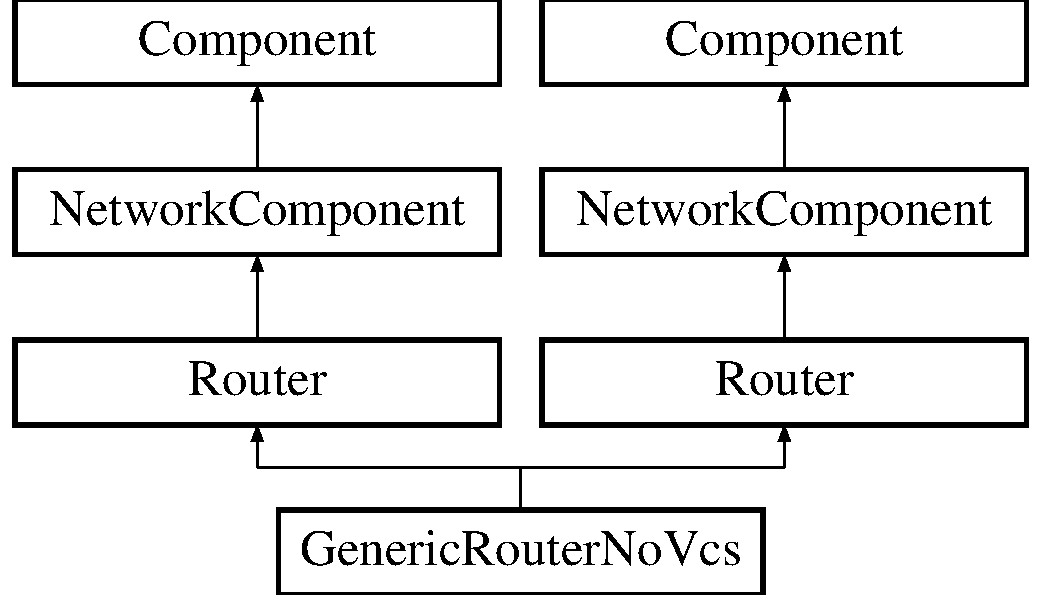
\includegraphics[height=4cm]{classGenericRouterNoVcs}
\end{center}
\end{figure}
\subsection*{Public Member Functions}
\begin{CompactItemize}
\item 
\hyperlink{classGenericRouterNoVcs_0c9d450ec65aa82e1f82d20b3d7c66e1}{GenericRouterNoVcs} ()
\item 
\hyperlink{classGenericRouterNoVcs_25aa63b54decdffddb9bfd2da7759c4b}{$\sim$GenericRouterNoVcs} ()
\item 
void \hyperlink{classGenericRouterNoVcs_d0abf72a39438d7b23b9b03029d75da2}{init} (\hyperlink{outputBuffer_8h_91ad9478d81a7aaf2593e8d9c3d06a14}{uint} \hyperlink{classRouter_fd8e8adaf03e17b3fdbf7adc758c8f48}{ports}, \hyperlink{outputBuffer_8h_91ad9478d81a7aaf2593e8d9c3d06a14}{uint} \hyperlink{classRouter_ebaf2bc63bd99effe6520f9718120a1e}{vcs}, \hyperlink{outputBuffer_8h_91ad9478d81a7aaf2593e8d9c3d06a14}{uint} \hyperlink{classRouter_d747f5b948a9ef1497de6d4bb97b8f03}{credits}, \hyperlink{outputBuffer_8h_91ad9478d81a7aaf2593e8d9c3d06a14}{uint} \hyperlink{classRouter_b456618374083b8f2ec3c8e889d45bac}{buffer\_\-size})
\item 
void \hyperlink{classGenericRouterNoVcs_877a1b3fac555ef48ad7690429b2be28}{set\_\-no\_\-nodes} (\hyperlink{outputBuffer_8h_91ad9478d81a7aaf2593e8d9c3d06a14}{uint} nodes)
\begin{CompactList}\small\item\em These functions are mainly for DOR routing and are seperated so as to not force DOR modelling in all designs. \item\end{CompactList}\item 
void \hyperlink{classGenericRouterNoVcs_9a0bc9c779518e5564bb25c0a3867434}{set\_\-grid\_\-x\_\-location} (\hyperlink{outputBuffer_8h_91ad9478d81a7aaf2593e8d9c3d06a14}{uint} a, \hyperlink{outputBuffer_8h_91ad9478d81a7aaf2593e8d9c3d06a14}{uint} b, \hyperlink{outputBuffer_8h_91ad9478d81a7aaf2593e8d9c3d06a14}{uint} c)
\item 
void \hyperlink{classGenericRouterNoVcs_30fb743466538fcf9d158ffa665f9ca2}{set\_\-grid\_\-y\_\-location} (\hyperlink{outputBuffer_8h_91ad9478d81a7aaf2593e8d9c3d06a14}{uint} a, \hyperlink{outputBuffer_8h_91ad9478d81a7aaf2593e8d9c3d06a14}{uint} b, \hyperlink{outputBuffer_8h_91ad9478d81a7aaf2593e8d9c3d06a14}{uint} c)
\item 
void \hyperlink{classGenericRouterNoVcs_f8bd205f15bb6ef680e1af859950f3d9}{send\_\-credit\_\-back} (\hyperlink{outputBuffer_8h_91ad9478d81a7aaf2593e8d9c3d06a14}{uint} i)
\item 
void \hyperlink{classGenericRouterNoVcs_a2c52d53e127c9a3a029194e77f9f80c}{process\_\-event} (\hyperlink{classIrisEvent}{IrisEvent} $\ast$e)
\item 
string \hyperlink{classGenericRouterNoVcs_59307c319fbca5732d750630be9ee27c}{toString} () const 
\item 
string \hyperlink{classGenericRouterNoVcs_897a642767b5ecf17ec45220d201b7e6}{print\_\-stats} ()
\item 
\hyperlink{classGenericRouterNoVcs_0c9d450ec65aa82e1f82d20b3d7c66e1}{GenericRouterNoVcs} ()
\item 
\hyperlink{classGenericRouterNoVcs_25aa63b54decdffddb9bfd2da7759c4b}{$\sim$GenericRouterNoVcs} ()
\item 
void \hyperlink{classGenericRouterNoVcs_d0abf72a39438d7b23b9b03029d75da2}{init} (\hyperlink{outputBuffer_8h_91ad9478d81a7aaf2593e8d9c3d06a14}{uint} \hyperlink{classRouter_fd8e8adaf03e17b3fdbf7adc758c8f48}{ports}, \hyperlink{outputBuffer_8h_91ad9478d81a7aaf2593e8d9c3d06a14}{uint} \hyperlink{classRouter_ebaf2bc63bd99effe6520f9718120a1e}{vcs}, \hyperlink{outputBuffer_8h_91ad9478d81a7aaf2593e8d9c3d06a14}{uint} \hyperlink{classRouter_d747f5b948a9ef1497de6d4bb97b8f03}{credits}, \hyperlink{outputBuffer_8h_91ad9478d81a7aaf2593e8d9c3d06a14}{uint} \hyperlink{classRouter_b456618374083b8f2ec3c8e889d45bac}{buffer\_\-size})
\item 
void \hyperlink{classGenericRouterNoVcs_877a1b3fac555ef48ad7690429b2be28}{set\_\-no\_\-nodes} (\hyperlink{outputBuffer_8h_91ad9478d81a7aaf2593e8d9c3d06a14}{uint} nodes)
\item 
void \hyperlink{classGenericRouterNoVcs_9a0bc9c779518e5564bb25c0a3867434}{set\_\-grid\_\-x\_\-location} (\hyperlink{outputBuffer_8h_91ad9478d81a7aaf2593e8d9c3d06a14}{uint} a, \hyperlink{outputBuffer_8h_91ad9478d81a7aaf2593e8d9c3d06a14}{uint} b, \hyperlink{outputBuffer_8h_91ad9478d81a7aaf2593e8d9c3d06a14}{uint} c)
\item 
void \hyperlink{classGenericRouterNoVcs_30fb743466538fcf9d158ffa665f9ca2}{set\_\-grid\_\-y\_\-location} (\hyperlink{outputBuffer_8h_91ad9478d81a7aaf2593e8d9c3d06a14}{uint} a, \hyperlink{outputBuffer_8h_91ad9478d81a7aaf2593e8d9c3d06a14}{uint} b, \hyperlink{outputBuffer_8h_91ad9478d81a7aaf2593e8d9c3d06a14}{uint} c)
\item 
void \hyperlink{classGenericRouterNoVcs_f8bd205f15bb6ef680e1af859950f3d9}{send\_\-credit\_\-back} (\hyperlink{outputBuffer_8h_91ad9478d81a7aaf2593e8d9c3d06a14}{uint} i)
\item 
void \hyperlink{classGenericRouterNoVcs_a2c52d53e127c9a3a029194e77f9f80c}{process\_\-event} (\hyperlink{classIrisEvent}{IrisEvent} $\ast$e)
\item 
string \hyperlink{classGenericRouterNoVcs_59307c319fbca5732d750630be9ee27c}{toString} () const 
\item 
string \hyperlink{classGenericRouterNoVcs_897a642767b5ecf17ec45220d201b7e6}{print\_\-stats} ()
\end{CompactItemize}
\subsection*{Public Attributes}
\begin{CompactItemize}
\item 
vector$<$ vector$<$ \hyperlink{outputBuffer_8h_91ad9478d81a7aaf2593e8d9c3d06a14}{uint} $>$ $>$ \hyperlink{classGenericRouterNoVcs_ee50aef2694512a3fdbceca9f5fe8b7e}{downstream\_\-credits}
\item 
\hyperlink{outputBuffer_8h_91ad9478d81a7aaf2593e8d9c3d06a14}{uint} \hyperlink{classGenericRouterNoVcs_dba7f3303be476622b197de24f8b4424}{packets}
\item 
\hyperlink{outputBuffer_8h_91ad9478d81a7aaf2593e8d9c3d06a14}{uint} \hyperlink{classGenericRouterNoVcs_f1f16a8fee993cd6287c8772300c1936}{flits}
\item 
double \hyperlink{classGenericRouterNoVcs_e0c46058ebe12608d9149609ca33e142}{total\_\-packet\_\-latency}
\item 
double \hyperlink{classGenericRouterNoVcs_9dcc34984deb05947a392e063b4eb718}{last\_\-flit\_\-out\_\-cycle}
\end{CompactItemize}


\subsection{Constructor \& Destructor Documentation}
\hypertarget{classGenericRouterNoVcs_0c9d450ec65aa82e1f82d20b3d7c66e1}{
\index{GenericRouterNoVcs@{GenericRouterNoVcs}!GenericRouterNoVcs@{GenericRouterNoVcs}}
\index{GenericRouterNoVcs@{GenericRouterNoVcs}!GenericRouterNoVcs@{GenericRouterNoVcs}}
\subsubsection[{GenericRouterNoVcs}]{\setlength{\rightskip}{0pt plus 5cm}GenericRouterNoVcs::GenericRouterNoVcs ()}}
\label{classGenericRouterNoVcs_0c9d450ec65aa82e1f82d20b3d7c66e1}


\hypertarget{classGenericRouterNoVcs_25aa63b54decdffddb9bfd2da7759c4b}{
\index{GenericRouterNoVcs@{GenericRouterNoVcs}!$\sim$GenericRouterNoVcs@{$\sim$GenericRouterNoVcs}}
\index{$\sim$GenericRouterNoVcs@{$\sim$GenericRouterNoVcs}!GenericRouterNoVcs@{GenericRouterNoVcs}}
\subsubsection[{$\sim$GenericRouterNoVcs}]{\setlength{\rightskip}{0pt plus 5cm}GenericRouterNoVcs::$\sim$GenericRouterNoVcs ()}}
\label{classGenericRouterNoVcs_25aa63b54decdffddb9bfd2da7759c4b}


\hypertarget{classGenericRouterNoVcs_0c9d450ec65aa82e1f82d20b3d7c66e1}{
\index{GenericRouterNoVcs@{GenericRouterNoVcs}!GenericRouterNoVcs@{GenericRouterNoVcs}}
\index{GenericRouterNoVcs@{GenericRouterNoVcs}!GenericRouterNoVcs@{GenericRouterNoVcs}}
\subsubsection[{GenericRouterNoVcs}]{\setlength{\rightskip}{0pt plus 5cm}GenericRouterNoVcs::GenericRouterNoVcs ()}}
\label{classGenericRouterNoVcs_0c9d450ec65aa82e1f82d20b3d7c66e1}


\hypertarget{classGenericRouterNoVcs_25aa63b54decdffddb9bfd2da7759c4b}{
\index{GenericRouterNoVcs@{GenericRouterNoVcs}!$\sim$GenericRouterNoVcs@{$\sim$GenericRouterNoVcs}}
\index{$\sim$GenericRouterNoVcs@{$\sim$GenericRouterNoVcs}!GenericRouterNoVcs@{GenericRouterNoVcs}}
\subsubsection[{$\sim$GenericRouterNoVcs}]{\setlength{\rightskip}{0pt plus 5cm}GenericRouterNoVcs::$\sim$GenericRouterNoVcs ()}}
\label{classGenericRouterNoVcs_25aa63b54decdffddb9bfd2da7759c4b}




\subsection{Member Function Documentation}
\hypertarget{classGenericRouterNoVcs_d0abf72a39438d7b23b9b03029d75da2}{
\index{GenericRouterNoVcs@{GenericRouterNoVcs}!init@{init}}
\index{init@{init}!GenericRouterNoVcs@{GenericRouterNoVcs}}
\subsubsection[{init}]{\setlength{\rightskip}{0pt plus 5cm}void GenericRouterNoVcs::init ({\bf uint} {\em ports}, \/  {\bf uint} {\em vcs}, \/  {\bf uint} {\em credits}, \/  {\bf uint} {\em buffer\_\-size})\hspace{0.3cm}{\tt  \mbox{[}virtual\mbox{]}}}}
\label{classGenericRouterNoVcs_d0abf72a39438d7b23b9b03029d75da2}




Implements \hyperlink{classRouter_7c551f11fcda9accb02da87c671c4065}{Router}.\hypertarget{classGenericRouterNoVcs_d0abf72a39438d7b23b9b03029d75da2}{
\index{GenericRouterNoVcs@{GenericRouterNoVcs}!init@{init}}
\index{init@{init}!GenericRouterNoVcs@{GenericRouterNoVcs}}
\subsubsection[{init}]{\setlength{\rightskip}{0pt plus 5cm}void GenericRouterNoVcs::init ({\bf uint} {\em ports}, \/  {\bf uint} {\em vcs}, \/  {\bf uint} {\em credits}, \/  {\bf uint} {\em buffer\_\-size})\hspace{0.3cm}{\tt  \mbox{[}virtual\mbox{]}}}}
\label{classGenericRouterNoVcs_d0abf72a39438d7b23b9b03029d75da2}




Implements \hyperlink{classRouter_7c551f11fcda9accb02da87c671c4065}{Router}.\hypertarget{classGenericRouterNoVcs_897a642767b5ecf17ec45220d201b7e6}{
\index{GenericRouterNoVcs@{GenericRouterNoVcs}!print\_\-stats@{print\_\-stats}}
\index{print\_\-stats@{print\_\-stats}!GenericRouterNoVcs@{GenericRouterNoVcs}}
\subsubsection[{print\_\-stats}]{\setlength{\rightskip}{0pt plus 5cm}string GenericRouterNoVcs::print\_\-stats ()\hspace{0.3cm}{\tt  \mbox{[}virtual\mbox{]}}}}
\label{classGenericRouterNoVcs_897a642767b5ecf17ec45220d201b7e6}




Implements \hyperlink{classRouter_75995624d8bd533a9d3eb8c06a62ce07}{Router}.\hypertarget{classGenericRouterNoVcs_897a642767b5ecf17ec45220d201b7e6}{
\index{GenericRouterNoVcs@{GenericRouterNoVcs}!print\_\-stats@{print\_\-stats}}
\index{print\_\-stats@{print\_\-stats}!GenericRouterNoVcs@{GenericRouterNoVcs}}
\subsubsection[{print\_\-stats}]{\setlength{\rightskip}{0pt plus 5cm}string GenericRouterNoVcs::print\_\-stats ()\hspace{0.3cm}{\tt  \mbox{[}virtual\mbox{]}}}}
\label{classGenericRouterNoVcs_897a642767b5ecf17ec45220d201b7e6}




Implements \hyperlink{classRouter_75995624d8bd533a9d3eb8c06a62ce07}{Router}.\hypertarget{classGenericRouterNoVcs_a2c52d53e127c9a3a029194e77f9f80c}{
\index{GenericRouterNoVcs@{GenericRouterNoVcs}!process\_\-event@{process\_\-event}}
\index{process\_\-event@{process\_\-event}!GenericRouterNoVcs@{GenericRouterNoVcs}}
\subsubsection[{process\_\-event}]{\setlength{\rightskip}{0pt plus 5cm}void GenericRouterNoVcs::process\_\-event ({\bf IrisEvent} $\ast$ {\em e})\hspace{0.3cm}{\tt  \mbox{[}virtual\mbox{]}}}}
\label{classGenericRouterNoVcs_a2c52d53e127c9a3a029194e77f9f80c}




Implements \hyperlink{classNetworkComponent_c93793eea1e2d424abe86e110ca8b399}{NetworkComponent}.\hypertarget{classGenericRouterNoVcs_a2c52d53e127c9a3a029194e77f9f80c}{
\index{GenericRouterNoVcs@{GenericRouterNoVcs}!process\_\-event@{process\_\-event}}
\index{process\_\-event@{process\_\-event}!GenericRouterNoVcs@{GenericRouterNoVcs}}
\subsubsection[{process\_\-event}]{\setlength{\rightskip}{0pt plus 5cm}void GenericRouterNoVcs::process\_\-event ({\bf IrisEvent} $\ast$ {\em e})\hspace{0.3cm}{\tt  \mbox{[}virtual\mbox{]}}}}
\label{classGenericRouterNoVcs_a2c52d53e127c9a3a029194e77f9f80c}




Implements \hyperlink{classNetworkComponent_c93793eea1e2d424abe86e110ca8b399}{NetworkComponent}.\hypertarget{classGenericRouterNoVcs_f8bd205f15bb6ef680e1af859950f3d9}{
\index{GenericRouterNoVcs@{GenericRouterNoVcs}!send\_\-credit\_\-back@{send\_\-credit\_\-back}}
\index{send\_\-credit\_\-back@{send\_\-credit\_\-back}!GenericRouterNoVcs@{GenericRouterNoVcs}}
\subsubsection[{send\_\-credit\_\-back}]{\setlength{\rightskip}{0pt plus 5cm}void GenericRouterNoVcs::send\_\-credit\_\-back ({\bf uint} {\em i})}}
\label{classGenericRouterNoVcs_f8bd205f15bb6ef680e1af859950f3d9}


\hypertarget{classGenericRouterNoVcs_f8bd205f15bb6ef680e1af859950f3d9}{
\index{GenericRouterNoVcs@{GenericRouterNoVcs}!send\_\-credit\_\-back@{send\_\-credit\_\-back}}
\index{send\_\-credit\_\-back@{send\_\-credit\_\-back}!GenericRouterNoVcs@{GenericRouterNoVcs}}
\subsubsection[{send\_\-credit\_\-back}]{\setlength{\rightskip}{0pt plus 5cm}void GenericRouterNoVcs::send\_\-credit\_\-back ({\bf uint} {\em i})}}
\label{classGenericRouterNoVcs_f8bd205f15bb6ef680e1af859950f3d9}


\hypertarget{classGenericRouterNoVcs_9a0bc9c779518e5564bb25c0a3867434}{
\index{GenericRouterNoVcs@{GenericRouterNoVcs}!set\_\-grid\_\-x\_\-location@{set\_\-grid\_\-x\_\-location}}
\index{set\_\-grid\_\-x\_\-location@{set\_\-grid\_\-x\_\-location}!GenericRouterNoVcs@{GenericRouterNoVcs}}
\subsubsection[{set\_\-grid\_\-x\_\-location}]{\setlength{\rightskip}{0pt plus 5cm}void GenericRouterNoVcs::set\_\-grid\_\-x\_\-location ({\bf uint} {\em a}, \/  {\bf uint} {\em b}, \/  {\bf uint} {\em c})}}
\label{classGenericRouterNoVcs_9a0bc9c779518e5564bb25c0a3867434}


\hypertarget{classGenericRouterNoVcs_9a0bc9c779518e5564bb25c0a3867434}{
\index{GenericRouterNoVcs@{GenericRouterNoVcs}!set\_\-grid\_\-x\_\-location@{set\_\-grid\_\-x\_\-location}}
\index{set\_\-grid\_\-x\_\-location@{set\_\-grid\_\-x\_\-location}!GenericRouterNoVcs@{GenericRouterNoVcs}}
\subsubsection[{set\_\-grid\_\-x\_\-location}]{\setlength{\rightskip}{0pt plus 5cm}void GenericRouterNoVcs::set\_\-grid\_\-x\_\-location ({\bf uint} {\em a}, \/  {\bf uint} {\em b}, \/  {\bf uint} {\em c})}}
\label{classGenericRouterNoVcs_9a0bc9c779518e5564bb25c0a3867434}


\hypertarget{classGenericRouterNoVcs_30fb743466538fcf9d158ffa665f9ca2}{
\index{GenericRouterNoVcs@{GenericRouterNoVcs}!set\_\-grid\_\-y\_\-location@{set\_\-grid\_\-y\_\-location}}
\index{set\_\-grid\_\-y\_\-location@{set\_\-grid\_\-y\_\-location}!GenericRouterNoVcs@{GenericRouterNoVcs}}
\subsubsection[{set\_\-grid\_\-y\_\-location}]{\setlength{\rightskip}{0pt plus 5cm}void GenericRouterNoVcs::set\_\-grid\_\-y\_\-location ({\bf uint} {\em a}, \/  {\bf uint} {\em b}, \/  {\bf uint} {\em c})}}
\label{classGenericRouterNoVcs_30fb743466538fcf9d158ffa665f9ca2}


\hypertarget{classGenericRouterNoVcs_30fb743466538fcf9d158ffa665f9ca2}{
\index{GenericRouterNoVcs@{GenericRouterNoVcs}!set\_\-grid\_\-y\_\-location@{set\_\-grid\_\-y\_\-location}}
\index{set\_\-grid\_\-y\_\-location@{set\_\-grid\_\-y\_\-location}!GenericRouterNoVcs@{GenericRouterNoVcs}}
\subsubsection[{set\_\-grid\_\-y\_\-location}]{\setlength{\rightskip}{0pt plus 5cm}void GenericRouterNoVcs::set\_\-grid\_\-y\_\-location ({\bf uint} {\em a}, \/  {\bf uint} {\em b}, \/  {\bf uint} {\em c})}}
\label{classGenericRouterNoVcs_30fb743466538fcf9d158ffa665f9ca2}


\hypertarget{classGenericRouterNoVcs_877a1b3fac555ef48ad7690429b2be28}{
\index{GenericRouterNoVcs@{GenericRouterNoVcs}!set\_\-no\_\-nodes@{set\_\-no\_\-nodes}}
\index{set\_\-no\_\-nodes@{set\_\-no\_\-nodes}!GenericRouterNoVcs@{GenericRouterNoVcs}}
\subsubsection[{set\_\-no\_\-nodes}]{\setlength{\rightskip}{0pt plus 5cm}void GenericRouterNoVcs::set\_\-no\_\-nodes ({\bf uint} {\em nodes})\hspace{0.3cm}{\tt  \mbox{[}virtual\mbox{]}}}}
\label{classGenericRouterNoVcs_877a1b3fac555ef48ad7690429b2be28}




Implements \hyperlink{classRouter_33073537e883e8bea1a25690bcb70049}{Router}.\hypertarget{classGenericRouterNoVcs_877a1b3fac555ef48ad7690429b2be28}{
\index{GenericRouterNoVcs@{GenericRouterNoVcs}!set\_\-no\_\-nodes@{set\_\-no\_\-nodes}}
\index{set\_\-no\_\-nodes@{set\_\-no\_\-nodes}!GenericRouterNoVcs@{GenericRouterNoVcs}}
\subsubsection[{set\_\-no\_\-nodes}]{\setlength{\rightskip}{0pt plus 5cm}void GenericRouterNoVcs::set\_\-no\_\-nodes ({\bf uint} {\em nodes})\hspace{0.3cm}{\tt  \mbox{[}virtual\mbox{]}}}}
\label{classGenericRouterNoVcs_877a1b3fac555ef48ad7690429b2be28}


These functions are mainly for DOR routing and are seperated so as to not force DOR modelling in all designs. 



Implements \hyperlink{classRouter_33073537e883e8bea1a25690bcb70049}{Router}.\hypertarget{classGenericRouterNoVcs_59307c319fbca5732d750630be9ee27c}{
\index{GenericRouterNoVcs@{GenericRouterNoVcs}!toString@{toString}}
\index{toString@{toString}!GenericRouterNoVcs@{GenericRouterNoVcs}}
\subsubsection[{toString}]{\setlength{\rightskip}{0pt plus 5cm}string GenericRouterNoVcs::toString () const\hspace{0.3cm}{\tt  \mbox{[}virtual\mbox{]}}}}
\label{classGenericRouterNoVcs_59307c319fbca5732d750630be9ee27c}




Reimplemented from \hyperlink{classRouter_1e749a51dcf6cbd6925ac677473c7f58}{Router}.\hypertarget{classGenericRouterNoVcs_59307c319fbca5732d750630be9ee27c}{
\index{GenericRouterNoVcs@{GenericRouterNoVcs}!toString@{toString}}
\index{toString@{toString}!GenericRouterNoVcs@{GenericRouterNoVcs}}
\subsubsection[{toString}]{\setlength{\rightskip}{0pt plus 5cm}string GenericRouterNoVcs::toString () const\hspace{0.3cm}{\tt  \mbox{[}virtual\mbox{]}}}}
\label{classGenericRouterNoVcs_59307c319fbca5732d750630be9ee27c}




Reimplemented from \hyperlink{classRouter_1e749a51dcf6cbd6925ac677473c7f58}{Router}.

\subsection{Member Data Documentation}
\hypertarget{classGenericRouterNoVcs_ee50aef2694512a3fdbceca9f5fe8b7e}{
\index{GenericRouterNoVcs@{GenericRouterNoVcs}!downstream\_\-credits@{downstream\_\-credits}}
\index{downstream\_\-credits@{downstream\_\-credits}!GenericRouterNoVcs@{GenericRouterNoVcs}}
\subsubsection[{downstream\_\-credits}]{\setlength{\rightskip}{0pt plus 5cm}vector$<$ vector$<$ {\bf uint} $>$ $>$ {\bf GenericRouterNoVcs::downstream\_\-credits}}}
\label{classGenericRouterNoVcs_ee50aef2694512a3fdbceca9f5fe8b7e}


\hypertarget{classGenericRouterNoVcs_f1f16a8fee993cd6287c8772300c1936}{
\index{GenericRouterNoVcs@{GenericRouterNoVcs}!flits@{flits}}
\index{flits@{flits}!GenericRouterNoVcs@{GenericRouterNoVcs}}
\subsubsection[{flits}]{\setlength{\rightskip}{0pt plus 5cm}{\bf uint} {\bf GenericRouterNoVcs::flits}}}
\label{classGenericRouterNoVcs_f1f16a8fee993cd6287c8772300c1936}


\hypertarget{classGenericRouterNoVcs_9dcc34984deb05947a392e063b4eb718}{
\index{GenericRouterNoVcs@{GenericRouterNoVcs}!last\_\-flit\_\-out\_\-cycle@{last\_\-flit\_\-out\_\-cycle}}
\index{last\_\-flit\_\-out\_\-cycle@{last\_\-flit\_\-out\_\-cycle}!GenericRouterNoVcs@{GenericRouterNoVcs}}
\subsubsection[{last\_\-flit\_\-out\_\-cycle}]{\setlength{\rightskip}{0pt plus 5cm}double {\bf GenericRouterNoVcs::last\_\-flit\_\-out\_\-cycle}}}
\label{classGenericRouterNoVcs_9dcc34984deb05947a392e063b4eb718}


\hypertarget{classGenericRouterNoVcs_dba7f3303be476622b197de24f8b4424}{
\index{GenericRouterNoVcs@{GenericRouterNoVcs}!packets@{packets}}
\index{packets@{packets}!GenericRouterNoVcs@{GenericRouterNoVcs}}
\subsubsection[{packets}]{\setlength{\rightskip}{0pt plus 5cm}{\bf uint} {\bf GenericRouterNoVcs::packets}}}
\label{classGenericRouterNoVcs_dba7f3303be476622b197de24f8b4424}


\hypertarget{classGenericRouterNoVcs_e0c46058ebe12608d9149609ca33e142}{
\index{GenericRouterNoVcs@{GenericRouterNoVcs}!total\_\-packet\_\-latency@{total\_\-packet\_\-latency}}
\index{total\_\-packet\_\-latency@{total\_\-packet\_\-latency}!GenericRouterNoVcs@{GenericRouterNoVcs}}
\subsubsection[{total\_\-packet\_\-latency}]{\setlength{\rightskip}{0pt plus 5cm}double {\bf GenericRouterNoVcs::total\_\-packet\_\-latency}}}
\label{classGenericRouterNoVcs_e0c46058ebe12608d9149609ca33e142}




The documentation for this class was generated from the following files:\begin{CompactItemize}
\item 
source/components/impl/backup/\hyperlink{backup_2genericRouterNoVcs_8h}{genericRouterNoVcs.h}\item 
source/components/impl/\hyperlink{genericRouterNoVcs_8h}{genericRouterNoVcs.h}\item 
source/components/impl/backup/\hyperlink{backup_2genericRouterNoVcs_8cc}{genericRouterNoVcs.cc}\item 
source/components/impl/\hyperlink{genericRouterNoVcs_8cc}{genericRouterNoVcs.cc}\end{CompactItemize}

\hypertarget{classGenericRPG}{
\section{GenericRPG Class Reference}
\label{classGenericRPG}\index{GenericRPG@{GenericRPG}}
}
{\tt \#include $<$genericRPG.h$>$}

Inheritance diagram for GenericRPG::\begin{figure}[H]
\begin{center}
\leavevmode
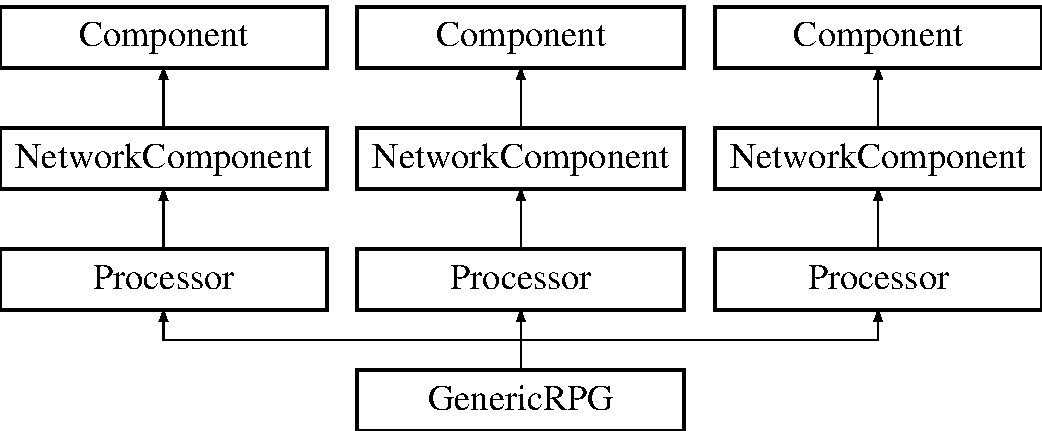
\includegraphics[height=4cm]{classGenericRPG}
\end{center}
\end{figure}
\subsection*{Public Member Functions}
\begin{CompactItemize}
\item 
\hyperlink{classGenericRPG_d909c0fb57cf1b74bacbb0798aa97b29}{GenericRPG} ()
\item 
\hyperlink{classGenericRPG_cff866cbb752b594437b5ddca59e0f03}{$\sim$GenericRPG} ()
\item 
void \hyperlink{classGenericRPG_addf993ae78d1b14589750c78d095aa4}{init\_\-generator} ()
\item 
void \hyperlink{classGenericRPG_e872cb83c70fbf7139fbf1b5cf14310f}{setup} ()
\item 
void \hyperlink{classGenericRPG_03ec120747d2935217291fe23f4c36dd}{finish} ()
\item 
void \hyperlink{classGenericRPG_f6fb1e75e66557481557760c1958612c}{pre\_\-tick} ()
\item 
void \hyperlink{classGenericRPG_f980f5bdb2b703f436b00bb8a318b2fb}{post\_\-tick} ()
\item 
void \hyperlink{classGenericRPG_661b35dacbf7bae62164df5fc1b73477}{idle} ()
\item 
void \hyperlink{classGenericRPG_72d08c87beeb16514c6c81af3296f6af}{process\_\-event} (\hyperlink{classIrisEvent}{IrisEvent} $\ast$e)
\item 
void \hyperlink{classGenericRPG_0f15df71a8cb244d55a2dce961b7a972}{set\_\-no\_\-vcs} (\hyperlink{outputBuffer_8h_91ad9478d81a7aaf2593e8d9c3d06a14}{uint} v)
\item 
string \hyperlink{classGenericRPG_a4303867728559ab6e6ae3d1390ede71}{toString} () const 
\item 
bool \hyperlink{classGenericRPG_4b7a50fa77416fc8b4f16948fb4da592}{compare} ()
\item 
set$<$ \hyperlink{classHighLevelPacket}{HighLevelPacket} $>$ \hyperlink{classGenericRPG_7f855d4d69dc3f019dffdf63d29e2bf4}{get\_\-all\_\-sent} ()
\item 
set$<$ \hyperlink{classHighLevelPacket}{HighLevelPacket} $>$ \hyperlink{classGenericRPG_e6ad83dd5abf9673db6f8bd713979392}{get\_\-all\_\-recv} ()
\item 
void \hyperlink{classGenericRPG_83b1fba5595a25b24b32374ec8e85020}{init} ()
\item 
\hyperlink{classGenericRPG_d909c0fb57cf1b74bacbb0798aa97b29}{GenericRPG} ()
\item 
\hyperlink{classGenericRPG_cff866cbb752b594437b5ddca59e0f03}{$\sim$GenericRPG} ()
\item 
void \hyperlink{classGenericRPG_addf993ae78d1b14589750c78d095aa4}{init\_\-generator} ()
\item 
void \hyperlink{classGenericRPG_e872cb83c70fbf7139fbf1b5cf14310f}{setup} ()
\item 
void \hyperlink{classGenericRPG_03ec120747d2935217291fe23f4c36dd}{finish} ()
\item 
void \hyperlink{classGenericRPG_f6fb1e75e66557481557760c1958612c}{pre\_\-tick} ()
\item 
void \hyperlink{classGenericRPG_f980f5bdb2b703f436b00bb8a318b2fb}{post\_\-tick} ()
\item 
void \hyperlink{classGenericRPG_661b35dacbf7bae62164df5fc1b73477}{idle} ()
\item 
void \hyperlink{classGenericRPG_72d08c87beeb16514c6c81af3296f6af}{process\_\-event} (\hyperlink{classIrisEvent}{IrisEvent} $\ast$e)
\item 
void \hyperlink{classGenericRPG_0f15df71a8cb244d55a2dce961b7a972}{set\_\-no\_\-vcs} (\hyperlink{outputBuffer_8h_91ad9478d81a7aaf2593e8d9c3d06a14}{uint} v)
\item 
string \hyperlink{classGenericRPG_a4303867728559ab6e6ae3d1390ede71}{toString} () const 
\item 
bool \hyperlink{classGenericRPG_4b7a50fa77416fc8b4f16948fb4da592}{compare} ()
\item 
set$<$ \hyperlink{classHighLevelPacket}{HighLevelPacket} $>$ \hyperlink{classGenericRPG_7f855d4d69dc3f019dffdf63d29e2bf4}{get\_\-all\_\-sent} ()
\item 
set$<$ \hyperlink{classHighLevelPacket}{HighLevelPacket} $>$ \hyperlink{classGenericRPG_e6ad83dd5abf9673db6f8bd713979392}{get\_\-all\_\-recv} ()
\item 
void \hyperlink{classGenericRPG_83b1fba5595a25b24b32374ec8e85020}{init} ()
\item 
\hyperlink{classGenericRPG_d909c0fb57cf1b74bacbb0798aa97b29}{GenericRPG} ()
\item 
\hyperlink{classGenericRPG_cff866cbb752b594437b5ddca59e0f03}{$\sim$GenericRPG} ()
\item 
void \hyperlink{classGenericRPG_addf993ae78d1b14589750c78d095aa4}{init\_\-generator} ()
\item 
void \hyperlink{classGenericRPG_e872cb83c70fbf7139fbf1b5cf14310f}{setup} ()
\item 
void \hyperlink{classGenericRPG_03ec120747d2935217291fe23f4c36dd}{finish} ()
\item 
void \hyperlink{classGenericRPG_f6fb1e75e66557481557760c1958612c}{pre\_\-tick} ()
\item 
void \hyperlink{classGenericRPG_f980f5bdb2b703f436b00bb8a318b2fb}{post\_\-tick} ()
\item 
void \hyperlink{classGenericRPG_661b35dacbf7bae62164df5fc1b73477}{idle} ()
\item 
void \hyperlink{classGenericRPG_72d08c87beeb16514c6c81af3296f6af}{process\_\-event} (\hyperlink{classIrisEvent}{IrisEvent} $\ast$e)
\item 
void \hyperlink{classGenericRPG_0f15df71a8cb244d55a2dce961b7a972}{set\_\-no\_\-vcs} (\hyperlink{outputBuffer_8h_91ad9478d81a7aaf2593e8d9c3d06a14}{uint} v)
\item 
string \hyperlink{classGenericRPG_a4303867728559ab6e6ae3d1390ede71}{toString} () const 
\item 
bool \hyperlink{classGenericRPG_4b7a50fa77416fc8b4f16948fb4da592}{compare} ()
\item 
set$<$ \hyperlink{classHighLevelPacket}{HighLevelPacket} $>$ \hyperlink{classGenericRPG_7f855d4d69dc3f019dffdf63d29e2bf4}{get\_\-all\_\-sent} ()
\item 
set$<$ \hyperlink{classHighLevelPacket}{HighLevelPacket} $>$ \hyperlink{classGenericRPG_e6ad83dd5abf9673db6f8bd713979392}{get\_\-all\_\-recv} ()
\item 
void \hyperlink{classGenericRPG_83b1fba5595a25b24b32374ec8e85020}{init} ()
\end{CompactItemize}
\subsection*{Public Attributes}
\begin{CompactItemize}
\item 
unsigned int \hyperlink{classGenericRPG_f0b3d6cc42470254870cd9a919056b05}{packets}
\item 
double \hyperlink{classGenericRPG_408cef6ff9d8c783ca9825101f7a9718}{lamda}
\item 
\hyperlink{classlibRandom_1_1randomNumberGenerator_3bfd56b7b47f4593167e59916a555562}{libRandom::randomNumberGenerator::distribution} \hyperlink{classGenericRPG_1285c700fa0c82d5d79bba983e0fb2c3}{destination\_\-type}
\item 
\hyperlink{classlibRandom_1_1randomNumberGenerator_3bfd56b7b47f4593167e59916a555562}{libRandom::randomNumberGenerator::distribution} \hyperlink{classGenericRPG_db9b1577e85789d95062f9e75d45f183}{length\_\-type}
\item 
\hyperlink{classlibRandom_1_1randomNumberGenerator_3bfd56b7b47f4593167e59916a555562}{libRandom::randomNumberGenerator::distribution} \hyperlink{classGenericRPG_4b27f64374861ba3e2d57451514908f8}{delay\_\-type}
\item 
unsigned int \hyperlink{classGenericRPG_12a401de0099f5d1e2486886d3a99f0f}{address}
\item 
unsigned int \hyperlink{classGenericRPG_ad6fb2a002945d2de4a924bd872031cc}{max\_\-address}
\item 
unsigned int \hyperlink{classGenericRPG_c149370e5d8291090e067e86b1bd5d6d}{min\_\-length}
\item 
unsigned int \hyperlink{classGenericRPG_68d1f82964a4b5c87dd69628912b673f}{max\_\-length}
\item 
unsigned int \hyperlink{classGenericRPG_dbc8b0ba3301646835680aabb98e37bd}{min\_\-delay}
\item 
unsigned int \hyperlink{classGenericRPG_47f854be66ca4cbd5b08aa5c1786bb48}{max\_\-delay}
\item 
unsigned int \hyperlink{classGenericRPG_082010fc167cacf838026859b9b5d3c8}{hot\_\-spots}
\item 
unsigned long long int \hyperlink{classGenericRPG_f306e29286f956ddf0cb021cdd435e93}{max\_\-time}
\item 
unsigned int \hyperlink{classGenericRPG_6a09dde0d73a3d1d89187dc7f0dccc8b}{seed}
\end{CompactItemize}


\subsection{Constructor \& Destructor Documentation}
\hypertarget{classGenericRPG_d909c0fb57cf1b74bacbb0798aa97b29}{
\index{GenericRPG@{GenericRPG}!GenericRPG@{GenericRPG}}
\index{GenericRPG@{GenericRPG}!GenericRPG@{GenericRPG}}
\subsubsection[{GenericRPG}]{\setlength{\rightskip}{0pt plus 5cm}GenericRPG::GenericRPG ()}}
\label{classGenericRPG_d909c0fb57cf1b74bacbb0798aa97b29}


\hypertarget{classGenericRPG_cff866cbb752b594437b5ddca59e0f03}{
\index{GenericRPG@{GenericRPG}!$\sim$GenericRPG@{$\sim$GenericRPG}}
\index{$\sim$GenericRPG@{$\sim$GenericRPG}!GenericRPG@{GenericRPG}}
\subsubsection[{$\sim$GenericRPG}]{\setlength{\rightskip}{0pt plus 5cm}GenericRPG::$\sim$GenericRPG ()}}
\label{classGenericRPG_cff866cbb752b594437b5ddca59e0f03}


\hypertarget{classGenericRPG_d909c0fb57cf1b74bacbb0798aa97b29}{
\index{GenericRPG@{GenericRPG}!GenericRPG@{GenericRPG}}
\index{GenericRPG@{GenericRPG}!GenericRPG@{GenericRPG}}
\subsubsection[{GenericRPG}]{\setlength{\rightskip}{0pt plus 5cm}GenericRPG::GenericRPG ()}}
\label{classGenericRPG_d909c0fb57cf1b74bacbb0798aa97b29}


\hypertarget{classGenericRPG_cff866cbb752b594437b5ddca59e0f03}{
\index{GenericRPG@{GenericRPG}!$\sim$GenericRPG@{$\sim$GenericRPG}}
\index{$\sim$GenericRPG@{$\sim$GenericRPG}!GenericRPG@{GenericRPG}}
\subsubsection[{$\sim$GenericRPG}]{\setlength{\rightskip}{0pt plus 5cm}GenericRPG::$\sim$GenericRPG ()}}
\label{classGenericRPG_cff866cbb752b594437b5ddca59e0f03}


\hypertarget{classGenericRPG_d909c0fb57cf1b74bacbb0798aa97b29}{
\index{GenericRPG@{GenericRPG}!GenericRPG@{GenericRPG}}
\index{GenericRPG@{GenericRPG}!GenericRPG@{GenericRPG}}
\subsubsection[{GenericRPG}]{\setlength{\rightskip}{0pt plus 5cm}GenericRPG::GenericRPG ()}}
\label{classGenericRPG_d909c0fb57cf1b74bacbb0798aa97b29}


\hypertarget{classGenericRPG_cff866cbb752b594437b5ddca59e0f03}{
\index{GenericRPG@{GenericRPG}!$\sim$GenericRPG@{$\sim$GenericRPG}}
\index{$\sim$GenericRPG@{$\sim$GenericRPG}!GenericRPG@{GenericRPG}}
\subsubsection[{$\sim$GenericRPG}]{\setlength{\rightskip}{0pt plus 5cm}GenericRPG::$\sim$GenericRPG ()}}
\label{classGenericRPG_cff866cbb752b594437b5ddca59e0f03}




\subsection{Member Function Documentation}
\hypertarget{classGenericRPG_4b7a50fa77416fc8b4f16948fb4da592}{
\index{GenericRPG@{GenericRPG}!compare@{compare}}
\index{compare@{compare}!GenericRPG@{GenericRPG}}
\subsubsection[{compare}]{\setlength{\rightskip}{0pt plus 5cm}bool GenericRPG::compare ()}}
\label{classGenericRPG_4b7a50fa77416fc8b4f16948fb4da592}


\hypertarget{classGenericRPG_4b7a50fa77416fc8b4f16948fb4da592}{
\index{GenericRPG@{GenericRPG}!compare@{compare}}
\index{compare@{compare}!GenericRPG@{GenericRPG}}
\subsubsection[{compare}]{\setlength{\rightskip}{0pt plus 5cm}bool GenericRPG::compare ()}}
\label{classGenericRPG_4b7a50fa77416fc8b4f16948fb4da592}


\hypertarget{classGenericRPG_4b7a50fa77416fc8b4f16948fb4da592}{
\index{GenericRPG@{GenericRPG}!compare@{compare}}
\index{compare@{compare}!GenericRPG@{GenericRPG}}
\subsubsection[{compare}]{\setlength{\rightskip}{0pt plus 5cm}bool GenericRPG::compare ()}}
\label{classGenericRPG_4b7a50fa77416fc8b4f16948fb4da592}


\hypertarget{classGenericRPG_03ec120747d2935217291fe23f4c36dd}{
\index{GenericRPG@{GenericRPG}!finish@{finish}}
\index{finish@{finish}!GenericRPG@{GenericRPG}}
\subsubsection[{finish}]{\setlength{\rightskip}{0pt plus 5cm}void GenericRPG::finish ()}}
\label{classGenericRPG_03ec120747d2935217291fe23f4c36dd}


\hypertarget{classGenericRPG_03ec120747d2935217291fe23f4c36dd}{
\index{GenericRPG@{GenericRPG}!finish@{finish}}
\index{finish@{finish}!GenericRPG@{GenericRPG}}
\subsubsection[{finish}]{\setlength{\rightskip}{0pt plus 5cm}void GenericRPG::finish ()}}
\label{classGenericRPG_03ec120747d2935217291fe23f4c36dd}


\hypertarget{classGenericRPG_03ec120747d2935217291fe23f4c36dd}{
\index{GenericRPG@{GenericRPG}!finish@{finish}}
\index{finish@{finish}!GenericRPG@{GenericRPG}}
\subsubsection[{finish}]{\setlength{\rightskip}{0pt plus 5cm}void GenericRPG::finish ()}}
\label{classGenericRPG_03ec120747d2935217291fe23f4c36dd}


\hypertarget{classGenericRPG_e6ad83dd5abf9673db6f8bd713979392}{
\index{GenericRPG@{GenericRPG}!get\_\-all\_\-recv@{get\_\-all\_\-recv}}
\index{get\_\-all\_\-recv@{get\_\-all\_\-recv}!GenericRPG@{GenericRPG}}
\subsubsection[{get\_\-all\_\-recv}]{\setlength{\rightskip}{0pt plus 5cm}set$<$ {\bf HighLevelPacket} $>$ GenericRPG::get\_\-all\_\-recv ()}}
\label{classGenericRPG_e6ad83dd5abf9673db6f8bd713979392}


\hypertarget{classGenericRPG_e6ad83dd5abf9673db6f8bd713979392}{
\index{GenericRPG@{GenericRPG}!get\_\-all\_\-recv@{get\_\-all\_\-recv}}
\index{get\_\-all\_\-recv@{get\_\-all\_\-recv}!GenericRPG@{GenericRPG}}
\subsubsection[{get\_\-all\_\-recv}]{\setlength{\rightskip}{0pt plus 5cm}set$<$ {\bf HighLevelPacket} $>$ GenericRPG::get\_\-all\_\-recv ()}}
\label{classGenericRPG_e6ad83dd5abf9673db6f8bd713979392}


\hypertarget{classGenericRPG_e6ad83dd5abf9673db6f8bd713979392}{
\index{GenericRPG@{GenericRPG}!get\_\-all\_\-recv@{get\_\-all\_\-recv}}
\index{get\_\-all\_\-recv@{get\_\-all\_\-recv}!GenericRPG@{GenericRPG}}
\subsubsection[{get\_\-all\_\-recv}]{\setlength{\rightskip}{0pt plus 5cm}set$<$ {\bf HighLevelPacket} $>$ GenericRPG::get\_\-all\_\-recv ()}}
\label{classGenericRPG_e6ad83dd5abf9673db6f8bd713979392}


\hypertarget{classGenericRPG_7f855d4d69dc3f019dffdf63d29e2bf4}{
\index{GenericRPG@{GenericRPG}!get\_\-all\_\-sent@{get\_\-all\_\-sent}}
\index{get\_\-all\_\-sent@{get\_\-all\_\-sent}!GenericRPG@{GenericRPG}}
\subsubsection[{get\_\-all\_\-sent}]{\setlength{\rightskip}{0pt plus 5cm}set$<$ {\bf HighLevelPacket} $>$ GenericRPG::get\_\-all\_\-sent ()}}
\label{classGenericRPG_7f855d4d69dc3f019dffdf63d29e2bf4}


\hypertarget{classGenericRPG_7f855d4d69dc3f019dffdf63d29e2bf4}{
\index{GenericRPG@{GenericRPG}!get\_\-all\_\-sent@{get\_\-all\_\-sent}}
\index{get\_\-all\_\-sent@{get\_\-all\_\-sent}!GenericRPG@{GenericRPG}}
\subsubsection[{get\_\-all\_\-sent}]{\setlength{\rightskip}{0pt plus 5cm}set$<$ {\bf HighLevelPacket} $>$ GenericRPG::get\_\-all\_\-sent ()}}
\label{classGenericRPG_7f855d4d69dc3f019dffdf63d29e2bf4}


\hypertarget{classGenericRPG_7f855d4d69dc3f019dffdf63d29e2bf4}{
\index{GenericRPG@{GenericRPG}!get\_\-all\_\-sent@{get\_\-all\_\-sent}}
\index{get\_\-all\_\-sent@{get\_\-all\_\-sent}!GenericRPG@{GenericRPG}}
\subsubsection[{get\_\-all\_\-sent}]{\setlength{\rightskip}{0pt plus 5cm}set$<$ {\bf HighLevelPacket} $>$ GenericRPG::get\_\-all\_\-sent ()}}
\label{classGenericRPG_7f855d4d69dc3f019dffdf63d29e2bf4}


\hypertarget{classGenericRPG_661b35dacbf7bae62164df5fc1b73477}{
\index{GenericRPG@{GenericRPG}!idle@{idle}}
\index{idle@{idle}!GenericRPG@{GenericRPG}}
\subsubsection[{idle}]{\setlength{\rightskip}{0pt plus 5cm}void GenericRPG::idle ()}}
\label{classGenericRPG_661b35dacbf7bae62164df5fc1b73477}


\hypertarget{classGenericRPG_661b35dacbf7bae62164df5fc1b73477}{
\index{GenericRPG@{GenericRPG}!idle@{idle}}
\index{idle@{idle}!GenericRPG@{GenericRPG}}
\subsubsection[{idle}]{\setlength{\rightskip}{0pt plus 5cm}void GenericRPG::idle ()}}
\label{classGenericRPG_661b35dacbf7bae62164df5fc1b73477}


\hypertarget{classGenericRPG_661b35dacbf7bae62164df5fc1b73477}{
\index{GenericRPG@{GenericRPG}!idle@{idle}}
\index{idle@{idle}!GenericRPG@{GenericRPG}}
\subsubsection[{idle}]{\setlength{\rightskip}{0pt plus 5cm}void GenericRPG::idle ()}}
\label{classGenericRPG_661b35dacbf7bae62164df5fc1b73477}


\hypertarget{classGenericRPG_83b1fba5595a25b24b32374ec8e85020}{
\index{GenericRPG@{GenericRPG}!init@{init}}
\index{init@{init}!GenericRPG@{GenericRPG}}
\subsubsection[{init}]{\setlength{\rightskip}{0pt plus 5cm}void GenericRPG::init ()}}
\label{classGenericRPG_83b1fba5595a25b24b32374ec8e85020}




Reimplemented from \hyperlink{classProcessor_22e869ee49d974ad0ee7ee81961ab88f}{Processor}.\hypertarget{classGenericRPG_83b1fba5595a25b24b32374ec8e85020}{
\index{GenericRPG@{GenericRPG}!init@{init}}
\index{init@{init}!GenericRPG@{GenericRPG}}
\subsubsection[{init}]{\setlength{\rightskip}{0pt plus 5cm}void GenericRPG::init ()}}
\label{classGenericRPG_83b1fba5595a25b24b32374ec8e85020}




Reimplemented from \hyperlink{classProcessor_22e869ee49d974ad0ee7ee81961ab88f}{Processor}.\hypertarget{classGenericRPG_83b1fba5595a25b24b32374ec8e85020}{
\index{GenericRPG@{GenericRPG}!init@{init}}
\index{init@{init}!GenericRPG@{GenericRPG}}
\subsubsection[{init}]{\setlength{\rightskip}{0pt plus 5cm}void GenericRPG::init ()}}
\label{classGenericRPG_83b1fba5595a25b24b32374ec8e85020}




Reimplemented from \hyperlink{classProcessor_22e869ee49d974ad0ee7ee81961ab88f}{Processor}.\hypertarget{classGenericRPG_addf993ae78d1b14589750c78d095aa4}{
\index{GenericRPG@{GenericRPG}!init\_\-generator@{init\_\-generator}}
\index{init\_\-generator@{init\_\-generator}!GenericRPG@{GenericRPG}}
\subsubsection[{init\_\-generator}]{\setlength{\rightskip}{0pt plus 5cm}void GenericRPG::init\_\-generator ()}}
\label{classGenericRPG_addf993ae78d1b14589750c78d095aa4}


\hypertarget{classGenericRPG_addf993ae78d1b14589750c78d095aa4}{
\index{GenericRPG@{GenericRPG}!init\_\-generator@{init\_\-generator}}
\index{init\_\-generator@{init\_\-generator}!GenericRPG@{GenericRPG}}
\subsubsection[{init\_\-generator}]{\setlength{\rightskip}{0pt plus 5cm}void GenericRPG::init\_\-generator ()}}
\label{classGenericRPG_addf993ae78d1b14589750c78d095aa4}


\hypertarget{classGenericRPG_addf993ae78d1b14589750c78d095aa4}{
\index{GenericRPG@{GenericRPG}!init\_\-generator@{init\_\-generator}}
\index{init\_\-generator@{init\_\-generator}!GenericRPG@{GenericRPG}}
\subsubsection[{init\_\-generator}]{\setlength{\rightskip}{0pt plus 5cm}void GenericRPG::init\_\-generator ()}}
\label{classGenericRPG_addf993ae78d1b14589750c78d095aa4}


\hypertarget{classGenericRPG_f980f5bdb2b703f436b00bb8a318b2fb}{
\index{GenericRPG@{GenericRPG}!post\_\-tick@{post\_\-tick}}
\index{post\_\-tick@{post\_\-tick}!GenericRPG@{GenericRPG}}
\subsubsection[{post\_\-tick}]{\setlength{\rightskip}{0pt plus 5cm}void GenericRPG::post\_\-tick ()}}
\label{classGenericRPG_f980f5bdb2b703f436b00bb8a318b2fb}


\hypertarget{classGenericRPG_f980f5bdb2b703f436b00bb8a318b2fb}{
\index{GenericRPG@{GenericRPG}!post\_\-tick@{post\_\-tick}}
\index{post\_\-tick@{post\_\-tick}!GenericRPG@{GenericRPG}}
\subsubsection[{post\_\-tick}]{\setlength{\rightskip}{0pt plus 5cm}void GenericRPG::post\_\-tick ()}}
\label{classGenericRPG_f980f5bdb2b703f436b00bb8a318b2fb}


\hypertarget{classGenericRPG_f980f5bdb2b703f436b00bb8a318b2fb}{
\index{GenericRPG@{GenericRPG}!post\_\-tick@{post\_\-tick}}
\index{post\_\-tick@{post\_\-tick}!GenericRPG@{GenericRPG}}
\subsubsection[{post\_\-tick}]{\setlength{\rightskip}{0pt plus 5cm}void GenericRPG::post\_\-tick ()}}
\label{classGenericRPG_f980f5bdb2b703f436b00bb8a318b2fb}


\hypertarget{classGenericRPG_f6fb1e75e66557481557760c1958612c}{
\index{GenericRPG@{GenericRPG}!pre\_\-tick@{pre\_\-tick}}
\index{pre\_\-tick@{pre\_\-tick}!GenericRPG@{GenericRPG}}
\subsubsection[{pre\_\-tick}]{\setlength{\rightskip}{0pt plus 5cm}void GenericRPG::pre\_\-tick ()}}
\label{classGenericRPG_f6fb1e75e66557481557760c1958612c}


\hypertarget{classGenericRPG_f6fb1e75e66557481557760c1958612c}{
\index{GenericRPG@{GenericRPG}!pre\_\-tick@{pre\_\-tick}}
\index{pre\_\-tick@{pre\_\-tick}!GenericRPG@{GenericRPG}}
\subsubsection[{pre\_\-tick}]{\setlength{\rightskip}{0pt plus 5cm}void GenericRPG::pre\_\-tick ()}}
\label{classGenericRPG_f6fb1e75e66557481557760c1958612c}


\hypertarget{classGenericRPG_f6fb1e75e66557481557760c1958612c}{
\index{GenericRPG@{GenericRPG}!pre\_\-tick@{pre\_\-tick}}
\index{pre\_\-tick@{pre\_\-tick}!GenericRPG@{GenericRPG}}
\subsubsection[{pre\_\-tick}]{\setlength{\rightskip}{0pt plus 5cm}void GenericRPG::pre\_\-tick ()}}
\label{classGenericRPG_f6fb1e75e66557481557760c1958612c}


\hypertarget{classGenericRPG_72d08c87beeb16514c6c81af3296f6af}{
\index{GenericRPG@{GenericRPG}!process\_\-event@{process\_\-event}}
\index{process\_\-event@{process\_\-event}!GenericRPG@{GenericRPG}}
\subsubsection[{process\_\-event}]{\setlength{\rightskip}{0pt plus 5cm}void GenericRPG::process\_\-event ({\bf IrisEvent} $\ast$ {\em e})\hspace{0.3cm}{\tt  \mbox{[}virtual\mbox{]}}}}
\label{classGenericRPG_72d08c87beeb16514c6c81af3296f6af}




Implements \hyperlink{classProcessor_18cdeefafbd8225cb3ad18dd098c0e08}{Processor}.\hypertarget{classGenericRPG_72d08c87beeb16514c6c81af3296f6af}{
\index{GenericRPG@{GenericRPG}!process\_\-event@{process\_\-event}}
\index{process\_\-event@{process\_\-event}!GenericRPG@{GenericRPG}}
\subsubsection[{process\_\-event}]{\setlength{\rightskip}{0pt plus 5cm}void GenericRPG::process\_\-event ({\bf IrisEvent} $\ast$ {\em e})\hspace{0.3cm}{\tt  \mbox{[}virtual\mbox{]}}}}
\label{classGenericRPG_72d08c87beeb16514c6c81af3296f6af}




Implements \hyperlink{classProcessor_18cdeefafbd8225cb3ad18dd098c0e08}{Processor}.\hypertarget{classGenericRPG_72d08c87beeb16514c6c81af3296f6af}{
\index{GenericRPG@{GenericRPG}!process\_\-event@{process\_\-event}}
\index{process\_\-event@{process\_\-event}!GenericRPG@{GenericRPG}}
\subsubsection[{process\_\-event}]{\setlength{\rightskip}{0pt plus 5cm}void GenericRPG::process\_\-event ({\bf IrisEvent} $\ast$ {\em e})\hspace{0.3cm}{\tt  \mbox{[}virtual\mbox{]}}}}
\label{classGenericRPG_72d08c87beeb16514c6c81af3296f6af}




Implements \hyperlink{classProcessor_18cdeefafbd8225cb3ad18dd098c0e08}{Processor}.\hypertarget{classGenericRPG_0f15df71a8cb244d55a2dce961b7a972}{
\index{GenericRPG@{GenericRPG}!set\_\-no\_\-vcs@{set\_\-no\_\-vcs}}
\index{set\_\-no\_\-vcs@{set\_\-no\_\-vcs}!GenericRPG@{GenericRPG}}
\subsubsection[{set\_\-no\_\-vcs}]{\setlength{\rightskip}{0pt plus 5cm}void GenericRPG::set\_\-no\_\-vcs ({\bf uint} {\em v})\hspace{0.3cm}{\tt  \mbox{[}virtual\mbox{]}}}}
\label{classGenericRPG_0f15df71a8cb244d55a2dce961b7a972}




Implements \hyperlink{classProcessor_3280abfe3637712e09cc651b2d09732e}{Processor}.\hypertarget{classGenericRPG_0f15df71a8cb244d55a2dce961b7a972}{
\index{GenericRPG@{GenericRPG}!set\_\-no\_\-vcs@{set\_\-no\_\-vcs}}
\index{set\_\-no\_\-vcs@{set\_\-no\_\-vcs}!GenericRPG@{GenericRPG}}
\subsubsection[{set\_\-no\_\-vcs}]{\setlength{\rightskip}{0pt plus 5cm}void GenericRPG::set\_\-no\_\-vcs ({\bf uint} {\em v})\hspace{0.3cm}{\tt  \mbox{[}virtual\mbox{]}}}}
\label{classGenericRPG_0f15df71a8cb244d55a2dce961b7a972}




Implements \hyperlink{classProcessor_3280abfe3637712e09cc651b2d09732e}{Processor}.\hypertarget{classGenericRPG_0f15df71a8cb244d55a2dce961b7a972}{
\index{GenericRPG@{GenericRPG}!set\_\-no\_\-vcs@{set\_\-no\_\-vcs}}
\index{set\_\-no\_\-vcs@{set\_\-no\_\-vcs}!GenericRPG@{GenericRPG}}
\subsubsection[{set\_\-no\_\-vcs}]{\setlength{\rightskip}{0pt plus 5cm}void GenericRPG::set\_\-no\_\-vcs ({\bf uint} {\em v})\hspace{0.3cm}{\tt  \mbox{[}virtual\mbox{]}}}}
\label{classGenericRPG_0f15df71a8cb244d55a2dce961b7a972}




Implements \hyperlink{classProcessor_3280abfe3637712e09cc651b2d09732e}{Processor}.\hypertarget{classGenericRPG_e872cb83c70fbf7139fbf1b5cf14310f}{
\index{GenericRPG@{GenericRPG}!setup@{setup}}
\index{setup@{setup}!GenericRPG@{GenericRPG}}
\subsubsection[{setup}]{\setlength{\rightskip}{0pt plus 5cm}void GenericRPG::setup ()\hspace{0.3cm}{\tt  \mbox{[}virtual\mbox{]}}}}
\label{classGenericRPG_e872cb83c70fbf7139fbf1b5cf14310f}




Implements \hyperlink{classProcessor_495fad01358e2d9760c526d6e2db53ea}{Processor}.\hypertarget{classGenericRPG_e872cb83c70fbf7139fbf1b5cf14310f}{
\index{GenericRPG@{GenericRPG}!setup@{setup}}
\index{setup@{setup}!GenericRPG@{GenericRPG}}
\subsubsection[{setup}]{\setlength{\rightskip}{0pt plus 5cm}void GenericRPG::setup ()\hspace{0.3cm}{\tt  \mbox{[}virtual\mbox{]}}}}
\label{classGenericRPG_e872cb83c70fbf7139fbf1b5cf14310f}




Implements \hyperlink{classProcessor_495fad01358e2d9760c526d6e2db53ea}{Processor}.\hypertarget{classGenericRPG_e872cb83c70fbf7139fbf1b5cf14310f}{
\index{GenericRPG@{GenericRPG}!setup@{setup}}
\index{setup@{setup}!GenericRPG@{GenericRPG}}
\subsubsection[{setup}]{\setlength{\rightskip}{0pt plus 5cm}void GenericRPG::setup ()\hspace{0.3cm}{\tt  \mbox{[}virtual\mbox{]}}}}
\label{classGenericRPG_e872cb83c70fbf7139fbf1b5cf14310f}




Implements \hyperlink{classProcessor_495fad01358e2d9760c526d6e2db53ea}{Processor}.\hypertarget{classGenericRPG_a4303867728559ab6e6ae3d1390ede71}{
\index{GenericRPG@{GenericRPG}!toString@{toString}}
\index{toString@{toString}!GenericRPG@{GenericRPG}}
\subsubsection[{toString}]{\setlength{\rightskip}{0pt plus 5cm}string GenericRPG::toString () const\hspace{0.3cm}{\tt  \mbox{[}virtual\mbox{]}}}}
\label{classGenericRPG_a4303867728559ab6e6ae3d1390ede71}




Reimplemented from \hyperlink{classProcessor_d3bdbedfbb00b05f61504e411a418106}{Processor}.\hypertarget{classGenericRPG_a4303867728559ab6e6ae3d1390ede71}{
\index{GenericRPG@{GenericRPG}!toString@{toString}}
\index{toString@{toString}!GenericRPG@{GenericRPG}}
\subsubsection[{toString}]{\setlength{\rightskip}{0pt plus 5cm}string GenericRPG::toString () const\hspace{0.3cm}{\tt  \mbox{[}virtual\mbox{]}}}}
\label{classGenericRPG_a4303867728559ab6e6ae3d1390ede71}




Reimplemented from \hyperlink{classProcessor_d3bdbedfbb00b05f61504e411a418106}{Processor}.\hypertarget{classGenericRPG_a4303867728559ab6e6ae3d1390ede71}{
\index{GenericRPG@{GenericRPG}!toString@{toString}}
\index{toString@{toString}!GenericRPG@{GenericRPG}}
\subsubsection[{toString}]{\setlength{\rightskip}{0pt plus 5cm}string GenericRPG::toString () const\hspace{0.3cm}{\tt  \mbox{[}virtual\mbox{]}}}}
\label{classGenericRPG_a4303867728559ab6e6ae3d1390ede71}




Reimplemented from \hyperlink{classProcessor_d3bdbedfbb00b05f61504e411a418106}{Processor}.

\subsection{Member Data Documentation}
\hypertarget{classGenericRPG_12a401de0099f5d1e2486886d3a99f0f}{
\index{GenericRPG@{GenericRPG}!address@{address}}
\index{address@{address}!GenericRPG@{GenericRPG}}
\subsubsection[{address}]{\setlength{\rightskip}{0pt plus 5cm}unsigned int {\bf GenericRPG::address}}}
\label{classGenericRPG_12a401de0099f5d1e2486886d3a99f0f}




Reimplemented from \hyperlink{classNetworkComponent_0428749bde908497630b506071d52191}{NetworkComponent}.\hypertarget{classGenericRPG_4b27f64374861ba3e2d57451514908f8}{
\index{GenericRPG@{GenericRPG}!delay\_\-type@{delay\_\-type}}
\index{delay\_\-type@{delay\_\-type}!GenericRPG@{GenericRPG}}
\subsubsection[{delay\_\-type}]{\setlength{\rightskip}{0pt plus 5cm}{\bf libRandom::randomNumberGenerator::distribution} {\bf GenericRPG::delay\_\-type}}}
\label{classGenericRPG_4b27f64374861ba3e2d57451514908f8}


\hypertarget{classGenericRPG_1285c700fa0c82d5d79bba983e0fb2c3}{
\index{GenericRPG@{GenericRPG}!destination\_\-type@{destination\_\-type}}
\index{destination\_\-type@{destination\_\-type}!GenericRPG@{GenericRPG}}
\subsubsection[{destination\_\-type}]{\setlength{\rightskip}{0pt plus 5cm}{\bf libRandom::randomNumberGenerator::distribution} {\bf GenericRPG::destination\_\-type}}}
\label{classGenericRPG_1285c700fa0c82d5d79bba983e0fb2c3}


\hypertarget{classGenericRPG_082010fc167cacf838026859b9b5d3c8}{
\index{GenericRPG@{GenericRPG}!hot\_\-spots@{hot\_\-spots}}
\index{hot\_\-spots@{hot\_\-spots}!GenericRPG@{GenericRPG}}
\subsubsection[{hot\_\-spots}]{\setlength{\rightskip}{0pt plus 5cm}unsigned int {\bf GenericRPG::hot\_\-spots}}}
\label{classGenericRPG_082010fc167cacf838026859b9b5d3c8}


\hypertarget{classGenericRPG_408cef6ff9d8c783ca9825101f7a9718}{
\index{GenericRPG@{GenericRPG}!lamda@{lamda}}
\index{lamda@{lamda}!GenericRPG@{GenericRPG}}
\subsubsection[{lamda}]{\setlength{\rightskip}{0pt plus 5cm}double {\bf GenericRPG::lamda}}}
\label{classGenericRPG_408cef6ff9d8c783ca9825101f7a9718}


\hypertarget{classGenericRPG_db9b1577e85789d95062f9e75d45f183}{
\index{GenericRPG@{GenericRPG}!length\_\-type@{length\_\-type}}
\index{length\_\-type@{length\_\-type}!GenericRPG@{GenericRPG}}
\subsubsection[{length\_\-type}]{\setlength{\rightskip}{0pt plus 5cm}{\bf libRandom::randomNumberGenerator::distribution} {\bf GenericRPG::length\_\-type}}}
\label{classGenericRPG_db9b1577e85789d95062f9e75d45f183}


\hypertarget{classGenericRPG_ad6fb2a002945d2de4a924bd872031cc}{
\index{GenericRPG@{GenericRPG}!max\_\-address@{max\_\-address}}
\index{max\_\-address@{max\_\-address}!GenericRPG@{GenericRPG}}
\subsubsection[{max\_\-address}]{\setlength{\rightskip}{0pt plus 5cm}unsigned int {\bf GenericRPG::max\_\-address}}}
\label{classGenericRPG_ad6fb2a002945d2de4a924bd872031cc}


\hypertarget{classGenericRPG_47f854be66ca4cbd5b08aa5c1786bb48}{
\index{GenericRPG@{GenericRPG}!max\_\-delay@{max\_\-delay}}
\index{max\_\-delay@{max\_\-delay}!GenericRPG@{GenericRPG}}
\subsubsection[{max\_\-delay}]{\setlength{\rightskip}{0pt plus 5cm}unsigned int {\bf GenericRPG::max\_\-delay}}}
\label{classGenericRPG_47f854be66ca4cbd5b08aa5c1786bb48}


\hypertarget{classGenericRPG_68d1f82964a4b5c87dd69628912b673f}{
\index{GenericRPG@{GenericRPG}!max\_\-length@{max\_\-length}}
\index{max\_\-length@{max\_\-length}!GenericRPG@{GenericRPG}}
\subsubsection[{max\_\-length}]{\setlength{\rightskip}{0pt plus 5cm}unsigned int {\bf GenericRPG::max\_\-length}}}
\label{classGenericRPG_68d1f82964a4b5c87dd69628912b673f}


\hypertarget{classGenericRPG_f306e29286f956ddf0cb021cdd435e93}{
\index{GenericRPG@{GenericRPG}!max\_\-time@{max\_\-time}}
\index{max\_\-time@{max\_\-time}!GenericRPG@{GenericRPG}}
\subsubsection[{max\_\-time}]{\setlength{\rightskip}{0pt plus 5cm}unsigned long long int {\bf GenericRPG::max\_\-time}}}
\label{classGenericRPG_f306e29286f956ddf0cb021cdd435e93}


\hypertarget{classGenericRPG_dbc8b0ba3301646835680aabb98e37bd}{
\index{GenericRPG@{GenericRPG}!min\_\-delay@{min\_\-delay}}
\index{min\_\-delay@{min\_\-delay}!GenericRPG@{GenericRPG}}
\subsubsection[{min\_\-delay}]{\setlength{\rightskip}{0pt plus 5cm}unsigned int {\bf GenericRPG::min\_\-delay}}}
\label{classGenericRPG_dbc8b0ba3301646835680aabb98e37bd}


\hypertarget{classGenericRPG_c149370e5d8291090e067e86b1bd5d6d}{
\index{GenericRPG@{GenericRPG}!min\_\-length@{min\_\-length}}
\index{min\_\-length@{min\_\-length}!GenericRPG@{GenericRPG}}
\subsubsection[{min\_\-length}]{\setlength{\rightskip}{0pt plus 5cm}unsigned int {\bf GenericRPG::min\_\-length}}}
\label{classGenericRPG_c149370e5d8291090e067e86b1bd5d6d}


\hypertarget{classGenericRPG_f0b3d6cc42470254870cd9a919056b05}{
\index{GenericRPG@{GenericRPG}!packets@{packets}}
\index{packets@{packets}!GenericRPG@{GenericRPG}}
\subsubsection[{packets}]{\setlength{\rightskip}{0pt plus 5cm}unsigned int {\bf GenericRPG::packets}}}
\label{classGenericRPG_f0b3d6cc42470254870cd9a919056b05}


\hypertarget{classGenericRPG_6a09dde0d73a3d1d89187dc7f0dccc8b}{
\index{GenericRPG@{GenericRPG}!seed@{seed}}
\index{seed@{seed}!GenericRPG@{GenericRPG}}
\subsubsection[{seed}]{\setlength{\rightskip}{0pt plus 5cm}unsigned int {\bf GenericRPG::seed}}}
\label{classGenericRPG_6a09dde0d73a3d1d89187dc7f0dccc8b}




The documentation for this class was generated from the following files:\begin{CompactItemize}
\item 
source/components/impl/backup/\hyperlink{impl_2backup_2genericRPG_8h}{genericRPG.h}\item 
source/components/impl/\hyperlink{impl_2genericRPG_8h}{genericRPG.h}\item 
source/components/none/\hyperlink{none_2genericRPG_8h}{genericRPG.h}\item 
source/components/impl/backup/\hyperlink{impl_2backup_2genericRPG_8cc}{genericRPG.cc}\item 
source/components/impl/\hyperlink{impl_2genericRPG_8cc}{genericRPG.cc}\item 
source/components/none/\hyperlink{none_2genericRPG_8cc}{genericRPG.cc}\end{CompactItemize}

\hypertarget{classGenericSink}{
\section{GenericSink Class Reference}
\label{classGenericSink}\index{GenericSink@{GenericSink}}
}
{\tt \#include $<$genericSink.h$>$}

Inheritance diagram for GenericSink::\begin{figure}[H]
\begin{center}
\leavevmode
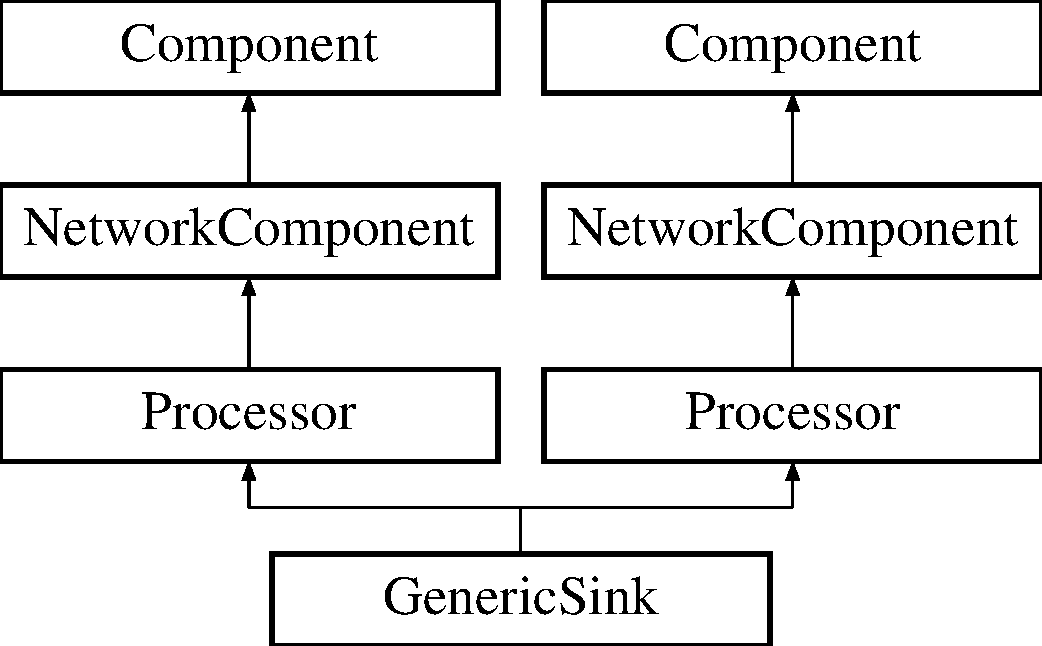
\includegraphics[height=4cm]{classGenericSink}
\end{center}
\end{figure}
\subsection*{Public Member Functions}
\begin{CompactItemize}
\item 
\hyperlink{classGenericSink_6652e97f87a0a6a93dc979a167d2db8b}{GenericSink} ()
\item 
void \hyperlink{classGenericSink_0ed90ea7e6e66cfa8b9935b50ef0051d}{setup} ()
\item 
void \hyperlink{classGenericSink_a0beb58f52adfe869ba47f4b51537409}{process\_\-event} (\hyperlink{classIrisEvent}{IrisEvent} $\ast$e)
\item 
string \hyperlink{classGenericSink_a1703a08208816130a4ee2f4d4a8334f}{toString} () const 
\item 
\hyperlink{classGenericSink_6652e97f87a0a6a93dc979a167d2db8b}{GenericSink} ()
\item 
void \hyperlink{classGenericSink_0ed90ea7e6e66cfa8b9935b50ef0051d}{setup} ()
\item 
void \hyperlink{classGenericSink_a0beb58f52adfe869ba47f4b51537409}{process\_\-event} (\hyperlink{classIrisEvent}{IrisEvent} $\ast$e)
\item 
string \hyperlink{classGenericSink_a1703a08208816130a4ee2f4d4a8334f}{toString} () const 
\end{CompactItemize}
\subsection*{Public Attributes}
\begin{CompactItemize}
\item 
ofstream \hyperlink{classGenericSink_6f54713b76e768ddf16799d4921b497f}{out\_\-file}
\item 
\hyperlink{outputBuffer_8h_91ad9478d81a7aaf2593e8d9c3d06a14}{uint} \hyperlink{classGenericSink_ccb1d47a4bec1322b3e8c996933e4aaf}{address}
\item 
vector$<$ bool $>$ \hyperlink{classGenericSink_ad331b8bfcbeb647f237e5b489868a94}{ready}
\end{CompactItemize}


\subsection{Constructor \& Destructor Documentation}
\hypertarget{classGenericSink_6652e97f87a0a6a93dc979a167d2db8b}{
\index{GenericSink@{GenericSink}!GenericSink@{GenericSink}}
\index{GenericSink@{GenericSink}!GenericSink@{GenericSink}}
\subsubsection[{GenericSink}]{\setlength{\rightskip}{0pt plus 5cm}GenericSink::GenericSink ()}}
\label{classGenericSink_6652e97f87a0a6a93dc979a167d2db8b}


\hypertarget{classGenericSink_6652e97f87a0a6a93dc979a167d2db8b}{
\index{GenericSink@{GenericSink}!GenericSink@{GenericSink}}
\index{GenericSink@{GenericSink}!GenericSink@{GenericSink}}
\subsubsection[{GenericSink}]{\setlength{\rightskip}{0pt plus 5cm}GenericSink::GenericSink ()}}
\label{classGenericSink_6652e97f87a0a6a93dc979a167d2db8b}




\subsection{Member Function Documentation}
\hypertarget{classGenericSink_a0beb58f52adfe869ba47f4b51537409}{
\index{GenericSink@{GenericSink}!process\_\-event@{process\_\-event}}
\index{process\_\-event@{process\_\-event}!GenericSink@{GenericSink}}
\subsubsection[{process\_\-event}]{\setlength{\rightskip}{0pt plus 5cm}void GenericSink::process\_\-event ({\bf IrisEvent} $\ast$ {\em e})\hspace{0.3cm}{\tt  \mbox{[}virtual\mbox{]}}}}
\label{classGenericSink_a0beb58f52adfe869ba47f4b51537409}




Implements \hyperlink{classProcessor_18cdeefafbd8225cb3ad18dd098c0e08}{Processor}.\hypertarget{classGenericSink_a0beb58f52adfe869ba47f4b51537409}{
\index{GenericSink@{GenericSink}!process\_\-event@{process\_\-event}}
\index{process\_\-event@{process\_\-event}!GenericSink@{GenericSink}}
\subsubsection[{process\_\-event}]{\setlength{\rightskip}{0pt plus 5cm}void GenericSink::process\_\-event ({\bf IrisEvent} $\ast$ {\em e})\hspace{0.3cm}{\tt  \mbox{[}virtual\mbox{]}}}}
\label{classGenericSink_a0beb58f52adfe869ba47f4b51537409}




Implements \hyperlink{classProcessor_18cdeefafbd8225cb3ad18dd098c0e08}{Processor}.\hypertarget{classGenericSink_0ed90ea7e6e66cfa8b9935b50ef0051d}{
\index{GenericSink@{GenericSink}!setup@{setup}}
\index{setup@{setup}!GenericSink@{GenericSink}}
\subsubsection[{setup}]{\setlength{\rightskip}{0pt plus 5cm}void GenericSink::setup ()\hspace{0.3cm}{\tt  \mbox{[}virtual\mbox{]}}}}
\label{classGenericSink_0ed90ea7e6e66cfa8b9935b50ef0051d}




Implements \hyperlink{classProcessor_495fad01358e2d9760c526d6e2db53ea}{Processor}.\hypertarget{classGenericSink_0ed90ea7e6e66cfa8b9935b50ef0051d}{
\index{GenericSink@{GenericSink}!setup@{setup}}
\index{setup@{setup}!GenericSink@{GenericSink}}
\subsubsection[{setup}]{\setlength{\rightskip}{0pt plus 5cm}void GenericSink::setup ()\hspace{0.3cm}{\tt  \mbox{[}virtual\mbox{]}}}}
\label{classGenericSink_0ed90ea7e6e66cfa8b9935b50ef0051d}




Implements \hyperlink{classProcessor_495fad01358e2d9760c526d6e2db53ea}{Processor}.\hypertarget{classGenericSink_a1703a08208816130a4ee2f4d4a8334f}{
\index{GenericSink@{GenericSink}!toString@{toString}}
\index{toString@{toString}!GenericSink@{GenericSink}}
\subsubsection[{toString}]{\setlength{\rightskip}{0pt plus 5cm}string GenericSink::toString () const\hspace{0.3cm}{\tt  \mbox{[}virtual\mbox{]}}}}
\label{classGenericSink_a1703a08208816130a4ee2f4d4a8334f}




Reimplemented from \hyperlink{classProcessor_d3bdbedfbb00b05f61504e411a418106}{Processor}.\hypertarget{classGenericSink_a1703a08208816130a4ee2f4d4a8334f}{
\index{GenericSink@{GenericSink}!toString@{toString}}
\index{toString@{toString}!GenericSink@{GenericSink}}
\subsubsection[{toString}]{\setlength{\rightskip}{0pt plus 5cm}string GenericSink::toString () const\hspace{0.3cm}{\tt  \mbox{[}virtual\mbox{]}}}}
\label{classGenericSink_a1703a08208816130a4ee2f4d4a8334f}




Reimplemented from \hyperlink{classProcessor_d3bdbedfbb00b05f61504e411a418106}{Processor}.

\subsection{Member Data Documentation}
\hypertarget{classGenericSink_ccb1d47a4bec1322b3e8c996933e4aaf}{
\index{GenericSink@{GenericSink}!address@{address}}
\index{address@{address}!GenericSink@{GenericSink}}
\subsubsection[{address}]{\setlength{\rightskip}{0pt plus 5cm}{\bf uint} {\bf GenericSink::address}}}
\label{classGenericSink_ccb1d47a4bec1322b3e8c996933e4aaf}




Reimplemented from \hyperlink{classNetworkComponent_0428749bde908497630b506071d52191}{NetworkComponent}.\hypertarget{classGenericSink_6f54713b76e768ddf16799d4921b497f}{
\index{GenericSink@{GenericSink}!out\_\-file@{out\_\-file}}
\index{out\_\-file@{out\_\-file}!GenericSink@{GenericSink}}
\subsubsection[{out\_\-file}]{\setlength{\rightskip}{0pt plus 5cm}ofstream {\bf GenericSink::out\_\-file}}}
\label{classGenericSink_6f54713b76e768ddf16799d4921b497f}


\hypertarget{classGenericSink_ad331b8bfcbeb647f237e5b489868a94}{
\index{GenericSink@{GenericSink}!ready@{ready}}
\index{ready@{ready}!GenericSink@{GenericSink}}
\subsubsection[{ready}]{\setlength{\rightskip}{0pt plus 5cm}vector$<$ bool $>$ {\bf GenericSink::ready}}}
\label{classGenericSink_ad331b8bfcbeb647f237e5b489868a94}




The documentation for this class was generated from the following files:\begin{CompactItemize}
\item 
source/components/impl/\hyperlink{impl_2genericSink_8h}{genericSink.h}\item 
source/components/none/\hyperlink{none_2genericSink_8h}{genericSink.h}\item 
source/components/impl/\hyperlink{impl_2genericSink_8cc}{genericSink.cc}\item 
source/components/none/\hyperlink{none_2genericSink_8cc}{genericSink.cc}\end{CompactItemize}

\hypertarget{classGenericTPG}{
\section{GenericTPG Class Reference}
\label{classGenericTPG}\index{GenericTPG@{GenericTPG}}
}
{\tt \#include $<$genericTPG.h$>$}

Inheritance diagram for GenericTPG::\begin{figure}[H]
\begin{center}
\leavevmode
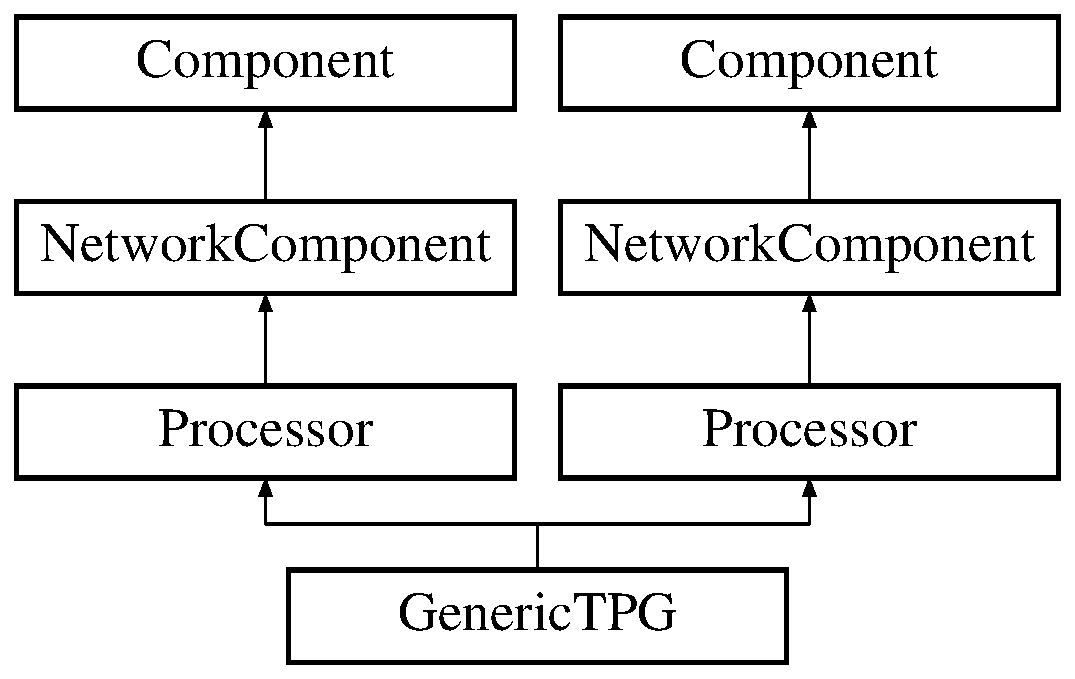
\includegraphics[height=4cm]{classGenericTPG}
\end{center}
\end{figure}
\subsection*{Public Member Functions}
\begin{CompactItemize}
\item 
\hyperlink{classGenericTPG_4caf5cdc5c95a600391ecd2eb2c071fc}{GenericTPG} ()
\item 
\hyperlink{classGenericTPG_f1c645245af41d6b21eef232ff65587a}{$\sim$GenericTPG} ()
\item 
void \hyperlink{classGenericTPG_5cea355b4db26ed22a7af8e54758de47}{setup} ()
\item 
void \hyperlink{classGenericTPG_8dd8fa2cd2721789a63084d8fe912366}{finish} ()
\item 
void \hyperlink{classGenericTPG_a2e59f102384206268808835bcb9d5b5}{process\_\-event} (\hyperlink{classIrisEvent}{IrisEvent} $\ast$e)
\item 
string \hyperlink{classGenericTPG_c2e1dc7b0de824c846f37c4a1c282303}{toString} () const 
\item 
void \hyperlink{classGenericTPG_fe1f30bce868ee2caa01d3f7a2229945}{set\_\-trace\_\-filename} (string filename)
\item 
void \hyperlink{classGenericTPG_e95391a655cacb75ba23e7eb8b3cefef}{set\_\-no\_\-vcs} (\hyperlink{outputBuffer_8h_91ad9478d81a7aaf2593e8d9c3d06a14}{uint} v)
\item 
bool \hyperlink{classGenericTPG_d26b3d9a264ebe07d44b9194626c98d7}{compare} ()
\item 
set$<$ \hyperlink{classHighLevelPacket}{HighLevelPacket} $>$ \hyperlink{classGenericTPG_2b424dd4b2f5aa07a0231d69d5790470}{get\_\-all\_\-sent} ()
\item 
set$<$ \hyperlink{classHighLevelPacket}{HighLevelPacket} $>$ \hyperlink{classGenericTPG_aca7529b0e19d664ee40392b7761e338}{get\_\-all\_\-recv} ()
\item 
bool \hyperlink{classGenericTPG_e0d0461b59107eb3b4facb4d29ada948}{GetNewRequest} (\hyperlink{classRequest}{Request} $\ast$req)
\item 
\hyperlink{classRequest}{Request} $\ast$ \hyperlink{classGenericTPG_ec1a1105fdd72ac3ba86ab577c1f5226}{GetRequest} ()
\item 
\hyperlink{classGenericTPG_4caf5cdc5c95a600391ecd2eb2c071fc}{GenericTPG} ()
\item 
\hyperlink{classGenericTPG_f1c645245af41d6b21eef232ff65587a}{$\sim$GenericTPG} ()
\item 
void \hyperlink{classGenericTPG_5cea355b4db26ed22a7af8e54758de47}{setup} ()
\item 
void \hyperlink{classGenericTPG_8dd8fa2cd2721789a63084d8fe912366}{finish} ()
\item 
void \hyperlink{classGenericTPG_a2e59f102384206268808835bcb9d5b5}{process\_\-event} (\hyperlink{classIrisEvent}{IrisEvent} $\ast$e)
\item 
string \hyperlink{classGenericTPG_c2e1dc7b0de824c846f37c4a1c282303}{toString} () const 
\item 
void \hyperlink{classGenericTPG_fe1f30bce868ee2caa01d3f7a2229945}{set\_\-trace\_\-filename} (string filename)
\item 
void \hyperlink{classGenericTPG_e95391a655cacb75ba23e7eb8b3cefef}{set\_\-no\_\-vcs} (\hyperlink{outputBuffer_8h_91ad9478d81a7aaf2593e8d9c3d06a14}{uint} v)
\item 
bool \hyperlink{classGenericTPG_d26b3d9a264ebe07d44b9194626c98d7}{compare} ()
\item 
set$<$ \hyperlink{classHighLevelPacket}{HighLevelPacket} $>$ \hyperlink{classGenericTPG_2b424dd4b2f5aa07a0231d69d5790470}{get\_\-all\_\-sent} ()
\item 
set$<$ \hyperlink{classHighLevelPacket}{HighLevelPacket} $>$ \hyperlink{classGenericTPG_aca7529b0e19d664ee40392b7761e338}{get\_\-all\_\-recv} ()
\item 
bool \hyperlink{classGenericTPG_e0d0461b59107eb3b4facb4d29ada948}{GetNewRequest} (\hyperlink{classRequest}{Request} $\ast$req)
\item 
\hyperlink{classRequest}{Request} $\ast$ \hyperlink{classGenericTPG_2e30905e10685209af2c6ff15bb4f07a}{GetRequest} ()
\end{CompactItemize}
\subsection*{Public Attributes}
\begin{CompactItemize}
\item 
unsigned int \hyperlink{classGenericTPG_373e1e2904c42be961f521c8b32e9f1e}{packets}
\item 
\hyperlink{classMSHR__H}{MSHR\_\-H} $\ast$ \hyperlink{classGenericTPG_03a0346d54282502eae314c9525da513}{mshrHandler}
\item 
unsigned long long int \hyperlink{classGenericTPG_f2b6690d9c38e72a408cde91480fe13e}{max\_\-time}
\end{CompactItemize}


\subsection{Constructor \& Destructor Documentation}
\hypertarget{classGenericTPG_4caf5cdc5c95a600391ecd2eb2c071fc}{
\index{GenericTPG@{GenericTPG}!GenericTPG@{GenericTPG}}
\index{GenericTPG@{GenericTPG}!GenericTPG@{GenericTPG}}
\subsubsection[{GenericTPG}]{\setlength{\rightskip}{0pt plus 5cm}GenericTPG::GenericTPG ()}}
\label{classGenericTPG_4caf5cdc5c95a600391ecd2eb2c071fc}


\hypertarget{classGenericTPG_f1c645245af41d6b21eef232ff65587a}{
\index{GenericTPG@{GenericTPG}!$\sim$GenericTPG@{$\sim$GenericTPG}}
\index{$\sim$GenericTPG@{$\sim$GenericTPG}!GenericTPG@{GenericTPG}}
\subsubsection[{$\sim$GenericTPG}]{\setlength{\rightskip}{0pt plus 5cm}GenericTPG::$\sim$GenericTPG ()}}
\label{classGenericTPG_f1c645245af41d6b21eef232ff65587a}


\hypertarget{classGenericTPG_4caf5cdc5c95a600391ecd2eb2c071fc}{
\index{GenericTPG@{GenericTPG}!GenericTPG@{GenericTPG}}
\index{GenericTPG@{GenericTPG}!GenericTPG@{GenericTPG}}
\subsubsection[{GenericTPG}]{\setlength{\rightskip}{0pt plus 5cm}GenericTPG::GenericTPG ()}}
\label{classGenericTPG_4caf5cdc5c95a600391ecd2eb2c071fc}


\hypertarget{classGenericTPG_f1c645245af41d6b21eef232ff65587a}{
\index{GenericTPG@{GenericTPG}!$\sim$GenericTPG@{$\sim$GenericTPG}}
\index{$\sim$GenericTPG@{$\sim$GenericTPG}!GenericTPG@{GenericTPG}}
\subsubsection[{$\sim$GenericTPG}]{\setlength{\rightskip}{0pt plus 5cm}GenericTPG::$\sim$GenericTPG ()}}
\label{classGenericTPG_f1c645245af41d6b21eef232ff65587a}




\subsection{Member Function Documentation}
\hypertarget{classGenericTPG_d26b3d9a264ebe07d44b9194626c98d7}{
\index{GenericTPG@{GenericTPG}!compare@{compare}}
\index{compare@{compare}!GenericTPG@{GenericTPG}}
\subsubsection[{compare}]{\setlength{\rightskip}{0pt plus 5cm}bool GenericTPG::compare ()}}
\label{classGenericTPG_d26b3d9a264ebe07d44b9194626c98d7}


\hypertarget{classGenericTPG_d26b3d9a264ebe07d44b9194626c98d7}{
\index{GenericTPG@{GenericTPG}!compare@{compare}}
\index{compare@{compare}!GenericTPG@{GenericTPG}}
\subsubsection[{compare}]{\setlength{\rightskip}{0pt plus 5cm}bool GenericTPG::compare ()}}
\label{classGenericTPG_d26b3d9a264ebe07d44b9194626c98d7}


\hypertarget{classGenericTPG_8dd8fa2cd2721789a63084d8fe912366}{
\index{GenericTPG@{GenericTPG}!finish@{finish}}
\index{finish@{finish}!GenericTPG@{GenericTPG}}
\subsubsection[{finish}]{\setlength{\rightskip}{0pt plus 5cm}void GenericTPG::finish ()}}
\label{classGenericTPG_8dd8fa2cd2721789a63084d8fe912366}


\hypertarget{classGenericTPG_8dd8fa2cd2721789a63084d8fe912366}{
\index{GenericTPG@{GenericTPG}!finish@{finish}}
\index{finish@{finish}!GenericTPG@{GenericTPG}}
\subsubsection[{finish}]{\setlength{\rightskip}{0pt plus 5cm}void GenericTPG::finish ()}}
\label{classGenericTPG_8dd8fa2cd2721789a63084d8fe912366}


\hypertarget{classGenericTPG_aca7529b0e19d664ee40392b7761e338}{
\index{GenericTPG@{GenericTPG}!get\_\-all\_\-recv@{get\_\-all\_\-recv}}
\index{get\_\-all\_\-recv@{get\_\-all\_\-recv}!GenericTPG@{GenericTPG}}
\subsubsection[{get\_\-all\_\-recv}]{\setlength{\rightskip}{0pt plus 5cm}set$<$ {\bf HighLevelPacket} $>$ GenericTPG::get\_\-all\_\-recv ()}}
\label{classGenericTPG_aca7529b0e19d664ee40392b7761e338}


\hypertarget{classGenericTPG_aca7529b0e19d664ee40392b7761e338}{
\index{GenericTPG@{GenericTPG}!get\_\-all\_\-recv@{get\_\-all\_\-recv}}
\index{get\_\-all\_\-recv@{get\_\-all\_\-recv}!GenericTPG@{GenericTPG}}
\subsubsection[{get\_\-all\_\-recv}]{\setlength{\rightskip}{0pt plus 5cm}set$<$ {\bf HighLevelPacket} $>$ GenericTPG::get\_\-all\_\-recv ()}}
\label{classGenericTPG_aca7529b0e19d664ee40392b7761e338}


\hypertarget{classGenericTPG_2b424dd4b2f5aa07a0231d69d5790470}{
\index{GenericTPG@{GenericTPG}!get\_\-all\_\-sent@{get\_\-all\_\-sent}}
\index{get\_\-all\_\-sent@{get\_\-all\_\-sent}!GenericTPG@{GenericTPG}}
\subsubsection[{get\_\-all\_\-sent}]{\setlength{\rightskip}{0pt plus 5cm}set$<$ {\bf HighLevelPacket} $>$ GenericTPG::get\_\-all\_\-sent ()}}
\label{classGenericTPG_2b424dd4b2f5aa07a0231d69d5790470}


\hypertarget{classGenericTPG_2b424dd4b2f5aa07a0231d69d5790470}{
\index{GenericTPG@{GenericTPG}!get\_\-all\_\-sent@{get\_\-all\_\-sent}}
\index{get\_\-all\_\-sent@{get\_\-all\_\-sent}!GenericTPG@{GenericTPG}}
\subsubsection[{get\_\-all\_\-sent}]{\setlength{\rightskip}{0pt plus 5cm}set$<$ {\bf HighLevelPacket} $>$ GenericTPG::get\_\-all\_\-sent ()}}
\label{classGenericTPG_2b424dd4b2f5aa07a0231d69d5790470}


\hypertarget{classGenericTPG_e0d0461b59107eb3b4facb4d29ada948}{
\index{GenericTPG@{GenericTPG}!GetNewRequest@{GetNewRequest}}
\index{GetNewRequest@{GetNewRequest}!GenericTPG@{GenericTPG}}
\subsubsection[{GetNewRequest}]{\setlength{\rightskip}{0pt plus 5cm}bool GenericTPG::GetNewRequest ({\bf Request} $\ast$ {\em req})}}
\label{classGenericTPG_e0d0461b59107eb3b4facb4d29ada948}


\hypertarget{classGenericTPG_e0d0461b59107eb3b4facb4d29ada948}{
\index{GenericTPG@{GenericTPG}!GetNewRequest@{GetNewRequest}}
\index{GetNewRequest@{GetNewRequest}!GenericTPG@{GenericTPG}}
\subsubsection[{GetNewRequest}]{\setlength{\rightskip}{0pt plus 5cm}bool GenericTPG::GetNewRequest ({\bf Request} $\ast$ {\em req})}}
\label{classGenericTPG_e0d0461b59107eb3b4facb4d29ada948}


\hypertarget{classGenericTPG_2e30905e10685209af2c6ff15bb4f07a}{
\index{GenericTPG@{GenericTPG}!GetRequest@{GetRequest}}
\index{GetRequest@{GetRequest}!GenericTPG@{GenericTPG}}
\subsubsection[{GetRequest}]{\setlength{\rightskip}{0pt plus 5cm}{\bf Request}$\ast$ GenericTPG::GetRequest ()}}
\label{classGenericTPG_2e30905e10685209af2c6ff15bb4f07a}


\hypertarget{classGenericTPG_ec1a1105fdd72ac3ba86ab577c1f5226}{
\index{GenericTPG@{GenericTPG}!GetRequest@{GetRequest}}
\index{GetRequest@{GetRequest}!GenericTPG@{GenericTPG}}
\subsubsection[{GetRequest}]{\setlength{\rightskip}{0pt plus 5cm}{\bf Request} $\ast$ GenericTPG::GetRequest ()}}
\label{classGenericTPG_ec1a1105fdd72ac3ba86ab577c1f5226}


\hypertarget{classGenericTPG_a2e59f102384206268808835bcb9d5b5}{
\index{GenericTPG@{GenericTPG}!process\_\-event@{process\_\-event}}
\index{process\_\-event@{process\_\-event}!GenericTPG@{GenericTPG}}
\subsubsection[{process\_\-event}]{\setlength{\rightskip}{0pt plus 5cm}void GenericTPG::process\_\-event ({\bf IrisEvent} $\ast$ {\em e})\hspace{0.3cm}{\tt  \mbox{[}virtual\mbox{]}}}}
\label{classGenericTPG_a2e59f102384206268808835bcb9d5b5}




Implements \hyperlink{classProcessor_18cdeefafbd8225cb3ad18dd098c0e08}{Processor}.\hypertarget{classGenericTPG_a2e59f102384206268808835bcb9d5b5}{
\index{GenericTPG@{GenericTPG}!process\_\-event@{process\_\-event}}
\index{process\_\-event@{process\_\-event}!GenericTPG@{GenericTPG}}
\subsubsection[{process\_\-event}]{\setlength{\rightskip}{0pt plus 5cm}void GenericTPG::process\_\-event ({\bf IrisEvent} $\ast$ {\em e})\hspace{0.3cm}{\tt  \mbox{[}virtual\mbox{]}}}}
\label{classGenericTPG_a2e59f102384206268808835bcb9d5b5}




Implements \hyperlink{classProcessor_18cdeefafbd8225cb3ad18dd098c0e08}{Processor}.\hypertarget{classGenericTPG_e95391a655cacb75ba23e7eb8b3cefef}{
\index{GenericTPG@{GenericTPG}!set\_\-no\_\-vcs@{set\_\-no\_\-vcs}}
\index{set\_\-no\_\-vcs@{set\_\-no\_\-vcs}!GenericTPG@{GenericTPG}}
\subsubsection[{set\_\-no\_\-vcs}]{\setlength{\rightskip}{0pt plus 5cm}void GenericTPG::set\_\-no\_\-vcs ({\bf uint} {\em v})\hspace{0.3cm}{\tt  \mbox{[}virtual\mbox{]}}}}
\label{classGenericTPG_e95391a655cacb75ba23e7eb8b3cefef}




Implements \hyperlink{classProcessor_3280abfe3637712e09cc651b2d09732e}{Processor}.\hypertarget{classGenericTPG_e95391a655cacb75ba23e7eb8b3cefef}{
\index{GenericTPG@{GenericTPG}!set\_\-no\_\-vcs@{set\_\-no\_\-vcs}}
\index{set\_\-no\_\-vcs@{set\_\-no\_\-vcs}!GenericTPG@{GenericTPG}}
\subsubsection[{set\_\-no\_\-vcs}]{\setlength{\rightskip}{0pt plus 5cm}void GenericTPG::set\_\-no\_\-vcs ({\bf uint} {\em v})\hspace{0.3cm}{\tt  \mbox{[}virtual\mbox{]}}}}
\label{classGenericTPG_e95391a655cacb75ba23e7eb8b3cefef}




Implements \hyperlink{classProcessor_3280abfe3637712e09cc651b2d09732e}{Processor}.\hypertarget{classGenericTPG_fe1f30bce868ee2caa01d3f7a2229945}{
\index{GenericTPG@{GenericTPG}!set\_\-trace\_\-filename@{set\_\-trace\_\-filename}}
\index{set\_\-trace\_\-filename@{set\_\-trace\_\-filename}!GenericTPG@{GenericTPG}}
\subsubsection[{set\_\-trace\_\-filename}]{\setlength{\rightskip}{0pt plus 5cm}void GenericTPG::set\_\-trace\_\-filename (string {\em filename})}}
\label{classGenericTPG_fe1f30bce868ee2caa01d3f7a2229945}


\hypertarget{classGenericTPG_fe1f30bce868ee2caa01d3f7a2229945}{
\index{GenericTPG@{GenericTPG}!set\_\-trace\_\-filename@{set\_\-trace\_\-filename}}
\index{set\_\-trace\_\-filename@{set\_\-trace\_\-filename}!GenericTPG@{GenericTPG}}
\subsubsection[{set\_\-trace\_\-filename}]{\setlength{\rightskip}{0pt plus 5cm}void GenericTPG::set\_\-trace\_\-filename (string {\em filename})}}
\label{classGenericTPG_fe1f30bce868ee2caa01d3f7a2229945}


\hypertarget{classGenericTPG_5cea355b4db26ed22a7af8e54758de47}{
\index{GenericTPG@{GenericTPG}!setup@{setup}}
\index{setup@{setup}!GenericTPG@{GenericTPG}}
\subsubsection[{setup}]{\setlength{\rightskip}{0pt plus 5cm}void GenericTPG::setup ()\hspace{0.3cm}{\tt  \mbox{[}virtual\mbox{]}}}}
\label{classGenericTPG_5cea355b4db26ed22a7af8e54758de47}




Implements \hyperlink{classProcessor_495fad01358e2d9760c526d6e2db53ea}{Processor}.\hypertarget{classGenericTPG_5cea355b4db26ed22a7af8e54758de47}{
\index{GenericTPG@{GenericTPG}!setup@{setup}}
\index{setup@{setup}!GenericTPG@{GenericTPG}}
\subsubsection[{setup}]{\setlength{\rightskip}{0pt plus 5cm}void GenericTPG::setup ()\hspace{0.3cm}{\tt  \mbox{[}virtual\mbox{]}}}}
\label{classGenericTPG_5cea355b4db26ed22a7af8e54758de47}




Implements \hyperlink{classProcessor_495fad01358e2d9760c526d6e2db53ea}{Processor}.\hypertarget{classGenericTPG_c2e1dc7b0de824c846f37c4a1c282303}{
\index{GenericTPG@{GenericTPG}!toString@{toString}}
\index{toString@{toString}!GenericTPG@{GenericTPG}}
\subsubsection[{toString}]{\setlength{\rightskip}{0pt plus 5cm}string GenericTPG::toString () const\hspace{0.3cm}{\tt  \mbox{[}virtual\mbox{]}}}}
\label{classGenericTPG_c2e1dc7b0de824c846f37c4a1c282303}




Reimplemented from \hyperlink{classProcessor_d3bdbedfbb00b05f61504e411a418106}{Processor}.\hypertarget{classGenericTPG_c2e1dc7b0de824c846f37c4a1c282303}{
\index{GenericTPG@{GenericTPG}!toString@{toString}}
\index{toString@{toString}!GenericTPG@{GenericTPG}}
\subsubsection[{toString}]{\setlength{\rightskip}{0pt plus 5cm}string GenericTPG::toString () const\hspace{0.3cm}{\tt  \mbox{[}virtual\mbox{]}}}}
\label{classGenericTPG_c2e1dc7b0de824c846f37c4a1c282303}




Reimplemented from \hyperlink{classProcessor_d3bdbedfbb00b05f61504e411a418106}{Processor}.

\subsection{Member Data Documentation}
\hypertarget{classGenericTPG_f2b6690d9c38e72a408cde91480fe13e}{
\index{GenericTPG@{GenericTPG}!max\_\-time@{max\_\-time}}
\index{max\_\-time@{max\_\-time}!GenericTPG@{GenericTPG}}
\subsubsection[{max\_\-time}]{\setlength{\rightskip}{0pt plus 5cm}unsigned long long int {\bf GenericTPG::max\_\-time}}}
\label{classGenericTPG_f2b6690d9c38e72a408cde91480fe13e}


\hypertarget{classGenericTPG_03a0346d54282502eae314c9525da513}{
\index{GenericTPG@{GenericTPG}!mshrHandler@{mshrHandler}}
\index{mshrHandler@{mshrHandler}!GenericTPG@{GenericTPG}}
\subsubsection[{mshrHandler}]{\setlength{\rightskip}{0pt plus 5cm}{\bf MSHR\_\-H} $\ast$ {\bf GenericTPG::mshrHandler}}}
\label{classGenericTPG_03a0346d54282502eae314c9525da513}


\hypertarget{classGenericTPG_373e1e2904c42be961f521c8b32e9f1e}{
\index{GenericTPG@{GenericTPG}!packets@{packets}}
\index{packets@{packets}!GenericTPG@{GenericTPG}}
\subsubsection[{packets}]{\setlength{\rightskip}{0pt plus 5cm}unsigned int {\bf GenericTPG::packets}}}
\label{classGenericTPG_373e1e2904c42be961f521c8b32e9f1e}




The documentation for this class was generated from the following files:\begin{CompactItemize}
\item 
source/components/impl/\hyperlink{impl_2genericTPG_8h}{genericTPG.h}\item 
source/components/none/\hyperlink{none_2genericTPG_8h}{genericTPG.h}\item 
source/components/impl/\hyperlink{impl_2genericTPG_8cc}{genericTPG.cc}\item 
source/components/impl/\hyperlink{impl_2genericTPG__temp_8cc}{genericTPG\_\-temp.cc}\item 
source/components/none/\hyperlink{none_2genericTPG_8cc}{genericTPG.cc}\item 
source/components/none/\hyperlink{none_2genericTPG__temp_8cc}{genericTPG\_\-temp.cc}\end{CompactItemize}

\hypertarget{classGenericVcArbiter}{
\section{GenericVcArbiter Class Reference}
\label{classGenericVcArbiter}\index{GenericVcArbiter@{GenericVcArbiter}}
}
{\tt \#include $<$genericVcArbiter.h$>$}

Inheritance diagram for GenericVcArbiter::\begin{figure}[H]
\begin{center}
\leavevmode
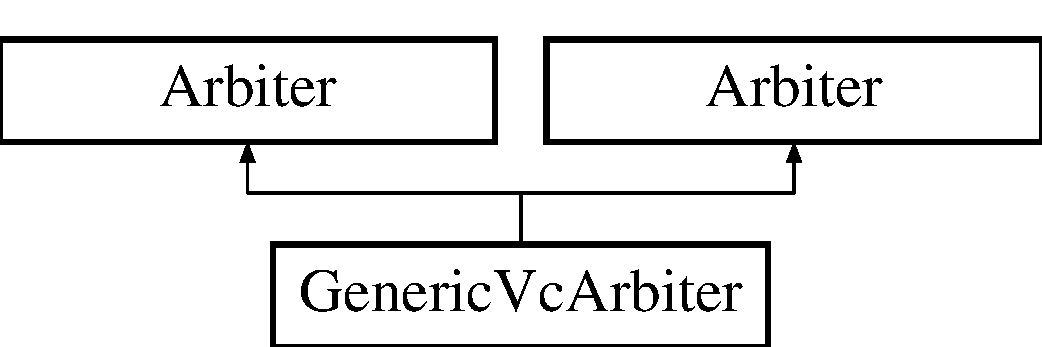
\includegraphics[height=2cm]{classGenericVcArbiter}
\end{center}
\end{figure}
\subsection*{Public Member Functions}
\begin{CompactItemize}
\item 
\hyperlink{classGenericVcArbiter_8ad20b81e2a38303b310d15e1dcc9947}{GenericVcArbiter} ()
\item 
\hyperlink{classGenericVcArbiter_da76ff9f227949f97ecd02d1bf89b5c8}{$\sim$GenericVcArbiter} ()
\item 
bool \hyperlink{classGenericVcArbiter_bea0f63a51a1bfbfe7bd3a3ee0b95b48}{is\_\-requested} (\hyperlink{outputBuffer_8h_91ad9478d81a7aaf2593e8d9c3d06a14}{uint} ch)
\item 
void \hyperlink{classGenericVcArbiter_9424efde9588993e6b7315bd8e536ee9}{set\_\-req\_\-queue\_\-size} (\hyperlink{outputBuffer_8h_91ad9478d81a7aaf2593e8d9c3d06a14}{uint} size)
\item 
void \hyperlink{classGenericVcArbiter_c118c1a5cc6a9d105cd6ac5c54c7fe77}{request} (\hyperlink{classFlit}{Flit} $\ast$f, \hyperlink{outputBuffer_8h_91ad9478d81a7aaf2593e8d9c3d06a14}{uint} index)
\item 
\hyperlink{classFlit}{Flit} $\ast$ \hyperlink{classGenericVcArbiter_af615d6c6a206070c87e2ecdf82a717d}{pull\_\-winner} ()
\item 
\hyperlink{outputBuffer_8h_91ad9478d81a7aaf2593e8d9c3d06a14}{uint} \hyperlink{classGenericVcArbiter_0648f3756140fa6acc1e9345015b3461}{get\_\-no\_\-requests} ()
\item 
\hyperlink{outputBuffer_8h_91ad9478d81a7aaf2593e8d9c3d06a14}{uint} \hyperlink{classGenericVcArbiter_55ce40bdf8fa7c2ea448ee5aa5c50921}{pick\_\-winner} ()
\item 
\hyperlink{outputBuffer_8h_91ad9478d81a7aaf2593e8d9c3d06a14}{uint} \hyperlink{classGenericVcArbiter_d5d1e1d3532c52f4e3cdb92ab2a235ec}{pick\_\-winner} (vector$<$ bool $>$ ready)
\item 
void \hyperlink{classGenericVcArbiter_4cd15ea7b1b8ff50cbd9148826880fdf}{clear\_\-winner} ()
\item 
bool \hyperlink{classGenericVcArbiter_c03a3978b5564acfd561a097384570d5}{empty} ()
\item 
bool \hyperlink{classGenericVcArbiter_89fe4818dbc079a5305db9cfe23fd5a3}{empty} (vector$<$ bool $>$ ready)
\item 
string \hyperlink{classGenericVcArbiter_b2b98c13d7e7c13e703845591f241e70}{toString} () const 
\item 
\hyperlink{classGenericVcArbiter_8ad20b81e2a38303b310d15e1dcc9947}{GenericVcArbiter} ()
\item 
\hyperlink{classGenericVcArbiter_da76ff9f227949f97ecd02d1bf89b5c8}{$\sim$GenericVcArbiter} ()
\item 
bool \hyperlink{classGenericVcArbiter_bea0f63a51a1bfbfe7bd3a3ee0b95b48}{is\_\-requested} (\hyperlink{outputBuffer_8h_91ad9478d81a7aaf2593e8d9c3d06a14}{uint} ch)
\item 
void \hyperlink{classGenericVcArbiter_ec3307aa2de2dd6c8776102a950a4783}{set\_\-no\_\-vcs} (\hyperlink{outputBuffer_8h_91ad9478d81a7aaf2593e8d9c3d06a14}{uint} ch)
\item 
void \hyperlink{classGenericVcArbiter_d12300373b6f551c32cde524b0e35315}{request} (\hyperlink{outputBuffer_8h_91ad9478d81a7aaf2593e8d9c3d06a14}{uint} ch)
\item 
\hyperlink{outputBuffer_8h_91ad9478d81a7aaf2593e8d9c3d06a14}{uint} \hyperlink{classGenericVcArbiter_0648f3756140fa6acc1e9345015b3461}{get\_\-no\_\-requests} ()
\item 
\hyperlink{outputBuffer_8h_91ad9478d81a7aaf2593e8d9c3d06a14}{uint} \hyperlink{classGenericVcArbiter_55ce40bdf8fa7c2ea448ee5aa5c50921}{pick\_\-winner} ()
\item 
string \hyperlink{classGenericVcArbiter_b2b98c13d7e7c13e703845591f241e70}{toString} () const 
\item 
void \hyperlink{classGenericVcArbiter_4cd15ea7b1b8ff50cbd9148826880fdf}{clear\_\-winner} ()
\end{CompactItemize}
\subsection*{Public Attributes}
\begin{CompactItemize}
\item 
\hyperlink{outputBuffer_8h_91ad9478d81a7aaf2593e8d9c3d06a14}{uint} \hyperlink{classGenericVcArbiter_f5fe6167805ebb6bda85e58535b6f51e}{node\_\-ip}
\item 
\hyperlink{outputBuffer_8h_91ad9478d81a7aaf2593e8d9c3d06a14}{uint} \hyperlink{classGenericVcArbiter_05e08631ed998739acf72c773bfda374}{address}
\item 
unsigned long long int \hyperlink{classGenericVcArbiter_92c6b36810e3ca21255596f2fde60a96}{write\_\-time}
\item 
vector$<$ \hyperlink{outputBuffer_8h_91ad9478d81a7aaf2593e8d9c3d06a14}{uint} $>$ \hyperlink{classGenericVcArbiter_1538dd58584a6130c0846fa7da7a376d}{next\_\-port}
\end{CompactItemize}


\subsection{Constructor \& Destructor Documentation}
\hypertarget{classGenericVcArbiter_8ad20b81e2a38303b310d15e1dcc9947}{
\index{GenericVcArbiter@{GenericVcArbiter}!GenericVcArbiter@{GenericVcArbiter}}
\index{GenericVcArbiter@{GenericVcArbiter}!GenericVcArbiter@{GenericVcArbiter}}
\subsubsection[{GenericVcArbiter}]{\setlength{\rightskip}{0pt plus 5cm}GenericVcArbiter::GenericVcArbiter ()}}
\label{classGenericVcArbiter_8ad20b81e2a38303b310d15e1dcc9947}


\hypertarget{classGenericVcArbiter_da76ff9f227949f97ecd02d1bf89b5c8}{
\index{GenericVcArbiter@{GenericVcArbiter}!$\sim$GenericVcArbiter@{$\sim$GenericVcArbiter}}
\index{$\sim$GenericVcArbiter@{$\sim$GenericVcArbiter}!GenericVcArbiter@{GenericVcArbiter}}
\subsubsection[{$\sim$GenericVcArbiter}]{\setlength{\rightskip}{0pt plus 5cm}GenericVcArbiter::$\sim$GenericVcArbiter ()}}
\label{classGenericVcArbiter_da76ff9f227949f97ecd02d1bf89b5c8}


\hypertarget{classGenericVcArbiter_8ad20b81e2a38303b310d15e1dcc9947}{
\index{GenericVcArbiter@{GenericVcArbiter}!GenericVcArbiter@{GenericVcArbiter}}
\index{GenericVcArbiter@{GenericVcArbiter}!GenericVcArbiter@{GenericVcArbiter}}
\subsubsection[{GenericVcArbiter}]{\setlength{\rightskip}{0pt plus 5cm}GenericVcArbiter::GenericVcArbiter ()}}
\label{classGenericVcArbiter_8ad20b81e2a38303b310d15e1dcc9947}


\hypertarget{classGenericVcArbiter_da76ff9f227949f97ecd02d1bf89b5c8}{
\index{GenericVcArbiter@{GenericVcArbiter}!$\sim$GenericVcArbiter@{$\sim$GenericVcArbiter}}
\index{$\sim$GenericVcArbiter@{$\sim$GenericVcArbiter}!GenericVcArbiter@{GenericVcArbiter}}
\subsubsection[{$\sim$GenericVcArbiter}]{\setlength{\rightskip}{0pt plus 5cm}GenericVcArbiter::$\sim$GenericVcArbiter ()}}
\label{classGenericVcArbiter_da76ff9f227949f97ecd02d1bf89b5c8}




\subsection{Member Function Documentation}
\hypertarget{classGenericVcArbiter_4cd15ea7b1b8ff50cbd9148826880fdf}{
\index{GenericVcArbiter@{GenericVcArbiter}!clear\_\-winner@{clear\_\-winner}}
\index{clear\_\-winner@{clear\_\-winner}!GenericVcArbiter@{GenericVcArbiter}}
\subsubsection[{clear\_\-winner}]{\setlength{\rightskip}{0pt plus 5cm}void GenericVcArbiter::clear\_\-winner ()}}
\label{classGenericVcArbiter_4cd15ea7b1b8ff50cbd9148826880fdf}


\hypertarget{classGenericVcArbiter_4cd15ea7b1b8ff50cbd9148826880fdf}{
\index{GenericVcArbiter@{GenericVcArbiter}!clear\_\-winner@{clear\_\-winner}}
\index{clear\_\-winner@{clear\_\-winner}!GenericVcArbiter@{GenericVcArbiter}}
\subsubsection[{clear\_\-winner}]{\setlength{\rightskip}{0pt plus 5cm}void GenericVcArbiter::clear\_\-winner ()}}
\label{classGenericVcArbiter_4cd15ea7b1b8ff50cbd9148826880fdf}


\hypertarget{classGenericVcArbiter_89fe4818dbc079a5305db9cfe23fd5a3}{
\index{GenericVcArbiter@{GenericVcArbiter}!empty@{empty}}
\index{empty@{empty}!GenericVcArbiter@{GenericVcArbiter}}
\subsubsection[{empty}]{\setlength{\rightskip}{0pt plus 5cm}bool GenericVcArbiter::empty (vector$<$ bool $>$ {\em ready})}}
\label{classGenericVcArbiter_89fe4818dbc079a5305db9cfe23fd5a3}


\hypertarget{classGenericVcArbiter_c03a3978b5564acfd561a097384570d5}{
\index{GenericVcArbiter@{GenericVcArbiter}!empty@{empty}}
\index{empty@{empty}!GenericVcArbiter@{GenericVcArbiter}}
\subsubsection[{empty}]{\setlength{\rightskip}{0pt plus 5cm}bool GenericVcArbiter::empty ()}}
\label{classGenericVcArbiter_c03a3978b5564acfd561a097384570d5}


\hypertarget{classGenericVcArbiter_0648f3756140fa6acc1e9345015b3461}{
\index{GenericVcArbiter@{GenericVcArbiter}!get\_\-no\_\-requests@{get\_\-no\_\-requests}}
\index{get\_\-no\_\-requests@{get\_\-no\_\-requests}!GenericVcArbiter@{GenericVcArbiter}}
\subsubsection[{get\_\-no\_\-requests}]{\setlength{\rightskip}{0pt plus 5cm}{\bf uint} GenericVcArbiter::get\_\-no\_\-requests ()}}
\label{classGenericVcArbiter_0648f3756140fa6acc1e9345015b3461}


\hypertarget{classGenericVcArbiter_0648f3756140fa6acc1e9345015b3461}{
\index{GenericVcArbiter@{GenericVcArbiter}!get\_\-no\_\-requests@{get\_\-no\_\-requests}}
\index{get\_\-no\_\-requests@{get\_\-no\_\-requests}!GenericVcArbiter@{GenericVcArbiter}}
\subsubsection[{get\_\-no\_\-requests}]{\setlength{\rightskip}{0pt plus 5cm}{\bf uint} GenericVcArbiter::get\_\-no\_\-requests ()}}
\label{classGenericVcArbiter_0648f3756140fa6acc1e9345015b3461}


\hypertarget{classGenericVcArbiter_bea0f63a51a1bfbfe7bd3a3ee0b95b48}{
\index{GenericVcArbiter@{GenericVcArbiter}!is\_\-requested@{is\_\-requested}}
\index{is\_\-requested@{is\_\-requested}!GenericVcArbiter@{GenericVcArbiter}}
\subsubsection[{is\_\-requested}]{\setlength{\rightskip}{0pt plus 5cm}bool GenericVcArbiter::is\_\-requested ({\bf uint} {\em ch})}}
\label{classGenericVcArbiter_bea0f63a51a1bfbfe7bd3a3ee0b95b48}


\hypertarget{classGenericVcArbiter_bea0f63a51a1bfbfe7bd3a3ee0b95b48}{
\index{GenericVcArbiter@{GenericVcArbiter}!is\_\-requested@{is\_\-requested}}
\index{is\_\-requested@{is\_\-requested}!GenericVcArbiter@{GenericVcArbiter}}
\subsubsection[{is\_\-requested}]{\setlength{\rightskip}{0pt plus 5cm}bool GenericVcArbiter::is\_\-requested ({\bf uint} {\em ch})}}
\label{classGenericVcArbiter_bea0f63a51a1bfbfe7bd3a3ee0b95b48}


\hypertarget{classGenericVcArbiter_55ce40bdf8fa7c2ea448ee5aa5c50921}{
\index{GenericVcArbiter@{GenericVcArbiter}!pick\_\-winner@{pick\_\-winner}}
\index{pick\_\-winner@{pick\_\-winner}!GenericVcArbiter@{GenericVcArbiter}}
\subsubsection[{pick\_\-winner}]{\setlength{\rightskip}{0pt plus 5cm}{\bf uint} GenericVcArbiter::pick\_\-winner ()}}
\label{classGenericVcArbiter_55ce40bdf8fa7c2ea448ee5aa5c50921}


\hypertarget{classGenericVcArbiter_d5d1e1d3532c52f4e3cdb92ab2a235ec}{
\index{GenericVcArbiter@{GenericVcArbiter}!pick\_\-winner@{pick\_\-winner}}
\index{pick\_\-winner@{pick\_\-winner}!GenericVcArbiter@{GenericVcArbiter}}
\subsubsection[{pick\_\-winner}]{\setlength{\rightskip}{0pt plus 5cm}{\bf uint} GenericVcArbiter::pick\_\-winner (vector$<$ bool $>$ {\em ready})}}
\label{classGenericVcArbiter_d5d1e1d3532c52f4e3cdb92ab2a235ec}


\hypertarget{classGenericVcArbiter_55ce40bdf8fa7c2ea448ee5aa5c50921}{
\index{GenericVcArbiter@{GenericVcArbiter}!pick\_\-winner@{pick\_\-winner}}
\index{pick\_\-winner@{pick\_\-winner}!GenericVcArbiter@{GenericVcArbiter}}
\subsubsection[{pick\_\-winner}]{\setlength{\rightskip}{0pt plus 5cm}{\bf uint} GenericVcArbiter::pick\_\-winner ()}}
\label{classGenericVcArbiter_55ce40bdf8fa7c2ea448ee5aa5c50921}


\hypertarget{classGenericVcArbiter_af615d6c6a206070c87e2ecdf82a717d}{
\index{GenericVcArbiter@{GenericVcArbiter}!pull\_\-winner@{pull\_\-winner}}
\index{pull\_\-winner@{pull\_\-winner}!GenericVcArbiter@{GenericVcArbiter}}
\subsubsection[{pull\_\-winner}]{\setlength{\rightskip}{0pt plus 5cm}{\bf Flit} $\ast$ GenericVcArbiter::pull\_\-winner ()}}
\label{classGenericVcArbiter_af615d6c6a206070c87e2ecdf82a717d}


\hypertarget{classGenericVcArbiter_d12300373b6f551c32cde524b0e35315}{
\index{GenericVcArbiter@{GenericVcArbiter}!request@{request}}
\index{request@{request}!GenericVcArbiter@{GenericVcArbiter}}
\subsubsection[{request}]{\setlength{\rightskip}{0pt plus 5cm}void GenericVcArbiter::request ({\bf uint} {\em ch})}}
\label{classGenericVcArbiter_d12300373b6f551c32cde524b0e35315}


\hypertarget{classGenericVcArbiter_c118c1a5cc6a9d105cd6ac5c54c7fe77}{
\index{GenericVcArbiter@{GenericVcArbiter}!request@{request}}
\index{request@{request}!GenericVcArbiter@{GenericVcArbiter}}
\subsubsection[{request}]{\setlength{\rightskip}{0pt plus 5cm}void GenericVcArbiter::request ({\bf Flit} $\ast$ {\em f}, \/  {\bf uint} {\em index})}}
\label{classGenericVcArbiter_c118c1a5cc6a9d105cd6ac5c54c7fe77}


\hypertarget{classGenericVcArbiter_ec3307aa2de2dd6c8776102a950a4783}{
\index{GenericVcArbiter@{GenericVcArbiter}!set\_\-no\_\-vcs@{set\_\-no\_\-vcs}}
\index{set\_\-no\_\-vcs@{set\_\-no\_\-vcs}!GenericVcArbiter@{GenericVcArbiter}}
\subsubsection[{set\_\-no\_\-vcs}]{\setlength{\rightskip}{0pt plus 5cm}void GenericVcArbiter::set\_\-no\_\-vcs ({\bf uint} {\em ch})}}
\label{classGenericVcArbiter_ec3307aa2de2dd6c8776102a950a4783}


\hypertarget{classGenericVcArbiter_9424efde9588993e6b7315bd8e536ee9}{
\index{GenericVcArbiter@{GenericVcArbiter}!set\_\-req\_\-queue\_\-size@{set\_\-req\_\-queue\_\-size}}
\index{set\_\-req\_\-queue\_\-size@{set\_\-req\_\-queue\_\-size}!GenericVcArbiter@{GenericVcArbiter}}
\subsubsection[{set\_\-req\_\-queue\_\-size}]{\setlength{\rightskip}{0pt plus 5cm}void GenericVcArbiter::set\_\-req\_\-queue\_\-size ({\bf uint} {\em size})}}
\label{classGenericVcArbiter_9424efde9588993e6b7315bd8e536ee9}


\hypertarget{classGenericVcArbiter_b2b98c13d7e7c13e703845591f241e70}{
\index{GenericVcArbiter@{GenericVcArbiter}!toString@{toString}}
\index{toString@{toString}!GenericVcArbiter@{GenericVcArbiter}}
\subsubsection[{toString}]{\setlength{\rightskip}{0pt plus 5cm}string GenericVcArbiter::toString () const}}
\label{classGenericVcArbiter_b2b98c13d7e7c13e703845591f241e70}


\hypertarget{classGenericVcArbiter_b2b98c13d7e7c13e703845591f241e70}{
\index{GenericVcArbiter@{GenericVcArbiter}!toString@{toString}}
\index{toString@{toString}!GenericVcArbiter@{GenericVcArbiter}}
\subsubsection[{toString}]{\setlength{\rightskip}{0pt plus 5cm}string GenericVcArbiter::toString () const}}
\label{classGenericVcArbiter_b2b98c13d7e7c13e703845591f241e70}




\subsection{Member Data Documentation}
\hypertarget{classGenericVcArbiter_05e08631ed998739acf72c773bfda374}{
\index{GenericVcArbiter@{GenericVcArbiter}!address@{address}}
\index{address@{address}!GenericVcArbiter@{GenericVcArbiter}}
\subsubsection[{address}]{\setlength{\rightskip}{0pt plus 5cm}{\bf uint} {\bf GenericVcArbiter::address}}}
\label{classGenericVcArbiter_05e08631ed998739acf72c773bfda374}


\hypertarget{classGenericVcArbiter_1538dd58584a6130c0846fa7da7a376d}{
\index{GenericVcArbiter@{GenericVcArbiter}!next\_\-port@{next\_\-port}}
\index{next\_\-port@{next\_\-port}!GenericVcArbiter@{GenericVcArbiter}}
\subsubsection[{next\_\-port}]{\setlength{\rightskip}{0pt plus 5cm}vector$<${\bf uint} $>$ {\bf GenericVcArbiter::next\_\-port}}}
\label{classGenericVcArbiter_1538dd58584a6130c0846fa7da7a376d}


\hypertarget{classGenericVcArbiter_f5fe6167805ebb6bda85e58535b6f51e}{
\index{GenericVcArbiter@{GenericVcArbiter}!node\_\-ip@{node\_\-ip}}
\index{node\_\-ip@{node\_\-ip}!GenericVcArbiter@{GenericVcArbiter}}
\subsubsection[{node\_\-ip}]{\setlength{\rightskip}{0pt plus 5cm}{\bf uint} {\bf GenericVcArbiter::node\_\-ip}}}
\label{classGenericVcArbiter_f5fe6167805ebb6bda85e58535b6f51e}


\hypertarget{classGenericVcArbiter_92c6b36810e3ca21255596f2fde60a96}{
\index{GenericVcArbiter@{GenericVcArbiter}!write\_\-time@{write\_\-time}}
\index{write\_\-time@{write\_\-time}!GenericVcArbiter@{GenericVcArbiter}}
\subsubsection[{write\_\-time}]{\setlength{\rightskip}{0pt plus 5cm}unsigned long long int {\bf GenericVcArbiter::write\_\-time}}}
\label{classGenericVcArbiter_92c6b36810e3ca21255596f2fde60a96}




The documentation for this class was generated from the following files:\begin{CompactItemize}
\item 
source/components/impl/\hyperlink{impl_2genericVcArbiter_8h}{genericVcArbiter.h}\item 
source/components/none/\hyperlink{none_2genericVcArbiter_8h}{genericVcArbiter.h}\item 
source/components/impl/\hyperlink{impl_2genericVcArbiter_8cc}{genericVcArbiter.cc}\item 
source/components/none/\hyperlink{none_2genericVcArbiter_8cc}{genericVcArbiter.cc}\end{CompactItemize}

\hypertarget{classgenericvcarbiternoflitsNoFlits}{
\section{genericvcarbiternoflitsNoFlits Class Reference}
\label{classgenericvcarbiternoflitsNoFlits}\index{genericvcarbiternoflitsNoFlits@{genericvcarbiternoflitsNoFlits}}
}
{\tt \#include $<$genericVcArbiterNoFlits.h$>$}

Inheritance diagram for genericvcarbiternoflitsNoFlits::\begin{figure}[H]
\begin{center}
\leavevmode
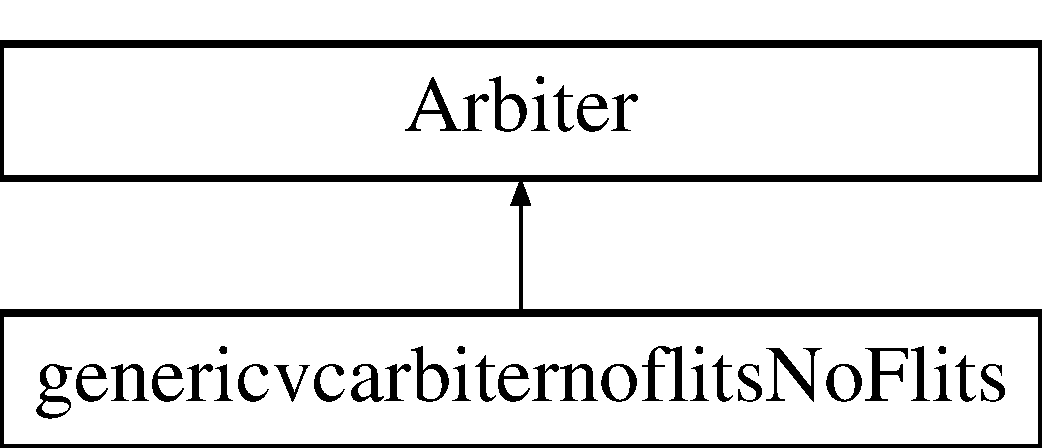
\includegraphics[height=2cm]{classgenericvcarbiternoflitsNoFlits}
\end{center}
\end{figure}
\subsection*{Public Member Functions}
\begin{CompactItemize}
\item 
\hyperlink{classgenericvcarbiternoflitsNoFlits_db66d29bba61a5e4bf3ef5ec5d61ce15}{genericvcarbiternoflitsNoFlits} ()
\item 
\hyperlink{classgenericvcarbiternoflitsNoFlits_337ead5b3dee13995af1c6636f7f3670}{$\sim$genericvcarbiternoflitsNoFlits} ()
\item 
bool \hyperlink{classgenericvcarbiternoflitsNoFlits_9a0299945d0e4d627534ffcfd06a8921}{is\_\-requested} (\hyperlink{outputBuffer_8h_91ad9478d81a7aaf2593e8d9c3d06a14}{uint} ch)
\item 
void \hyperlink{classgenericvcarbiternoflitsNoFlits_6d61b38c12a4dcae8137849232106541}{set\_\-no\_\-vcs} (\hyperlink{outputBuffer_8h_91ad9478d81a7aaf2593e8d9c3d06a14}{uint} ch)
\item 
void \hyperlink{classgenericvcarbiternoflitsNoFlits_679b8b6bc3be8c5e28635939a10ee2b7}{request} (\hyperlink{outputBuffer_8h_91ad9478d81a7aaf2593e8d9c3d06a14}{uint} ch)
\item 
\hyperlink{outputBuffer_8h_91ad9478d81a7aaf2593e8d9c3d06a14}{uint} \hyperlink{classgenericvcarbiternoflitsNoFlits_21ef6c560a4408fb9233416f384ec434}{get\_\-no\_\-requests} ()
\item 
\hyperlink{outputBuffer_8h_91ad9478d81a7aaf2593e8d9c3d06a14}{uint} \hyperlink{classgenericvcarbiternoflitsNoFlits_8d28e69dbcb2e4bd1bce785ade0b4573}{pick\_\-winner} ()
\item 
string \hyperlink{classgenericvcarbiternoflitsNoFlits_0cbe88bbc52325a3f4301bcca576e2ea}{toString} () const 
\item 
void \hyperlink{classgenericvcarbiternoflitsNoFlits_27217b32212845d3c7e3dfe4a87715c4}{clear\_\-winner} ()
\end{CompactItemize}
\subsection*{Public Attributes}
\begin{CompactItemize}
\item 
\hyperlink{outputBuffer_8h_91ad9478d81a7aaf2593e8d9c3d06a14}{uint} \hyperlink{classgenericvcarbiternoflitsNoFlits_17c531b8bb9df1098347bdfdf50f8bc9}{node\_\-ip}
\item 
\hyperlink{outputBuffer_8h_91ad9478d81a7aaf2593e8d9c3d06a14}{uint} \hyperlink{classgenericvcarbiternoflitsNoFlits_5160d84b65185cfc3d7942ebb186982c}{address}
\item 
string \hyperlink{classgenericvcarbiternoflitsNoFlits_9f7e29c9d9d8568b3178082ed6c76f4e}{name}
\end{CompactItemize}


\subsection{Constructor \& Destructor Documentation}
\hypertarget{classgenericvcarbiternoflitsNoFlits_db66d29bba61a5e4bf3ef5ec5d61ce15}{
\index{genericvcarbiternoflitsNoFlits@{genericvcarbiternoflitsNoFlits}!genericvcarbiternoflitsNoFlits@{genericvcarbiternoflitsNoFlits}}
\index{genericvcarbiternoflitsNoFlits@{genericvcarbiternoflitsNoFlits}!genericvcarbiternoflitsNoFlits@{genericvcarbiternoflitsNoFlits}}
\subsubsection[{genericvcarbiternoflitsNoFlits}]{\setlength{\rightskip}{0pt plus 5cm}genericvcarbiternoflitsNoFlits::genericvcarbiternoflitsNoFlits ()}}
\label{classgenericvcarbiternoflitsNoFlits_db66d29bba61a5e4bf3ef5ec5d61ce15}


\hypertarget{classgenericvcarbiternoflitsNoFlits_337ead5b3dee13995af1c6636f7f3670}{
\index{genericvcarbiternoflitsNoFlits@{genericvcarbiternoflitsNoFlits}!$\sim$genericvcarbiternoflitsNoFlits@{$\sim$genericvcarbiternoflitsNoFlits}}
\index{$\sim$genericvcarbiternoflitsNoFlits@{$\sim$genericvcarbiternoflitsNoFlits}!genericvcarbiternoflitsNoFlits@{genericvcarbiternoflitsNoFlits}}
\subsubsection[{$\sim$genericvcarbiternoflitsNoFlits}]{\setlength{\rightskip}{0pt plus 5cm}genericvcarbiternoflitsNoFlits::$\sim$genericvcarbiternoflitsNoFlits ()}}
\label{classgenericvcarbiternoflitsNoFlits_337ead5b3dee13995af1c6636f7f3670}




\subsection{Member Function Documentation}
\hypertarget{classgenericvcarbiternoflitsNoFlits_27217b32212845d3c7e3dfe4a87715c4}{
\index{genericvcarbiternoflitsNoFlits@{genericvcarbiternoflitsNoFlits}!clear\_\-winner@{clear\_\-winner}}
\index{clear\_\-winner@{clear\_\-winner}!genericvcarbiternoflitsNoFlits@{genericvcarbiternoflitsNoFlits}}
\subsubsection[{clear\_\-winner}]{\setlength{\rightskip}{0pt plus 5cm}void genericvcarbiternoflitsNoFlits::clear\_\-winner ()}}
\label{classgenericvcarbiternoflitsNoFlits_27217b32212845d3c7e3dfe4a87715c4}


\hypertarget{classgenericvcarbiternoflitsNoFlits_21ef6c560a4408fb9233416f384ec434}{
\index{genericvcarbiternoflitsNoFlits@{genericvcarbiternoflitsNoFlits}!get\_\-no\_\-requests@{get\_\-no\_\-requests}}
\index{get\_\-no\_\-requests@{get\_\-no\_\-requests}!genericvcarbiternoflitsNoFlits@{genericvcarbiternoflitsNoFlits}}
\subsubsection[{get\_\-no\_\-requests}]{\setlength{\rightskip}{0pt plus 5cm}{\bf uint} genericvcarbiternoflitsNoFlits::get\_\-no\_\-requests ()}}
\label{classgenericvcarbiternoflitsNoFlits_21ef6c560a4408fb9233416f384ec434}


\hypertarget{classgenericvcarbiternoflitsNoFlits_9a0299945d0e4d627534ffcfd06a8921}{
\index{genericvcarbiternoflitsNoFlits@{genericvcarbiternoflitsNoFlits}!is\_\-requested@{is\_\-requested}}
\index{is\_\-requested@{is\_\-requested}!genericvcarbiternoflitsNoFlits@{genericvcarbiternoflitsNoFlits}}
\subsubsection[{is\_\-requested}]{\setlength{\rightskip}{0pt plus 5cm}bool genericvcarbiternoflitsNoFlits::is\_\-requested ({\bf uint} {\em ch})}}
\label{classgenericvcarbiternoflitsNoFlits_9a0299945d0e4d627534ffcfd06a8921}


\hypertarget{classgenericvcarbiternoflitsNoFlits_8d28e69dbcb2e4bd1bce785ade0b4573}{
\index{genericvcarbiternoflitsNoFlits@{genericvcarbiternoflitsNoFlits}!pick\_\-winner@{pick\_\-winner}}
\index{pick\_\-winner@{pick\_\-winner}!genericvcarbiternoflitsNoFlits@{genericvcarbiternoflitsNoFlits}}
\subsubsection[{pick\_\-winner}]{\setlength{\rightskip}{0pt plus 5cm}{\bf uint} genericvcarbiternoflitsNoFlits::pick\_\-winner ()}}
\label{classgenericvcarbiternoflitsNoFlits_8d28e69dbcb2e4bd1bce785ade0b4573}


\hypertarget{classgenericvcarbiternoflitsNoFlits_679b8b6bc3be8c5e28635939a10ee2b7}{
\index{genericvcarbiternoflitsNoFlits@{genericvcarbiternoflitsNoFlits}!request@{request}}
\index{request@{request}!genericvcarbiternoflitsNoFlits@{genericvcarbiternoflitsNoFlits}}
\subsubsection[{request}]{\setlength{\rightskip}{0pt plus 5cm}void genericvcarbiternoflitsNoFlits::request ({\bf uint} {\em ch})}}
\label{classgenericvcarbiternoflitsNoFlits_679b8b6bc3be8c5e28635939a10ee2b7}


\hypertarget{classgenericvcarbiternoflitsNoFlits_6d61b38c12a4dcae8137849232106541}{
\index{genericvcarbiternoflitsNoFlits@{genericvcarbiternoflitsNoFlits}!set\_\-no\_\-vcs@{set\_\-no\_\-vcs}}
\index{set\_\-no\_\-vcs@{set\_\-no\_\-vcs}!genericvcarbiternoflitsNoFlits@{genericvcarbiternoflitsNoFlits}}
\subsubsection[{set\_\-no\_\-vcs}]{\setlength{\rightskip}{0pt plus 5cm}void genericvcarbiternoflitsNoFlits::set\_\-no\_\-vcs ({\bf uint} {\em ch})}}
\label{classgenericvcarbiternoflitsNoFlits_6d61b38c12a4dcae8137849232106541}


\hypertarget{classgenericvcarbiternoflitsNoFlits_0cbe88bbc52325a3f4301bcca576e2ea}{
\index{genericvcarbiternoflitsNoFlits@{genericvcarbiternoflitsNoFlits}!toString@{toString}}
\index{toString@{toString}!genericvcarbiternoflitsNoFlits@{genericvcarbiternoflitsNoFlits}}
\subsubsection[{toString}]{\setlength{\rightskip}{0pt plus 5cm}string genericvcarbiternoflitsNoFlits::toString () const}}
\label{classgenericvcarbiternoflitsNoFlits_0cbe88bbc52325a3f4301bcca576e2ea}




\subsection{Member Data Documentation}
\hypertarget{classgenericvcarbiternoflitsNoFlits_5160d84b65185cfc3d7942ebb186982c}{
\index{genericvcarbiternoflitsNoFlits@{genericvcarbiternoflitsNoFlits}!address@{address}}
\index{address@{address}!genericvcarbiternoflitsNoFlits@{genericvcarbiternoflitsNoFlits}}
\subsubsection[{address}]{\setlength{\rightskip}{0pt plus 5cm}{\bf uint} {\bf genericvcarbiternoflitsNoFlits::address}}}
\label{classgenericvcarbiternoflitsNoFlits_5160d84b65185cfc3d7942ebb186982c}


\hypertarget{classgenericvcarbiternoflitsNoFlits_9f7e29c9d9d8568b3178082ed6c76f4e}{
\index{genericvcarbiternoflitsNoFlits@{genericvcarbiternoflitsNoFlits}!name@{name}}
\index{name@{name}!genericvcarbiternoflitsNoFlits@{genericvcarbiternoflitsNoFlits}}
\subsubsection[{name}]{\setlength{\rightskip}{0pt plus 5cm}string {\bf genericvcarbiternoflitsNoFlits::name}}}
\label{classgenericvcarbiternoflitsNoFlits_9f7e29c9d9d8568b3178082ed6c76f4e}


\hypertarget{classgenericvcarbiternoflitsNoFlits_17c531b8bb9df1098347bdfdf50f8bc9}{
\index{genericvcarbiternoflitsNoFlits@{genericvcarbiternoflitsNoFlits}!node\_\-ip@{node\_\-ip}}
\index{node\_\-ip@{node\_\-ip}!genericvcarbiternoflitsNoFlits@{genericvcarbiternoflitsNoFlits}}
\subsubsection[{node\_\-ip}]{\setlength{\rightskip}{0pt plus 5cm}{\bf uint} {\bf genericvcarbiternoflitsNoFlits::node\_\-ip}}}
\label{classgenericvcarbiternoflitsNoFlits_17c531b8bb9df1098347bdfdf50f8bc9}




The documentation for this class was generated from the following files:\begin{CompactItemize}
\item 
source/components/impl/\hyperlink{genericVcArbiterNoFlits_8h}{genericVcArbiterNoFlits.h}\item 
source/components/impl/\hyperlink{genericVcArbiterNoFlits_8cc}{genericVcArbiterNoFlits.cc}\end{CompactItemize}

\hypertarget{classHeadFlit}{
\section{HeadFlit Class Reference}
\label{classHeadFlit}\index{HeadFlit@{HeadFlit}}
}
{\tt \#include $<$flit.h$>$}

Inheritance diagram for HeadFlit::\begin{figure}[H]
\begin{center}
\leavevmode
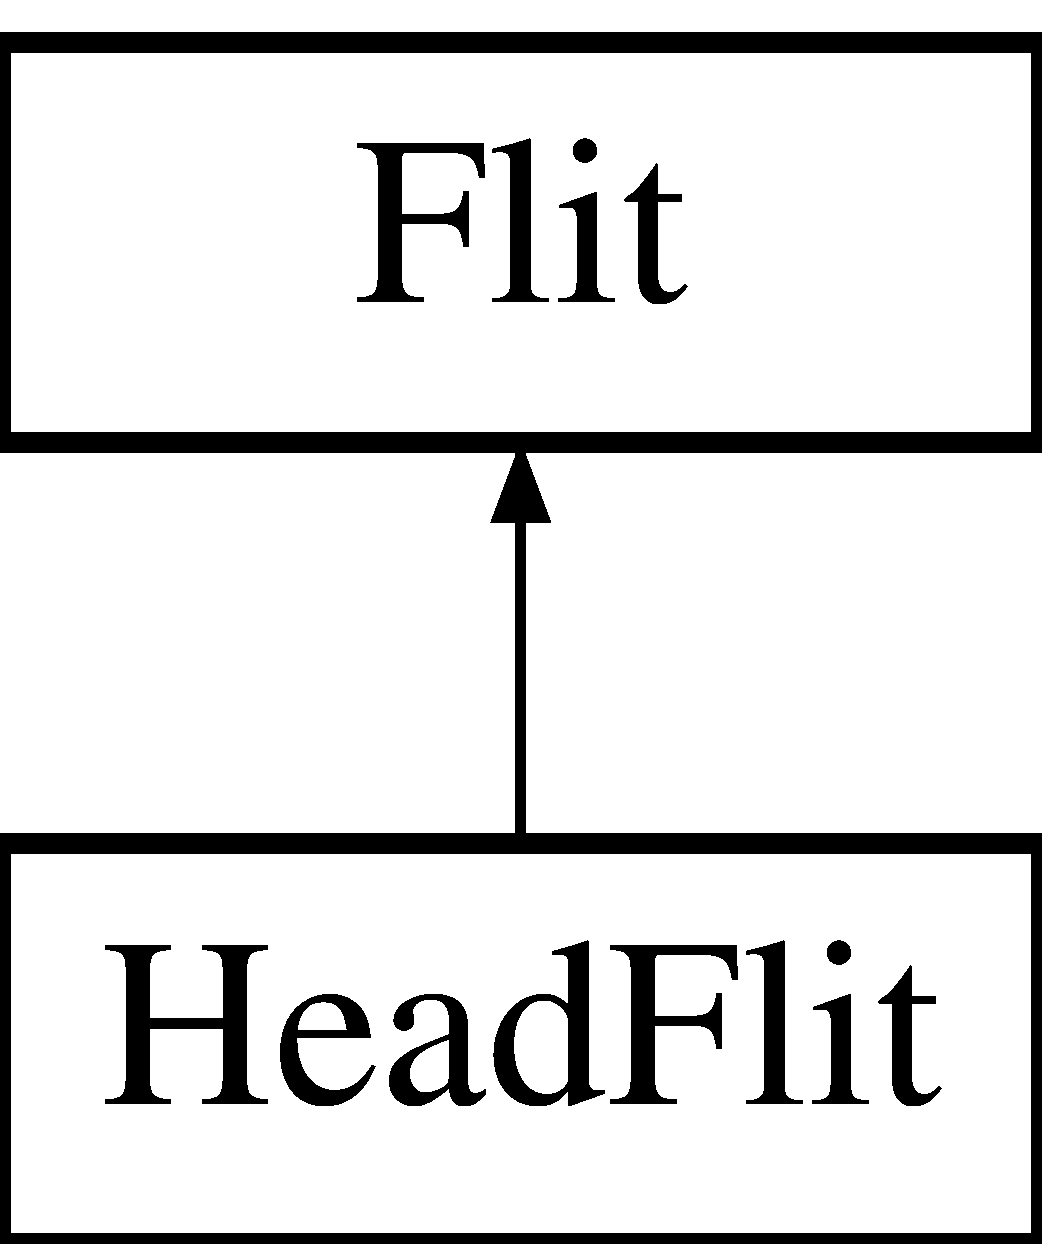
\includegraphics[height=2cm]{classHeadFlit}
\end{center}
\end{figure}
\subsection*{Public Member Functions}
\begin{CompactItemize}
\item 
\hyperlink{classHeadFlit_f7e40d1eb615c1950daec0044e103d14}{HeadFlit} ()
\item 
\hyperlink{classHeadFlit_baed314fc6d83dc45b11bc8154de9060}{$\sim$HeadFlit} ()
\item 
void \hyperlink{classHeadFlit_6a0b5e2ddf99c2722b2d06ca103707f8}{populate\_\-head\_\-flit} ()
\item 
string \hyperlink{classHeadFlit_4d22ac839cad2ac7ef0aedfeb54c9421}{toString} () const 
\item 
void \hyperlink{classHeadFlit_45b1f981d63ba53d1814250cc7efa9a4}{route} ()
\item 
pair$<$ \hyperlink{outputBuffer_8h_91ad9478d81a7aaf2593e8d9c3d06a14}{uint}, \hyperlink{outputBuffer_8h_91ad9478d81a7aaf2593e8d9c3d06a14}{uint} $>$ \hyperlink{classHeadFlit_ad973bdd54d38ac2a5ad05e27d3066f1}{next} ()
\end{CompactItemize}
\subsection*{Public Attributes}
\begin{CompactItemize}
\item 
\hyperlink{outputBuffer_8h_91ad9478d81a7aaf2593e8d9c3d06a14}{uint} \hyperlink{classHeadFlit_d7e8fd576ead55e392185a75da63aca1}{src\_\-address}
\item 
\hyperlink{outputBuffer_8h_91ad9478d81a7aaf2593e8d9c3d06a14}{uint} \hyperlink{classHeadFlit_1c5bf74e402bfa95645fb9cb4d188798}{dst\_\-address}
\item 
\hyperlink{outputBuffer_8h_91ad9478d81a7aaf2593e8d9c3d06a14}{uint} \hyperlink{classHeadFlit_4dd44bd07942e1eeace24cae293beb5a}{transaction\_\-id}
\item 
\hyperlink{outputBuffer_8h_91ad9478d81a7aaf2593e8d9c3d06a14}{uint} \hyperlink{classHeadFlit_b506d4907576fce81b277b30995e9867}{length}
\item 
vector$<$ bool $>$ \hyperlink{classHeadFlit_96e3a75d0e2d04fb465e4b7463e7325e}{control\_\-bits}
\end{CompactItemize}


\subsection{Constructor \& Destructor Documentation}
\hypertarget{classHeadFlit_f7e40d1eb615c1950daec0044e103d14}{
\index{HeadFlit@{HeadFlit}!HeadFlit@{HeadFlit}}
\index{HeadFlit@{HeadFlit}!HeadFlit@{HeadFlit}}
\subsubsection[{HeadFlit}]{\setlength{\rightskip}{0pt plus 5cm}HeadFlit::HeadFlit ()}}
\label{classHeadFlit_f7e40d1eb615c1950daec0044e103d14}


\hypertarget{classHeadFlit_baed314fc6d83dc45b11bc8154de9060}{
\index{HeadFlit@{HeadFlit}!$\sim$HeadFlit@{$\sim$HeadFlit}}
\index{$\sim$HeadFlit@{$\sim$HeadFlit}!HeadFlit@{HeadFlit}}
\subsubsection[{$\sim$HeadFlit}]{\setlength{\rightskip}{0pt plus 5cm}HeadFlit::$\sim$HeadFlit ()}}
\label{classHeadFlit_baed314fc6d83dc45b11bc8154de9060}




\subsection{Member Function Documentation}
\hypertarget{classHeadFlit_ad973bdd54d38ac2a5ad05e27d3066f1}{
\index{HeadFlit@{HeadFlit}!next@{next}}
\index{next@{next}!HeadFlit@{HeadFlit}}
\subsubsection[{next}]{\setlength{\rightskip}{0pt plus 5cm}pair$<${\bf uint}, {\bf uint}$>$ HeadFlit::next ()}}
\label{classHeadFlit_ad973bdd54d38ac2a5ad05e27d3066f1}


\hypertarget{classHeadFlit_6a0b5e2ddf99c2722b2d06ca103707f8}{
\index{HeadFlit@{HeadFlit}!populate\_\-head\_\-flit@{populate\_\-head\_\-flit}}
\index{populate\_\-head\_\-flit@{populate\_\-head\_\-flit}!HeadFlit@{HeadFlit}}
\subsubsection[{populate\_\-head\_\-flit}]{\setlength{\rightskip}{0pt plus 5cm}void HeadFlit::populate\_\-head\_\-flit ()}}
\label{classHeadFlit_6a0b5e2ddf99c2722b2d06ca103707f8}


\hypertarget{classHeadFlit_45b1f981d63ba53d1814250cc7efa9a4}{
\index{HeadFlit@{HeadFlit}!route@{route}}
\index{route@{route}!HeadFlit@{HeadFlit}}
\subsubsection[{route}]{\setlength{\rightskip}{0pt plus 5cm}void HeadFlit::route ()}}
\label{classHeadFlit_45b1f981d63ba53d1814250cc7efa9a4}


\hypertarget{classHeadFlit_4d22ac839cad2ac7ef0aedfeb54c9421}{
\index{HeadFlit@{HeadFlit}!toString@{toString}}
\index{toString@{toString}!HeadFlit@{HeadFlit}}
\subsubsection[{toString}]{\setlength{\rightskip}{0pt plus 5cm}string HeadFlit::toString () const}}
\label{classHeadFlit_4d22ac839cad2ac7ef0aedfeb54c9421}




Reimplemented from \hyperlink{classFlit_ffc6c729a005389b51818aac59710dab}{Flit}.

\subsection{Member Data Documentation}
\hypertarget{classHeadFlit_96e3a75d0e2d04fb465e4b7463e7325e}{
\index{HeadFlit@{HeadFlit}!control\_\-bits@{control\_\-bits}}
\index{control\_\-bits@{control\_\-bits}!HeadFlit@{HeadFlit}}
\subsubsection[{control\_\-bits}]{\setlength{\rightskip}{0pt plus 5cm}vector$<$bool$>$ {\bf HeadFlit::control\_\-bits}}}
\label{classHeadFlit_96e3a75d0e2d04fb465e4b7463e7325e}


\hypertarget{classHeadFlit_1c5bf74e402bfa95645fb9cb4d188798}{
\index{HeadFlit@{HeadFlit}!dst\_\-address@{dst\_\-address}}
\index{dst\_\-address@{dst\_\-address}!HeadFlit@{HeadFlit}}
\subsubsection[{dst\_\-address}]{\setlength{\rightskip}{0pt plus 5cm}{\bf uint} {\bf HeadFlit::dst\_\-address}}}
\label{classHeadFlit_1c5bf74e402bfa95645fb9cb4d188798}


\hypertarget{classHeadFlit_b506d4907576fce81b277b30995e9867}{
\index{HeadFlit@{HeadFlit}!length@{length}}
\index{length@{length}!HeadFlit@{HeadFlit}}
\subsubsection[{length}]{\setlength{\rightskip}{0pt plus 5cm}{\bf uint} {\bf HeadFlit::length}}}
\label{classHeadFlit_b506d4907576fce81b277b30995e9867}


\hypertarget{classHeadFlit_d7e8fd576ead55e392185a75da63aca1}{
\index{HeadFlit@{HeadFlit}!src\_\-address@{src\_\-address}}
\index{src\_\-address@{src\_\-address}!HeadFlit@{HeadFlit}}
\subsubsection[{src\_\-address}]{\setlength{\rightskip}{0pt plus 5cm}{\bf uint} {\bf HeadFlit::src\_\-address}}}
\label{classHeadFlit_d7e8fd576ead55e392185a75da63aca1}


\hypertarget{classHeadFlit_4dd44bd07942e1eeace24cae293beb5a}{
\index{HeadFlit@{HeadFlit}!transaction\_\-id@{transaction\_\-id}}
\index{transaction\_\-id@{transaction\_\-id}!HeadFlit@{HeadFlit}}
\subsubsection[{transaction\_\-id}]{\setlength{\rightskip}{0pt plus 5cm}{\bf uint} {\bf HeadFlit::transaction\_\-id}}}
\label{classHeadFlit_4dd44bd07942e1eeace24cae293beb5a}




The documentation for this class was generated from the following files:\begin{CompactItemize}
\item 
source/data\_\-types/impl/\hyperlink{flit_8h}{flit.h}\item 
source/data\_\-types/impl/\hyperlink{flit_8cc}{flit.cc}\end{CompactItemize}

\hypertarget{classHighLevelPacket}{
\section{HighLevelPacket Class Reference}
\label{classHighLevelPacket}\index{HighLevelPacket@{HighLevelPacket}}
}
{\tt \#include $<$highLevelPacket.h$>$}

\subsection*{Public Member Functions}
\begin{CompactItemize}
\item 
\hyperlink{classHighLevelPacket_e6f7a4ec429537928d24f6a2199a3f8d}{HighLevelPacket} ()
\item 
\hyperlink{classHighLevelPacket_dc29e5ebbbb6e7c3b1d1a53b0ea14142}{$\sim$HighLevelPacket} ()
\item 
\hyperlink{genericComponentHeader_8h_d88faca783e7aa496cda721d9029a2e3}{simTime} \hyperlink{classHighLevelPacket_0ddd2a5fd2195c2ce43198c82163522c}{get\_\-transit\_\-time} ()
\item 
void \hyperlink{classHighLevelPacket_03017f87443d346d08e8ebb4281073c1}{to\_\-low\_\-level\_\-packet} (\hyperlink{classLowLevelPacket}{LowLevelPacket} $\ast$llp)
\item 
void \hyperlink{classHighLevelPacket_6a4e25020ea0c66aab015e9c2a2c8c85}{from\_\-low\_\-level\_\-packet} (\hyperlink{classLowLevelPacket}{LowLevelPacket} $\ast$llp)
\item 
string \hyperlink{classHighLevelPacket_a2292ef0554d515cf08aeed8ca46d419}{toString} () const 
\item 
bool \hyperlink{classHighLevelPacket_08e3560b71bab8b1ff31844d8ddff819}{operator==} (const \hyperlink{classHighLevelPacket}{HighLevelPacket} $\ast$p)
\end{CompactItemize}
\subsection*{Public Attributes}
\begin{CompactItemize}
\item 
\hyperlink{outputBuffer_8h_91ad9478d81a7aaf2593e8d9c3d06a14}{uint} \hyperlink{classHighLevelPacket_d09485039d19ea9f0f58697e9fdf6450}{source}
\item 
\hyperlink{outputBuffer_8h_91ad9478d81a7aaf2593e8d9c3d06a14}{uint} \hyperlink{classHighLevelPacket_abe7a75c784f1824211ba194819e0d4e}{destination}
\item 
\hyperlink{highLevelPacket_8h_2f11671ee174f5c324e71f348aef6e96}{virtual\_\-network} \hyperlink{classHighLevelPacket_0e554b43c609ab77758300f332679a29}{vn}
\item 
\hyperlink{highLevelPacket_8h_155eefa40b3e6db305cb151f7bb6bef4}{message\_\-class} \hyperlink{classHighLevelPacket_4bddc51ad584c87c2241b800f6b2f0c9}{mc}
\item 
\hyperlink{outputBuffer_8h_91ad9478d81a7aaf2593e8d9c3d06a14}{uint} \hyperlink{classHighLevelPacket_0e369f54800e9bb403f8277b94cbaa96}{virtual\_\-channel}
\item 
\hyperlink{outputBuffer_8h_91ad9478d81a7aaf2593e8d9c3d06a14}{uint} \hyperlink{classHighLevelPacket_287c21f9e31f882ffe8c8ff353dab087}{transaction\_\-id}
\item 
\hyperlink{genericComponentHeader_8h_d88faca783e7aa496cda721d9029a2e3}{simTime} \hyperlink{classHighLevelPacket_eed2f14fb0b689f35a92c054a831867c}{sent\_\-time}
\item 
\hyperlink{genericComponentHeader_8h_d88faca783e7aa496cda721d9029a2e3}{simTime} \hyperlink{classHighLevelPacket_5de1d4d144aa5e9fdac1a3988384d92f}{recv\_\-time}
\item 
unsigned int \hyperlink{classHighLevelPacket_c7bf05e9b1560991d60ca12fd0d309a3}{data\_\-payload\_\-length}
\item 
vector$<$ bool $>$ \hyperlink{classHighLevelPacket_340b7688df206e49a62301e2dae093de}{data}
\end{CompactItemize}


\subsection{Constructor \& Destructor Documentation}
\hypertarget{classHighLevelPacket_e6f7a4ec429537928d24f6a2199a3f8d}{
\index{HighLevelPacket@{HighLevelPacket}!HighLevelPacket@{HighLevelPacket}}
\index{HighLevelPacket@{HighLevelPacket}!HighLevelPacket@{HighLevelPacket}}
\subsubsection[{HighLevelPacket}]{\setlength{\rightskip}{0pt plus 5cm}HighLevelPacket::HighLevelPacket ()}}
\label{classHighLevelPacket_e6f7a4ec429537928d24f6a2199a3f8d}


\hypertarget{classHighLevelPacket_dc29e5ebbbb6e7c3b1d1a53b0ea14142}{
\index{HighLevelPacket@{HighLevelPacket}!$\sim$HighLevelPacket@{$\sim$HighLevelPacket}}
\index{$\sim$HighLevelPacket@{$\sim$HighLevelPacket}!HighLevelPacket@{HighLevelPacket}}
\subsubsection[{$\sim$HighLevelPacket}]{\setlength{\rightskip}{0pt plus 5cm}HighLevelPacket::$\sim$HighLevelPacket ()}}
\label{classHighLevelPacket_dc29e5ebbbb6e7c3b1d1a53b0ea14142}




\subsection{Member Function Documentation}
\hypertarget{classHighLevelPacket_6a4e25020ea0c66aab015e9c2a2c8c85}{
\index{HighLevelPacket@{HighLevelPacket}!from\_\-low\_\-level\_\-packet@{from\_\-low\_\-level\_\-packet}}
\index{from\_\-low\_\-level\_\-packet@{from\_\-low\_\-level\_\-packet}!HighLevelPacket@{HighLevelPacket}}
\subsubsection[{from\_\-low\_\-level\_\-packet}]{\setlength{\rightskip}{0pt plus 5cm}void HighLevelPacket::from\_\-low\_\-level\_\-packet ({\bf LowLevelPacket} $\ast$ {\em llp})}}
\label{classHighLevelPacket_6a4e25020ea0c66aab015e9c2a2c8c85}


\hypertarget{classHighLevelPacket_0ddd2a5fd2195c2ce43198c82163522c}{
\index{HighLevelPacket@{HighLevelPacket}!get\_\-transit\_\-time@{get\_\-transit\_\-time}}
\index{get\_\-transit\_\-time@{get\_\-transit\_\-time}!HighLevelPacket@{HighLevelPacket}}
\subsubsection[{get\_\-transit\_\-time}]{\setlength{\rightskip}{0pt plus 5cm}{\bf simTime} HighLevelPacket::get\_\-transit\_\-time ()}}
\label{classHighLevelPacket_0ddd2a5fd2195c2ce43198c82163522c}


\hypertarget{classHighLevelPacket_08e3560b71bab8b1ff31844d8ddff819}{
\index{HighLevelPacket@{HighLevelPacket}!operator==@{operator==}}
\index{operator==@{operator==}!HighLevelPacket@{HighLevelPacket}}
\subsubsection[{operator==}]{\setlength{\rightskip}{0pt plus 5cm}bool HighLevelPacket::operator== (const {\bf HighLevelPacket} $\ast$ {\em p})}}
\label{classHighLevelPacket_08e3560b71bab8b1ff31844d8ddff819}


\hypertarget{classHighLevelPacket_03017f87443d346d08e8ebb4281073c1}{
\index{HighLevelPacket@{HighLevelPacket}!to\_\-low\_\-level\_\-packet@{to\_\-low\_\-level\_\-packet}}
\index{to\_\-low\_\-level\_\-packet@{to\_\-low\_\-level\_\-packet}!HighLevelPacket@{HighLevelPacket}}
\subsubsection[{to\_\-low\_\-level\_\-packet}]{\setlength{\rightskip}{0pt plus 5cm}void HighLevelPacket::to\_\-low\_\-level\_\-packet ({\bf LowLevelPacket} $\ast$ {\em llp})}}
\label{classHighLevelPacket_03017f87443d346d08e8ebb4281073c1}


\hypertarget{classHighLevelPacket_a2292ef0554d515cf08aeed8ca46d419}{
\index{HighLevelPacket@{HighLevelPacket}!toString@{toString}}
\index{toString@{toString}!HighLevelPacket@{HighLevelPacket}}
\subsubsection[{toString}]{\setlength{\rightskip}{0pt plus 5cm}string HighLevelPacket::toString () const}}
\label{classHighLevelPacket_a2292ef0554d515cf08aeed8ca46d419}




\subsection{Member Data Documentation}
\hypertarget{classHighLevelPacket_340b7688df206e49a62301e2dae093de}{
\index{HighLevelPacket@{HighLevelPacket}!data@{data}}
\index{data@{data}!HighLevelPacket@{HighLevelPacket}}
\subsubsection[{data}]{\setlength{\rightskip}{0pt plus 5cm}vector$<$bool$>$ {\bf HighLevelPacket::data}}}
\label{classHighLevelPacket_340b7688df206e49a62301e2dae093de}


\hypertarget{classHighLevelPacket_c7bf05e9b1560991d60ca12fd0d309a3}{
\index{HighLevelPacket@{HighLevelPacket}!data\_\-payload\_\-length@{data\_\-payload\_\-length}}
\index{data\_\-payload\_\-length@{data\_\-payload\_\-length}!HighLevelPacket@{HighLevelPacket}}
\subsubsection[{data\_\-payload\_\-length}]{\setlength{\rightskip}{0pt plus 5cm}unsigned int {\bf HighLevelPacket::data\_\-payload\_\-length}}}
\label{classHighLevelPacket_c7bf05e9b1560991d60ca12fd0d309a3}


\hypertarget{classHighLevelPacket_abe7a75c784f1824211ba194819e0d4e}{
\index{HighLevelPacket@{HighLevelPacket}!destination@{destination}}
\index{destination@{destination}!HighLevelPacket@{HighLevelPacket}}
\subsubsection[{destination}]{\setlength{\rightskip}{0pt plus 5cm}{\bf uint} {\bf HighLevelPacket::destination}}}
\label{classHighLevelPacket_abe7a75c784f1824211ba194819e0d4e}


\hypertarget{classHighLevelPacket_4bddc51ad584c87c2241b800f6b2f0c9}{
\index{HighLevelPacket@{HighLevelPacket}!mc@{mc}}
\index{mc@{mc}!HighLevelPacket@{HighLevelPacket}}
\subsubsection[{mc}]{\setlength{\rightskip}{0pt plus 5cm}{\bf message\_\-class} {\bf HighLevelPacket::mc}}}
\label{classHighLevelPacket_4bddc51ad584c87c2241b800f6b2f0c9}


\hypertarget{classHighLevelPacket_5de1d4d144aa5e9fdac1a3988384d92f}{
\index{HighLevelPacket@{HighLevelPacket}!recv\_\-time@{recv\_\-time}}
\index{recv\_\-time@{recv\_\-time}!HighLevelPacket@{HighLevelPacket}}
\subsubsection[{recv\_\-time}]{\setlength{\rightskip}{0pt plus 5cm}{\bf simTime} {\bf HighLevelPacket::recv\_\-time}}}
\label{classHighLevelPacket_5de1d4d144aa5e9fdac1a3988384d92f}


\hypertarget{classHighLevelPacket_eed2f14fb0b689f35a92c054a831867c}{
\index{HighLevelPacket@{HighLevelPacket}!sent\_\-time@{sent\_\-time}}
\index{sent\_\-time@{sent\_\-time}!HighLevelPacket@{HighLevelPacket}}
\subsubsection[{sent\_\-time}]{\setlength{\rightskip}{0pt plus 5cm}{\bf simTime} {\bf HighLevelPacket::sent\_\-time}}}
\label{classHighLevelPacket_eed2f14fb0b689f35a92c054a831867c}


\hypertarget{classHighLevelPacket_d09485039d19ea9f0f58697e9fdf6450}{
\index{HighLevelPacket@{HighLevelPacket}!source@{source}}
\index{source@{source}!HighLevelPacket@{HighLevelPacket}}
\subsubsection[{source}]{\setlength{\rightskip}{0pt plus 5cm}{\bf uint} {\bf HighLevelPacket::source}}}
\label{classHighLevelPacket_d09485039d19ea9f0f58697e9fdf6450}


\hypertarget{classHighLevelPacket_287c21f9e31f882ffe8c8ff353dab087}{
\index{HighLevelPacket@{HighLevelPacket}!transaction\_\-id@{transaction\_\-id}}
\index{transaction\_\-id@{transaction\_\-id}!HighLevelPacket@{HighLevelPacket}}
\subsubsection[{transaction\_\-id}]{\setlength{\rightskip}{0pt plus 5cm}{\bf uint} {\bf HighLevelPacket::transaction\_\-id}}}
\label{classHighLevelPacket_287c21f9e31f882ffe8c8ff353dab087}


\hypertarget{classHighLevelPacket_0e369f54800e9bb403f8277b94cbaa96}{
\index{HighLevelPacket@{HighLevelPacket}!virtual\_\-channel@{virtual\_\-channel}}
\index{virtual\_\-channel@{virtual\_\-channel}!HighLevelPacket@{HighLevelPacket}}
\subsubsection[{virtual\_\-channel}]{\setlength{\rightskip}{0pt plus 5cm}{\bf uint} {\bf HighLevelPacket::virtual\_\-channel}}}
\label{classHighLevelPacket_0e369f54800e9bb403f8277b94cbaa96}


\hypertarget{classHighLevelPacket_0e554b43c609ab77758300f332679a29}{
\index{HighLevelPacket@{HighLevelPacket}!vn@{vn}}
\index{vn@{vn}!HighLevelPacket@{HighLevelPacket}}
\subsubsection[{vn}]{\setlength{\rightskip}{0pt plus 5cm}{\bf virtual\_\-network} {\bf HighLevelPacket::vn}}}
\label{classHighLevelPacket_0e554b43c609ab77758300f332679a29}




The documentation for this class was generated from the following files:\begin{CompactItemize}
\item 
source/data\_\-types/impl/\hyperlink{highLevelPacket_8h}{highLevelPacket.h}\item 
source/data\_\-types/impl/\hyperlink{highLevelPacket_8cc}{highLevelPacket.cc}\end{CompactItemize}

\hypertarget{classInputBuffer}{
\section{InputBuffer Class Reference}
\label{classInputBuffer}\index{InputBuffer@{InputBuffer}}
}
{\tt \#include $<$inputBuffer.h$>$}

Inheritance diagram for InputBuffer::\begin{figure}[H]
\begin{center}
\leavevmode
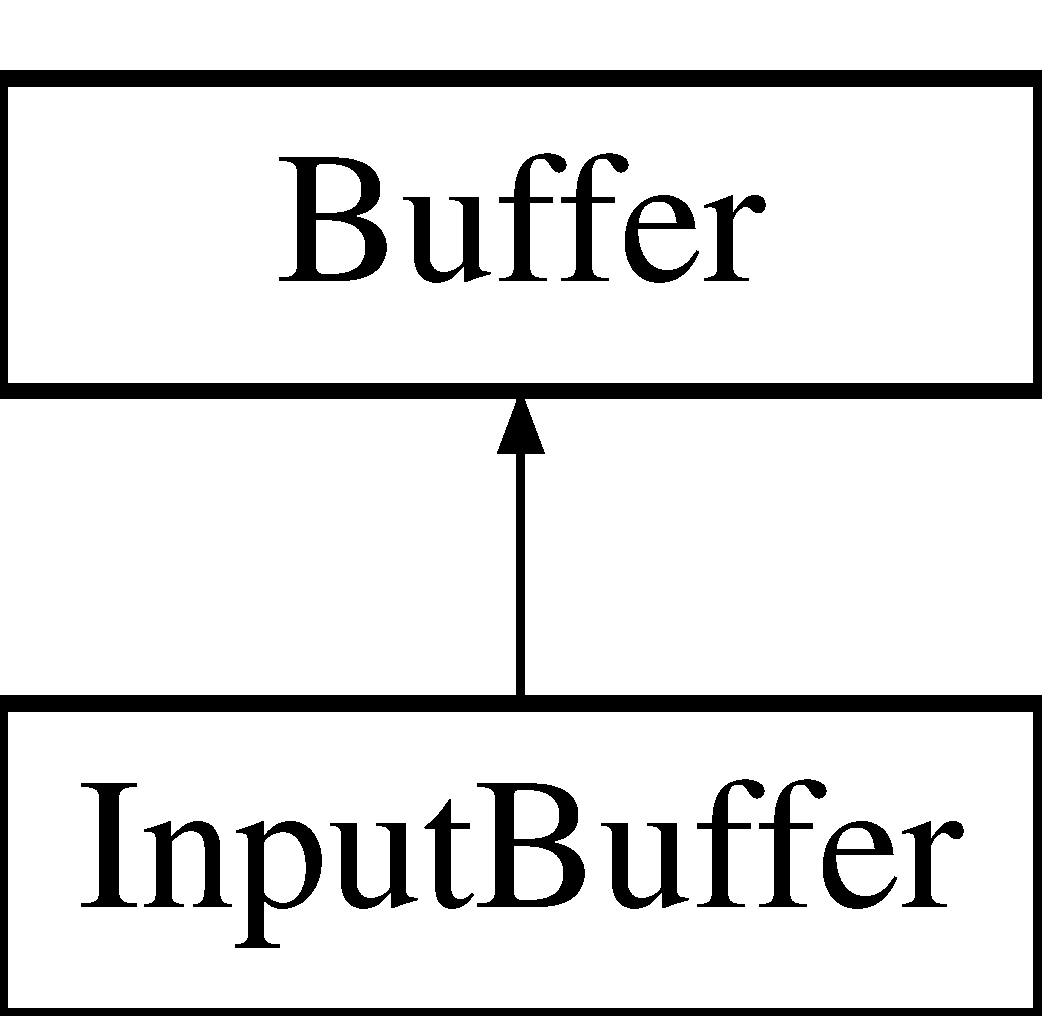
\includegraphics[height=2cm]{classInputBuffer}
\end{center}
\end{figure}
\subsection*{Public Member Functions}
\begin{CompactItemize}
\item 
\hyperlink{classInputBuffer_539e007478e6a19dd2c933e2fe6f6b5c}{InputBuffer} ()
\item 
virtual \hyperlink{classInputBuffer_c8e553cdc4097665450a7b83b797475c}{$\sim$InputBuffer} ()
\item 
virtual void \hyperlink{classInputBuffer_27ff9889e0ec93036b06b161f948bc8f}{set\_\-no\_\-vc} (\hyperlink{outputBuffer_8h_91ad9478d81a7aaf2593e8d9c3d06a14}{uint} vc)
\item 
virtual \hyperlink{outputBuffer_8h_91ad9478d81a7aaf2593e8d9c3d06a14}{uint} \hyperlink{classInputBuffer_2a76cc1cf7386e7d9bea7993660e7800}{get\_\-no\_\-vc} () const 
\item 
virtual void \hyperlink{classInputBuffer_86629ae58a881f42b19edfe07a53b8f0}{change\_\-pull\_\-channel} (\hyperlink{outputBuffer_8h_91ad9478d81a7aaf2593e8d9c3d06a14}{uint} channel)
\item 
virtual void \hyperlink{classInputBuffer_b63bf4f28edd8364edf000675bbf08ac}{change\_\-push\_\-channel} (\hyperlink{outputBuffer_8h_91ad9478d81a7aaf2593e8d9c3d06a14}{uint} channel)
\item 
virtual \hyperlink{outputBuffer_8h_91ad9478d81a7aaf2593e8d9c3d06a14}{uint} \hyperlink{classInputBuffer_b33dddf15a99bb33e22712b23c19cf82}{get\_\-pull\_\-channel} () const 
\item 
virtual \hyperlink{outputBuffer_8h_91ad9478d81a7aaf2593e8d9c3d06a14}{uint} \hyperlink{classInputBuffer_0c13c3b2a56799d78bf0961d74ad03a9}{get\_\-push\_\-channel} () const 
\item 
virtual bool \hyperlink{classInputBuffer_53d9799602c95d0b17b73e4b1d1b73d6}{is\_\-channel\_\-full} (\hyperlink{outputBuffer_8h_91ad9478d81a7aaf2593e8d9c3d06a14}{uint} channel) const 
\item 
virtual bool \hyperlink{classInputBuffer_bc130ab26e953ef77b7faa804388cb90}{is\_\-empty} (\hyperlink{outputBuffer_8h_91ad9478d81a7aaf2593e8d9c3d06a14}{uint} channel) const 
\end{CompactItemize}


\subsection{Constructor \& Destructor Documentation}
\hypertarget{classInputBuffer_539e007478e6a19dd2c933e2fe6f6b5c}{
\index{InputBuffer@{InputBuffer}!InputBuffer@{InputBuffer}}
\index{InputBuffer@{InputBuffer}!InputBuffer@{InputBuffer}}
\subsubsection[{InputBuffer}]{\setlength{\rightskip}{0pt plus 5cm}InputBuffer::InputBuffer ()\hspace{0.3cm}{\tt  \mbox{[}inline\mbox{]}}}}
\label{classInputBuffer_539e007478e6a19dd2c933e2fe6f6b5c}


\hypertarget{classInputBuffer_c8e553cdc4097665450a7b83b797475c}{
\index{InputBuffer@{InputBuffer}!$\sim$InputBuffer@{$\sim$InputBuffer}}
\index{$\sim$InputBuffer@{$\sim$InputBuffer}!InputBuffer@{InputBuffer}}
\subsubsection[{$\sim$InputBuffer}]{\setlength{\rightskip}{0pt plus 5cm}virtual InputBuffer::$\sim$InputBuffer ()\hspace{0.3cm}{\tt  \mbox{[}inline, virtual\mbox{]}}}}
\label{classInputBuffer_c8e553cdc4097665450a7b83b797475c}




\subsection{Member Function Documentation}
\hypertarget{classInputBuffer_86629ae58a881f42b19edfe07a53b8f0}{
\index{InputBuffer@{InputBuffer}!change\_\-pull\_\-channel@{change\_\-pull\_\-channel}}
\index{change\_\-pull\_\-channel@{change\_\-pull\_\-channel}!InputBuffer@{InputBuffer}}
\subsubsection[{change\_\-pull\_\-channel}]{\setlength{\rightskip}{0pt plus 5cm}virtual void InputBuffer::change\_\-pull\_\-channel ({\bf uint} {\em channel})\hspace{0.3cm}{\tt  \mbox{[}virtual\mbox{]}}}}
\label{classInputBuffer_86629ae58a881f42b19edfe07a53b8f0}


\hypertarget{classInputBuffer_b63bf4f28edd8364edf000675bbf08ac}{
\index{InputBuffer@{InputBuffer}!change\_\-push\_\-channel@{change\_\-push\_\-channel}}
\index{change\_\-push\_\-channel@{change\_\-push\_\-channel}!InputBuffer@{InputBuffer}}
\subsubsection[{change\_\-push\_\-channel}]{\setlength{\rightskip}{0pt plus 5cm}virtual void InputBuffer::change\_\-push\_\-channel ({\bf uint} {\em channel})\hspace{0.3cm}{\tt  \mbox{[}virtual\mbox{]}}}}
\label{classInputBuffer_b63bf4f28edd8364edf000675bbf08ac}


\hypertarget{classInputBuffer_2a76cc1cf7386e7d9bea7993660e7800}{
\index{InputBuffer@{InputBuffer}!get\_\-no\_\-vc@{get\_\-no\_\-vc}}
\index{get\_\-no\_\-vc@{get\_\-no\_\-vc}!InputBuffer@{InputBuffer}}
\subsubsection[{get\_\-no\_\-vc}]{\setlength{\rightskip}{0pt plus 5cm}virtual {\bf uint} InputBuffer::get\_\-no\_\-vc () const\hspace{0.3cm}{\tt  \mbox{[}virtual\mbox{]}}}}
\label{classInputBuffer_2a76cc1cf7386e7d9bea7993660e7800}


\hypertarget{classInputBuffer_b33dddf15a99bb33e22712b23c19cf82}{
\index{InputBuffer@{InputBuffer}!get\_\-pull\_\-channel@{get\_\-pull\_\-channel}}
\index{get\_\-pull\_\-channel@{get\_\-pull\_\-channel}!InputBuffer@{InputBuffer}}
\subsubsection[{get\_\-pull\_\-channel}]{\setlength{\rightskip}{0pt plus 5cm}virtual {\bf uint} InputBuffer::get\_\-pull\_\-channel () const\hspace{0.3cm}{\tt  \mbox{[}virtual\mbox{]}}}}
\label{classInputBuffer_b33dddf15a99bb33e22712b23c19cf82}


\hypertarget{classInputBuffer_0c13c3b2a56799d78bf0961d74ad03a9}{
\index{InputBuffer@{InputBuffer}!get\_\-push\_\-channel@{get\_\-push\_\-channel}}
\index{get\_\-push\_\-channel@{get\_\-push\_\-channel}!InputBuffer@{InputBuffer}}
\subsubsection[{get\_\-push\_\-channel}]{\setlength{\rightskip}{0pt plus 5cm}virtual {\bf uint} InputBuffer::get\_\-push\_\-channel () const\hspace{0.3cm}{\tt  \mbox{[}virtual\mbox{]}}}}
\label{classInputBuffer_0c13c3b2a56799d78bf0961d74ad03a9}


\hypertarget{classInputBuffer_53d9799602c95d0b17b73e4b1d1b73d6}{
\index{InputBuffer@{InputBuffer}!is\_\-channel\_\-full@{is\_\-channel\_\-full}}
\index{is\_\-channel\_\-full@{is\_\-channel\_\-full}!InputBuffer@{InputBuffer}}
\subsubsection[{is\_\-channel\_\-full}]{\setlength{\rightskip}{0pt plus 5cm}virtual bool InputBuffer::is\_\-channel\_\-full ({\bf uint} {\em channel}) const\hspace{0.3cm}{\tt  \mbox{[}virtual\mbox{]}}}}
\label{classInputBuffer_53d9799602c95d0b17b73e4b1d1b73d6}


\hypertarget{classInputBuffer_bc130ab26e953ef77b7faa804388cb90}{
\index{InputBuffer@{InputBuffer}!is\_\-empty@{is\_\-empty}}
\index{is\_\-empty@{is\_\-empty}!InputBuffer@{InputBuffer}}
\subsubsection[{is\_\-empty}]{\setlength{\rightskip}{0pt plus 5cm}virtual bool InputBuffer::is\_\-empty ({\bf uint} {\em channel}) const\hspace{0.3cm}{\tt  \mbox{[}virtual\mbox{]}}}}
\label{classInputBuffer_bc130ab26e953ef77b7faa804388cb90}


\hypertarget{classInputBuffer_27ff9889e0ec93036b06b161f948bc8f}{
\index{InputBuffer@{InputBuffer}!set\_\-no\_\-vc@{set\_\-no\_\-vc}}
\index{set\_\-no\_\-vc@{set\_\-no\_\-vc}!InputBuffer@{InputBuffer}}
\subsubsection[{set\_\-no\_\-vc}]{\setlength{\rightskip}{0pt plus 5cm}virtual void InputBuffer::set\_\-no\_\-vc ({\bf uint} {\em vc})\hspace{0.3cm}{\tt  \mbox{[}virtual\mbox{]}}}}
\label{classInputBuffer_27ff9889e0ec93036b06b161f948bc8f}




The documentation for this class was generated from the following file:\begin{CompactItemize}
\item 
source/components/interfaces/\hyperlink{inputBuffer_8h}{inputBuffer.h}\end{CompactItemize}

\hypertarget{classIntEmpirical}{
\section{IntEmpirical Class Reference}
\label{classIntEmpirical}\index{IntEmpirical@{IntEmpirical}}
}
{\tt \#include $<$rng.hpp$>$}

Inheritance diagram for IntEmpirical::\begin{figure}[H]
\begin{center}
\leavevmode
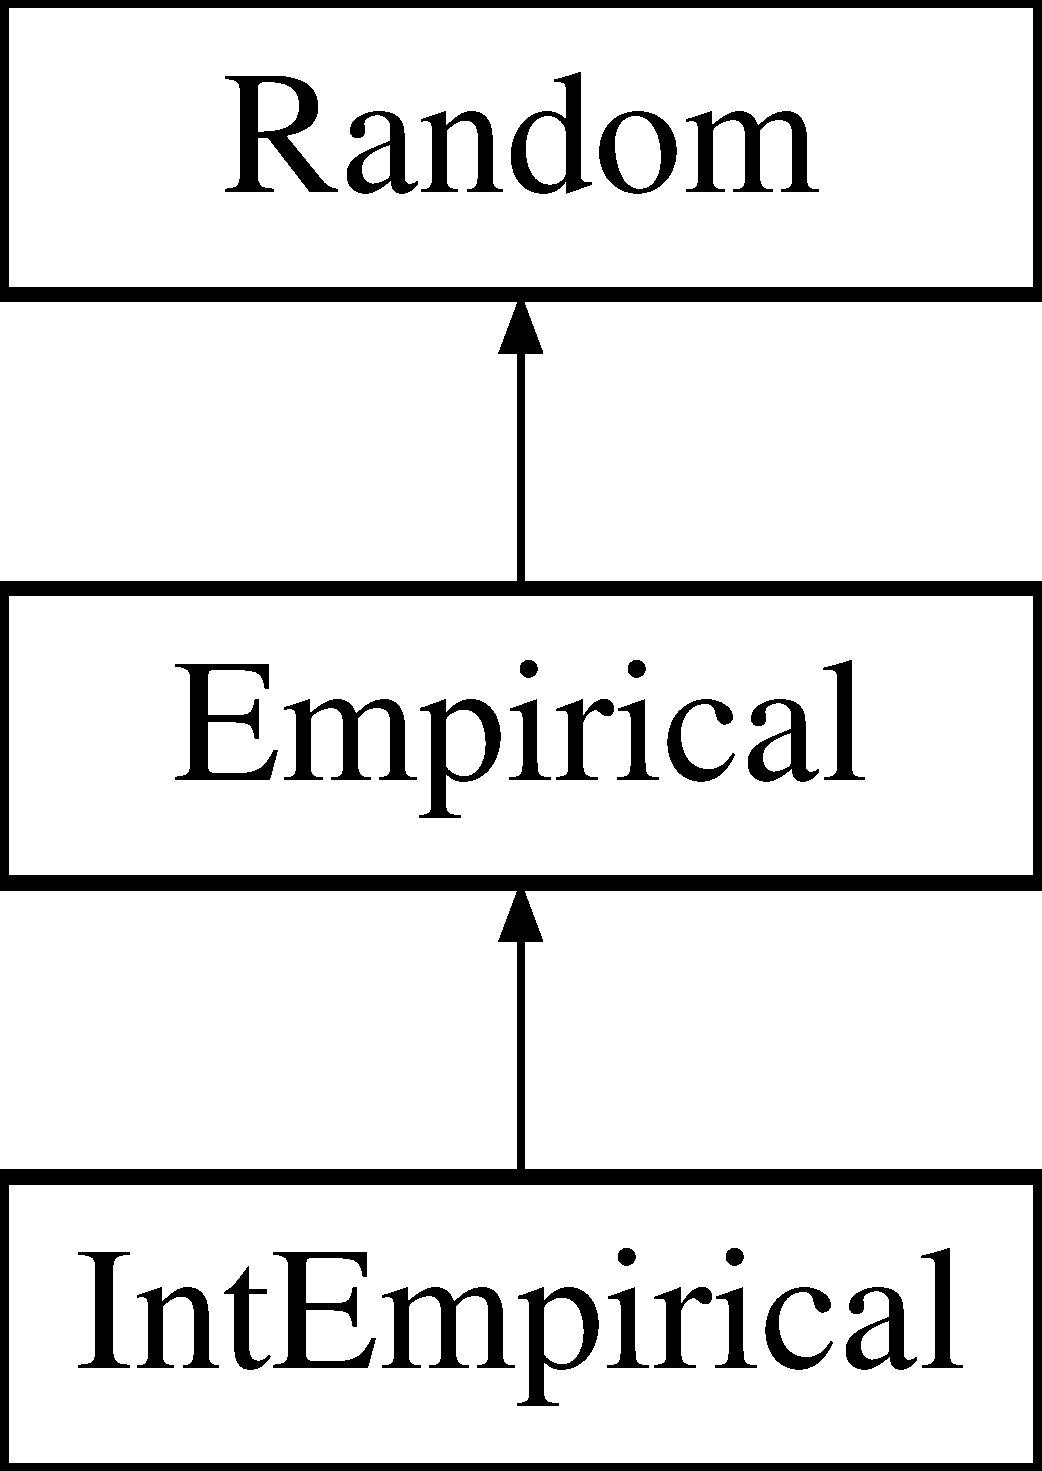
\includegraphics[height=3cm]{classIntEmpirical}
\end{center}
\end{figure}
\subsection*{Public Member Functions}
\begin{CompactItemize}
\item 
\hyperlink{classIntEmpirical_7442c6f9c589166f1d011c794afe9100}{IntEmpirical} ()
\item 
virtual \hyperlink{classRandom}{Random} $\ast$ \hyperlink{classIntEmpirical_d7e809689f9158c050b8a386eb945636}{Copy} () const 
\item 
virtual \hyperlink{rng_8hpp_eb0f2eb55a063defa69eab89c6c0f695}{IRandom\_\-t} \hyperlink{classIntEmpirical_71e5695d2c4b6b6a853cbb2992f81d48}{IntValue} ()
\item 
virtual \hyperlink{rng_8hpp_ad41e7f5d86b1109b6a6a032c86cdd3f}{Random\_\-t} \hyperlink{classIntEmpirical_9137a26418bfb0f912468c034ad1a8e0}{Interpolate} (\hyperlink{rng_8hpp_68ff29d325e1cb493f27ede4fa99c8e4}{CDF\_\-t}, \hyperlink{rng_8hpp_68ff29d325e1cb493f27ede4fa99c8e4}{CDF\_\-t}, \hyperlink{rng_8hpp_ad41e7f5d86b1109b6a6a032c86cdd3f}{Random\_\-t}, \hyperlink{rng_8hpp_ad41e7f5d86b1109b6a6a032c86cdd3f}{Random\_\-t}, \hyperlink{rng_8hpp_68ff29d325e1cb493f27ede4fa99c8e4}{CDF\_\-t})
\end{CompactItemize}


\subsection{Constructor \& Destructor Documentation}
\hypertarget{classIntEmpirical_7442c6f9c589166f1d011c794afe9100}{
\index{IntEmpirical@{IntEmpirical}!IntEmpirical@{IntEmpirical}}
\index{IntEmpirical@{IntEmpirical}!IntEmpirical@{IntEmpirical}}
\subsubsection[{IntEmpirical}]{\setlength{\rightskip}{0pt plus 5cm}IntEmpirical::IntEmpirical ()\hspace{0.3cm}{\tt  \mbox{[}inline\mbox{]}}}}
\label{classIntEmpirical_7442c6f9c589166f1d011c794afe9100}




\subsection{Member Function Documentation}
\hypertarget{classIntEmpirical_d7e809689f9158c050b8a386eb945636}{
\index{IntEmpirical@{IntEmpirical}!Copy@{Copy}}
\index{Copy@{Copy}!IntEmpirical@{IntEmpirical}}
\subsubsection[{Copy}]{\setlength{\rightskip}{0pt plus 5cm}{\bf Random} $\ast$ IntEmpirical::Copy () const\hspace{0.3cm}{\tt  \mbox{[}virtual\mbox{]}}}}
\label{classIntEmpirical_d7e809689f9158c050b8a386eb945636}




Reimplemented from \hyperlink{classEmpirical_d5429fdf863d53d74649cc8c630cfb0b}{Empirical}.\hypertarget{classIntEmpirical_9137a26418bfb0f912468c034ad1a8e0}{
\index{IntEmpirical@{IntEmpirical}!Interpolate@{Interpolate}}
\index{Interpolate@{Interpolate}!IntEmpirical@{IntEmpirical}}
\subsubsection[{Interpolate}]{\setlength{\rightskip}{0pt plus 5cm}{\bf Random\_\-t} IntEmpirical::Interpolate ({\bf CDF\_\-t} {\em c1}, \/  {\bf CDF\_\-t} {\em c2}, \/  {\bf Random\_\-t} {\em v1}, \/  {\bf Random\_\-t} {\em v2}, \/  {\bf CDF\_\-t} {\em r})\hspace{0.3cm}{\tt  \mbox{[}virtual\mbox{]}}}}
\label{classIntEmpirical_9137a26418bfb0f912468c034ad1a8e0}




Reimplemented from \hyperlink{classEmpirical}{Empirical}.\hypertarget{classIntEmpirical_71e5695d2c4b6b6a853cbb2992f81d48}{
\index{IntEmpirical@{IntEmpirical}!IntValue@{IntValue}}
\index{IntValue@{IntValue}!IntEmpirical@{IntEmpirical}}
\subsubsection[{IntValue}]{\setlength{\rightskip}{0pt plus 5cm}{\bf IRandom\_\-t} IntEmpirical::IntValue ()\hspace{0.3cm}{\tt  \mbox{[}virtual\mbox{]}}}}
\label{classIntEmpirical_71e5695d2c4b6b6a853cbb2992f81d48}




Reimplemented from \hyperlink{classRandom_9ac522e9fe39aefd2cddd88554184b1a}{Random}.

The documentation for this class was generated from the following files:\begin{CompactItemize}
\item 
source/randomNumbers/impl/\hyperlink{rng_8hpp}{rng.hpp}\item 
source/randomNumbers/impl/\hyperlink{rng_8cpp}{rng.cpp}\end{CompactItemize}

\hypertarget{classInterface}{
\section{Interface Class Reference}
\label{classInterface}\index{Interface@{Interface}}
}
{\tt \#include $<$interface.h$>$}

Inheritance diagram for Interface::\begin{figure}[H]
\begin{center}
\leavevmode
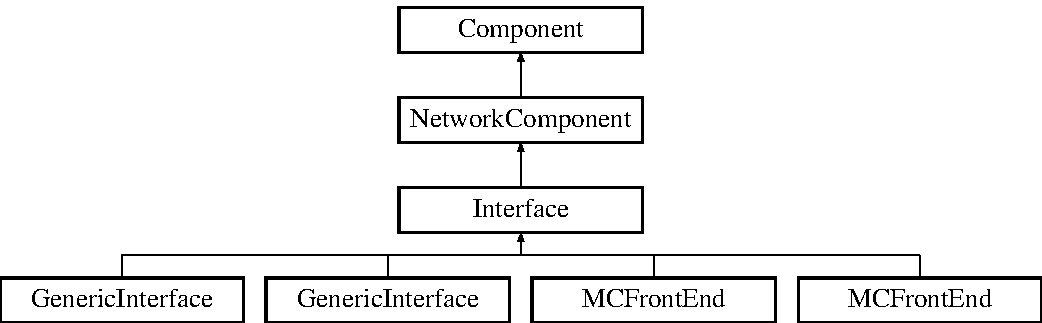
\includegraphics[height=4cm]{classInterface}
\end{center}
\end{figure}
\subsection*{Public Member Functions}
\begin{CompactItemize}
\item 
\hyperlink{classInterface_4406d74c75bdfe150bf72be1f1cda8b1}{Interface} ()
\item 
virtual \hyperlink{classInterface_19179888f29f18f1be54a3dfe98f68c0}{$\sim$Interface} ()
\item 
virtual string \hyperlink{classInterface_137cdb3bca46eb2ae0bbf017d1efb66e}{toString} () const 
\item 
virtual void \hyperlink{classInterface_f9015204e6dabe3e0fce572b19cd1550}{setup} ()=0
\item 
virtual void \hyperlink{classInterface_c458ee6d8e974cb0a9f90308d0feb16d}{set\_\-no\_\-credits} (int cr)=0
\item 
virtual void \hyperlink{classInterface_f2cec7f7aa725d52c8bb02087d7c9e5d}{set\_\-buffer\_\-size} (\hyperlink{outputBuffer_8h_91ad9478d81a7aaf2593e8d9c3d06a14}{uint} cr)=0
\item 
virtual void \hyperlink{classInterface_e7266de6cc9e1dfd4bb3a1b8face3c15}{set\_\-no\_\-vcs} (\hyperlink{outputBuffer_8h_91ad9478d81a7aaf2593e8d9c3d06a14}{uint} cr)=0
\item 
virtual void \hyperlink{classInterface_baaaeb823b1e0fd7ddc1bb32c2f016fb}{process\_\-event} (\hyperlink{classIrisEvent}{IrisEvent} $\ast$e)=0
\item 
virtual string \hyperlink{classInterface_abfe4b675df488fd5a88d2876cff0ebe}{print\_\-stats} ()=0
\end{CompactItemize}
\subsection*{Public Attributes}
\begin{CompactItemize}
\item 
\hyperlink{classNetworkComponent}{NetworkComponent} $\ast$ \hyperlink{classInterface_5008ad5bfdf390821d9b6de2272fbe6d}{processor\_\-connection}
\item 
\hyperlink{classIrisLink}{IrisLink} $\ast$ \hyperlink{classInterface_c14fb826229e323ebef2813f887ac37f}{input\_\-connection}
\item 
\hyperlink{classIrisLink}{IrisLink} $\ast$ \hyperlink{classInterface_2fee13a07ffc4a43dd50892b22feca92}{output\_\-connection}
\end{CompactItemize}


\subsection{Constructor \& Destructor Documentation}
\hypertarget{classInterface_4406d74c75bdfe150bf72be1f1cda8b1}{
\index{Interface@{Interface}!Interface@{Interface}}
\index{Interface@{Interface}!Interface@{Interface}}
\subsubsection[{Interface}]{\setlength{\rightskip}{0pt plus 5cm}Interface::Interface ()}}
\label{classInterface_4406d74c75bdfe150bf72be1f1cda8b1}


\hypertarget{classInterface_19179888f29f18f1be54a3dfe98f68c0}{
\index{Interface@{Interface}!$\sim$Interface@{$\sim$Interface}}
\index{$\sim$Interface@{$\sim$Interface}!Interface@{Interface}}
\subsubsection[{$\sim$Interface}]{\setlength{\rightskip}{0pt plus 5cm}Interface::$\sim$Interface ()\hspace{0.3cm}{\tt  \mbox{[}virtual\mbox{]}}}}
\label{classInterface_19179888f29f18f1be54a3dfe98f68c0}




\subsection{Member Function Documentation}
\hypertarget{classInterface_abfe4b675df488fd5a88d2876cff0ebe}{
\index{Interface@{Interface}!print\_\-stats@{print\_\-stats}}
\index{print\_\-stats@{print\_\-stats}!Interface@{Interface}}
\subsubsection[{print\_\-stats}]{\setlength{\rightskip}{0pt plus 5cm}virtual string Interface::print\_\-stats ()\hspace{0.3cm}{\tt  \mbox{[}pure virtual\mbox{]}}}}
\label{classInterface_abfe4b675df488fd5a88d2876cff0ebe}




Implemented in \hyperlink{classMCFrontEnd_38750cc156a8b88225c58b1c08e4f83e}{MCFrontEnd}, \hyperlink{classGenericInterface_b1be26f08d69932b1ac08094985eb5d6}{GenericInterface}, \hyperlink{classGenericInterface_b1be26f08d69932b1ac08094985eb5d6}{GenericInterface}, and \hyperlink{classMCFrontEnd_38750cc156a8b88225c58b1c08e4f83e}{MCFrontEnd}.\hypertarget{classInterface_baaaeb823b1e0fd7ddc1bb32c2f016fb}{
\index{Interface@{Interface}!process\_\-event@{process\_\-event}}
\index{process\_\-event@{process\_\-event}!Interface@{Interface}}
\subsubsection[{process\_\-event}]{\setlength{\rightskip}{0pt plus 5cm}virtual void Interface::process\_\-event ({\bf IrisEvent} $\ast$ {\em e})\hspace{0.3cm}{\tt  \mbox{[}pure virtual\mbox{]}}}}
\label{classInterface_baaaeb823b1e0fd7ddc1bb32c2f016fb}




Implements \hyperlink{classNetworkComponent_c93793eea1e2d424abe86e110ca8b399}{NetworkComponent}.

Implemented in \hyperlink{classMCFrontEnd_cc935494693a9b02addf8ea8c04f81b3}{MCFrontEnd}, \hyperlink{classGenericInterface_d56b8876204889d3c096fccd61b16b9e}{GenericInterface}, \hyperlink{classGenericInterface_d56b8876204889d3c096fccd61b16b9e}{GenericInterface}, and \hyperlink{classMCFrontEnd_cc935494693a9b02addf8ea8c04f81b3}{MCFrontEnd}.\hypertarget{classInterface_f2cec7f7aa725d52c8bb02087d7c9e5d}{
\index{Interface@{Interface}!set\_\-buffer\_\-size@{set\_\-buffer\_\-size}}
\index{set\_\-buffer\_\-size@{set\_\-buffer\_\-size}!Interface@{Interface}}
\subsubsection[{set\_\-buffer\_\-size}]{\setlength{\rightskip}{0pt plus 5cm}virtual void Interface::set\_\-buffer\_\-size ({\bf uint} {\em cr})\hspace{0.3cm}{\tt  \mbox{[}pure virtual\mbox{]}}}}
\label{classInterface_f2cec7f7aa725d52c8bb02087d7c9e5d}




Implemented in \hyperlink{classGenericInterface_fd1cd1ccd6d355852bee1677cd8b56df}{GenericInterface}, and \hyperlink{classGenericInterface_fd1cd1ccd6d355852bee1677cd8b56df}{GenericInterface}.\hypertarget{classInterface_c458ee6d8e974cb0a9f90308d0feb16d}{
\index{Interface@{Interface}!set\_\-no\_\-credits@{set\_\-no\_\-credits}}
\index{set\_\-no\_\-credits@{set\_\-no\_\-credits}!Interface@{Interface}}
\subsubsection[{set\_\-no\_\-credits}]{\setlength{\rightskip}{0pt plus 5cm}virtual void Interface::set\_\-no\_\-credits (int {\em cr})\hspace{0.3cm}{\tt  \mbox{[}pure virtual\mbox{]}}}}
\label{classInterface_c458ee6d8e974cb0a9f90308d0feb16d}




Implemented in \hyperlink{classGenericInterface_d4d5041bce12cd013a77f476c039c391}{GenericInterface}, and \hyperlink{classGenericInterface_d4d5041bce12cd013a77f476c039c391}{GenericInterface}.\hypertarget{classInterface_e7266de6cc9e1dfd4bb3a1b8face3c15}{
\index{Interface@{Interface}!set\_\-no\_\-vcs@{set\_\-no\_\-vcs}}
\index{set\_\-no\_\-vcs@{set\_\-no\_\-vcs}!Interface@{Interface}}
\subsubsection[{set\_\-no\_\-vcs}]{\setlength{\rightskip}{0pt plus 5cm}virtual void Interface::set\_\-no\_\-vcs ({\bf uint} {\em cr})\hspace{0.3cm}{\tt  \mbox{[}pure virtual\mbox{]}}}}
\label{classInterface_e7266de6cc9e1dfd4bb3a1b8face3c15}




Implemented in \hyperlink{classGenericInterface_10e019a3cafe243d63587656afc5e79f}{GenericInterface}, and \hyperlink{classGenericInterface_10e019a3cafe243d63587656afc5e79f}{GenericInterface}.\hypertarget{classInterface_f9015204e6dabe3e0fce572b19cd1550}{
\index{Interface@{Interface}!setup@{setup}}
\index{setup@{setup}!Interface@{Interface}}
\subsubsection[{setup}]{\setlength{\rightskip}{0pt plus 5cm}virtual void Interface::setup ()\hspace{0.3cm}{\tt  \mbox{[}pure virtual\mbox{]}}}}
\label{classInterface_f9015204e6dabe3e0fce572b19cd1550}




Implemented in \hyperlink{classMCFrontEnd_5f399666cb967c146570e81372fe6be6}{MCFrontEnd}, \hyperlink{classGenericInterface_1aaf2e40e433e913e7ea9cb68693fa7c}{GenericInterface}, \hyperlink{classGenericInterface_1aaf2e40e433e913e7ea9cb68693fa7c}{GenericInterface}, and \hyperlink{classMCFrontEnd_5f399666cb967c146570e81372fe6be6}{MCFrontEnd}.\hypertarget{classInterface_137cdb3bca46eb2ae0bbf017d1efb66e}{
\index{Interface@{Interface}!toString@{toString}}
\index{toString@{toString}!Interface@{Interface}}
\subsubsection[{toString}]{\setlength{\rightskip}{0pt plus 5cm}string Interface::toString () const\hspace{0.3cm}{\tt  \mbox{[}virtual\mbox{]}}}}
\label{classInterface_137cdb3bca46eb2ae0bbf017d1efb66e}




Reimplemented from \hyperlink{classNetworkComponent_9bb9874e1f5705588cb3d9c201d8fc6f}{NetworkComponent}.

Reimplemented in \hyperlink{classMCFrontEnd_9dda980a7ae732e6cb6da7121bc4f539}{MCFrontEnd}, \hyperlink{classGenericInterface_ae1400fce0c7ba48965596ec172e474b}{GenericInterface}, \hyperlink{classGenericInterface_ae1400fce0c7ba48965596ec172e474b}{GenericInterface}, and \hyperlink{classMCFrontEnd_9dda980a7ae732e6cb6da7121bc4f539}{MCFrontEnd}.

\subsection{Member Data Documentation}
\hypertarget{classInterface_c14fb826229e323ebef2813f887ac37f}{
\index{Interface@{Interface}!input\_\-connection@{input\_\-connection}}
\index{input\_\-connection@{input\_\-connection}!Interface@{Interface}}
\subsubsection[{input\_\-connection}]{\setlength{\rightskip}{0pt plus 5cm}{\bf IrisLink}$\ast$ {\bf Interface::input\_\-connection}}}
\label{classInterface_c14fb826229e323ebef2813f887ac37f}


\hypertarget{classInterface_2fee13a07ffc4a43dd50892b22feca92}{
\index{Interface@{Interface}!output\_\-connection@{output\_\-connection}}
\index{output\_\-connection@{output\_\-connection}!Interface@{Interface}}
\subsubsection[{output\_\-connection}]{\setlength{\rightskip}{0pt plus 5cm}{\bf IrisLink}$\ast$ {\bf Interface::output\_\-connection}}}
\label{classInterface_2fee13a07ffc4a43dd50892b22feca92}


\hypertarget{classInterface_5008ad5bfdf390821d9b6de2272fbe6d}{
\index{Interface@{Interface}!processor\_\-connection@{processor\_\-connection}}
\index{processor\_\-connection@{processor\_\-connection}!Interface@{Interface}}
\subsubsection[{processor\_\-connection}]{\setlength{\rightskip}{0pt plus 5cm}{\bf NetworkComponent}$\ast$ {\bf Interface::processor\_\-connection}}}
\label{classInterface_5008ad5bfdf390821d9b6de2272fbe6d}




The documentation for this class was generated from the following files:\begin{CompactItemize}
\item 
source/components/interfaces/\hyperlink{interface_8h}{interface.h}\item 
source/components/interfaces/\hyperlink{interface_8cc}{interface.cc}\end{CompactItemize}

\hypertarget{classIrisEvent}{
\section{IrisEvent Class Reference}
\label{classIrisEvent}\index{IrisEvent@{IrisEvent}}
}
{\tt \#include $<$irisEvent.h$>$}

\subsection*{Public Member Functions}
\begin{CompactItemize}
\item 
\hyperlink{classIrisEvent_231a0a457b0f5469d17804d9ced7cc79}{IrisEvent} ()
\item 
\hyperlink{classIrisEvent_5840e399aa6f659e30dc7757e71dc28b}{$\sim$IrisEvent} ()
\item 
string \hyperlink{classIrisEvent_0af2990076aab1512a61908435010824}{toString} (void)
\end{CompactItemize}
\subsection*{Public Attributes}
\begin{CompactItemize}
\item 
\hyperlink{outputBuffer_8h_91ad9478d81a7aaf2593e8d9c3d06a14}{uint} \hyperlink{classIrisEvent_0ea5ae351f3d7dba0a5ad697a7928754}{src\_\-id}
\item 
\hyperlink{outputBuffer_8h_91ad9478d81a7aaf2593e8d9c3d06a14}{uint} \hyperlink{classIrisEvent_274c046ce64d15b914c0b8cbdebfea31}{dst\_\-id}
\item 
vector$<$ void $\ast$ $>$ \hyperlink{classIrisEvent_26464fd0f931717a1e83b91111efc7b4}{event\_\-data}
\item 
\hyperlink{genericComponentHeader_8h_d88faca783e7aa496cda721d9029a2e3}{simTime} \hyperlink{classIrisEvent_cd8c9add4afdbc69bf7dbcaf8a61ba01}{time}
\item 
\hyperlink{outputBuffer_8h_91ad9478d81a7aaf2593e8d9c3d06a14}{uint} \hyperlink{classIrisEvent_339423ccde297a9d2f4ad3e06fc28030}{type}
\item 
\hyperlink{outputBuffer_8h_91ad9478d81a7aaf2593e8d9c3d06a14}{uint} \hyperlink{classIrisEvent_86ee921447bbc46175221fd912f6e0a7}{vc}
\end{CompactItemize}


\subsection{Constructor \& Destructor Documentation}
\hypertarget{classIrisEvent_231a0a457b0f5469d17804d9ced7cc79}{
\index{IrisEvent@{IrisEvent}!IrisEvent@{IrisEvent}}
\index{IrisEvent@{IrisEvent}!IrisEvent@{IrisEvent}}
\subsubsection[{IrisEvent}]{\setlength{\rightskip}{0pt plus 5cm}IrisEvent::IrisEvent ()}}
\label{classIrisEvent_231a0a457b0f5469d17804d9ced7cc79}


\hypertarget{classIrisEvent_5840e399aa6f659e30dc7757e71dc28b}{
\index{IrisEvent@{IrisEvent}!$\sim$IrisEvent@{$\sim$IrisEvent}}
\index{$\sim$IrisEvent@{$\sim$IrisEvent}!IrisEvent@{IrisEvent}}
\subsubsection[{$\sim$IrisEvent}]{\setlength{\rightskip}{0pt plus 5cm}IrisEvent::$\sim$IrisEvent ()}}
\label{classIrisEvent_5840e399aa6f659e30dc7757e71dc28b}




\subsection{Member Function Documentation}
\hypertarget{classIrisEvent_0af2990076aab1512a61908435010824}{
\index{IrisEvent@{IrisEvent}!toString@{toString}}
\index{toString@{toString}!IrisEvent@{IrisEvent}}
\subsubsection[{toString}]{\setlength{\rightskip}{0pt plus 5cm}string IrisEvent::toString (void)}}
\label{classIrisEvent_0af2990076aab1512a61908435010824}




\subsection{Member Data Documentation}
\hypertarget{classIrisEvent_274c046ce64d15b914c0b8cbdebfea31}{
\index{IrisEvent@{IrisEvent}!dst\_\-id@{dst\_\-id}}
\index{dst\_\-id@{dst\_\-id}!IrisEvent@{IrisEvent}}
\subsubsection[{dst\_\-id}]{\setlength{\rightskip}{0pt plus 5cm}{\bf uint} {\bf IrisEvent::dst\_\-id}}}
\label{classIrisEvent_274c046ce64d15b914c0b8cbdebfea31}


\hypertarget{classIrisEvent_26464fd0f931717a1e83b91111efc7b4}{
\index{IrisEvent@{IrisEvent}!event\_\-data@{event\_\-data}}
\index{event\_\-data@{event\_\-data}!IrisEvent@{IrisEvent}}
\subsubsection[{event\_\-data}]{\setlength{\rightskip}{0pt plus 5cm}vector$<$void $\ast$$>$ {\bf IrisEvent::event\_\-data}}}
\label{classIrisEvent_26464fd0f931717a1e83b91111efc7b4}


\hypertarget{classIrisEvent_0ea5ae351f3d7dba0a5ad697a7928754}{
\index{IrisEvent@{IrisEvent}!src\_\-id@{src\_\-id}}
\index{src\_\-id@{src\_\-id}!IrisEvent@{IrisEvent}}
\subsubsection[{src\_\-id}]{\setlength{\rightskip}{0pt plus 5cm}{\bf uint} {\bf IrisEvent::src\_\-id}}}
\label{classIrisEvent_0ea5ae351f3d7dba0a5ad697a7928754}


\hypertarget{classIrisEvent_cd8c9add4afdbc69bf7dbcaf8a61ba01}{
\index{IrisEvent@{IrisEvent}!time@{time}}
\index{time@{time}!IrisEvent@{IrisEvent}}
\subsubsection[{time}]{\setlength{\rightskip}{0pt plus 5cm}{\bf simTime} {\bf IrisEvent::time}}}
\label{classIrisEvent_cd8c9add4afdbc69bf7dbcaf8a61ba01}


\hypertarget{classIrisEvent_339423ccde297a9d2f4ad3e06fc28030}{
\index{IrisEvent@{IrisEvent}!type@{type}}
\index{type@{type}!IrisEvent@{IrisEvent}}
\subsubsection[{type}]{\setlength{\rightskip}{0pt plus 5cm}{\bf uint} {\bf IrisEvent::type}}}
\label{classIrisEvent_339423ccde297a9d2f4ad3e06fc28030}


\hypertarget{classIrisEvent_86ee921447bbc46175221fd912f6e0a7}{
\index{IrisEvent@{IrisEvent}!vc@{vc}}
\index{vc@{vc}!IrisEvent@{IrisEvent}}
\subsubsection[{vc}]{\setlength{\rightskip}{0pt plus 5cm}{\bf uint} {\bf IrisEvent::vc}}}
\label{classIrisEvent_86ee921447bbc46175221fd912f6e0a7}




The documentation for this class was generated from the following files:\begin{CompactItemize}
\item 
source/data\_\-types/impl/\hyperlink{irisEvent_8h}{irisEvent.h}\item 
source/data\_\-types/impl/\hyperlink{irisEvent_8cc}{irisEvent.cc}\end{CompactItemize}

\hypertarget{classIrisLink}{
\section{IrisLink Class Reference}
\label{classIrisLink}\index{IrisLink@{IrisLink}}
}
{\tt \#include $<$irisLink.h$>$}

Inheritance diagram for IrisLink::\begin{figure}[H]
\begin{center}
\leavevmode
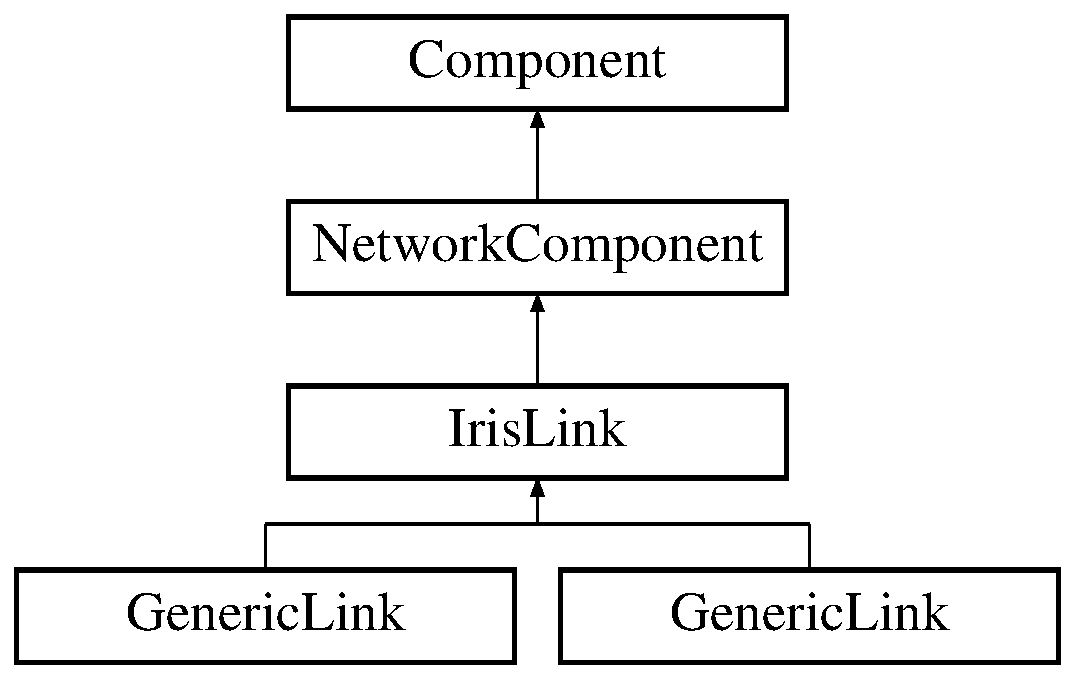
\includegraphics[height=4cm]{classIrisLink}
\end{center}
\end{figure}
\subsection*{Public Member Functions}
\begin{CompactItemize}
\item 
\hyperlink{classIrisLink_338c9fe1f9c8424e885d8e48d43ca2e3}{IrisLink} ()
\item 
\hyperlink{classIrisLink_2d3be414256bdfab31989b0f3c437da2}{$\sim$IrisLink} ()
\item 
string \hyperlink{classIrisLink_d25db1c98385d7abd82180e5746813a6}{toString} () const 
\item 
virtual void \hyperlink{classIrisLink_9c5494bc5716aedf3affe748f3a542c1}{process\_\-event} (\hyperlink{classIrisEvent}{IrisEvent} $\ast$e)=0
\end{CompactItemize}
\subsection*{Public Attributes}
\begin{CompactItemize}
\item 
\hyperlink{classNetworkComponent}{NetworkComponent} $\ast$ \hyperlink{classIrisLink_be439e50b48bbe45bb99c2546f83f9ee}{input\_\-connection}
\item 
\hyperlink{classNetworkComponent}{NetworkComponent} $\ast$ \hyperlink{classIrisLink_137f7502dc308ec2c812753a7ef0b72b}{output\_\-connection}
\end{CompactItemize}


\subsection{Constructor \& Destructor Documentation}
\hypertarget{classIrisLink_338c9fe1f9c8424e885d8e48d43ca2e3}{
\index{IrisLink@{IrisLink}!IrisLink@{IrisLink}}
\index{IrisLink@{IrisLink}!IrisLink@{IrisLink}}
\subsubsection[{IrisLink}]{\setlength{\rightskip}{0pt plus 5cm}IrisLink::IrisLink ()\hspace{0.3cm}{\tt  \mbox{[}inline\mbox{]}}}}
\label{classIrisLink_338c9fe1f9c8424e885d8e48d43ca2e3}


\hypertarget{classIrisLink_2d3be414256bdfab31989b0f3c437da2}{
\index{IrisLink@{IrisLink}!$\sim$IrisLink@{$\sim$IrisLink}}
\index{$\sim$IrisLink@{$\sim$IrisLink}!IrisLink@{IrisLink}}
\subsubsection[{$\sim$IrisLink}]{\setlength{\rightskip}{0pt plus 5cm}IrisLink::$\sim$IrisLink ()\hspace{0.3cm}{\tt  \mbox{[}inline\mbox{]}}}}
\label{classIrisLink_2d3be414256bdfab31989b0f3c437da2}




\subsection{Member Function Documentation}
\hypertarget{classIrisLink_9c5494bc5716aedf3affe748f3a542c1}{
\index{IrisLink@{IrisLink}!process\_\-event@{process\_\-event}}
\index{process\_\-event@{process\_\-event}!IrisLink@{IrisLink}}
\subsubsection[{process\_\-event}]{\setlength{\rightskip}{0pt plus 5cm}virtual void IrisLink::process\_\-event ({\bf IrisEvent} $\ast$ {\em e})\hspace{0.3cm}{\tt  \mbox{[}pure virtual\mbox{]}}}}
\label{classIrisLink_9c5494bc5716aedf3affe748f3a542c1}




Implements \hyperlink{classNetworkComponent_c93793eea1e2d424abe86e110ca8b399}{NetworkComponent}.

Implemented in \hyperlink{classGenericLink_c09533f8445eb3c550c744fd4ada7324}{GenericLink}, and \hyperlink{classGenericLink_c09533f8445eb3c550c744fd4ada7324}{GenericLink}.\hypertarget{classIrisLink_d25db1c98385d7abd82180e5746813a6}{
\index{IrisLink@{IrisLink}!toString@{toString}}
\index{toString@{toString}!IrisLink@{IrisLink}}
\subsubsection[{toString}]{\setlength{\rightskip}{0pt plus 5cm}string IrisLink::toString () const\hspace{0.3cm}{\tt  \mbox{[}virtual\mbox{]}}}}
\label{classIrisLink_d25db1c98385d7abd82180e5746813a6}




Reimplemented from \hyperlink{classNetworkComponent_9bb9874e1f5705588cb3d9c201d8fc6f}{NetworkComponent}.

Reimplemented in \hyperlink{classGenericLink_64dad2c98848fb48b3b572887031167b}{GenericLink}, and \hyperlink{classGenericLink_64dad2c98848fb48b3b572887031167b}{GenericLink}.

\subsection{Member Data Documentation}
\hypertarget{classIrisLink_be439e50b48bbe45bb99c2546f83f9ee}{
\index{IrisLink@{IrisLink}!input\_\-connection@{input\_\-connection}}
\index{input\_\-connection@{input\_\-connection}!IrisLink@{IrisLink}}
\subsubsection[{input\_\-connection}]{\setlength{\rightskip}{0pt plus 5cm}{\bf NetworkComponent}$\ast$ {\bf IrisLink::input\_\-connection}}}
\label{classIrisLink_be439e50b48bbe45bb99c2546f83f9ee}


\hypertarget{classIrisLink_137f7502dc308ec2c812753a7ef0b72b}{
\index{IrisLink@{IrisLink}!output\_\-connection@{output\_\-connection}}
\index{output\_\-connection@{output\_\-connection}!IrisLink@{IrisLink}}
\subsubsection[{output\_\-connection}]{\setlength{\rightskip}{0pt plus 5cm}{\bf NetworkComponent}$\ast$ {\bf IrisLink::output\_\-connection}}}
\label{classIrisLink_137f7502dc308ec2c812753a7ef0b72b}




The documentation for this class was generated from the following files:\begin{CompactItemize}
\item 
source/components/interfaces/\hyperlink{irisLink_8h}{irisLink.h}\item 
source/components/interfaces/\hyperlink{irisLink_8cc}{irisLink.cc}\end{CompactItemize}

\hypertarget{classLink}{
\section{Link Class Reference}
\label{classLink}\index{Link@{Link}}
}
{\tt \#include $<$link.h$>$}

\subsection*{Public Member Functions}
\begin{CompactItemize}
\item 
\hyperlink{classLink_16c40a3222f347d6b3fc2698fc5b9038}{Link} (int srcComponentId, int linkWidth)
\item 
void \hyperlink{classLink_9739f28f141d67a3ab14ddd6e4edc985}{Send} (uint64\_\-t data, int srcComponentId)
\end{CompactItemize}
\subsection*{Public Attributes}
\begin{CompactItemize}
\item 
int \hyperlink{classLink_87fb6a54e52fc0c8cea06eafefc8b555}{src}
\item 
int \hyperlink{classLink_6b5ee52bc53fe5063a5805a8f1a5694f}{width}
\item 
list$<$ \hyperlink{classOutputBase}{OutputBase} $\ast$ $>$ \hyperlink{classLink_ffbc0480926b9f0e59c7581a5ccc1cee}{outputs}
\end{CompactItemize}


\subsection{Constructor \& Destructor Documentation}
\hypertarget{classLink_16c40a3222f347d6b3fc2698fc5b9038}{
\index{Link@{Link}!Link@{Link}}
\index{Link@{Link}!Link@{Link}}
\subsubsection[{Link}]{\setlength{\rightskip}{0pt plus 5cm}Link::Link (int {\em srcComponentId}, \/  int {\em linkWidth})}}
\label{classLink_16c40a3222f347d6b3fc2698fc5b9038}




\subsection{Member Function Documentation}
\hypertarget{classLink_9739f28f141d67a3ab14ddd6e4edc985}{
\index{Link@{Link}!Send@{Send}}
\index{Send@{Send}!Link@{Link}}
\subsubsection[{Send}]{\setlength{\rightskip}{0pt plus 5cm}void Link::Send (uint64\_\-t {\em data}, \/  int {\em srcComponentId})}}
\label{classLink_9739f28f141d67a3ab14ddd6e4edc985}




\subsection{Member Data Documentation}
\hypertarget{classLink_ffbc0480926b9f0e59c7581a5ccc1cee}{
\index{Link@{Link}!outputs@{outputs}}
\index{outputs@{outputs}!Link@{Link}}
\subsubsection[{outputs}]{\setlength{\rightskip}{0pt plus 5cm}list$<${\bf OutputBase}$\ast$$>$ {\bf Link::outputs}}}
\label{classLink_ffbc0480926b9f0e59c7581a5ccc1cee}


\hypertarget{classLink_87fb6a54e52fc0c8cea06eafefc8b555}{
\index{Link@{Link}!src@{src}}
\index{src@{src}!Link@{Link}}
\subsubsection[{src}]{\setlength{\rightskip}{0pt plus 5cm}int {\bf Link::src}}}
\label{classLink_87fb6a54e52fc0c8cea06eafefc8b555}


\hypertarget{classLink_6b5ee52bc53fe5063a5805a8f1a5694f}{
\index{Link@{Link}!width@{width}}
\index{width@{width}!Link@{Link}}
\subsubsection[{width}]{\setlength{\rightskip}{0pt plus 5cm}int {\bf Link::width}}}
\label{classLink_6b5ee52bc53fe5063a5805a8f1a5694f}




The documentation for this class was generated from the following files:\begin{CompactItemize}
\item 
source/kernel/\hyperlink{link_8h}{link.h}\item 
source/kernel/\hyperlink{link_8cc}{link.cc}\end{CompactItemize}

\hypertarget{classLinkArrivalData}{
\section{LinkArrivalData Class Reference}
\label{classLinkArrivalData}\index{LinkArrivalData@{LinkArrivalData}}
}
{\tt \#include $<$genericData.h$>$}

\subsection*{Public Member Functions}
\begin{CompactItemize}
\item 
\hyperlink{classLinkArrivalData_68c73d0d5ad8327bd3d58c82fa5fcef6}{LinkArrivalData} ()
\item 
\hyperlink{classLinkArrivalData_925ca0d6244e409041fd3133efe18ed4}{$\sim$LinkArrivalData} ()
\item 
\hyperlink{classLinkArrivalData_68c73d0d5ad8327bd3d58c82fa5fcef6}{LinkArrivalData} ()
\item 
\hyperlink{classLinkArrivalData_925ca0d6244e409041fd3133efe18ed4}{$\sim$LinkArrivalData} ()
\end{CompactItemize}
\subsection*{Public Attributes}
\begin{CompactItemize}
\item 
\hyperlink{outputBuffer_8h_91ad9478d81a7aaf2593e8d9c3d06a14}{uint} \hyperlink{classLinkArrivalData_67623829975f533c48e4b6552eed2780}{type}
\item 
\hyperlink{outputBuffer_8h_91ad9478d81a7aaf2593e8d9c3d06a14}{uint} \hyperlink{classLinkArrivalData_0015d63ec0989b053ebd3236688d9e9a}{vc}
\item 
\hyperlink{classFlit}{Flit} $\ast$ \hyperlink{classLinkArrivalData_b4f6239cc040642e4020e03bff8a11a2}{ptr}
\item 
bool \hyperlink{classLinkArrivalData_2f9a1f28c8833db08318a1e2b018c9f8}{valid}
\end{CompactItemize}


\subsection{Constructor \& Destructor Documentation}
\hypertarget{classLinkArrivalData_68c73d0d5ad8327bd3d58c82fa5fcef6}{
\index{LinkArrivalData@{LinkArrivalData}!LinkArrivalData@{LinkArrivalData}}
\index{LinkArrivalData@{LinkArrivalData}!LinkArrivalData@{LinkArrivalData}}
\subsubsection[{LinkArrivalData}]{\setlength{\rightskip}{0pt plus 5cm}LinkArrivalData::LinkArrivalData ()}}
\label{classLinkArrivalData_68c73d0d5ad8327bd3d58c82fa5fcef6}


\hypertarget{classLinkArrivalData_925ca0d6244e409041fd3133efe18ed4}{
\index{LinkArrivalData@{LinkArrivalData}!$\sim$LinkArrivalData@{$\sim$LinkArrivalData}}
\index{$\sim$LinkArrivalData@{$\sim$LinkArrivalData}!LinkArrivalData@{LinkArrivalData}}
\subsubsection[{$\sim$LinkArrivalData}]{\setlength{\rightskip}{0pt plus 5cm}LinkArrivalData::$\sim$LinkArrivalData ()}}
\label{classLinkArrivalData_925ca0d6244e409041fd3133efe18ed4}


\hypertarget{classLinkArrivalData_68c73d0d5ad8327bd3d58c82fa5fcef6}{
\index{LinkArrivalData@{LinkArrivalData}!LinkArrivalData@{LinkArrivalData}}
\index{LinkArrivalData@{LinkArrivalData}!LinkArrivalData@{LinkArrivalData}}
\subsubsection[{LinkArrivalData}]{\setlength{\rightskip}{0pt plus 5cm}LinkArrivalData::LinkArrivalData ()}}
\label{classLinkArrivalData_68c73d0d5ad8327bd3d58c82fa5fcef6}


\hypertarget{classLinkArrivalData_925ca0d6244e409041fd3133efe18ed4}{
\index{LinkArrivalData@{LinkArrivalData}!$\sim$LinkArrivalData@{$\sim$LinkArrivalData}}
\index{$\sim$LinkArrivalData@{$\sim$LinkArrivalData}!LinkArrivalData@{LinkArrivalData}}
\subsubsection[{$\sim$LinkArrivalData}]{\setlength{\rightskip}{0pt plus 5cm}LinkArrivalData::$\sim$LinkArrivalData ()}}
\label{classLinkArrivalData_925ca0d6244e409041fd3133efe18ed4}




\subsection{Member Data Documentation}
\hypertarget{classLinkArrivalData_b4f6239cc040642e4020e03bff8a11a2}{
\index{LinkArrivalData@{LinkArrivalData}!ptr@{ptr}}
\index{ptr@{ptr}!LinkArrivalData@{LinkArrivalData}}
\subsubsection[{ptr}]{\setlength{\rightskip}{0pt plus 5cm}{\bf Flit} $\ast$ {\bf LinkArrivalData::ptr}}}
\label{classLinkArrivalData_b4f6239cc040642e4020e03bff8a11a2}


\hypertarget{classLinkArrivalData_67623829975f533c48e4b6552eed2780}{
\index{LinkArrivalData@{LinkArrivalData}!type@{type}}
\index{type@{type}!LinkArrivalData@{LinkArrivalData}}
\subsubsection[{type}]{\setlength{\rightskip}{0pt plus 5cm}{\bf uint} {\bf LinkArrivalData::type}}}
\label{classLinkArrivalData_67623829975f533c48e4b6552eed2780}


\hypertarget{classLinkArrivalData_2f9a1f28c8833db08318a1e2b018c9f8}{
\index{LinkArrivalData@{LinkArrivalData}!valid@{valid}}
\index{valid@{valid}!LinkArrivalData@{LinkArrivalData}}
\subsubsection[{valid}]{\setlength{\rightskip}{0pt plus 5cm}bool {\bf LinkArrivalData::valid}}}
\label{classLinkArrivalData_2f9a1f28c8833db08318a1e2b018c9f8}


\hypertarget{classLinkArrivalData_0015d63ec0989b053ebd3236688d9e9a}{
\index{LinkArrivalData@{LinkArrivalData}!vc@{vc}}
\index{vc@{vc}!LinkArrivalData@{LinkArrivalData}}
\subsubsection[{vc}]{\setlength{\rightskip}{0pt plus 5cm}{\bf uint} {\bf LinkArrivalData::vc}}}
\label{classLinkArrivalData_0015d63ec0989b053ebd3236688d9e9a}




The documentation for this class was generated from the following files:\begin{CompactItemize}
\item 
source/components/impl/\hyperlink{impl_2genericData_8h}{genericData.h}\item 
source/components/none/\hyperlink{none_2genericData_8h}{genericData.h}\item 
source/components/impl/\hyperlink{impl_2genericData_8cc}{genericData.cc}\item 
source/components/none/\hyperlink{none_2genericData_8cc}{genericData.cc}\end{CompactItemize}

\hypertarget{classLowLevelPacket}{
\section{LowLevelPacket Class Reference}
\label{classLowLevelPacket}\index{LowLevelPacket@{LowLevelPacket}}
}
{\tt \#include $<$lowLevelPacket.h$>$}

\subsection*{Public Member Functions}
\begin{CompactItemize}
\item 
\hyperlink{classLowLevelPacket_550561f33ccae00163b40e963121c156}{LowLevelPacket} ()
\item 
\hyperlink{classLowLevelPacket_52d6041c394872c42cd4211e09ca76d4}{$\sim$LowLevelPacket} ()
\item 
void \hyperlink{classLowLevelPacket_726a1d04c62dc4f20de1bcd7bebd031d}{clear} ()
\item 
void \hyperlink{classLowLevelPacket_b2d005a02fb4645db9145f699d330656}{add} (\hyperlink{classFlit}{Flit} $\ast$ptr)
\item 
\hyperlink{classFlit}{Flit} $\ast$ \hyperlink{classLowLevelPacket_01bcea53e1afb4be73ddaa8503e053dc}{at} (\hyperlink{outputBuffer_8h_91ad9478d81a7aaf2593e8d9c3d06a14}{uint} index)
\item 
\hyperlink{classFlit}{Flit} $\ast$ \hyperlink{classLowLevelPacket_508b439358881368b5ef646ef36b4cac}{get\_\-next\_\-flit} ()
\item 
string \hyperlink{classLowLevelPacket_5a52563bae0560cb9b0b9a6d44adde6c}{toString} () const 
\item 
bool \hyperlink{classLowLevelPacket_1053348a061e1878e90a4f49d383889f}{valid\_\-packet} ()
\item 
\hyperlink{outputBuffer_8h_91ad9478d81a7aaf2593e8d9c3d06a14}{uint} \hyperlink{classLowLevelPacket_f61b1051a4dbda237dbeb1bd74220d20}{size} ()
\item 
void \hyperlink{classLowLevelPacket_5a52c8b9499a757227a71ba51f1ef61a}{operator=} (const \hyperlink{classLowLevelPacket}{LowLevelPacket} $\ast$p)
\end{CompactItemize}
\subsection*{Public Attributes}
\begin{CompactItemize}
\item 
deque$<$ \hyperlink{classFlit}{Flit} $\ast$ $>$ \hyperlink{classLowLevelPacket_eee86f15c92fad6be8b7e6bc4df223e3}{flits}
\item 
\hyperlink{outputBuffer_8h_91ad9478d81a7aaf2593e8d9c3d06a14}{uint} \hyperlink{classLowLevelPacket_c7aee6df6db0e4bb8e5be36b061a95bc}{source}
\item 
\hyperlink{outputBuffer_8h_91ad9478d81a7aaf2593e8d9c3d06a14}{uint} \hyperlink{classLowLevelPacket_225808b46aefe4d252c040e91c9411b0}{destination}
\item 
\hyperlink{outputBuffer_8h_91ad9478d81a7aaf2593e8d9c3d06a14}{uint} \hyperlink{classLowLevelPacket_ed8dd9d70bac87be59a61fe8ac4b399d}{transaction\_\-id}
\item 
short int \hyperlink{classLowLevelPacket_3fa4ac5563bbf3005a809c0b193f4c84}{virtual\_\-channel}
\item 
unsigned long int \hyperlink{classLowLevelPacket_8a51892863d89c8b8b28f75c19fa0199}{sent\_\-time}
\item 
unsigned int \hyperlink{classLowLevelPacket_69297a63b62cdce301d004782cc3ef3c}{length}
\item 
vector$<$ bool $>$ \hyperlink{classLowLevelPacket_7537b9b0339e77d3d4a2d04998e1a950}{control\_\-bits}
\end{CompactItemize}


\subsection{Constructor \& Destructor Documentation}
\hypertarget{classLowLevelPacket_550561f33ccae00163b40e963121c156}{
\index{LowLevelPacket@{LowLevelPacket}!LowLevelPacket@{LowLevelPacket}}
\index{LowLevelPacket@{LowLevelPacket}!LowLevelPacket@{LowLevelPacket}}
\subsubsection[{LowLevelPacket}]{\setlength{\rightskip}{0pt plus 5cm}LowLevelPacket::LowLevelPacket ()}}
\label{classLowLevelPacket_550561f33ccae00163b40e963121c156}


\hypertarget{classLowLevelPacket_52d6041c394872c42cd4211e09ca76d4}{
\index{LowLevelPacket@{LowLevelPacket}!$\sim$LowLevelPacket@{$\sim$LowLevelPacket}}
\index{$\sim$LowLevelPacket@{$\sim$LowLevelPacket}!LowLevelPacket@{LowLevelPacket}}
\subsubsection[{$\sim$LowLevelPacket}]{\setlength{\rightskip}{0pt plus 5cm}LowLevelPacket::$\sim$LowLevelPacket ()}}
\label{classLowLevelPacket_52d6041c394872c42cd4211e09ca76d4}




\subsection{Member Function Documentation}
\hypertarget{classLowLevelPacket_b2d005a02fb4645db9145f699d330656}{
\index{LowLevelPacket@{LowLevelPacket}!add@{add}}
\index{add@{add}!LowLevelPacket@{LowLevelPacket}}
\subsubsection[{add}]{\setlength{\rightskip}{0pt plus 5cm}void LowLevelPacket::add ({\bf Flit} $\ast$ {\em ptr})}}
\label{classLowLevelPacket_b2d005a02fb4645db9145f699d330656}


\hypertarget{classLowLevelPacket_01bcea53e1afb4be73ddaa8503e053dc}{
\index{LowLevelPacket@{LowLevelPacket}!at@{at}}
\index{at@{at}!LowLevelPacket@{LowLevelPacket}}
\subsubsection[{at}]{\setlength{\rightskip}{0pt plus 5cm}{\bf Flit} $\ast$ LowLevelPacket::at ({\bf uint} {\em index})}}
\label{classLowLevelPacket_01bcea53e1afb4be73ddaa8503e053dc}


\hypertarget{classLowLevelPacket_726a1d04c62dc4f20de1bcd7bebd031d}{
\index{LowLevelPacket@{LowLevelPacket}!clear@{clear}}
\index{clear@{clear}!LowLevelPacket@{LowLevelPacket}}
\subsubsection[{clear}]{\setlength{\rightskip}{0pt plus 5cm}void LowLevelPacket::clear ()}}
\label{classLowLevelPacket_726a1d04c62dc4f20de1bcd7bebd031d}


\hypertarget{classLowLevelPacket_508b439358881368b5ef646ef36b4cac}{
\index{LowLevelPacket@{LowLevelPacket}!get\_\-next\_\-flit@{get\_\-next\_\-flit}}
\index{get\_\-next\_\-flit@{get\_\-next\_\-flit}!LowLevelPacket@{LowLevelPacket}}
\subsubsection[{get\_\-next\_\-flit}]{\setlength{\rightskip}{0pt plus 5cm}{\bf Flit} $\ast$ LowLevelPacket::get\_\-next\_\-flit ()}}
\label{classLowLevelPacket_508b439358881368b5ef646ef36b4cac}


\hypertarget{classLowLevelPacket_5a52c8b9499a757227a71ba51f1ef61a}{
\index{LowLevelPacket@{LowLevelPacket}!operator=@{operator=}}
\index{operator=@{operator=}!LowLevelPacket@{LowLevelPacket}}
\subsubsection[{operator=}]{\setlength{\rightskip}{0pt plus 5cm}void LowLevelPacket::operator= (const {\bf LowLevelPacket} $\ast$ {\em p})}}
\label{classLowLevelPacket_5a52c8b9499a757227a71ba51f1ef61a}


\hypertarget{classLowLevelPacket_f61b1051a4dbda237dbeb1bd74220d20}{
\index{LowLevelPacket@{LowLevelPacket}!size@{size}}
\index{size@{size}!LowLevelPacket@{LowLevelPacket}}
\subsubsection[{size}]{\setlength{\rightskip}{0pt plus 5cm}{\bf uint} LowLevelPacket::size ()}}
\label{classLowLevelPacket_f61b1051a4dbda237dbeb1bd74220d20}


\hypertarget{classLowLevelPacket_5a52563bae0560cb9b0b9a6d44adde6c}{
\index{LowLevelPacket@{LowLevelPacket}!toString@{toString}}
\index{toString@{toString}!LowLevelPacket@{LowLevelPacket}}
\subsubsection[{toString}]{\setlength{\rightskip}{0pt plus 5cm}string LowLevelPacket::toString (void) const}}
\label{classLowLevelPacket_5a52563bae0560cb9b0b9a6d44adde6c}


\hypertarget{classLowLevelPacket_1053348a061e1878e90a4f49d383889f}{
\index{LowLevelPacket@{LowLevelPacket}!valid\_\-packet@{valid\_\-packet}}
\index{valid\_\-packet@{valid\_\-packet}!LowLevelPacket@{LowLevelPacket}}
\subsubsection[{valid\_\-packet}]{\setlength{\rightskip}{0pt plus 5cm}bool LowLevelPacket::valid\_\-packet ()}}
\label{classLowLevelPacket_1053348a061e1878e90a4f49d383889f}




\subsection{Member Data Documentation}
\hypertarget{classLowLevelPacket_7537b9b0339e77d3d4a2d04998e1a950}{
\index{LowLevelPacket@{LowLevelPacket}!control\_\-bits@{control\_\-bits}}
\index{control\_\-bits@{control\_\-bits}!LowLevelPacket@{LowLevelPacket}}
\subsubsection[{control\_\-bits}]{\setlength{\rightskip}{0pt plus 5cm}vector$<$bool$>$ {\bf LowLevelPacket::control\_\-bits}}}
\label{classLowLevelPacket_7537b9b0339e77d3d4a2d04998e1a950}


\hypertarget{classLowLevelPacket_225808b46aefe4d252c040e91c9411b0}{
\index{LowLevelPacket@{LowLevelPacket}!destination@{destination}}
\index{destination@{destination}!LowLevelPacket@{LowLevelPacket}}
\subsubsection[{destination}]{\setlength{\rightskip}{0pt plus 5cm}{\bf uint} {\bf LowLevelPacket::destination}}}
\label{classLowLevelPacket_225808b46aefe4d252c040e91c9411b0}


\hypertarget{classLowLevelPacket_eee86f15c92fad6be8b7e6bc4df223e3}{
\index{LowLevelPacket@{LowLevelPacket}!flits@{flits}}
\index{flits@{flits}!LowLevelPacket@{LowLevelPacket}}
\subsubsection[{flits}]{\setlength{\rightskip}{0pt plus 5cm}deque$<${\bf Flit}$\ast$$>$ {\bf LowLevelPacket::flits}}}
\label{classLowLevelPacket_eee86f15c92fad6be8b7e6bc4df223e3}


\hypertarget{classLowLevelPacket_69297a63b62cdce301d004782cc3ef3c}{
\index{LowLevelPacket@{LowLevelPacket}!length@{length}}
\index{length@{length}!LowLevelPacket@{LowLevelPacket}}
\subsubsection[{length}]{\setlength{\rightskip}{0pt plus 5cm}unsigned int {\bf LowLevelPacket::length}}}
\label{classLowLevelPacket_69297a63b62cdce301d004782cc3ef3c}


\hypertarget{classLowLevelPacket_8a51892863d89c8b8b28f75c19fa0199}{
\index{LowLevelPacket@{LowLevelPacket}!sent\_\-time@{sent\_\-time}}
\index{sent\_\-time@{sent\_\-time}!LowLevelPacket@{LowLevelPacket}}
\subsubsection[{sent\_\-time}]{\setlength{\rightskip}{0pt plus 5cm}unsigned long int {\bf LowLevelPacket::sent\_\-time}}}
\label{classLowLevelPacket_8a51892863d89c8b8b28f75c19fa0199}


\hypertarget{classLowLevelPacket_c7aee6df6db0e4bb8e5be36b061a95bc}{
\index{LowLevelPacket@{LowLevelPacket}!source@{source}}
\index{source@{source}!LowLevelPacket@{LowLevelPacket}}
\subsubsection[{source}]{\setlength{\rightskip}{0pt plus 5cm}{\bf uint} {\bf LowLevelPacket::source}}}
\label{classLowLevelPacket_c7aee6df6db0e4bb8e5be36b061a95bc}


\hypertarget{classLowLevelPacket_ed8dd9d70bac87be59a61fe8ac4b399d}{
\index{LowLevelPacket@{LowLevelPacket}!transaction\_\-id@{transaction\_\-id}}
\index{transaction\_\-id@{transaction\_\-id}!LowLevelPacket@{LowLevelPacket}}
\subsubsection[{transaction\_\-id}]{\setlength{\rightskip}{0pt plus 5cm}{\bf uint} {\bf LowLevelPacket::transaction\_\-id}}}
\label{classLowLevelPacket_ed8dd9d70bac87be59a61fe8ac4b399d}


\hypertarget{classLowLevelPacket_3fa4ac5563bbf3005a809c0b193f4c84}{
\index{LowLevelPacket@{LowLevelPacket}!virtual\_\-channel@{virtual\_\-channel}}
\index{virtual\_\-channel@{virtual\_\-channel}!LowLevelPacket@{LowLevelPacket}}
\subsubsection[{virtual\_\-channel}]{\setlength{\rightskip}{0pt plus 5cm}short int {\bf LowLevelPacket::virtual\_\-channel}}}
\label{classLowLevelPacket_3fa4ac5563bbf3005a809c0b193f4c84}




The documentation for this class was generated from the following files:\begin{CompactItemize}
\item 
source/data\_\-types/impl/\hyperlink{lowLevelPacket_8h}{lowLevelPacket.h}\item 
source/data\_\-types/impl/\hyperlink{lowLevelPacket_8cc}{lowLevelPacket.cc}\end{CompactItemize}

\hypertarget{classMCFrontEnd}{
\section{MCFrontEnd Class Reference}
\label{classMCFrontEnd}\index{MCFrontEnd@{MCFrontEnd}}
}
{\tt \#include $<$mcFrontEnd.h$>$}

Inheritance diagram for MCFrontEnd::\begin{figure}[H]
\begin{center}
\leavevmode
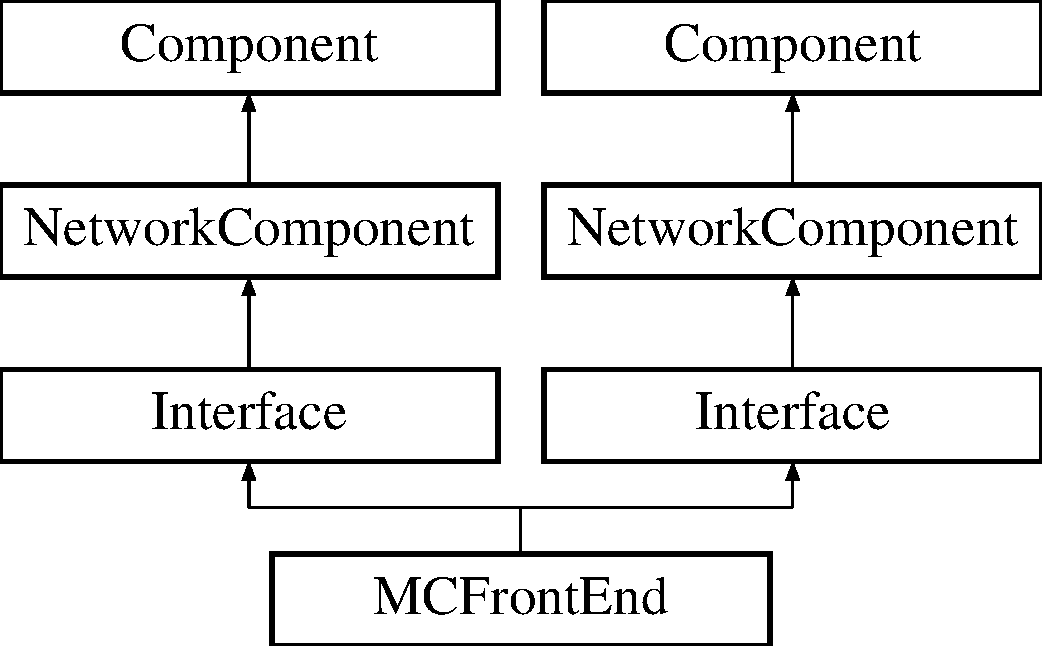
\includegraphics[height=4cm]{classMCFrontEnd}
\end{center}
\end{figure}
\subsection*{Public Member Functions}
\begin{CompactItemize}
\item 
\hyperlink{classMCFrontEnd_26241509c8a72b46cf6ff3b843601b63}{MCFrontEnd} ()
\item 
\hyperlink{classMCFrontEnd_a6661a18919e7ef025ff32c955243b5d}{$\sim$MCFrontEnd} ()
\item 
void \hyperlink{classMCFrontEnd_5f399666cb967c146570e81372fe6be6}{setup} ()
\item 
\hyperlink{outputBuffer_8h_91ad9478d81a7aaf2593e8d9c3d06a14}{uint} \hyperlink{classMCFrontEnd_9db80e378e0c7255bf66d43e2350cc15}{get\_\-no\_\-credits} () const 
\item 
void \hyperlink{classMCFrontEnd_eb0cc4a818d1a8dd1cdc071da8519628}{set\_\-no\_\-credits} (\hyperlink{outputBuffer_8h_91ad9478d81a7aaf2593e8d9c3d06a14}{uint} credits)
\item 
string \hyperlink{classMCFrontEnd_9dda980a7ae732e6cb6da7121bc4f539}{toString} () const 
\item 
string \hyperlink{classMCFrontEnd_38750cc156a8b88225c58b1c08e4f83e}{print\_\-stats} ()
\item 
void \hyperlink{classMCFrontEnd_cc935494693a9b02addf8ea8c04f81b3}{process\_\-event} (\hyperlink{classIrisEvent}{IrisEvent} $\ast$e)
\item 
\hyperlink{classMCFrontEnd_26241509c8a72b46cf6ff3b843601b63}{MCFrontEnd} ()
\item 
\hyperlink{classMCFrontEnd_a6661a18919e7ef025ff32c955243b5d}{$\sim$MCFrontEnd} ()
\item 
void \hyperlink{classMCFrontEnd_5f399666cb967c146570e81372fe6be6}{setup} ()
\item 
\hyperlink{outputBuffer_8h_91ad9478d81a7aaf2593e8d9c3d06a14}{uint} \hyperlink{classMCFrontEnd_9db80e378e0c7255bf66d43e2350cc15}{get\_\-no\_\-credits} () const 
\item 
void \hyperlink{classMCFrontEnd_eb0cc4a818d1a8dd1cdc071da8519628}{set\_\-no\_\-credits} (\hyperlink{outputBuffer_8h_91ad9478d81a7aaf2593e8d9c3d06a14}{uint} credits)
\item 
string \hyperlink{classMCFrontEnd_9dda980a7ae732e6cb6da7121bc4f539}{toString} () const 
\item 
string \hyperlink{classMCFrontEnd_38750cc156a8b88225c58b1c08e4f83e}{print\_\-stats} ()
\item 
void \hyperlink{classMCFrontEnd_cc935494693a9b02addf8ea8c04f81b3}{process\_\-event} (\hyperlink{classIrisEvent}{IrisEvent} $\ast$e)
\end{CompactItemize}
\subsection*{Public Attributes}
\begin{CompactItemize}
\item 
\hyperlink{outputBuffer_8h_91ad9478d81a7aaf2593e8d9c3d06a14}{uint} \hyperlink{classMCFrontEnd_99eed4a2a554a84018c06637e863b525}{node\_\-ip}
\item 
\hyperlink{classGenericOutputBuffer}{GenericOutputBuffer} \hyperlink{classMCFrontEnd_573d6ed88ea7603b71f29c8d09995997}{out\_\-buffer}
\item 
\hyperlink{classGenericArbiter}{GenericArbiter} \hyperlink{classMCFrontEnd_8a05a43c211013595ed1e81ade65c58a}{out\_\-arbiter}
\item 
\hyperlink{classGenericArbiter}{GenericArbiter} \hyperlink{classMCFrontEnd_366abfbae09ca49371a4c5ea5548820d}{in\_\-arbiter}
\item 
\hyperlink{classGenericOutputBuffer}{GenericOutputBuffer} \hyperlink{classMCFrontEnd_7f312b013c788e1d28ac936d8808795e}{in\_\-buffer}
\end{CompactItemize}


\subsection{Constructor \& Destructor Documentation}
\hypertarget{classMCFrontEnd_26241509c8a72b46cf6ff3b843601b63}{
\index{MCFrontEnd@{MCFrontEnd}!MCFrontEnd@{MCFrontEnd}}
\index{MCFrontEnd@{MCFrontEnd}!MCFrontEnd@{MCFrontEnd}}
\subsubsection[{MCFrontEnd}]{\setlength{\rightskip}{0pt plus 5cm}MCFrontEnd::MCFrontEnd ()}}
\label{classMCFrontEnd_26241509c8a72b46cf6ff3b843601b63}


\hypertarget{classMCFrontEnd_a6661a18919e7ef025ff32c955243b5d}{
\index{MCFrontEnd@{MCFrontEnd}!$\sim$MCFrontEnd@{$\sim$MCFrontEnd}}
\index{$\sim$MCFrontEnd@{$\sim$MCFrontEnd}!MCFrontEnd@{MCFrontEnd}}
\subsubsection[{$\sim$MCFrontEnd}]{\setlength{\rightskip}{0pt plus 5cm}MCFrontEnd::$\sim$MCFrontEnd ()}}
\label{classMCFrontEnd_a6661a18919e7ef025ff32c955243b5d}


\hypertarget{classMCFrontEnd_26241509c8a72b46cf6ff3b843601b63}{
\index{MCFrontEnd@{MCFrontEnd}!MCFrontEnd@{MCFrontEnd}}
\index{MCFrontEnd@{MCFrontEnd}!MCFrontEnd@{MCFrontEnd}}
\subsubsection[{MCFrontEnd}]{\setlength{\rightskip}{0pt plus 5cm}MCFrontEnd::MCFrontEnd ()}}
\label{classMCFrontEnd_26241509c8a72b46cf6ff3b843601b63}


\hypertarget{classMCFrontEnd_a6661a18919e7ef025ff32c955243b5d}{
\index{MCFrontEnd@{MCFrontEnd}!$\sim$MCFrontEnd@{$\sim$MCFrontEnd}}
\index{$\sim$MCFrontEnd@{$\sim$MCFrontEnd}!MCFrontEnd@{MCFrontEnd}}
\subsubsection[{$\sim$MCFrontEnd}]{\setlength{\rightskip}{0pt plus 5cm}MCFrontEnd::$\sim$MCFrontEnd ()}}
\label{classMCFrontEnd_a6661a18919e7ef025ff32c955243b5d}




\subsection{Member Function Documentation}
\hypertarget{classMCFrontEnd_9db80e378e0c7255bf66d43e2350cc15}{
\index{MCFrontEnd@{MCFrontEnd}!get\_\-no\_\-credits@{get\_\-no\_\-credits}}
\index{get\_\-no\_\-credits@{get\_\-no\_\-credits}!MCFrontEnd@{MCFrontEnd}}
\subsubsection[{get\_\-no\_\-credits}]{\setlength{\rightskip}{0pt plus 5cm}{\bf uint} MCFrontEnd::get\_\-no\_\-credits () const}}
\label{classMCFrontEnd_9db80e378e0c7255bf66d43e2350cc15}


\hypertarget{classMCFrontEnd_9db80e378e0c7255bf66d43e2350cc15}{
\index{MCFrontEnd@{MCFrontEnd}!get\_\-no\_\-credits@{get\_\-no\_\-credits}}
\index{get\_\-no\_\-credits@{get\_\-no\_\-credits}!MCFrontEnd@{MCFrontEnd}}
\subsubsection[{get\_\-no\_\-credits}]{\setlength{\rightskip}{0pt plus 5cm}{\bf uint} MCFrontEnd::get\_\-no\_\-credits () const}}
\label{classMCFrontEnd_9db80e378e0c7255bf66d43e2350cc15}


\hypertarget{classMCFrontEnd_38750cc156a8b88225c58b1c08e4f83e}{
\index{MCFrontEnd@{MCFrontEnd}!print\_\-stats@{print\_\-stats}}
\index{print\_\-stats@{print\_\-stats}!MCFrontEnd@{MCFrontEnd}}
\subsubsection[{print\_\-stats}]{\setlength{\rightskip}{0pt plus 5cm}string MCFrontEnd::print\_\-stats ()\hspace{0.3cm}{\tt  \mbox{[}virtual\mbox{]}}}}
\label{classMCFrontEnd_38750cc156a8b88225c58b1c08e4f83e}




Implements \hyperlink{classInterface_abfe4b675df488fd5a88d2876cff0ebe}{Interface}.\hypertarget{classMCFrontEnd_38750cc156a8b88225c58b1c08e4f83e}{
\index{MCFrontEnd@{MCFrontEnd}!print\_\-stats@{print\_\-stats}}
\index{print\_\-stats@{print\_\-stats}!MCFrontEnd@{MCFrontEnd}}
\subsubsection[{print\_\-stats}]{\setlength{\rightskip}{0pt plus 5cm}string MCFrontEnd::print\_\-stats ()\hspace{0.3cm}{\tt  \mbox{[}virtual\mbox{]}}}}
\label{classMCFrontEnd_38750cc156a8b88225c58b1c08e4f83e}




Implements \hyperlink{classInterface_abfe4b675df488fd5a88d2876cff0ebe}{Interface}.\hypertarget{classMCFrontEnd_cc935494693a9b02addf8ea8c04f81b3}{
\index{MCFrontEnd@{MCFrontEnd}!process\_\-event@{process\_\-event}}
\index{process\_\-event@{process\_\-event}!MCFrontEnd@{MCFrontEnd}}
\subsubsection[{process\_\-event}]{\setlength{\rightskip}{0pt plus 5cm}void MCFrontEnd::process\_\-event ({\bf IrisEvent} $\ast$ {\em e})\hspace{0.3cm}{\tt  \mbox{[}virtual\mbox{]}}}}
\label{classMCFrontEnd_cc935494693a9b02addf8ea8c04f81b3}




Implements \hyperlink{classInterface_baaaeb823b1e0fd7ddc1bb32c2f016fb}{Interface}.\hypertarget{classMCFrontEnd_cc935494693a9b02addf8ea8c04f81b3}{
\index{MCFrontEnd@{MCFrontEnd}!process\_\-event@{process\_\-event}}
\index{process\_\-event@{process\_\-event}!MCFrontEnd@{MCFrontEnd}}
\subsubsection[{process\_\-event}]{\setlength{\rightskip}{0pt plus 5cm}void MCFrontEnd::process\_\-event ({\bf IrisEvent} $\ast$ {\em e})\hspace{0.3cm}{\tt  \mbox{[}virtual\mbox{]}}}}
\label{classMCFrontEnd_cc935494693a9b02addf8ea8c04f81b3}




Implements \hyperlink{classInterface_baaaeb823b1e0fd7ddc1bb32c2f016fb}{Interface}.\hypertarget{classMCFrontEnd_eb0cc4a818d1a8dd1cdc071da8519628}{
\index{MCFrontEnd@{MCFrontEnd}!set\_\-no\_\-credits@{set\_\-no\_\-credits}}
\index{set\_\-no\_\-credits@{set\_\-no\_\-credits}!MCFrontEnd@{MCFrontEnd}}
\subsubsection[{set\_\-no\_\-credits}]{\setlength{\rightskip}{0pt plus 5cm}void MCFrontEnd::set\_\-no\_\-credits ({\bf uint} {\em credits})}}
\label{classMCFrontEnd_eb0cc4a818d1a8dd1cdc071da8519628}


\hypertarget{classMCFrontEnd_eb0cc4a818d1a8dd1cdc071da8519628}{
\index{MCFrontEnd@{MCFrontEnd}!set\_\-no\_\-credits@{set\_\-no\_\-credits}}
\index{set\_\-no\_\-credits@{set\_\-no\_\-credits}!MCFrontEnd@{MCFrontEnd}}
\subsubsection[{set\_\-no\_\-credits}]{\setlength{\rightskip}{0pt plus 5cm}void MCFrontEnd::set\_\-no\_\-credits ({\bf uint} {\em credits})}}
\label{classMCFrontEnd_eb0cc4a818d1a8dd1cdc071da8519628}


\hypertarget{classMCFrontEnd_5f399666cb967c146570e81372fe6be6}{
\index{MCFrontEnd@{MCFrontEnd}!setup@{setup}}
\index{setup@{setup}!MCFrontEnd@{MCFrontEnd}}
\subsubsection[{setup}]{\setlength{\rightskip}{0pt plus 5cm}void MCFrontEnd::setup ()\hspace{0.3cm}{\tt  \mbox{[}virtual\mbox{]}}}}
\label{classMCFrontEnd_5f399666cb967c146570e81372fe6be6}




Implements \hyperlink{classInterface_f9015204e6dabe3e0fce572b19cd1550}{Interface}.\hypertarget{classMCFrontEnd_5f399666cb967c146570e81372fe6be6}{
\index{MCFrontEnd@{MCFrontEnd}!setup@{setup}}
\index{setup@{setup}!MCFrontEnd@{MCFrontEnd}}
\subsubsection[{setup}]{\setlength{\rightskip}{0pt plus 5cm}void MCFrontEnd::setup ()\hspace{0.3cm}{\tt  \mbox{[}virtual\mbox{]}}}}
\label{classMCFrontEnd_5f399666cb967c146570e81372fe6be6}




Implements \hyperlink{classInterface_f9015204e6dabe3e0fce572b19cd1550}{Interface}.\hypertarget{classMCFrontEnd_9dda980a7ae732e6cb6da7121bc4f539}{
\index{MCFrontEnd@{MCFrontEnd}!toString@{toString}}
\index{toString@{toString}!MCFrontEnd@{MCFrontEnd}}
\subsubsection[{toString}]{\setlength{\rightskip}{0pt plus 5cm}string MCFrontEnd::toString () const\hspace{0.3cm}{\tt  \mbox{[}virtual\mbox{]}}}}
\label{classMCFrontEnd_9dda980a7ae732e6cb6da7121bc4f539}




Reimplemented from \hyperlink{classInterface_137cdb3bca46eb2ae0bbf017d1efb66e}{Interface}.\hypertarget{classMCFrontEnd_9dda980a7ae732e6cb6da7121bc4f539}{
\index{MCFrontEnd@{MCFrontEnd}!toString@{toString}}
\index{toString@{toString}!MCFrontEnd@{MCFrontEnd}}
\subsubsection[{toString}]{\setlength{\rightskip}{0pt plus 5cm}string MCFrontEnd::toString () const\hspace{0.3cm}{\tt  \mbox{[}virtual\mbox{]}}}}
\label{classMCFrontEnd_9dda980a7ae732e6cb6da7121bc4f539}




Reimplemented from \hyperlink{classInterface_137cdb3bca46eb2ae0bbf017d1efb66e}{Interface}.

\subsection{Member Data Documentation}
\hypertarget{classMCFrontEnd_366abfbae09ca49371a4c5ea5548820d}{
\index{MCFrontEnd@{MCFrontEnd}!in\_\-arbiter@{in\_\-arbiter}}
\index{in\_\-arbiter@{in\_\-arbiter}!MCFrontEnd@{MCFrontEnd}}
\subsubsection[{in\_\-arbiter}]{\setlength{\rightskip}{0pt plus 5cm}{\bf GenericArbiter} {\bf MCFrontEnd::in\_\-arbiter}}}
\label{classMCFrontEnd_366abfbae09ca49371a4c5ea5548820d}


\hypertarget{classMCFrontEnd_7f312b013c788e1d28ac936d8808795e}{
\index{MCFrontEnd@{MCFrontEnd}!in\_\-buffer@{in\_\-buffer}}
\index{in\_\-buffer@{in\_\-buffer}!MCFrontEnd@{MCFrontEnd}}
\subsubsection[{in\_\-buffer}]{\setlength{\rightskip}{0pt plus 5cm}{\bf GenericOutputBuffer} {\bf MCFrontEnd::in\_\-buffer}}}
\label{classMCFrontEnd_7f312b013c788e1d28ac936d8808795e}


\hypertarget{classMCFrontEnd_99eed4a2a554a84018c06637e863b525}{
\index{MCFrontEnd@{MCFrontEnd}!node\_\-ip@{node\_\-ip}}
\index{node\_\-ip@{node\_\-ip}!MCFrontEnd@{MCFrontEnd}}
\subsubsection[{node\_\-ip}]{\setlength{\rightskip}{0pt plus 5cm}{\bf uint} {\bf MCFrontEnd::node\_\-ip}}}
\label{classMCFrontEnd_99eed4a2a554a84018c06637e863b525}




Reimplemented from \hyperlink{classNetworkComponent_56599b3484333fb78af1b6c33f77cf16}{NetworkComponent}.\hypertarget{classMCFrontEnd_8a05a43c211013595ed1e81ade65c58a}{
\index{MCFrontEnd@{MCFrontEnd}!out\_\-arbiter@{out\_\-arbiter}}
\index{out\_\-arbiter@{out\_\-arbiter}!MCFrontEnd@{MCFrontEnd}}
\subsubsection[{out\_\-arbiter}]{\setlength{\rightskip}{0pt plus 5cm}{\bf GenericArbiter} {\bf MCFrontEnd::out\_\-arbiter}}}
\label{classMCFrontEnd_8a05a43c211013595ed1e81ade65c58a}


\hypertarget{classMCFrontEnd_573d6ed88ea7603b71f29c8d09995997}{
\index{MCFrontEnd@{MCFrontEnd}!out\_\-buffer@{out\_\-buffer}}
\index{out\_\-buffer@{out\_\-buffer}!MCFrontEnd@{MCFrontEnd}}
\subsubsection[{out\_\-buffer}]{\setlength{\rightskip}{0pt plus 5cm}{\bf GenericOutputBuffer} {\bf MCFrontEnd::out\_\-buffer}}}
\label{classMCFrontEnd_573d6ed88ea7603b71f29c8d09995997}




The documentation for this class was generated from the following files:\begin{CompactItemize}
\item 
source/components/impl/backup/\hyperlink{impl_2backup_2mcFrontEnd_8h}{mcFrontEnd.h}\item 
source/components/none/\hyperlink{none_2mcFrontEnd_8h}{mcFrontEnd.h}\item 
source/components/impl/backup/\hyperlink{impl_2backup_2mcFrontEnd_8cc}{mcFrontEnd.cc}\item 
source/components/none/\hyperlink{none_2mcFrontEnd_8cc}{mcFrontEnd.cc}\end{CompactItemize}

\hypertarget{classMesh}{
\section{Mesh Class Reference}
\label{classMesh}\index{Mesh@{Mesh}}
}
{\tt \#include $<$mesh.h$>$}

\subsection*{Public Member Functions}
\begin{CompactItemize}
\item 
\hyperlink{classMesh_2af137f1571af89172b9c102302c416b}{Mesh} ()
\item 
\hyperlink{classMesh_5efe4da1a4c0971cfb037bd70304c303}{$\sim$Mesh} ()
\item 
void \hyperlink{classMesh_678dc93df5115714b2d2e9a5932692db}{init} (\hyperlink{outputBuffer_8h_91ad9478d81a7aaf2593e8d9c3d06a14}{uint} ports, \hyperlink{outputBuffer_8h_91ad9478d81a7aaf2593e8d9c3d06a14}{uint} vcs, \hyperlink{outputBuffer_8h_91ad9478d81a7aaf2593e8d9c3d06a14}{uint} credits, \hyperlink{outputBuffer_8h_91ad9478d81a7aaf2593e8d9c3d06a14}{uint} buffer\_\-size, \hyperlink{outputBuffer_8h_91ad9478d81a7aaf2593e8d9c3d06a14}{uint} no\_\-nodes, \hyperlink{outputBuffer_8h_91ad9478d81a7aaf2593e8d9c3d06a14}{uint} grid\_\-size, \hyperlink{outputBuffer_8h_91ad9478d81a7aaf2593e8d9c3d06a14}{uint} links)
\item 
void \hyperlink{classMesh_5c83ba3ef93b8ab63084b9c45082c7e9}{setup} (void)
\item 
void \hyperlink{classMesh_9dfad9769d936905f5d8b0e4ffad6743}{connect\_\-interface\_\-processor} (void)
\item 
void \hyperlink{classMesh_0bee0b7a3c9b621524748a97a3575db7}{connect\_\-interface\_\-routers} (void)
\item 
void \hyperlink{classMesh_fea2e233774ea469b02cff87afc336bc}{connect\_\-routers} (void)
\item 
string \hyperlink{classMesh_eea84429f858784c6232e5633603fdf8}{print\_\-stats} (void)
\end{CompactItemize}
\subsection*{Public Attributes}
\begin{CompactItemize}
\item 
vector$<$ \hyperlink{classRouter}{Router} $\ast$ $>$ \hyperlink{classMesh_da66e4e75f4e50237af30d495248cca2}{routers}
\item 
vector$<$ \hyperlink{classInterface}{Interface} $\ast$ $>$ \hyperlink{classMesh_9ebde4264da1ba6e8f24bd2a24d05ef8}{interfaces}
\item 
vector$<$ \hyperlink{classProcessor}{Processor} $\ast$ $>$ \hyperlink{classMesh_e3531860febe9e7194b5d44ac1c1b2d8}{processors}
\item 
vector$<$ \hyperlink{classGenericLink}{GenericLink} $\ast$ $>$ \hyperlink{classMesh_25aed9e44396cd39a521e647d8e95ed2}{link\_\-a}
\item 
vector$<$ \hyperlink{classGenericLink}{GenericLink} $\ast$ $>$ \hyperlink{classMesh_8afcc482b97d3820e8249750c8a214c2}{link\_\-b}
\end{CompactItemize}


\subsection{Constructor \& Destructor Documentation}
\hypertarget{classMesh_2af137f1571af89172b9c102302c416b}{
\index{Mesh@{Mesh}!Mesh@{Mesh}}
\index{Mesh@{Mesh}!Mesh@{Mesh}}
\subsubsection[{Mesh}]{\setlength{\rightskip}{0pt plus 5cm}Mesh::Mesh ()}}
\label{classMesh_2af137f1571af89172b9c102302c416b}


\hypertarget{classMesh_5efe4da1a4c0971cfb037bd70304c303}{
\index{Mesh@{Mesh}!$\sim$Mesh@{$\sim$Mesh}}
\index{$\sim$Mesh@{$\sim$Mesh}!Mesh@{Mesh}}
\subsubsection[{$\sim$Mesh}]{\setlength{\rightskip}{0pt plus 5cm}Mesh::$\sim$Mesh ()}}
\label{classMesh_5efe4da1a4c0971cfb037bd70304c303}




\subsection{Member Function Documentation}
\hypertarget{classMesh_9dfad9769d936905f5d8b0e4ffad6743}{
\index{Mesh@{Mesh}!connect\_\-interface\_\-processor@{connect\_\-interface\_\-processor}}
\index{connect\_\-interface\_\-processor@{connect\_\-interface\_\-processor}!Mesh@{Mesh}}
\subsubsection[{connect\_\-interface\_\-processor}]{\setlength{\rightskip}{0pt plus 5cm}void Mesh::connect\_\-interface\_\-processor (void)}}
\label{classMesh_9dfad9769d936905f5d8b0e4ffad6743}


\hypertarget{classMesh_0bee0b7a3c9b621524748a97a3575db7}{
\index{Mesh@{Mesh}!connect\_\-interface\_\-routers@{connect\_\-interface\_\-routers}}
\index{connect\_\-interface\_\-routers@{connect\_\-interface\_\-routers}!Mesh@{Mesh}}
\subsubsection[{connect\_\-interface\_\-routers}]{\setlength{\rightskip}{0pt plus 5cm}void Mesh::connect\_\-interface\_\-routers (void)}}
\label{classMesh_0bee0b7a3c9b621524748a97a3575db7}


\hypertarget{classMesh_fea2e233774ea469b02cff87afc336bc}{
\index{Mesh@{Mesh}!connect\_\-routers@{connect\_\-routers}}
\index{connect\_\-routers@{connect\_\-routers}!Mesh@{Mesh}}
\subsubsection[{connect\_\-routers}]{\setlength{\rightskip}{0pt plus 5cm}void Mesh::connect\_\-routers (void)}}
\label{classMesh_fea2e233774ea469b02cff87afc336bc}


\hypertarget{classMesh_678dc93df5115714b2d2e9a5932692db}{
\index{Mesh@{Mesh}!init@{init}}
\index{init@{init}!Mesh@{Mesh}}
\subsubsection[{init}]{\setlength{\rightskip}{0pt plus 5cm}void Mesh::init ({\bf uint} {\em ports}, \/  {\bf uint} {\em vcs}, \/  {\bf uint} {\em credits}, \/  {\bf uint} {\em buffer\_\-size}, \/  {\bf uint} {\em no\_\-nodes}, \/  {\bf uint} {\em grid\_\-size}, \/  {\bf uint} {\em links})}}
\label{classMesh_678dc93df5115714b2d2e9a5932692db}


\hypertarget{classMesh_eea84429f858784c6232e5633603fdf8}{
\index{Mesh@{Mesh}!print\_\-stats@{print\_\-stats}}
\index{print\_\-stats@{print\_\-stats}!Mesh@{Mesh}}
\subsubsection[{print\_\-stats}]{\setlength{\rightskip}{0pt plus 5cm}string Mesh::print\_\-stats (void)}}
\label{classMesh_eea84429f858784c6232e5633603fdf8}


\hypertarget{classMesh_5c83ba3ef93b8ab63084b9c45082c7e9}{
\index{Mesh@{Mesh}!setup@{setup}}
\index{setup@{setup}!Mesh@{Mesh}}
\subsubsection[{setup}]{\setlength{\rightskip}{0pt plus 5cm}void Mesh::setup (void)}}
\label{classMesh_5c83ba3ef93b8ab63084b9c45082c7e9}




\subsection{Member Data Documentation}
\hypertarget{classMesh_9ebde4264da1ba6e8f24bd2a24d05ef8}{
\index{Mesh@{Mesh}!interfaces@{interfaces}}
\index{interfaces@{interfaces}!Mesh@{Mesh}}
\subsubsection[{interfaces}]{\setlength{\rightskip}{0pt plus 5cm}vector$<${\bf Interface}$\ast$$>$ {\bf Mesh::interfaces}}}
\label{classMesh_9ebde4264da1ba6e8f24bd2a24d05ef8}


\hypertarget{classMesh_25aed9e44396cd39a521e647d8e95ed2}{
\index{Mesh@{Mesh}!link\_\-a@{link\_\-a}}
\index{link\_\-a@{link\_\-a}!Mesh@{Mesh}}
\subsubsection[{link\_\-a}]{\setlength{\rightskip}{0pt plus 5cm}vector$<${\bf GenericLink}$\ast$$>$ {\bf Mesh::link\_\-a}}}
\label{classMesh_25aed9e44396cd39a521e647d8e95ed2}


\hypertarget{classMesh_8afcc482b97d3820e8249750c8a214c2}{
\index{Mesh@{Mesh}!link\_\-b@{link\_\-b}}
\index{link\_\-b@{link\_\-b}!Mesh@{Mesh}}
\subsubsection[{link\_\-b}]{\setlength{\rightskip}{0pt plus 5cm}vector$<${\bf GenericLink}$\ast$$>$ {\bf Mesh::link\_\-b}}}
\label{classMesh_8afcc482b97d3820e8249750c8a214c2}


\hypertarget{classMesh_e3531860febe9e7194b5d44ac1c1b2d8}{
\index{Mesh@{Mesh}!processors@{processors}}
\index{processors@{processors}!Mesh@{Mesh}}
\subsubsection[{processors}]{\setlength{\rightskip}{0pt plus 5cm}vector$<${\bf Processor}$\ast$$>$ {\bf Mesh::processors}}}
\label{classMesh_e3531860febe9e7194b5d44ac1c1b2d8}


\hypertarget{classMesh_da66e4e75f4e50237af30d495248cca2}{
\index{Mesh@{Mesh}!routers@{routers}}
\index{routers@{routers}!Mesh@{Mesh}}
\subsubsection[{routers}]{\setlength{\rightskip}{0pt plus 5cm}vector$<${\bf Router}$\ast$$>$ {\bf Mesh::routers}}}
\label{classMesh_da66e4e75f4e50237af30d495248cca2}




The documentation for this class was generated from the following files:\begin{CompactItemize}
\item 
source/frontend/impl/\hyperlink{mesh_8h}{mesh.h}\item 
source/frontend/impl/\hyperlink{mesh_8cc}{mesh.cc}\end{CompactItemize}

\hypertarget{classMessageState}{
\section{MessageState Class Reference}
\label{classMessageState}\index{MessageState@{MessageState}}
}
{\tt \#include $<$genericRouterNoVcs.h$>$}

\subsection*{Public Member Functions}
\begin{CompactItemize}
\item 
\hyperlink{classMessageState_ad9003377a5ab63ece9eedd35bae105e}{MessageState} ()
\item 
\hyperlink{classMessageState_5ad0eb922535da32b91d990e64843ec2}{$\sim$MessageState} ()
\item 
string \hyperlink{classMessageState_16ae858ec7ab2042f10cb92f1f4dbd7a}{toString} () const 
\item 
\hyperlink{classMessageState_ad9003377a5ab63ece9eedd35bae105e}{MessageState} ()
\item 
\hyperlink{classMessageState_5ad0eb922535da32b91d990e64843ec2}{$\sim$MessageState} ()
\item 
string \hyperlink{classMessageState_16ae858ec7ab2042f10cb92f1f4dbd7a}{toString} () const 
\item 
\hyperlink{classMessageState_ad9003377a5ab63ece9eedd35bae105e}{MessageState} ()
\item 
\hyperlink{classMessageState_5ad0eb922535da32b91d990e64843ec2}{$\sim$MessageState} ()
\item 
string \hyperlink{classMessageState_16ae858ec7ab2042f10cb92f1f4dbd7a}{toString} () const 
\end{CompactItemize}
\subsection*{Public Attributes}
\begin{CompactItemize}
\item 
\hyperlink{outputBuffer_8h_91ad9478d81a7aaf2593e8d9c3d06a14}{uint} \hyperlink{classMessageState_e559b3e67832d9dadfa22e4d1e881f66}{input\_\-port}
\item 
\hyperlink{outputBuffer_8h_91ad9478d81a7aaf2593e8d9c3d06a14}{uint} \hyperlink{classMessageState_c3aa8bd6020f05968251f82ecc513e73}{input\_\-channel}
\item 
\hyperlink{outputBuffer_8h_91ad9478d81a7aaf2593e8d9c3d06a14}{uint} \hyperlink{classMessageState_c2c10a29b3f589757b00648e886d656b}{output\_\-port}
\item 
\hyperlink{outputBuffer_8h_91ad9478d81a7aaf2593e8d9c3d06a14}{uint} \hyperlink{classMessageState_504a771d0ecbe3c1a8abb105ce3d24b8}{output\_\-channel}
\item 
double \hyperlink{classMessageState_a0e6516b0f5557c9ab36172cebc34483}{arrival\_\-time}
\item 
int \hyperlink{classMessageState_d42d02c6268b0f589c411a328df27741}{length}
\item 
int \hyperlink{classMessageState_dc0b600f04abf68ec43182d229030f2e}{credits\_\-sent}
\item 
vector$<$ \hyperlink{outputBuffer_8h_91ad9478d81a7aaf2593e8d9c3d06a14}{uint} $>$ \hyperlink{classMessageState_d21e16291161c6a70e4a962a71c5b3d0}{possible\_\-ovcs}
\item 
vector$<$ \hyperlink{outputBuffer_8h_91ad9478d81a7aaf2593e8d9c3d06a14}{uint} $>$ \hyperlink{classMessageState_377d4cf5d0d42ac641e9ca890e9276b0}{possible\_\-oports}
\item 
\hyperlink{backup_2genericRouterNoVcs_8h_0cff66db447a0cf3554d6c28ab84b579}{GenericRouterNoVcsPipeStage} \hyperlink{classMessageState_d4cb410d4a081d6e2f7b79c49298d905}{pipe\_\-stage}
\item 
bool \hyperlink{classMessageState_3e912089a01660c7082eaf19102d72f7}{clear\_\-message}
\item 
\hyperlink{outputBuffer_8h_91ad9478d81a7aaf2593e8d9c3d06a14}{uint} \hyperlink{classMessageState_4885fe36f0608415df17504b09e869e6}{flits\_\-in\_\-ib}
\item 
\hyperlink{myRouter_8h_ffc4ec97b4c53d9d256d3b4ea2f58ac8}{MyRouterPipeStage} \hyperlink{classMessageState_4ebb2bdcb326ffa6ecf9edfd5ea4d577}{pipe\_\-stage}
\end{CompactItemize}


\subsection{Constructor \& Destructor Documentation}
\hypertarget{classMessageState_ad9003377a5ab63ece9eedd35bae105e}{
\index{MessageState@{MessageState}!MessageState@{MessageState}}
\index{MessageState@{MessageState}!MessageState@{MessageState}}
\subsubsection[{MessageState}]{\setlength{\rightskip}{0pt plus 5cm}MessageState::MessageState ()}}
\label{classMessageState_ad9003377a5ab63ece9eedd35bae105e}


\hypertarget{classMessageState_5ad0eb922535da32b91d990e64843ec2}{
\index{MessageState@{MessageState}!$\sim$MessageState@{$\sim$MessageState}}
\index{$\sim$MessageState@{$\sim$MessageState}!MessageState@{MessageState}}
\subsubsection[{$\sim$MessageState}]{\setlength{\rightskip}{0pt plus 5cm}MessageState::$\sim$MessageState ()\hspace{0.3cm}{\tt  \mbox{[}inline\mbox{]}}}}
\label{classMessageState_5ad0eb922535da32b91d990e64843ec2}


\hypertarget{classMessageState_ad9003377a5ab63ece9eedd35bae105e}{
\index{MessageState@{MessageState}!MessageState@{MessageState}}
\index{MessageState@{MessageState}!MessageState@{MessageState}}
\subsubsection[{MessageState}]{\setlength{\rightskip}{0pt plus 5cm}MessageState::MessageState ()}}
\label{classMessageState_ad9003377a5ab63ece9eedd35bae105e}


\hypertarget{classMessageState_5ad0eb922535da32b91d990e64843ec2}{
\index{MessageState@{MessageState}!$\sim$MessageState@{$\sim$MessageState}}
\index{$\sim$MessageState@{$\sim$MessageState}!MessageState@{MessageState}}
\subsubsection[{$\sim$MessageState}]{\setlength{\rightskip}{0pt plus 5cm}MessageState::$\sim$MessageState ()\hspace{0.3cm}{\tt  \mbox{[}inline\mbox{]}}}}
\label{classMessageState_5ad0eb922535da32b91d990e64843ec2}


\hypertarget{classMessageState_ad9003377a5ab63ece9eedd35bae105e}{
\index{MessageState@{MessageState}!MessageState@{MessageState}}
\index{MessageState@{MessageState}!MessageState@{MessageState}}
\subsubsection[{MessageState}]{\setlength{\rightskip}{0pt plus 5cm}MessageState::MessageState ()}}
\label{classMessageState_ad9003377a5ab63ece9eedd35bae105e}


\hypertarget{classMessageState_5ad0eb922535da32b91d990e64843ec2}{
\index{MessageState@{MessageState}!$\sim$MessageState@{$\sim$MessageState}}
\index{$\sim$MessageState@{$\sim$MessageState}!MessageState@{MessageState}}
\subsubsection[{$\sim$MessageState}]{\setlength{\rightskip}{0pt plus 5cm}MessageState::$\sim$MessageState ()\hspace{0.3cm}{\tt  \mbox{[}inline\mbox{]}}}}
\label{classMessageState_5ad0eb922535da32b91d990e64843ec2}




\subsection{Member Function Documentation}
\hypertarget{classMessageState_16ae858ec7ab2042f10cb92f1f4dbd7a}{
\index{MessageState@{MessageState}!toString@{toString}}
\index{toString@{toString}!MessageState@{MessageState}}
\subsubsection[{toString}]{\setlength{\rightskip}{0pt plus 5cm}string MessageState::toString () const}}
\label{classMessageState_16ae858ec7ab2042f10cb92f1f4dbd7a}


\hypertarget{classMessageState_16ae858ec7ab2042f10cb92f1f4dbd7a}{
\index{MessageState@{MessageState}!toString@{toString}}
\index{toString@{toString}!MessageState@{MessageState}}
\subsubsection[{toString}]{\setlength{\rightskip}{0pt plus 5cm}string MessageState::toString () const}}
\label{classMessageState_16ae858ec7ab2042f10cb92f1f4dbd7a}


\hypertarget{classMessageState_16ae858ec7ab2042f10cb92f1f4dbd7a}{
\index{MessageState@{MessageState}!toString@{toString}}
\index{toString@{toString}!MessageState@{MessageState}}
\subsubsection[{toString}]{\setlength{\rightskip}{0pt plus 5cm}string MessageState::toString () const}}
\label{classMessageState_16ae858ec7ab2042f10cb92f1f4dbd7a}




\subsection{Member Data Documentation}
\hypertarget{classMessageState_a0e6516b0f5557c9ab36172cebc34483}{
\index{MessageState@{MessageState}!arrival\_\-time@{arrival\_\-time}}
\index{arrival\_\-time@{arrival\_\-time}!MessageState@{MessageState}}
\subsubsection[{arrival\_\-time}]{\setlength{\rightskip}{0pt plus 5cm}double {\bf MessageState::arrival\_\-time}}}
\label{classMessageState_a0e6516b0f5557c9ab36172cebc34483}


\hypertarget{classMessageState_3e912089a01660c7082eaf19102d72f7}{
\index{MessageState@{MessageState}!clear\_\-message@{clear\_\-message}}
\index{clear\_\-message@{clear\_\-message}!MessageState@{MessageState}}
\subsubsection[{clear\_\-message}]{\setlength{\rightskip}{0pt plus 5cm}bool {\bf MessageState::clear\_\-message}}}
\label{classMessageState_3e912089a01660c7082eaf19102d72f7}


\hypertarget{classMessageState_dc0b600f04abf68ec43182d229030f2e}{
\index{MessageState@{MessageState}!credits\_\-sent@{credits\_\-sent}}
\index{credits\_\-sent@{credits\_\-sent}!MessageState@{MessageState}}
\subsubsection[{credits\_\-sent}]{\setlength{\rightskip}{0pt plus 5cm}int {\bf MessageState::credits\_\-sent}}}
\label{classMessageState_dc0b600f04abf68ec43182d229030f2e}


\hypertarget{classMessageState_4885fe36f0608415df17504b09e869e6}{
\index{MessageState@{MessageState}!flits\_\-in\_\-ib@{flits\_\-in\_\-ib}}
\index{flits\_\-in\_\-ib@{flits\_\-in\_\-ib}!MessageState@{MessageState}}
\subsubsection[{flits\_\-in\_\-ib}]{\setlength{\rightskip}{0pt plus 5cm}{\bf uint} {\bf MessageState::flits\_\-in\_\-ib}}}
\label{classMessageState_4885fe36f0608415df17504b09e869e6}


\hypertarget{classMessageState_c3aa8bd6020f05968251f82ecc513e73}{
\index{MessageState@{MessageState}!input\_\-channel@{input\_\-channel}}
\index{input\_\-channel@{input\_\-channel}!MessageState@{MessageState}}
\subsubsection[{input\_\-channel}]{\setlength{\rightskip}{0pt plus 5cm}{\bf uint} {\bf MessageState::input\_\-channel}}}
\label{classMessageState_c3aa8bd6020f05968251f82ecc513e73}


\hypertarget{classMessageState_e559b3e67832d9dadfa22e4d1e881f66}{
\index{MessageState@{MessageState}!input\_\-port@{input\_\-port}}
\index{input\_\-port@{input\_\-port}!MessageState@{MessageState}}
\subsubsection[{input\_\-port}]{\setlength{\rightskip}{0pt plus 5cm}{\bf uint} {\bf MessageState::input\_\-port}}}
\label{classMessageState_e559b3e67832d9dadfa22e4d1e881f66}


\hypertarget{classMessageState_d42d02c6268b0f589c411a328df27741}{
\index{MessageState@{MessageState}!length@{length}}
\index{length@{length}!MessageState@{MessageState}}
\subsubsection[{length}]{\setlength{\rightskip}{0pt plus 5cm}int {\bf MessageState::length}}}
\label{classMessageState_d42d02c6268b0f589c411a328df27741}


\hypertarget{classMessageState_504a771d0ecbe3c1a8abb105ce3d24b8}{
\index{MessageState@{MessageState}!output\_\-channel@{output\_\-channel}}
\index{output\_\-channel@{output\_\-channel}!MessageState@{MessageState}}
\subsubsection[{output\_\-channel}]{\setlength{\rightskip}{0pt plus 5cm}{\bf uint} {\bf MessageState::output\_\-channel}}}
\label{classMessageState_504a771d0ecbe3c1a8abb105ce3d24b8}


\hypertarget{classMessageState_c2c10a29b3f589757b00648e886d656b}{
\index{MessageState@{MessageState}!output\_\-port@{output\_\-port}}
\index{output\_\-port@{output\_\-port}!MessageState@{MessageState}}
\subsubsection[{output\_\-port}]{\setlength{\rightskip}{0pt plus 5cm}{\bf uint} {\bf MessageState::output\_\-port}}}
\label{classMessageState_c2c10a29b3f589757b00648e886d656b}


\hypertarget{classMessageState_4ebb2bdcb326ffa6ecf9edfd5ea4d577}{
\index{MessageState@{MessageState}!pipe\_\-stage@{pipe\_\-stage}}
\index{pipe\_\-stage@{pipe\_\-stage}!MessageState@{MessageState}}
\subsubsection[{pipe\_\-stage}]{\setlength{\rightskip}{0pt plus 5cm}{\bf MyRouterPipeStage} {\bf MessageState::pipe\_\-stage}}}
\label{classMessageState_4ebb2bdcb326ffa6ecf9edfd5ea4d577}


\hypertarget{classMessageState_d4cb410d4a081d6e2f7b79c49298d905}{
\index{MessageState@{MessageState}!pipe\_\-stage@{pipe\_\-stage}}
\index{pipe\_\-stage@{pipe\_\-stage}!MessageState@{MessageState}}
\subsubsection[{pipe\_\-stage}]{\setlength{\rightskip}{0pt plus 5cm}{\bf GenericRouterNoVcsPipeStage} {\bf MessageState::pipe\_\-stage}}}
\label{classMessageState_d4cb410d4a081d6e2f7b79c49298d905}


\hypertarget{classMessageState_377d4cf5d0d42ac641e9ca890e9276b0}{
\index{MessageState@{MessageState}!possible\_\-oports@{possible\_\-oports}}
\index{possible\_\-oports@{possible\_\-oports}!MessageState@{MessageState}}
\subsubsection[{possible\_\-oports}]{\setlength{\rightskip}{0pt plus 5cm}vector$<$ {\bf uint} $>$ {\bf MessageState::possible\_\-oports}}}
\label{classMessageState_377d4cf5d0d42ac641e9ca890e9276b0}


\hypertarget{classMessageState_d21e16291161c6a70e4a962a71c5b3d0}{
\index{MessageState@{MessageState}!possible\_\-ovcs@{possible\_\-ovcs}}
\index{possible\_\-ovcs@{possible\_\-ovcs}!MessageState@{MessageState}}
\subsubsection[{possible\_\-ovcs}]{\setlength{\rightskip}{0pt plus 5cm}vector$<$ {\bf uint} $>$ {\bf MessageState::possible\_\-ovcs}}}
\label{classMessageState_d21e16291161c6a70e4a962a71c5b3d0}




The documentation for this class was generated from the following files:\begin{CompactItemize}
\item 
source/components/impl/backup/\hyperlink{backup_2genericRouterNoVcs_8h}{genericRouterNoVcs.h}\item 
source/components/impl/\hyperlink{genericRouterNoVcs_8h}{genericRouterNoVcs.h}\item 
source/components/none/\hyperlink{myRouter_8h}{myRouter.h}\item 
source/components/impl/backup/\hyperlink{backup_2genericRouterNoVcs_8cc}{genericRouterNoVcs.cc}\item 
source/components/impl/\hyperlink{genericRouterNoVcs_8cc}{genericRouterNoVcs.cc}\item 
source/components/none/\hyperlink{myRouter_8cc}{myRouter.cc}\end{CompactItemize}

\hypertarget{classMSHR__H}{
\section{MSHR\_\-H Class Reference}
\label{classMSHR__H}\index{MSHR\_\-H@{MSHR\_\-H}}
}
{\tt \#include $<$mshr.h$>$}

Inheritance diagram for MSHR\_\-H::\begin{figure}[H]
\begin{center}
\leavevmode
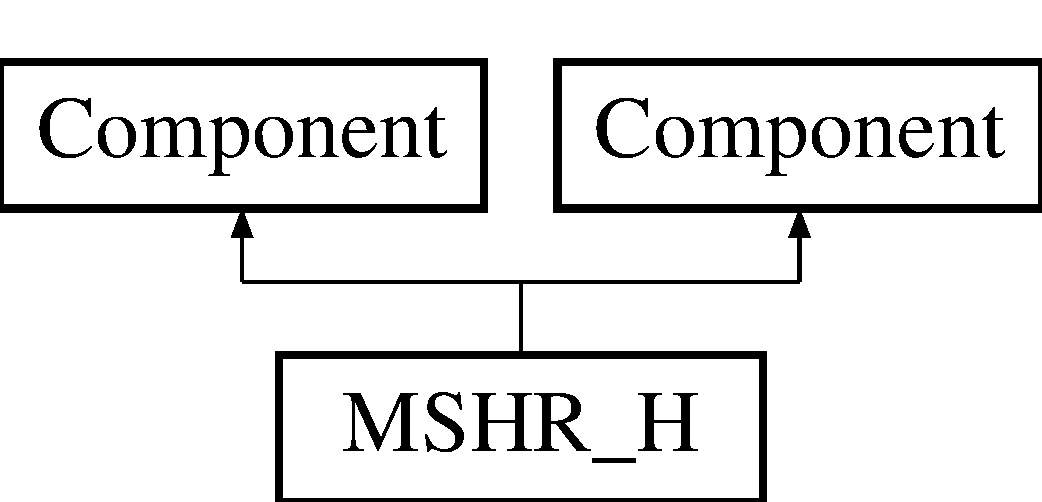
\includegraphics[height=2cm]{classMSHR__H}
\end{center}
\end{figure}
\subsection*{Public Member Functions}
\begin{CompactItemize}
\item 
\hyperlink{classMSHR__H_ed75aac9537ffb4d5814b337c1099e82}{MSHR\_\-H} ()
\item 
\hyperlink{classMSHR__H_cbe3ee20d72b496c43ef9f6375f4da1b}{$\sim$MSHR\_\-H} ()
\item 
\hyperlink{constants_8h_51badf0ffa6471a1e529c69852e56f57}{Addr\_\-t} \hyperlink{classMSHR__H_3c9cdbe3938dcfd521f48678b335b839}{GlobalAddrMap} (\hyperlink{constants_8h_51badf0ffa6471a1e529c69852e56f57}{Addr\_\-t} addr, \hyperlink{constants_8h_ba0996d26f7be2572973245b51852757}{UInt} threadId)
\item 
void \hyperlink{classMSHR__H_1dff946e7d92eae286b8f72df7dc0f03}{process\_\-event} (\hyperlink{classIrisEvent}{IrisEvent} $\ast$e)
\item 
std::string \hyperlink{classMSHR__H_778e0a25bf58c2ccbe506a4c635f953f}{toString} ()
\item 
\hyperlink{classMSHR__H_ed75aac9537ffb4d5814b337c1099e82}{MSHR\_\-H} ()
\item 
\hyperlink{classMSHR__H_cbe3ee20d72b496c43ef9f6375f4da1b}{$\sim$MSHR\_\-H} ()
\item 
\hyperlink{constants_8h_51badf0ffa6471a1e529c69852e56f57}{Addr\_\-t} \hyperlink{classMSHR__H_3c9cdbe3938dcfd521f48678b335b839}{GlobalAddrMap} (\hyperlink{constants_8h_51badf0ffa6471a1e529c69852e56f57}{Addr\_\-t} addr, \hyperlink{constants_8h_ba0996d26f7be2572973245b51852757}{UInt} threadId)
\item 
void \hyperlink{classMSHR__H_1dff946e7d92eae286b8f72df7dc0f03}{process\_\-event} (\hyperlink{classIrisEvent}{IrisEvent} $\ast$e)
\item 
std::string \hyperlink{classMSHR__H_778e0a25bf58c2ccbe506a4c635f953f}{toString} ()
\end{CompactItemize}
\subsection*{Public Attributes}
\begin{CompactItemize}
\item 
\hyperlink{constants_8h_a475e5c84e5eb0fe317942dc62553f7e}{Time} \hyperlink{classMSHR__H_9e26b7281b5d4ec954954209aae9ebfa}{unsink}
\item 
\hyperlink{constants_8h_a475e5c84e5eb0fe317942dc62553f7e}{Time} \hyperlink{classMSHR__H_adfd06c0a14ec47c72e3b3e0c436d62e}{lastFinishTime}
\item 
\hyperlink{constants_8h_a475e5c84e5eb0fe317942dc62553f7e}{Time} \hyperlink{classMSHR__H_08f7e602a70bcf8d0e991d46e19265a2}{globalUnSink}
\item 
bool \hyperlink{classMSHR__H_4cd1713ebd3ab9038ed231781b4bc36a}{done}
\item 
vector$<$ \hyperlink{classRequest}{Request} $>$ \hyperlink{classMSHR__H_a46028543e0902980f6732c2ec1460e1}{mshr}
\item 
vector$<$ \hyperlink{classRequest}{Request} $>$ \hyperlink{classMSHR__H_4b93a7397177a907d0ee3a3cebcbbbda}{writeQueue}
\item 
ifstream \hyperlink{classMSHR__H_6e19d2203f1ad9bf624596e00d600516}{trace\_\-filename}
\item 
char $\ast$ \hyperlink{classMSHR__H_1121ad69747b53dbe515b58094ac7f08}{filename}
\item 
unsigned int \hyperlink{classMSHR__H_97b745c7aeca64268c19411dd6ba5354}{id}
\item 
unsigned int \hyperlink{classMSHR__H_fd269df00bf476b2b151516b64cf7388}{lastScheduledIndex}
\item 
\hyperlink{classComponent}{Component} $\ast$ \hyperlink{classMSHR__H_db1067e0a44f5878fe6c1b7c437f9d93}{parent}
\item 
\hyperlink{classComponent}{Component} $\ast$ \hyperlink{classMSHR__H_66d8569d9e2ea71eb62ef9478761db02}{child}
\end{CompactItemize}


\subsection{Constructor \& Destructor Documentation}
\hypertarget{classMSHR__H_ed75aac9537ffb4d5814b337c1099e82}{
\index{MSHR\_\-H@{MSHR\_\-H}!MSHR\_\-H@{MSHR\_\-H}}
\index{MSHR\_\-H@{MSHR\_\-H}!MSHR_H@{MSHR\_\-H}}
\subsubsection[{MSHR\_\-H}]{\setlength{\rightskip}{0pt plus 5cm}MSHR\_\-H::MSHR\_\-H ()}}
\label{classMSHR__H_ed75aac9537ffb4d5814b337c1099e82}


\hypertarget{classMSHR__H_cbe3ee20d72b496c43ef9f6375f4da1b}{
\index{MSHR\_\-H@{MSHR\_\-H}!$\sim$MSHR\_\-H@{$\sim$MSHR\_\-H}}
\index{$\sim$MSHR\_\-H@{$\sim$MSHR\_\-H}!MSHR_H@{MSHR\_\-H}}
\subsubsection[{$\sim$MSHR\_\-H}]{\setlength{\rightskip}{0pt plus 5cm}MSHR\_\-H::$\sim$MSHR\_\-H ()}}
\label{classMSHR__H_cbe3ee20d72b496c43ef9f6375f4da1b}


\hypertarget{classMSHR__H_ed75aac9537ffb4d5814b337c1099e82}{
\index{MSHR\_\-H@{MSHR\_\-H}!MSHR\_\-H@{MSHR\_\-H}}
\index{MSHR\_\-H@{MSHR\_\-H}!MSHR_H@{MSHR\_\-H}}
\subsubsection[{MSHR\_\-H}]{\setlength{\rightskip}{0pt plus 5cm}MSHR\_\-H::MSHR\_\-H ()}}
\label{classMSHR__H_ed75aac9537ffb4d5814b337c1099e82}


\hypertarget{classMSHR__H_cbe3ee20d72b496c43ef9f6375f4da1b}{
\index{MSHR\_\-H@{MSHR\_\-H}!$\sim$MSHR\_\-H@{$\sim$MSHR\_\-H}}
\index{$\sim$MSHR\_\-H@{$\sim$MSHR\_\-H}!MSHR_H@{MSHR\_\-H}}
\subsubsection[{$\sim$MSHR\_\-H}]{\setlength{\rightskip}{0pt plus 5cm}MSHR\_\-H::$\sim$MSHR\_\-H ()}}
\label{classMSHR__H_cbe3ee20d72b496c43ef9f6375f4da1b}




\subsection{Member Function Documentation}
\hypertarget{classMSHR__H_3c9cdbe3938dcfd521f48678b335b839}{
\index{MSHR\_\-H@{MSHR\_\-H}!GlobalAddrMap@{GlobalAddrMap}}
\index{GlobalAddrMap@{GlobalAddrMap}!MSHR_H@{MSHR\_\-H}}
\subsubsection[{GlobalAddrMap}]{\setlength{\rightskip}{0pt plus 5cm}{\bf Addr\_\-t} MSHR\_\-H::GlobalAddrMap ({\bf Addr\_\-t} {\em addr}, \/  {\bf UInt} {\em threadId})}}
\label{classMSHR__H_3c9cdbe3938dcfd521f48678b335b839}


\hypertarget{classMSHR__H_3c9cdbe3938dcfd521f48678b335b839}{
\index{MSHR\_\-H@{MSHR\_\-H}!GlobalAddrMap@{GlobalAddrMap}}
\index{GlobalAddrMap@{GlobalAddrMap}!MSHR_H@{MSHR\_\-H}}
\subsubsection[{GlobalAddrMap}]{\setlength{\rightskip}{0pt plus 5cm}{\bf Addr\_\-t} MSHR\_\-H::GlobalAddrMap ({\bf Addr\_\-t} {\em addr}, \/  {\bf UInt} {\em threadId})}}
\label{classMSHR__H_3c9cdbe3938dcfd521f48678b335b839}


\hypertarget{classMSHR__H_1dff946e7d92eae286b8f72df7dc0f03}{
\index{MSHR\_\-H@{MSHR\_\-H}!process\_\-event@{process\_\-event}}
\index{process\_\-event@{process\_\-event}!MSHR_H@{MSHR\_\-H}}
\subsubsection[{process\_\-event}]{\setlength{\rightskip}{0pt plus 5cm}void MSHR\_\-H::process\_\-event ({\bf IrisEvent} $\ast$ {\em e})}}
\label{classMSHR__H_1dff946e7d92eae286b8f72df7dc0f03}


\hypertarget{classMSHR__H_1dff946e7d92eae286b8f72df7dc0f03}{
\index{MSHR\_\-H@{MSHR\_\-H}!process\_\-event@{process\_\-event}}
\index{process\_\-event@{process\_\-event}!MSHR_H@{MSHR\_\-H}}
\subsubsection[{process\_\-event}]{\setlength{\rightskip}{0pt plus 5cm}void MSHR\_\-H::process\_\-event ({\bf IrisEvent} $\ast$ {\em e})}}
\label{classMSHR__H_1dff946e7d92eae286b8f72df7dc0f03}


\hypertarget{classMSHR__H_778e0a25bf58c2ccbe506a4c635f953f}{
\index{MSHR\_\-H@{MSHR\_\-H}!toString@{toString}}
\index{toString@{toString}!MSHR_H@{MSHR\_\-H}}
\subsubsection[{toString}]{\setlength{\rightskip}{0pt plus 5cm}std::string MSHR\_\-H::toString ()}}
\label{classMSHR__H_778e0a25bf58c2ccbe506a4c635f953f}


\hypertarget{classMSHR__H_778e0a25bf58c2ccbe506a4c635f953f}{
\index{MSHR\_\-H@{MSHR\_\-H}!toString@{toString}}
\index{toString@{toString}!MSHR_H@{MSHR\_\-H}}
\subsubsection[{toString}]{\setlength{\rightskip}{0pt plus 5cm}std::string MSHR\_\-H::toString ()}}
\label{classMSHR__H_778e0a25bf58c2ccbe506a4c635f953f}




\subsection{Member Data Documentation}
\hypertarget{classMSHR__H_66d8569d9e2ea71eb62ef9478761db02}{
\index{MSHR\_\-H@{MSHR\_\-H}!child@{child}}
\index{child@{child}!MSHR_H@{MSHR\_\-H}}
\subsubsection[{child}]{\setlength{\rightskip}{0pt plus 5cm}{\bf Component} $\ast$ {\bf MSHR\_\-H::child}}}
\label{classMSHR__H_66d8569d9e2ea71eb62ef9478761db02}


\hypertarget{classMSHR__H_4cd1713ebd3ab9038ed231781b4bc36a}{
\index{MSHR\_\-H@{MSHR\_\-H}!done@{done}}
\index{done@{done}!MSHR_H@{MSHR\_\-H}}
\subsubsection[{done}]{\setlength{\rightskip}{0pt plus 5cm}bool {\bf MSHR\_\-H::done}}}
\label{classMSHR__H_4cd1713ebd3ab9038ed231781b4bc36a}


\hypertarget{classMSHR__H_1121ad69747b53dbe515b58094ac7f08}{
\index{MSHR\_\-H@{MSHR\_\-H}!filename@{filename}}
\index{filename@{filename}!MSHR_H@{MSHR\_\-H}}
\subsubsection[{filename}]{\setlength{\rightskip}{0pt plus 5cm}char $\ast$ {\bf MSHR\_\-H::filename}}}
\label{classMSHR__H_1121ad69747b53dbe515b58094ac7f08}


\hypertarget{classMSHR__H_08f7e602a70bcf8d0e991d46e19265a2}{
\index{MSHR\_\-H@{MSHR\_\-H}!globalUnSink@{globalUnSink}}
\index{globalUnSink@{globalUnSink}!MSHR_H@{MSHR\_\-H}}
\subsubsection[{globalUnSink}]{\setlength{\rightskip}{0pt plus 5cm}{\bf Time} {\bf MSHR\_\-H::globalUnSink}}}
\label{classMSHR__H_08f7e602a70bcf8d0e991d46e19265a2}


\hypertarget{classMSHR__H_97b745c7aeca64268c19411dd6ba5354}{
\index{MSHR\_\-H@{MSHR\_\-H}!id@{id}}
\index{id@{id}!MSHR_H@{MSHR\_\-H}}
\subsubsection[{id}]{\setlength{\rightskip}{0pt plus 5cm}unsigned int {\bf MSHR\_\-H::id}}}
\label{classMSHR__H_97b745c7aeca64268c19411dd6ba5354}


\hypertarget{classMSHR__H_adfd06c0a14ec47c72e3b3e0c436d62e}{
\index{MSHR\_\-H@{MSHR\_\-H}!lastFinishTime@{lastFinishTime}}
\index{lastFinishTime@{lastFinishTime}!MSHR_H@{MSHR\_\-H}}
\subsubsection[{lastFinishTime}]{\setlength{\rightskip}{0pt plus 5cm}{\bf Time} {\bf MSHR\_\-H::lastFinishTime}}}
\label{classMSHR__H_adfd06c0a14ec47c72e3b3e0c436d62e}


\hypertarget{classMSHR__H_fd269df00bf476b2b151516b64cf7388}{
\index{MSHR\_\-H@{MSHR\_\-H}!lastScheduledIndex@{lastScheduledIndex}}
\index{lastScheduledIndex@{lastScheduledIndex}!MSHR_H@{MSHR\_\-H}}
\subsubsection[{lastScheduledIndex}]{\setlength{\rightskip}{0pt plus 5cm}unsigned int {\bf MSHR\_\-H::lastScheduledIndex}}}
\label{classMSHR__H_fd269df00bf476b2b151516b64cf7388}


\hypertarget{classMSHR__H_a46028543e0902980f6732c2ec1460e1}{
\index{MSHR\_\-H@{MSHR\_\-H}!mshr@{mshr}}
\index{mshr@{mshr}!MSHR_H@{MSHR\_\-H}}
\subsubsection[{mshr}]{\setlength{\rightskip}{0pt plus 5cm}vector$<$ {\bf Request} $>$ {\bf MSHR\_\-H::mshr}}}
\label{classMSHR__H_a46028543e0902980f6732c2ec1460e1}


\hypertarget{classMSHR__H_db1067e0a44f5878fe6c1b7c437f9d93}{
\index{MSHR\_\-H@{MSHR\_\-H}!parent@{parent}}
\index{parent@{parent}!MSHR_H@{MSHR\_\-H}}
\subsubsection[{parent}]{\setlength{\rightskip}{0pt plus 5cm}{\bf Component} $\ast$ {\bf MSHR\_\-H::parent}}}
\label{classMSHR__H_db1067e0a44f5878fe6c1b7c437f9d93}


\hypertarget{classMSHR__H_6e19d2203f1ad9bf624596e00d600516}{
\index{MSHR\_\-H@{MSHR\_\-H}!trace\_\-filename@{trace\_\-filename}}
\index{trace\_\-filename@{trace\_\-filename}!MSHR_H@{MSHR\_\-H}}
\subsubsection[{trace\_\-filename}]{\setlength{\rightskip}{0pt plus 5cm}ifstream {\bf MSHR\_\-H::trace\_\-filename}}}
\label{classMSHR__H_6e19d2203f1ad9bf624596e00d600516}


\hypertarget{classMSHR__H_9e26b7281b5d4ec954954209aae9ebfa}{
\index{MSHR\_\-H@{MSHR\_\-H}!unsink@{unsink}}
\index{unsink@{unsink}!MSHR_H@{MSHR\_\-H}}
\subsubsection[{unsink}]{\setlength{\rightskip}{0pt plus 5cm}{\bf Time} {\bf MSHR\_\-H::unsink}}}
\label{classMSHR__H_9e26b7281b5d4ec954954209aae9ebfa}


\hypertarget{classMSHR__H_4b93a7397177a907d0ee3a3cebcbbbda}{
\index{MSHR\_\-H@{MSHR\_\-H}!writeQueue@{writeQueue}}
\index{writeQueue@{writeQueue}!MSHR_H@{MSHR\_\-H}}
\subsubsection[{writeQueue}]{\setlength{\rightskip}{0pt plus 5cm}vector$<$ {\bf Request} $>$ {\bf MSHR\_\-H::writeQueue}}}
\label{classMSHR__H_4b93a7397177a907d0ee3a3cebcbbbda}




The documentation for this class was generated from the following files:\begin{CompactItemize}
\item 
source/components/impl/\hyperlink{impl_2mshr_8h}{mshr.h}\item 
source/components/none/\hyperlink{none_2mshr_8h}{mshr.h}\item 
source/components/impl/\hyperlink{impl_2mshr_8cc}{mshr.cc}\item 
source/components/none/\hyperlink{none_2mshr_8cc}{mshr.cc}\end{CompactItemize}

\hypertarget{classMTRand}{
\section{MTRand Class Reference}
\label{classMTRand}\index{MTRand@{MTRand}}
}
{\tt \#include $<$MersenneTwister.h$>$}

\subsection*{Public Types}
\begin{CompactItemize}
\item 
enum \{ \hyperlink{classMTRand_b8fea37d16b55e1a0fe06149e325f1b660f472facea8fabd42765cd91273db7b}{N} =  624
 \}
\item 
enum \{ \hyperlink{classMTRand_7d9f4f1783a4e45f7834dd5174dfc2a13899803ea0d4da3018d311ed4902d9cc}{SAVE} =  N + 1
 \}
\item 
typedef unsigned long \hyperlink{classMTRand_45478edf9e24dcd2a5164bac3889d6a2}{uint32}
\subsection*{Public Member Functions}
\begin{CompactItemize}
\item 
\hyperlink{classMTRand_172bc7e7cf1e578ef3f9c90a8cee3eb1}{MTRand} (const \hyperlink{classMTRand_45478edf9e24dcd2a5164bac3889d6a2}{uint32} oneSeed)
\item 
\hyperlink{classMTRand_380e79e0192b46426abcefa6e2dd082e}{MTRand} (\hyperlink{classMTRand_45478edf9e24dcd2a5164bac3889d6a2}{uint32} $\ast$const bigSeed, \hyperlink{classMTRand_45478edf9e24dcd2a5164bac3889d6a2}{uint32} const seedLength=N)
\item 
\hyperlink{classMTRand_265dc65546e26073c0d5f8787b045a1d}{MTRand} ()
\item 
\hyperlink{classMTRand_ff69d4a4ec88475bab03a295e8fb0f60}{MTRand} (const \hyperlink{classMTRand}{MTRand} \&o)
\item 
\hyperlink{classMTRand_45478edf9e24dcd2a5164bac3889d6a2}{uint32} \hyperlink{classMTRand_d1008efd4fe0e8aae30459c2c58cfe35}{randInt} ()
\item 
\hyperlink{classMTRand_45478edf9e24dcd2a5164bac3889d6a2}{uint32} \hyperlink{classMTRand_3515bbf6e1b46680a4ce6968451942b6}{randInt} (const \hyperlink{classMTRand_45478edf9e24dcd2a5164bac3889d6a2}{uint32} n)
\item 
double \hyperlink{classMTRand_76d129a2d850c24ff4a0613f299cf3a5}{rand} ()
\item 
double \hyperlink{classMTRand_a4fe82fc27fd81414ce7554093a9766b}{rand} (const double n)
\item 
double \hyperlink{classMTRand_fd05e468983b3a3d66ce0f403bd666af}{randExc} ()
\item 
double \hyperlink{classMTRand_a1e89d6c7ac8737567b3ccf8fe70b6de}{randExc} (const double n)
\item 
double \hyperlink{classMTRand_4d3a475aa72fe6d1a6d7d9e16d6a732e}{randDblExc} ()
\item 
double \hyperlink{classMTRand_1a81d8f00de8f553d4b8626d64e1c544}{randDblExc} (const double n)
\item 
double \hyperlink{classMTRand_bbb87a08d622d58fdee0eea4cb5471a0}{operator()} ()
\item 
double \hyperlink{classMTRand_15f4daf79febbe4ff43c3e6ce2c4fcbe}{rand53} ()
\item 
double \hyperlink{classMTRand_4c284f626b6d40a0367ff2a949ea1944}{randNorm} (const double mean=0.0, const double stddev=1.0)
\item 
void \hyperlink{classMTRand_1e21a79e0a30225fffe924229e34a923}{seed} (const \hyperlink{classMTRand_45478edf9e24dcd2a5164bac3889d6a2}{uint32} oneSeed)
\item 
void \hyperlink{classMTRand_5758103776b131e8ea46b6dc1b9fb267}{seed} (\hyperlink{classMTRand_45478edf9e24dcd2a5164bac3889d6a2}{uint32} $\ast$const bigSeed, const \hyperlink{classMTRand_45478edf9e24dcd2a5164bac3889d6a2}{uint32} seedLength=N)
\item 
void \hyperlink{classMTRand_d88ea3363d55bafb62826bbd130279c2}{seed} ()
\item 
void \hyperlink{classMTRand_d60e0f3f5c90baab75b74f9a2ccae871}{save} (\hyperlink{classMTRand_45478edf9e24dcd2a5164bac3889d6a2}{uint32} $\ast$saveArray) const 
\item 
void \hyperlink{classMTRand_8302e9a8cd16d8dfc536a85bf2f68be0}{load} (\hyperlink{classMTRand_45478edf9e24dcd2a5164bac3889d6a2}{uint32} $\ast$const loadArray)
\item 
\hyperlink{classMTRand}{MTRand} \& \hyperlink{classMTRand_3a6eb21add6f6ef4ce2d3280f2518521}{operator=} (const \hyperlink{classMTRand}{MTRand} \&o)
\end{CompactItemize}
\subsection*{Protected Types}
\begin{CompactItemize}
\item 
enum \{ \hyperlink{classMTRand_10c3437be98225f5b0beee1ed8c033c8133070000b798889cd75535ea0d5bb71}{M} =  397
 \}
\subsection*{Protected Member Functions}
\begin{CompactItemize}
\item 
void \hyperlink{classMTRand_9b9a20998f5c805af6301ce5c37dcfc3}{initialize} (const \hyperlink{classMTRand_45478edf9e24dcd2a5164bac3889d6a2}{uint32} oneSeed)
\item 
void \hyperlink{classMTRand_1d5fcb69d83f4d2fd653883c8352f86c}{reload} ()
\item 
\hyperlink{classMTRand_45478edf9e24dcd2a5164bac3889d6a2}{uint32} \hyperlink{classMTRand_45eea926a0602e4bb5c0b90b04779826}{hiBit} (const \hyperlink{classMTRand_45478edf9e24dcd2a5164bac3889d6a2}{uint32} u) const 
\item 
\hyperlink{classMTRand_45478edf9e24dcd2a5164bac3889d6a2}{uint32} \hyperlink{classMTRand_6f5a4a532e1c3acd42052046594205be}{loBit} (const \hyperlink{classMTRand_45478edf9e24dcd2a5164bac3889d6a2}{uint32} u) const 
\item 
\hyperlink{classMTRand_45478edf9e24dcd2a5164bac3889d6a2}{uint32} \hyperlink{classMTRand_d846f81f7abfc1b20c51d1563b8e5d45}{loBits} (const \hyperlink{classMTRand_45478edf9e24dcd2a5164bac3889d6a2}{uint32} u) const 
\item 
\hyperlink{classMTRand_45478edf9e24dcd2a5164bac3889d6a2}{uint32} \hyperlink{classMTRand_bdd5587252ed1ac89cb274e4bf4881da}{mixBits} (const \hyperlink{classMTRand_45478edf9e24dcd2a5164bac3889d6a2}{uint32} u, const \hyperlink{classMTRand_45478edf9e24dcd2a5164bac3889d6a2}{uint32} v) const 
\item 
\hyperlink{classMTRand_45478edf9e24dcd2a5164bac3889d6a2}{uint32} \hyperlink{classMTRand_8539a48116c85704c5101981cb0823e7}{magic} (const \hyperlink{classMTRand_45478edf9e24dcd2a5164bac3889d6a2}{uint32} u) const 
\item 
\hyperlink{classMTRand_45478edf9e24dcd2a5164bac3889d6a2}{uint32} \hyperlink{classMTRand_cf32530212717166e3d02dd3cc0b68c4}{twist} (const \hyperlink{classMTRand_45478edf9e24dcd2a5164bac3889d6a2}{uint32} m, const \hyperlink{classMTRand_45478edf9e24dcd2a5164bac3889d6a2}{uint32} s0, const \hyperlink{classMTRand_45478edf9e24dcd2a5164bac3889d6a2}{uint32} s1) const 
\end{CompactItemize}
\subsection*{Static Protected Member Functions}
\begin{CompactItemize}
\item 
static \hyperlink{classMTRand_45478edf9e24dcd2a5164bac3889d6a2}{uint32} \hyperlink{classMTRand_486885d03f38c844315d002e6312fa23}{hash} (time\_\-t t, clock\_\-t c)
\end{CompactItemize}
\subsection*{Protected Attributes}
\begin{CompactItemize}
\item 
\hyperlink{classMTRand_45478edf9e24dcd2a5164bac3889d6a2}{uint32} \hyperlink{classMTRand_2c87f537429bf0b0f6a452c22b9eebba}{state} \mbox{[}N\mbox{]}
\item 
\hyperlink{classMTRand_45478edf9e24dcd2a5164bac3889d6a2}{uint32} $\ast$ \hyperlink{classMTRand_2b80858137c88fe69d4d2bdc665bcf93}{pNext}
\item 
int \hyperlink{classMTRand_98eabf568c88f121e44f487397f32495}{left}
\end{CompactItemize}
\subsection*{Friends}
\begin{CompactItemize}
\item 
std::ostream \& \hyperlink{classMTRand_059061d50a1e54ee3067d4e1dbdd7c64}{operator$<$$<$} (std::ostream \&os, const \hyperlink{classMTRand}{MTRand} \&mtrand)
\item 
std::istream \& \hyperlink{classMTRand_45b02a702835a3be42171c5c2dc79b2d}{operator$>$$>$} (std::istream \&is, \hyperlink{classMTRand}{MTRand} \&mtrand)
\end{CompactItemize}


\subsection{Member Typedef Documentation}
\hypertarget{classMTRand_45478edf9e24dcd2a5164bac3889d6a2}{
\index{MTRand@{MTRand}!uint32@{uint32}}
\index{uint32@{uint32}!MTRand@{MTRand}}
\subsubsection[{uint32}]{\setlength{\rightskip}{0pt plus 5cm}typedef unsigned long {\bf MTRand::uint32}}}
\label{classMTRand_45478edf9e24dcd2a5164bac3889d6a2}




\subsection{Member Enumeration Documentation}
\hypertarget{classMTRand_b8fea37d16b55e1a0fe06149e325f1b6}{
\subsubsection[{"@0}]{\setlength{\rightskip}{0pt plus 5cm}anonymous enum}}
\label{classMTRand_b8fea37d16b55e1a0fe06149e325f1b6}


\begin{Desc}
\item[Enumerator: ]\par
\begin{description}
\index{N@{N}!MTRand@{MTRand}}\index{MTRand@{MTRand}!N@{N}}\item[{\em 
\hypertarget{classMTRand_b8fea37d16b55e1a0fe06149e325f1b660f472facea8fabd42765cd91273db7b}{
N}
\label{classMTRand_b8fea37d16b55e1a0fe06149e325f1b660f472facea8fabd42765cd91273db7b}
}]\end{description}
\end{Desc}

\hypertarget{classMTRand_7d9f4f1783a4e45f7834dd5174dfc2a1}{
\subsubsection[{"@1}]{\setlength{\rightskip}{0pt plus 5cm}anonymous enum}}
\label{classMTRand_7d9f4f1783a4e45f7834dd5174dfc2a1}


\begin{Desc}
\item[Enumerator: ]\par
\begin{description}
\index{SAVE@{SAVE}!MTRand@{MTRand}}\index{MTRand@{MTRand}!SAVE@{SAVE}}\item[{\em 
\hypertarget{classMTRand_7d9f4f1783a4e45f7834dd5174dfc2a13899803ea0d4da3018d311ed4902d9cc}{
SAVE}
\label{classMTRand_7d9f4f1783a4e45f7834dd5174dfc2a13899803ea0d4da3018d311ed4902d9cc}
}]\end{description}
\end{Desc}

\hypertarget{classMTRand_10c3437be98225f5b0beee1ed8c033c8}{
\subsubsection[{"@2}]{\setlength{\rightskip}{0pt plus 5cm}anonymous enum\hspace{0.3cm}{\tt  \mbox{[}protected\mbox{]}}}}
\label{classMTRand_10c3437be98225f5b0beee1ed8c033c8}


\begin{Desc}
\item[Enumerator: ]\par
\begin{description}
\index{M@{M}!MTRand@{MTRand}}\index{MTRand@{MTRand}!M@{M}}\item[{\em 
\hypertarget{classMTRand_10c3437be98225f5b0beee1ed8c033c8133070000b798889cd75535ea0d5bb71}{
M}
\label{classMTRand_10c3437be98225f5b0beee1ed8c033c8133070000b798889cd75535ea0d5bb71}
}]\end{description}
\end{Desc}



\subsection{Constructor \& Destructor Documentation}
\hypertarget{classMTRand_172bc7e7cf1e578ef3f9c90a8cee3eb1}{
\index{MTRand@{MTRand}!MTRand@{MTRand}}
\index{MTRand@{MTRand}!MTRand@{MTRand}}
\subsubsection[{MTRand}]{\setlength{\rightskip}{0pt plus 5cm}MTRand::MTRand (const {\bf uint32} {\em oneSeed})\hspace{0.3cm}{\tt  \mbox{[}inline\mbox{]}}}}
\label{classMTRand_172bc7e7cf1e578ef3f9c90a8cee3eb1}


\hypertarget{classMTRand_380e79e0192b46426abcefa6e2dd082e}{
\index{MTRand@{MTRand}!MTRand@{MTRand}}
\index{MTRand@{MTRand}!MTRand@{MTRand}}
\subsubsection[{MTRand}]{\setlength{\rightskip}{0pt plus 5cm}MTRand::MTRand ({\bf uint32} $\ast$const  {\em bigSeed}, \/  {\bf uint32} const {\em seedLength} = {\tt N})\hspace{0.3cm}{\tt  \mbox{[}inline\mbox{]}}}}
\label{classMTRand_380e79e0192b46426abcefa6e2dd082e}


\hypertarget{classMTRand_265dc65546e26073c0d5f8787b045a1d}{
\index{MTRand@{MTRand}!MTRand@{MTRand}}
\index{MTRand@{MTRand}!MTRand@{MTRand}}
\subsubsection[{MTRand}]{\setlength{\rightskip}{0pt plus 5cm}MTRand::MTRand ()\hspace{0.3cm}{\tt  \mbox{[}inline\mbox{]}}}}
\label{classMTRand_265dc65546e26073c0d5f8787b045a1d}


\hypertarget{classMTRand_ff69d4a4ec88475bab03a295e8fb0f60}{
\index{MTRand@{MTRand}!MTRand@{MTRand}}
\index{MTRand@{MTRand}!MTRand@{MTRand}}
\subsubsection[{MTRand}]{\setlength{\rightskip}{0pt plus 5cm}MTRand::MTRand (const {\bf MTRand} \& {\em o})\hspace{0.3cm}{\tt  \mbox{[}inline\mbox{]}}}}
\label{classMTRand_ff69d4a4ec88475bab03a295e8fb0f60}




\subsection{Member Function Documentation}
\hypertarget{classMTRand_486885d03f38c844315d002e6312fa23}{
\index{MTRand@{MTRand}!hash@{hash}}
\index{hash@{hash}!MTRand@{MTRand}}
\subsubsection[{hash}]{\setlength{\rightskip}{0pt plus 5cm}{\bf MTRand::uint32} MTRand::hash (time\_\-t {\em t}, \/  clock\_\-t {\em c})\hspace{0.3cm}{\tt  \mbox{[}inline, static, protected\mbox{]}}}}
\label{classMTRand_486885d03f38c844315d002e6312fa23}


\hypertarget{classMTRand_45eea926a0602e4bb5c0b90b04779826}{
\index{MTRand@{MTRand}!hiBit@{hiBit}}
\index{hiBit@{hiBit}!MTRand@{MTRand}}
\subsubsection[{hiBit}]{\setlength{\rightskip}{0pt plus 5cm}{\bf uint32} MTRand::hiBit (const {\bf uint32} {\em u}) const\hspace{0.3cm}{\tt  \mbox{[}inline, protected\mbox{]}}}}
\label{classMTRand_45eea926a0602e4bb5c0b90b04779826}


\hypertarget{classMTRand_9b9a20998f5c805af6301ce5c37dcfc3}{
\index{MTRand@{MTRand}!initialize@{initialize}}
\index{initialize@{initialize}!MTRand@{MTRand}}
\subsubsection[{initialize}]{\setlength{\rightskip}{0pt plus 5cm}void MTRand::initialize (const {\bf uint32} {\em oneSeed})\hspace{0.3cm}{\tt  \mbox{[}inline, protected\mbox{]}}}}
\label{classMTRand_9b9a20998f5c805af6301ce5c37dcfc3}


\hypertarget{classMTRand_8302e9a8cd16d8dfc536a85bf2f68be0}{
\index{MTRand@{MTRand}!load@{load}}
\index{load@{load}!MTRand@{MTRand}}
\subsubsection[{load}]{\setlength{\rightskip}{0pt plus 5cm}void MTRand::load ({\bf uint32} $\ast$const  {\em loadArray})\hspace{0.3cm}{\tt  \mbox{[}inline\mbox{]}}}}
\label{classMTRand_8302e9a8cd16d8dfc536a85bf2f68be0}


\hypertarget{classMTRand_6f5a4a532e1c3acd42052046594205be}{
\index{MTRand@{MTRand}!loBit@{loBit}}
\index{loBit@{loBit}!MTRand@{MTRand}}
\subsubsection[{loBit}]{\setlength{\rightskip}{0pt plus 5cm}{\bf uint32} MTRand::loBit (const {\bf uint32} {\em u}) const\hspace{0.3cm}{\tt  \mbox{[}inline, protected\mbox{]}}}}
\label{classMTRand_6f5a4a532e1c3acd42052046594205be}


\hypertarget{classMTRand_d846f81f7abfc1b20c51d1563b8e5d45}{
\index{MTRand@{MTRand}!loBits@{loBits}}
\index{loBits@{loBits}!MTRand@{MTRand}}
\subsubsection[{loBits}]{\setlength{\rightskip}{0pt plus 5cm}{\bf uint32} MTRand::loBits (const {\bf uint32} {\em u}) const\hspace{0.3cm}{\tt  \mbox{[}inline, protected\mbox{]}}}}
\label{classMTRand_d846f81f7abfc1b20c51d1563b8e5d45}


\hypertarget{classMTRand_8539a48116c85704c5101981cb0823e7}{
\index{MTRand@{MTRand}!magic@{magic}}
\index{magic@{magic}!MTRand@{MTRand}}
\subsubsection[{magic}]{\setlength{\rightskip}{0pt plus 5cm}{\bf uint32} MTRand::magic (const {\bf uint32} {\em u}) const\hspace{0.3cm}{\tt  \mbox{[}inline, protected\mbox{]}}}}
\label{classMTRand_8539a48116c85704c5101981cb0823e7}


\hypertarget{classMTRand_bdd5587252ed1ac89cb274e4bf4881da}{
\index{MTRand@{MTRand}!mixBits@{mixBits}}
\index{mixBits@{mixBits}!MTRand@{MTRand}}
\subsubsection[{mixBits}]{\setlength{\rightskip}{0pt plus 5cm}{\bf uint32} MTRand::mixBits (const {\bf uint32} {\em u}, \/  const {\bf uint32} {\em v}) const\hspace{0.3cm}{\tt  \mbox{[}inline, protected\mbox{]}}}}
\label{classMTRand_bdd5587252ed1ac89cb274e4bf4881da}


\hypertarget{classMTRand_bbb87a08d622d58fdee0eea4cb5471a0}{
\index{MTRand@{MTRand}!operator()@{operator()}}
\index{operator()@{operator()}!MTRand@{MTRand}}
\subsubsection[{operator()}]{\setlength{\rightskip}{0pt plus 5cm}double MTRand::operator() ()\hspace{0.3cm}{\tt  \mbox{[}inline\mbox{]}}}}
\label{classMTRand_bbb87a08d622d58fdee0eea4cb5471a0}


\hypertarget{classMTRand_3a6eb21add6f6ef4ce2d3280f2518521}{
\index{MTRand@{MTRand}!operator=@{operator=}}
\index{operator=@{operator=}!MTRand@{MTRand}}
\subsubsection[{operator=}]{\setlength{\rightskip}{0pt plus 5cm}{\bf MTRand} \& MTRand::operator= (const {\bf MTRand} \& {\em o})\hspace{0.3cm}{\tt  \mbox{[}inline\mbox{]}}}}
\label{classMTRand_3a6eb21add6f6ef4ce2d3280f2518521}


\hypertarget{classMTRand_a4fe82fc27fd81414ce7554093a9766b}{
\index{MTRand@{MTRand}!rand@{rand}}
\index{rand@{rand}!MTRand@{MTRand}}
\subsubsection[{rand}]{\setlength{\rightskip}{0pt plus 5cm}double MTRand::rand (const double {\em n})\hspace{0.3cm}{\tt  \mbox{[}inline\mbox{]}}}}
\label{classMTRand_a4fe82fc27fd81414ce7554093a9766b}


\hypertarget{classMTRand_76d129a2d850c24ff4a0613f299cf3a5}{
\index{MTRand@{MTRand}!rand@{rand}}
\index{rand@{rand}!MTRand@{MTRand}}
\subsubsection[{rand}]{\setlength{\rightskip}{0pt plus 5cm}double MTRand::rand ()\hspace{0.3cm}{\tt  \mbox{[}inline\mbox{]}}}}
\label{classMTRand_76d129a2d850c24ff4a0613f299cf3a5}


\hypertarget{classMTRand_15f4daf79febbe4ff43c3e6ce2c4fcbe}{
\index{MTRand@{MTRand}!rand53@{rand53}}
\index{rand53@{rand53}!MTRand@{MTRand}}
\subsubsection[{rand53}]{\setlength{\rightskip}{0pt plus 5cm}double MTRand::rand53 ()\hspace{0.3cm}{\tt  \mbox{[}inline\mbox{]}}}}
\label{classMTRand_15f4daf79febbe4ff43c3e6ce2c4fcbe}


\hypertarget{classMTRand_1a81d8f00de8f553d4b8626d64e1c544}{
\index{MTRand@{MTRand}!randDblExc@{randDblExc}}
\index{randDblExc@{randDblExc}!MTRand@{MTRand}}
\subsubsection[{randDblExc}]{\setlength{\rightskip}{0pt plus 5cm}double MTRand::randDblExc (const double {\em n})\hspace{0.3cm}{\tt  \mbox{[}inline\mbox{]}}}}
\label{classMTRand_1a81d8f00de8f553d4b8626d64e1c544}


\hypertarget{classMTRand_4d3a475aa72fe6d1a6d7d9e16d6a732e}{
\index{MTRand@{MTRand}!randDblExc@{randDblExc}}
\index{randDblExc@{randDblExc}!MTRand@{MTRand}}
\subsubsection[{randDblExc}]{\setlength{\rightskip}{0pt plus 5cm}double MTRand::randDblExc ()\hspace{0.3cm}{\tt  \mbox{[}inline\mbox{]}}}}
\label{classMTRand_4d3a475aa72fe6d1a6d7d9e16d6a732e}


\hypertarget{classMTRand_a1e89d6c7ac8737567b3ccf8fe70b6de}{
\index{MTRand@{MTRand}!randExc@{randExc}}
\index{randExc@{randExc}!MTRand@{MTRand}}
\subsubsection[{randExc}]{\setlength{\rightskip}{0pt plus 5cm}double MTRand::randExc (const double {\em n})\hspace{0.3cm}{\tt  \mbox{[}inline\mbox{]}}}}
\label{classMTRand_a1e89d6c7ac8737567b3ccf8fe70b6de}


\hypertarget{classMTRand_fd05e468983b3a3d66ce0f403bd666af}{
\index{MTRand@{MTRand}!randExc@{randExc}}
\index{randExc@{randExc}!MTRand@{MTRand}}
\subsubsection[{randExc}]{\setlength{\rightskip}{0pt plus 5cm}double MTRand::randExc ()\hspace{0.3cm}{\tt  \mbox{[}inline\mbox{]}}}}
\label{classMTRand_fd05e468983b3a3d66ce0f403bd666af}


\hypertarget{classMTRand_3515bbf6e1b46680a4ce6968451942b6}{
\index{MTRand@{MTRand}!randInt@{randInt}}
\index{randInt@{randInt}!MTRand@{MTRand}}
\subsubsection[{randInt}]{\setlength{\rightskip}{0pt plus 5cm}{\bf MTRand::uint32} MTRand::randInt (const {\bf uint32} {\em n})\hspace{0.3cm}{\tt  \mbox{[}inline\mbox{]}}}}
\label{classMTRand_3515bbf6e1b46680a4ce6968451942b6}


\hypertarget{classMTRand_d1008efd4fe0e8aae30459c2c58cfe35}{
\index{MTRand@{MTRand}!randInt@{randInt}}
\index{randInt@{randInt}!MTRand@{MTRand}}
\subsubsection[{randInt}]{\setlength{\rightskip}{0pt plus 5cm}{\bf MTRand::uint32} MTRand::randInt ()\hspace{0.3cm}{\tt  \mbox{[}inline\mbox{]}}}}
\label{classMTRand_d1008efd4fe0e8aae30459c2c58cfe35}


\hypertarget{classMTRand_4c284f626b6d40a0367ff2a949ea1944}{
\index{MTRand@{MTRand}!randNorm@{randNorm}}
\index{randNorm@{randNorm}!MTRand@{MTRand}}
\subsubsection[{randNorm}]{\setlength{\rightskip}{0pt plus 5cm}double MTRand::randNorm (const double {\em mean} = {\tt 0.0}, \/  const double {\em stddev} = {\tt 1.0})\hspace{0.3cm}{\tt  \mbox{[}inline\mbox{]}}}}
\label{classMTRand_4c284f626b6d40a0367ff2a949ea1944}


\hypertarget{classMTRand_1d5fcb69d83f4d2fd653883c8352f86c}{
\index{MTRand@{MTRand}!reload@{reload}}
\index{reload@{reload}!MTRand@{MTRand}}
\subsubsection[{reload}]{\setlength{\rightskip}{0pt plus 5cm}void MTRand::reload ()\hspace{0.3cm}{\tt  \mbox{[}inline, protected\mbox{]}}}}
\label{classMTRand_1d5fcb69d83f4d2fd653883c8352f86c}


\hypertarget{classMTRand_d60e0f3f5c90baab75b74f9a2ccae871}{
\index{MTRand@{MTRand}!save@{save}}
\index{save@{save}!MTRand@{MTRand}}
\subsubsection[{save}]{\setlength{\rightskip}{0pt plus 5cm}void MTRand::save ({\bf uint32} $\ast$ {\em saveArray}) const\hspace{0.3cm}{\tt  \mbox{[}inline\mbox{]}}}}
\label{classMTRand_d60e0f3f5c90baab75b74f9a2ccae871}


\hypertarget{classMTRand_d88ea3363d55bafb62826bbd130279c2}{
\index{MTRand@{MTRand}!seed@{seed}}
\index{seed@{seed}!MTRand@{MTRand}}
\subsubsection[{seed}]{\setlength{\rightskip}{0pt plus 5cm}void MTRand::seed ()\hspace{0.3cm}{\tt  \mbox{[}inline\mbox{]}}}}
\label{classMTRand_d88ea3363d55bafb62826bbd130279c2}


\hypertarget{classMTRand_5758103776b131e8ea46b6dc1b9fb267}{
\index{MTRand@{MTRand}!seed@{seed}}
\index{seed@{seed}!MTRand@{MTRand}}
\subsubsection[{seed}]{\setlength{\rightskip}{0pt plus 5cm}void MTRand::seed ({\bf uint32} $\ast$const  {\em bigSeed}, \/  const {\bf uint32} {\em seedLength} = {\tt N})\hspace{0.3cm}{\tt  \mbox{[}inline\mbox{]}}}}
\label{classMTRand_5758103776b131e8ea46b6dc1b9fb267}


\hypertarget{classMTRand_1e21a79e0a30225fffe924229e34a923}{
\index{MTRand@{MTRand}!seed@{seed}}
\index{seed@{seed}!MTRand@{MTRand}}
\subsubsection[{seed}]{\setlength{\rightskip}{0pt plus 5cm}void MTRand::seed (const {\bf uint32} {\em oneSeed})\hspace{0.3cm}{\tt  \mbox{[}inline\mbox{]}}}}
\label{classMTRand_1e21a79e0a30225fffe924229e34a923}


\hypertarget{classMTRand_cf32530212717166e3d02dd3cc0b68c4}{
\index{MTRand@{MTRand}!twist@{twist}}
\index{twist@{twist}!MTRand@{MTRand}}
\subsubsection[{twist}]{\setlength{\rightskip}{0pt plus 5cm}{\bf uint32} MTRand::twist (const {\bf uint32} {\em m}, \/  const {\bf uint32} {\em s0}, \/  const {\bf uint32} {\em s1}) const\hspace{0.3cm}{\tt  \mbox{[}inline, protected\mbox{]}}}}
\label{classMTRand_cf32530212717166e3d02dd3cc0b68c4}




\subsection{Friends And Related Function Documentation}
\hypertarget{classMTRand_059061d50a1e54ee3067d4e1dbdd7c64}{
\index{MTRand@{MTRand}!operator$<$$<$@{operator$<$$<$}}
\index{operator$<$$<$@{operator$<$$<$}!MTRand@{MTRand}}
\subsubsection[{operator$<$$<$}]{\setlength{\rightskip}{0pt plus 5cm}std::ostream\& operator$<$$<$ (std::ostream \& {\em os}, \/  const {\bf MTRand} \& {\em mtrand})\hspace{0.3cm}{\tt  \mbox{[}friend\mbox{]}}}}
\label{classMTRand_059061d50a1e54ee3067d4e1dbdd7c64}


\hypertarget{classMTRand_45b02a702835a3be42171c5c2dc79b2d}{
\index{MTRand@{MTRand}!operator$>$$>$@{operator$>$$>$}}
\index{operator$>$$>$@{operator$>$$>$}!MTRand@{MTRand}}
\subsubsection[{operator$>$$>$}]{\setlength{\rightskip}{0pt plus 5cm}std::istream\& operator$>$$>$ (std::istream \& {\em is}, \/  {\bf MTRand} \& {\em mtrand})\hspace{0.3cm}{\tt  \mbox{[}friend\mbox{]}}}}
\label{classMTRand_45b02a702835a3be42171c5c2dc79b2d}




\subsection{Member Data Documentation}
\hypertarget{classMTRand_98eabf568c88f121e44f487397f32495}{
\index{MTRand@{MTRand}!left@{left}}
\index{left@{left}!MTRand@{MTRand}}
\subsubsection[{left}]{\setlength{\rightskip}{0pt plus 5cm}int {\bf MTRand::left}\hspace{0.3cm}{\tt  \mbox{[}protected\mbox{]}}}}
\label{classMTRand_98eabf568c88f121e44f487397f32495}


\hypertarget{classMTRand_2b80858137c88fe69d4d2bdc665bcf93}{
\index{MTRand@{MTRand}!pNext@{pNext}}
\index{pNext@{pNext}!MTRand@{MTRand}}
\subsubsection[{pNext}]{\setlength{\rightskip}{0pt plus 5cm}{\bf uint32}$\ast$ {\bf MTRand::pNext}\hspace{0.3cm}{\tt  \mbox{[}protected\mbox{]}}}}
\label{classMTRand_2b80858137c88fe69d4d2bdc665bcf93}


\hypertarget{classMTRand_2c87f537429bf0b0f6a452c22b9eebba}{
\index{MTRand@{MTRand}!state@{state}}
\index{state@{state}!MTRand@{MTRand}}
\subsubsection[{state}]{\setlength{\rightskip}{0pt plus 5cm}{\bf uint32} {\bf MTRand::state}\mbox{[}N\mbox{]}\hspace{0.3cm}{\tt  \mbox{[}protected\mbox{]}}}}
\label{classMTRand_2c87f537429bf0b0f6a452c22b9eebba}




The documentation for this class was generated from the following file:\begin{CompactItemize}
\item 
source/tests/\hyperlink{MersenneTwister_8h}{MersenneTwister.h}\end{CompactItemize}

\hypertarget{classMyArbiter}{
\section{MyArbiter Class Reference}
\label{classMyArbiter}\index{MyArbiter@{MyArbiter}}
}
{\tt \#include $<$myArbiter.h$>$}

\subsection*{Public Member Functions}
\begin{CompactItemize}
\item 
\hyperlink{classMyArbiter_7050348ffbfcaba0645ec071d9695600}{MyArbiter} ()
\item 
\hyperlink{classMyArbiter_ba1f0d2abd1a1c993f3970a1c135a3c1}{$\sim$MyArbiter} ()
\item 
void \hyperlink{classMyArbiter_a2ae3de19a21c39f6bccf332976d2c81}{resize} (\hyperlink{outputBuffer_8h_91ad9478d81a7aaf2593e8d9c3d06a14}{uint} p, \hyperlink{outputBuffer_8h_91ad9478d81a7aaf2593e8d9c3d06a14}{uint} c)
\item 
bool \hyperlink{classMyArbiter_4fe8d6a9091e160c2c500bceb455ba71}{is\_\-requested} (\hyperlink{outputBuffer_8h_91ad9478d81a7aaf2593e8d9c3d06a14}{uint} inp, \hyperlink{outputBuffer_8h_91ad9478d81a7aaf2593e8d9c3d06a14}{uint} inch, \hyperlink{outputBuffer_8h_91ad9478d81a7aaf2593e8d9c3d06a14}{uint} p, \hyperlink{outputBuffer_8h_91ad9478d81a7aaf2593e8d9c3d06a14}{uint} c)
\item 
void \hyperlink{classMyArbiter_565ff83b3e9dbca9b2d92cdec6c1f5da}{request} (\hyperlink{outputBuffer_8h_91ad9478d81a7aaf2593e8d9c3d06a14}{uint} p, \hyperlink{outputBuffer_8h_91ad9478d81a7aaf2593e8d9c3d06a14}{uint} c, \hyperlink{outputBuffer_8h_91ad9478d81a7aaf2593e8d9c3d06a14}{uint} inp, \hyperlink{outputBuffer_8h_91ad9478d81a7aaf2593e8d9c3d06a14}{uint} inch)
\item 
\hyperlink{classVCA__unit}{VCA\_\-unit} \hyperlink{classMyArbiter_9ae248e0ec7f01d68b0ca4108f954d77}{pick\_\-winner} (\hyperlink{outputBuffer_8h_91ad9478d81a7aaf2593e8d9c3d06a14}{uint} p, \hyperlink{outputBuffer_8h_91ad9478d81a7aaf2593e8d9c3d06a14}{uint} c)
\item 
void \hyperlink{classMyArbiter_871cdb7c56ea8d1d28f05baea1e985b1}{clear\_\-winner} (\hyperlink{outputBuffer_8h_91ad9478d81a7aaf2593e8d9c3d06a14}{uint} p, \hyperlink{outputBuffer_8h_91ad9478d81a7aaf2593e8d9c3d06a14}{uint} c, \hyperlink{outputBuffer_8h_91ad9478d81a7aaf2593e8d9c3d06a14}{uint} ip, \hyperlink{outputBuffer_8h_91ad9478d81a7aaf2593e8d9c3d06a14}{uint} ic)
\item 
bool \hyperlink{classMyArbiter_26d587edddcee3e79772109317124927}{is\_\-empty} ()
\item 
bool \hyperlink{classMyArbiter_5c29ed3eee201fbb92f61e6debc1ba91}{is\_\-empty\_\-for\_\-ch} (\hyperlink{outputBuffer_8h_91ad9478d81a7aaf2593e8d9c3d06a14}{uint} ch)
\item 
\hyperlink{outputBuffer_8h_91ad9478d81a7aaf2593e8d9c3d06a14}{uint} \hyperlink{classMyArbiter_e4e3428f44129f79fc10c5b0f4cd51f4}{no\_\-requests\_\-ch} (\hyperlink{outputBuffer_8h_91ad9478d81a7aaf2593e8d9c3d06a14}{uint} ch)
\item 
string \hyperlink{classMyArbiter_170c7d52952f17cf6e6a00130b503455}{toString} () const 
\end{CompactItemize}
\subsection*{Public Attributes}
\begin{CompactItemize}
\item 
\hyperlink{outputBuffer_8h_91ad9478d81a7aaf2593e8d9c3d06a14}{uint} \hyperlink{classMyArbiter_4e879ce8ea05c997de5a71af66bae3a5}{address}
\item 
\hyperlink{outputBuffer_8h_91ad9478d81a7aaf2593e8d9c3d06a14}{uint} \hyperlink{classMyArbiter_0d635db925d8b449f5978ebeb1cfe923}{name}
\item 
\hyperlink{outputBuffer_8h_91ad9478d81a7aaf2593e8d9c3d06a14}{uint} \hyperlink{classMyArbiter_49b1876be705a202c9243f6ec560eae0}{node\_\-ip}
\end{CompactItemize}


\subsection{Constructor \& Destructor Documentation}
\hypertarget{classMyArbiter_7050348ffbfcaba0645ec071d9695600}{
\index{MyArbiter@{MyArbiter}!MyArbiter@{MyArbiter}}
\index{MyArbiter@{MyArbiter}!MyArbiter@{MyArbiter}}
\subsubsection[{MyArbiter}]{\setlength{\rightskip}{0pt plus 5cm}MyArbiter::MyArbiter ()}}
\label{classMyArbiter_7050348ffbfcaba0645ec071d9695600}


\hypertarget{classMyArbiter_ba1f0d2abd1a1c993f3970a1c135a3c1}{
\index{MyArbiter@{MyArbiter}!$\sim$MyArbiter@{$\sim$MyArbiter}}
\index{$\sim$MyArbiter@{$\sim$MyArbiter}!MyArbiter@{MyArbiter}}
\subsubsection[{$\sim$MyArbiter}]{\setlength{\rightskip}{0pt plus 5cm}MyArbiter::$\sim$MyArbiter ()}}
\label{classMyArbiter_ba1f0d2abd1a1c993f3970a1c135a3c1}




\subsection{Member Function Documentation}
\hypertarget{classMyArbiter_871cdb7c56ea8d1d28f05baea1e985b1}{
\index{MyArbiter@{MyArbiter}!clear\_\-winner@{clear\_\-winner}}
\index{clear\_\-winner@{clear\_\-winner}!MyArbiter@{MyArbiter}}
\subsubsection[{clear\_\-winner}]{\setlength{\rightskip}{0pt plus 5cm}void MyArbiter::clear\_\-winner ({\bf uint} {\em p}, \/  {\bf uint} {\em c}, \/  {\bf uint} {\em ip}, \/  {\bf uint} {\em ic})}}
\label{classMyArbiter_871cdb7c56ea8d1d28f05baea1e985b1}


\hypertarget{classMyArbiter_26d587edddcee3e79772109317124927}{
\index{MyArbiter@{MyArbiter}!is\_\-empty@{is\_\-empty}}
\index{is\_\-empty@{is\_\-empty}!MyArbiter@{MyArbiter}}
\subsubsection[{is\_\-empty}]{\setlength{\rightskip}{0pt plus 5cm}bool MyArbiter::is\_\-empty ()}}
\label{classMyArbiter_26d587edddcee3e79772109317124927}


\hypertarget{classMyArbiter_5c29ed3eee201fbb92f61e6debc1ba91}{
\index{MyArbiter@{MyArbiter}!is\_\-empty\_\-for\_\-ch@{is\_\-empty\_\-for\_\-ch}}
\index{is\_\-empty\_\-for\_\-ch@{is\_\-empty\_\-for\_\-ch}!MyArbiter@{MyArbiter}}
\subsubsection[{is\_\-empty\_\-for\_\-ch}]{\setlength{\rightskip}{0pt plus 5cm}bool MyArbiter::is\_\-empty\_\-for\_\-ch ({\bf uint} {\em ch})}}
\label{classMyArbiter_5c29ed3eee201fbb92f61e6debc1ba91}


\hypertarget{classMyArbiter_4fe8d6a9091e160c2c500bceb455ba71}{
\index{MyArbiter@{MyArbiter}!is\_\-requested@{is\_\-requested}}
\index{is\_\-requested@{is\_\-requested}!MyArbiter@{MyArbiter}}
\subsubsection[{is\_\-requested}]{\setlength{\rightskip}{0pt plus 5cm}bool MyArbiter::is\_\-requested ({\bf uint} {\em inp}, \/  {\bf uint} {\em inch}, \/  {\bf uint} {\em p}, \/  {\bf uint} {\em c})}}
\label{classMyArbiter_4fe8d6a9091e160c2c500bceb455ba71}


\hypertarget{classMyArbiter_e4e3428f44129f79fc10c5b0f4cd51f4}{
\index{MyArbiter@{MyArbiter}!no\_\-requests\_\-ch@{no\_\-requests\_\-ch}}
\index{no\_\-requests\_\-ch@{no\_\-requests\_\-ch}!MyArbiter@{MyArbiter}}
\subsubsection[{no\_\-requests\_\-ch}]{\setlength{\rightskip}{0pt plus 5cm}{\bf uint} MyArbiter::no\_\-requests\_\-ch ({\bf uint} {\em ch})}}
\label{classMyArbiter_e4e3428f44129f79fc10c5b0f4cd51f4}


\hypertarget{classMyArbiter_9ae248e0ec7f01d68b0ca4108f954d77}{
\index{MyArbiter@{MyArbiter}!pick\_\-winner@{pick\_\-winner}}
\index{pick\_\-winner@{pick\_\-winner}!MyArbiter@{MyArbiter}}
\subsubsection[{pick\_\-winner}]{\setlength{\rightskip}{0pt plus 5cm}{\bf VCA\_\-unit} MyArbiter::pick\_\-winner ({\bf uint} {\em p}, \/  {\bf uint} {\em c})}}
\label{classMyArbiter_9ae248e0ec7f01d68b0ca4108f954d77}


\hypertarget{classMyArbiter_565ff83b3e9dbca9b2d92cdec6c1f5da}{
\index{MyArbiter@{MyArbiter}!request@{request}}
\index{request@{request}!MyArbiter@{MyArbiter}}
\subsubsection[{request}]{\setlength{\rightskip}{0pt plus 5cm}void MyArbiter::request ({\bf uint} {\em p}, \/  {\bf uint} {\em c}, \/  {\bf uint} {\em inp}, \/  {\bf uint} {\em inch})}}
\label{classMyArbiter_565ff83b3e9dbca9b2d92cdec6c1f5da}


\hypertarget{classMyArbiter_a2ae3de19a21c39f6bccf332976d2c81}{
\index{MyArbiter@{MyArbiter}!resize@{resize}}
\index{resize@{resize}!MyArbiter@{MyArbiter}}
\subsubsection[{resize}]{\setlength{\rightskip}{0pt plus 5cm}void MyArbiter::resize ({\bf uint} {\em p}, \/  {\bf uint} {\em c})}}
\label{classMyArbiter_a2ae3de19a21c39f6bccf332976d2c81}


\hypertarget{classMyArbiter_170c7d52952f17cf6e6a00130b503455}{
\index{MyArbiter@{MyArbiter}!toString@{toString}}
\index{toString@{toString}!MyArbiter@{MyArbiter}}
\subsubsection[{toString}]{\setlength{\rightskip}{0pt plus 5cm}string MyArbiter::toString () const}}
\label{classMyArbiter_170c7d52952f17cf6e6a00130b503455}




\subsection{Member Data Documentation}
\hypertarget{classMyArbiter_4e879ce8ea05c997de5a71af66bae3a5}{
\index{MyArbiter@{MyArbiter}!address@{address}}
\index{address@{address}!MyArbiter@{MyArbiter}}
\subsubsection[{address}]{\setlength{\rightskip}{0pt plus 5cm}{\bf uint} {\bf MyArbiter::address}}}
\label{classMyArbiter_4e879ce8ea05c997de5a71af66bae3a5}


\hypertarget{classMyArbiter_0d635db925d8b449f5978ebeb1cfe923}{
\index{MyArbiter@{MyArbiter}!name@{name}}
\index{name@{name}!MyArbiter@{MyArbiter}}
\subsubsection[{name}]{\setlength{\rightskip}{0pt plus 5cm}{\bf uint} {\bf MyArbiter::name}}}
\label{classMyArbiter_0d635db925d8b449f5978ebeb1cfe923}


\hypertarget{classMyArbiter_49b1876be705a202c9243f6ec560eae0}{
\index{MyArbiter@{MyArbiter}!node\_\-ip@{node\_\-ip}}
\index{node\_\-ip@{node\_\-ip}!MyArbiter@{MyArbiter}}
\subsubsection[{node\_\-ip}]{\setlength{\rightskip}{0pt plus 5cm}{\bf uint} {\bf MyArbiter::node\_\-ip}}}
\label{classMyArbiter_49b1876be705a202c9243f6ec560eae0}




The documentation for this class was generated from the following files:\begin{CompactItemize}
\item 
source/components/none/\hyperlink{myArbiter_8h}{myArbiter.h}\item 
source/components/none/\hyperlink{myArbiter_8cc}{myArbiter.cc}\end{CompactItemize}

\hypertarget{classMyRouter}{
\section{MyRouter Class Reference}
\label{classMyRouter}\index{MyRouter@{MyRouter}}
}
{\tt \#include $<$myRouter.h$>$}

Inheritance diagram for MyRouter::\begin{figure}[H]
\begin{center}
\leavevmode
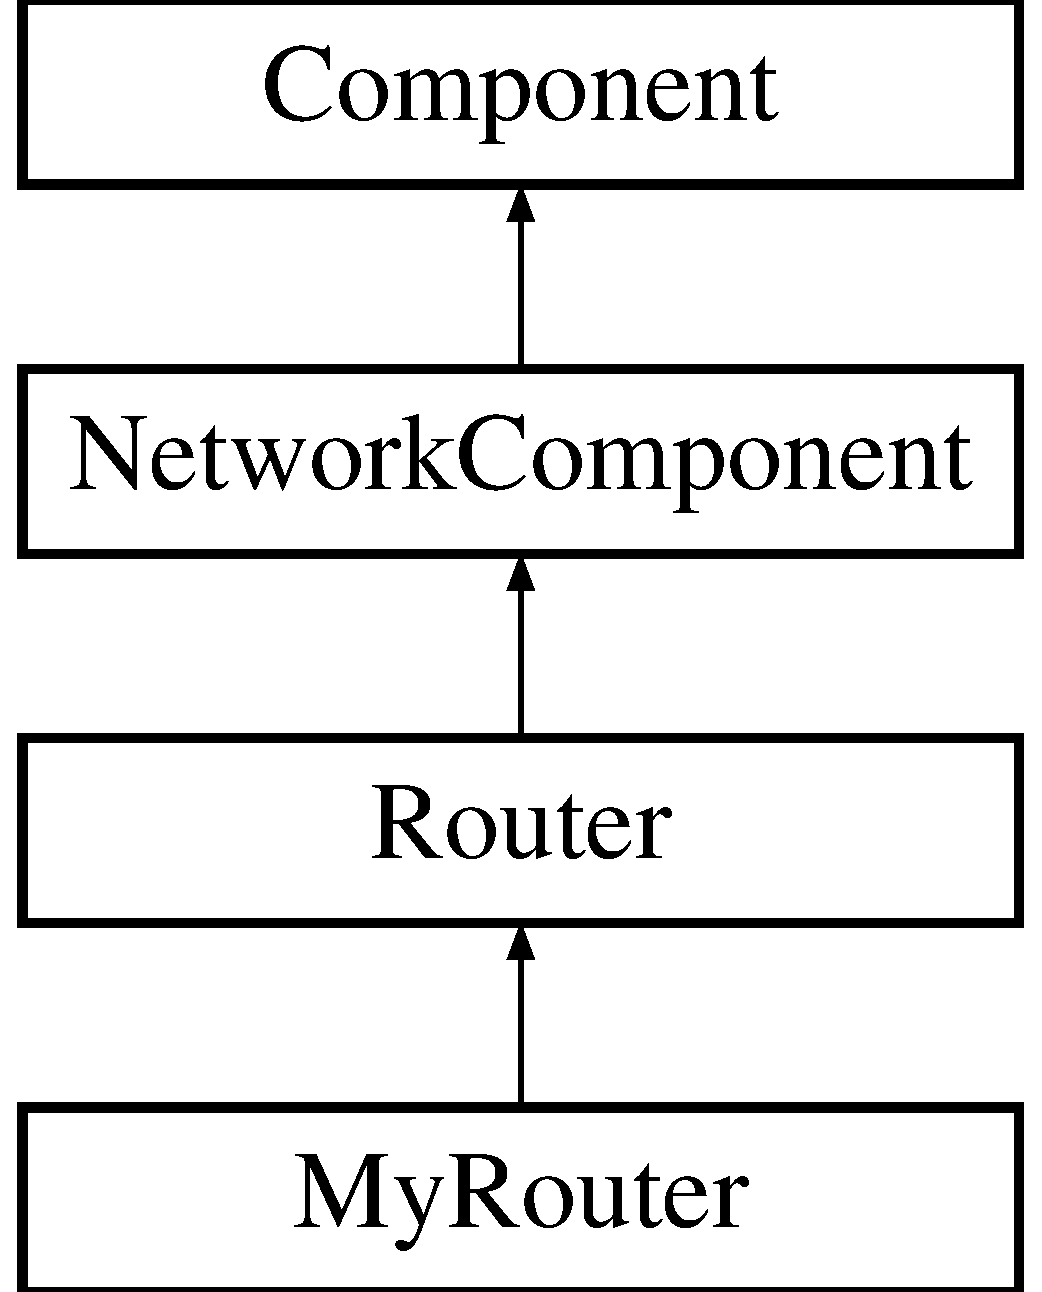
\includegraphics[height=4cm]{classMyRouter}
\end{center}
\end{figure}
\subsection*{Public Member Functions}
\begin{CompactItemize}
\item 
\hyperlink{classMyRouter_22ab97be4fbffe1aa4e33bd5cd470167}{MyRouter} ()
\item 
\hyperlink{classMyRouter_3ffe36f3427a8beeb62007909ece9dc8}{$\sim$MyRouter} ()
\item 
void \hyperlink{classMyRouter_8c9be5d944c7cb4c98f3b833e614274c}{init} ()
\item 
void \hyperlink{classMyRouter_ce1887c47f021ee3a26f678f00939bf0}{set\_\-no\_\-ports} (\hyperlink{outputBuffer_8h_91ad9478d81a7aaf2593e8d9c3d06a14}{uint} p)
\item 
void \hyperlink{classMyRouter_b7a91b2d68f0ad85e1ae3801111985c9}{set\_\-no\_\-vcs} (\hyperlink{outputBuffer_8h_91ad9478d81a7aaf2593e8d9c3d06a14}{uint} v)
\item 
void \hyperlink{classMyRouter_1136c71870bd451ac24db24612071c92}{set\_\-no\_\-credits} (int c)
\item 
void \hyperlink{classMyRouter_ee56704d0e9366dae6c26bdf90bc6343}{set\_\-buffer\_\-size} (\hyperlink{outputBuffer_8h_91ad9478d81a7aaf2593e8d9c3d06a14}{uint} b)
\item 
void \hyperlink{classMyRouter_ceb204776c6ed1fcbc0179b1d57e0ba3}{set\_\-no\_\-nodes} (\hyperlink{outputBuffer_8h_91ad9478d81a7aaf2593e8d9c3d06a14}{uint} nodes)
\item 
void \hyperlink{classMyRouter_684adfcb9dd9421f75372fe59b8ccc5f}{set\_\-grid\_\-x\_\-location} (\hyperlink{outputBuffer_8h_91ad9478d81a7aaf2593e8d9c3d06a14}{uint} a, \hyperlink{outputBuffer_8h_91ad9478d81a7aaf2593e8d9c3d06a14}{uint} b, \hyperlink{outputBuffer_8h_91ad9478d81a7aaf2593e8d9c3d06a14}{uint} c)
\item 
void \hyperlink{classMyRouter_c5edbdd2f7da6b24f941540e687706c0}{set\_\-grid\_\-y\_\-location} (\hyperlink{outputBuffer_8h_91ad9478d81a7aaf2593e8d9c3d06a14}{uint} a, \hyperlink{outputBuffer_8h_91ad9478d81a7aaf2593e8d9c3d06a14}{uint} b, \hyperlink{outputBuffer_8h_91ad9478d81a7aaf2593e8d9c3d06a14}{uint} c)
\item 
void \hyperlink{classMyRouter_bcfd73d0faaa8a191cd4ece957f3773b}{send\_\-credit\_\-back} (\hyperlink{outputBuffer_8h_91ad9478d81a7aaf2593e8d9c3d06a14}{uint} i)
\item 
void \hyperlink{classMyRouter_5dcfef46ad281c05de8e8c1bdf236a4a}{process\_\-event} (\hyperlink{classIrisEvent}{IrisEvent} $\ast$e)
\item 
string \hyperlink{classMyRouter_9b40e1d62a4638fb84f31aff143d970d}{toString} () const 
\item 
string \hyperlink{classMyRouter_ce28b171a1f2f93fa96f9d6a65fadbbe}{print\_\-stats} ()
\end{CompactItemize}
\subsection*{Public Attributes}
\begin{CompactItemize}
\item 
vector$<$ vector$<$ \hyperlink{outputBuffer_8h_91ad9478d81a7aaf2593e8d9c3d06a14}{uint} $>$ $>$ \hyperlink{classMyRouter_f15a834dbd27a5070e1b0388c2a40d4c}{downstream\_\-credits}
\item 
\hyperlink{outputBuffer_8h_91ad9478d81a7aaf2593e8d9c3d06a14}{uint} \hyperlink{classMyRouter_32ec6983b42b6efc05af4de71055eac4}{packets}
\item 
\hyperlink{outputBuffer_8h_91ad9478d81a7aaf2593e8d9c3d06a14}{uint} \hyperlink{classMyRouter_a6cc2fffa1841027970fcdb3c948781e}{flits}
\item 
double \hyperlink{classMyRouter_081915dc1164141104ffa6ce7dd05ac5}{total\_\-packet\_\-latency}
\item 
double \hyperlink{classMyRouter_1b75d62cb9e51e8814704582d787b3ec}{last\_\-flit\_\-out\_\-cycle}
\end{CompactItemize}


\subsection{Constructor \& Destructor Documentation}
\hypertarget{classMyRouter_22ab97be4fbffe1aa4e33bd5cd470167}{
\index{MyRouter@{MyRouter}!MyRouter@{MyRouter}}
\index{MyRouter@{MyRouter}!MyRouter@{MyRouter}}
\subsubsection[{MyRouter}]{\setlength{\rightskip}{0pt plus 5cm}MyRouter::MyRouter ()}}
\label{classMyRouter_22ab97be4fbffe1aa4e33bd5cd470167}


\hypertarget{classMyRouter_3ffe36f3427a8beeb62007909ece9dc8}{
\index{MyRouter@{MyRouter}!$\sim$MyRouter@{$\sim$MyRouter}}
\index{$\sim$MyRouter@{$\sim$MyRouter}!MyRouter@{MyRouter}}
\subsubsection[{$\sim$MyRouter}]{\setlength{\rightskip}{0pt plus 5cm}MyRouter::$\sim$MyRouter ()}}
\label{classMyRouter_3ffe36f3427a8beeb62007909ece9dc8}




\subsection{Member Function Documentation}
\hypertarget{classMyRouter_8c9be5d944c7cb4c98f3b833e614274c}{
\index{MyRouter@{MyRouter}!init@{init}}
\index{init@{init}!MyRouter@{MyRouter}}
\subsubsection[{init}]{\setlength{\rightskip}{0pt plus 5cm}void MyRouter::init ()}}
\label{classMyRouter_8c9be5d944c7cb4c98f3b833e614274c}


\hypertarget{classMyRouter_ce28b171a1f2f93fa96f9d6a65fadbbe}{
\index{MyRouter@{MyRouter}!print\_\-stats@{print\_\-stats}}
\index{print\_\-stats@{print\_\-stats}!MyRouter@{MyRouter}}
\subsubsection[{print\_\-stats}]{\setlength{\rightskip}{0pt plus 5cm}string MyRouter::print\_\-stats ()\hspace{0.3cm}{\tt  \mbox{[}virtual\mbox{]}}}}
\label{classMyRouter_ce28b171a1f2f93fa96f9d6a65fadbbe}




Implements \hyperlink{classRouter_75995624d8bd533a9d3eb8c06a62ce07}{Router}.\hypertarget{classMyRouter_5dcfef46ad281c05de8e8c1bdf236a4a}{
\index{MyRouter@{MyRouter}!process\_\-event@{process\_\-event}}
\index{process\_\-event@{process\_\-event}!MyRouter@{MyRouter}}
\subsubsection[{process\_\-event}]{\setlength{\rightskip}{0pt plus 5cm}void MyRouter::process\_\-event ({\bf IrisEvent} $\ast$ {\em e})\hspace{0.3cm}{\tt  \mbox{[}virtual\mbox{]}}}}
\label{classMyRouter_5dcfef46ad281c05de8e8c1bdf236a4a}




Implements \hyperlink{classNetworkComponent_c93793eea1e2d424abe86e110ca8b399}{NetworkComponent}.\hypertarget{classMyRouter_bcfd73d0faaa8a191cd4ece957f3773b}{
\index{MyRouter@{MyRouter}!send\_\-credit\_\-back@{send\_\-credit\_\-back}}
\index{send\_\-credit\_\-back@{send\_\-credit\_\-back}!MyRouter@{MyRouter}}
\subsubsection[{send\_\-credit\_\-back}]{\setlength{\rightskip}{0pt plus 5cm}void MyRouter::send\_\-credit\_\-back ({\bf uint} {\em i})}}
\label{classMyRouter_bcfd73d0faaa8a191cd4ece957f3773b}


\hypertarget{classMyRouter_ee56704d0e9366dae6c26bdf90bc6343}{
\index{MyRouter@{MyRouter}!set\_\-buffer\_\-size@{set\_\-buffer\_\-size}}
\index{set\_\-buffer\_\-size@{set\_\-buffer\_\-size}!MyRouter@{MyRouter}}
\subsubsection[{set\_\-buffer\_\-size}]{\setlength{\rightskip}{0pt plus 5cm}void MyRouter::set\_\-buffer\_\-size ({\bf uint} {\em b})}}
\label{classMyRouter_ee56704d0e9366dae6c26bdf90bc6343}


\hypertarget{classMyRouter_684adfcb9dd9421f75372fe59b8ccc5f}{
\index{MyRouter@{MyRouter}!set\_\-grid\_\-x\_\-location@{set\_\-grid\_\-x\_\-location}}
\index{set\_\-grid\_\-x\_\-location@{set\_\-grid\_\-x\_\-location}!MyRouter@{MyRouter}}
\subsubsection[{set\_\-grid\_\-x\_\-location}]{\setlength{\rightskip}{0pt plus 5cm}void MyRouter::set\_\-grid\_\-x\_\-location ({\bf uint} {\em a}, \/  {\bf uint} {\em b}, \/  {\bf uint} {\em c})}}
\label{classMyRouter_684adfcb9dd9421f75372fe59b8ccc5f}


\hypertarget{classMyRouter_c5edbdd2f7da6b24f941540e687706c0}{
\index{MyRouter@{MyRouter}!set\_\-grid\_\-y\_\-location@{set\_\-grid\_\-y\_\-location}}
\index{set\_\-grid\_\-y\_\-location@{set\_\-grid\_\-y\_\-location}!MyRouter@{MyRouter}}
\subsubsection[{set\_\-grid\_\-y\_\-location}]{\setlength{\rightskip}{0pt plus 5cm}void MyRouter::set\_\-grid\_\-y\_\-location ({\bf uint} {\em a}, \/  {\bf uint} {\em b}, \/  {\bf uint} {\em c})}}
\label{classMyRouter_c5edbdd2f7da6b24f941540e687706c0}


\hypertarget{classMyRouter_1136c71870bd451ac24db24612071c92}{
\index{MyRouter@{MyRouter}!set\_\-no\_\-credits@{set\_\-no\_\-credits}}
\index{set\_\-no\_\-credits@{set\_\-no\_\-credits}!MyRouter@{MyRouter}}
\subsubsection[{set\_\-no\_\-credits}]{\setlength{\rightskip}{0pt plus 5cm}void MyRouter::set\_\-no\_\-credits (int {\em c})}}
\label{classMyRouter_1136c71870bd451ac24db24612071c92}


\hypertarget{classMyRouter_ceb204776c6ed1fcbc0179b1d57e0ba3}{
\index{MyRouter@{MyRouter}!set\_\-no\_\-nodes@{set\_\-no\_\-nodes}}
\index{set\_\-no\_\-nodes@{set\_\-no\_\-nodes}!MyRouter@{MyRouter}}
\subsubsection[{set\_\-no\_\-nodes}]{\setlength{\rightskip}{0pt plus 5cm}void MyRouter::set\_\-no\_\-nodes ({\bf uint} {\em nodes})\hspace{0.3cm}{\tt  \mbox{[}virtual\mbox{]}}}}
\label{classMyRouter_ceb204776c6ed1fcbc0179b1d57e0ba3}




Implements \hyperlink{classRouter_33073537e883e8bea1a25690bcb70049}{Router}.\hypertarget{classMyRouter_ce1887c47f021ee3a26f678f00939bf0}{
\index{MyRouter@{MyRouter}!set\_\-no\_\-ports@{set\_\-no\_\-ports}}
\index{set\_\-no\_\-ports@{set\_\-no\_\-ports}!MyRouter@{MyRouter}}
\subsubsection[{set\_\-no\_\-ports}]{\setlength{\rightskip}{0pt plus 5cm}void MyRouter::set\_\-no\_\-ports ({\bf uint} {\em p})}}
\label{classMyRouter_ce1887c47f021ee3a26f678f00939bf0}


\hypertarget{classMyRouter_b7a91b2d68f0ad85e1ae3801111985c9}{
\index{MyRouter@{MyRouter}!set\_\-no\_\-vcs@{set\_\-no\_\-vcs}}
\index{set\_\-no\_\-vcs@{set\_\-no\_\-vcs}!MyRouter@{MyRouter}}
\subsubsection[{set\_\-no\_\-vcs}]{\setlength{\rightskip}{0pt plus 5cm}void MyRouter::set\_\-no\_\-vcs ({\bf uint} {\em v})}}
\label{classMyRouter_b7a91b2d68f0ad85e1ae3801111985c9}


\hypertarget{classMyRouter_9b40e1d62a4638fb84f31aff143d970d}{
\index{MyRouter@{MyRouter}!toString@{toString}}
\index{toString@{toString}!MyRouter@{MyRouter}}
\subsubsection[{toString}]{\setlength{\rightskip}{0pt plus 5cm}string MyRouter::toString () const\hspace{0.3cm}{\tt  \mbox{[}virtual\mbox{]}}}}
\label{classMyRouter_9b40e1d62a4638fb84f31aff143d970d}




Reimplemented from \hyperlink{classRouter_1e749a51dcf6cbd6925ac677473c7f58}{Router}.

\subsection{Member Data Documentation}
\hypertarget{classMyRouter_f15a834dbd27a5070e1b0388c2a40d4c}{
\index{MyRouter@{MyRouter}!downstream\_\-credits@{downstream\_\-credits}}
\index{downstream\_\-credits@{downstream\_\-credits}!MyRouter@{MyRouter}}
\subsubsection[{downstream\_\-credits}]{\setlength{\rightskip}{0pt plus 5cm}vector$<$ vector$<${\bf uint}$>$ $>$ {\bf MyRouter::downstream\_\-credits}}}
\label{classMyRouter_f15a834dbd27a5070e1b0388c2a40d4c}


\hypertarget{classMyRouter_a6cc2fffa1841027970fcdb3c948781e}{
\index{MyRouter@{MyRouter}!flits@{flits}}
\index{flits@{flits}!MyRouter@{MyRouter}}
\subsubsection[{flits}]{\setlength{\rightskip}{0pt plus 5cm}{\bf uint} {\bf MyRouter::flits}}}
\label{classMyRouter_a6cc2fffa1841027970fcdb3c948781e}


\hypertarget{classMyRouter_1b75d62cb9e51e8814704582d787b3ec}{
\index{MyRouter@{MyRouter}!last\_\-flit\_\-out\_\-cycle@{last\_\-flit\_\-out\_\-cycle}}
\index{last\_\-flit\_\-out\_\-cycle@{last\_\-flit\_\-out\_\-cycle}!MyRouter@{MyRouter}}
\subsubsection[{last\_\-flit\_\-out\_\-cycle}]{\setlength{\rightskip}{0pt plus 5cm}double {\bf MyRouter::last\_\-flit\_\-out\_\-cycle}}}
\label{classMyRouter_1b75d62cb9e51e8814704582d787b3ec}


\hypertarget{classMyRouter_32ec6983b42b6efc05af4de71055eac4}{
\index{MyRouter@{MyRouter}!packets@{packets}}
\index{packets@{packets}!MyRouter@{MyRouter}}
\subsubsection[{packets}]{\setlength{\rightskip}{0pt plus 5cm}{\bf uint} {\bf MyRouter::packets}}}
\label{classMyRouter_32ec6983b42b6efc05af4de71055eac4}


\hypertarget{classMyRouter_081915dc1164141104ffa6ce7dd05ac5}{
\index{MyRouter@{MyRouter}!total\_\-packet\_\-latency@{total\_\-packet\_\-latency}}
\index{total\_\-packet\_\-latency@{total\_\-packet\_\-latency}!MyRouter@{MyRouter}}
\subsubsection[{total\_\-packet\_\-latency}]{\setlength{\rightskip}{0pt plus 5cm}double {\bf MyRouter::total\_\-packet\_\-latency}}}
\label{classMyRouter_081915dc1164141104ffa6ce7dd05ac5}




The documentation for this class was generated from the following files:\begin{CompactItemize}
\item 
source/components/none/\hyperlink{myRouter_8h}{myRouter.h}\item 
source/components/none/\hyperlink{myRouter_8cc}{myRouter.cc}\end{CompactItemize}

\hypertarget{classNetworkComponent}{
\section{NetworkComponent Class Reference}
\label{classNetworkComponent}\index{NetworkComponent@{NetworkComponent}}
}
{\tt \#include $<$networkComponent.h$>$}

Inheritance diagram for NetworkComponent::\begin{figure}[H]
\begin{center}
\leavevmode
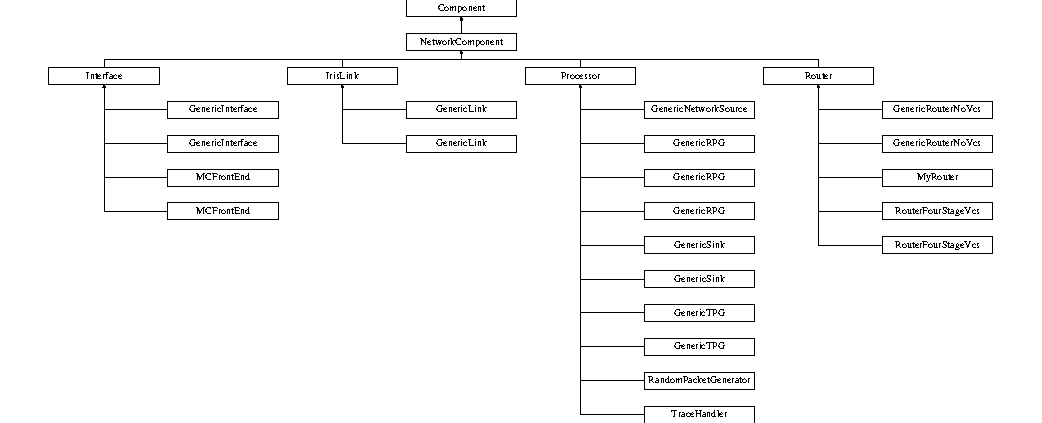
\includegraphics[height=5.6875cm]{classNetworkComponent}
\end{center}
\end{figure}
\subsection*{Public Types}
\begin{CompactItemize}
\item 
enum \hyperlink{classNetworkComponent_de3a046109ffaae8ea087feaf879b331}{types} \{ \hyperlink{classNetworkComponent_de3a046109ffaae8ea087feaf879b3310af6940aa4e653f8c152d92670a4370c}{processor}, 
\hyperlink{classNetworkComponent_de3a046109ffaae8ea087feaf879b331a5fd9b1f5cc536ac79e394578ed0a9f1}{interface}, 
\hyperlink{classNetworkComponent_de3a046109ffaae8ea087feaf879b331380174d2fb34d464f89e0f470b33102a}{link}, 
\hyperlink{classNetworkComponent_de3a046109ffaae8ea087feaf879b3318f51c4a212c73a9b847767591aa7828e}{router}
 \}
\subsection*{Public Member Functions}
\begin{CompactItemize}
\item 
\hyperlink{classNetworkComponent_fbc5367d657f132a271f4e48c1523790}{NetworkComponent} ()
\item 
virtual \hyperlink{classNetworkComponent_05adbdf1cb3611bbfd937887065d3feb}{$\sim$NetworkComponent} ()
\item 
virtual string \hyperlink{classNetworkComponent_9bb9874e1f5705588cb3d9c201d8fc6f}{toString} () const 
\item 
virtual void \hyperlink{classNetworkComponent_c93793eea1e2d424abe86e110ca8b399}{process\_\-event} (\hyperlink{classIrisEvent}{IrisEvent} $\ast$e)=0
\end{CompactItemize}
\subsection*{Public Attributes}
\begin{CompactItemize}
\item 
\hyperlink{classNetworkComponent_de3a046109ffaae8ea087feaf879b331}{types} \hyperlink{classNetworkComponent_702663f5fd8d99b8a62449a1106e0ed6}{type}
\item 
string \hyperlink{classNetworkComponent_377732efece6236958869713b6f30044}{name}
\item 
\hyperlink{ringSim_8cc_880960a57c549f69d77cf01237366978}{uniqueId} \hyperlink{classNetworkComponent_0428749bde908497630b506071d52191}{address}
\item 
\hyperlink{outputBuffer_8h_91ad9478d81a7aaf2593e8d9c3d06a14}{uint} \hyperlink{classNetworkComponent_56599b3484333fb78af1b6c33f77cf16}{node\_\-ip}
\end{CompactItemize}


\subsection{Member Enumeration Documentation}
\hypertarget{classNetworkComponent_de3a046109ffaae8ea087feaf879b331}{
\index{NetworkComponent@{NetworkComponent}!types@{types}}
\index{types@{types}!NetworkComponent@{NetworkComponent}}
\subsubsection[{types}]{\setlength{\rightskip}{0pt plus 5cm}enum {\bf NetworkComponent::types}}}
\label{classNetworkComponent_de3a046109ffaae8ea087feaf879b331}


\begin{Desc}
\item[Enumerator: ]\par
\begin{description}
\index{processor@{processor}!NetworkComponent@{NetworkComponent}}\index{NetworkComponent@{NetworkComponent}!processor@{processor}}\item[{\em 
\hypertarget{classNetworkComponent_de3a046109ffaae8ea087feaf879b3310af6940aa4e653f8c152d92670a4370c}{
processor}
\label{classNetworkComponent_de3a046109ffaae8ea087feaf879b3310af6940aa4e653f8c152d92670a4370c}
}]\index{interface@{interface}!NetworkComponent@{NetworkComponent}}\index{NetworkComponent@{NetworkComponent}!interface@{interface}}\item[{\em 
\hypertarget{classNetworkComponent_de3a046109ffaae8ea087feaf879b331a5fd9b1f5cc536ac79e394578ed0a9f1}{
interface}
\label{classNetworkComponent_de3a046109ffaae8ea087feaf879b331a5fd9b1f5cc536ac79e394578ed0a9f1}
}]\index{link@{link}!NetworkComponent@{NetworkComponent}}\index{NetworkComponent@{NetworkComponent}!link@{link}}\item[{\em 
\hypertarget{classNetworkComponent_de3a046109ffaae8ea087feaf879b331380174d2fb34d464f89e0f470b33102a}{
link}
\label{classNetworkComponent_de3a046109ffaae8ea087feaf879b331380174d2fb34d464f89e0f470b33102a}
}]\index{router@{router}!NetworkComponent@{NetworkComponent}}\index{NetworkComponent@{NetworkComponent}!router@{router}}\item[{\em 
\hypertarget{classNetworkComponent_de3a046109ffaae8ea087feaf879b3318f51c4a212c73a9b847767591aa7828e}{
router}
\label{classNetworkComponent_de3a046109ffaae8ea087feaf879b3318f51c4a212c73a9b847767591aa7828e}
}]\end{description}
\end{Desc}



\subsection{Constructor \& Destructor Documentation}
\hypertarget{classNetworkComponent_fbc5367d657f132a271f4e48c1523790}{
\index{NetworkComponent@{NetworkComponent}!NetworkComponent@{NetworkComponent}}
\index{NetworkComponent@{NetworkComponent}!NetworkComponent@{NetworkComponent}}
\subsubsection[{NetworkComponent}]{\setlength{\rightskip}{0pt plus 5cm}NetworkComponent::NetworkComponent ()}}
\label{classNetworkComponent_fbc5367d657f132a271f4e48c1523790}


\hypertarget{classNetworkComponent_05adbdf1cb3611bbfd937887065d3feb}{
\index{NetworkComponent@{NetworkComponent}!$\sim$NetworkComponent@{$\sim$NetworkComponent}}
\index{$\sim$NetworkComponent@{$\sim$NetworkComponent}!NetworkComponent@{NetworkComponent}}
\subsubsection[{$\sim$NetworkComponent}]{\setlength{\rightskip}{0pt plus 5cm}NetworkComponent::$\sim$NetworkComponent ()\hspace{0.3cm}{\tt  \mbox{[}virtual\mbox{]}}}}
\label{classNetworkComponent_05adbdf1cb3611bbfd937887065d3feb}




\subsection{Member Function Documentation}
\hypertarget{classNetworkComponent_c93793eea1e2d424abe86e110ca8b399}{
\index{NetworkComponent@{NetworkComponent}!process\_\-event@{process\_\-event}}
\index{process\_\-event@{process\_\-event}!NetworkComponent@{NetworkComponent}}
\subsubsection[{process\_\-event}]{\setlength{\rightskip}{0pt plus 5cm}virtual void NetworkComponent::process\_\-event ({\bf IrisEvent} $\ast$ {\em e})\hspace{0.3cm}{\tt  \mbox{[}pure virtual\mbox{]}}}}
\label{classNetworkComponent_c93793eea1e2d424abe86e110ca8b399}




Implemented in \hyperlink{classGenericRouterNoVcs_a2c52d53e127c9a3a029194e77f9f80c}{GenericRouterNoVcs}, \hyperlink{classGenericRPG_72d08c87beeb16514c6c81af3296f6af}{GenericRPG}, \hyperlink{classMCFrontEnd_cc935494693a9b02addf8ea8c04f81b3}{MCFrontEnd}, \hyperlink{classRouterFourStageVcs_81562fa747c216e200476ab1f85699bf}{RouterFourStageVcs}, \hyperlink{classGenericInterface_d56b8876204889d3c096fccd61b16b9e}{GenericInterface}, \hyperlink{classGenericLink_c09533f8445eb3c550c744fd4ada7324}{GenericLink}, \hyperlink{classGenericRouterNoVcs_a2c52d53e127c9a3a029194e77f9f80c}{GenericRouterNoVcs}, \hyperlink{classGenericRPG_72d08c87beeb16514c6c81af3296f6af}{GenericRPG}, \hyperlink{classGenericSink_a0beb58f52adfe869ba47f4b51537409}{GenericSink}, \hyperlink{classGenericTPG_a2e59f102384206268808835bcb9d5b5}{GenericTPG}, \hyperlink{classInterface_baaaeb823b1e0fd7ddc1bb32c2f016fb}{Interface}, \hyperlink{classIrisLink_9c5494bc5716aedf3affe748f3a542c1}{IrisLink}, \hyperlink{classProcessor_18cdeefafbd8225cb3ad18dd098c0e08}{Processor}, \hyperlink{classGenericInterface_d56b8876204889d3c096fccd61b16b9e}{GenericInterface}, \hyperlink{classGenericLink_c09533f8445eb3c550c744fd4ada7324}{GenericLink}, \hyperlink{classGenericRPG_72d08c87beeb16514c6c81af3296f6af}{GenericRPG}, \hyperlink{classGenericSink_a0beb58f52adfe869ba47f4b51537409}{GenericSink}, \hyperlink{classGenericTPG_a2e59f102384206268808835bcb9d5b5}{GenericTPG}, \hyperlink{classMCFrontEnd_cc935494693a9b02addf8ea8c04f81b3}{MCFrontEnd}, \hyperlink{classMyRouter_5dcfef46ad281c05de8e8c1bdf236a4a}{MyRouter}, \hyperlink{classRouterFourStageVcs_81562fa747c216e200476ab1f85699bf}{RouterFourStageVcs}, \hyperlink{classGenericNetworkSource_a67be5ac0f97b7e0b38eba909cecaa64}{GenericNetworkSource}, \hyperlink{classRandomPacketGenerator_127a1f17b384e0418f055b0c22eb925a}{RandomPacketGenerator}, and \hyperlink{classTraceHandler_ce34c9fd6ca6893af23d1167348ee0c9}{TraceHandler}.\hypertarget{classNetworkComponent_9bb9874e1f5705588cb3d9c201d8fc6f}{
\index{NetworkComponent@{NetworkComponent}!toString@{toString}}
\index{toString@{toString}!NetworkComponent@{NetworkComponent}}
\subsubsection[{toString}]{\setlength{\rightskip}{0pt plus 5cm}string NetworkComponent::toString () const\hspace{0.3cm}{\tt  \mbox{[}virtual\mbox{]}}}}
\label{classNetworkComponent_9bb9874e1f5705588cb3d9c201d8fc6f}




Reimplemented in \hyperlink{classGenericRouterNoVcs_59307c319fbca5732d750630be9ee27c}{GenericRouterNoVcs}, \hyperlink{classGenericRPG_a4303867728559ab6e6ae3d1390ede71}{GenericRPG}, \hyperlink{classMCFrontEnd_9dda980a7ae732e6cb6da7121bc4f539}{MCFrontEnd}, \hyperlink{classRouterFourStageVcs_0f2d0c3bcd780832ec371374eb3950fd}{RouterFourStageVcs}, \hyperlink{classGenericInterface_ae1400fce0c7ba48965596ec172e474b}{GenericInterface}, \hyperlink{classGenericLink_64dad2c98848fb48b3b572887031167b}{GenericLink}, \hyperlink{classGenericRouterNoVcs_59307c319fbca5732d750630be9ee27c}{GenericRouterNoVcs}, \hyperlink{classGenericRPG_a4303867728559ab6e6ae3d1390ede71}{GenericRPG}, \hyperlink{classGenericSink_a1703a08208816130a4ee2f4d4a8334f}{GenericSink}, \hyperlink{classGenericTPG_c2e1dc7b0de824c846f37c4a1c282303}{GenericTPG}, \hyperlink{classInterface_137cdb3bca46eb2ae0bbf017d1efb66e}{Interface}, \hyperlink{classIrisLink_d25db1c98385d7abd82180e5746813a6}{IrisLink}, \hyperlink{classProcessor_d3bdbedfbb00b05f61504e411a418106}{Processor}, \hyperlink{classRouter_1e749a51dcf6cbd6925ac677473c7f58}{Router}, \hyperlink{classGenericInterface_ae1400fce0c7ba48965596ec172e474b}{GenericInterface}, \hyperlink{classGenericLink_64dad2c98848fb48b3b572887031167b}{GenericLink}, \hyperlink{classGenericRPG_a4303867728559ab6e6ae3d1390ede71}{GenericRPG}, \hyperlink{classGenericSink_a1703a08208816130a4ee2f4d4a8334f}{GenericSink}, \hyperlink{classGenericTPG_c2e1dc7b0de824c846f37c4a1c282303}{GenericTPG}, \hyperlink{classMCFrontEnd_9dda980a7ae732e6cb6da7121bc4f539}{MCFrontEnd}, \hyperlink{classMyRouter_9b40e1d62a4638fb84f31aff143d970d}{MyRouter}, \hyperlink{classRouterFourStageVcs_0f2d0c3bcd780832ec371374eb3950fd}{RouterFourStageVcs}, \hyperlink{classGenericNetworkSource_8d8c0760eb634da3ccc3d4083e9415b9}{GenericNetworkSource}, \hyperlink{classRandomPacketGenerator_4031f11000db9e2693c761f7f47a4c88}{RandomPacketGenerator}, and \hyperlink{classTraceHandler_e2a56abded1637aba10677483fee4e32}{TraceHandler}.

\subsection{Member Data Documentation}
\hypertarget{classNetworkComponent_0428749bde908497630b506071d52191}{
\index{NetworkComponent@{NetworkComponent}!address@{address}}
\index{address@{address}!NetworkComponent@{NetworkComponent}}
\subsubsection[{address}]{\setlength{\rightskip}{0pt plus 5cm}{\bf uniqueId} {\bf NetworkComponent::address}}}
\label{classNetworkComponent_0428749bde908497630b506071d52191}




Reimplemented in \hyperlink{classGenericRPG_12a401de0099f5d1e2486886d3a99f0f}{GenericRPG}, \hyperlink{classGenericSink_ccb1d47a4bec1322b3e8c996933e4aaf}{GenericSink}, \hyperlink{classRandomPacketGenerator_b173df66cb0c2f96937e8e71319a510e}{RandomPacketGenerator}, and \hyperlink{classTraceHandler_ea33725c91bfe1fa432e76eade7712ed}{TraceHandler}.\hypertarget{classNetworkComponent_377732efece6236958869713b6f30044}{
\index{NetworkComponent@{NetworkComponent}!name@{name}}
\index{name@{name}!NetworkComponent@{NetworkComponent}}
\subsubsection[{name}]{\setlength{\rightskip}{0pt plus 5cm}string {\bf NetworkComponent::name}}}
\label{classNetworkComponent_377732efece6236958869713b6f30044}


\hypertarget{classNetworkComponent_56599b3484333fb78af1b6c33f77cf16}{
\index{NetworkComponent@{NetworkComponent}!node\_\-ip@{node\_\-ip}}
\index{node\_\-ip@{node\_\-ip}!NetworkComponent@{NetworkComponent}}
\subsubsection[{node\_\-ip}]{\setlength{\rightskip}{0pt plus 5cm}{\bf uint} {\bf NetworkComponent::node\_\-ip}}}
\label{classNetworkComponent_56599b3484333fb78af1b6c33f77cf16}




Reimplemented in \hyperlink{classMCFrontEnd_99eed4a2a554a84018c06637e863b525}{MCFrontEnd}, \hyperlink{classGenericNetworkSource_90d400349086508bb6b2b46fbd24ed9b}{GenericNetworkSource}, \hyperlink{classRandomPacketGenerator_072334e770d2a5a5ee77c7a859fad16b}{RandomPacketGenerator}, and \hyperlink{classTraceHandler_b54df7fbf5273b6132975f3e5bf26057}{TraceHandler}.\hypertarget{classNetworkComponent_702663f5fd8d99b8a62449a1106e0ed6}{
\index{NetworkComponent@{NetworkComponent}!type@{type}}
\index{type@{type}!NetworkComponent@{NetworkComponent}}
\subsubsection[{type}]{\setlength{\rightskip}{0pt plus 5cm}{\bf types} {\bf NetworkComponent::type}}}
\label{classNetworkComponent_702663f5fd8d99b8a62449a1106e0ed6}




The documentation for this class was generated from the following files:\begin{CompactItemize}
\item 
source/components/interfaces/\hyperlink{networkComponent_8h}{networkComponent.h}\item 
source/components/interfaces/\hyperlink{networkComponent_8cc}{networkComponent.cc}\end{CompactItemize}

\hypertarget{classNormal}{
\section{Normal Class Reference}
\label{classNormal}\index{Normal@{Normal}}
}
{\tt \#include $<$rng.hpp$>$}

Inheritance diagram for Normal::\begin{figure}[H]
\begin{center}
\leavevmode
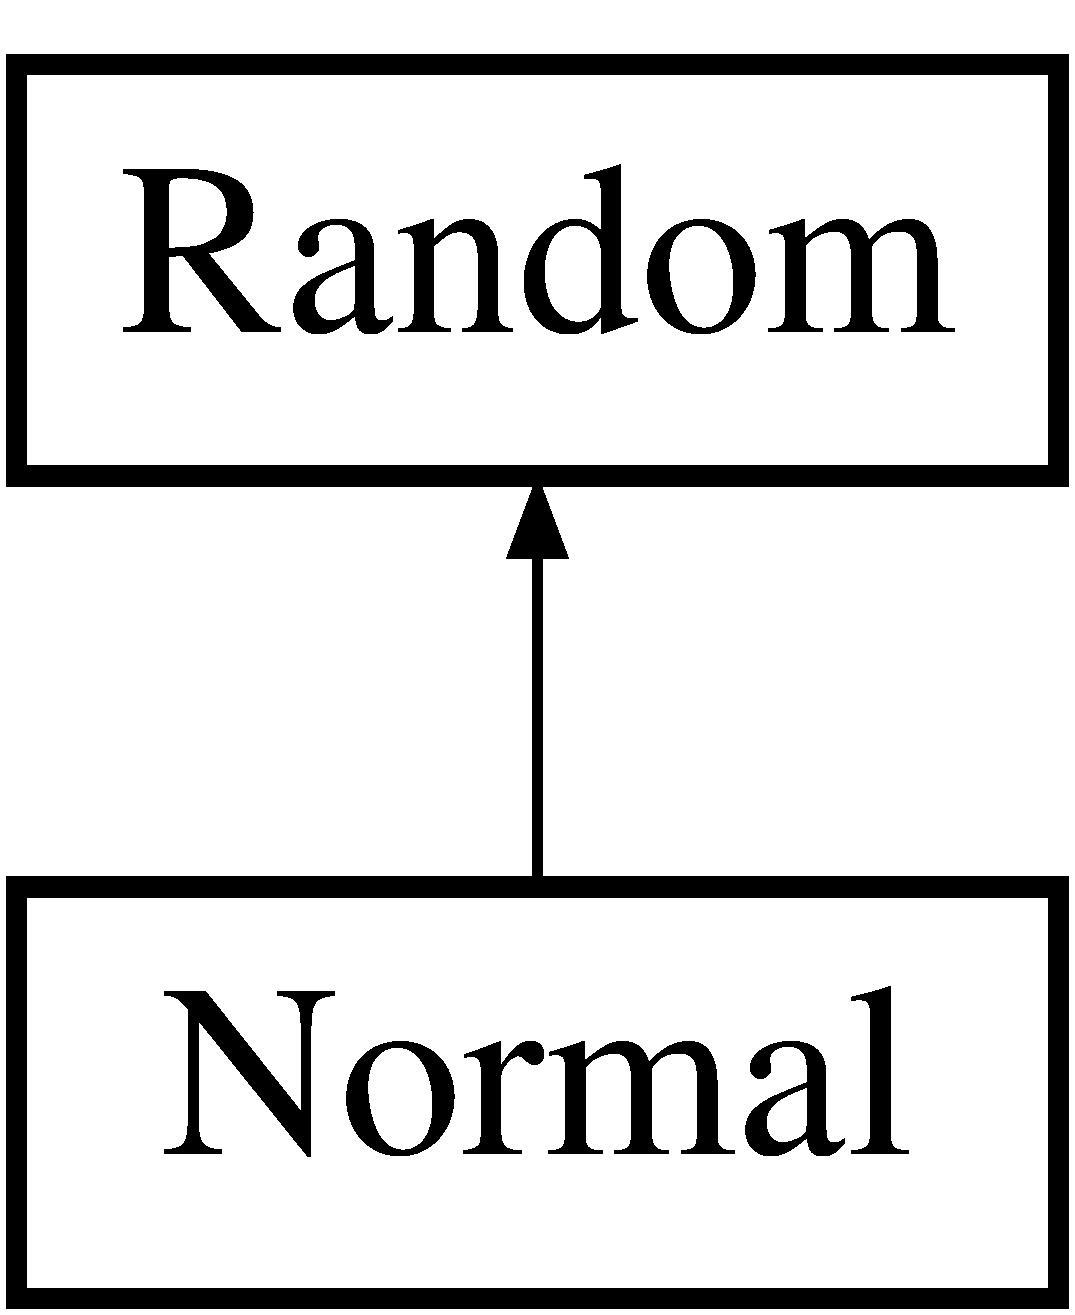
\includegraphics[height=2cm]{classNormal}
\end{center}
\end{figure}
\subsection*{Public Member Functions}
\begin{CompactItemize}
\item 
\hyperlink{classNormal_f62e51ec40dc2eedc3b9ca49ebdc7197}{Normal} ()
\item 
\hyperlink{classNormal_d217f8c08ba608aa4409f60bb7a8bb9d}{Normal} (\hyperlink{rng_8hpp_ad41e7f5d86b1109b6a6a032c86cdd3f}{Random\_\-t} m, \hyperlink{rng_8hpp_ad41e7f5d86b1109b6a6a032c86cdd3f}{Random\_\-t} v, \hyperlink{rng_8hpp_ad41e7f5d86b1109b6a6a032c86cdd3f}{Random\_\-t} b=INFINITE\_\-VALUE)
\item 
\hyperlink{classNormal_f79886344f9b8e79820d78aeb68e3e00}{Normal} (const \hyperlink{classNormal}{Normal} \&c)
\item 
virtual \hyperlink{rng_8hpp_ad41e7f5d86b1109b6a6a032c86cdd3f}{Random\_\-t} \hyperlink{classNormal_f9f5b8c8ba6dff8beb660a70935dd99e}{Value} ()
\item 
virtual \hyperlink{classRandom}{Random} $\ast$ \hyperlink{classNormal_e59f996a159efc4b26c6e373f672b050}{Copy} () const 
\end{CompactItemize}


\subsection{Constructor \& Destructor Documentation}
\hypertarget{classNormal_f62e51ec40dc2eedc3b9ca49ebdc7197}{
\index{Normal@{Normal}!Normal@{Normal}}
\index{Normal@{Normal}!Normal@{Normal}}
\subsubsection[{Normal}]{\setlength{\rightskip}{0pt plus 5cm}Normal::Normal ()\hspace{0.3cm}{\tt  \mbox{[}inline\mbox{]}}}}
\label{classNormal_f62e51ec40dc2eedc3b9ca49ebdc7197}


\hypertarget{classNormal_d217f8c08ba608aa4409f60bb7a8bb9d}{
\index{Normal@{Normal}!Normal@{Normal}}
\index{Normal@{Normal}!Normal@{Normal}}
\subsubsection[{Normal}]{\setlength{\rightskip}{0pt plus 5cm}Normal::Normal ({\bf Random\_\-t} {\em m}, \/  {\bf Random\_\-t} {\em v}, \/  {\bf Random\_\-t} {\em b} = {\tt INFINITE\_\-VALUE})\hspace{0.3cm}{\tt  \mbox{[}inline\mbox{]}}}}
\label{classNormal_d217f8c08ba608aa4409f60bb7a8bb9d}


\hypertarget{classNormal_f79886344f9b8e79820d78aeb68e3e00}{
\index{Normal@{Normal}!Normal@{Normal}}
\index{Normal@{Normal}!Normal@{Normal}}
\subsubsection[{Normal}]{\setlength{\rightskip}{0pt plus 5cm}Normal::Normal (const {\bf Normal} \& {\em c})\hspace{0.3cm}{\tt  \mbox{[}inline\mbox{]}}}}
\label{classNormal_f79886344f9b8e79820d78aeb68e3e00}




\subsection{Member Function Documentation}
\hypertarget{classNormal_e59f996a159efc4b26c6e373f672b050}{
\index{Normal@{Normal}!Copy@{Copy}}
\index{Copy@{Copy}!Normal@{Normal}}
\subsubsection[{Copy}]{\setlength{\rightskip}{0pt plus 5cm}{\bf Random} $\ast$ Normal::Copy () const\hspace{0.3cm}{\tt  \mbox{[}virtual\mbox{]}}}}
\label{classNormal_e59f996a159efc4b26c6e373f672b050}




Reimplemented from \hyperlink{classRandom_22b2951acd2008e8ff58fae434ab7ac5}{Random}.\hypertarget{classNormal_f9f5b8c8ba6dff8beb660a70935dd99e}{
\index{Normal@{Normal}!Value@{Value}}
\index{Value@{Value}!Normal@{Normal}}
\subsubsection[{Value}]{\setlength{\rightskip}{0pt plus 5cm}{\bf Random\_\-t} Normal::Value ()\hspace{0.3cm}{\tt  \mbox{[}virtual\mbox{]}}}}
\label{classNormal_f9f5b8c8ba6dff8beb660a70935dd99e}




Reimplemented from \hyperlink{classRandom_4d1c2876c5c78104186e241209d0e11e}{Random}.

The documentation for this class was generated from the following files:\begin{CompactItemize}
\item 
source/randomNumbers/impl/\hyperlink{rng_8hpp}{rng.hpp}\item 
source/randomNumbers/impl/\hyperlink{rng_8cpp}{rng.cpp}\end{CompactItemize}

\hypertarget{classOutput0}{
\section{Output0$<$ OBJ $>$ Class Template Reference}
\label{classOutput0}\index{Output0@{Output0}}
}
{\tt \#include $<$link.h$>$}

Inheritance diagram for Output0$<$ OBJ $>$::\begin{figure}[H]
\begin{center}
\leavevmode
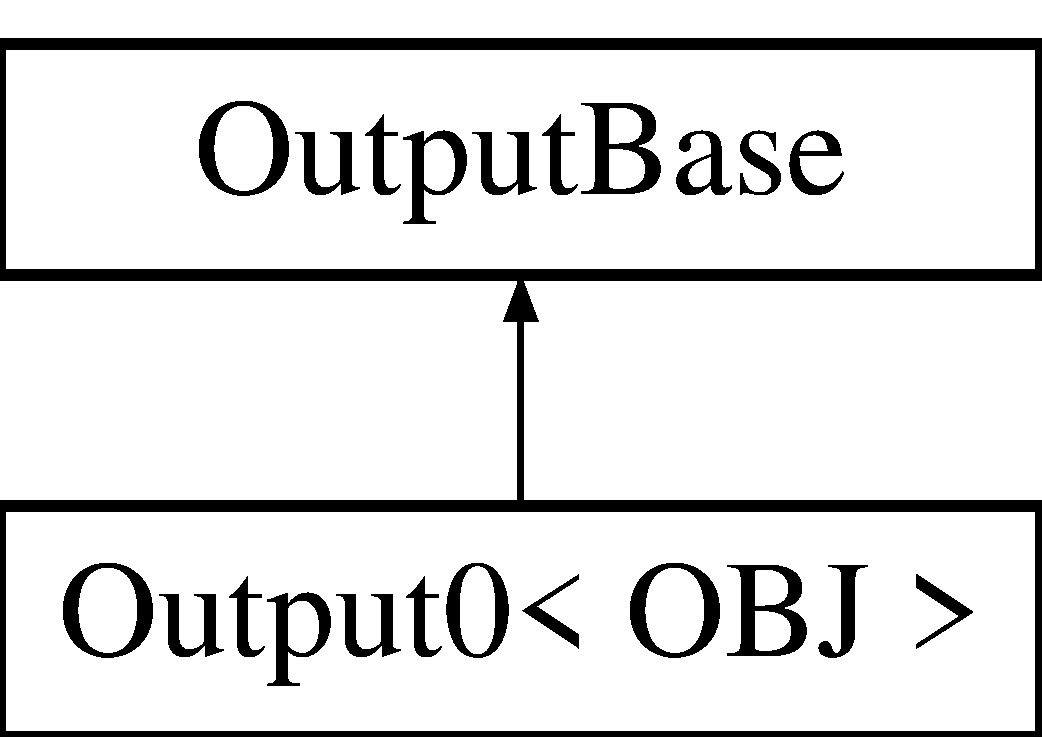
\includegraphics[height=2cm]{classOutput0}
\end{center}
\end{figure}
\subsection*{Public Member Functions}
\begin{CompactItemize}
\item 
\hyperlink{classOutput0_87632bde7780d0da8dc4fb19bf862d95}{Output0} (int \hyperlink{classOutputBase_93729601fb94bd561cb16ea2601d5528}{componentId}, double l, void(OBJ::$\ast$f)(uint64\_\-t, int), OBJ $\ast$obj0)
\item 
void \hyperlink{classOutput0_37e386a07fe2a033a847a39973458941}{CallHandler} (uint64\_\-t data, int src)
\end{CompactItemize}
\subsection*{Public Attributes}
\begin{CompactItemize}
\item 
void(OBJ::$\ast$ \hyperlink{classOutput0_3c30dd558372ba2fcbaa0748947b5161}{handler} )(uint64\_\-t, int)
\item 
OBJ $\ast$ \hyperlink{classOutput0_2dd51d5df9d69af8c45a0e7512cfbfec}{obj}
\end{CompactItemize}
\subsubsection*{template$<$typename OBJ$>$ class Output0$<$ OBJ $>$}



\subsection{Constructor \& Destructor Documentation}
\hypertarget{classOutput0_87632bde7780d0da8dc4fb19bf862d95}{
\index{Output0@{Output0}!Output0@{Output0}}
\index{Output0@{Output0}!Output0@{Output0}}
\subsubsection[{Output0}]{\setlength{\rightskip}{0pt plus 5cm}template$<$typename OBJ$>$ {\bf Output0}$<$ OBJ $>$::{\bf Output0} (int {\em componentId}, \/  double {\em l}, \/  void(OBJ::$\ast$)(uint64\_\-t, int) {\em f}, \/  OBJ $\ast$ {\em obj0})\hspace{0.3cm}{\tt  \mbox{[}inline\mbox{]}}}}
\label{classOutput0_87632bde7780d0da8dc4fb19bf862d95}




\subsection{Member Function Documentation}
\hypertarget{classOutput0_37e386a07fe2a033a847a39973458941}{
\index{Output0@{Output0}!CallHandler@{CallHandler}}
\index{CallHandler@{CallHandler}!Output0@{Output0}}
\subsubsection[{CallHandler}]{\setlength{\rightskip}{0pt plus 5cm}template$<$typename OBJ$>$ void {\bf Output0}$<$ OBJ $>$::CallHandler (uint64\_\-t {\em data}, \/  int {\em src})\hspace{0.3cm}{\tt  \mbox{[}inline, virtual\mbox{]}}}}
\label{classOutput0_37e386a07fe2a033a847a39973458941}




Implements \hyperlink{classOutputBase_2d7b62cb9883958534b55b7bfa391394}{OutputBase}.

\subsection{Member Data Documentation}
\hypertarget{classOutput0_3c30dd558372ba2fcbaa0748947b5161}{
\index{Output0@{Output0}!handler@{handler}}
\index{handler@{handler}!Output0@{Output0}}
\subsubsection[{handler}]{\setlength{\rightskip}{0pt plus 5cm}template$<$typename OBJ$>$ void(OBJ::$\ast$ {\bf Output0}$<$ OBJ $>$::{\bf handler})(uint64\_\-t, int)}}
\label{classOutput0_3c30dd558372ba2fcbaa0748947b5161}


\hypertarget{classOutput0_2dd51d5df9d69af8c45a0e7512cfbfec}{
\index{Output0@{Output0}!obj@{obj}}
\index{obj@{obj}!Output0@{Output0}}
\subsubsection[{obj}]{\setlength{\rightskip}{0pt plus 5cm}template$<$typename OBJ$>$ OBJ$\ast$ {\bf Output0}$<$ OBJ $>$::{\bf obj}}}
\label{classOutput0_2dd51d5df9d69af8c45a0e7512cfbfec}




The documentation for this class was generated from the following file:\begin{CompactItemize}
\item 
source/kernel/\hyperlink{link_8h}{link.h}\end{CompactItemize}

\hypertarget{classOutputBase}{
\section{OutputBase Class Reference}
\label{classOutputBase}\index{OutputBase@{OutputBase}}
}
{\tt \#include $<$link.h$>$}

Inheritance diagram for OutputBase::\begin{figure}[H]
\begin{center}
\leavevmode
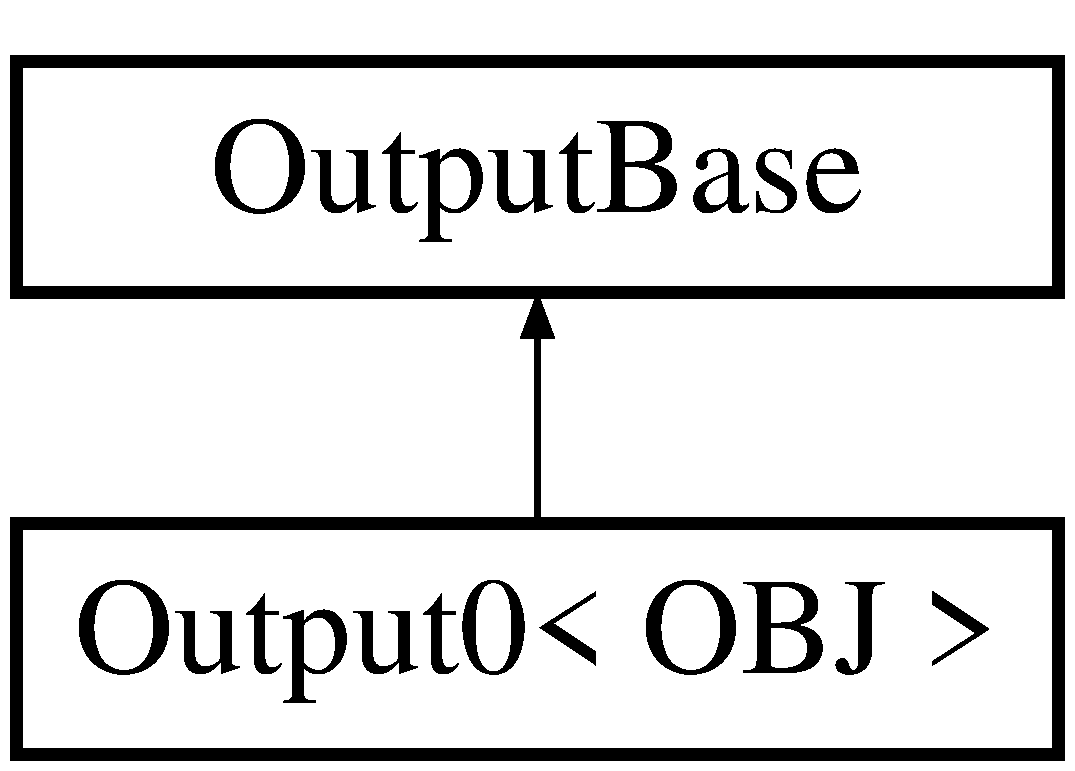
\includegraphics[height=2cm]{classOutputBase}
\end{center}
\end{figure}
\subsection*{Public Member Functions}
\begin{CompactItemize}
\item 
\hyperlink{classOutputBase_4fff2d392d52f721a8d57c51aa1ac852}{OutputBase} (int ID, double l)
\item 
virtual void \hyperlink{classOutputBase_2d7b62cb9883958534b55b7bfa391394}{CallHandler} (uint64\_\-t, int)=0
\end{CompactItemize}
\subsection*{Public Attributes}
\begin{CompactItemize}
\item 
int \hyperlink{classOutputBase_93729601fb94bd561cb16ea2601d5528}{componentId}
\item 
double \hyperlink{classOutputBase_d2e8f2c3509a16cc1ae79f1f3f89ab27}{latency}
\end{CompactItemize}


\subsection{Constructor \& Destructor Documentation}
\hypertarget{classOutputBase_4fff2d392d52f721a8d57c51aa1ac852}{
\index{OutputBase@{OutputBase}!OutputBase@{OutputBase}}
\index{OutputBase@{OutputBase}!OutputBase@{OutputBase}}
\subsubsection[{OutputBase}]{\setlength{\rightskip}{0pt plus 5cm}OutputBase::OutputBase (int {\em ID}, \/  double {\em l})\hspace{0.3cm}{\tt  \mbox{[}inline\mbox{]}}}}
\label{classOutputBase_4fff2d392d52f721a8d57c51aa1ac852}




\subsection{Member Function Documentation}
\hypertarget{classOutputBase_2d7b62cb9883958534b55b7bfa391394}{
\index{OutputBase@{OutputBase}!CallHandler@{CallHandler}}
\index{CallHandler@{CallHandler}!OutputBase@{OutputBase}}
\subsubsection[{CallHandler}]{\setlength{\rightskip}{0pt plus 5cm}virtual void OutputBase::CallHandler (uint64\_\-t, \/  int)\hspace{0.3cm}{\tt  \mbox{[}pure virtual\mbox{]}}}}
\label{classOutputBase_2d7b62cb9883958534b55b7bfa391394}




Implemented in \hyperlink{classOutput0_37e386a07fe2a033a847a39973458941}{Output0$<$ OBJ $>$}.

\subsection{Member Data Documentation}
\hypertarget{classOutputBase_93729601fb94bd561cb16ea2601d5528}{
\index{OutputBase@{OutputBase}!componentId@{componentId}}
\index{componentId@{componentId}!OutputBase@{OutputBase}}
\subsubsection[{componentId}]{\setlength{\rightskip}{0pt plus 5cm}int {\bf OutputBase::componentId}}}
\label{classOutputBase_93729601fb94bd561cb16ea2601d5528}


\hypertarget{classOutputBase_d2e8f2c3509a16cc1ae79f1f3f89ab27}{
\index{OutputBase@{OutputBase}!latency@{latency}}
\index{latency@{latency}!OutputBase@{OutputBase}}
\subsubsection[{latency}]{\setlength{\rightskip}{0pt plus 5cm}double {\bf OutputBase::latency}}}
\label{classOutputBase_d2e8f2c3509a16cc1ae79f1f3f89ab27}




The documentation for this class was generated from the following file:\begin{CompactItemize}
\item 
source/kernel/\hyperlink{link_8h}{link.h}\end{CompactItemize}

\hypertarget{classOutputBuffer}{
\section{OutputBuffer Class Reference}
\label{classOutputBuffer}\index{OutputBuffer@{OutputBuffer}}
}
{\tt \#include $<$outputBuffer.h$>$}

Inheritance diagram for OutputBuffer::\begin{figure}[H]
\begin{center}
\leavevmode
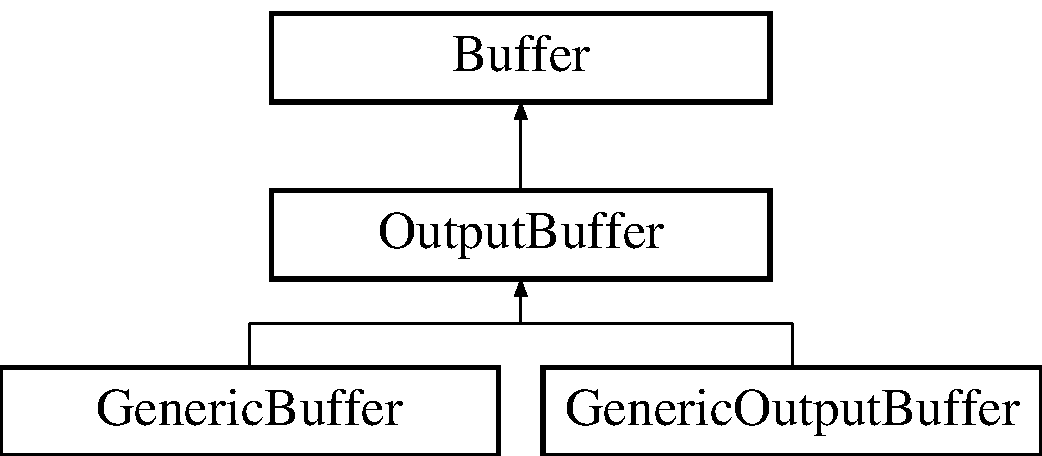
\includegraphics[height=3cm]{classOutputBuffer}
\end{center}
\end{figure}
\subsection*{Public Member Functions}
\begin{CompactItemize}
\item 
\hyperlink{classOutputBuffer_7a4352dc067a09bf7076bd7f8c6f6e1b}{OutputBuffer} ()
\item 
virtual \hyperlink{classOutputBuffer_928cc1b1e5cef13f3572c13775d547b5}{$\sim$OutputBuffer} ()
\item 
virtual void \hyperlink{classOutputBuffer_5fafb6827567941d238ae16991c5c1a8}{set\_\-no\_\-vcs} (\hyperlink{outputBuffer_8h_91ad9478d81a7aaf2593e8d9c3d06a14}{uint} number)=0
\item 
virtual \hyperlink{outputBuffer_8h_91ad9478d81a7aaf2593e8d9c3d06a14}{uint} \hyperlink{classOutputBuffer_21ad5222afd999f390df4a495eb48b0a}{get\_\-no\_\-vcs} () const =0
\item 
virtual void \hyperlink{classOutputBuffer_fb8e0a16f34dcff4c0d954201712f762}{change\_\-pull\_\-channel} (\hyperlink{outputBuffer_8h_91ad9478d81a7aaf2593e8d9c3d06a14}{uint} channel)=0
\item 
virtual void \hyperlink{classOutputBuffer_45a685173b5c5cbe6270c9e0ce6d023a}{change\_\-push\_\-channel} (\hyperlink{outputBuffer_8h_91ad9478d81a7aaf2593e8d9c3d06a14}{uint} channel)=0
\item 
virtual \hyperlink{outputBuffer_8h_91ad9478d81a7aaf2593e8d9c3d06a14}{uint} \hyperlink{classOutputBuffer_c4460c1a1ac34667c12cc77c57a393b9}{get\_\-pull\_\-channel} () const =0
\item 
virtual \hyperlink{outputBuffer_8h_91ad9478d81a7aaf2593e8d9c3d06a14}{uint} \hyperlink{classOutputBuffer_bafd65458146d9b383643fef94b38881}{get\_\-push\_\-channel} () const =0
\item 
virtual bool \hyperlink{classOutputBuffer_23aaeb2aa62e944596d50a569ed5d859}{is\_\-channel\_\-full} (\hyperlink{outputBuffer_8h_91ad9478d81a7aaf2593e8d9c3d06a14}{uint} channel) const =0
\item 
virtual bool \hyperlink{classOutputBuffer_7cba09e2dbb3794d873862b5066fd085}{is\_\-empty} (\hyperlink{outputBuffer_8h_91ad9478d81a7aaf2593e8d9c3d06a14}{uint} channel) const =0
\end{CompactItemize}


\subsection{Constructor \& Destructor Documentation}
\hypertarget{classOutputBuffer_7a4352dc067a09bf7076bd7f8c6f6e1b}{
\index{OutputBuffer@{OutputBuffer}!OutputBuffer@{OutputBuffer}}
\index{OutputBuffer@{OutputBuffer}!OutputBuffer@{OutputBuffer}}
\subsubsection[{OutputBuffer}]{\setlength{\rightskip}{0pt plus 5cm}OutputBuffer::OutputBuffer ()\hspace{0.3cm}{\tt  \mbox{[}inline\mbox{]}}}}
\label{classOutputBuffer_7a4352dc067a09bf7076bd7f8c6f6e1b}


\hypertarget{classOutputBuffer_928cc1b1e5cef13f3572c13775d547b5}{
\index{OutputBuffer@{OutputBuffer}!$\sim$OutputBuffer@{$\sim$OutputBuffer}}
\index{$\sim$OutputBuffer@{$\sim$OutputBuffer}!OutputBuffer@{OutputBuffer}}
\subsubsection[{$\sim$OutputBuffer}]{\setlength{\rightskip}{0pt plus 5cm}virtual OutputBuffer::$\sim$OutputBuffer ()\hspace{0.3cm}{\tt  \mbox{[}inline, virtual\mbox{]}}}}
\label{classOutputBuffer_928cc1b1e5cef13f3572c13775d547b5}




\subsection{Member Function Documentation}
\hypertarget{classOutputBuffer_fb8e0a16f34dcff4c0d954201712f762}{
\index{OutputBuffer@{OutputBuffer}!change\_\-pull\_\-channel@{change\_\-pull\_\-channel}}
\index{change\_\-pull\_\-channel@{change\_\-pull\_\-channel}!OutputBuffer@{OutputBuffer}}
\subsubsection[{change\_\-pull\_\-channel}]{\setlength{\rightskip}{0pt plus 5cm}virtual void OutputBuffer::change\_\-pull\_\-channel ({\bf uint} {\em channel})\hspace{0.3cm}{\tt  \mbox{[}pure virtual\mbox{]}}}}
\label{classOutputBuffer_fb8e0a16f34dcff4c0d954201712f762}




Implemented in \hyperlink{classGenericBuffer_6d7fe4a638dc7eb0358c3490bf8d2cf4}{GenericBuffer}, and \hyperlink{classGenericOutputBuffer_c4f3cf09d07b340af349820bcaed731e}{GenericOutputBuffer}.\hypertarget{classOutputBuffer_45a685173b5c5cbe6270c9e0ce6d023a}{
\index{OutputBuffer@{OutputBuffer}!change\_\-push\_\-channel@{change\_\-push\_\-channel}}
\index{change\_\-push\_\-channel@{change\_\-push\_\-channel}!OutputBuffer@{OutputBuffer}}
\subsubsection[{change\_\-push\_\-channel}]{\setlength{\rightskip}{0pt plus 5cm}virtual void OutputBuffer::change\_\-push\_\-channel ({\bf uint} {\em channel})\hspace{0.3cm}{\tt  \mbox{[}pure virtual\mbox{]}}}}
\label{classOutputBuffer_45a685173b5c5cbe6270c9e0ce6d023a}




Implemented in \hyperlink{classGenericBuffer_31e2c8b678d219fcc5d6e351f2f8623c}{GenericBuffer}, and \hyperlink{classGenericOutputBuffer_d7576df13afbc101eb997e35ad417739}{GenericOutputBuffer}.\hypertarget{classOutputBuffer_21ad5222afd999f390df4a495eb48b0a}{
\index{OutputBuffer@{OutputBuffer}!get\_\-no\_\-vcs@{get\_\-no\_\-vcs}}
\index{get\_\-no\_\-vcs@{get\_\-no\_\-vcs}!OutputBuffer@{OutputBuffer}}
\subsubsection[{get\_\-no\_\-vcs}]{\setlength{\rightskip}{0pt plus 5cm}virtual {\bf uint} OutputBuffer::get\_\-no\_\-vcs () const\hspace{0.3cm}{\tt  \mbox{[}pure virtual\mbox{]}}}}
\label{classOutputBuffer_21ad5222afd999f390df4a495eb48b0a}




Implemented in \hyperlink{classGenericBuffer_528c7b73ffbb3870cab0fc999a01a024}{GenericBuffer}, and \hyperlink{classGenericOutputBuffer_6f5495e1ddd1b524d105d86b083e85cc}{GenericOutputBuffer}.\hypertarget{classOutputBuffer_c4460c1a1ac34667c12cc77c57a393b9}{
\index{OutputBuffer@{OutputBuffer}!get\_\-pull\_\-channel@{get\_\-pull\_\-channel}}
\index{get\_\-pull\_\-channel@{get\_\-pull\_\-channel}!OutputBuffer@{OutputBuffer}}
\subsubsection[{get\_\-pull\_\-channel}]{\setlength{\rightskip}{0pt plus 5cm}virtual {\bf uint} OutputBuffer::get\_\-pull\_\-channel () const\hspace{0.3cm}{\tt  \mbox{[}pure virtual\mbox{]}}}}
\label{classOutputBuffer_c4460c1a1ac34667c12cc77c57a393b9}




Implemented in \hyperlink{classGenericBuffer_3e87475edf8151591ef57f9ca4cd9a25}{GenericBuffer}, and \hyperlink{classGenericOutputBuffer_c3e3831a4eb7b09b053b511722e89daf}{GenericOutputBuffer}.\hypertarget{classOutputBuffer_bafd65458146d9b383643fef94b38881}{
\index{OutputBuffer@{OutputBuffer}!get\_\-push\_\-channel@{get\_\-push\_\-channel}}
\index{get\_\-push\_\-channel@{get\_\-push\_\-channel}!OutputBuffer@{OutputBuffer}}
\subsubsection[{get\_\-push\_\-channel}]{\setlength{\rightskip}{0pt plus 5cm}virtual {\bf uint} OutputBuffer::get\_\-push\_\-channel () const\hspace{0.3cm}{\tt  \mbox{[}pure virtual\mbox{]}}}}
\label{classOutputBuffer_bafd65458146d9b383643fef94b38881}




Implemented in \hyperlink{classGenericBuffer_3b5ed41f7cee8ba1fa059aaa0b9db55a}{GenericBuffer}, and \hyperlink{classGenericOutputBuffer_d7f10031a96719bc97a11d3a96f4ef6f}{GenericOutputBuffer}.\hypertarget{classOutputBuffer_23aaeb2aa62e944596d50a569ed5d859}{
\index{OutputBuffer@{OutputBuffer}!is\_\-channel\_\-full@{is\_\-channel\_\-full}}
\index{is\_\-channel\_\-full@{is\_\-channel\_\-full}!OutputBuffer@{OutputBuffer}}
\subsubsection[{is\_\-channel\_\-full}]{\setlength{\rightskip}{0pt plus 5cm}virtual bool OutputBuffer::is\_\-channel\_\-full ({\bf uint} {\em channel}) const\hspace{0.3cm}{\tt  \mbox{[}pure virtual\mbox{]}}}}
\label{classOutputBuffer_23aaeb2aa62e944596d50a569ed5d859}




Implemented in \hyperlink{classGenericBuffer_91aa6e2af039aa6c1a50a599fc3f3203}{GenericBuffer}, and \hyperlink{classGenericOutputBuffer_cc3ce27817dea583b8c0cb269b3c9cdb}{GenericOutputBuffer}.\hypertarget{classOutputBuffer_7cba09e2dbb3794d873862b5066fd085}{
\index{OutputBuffer@{OutputBuffer}!is\_\-empty@{is\_\-empty}}
\index{is\_\-empty@{is\_\-empty}!OutputBuffer@{OutputBuffer}}
\subsubsection[{is\_\-empty}]{\setlength{\rightskip}{0pt plus 5cm}virtual bool OutputBuffer::is\_\-empty ({\bf uint} {\em channel}) const\hspace{0.3cm}{\tt  \mbox{[}pure virtual\mbox{]}}}}
\label{classOutputBuffer_7cba09e2dbb3794d873862b5066fd085}




Implemented in \hyperlink{classGenericBuffer_94742936925e0b4873dd270aed2c326d}{GenericBuffer}, and \hyperlink{classGenericOutputBuffer_df867815a21d8e832ba19aa63fa65e55}{GenericOutputBuffer}.\hypertarget{classOutputBuffer_5fafb6827567941d238ae16991c5c1a8}{
\index{OutputBuffer@{OutputBuffer}!set\_\-no\_\-vcs@{set\_\-no\_\-vcs}}
\index{set\_\-no\_\-vcs@{set\_\-no\_\-vcs}!OutputBuffer@{OutputBuffer}}
\subsubsection[{set\_\-no\_\-vcs}]{\setlength{\rightskip}{0pt plus 5cm}virtual void OutputBuffer::set\_\-no\_\-vcs ({\bf uint} {\em number})\hspace{0.3cm}{\tt  \mbox{[}pure virtual\mbox{]}}}}
\label{classOutputBuffer_5fafb6827567941d238ae16991c5c1a8}




Implemented in \hyperlink{classGenericBuffer_d955be71ad7a5f0bb408dccfb9fd45d3}{GenericBuffer}, and \hyperlink{classGenericOutputBuffer_a0dcb541c9d64d097a21dd8b290c3950}{GenericOutputBuffer}.

The documentation for this class was generated from the following file:\begin{CompactItemize}
\item 
source/components/interfaces/\hyperlink{outputBuffer_8h}{outputBuffer.h}\end{CompactItemize}

\hypertarget{classPareto}{
\section{Pareto Class Reference}
\label{classPareto}\index{Pareto@{Pareto}}
}
{\tt \#include $<$rng.hpp$>$}

Inheritance diagram for Pareto::\begin{figure}[H]
\begin{center}
\leavevmode
\includegraphics[height=2cm]{classPareto}
\end{center}
\end{figure}
\subsection*{Public Member Functions}
\begin{CompactItemize}
\item 
\hyperlink{classPareto_a40fac27c6c9a7ba5ef782b4dda855e0}{Pareto} ()
\item 
\hyperlink{classPareto_5e162f7df6835da966ae4f59ec29c39d}{Pareto} (\hyperlink{rng_8hpp_ad41e7f5d86b1109b6a6a032c86cdd3f}{Random\_\-t} m)
\item 
\hyperlink{classPareto_efffb99c24a2e76a195a95b714d81d4d}{Pareto} (\hyperlink{rng_8hpp_ad41e7f5d86b1109b6a6a032c86cdd3f}{Random\_\-t} m, \hyperlink{rng_8hpp_ad41e7f5d86b1109b6a6a032c86cdd3f}{Random\_\-t} s)
\item 
\hyperlink{classPareto_0c0abd54c6ca85f9f74c217a629dd612}{Pareto} (\hyperlink{rng_8hpp_ad41e7f5d86b1109b6a6a032c86cdd3f}{Random\_\-t} m, \hyperlink{rng_8hpp_ad41e7f5d86b1109b6a6a032c86cdd3f}{Random\_\-t} s, \hyperlink{rng_8hpp_ad41e7f5d86b1109b6a6a032c86cdd3f}{Random\_\-t} b)
\item 
\hyperlink{classPareto_b22f1cbfb9a0ac6fe8a73c29dd397d15}{Pareto} (const \hyperlink{classPareto}{Pareto} \&c)
\item 
virtual \hyperlink{rng_8hpp_ad41e7f5d86b1109b6a6a032c86cdd3f}{Random\_\-t} \hyperlink{classPareto_c92998c5176de1ee80e64302ce2eec73}{Value} ()
\item 
virtual \hyperlink{classRandom}{Random} $\ast$ \hyperlink{classPareto_ec16a6e0b598846a9af58037ea5417d4}{Copy} () const 
\end{CompactItemize}


\subsection{Constructor \& Destructor Documentation}
\hypertarget{classPareto_a40fac27c6c9a7ba5ef782b4dda855e0}{
\index{Pareto@{Pareto}!Pareto@{Pareto}}
\index{Pareto@{Pareto}!Pareto@{Pareto}}
\subsubsection[{Pareto}]{\setlength{\rightskip}{0pt plus 5cm}Pareto::Pareto ()\hspace{0.3cm}{\tt  \mbox{[}inline\mbox{]}}}}
\label{classPareto_a40fac27c6c9a7ba5ef782b4dda855e0}


\hypertarget{classPareto_5e162f7df6835da966ae4f59ec29c39d}{
\index{Pareto@{Pareto}!Pareto@{Pareto}}
\index{Pareto@{Pareto}!Pareto@{Pareto}}
\subsubsection[{Pareto}]{\setlength{\rightskip}{0pt plus 5cm}Pareto::Pareto ({\bf Random\_\-t} {\em m})\hspace{0.3cm}{\tt  \mbox{[}inline, explicit\mbox{]}}}}
\label{classPareto_5e162f7df6835da966ae4f59ec29c39d}


\hypertarget{classPareto_efffb99c24a2e76a195a95b714d81d4d}{
\index{Pareto@{Pareto}!Pareto@{Pareto}}
\index{Pareto@{Pareto}!Pareto@{Pareto}}
\subsubsection[{Pareto}]{\setlength{\rightskip}{0pt plus 5cm}Pareto::Pareto ({\bf Random\_\-t} {\em m}, \/  {\bf Random\_\-t} {\em s})\hspace{0.3cm}{\tt  \mbox{[}inline\mbox{]}}}}
\label{classPareto_efffb99c24a2e76a195a95b714d81d4d}


\hypertarget{classPareto_0c0abd54c6ca85f9f74c217a629dd612}{
\index{Pareto@{Pareto}!Pareto@{Pareto}}
\index{Pareto@{Pareto}!Pareto@{Pareto}}
\subsubsection[{Pareto}]{\setlength{\rightskip}{0pt plus 5cm}Pareto::Pareto ({\bf Random\_\-t} {\em m}, \/  {\bf Random\_\-t} {\em s}, \/  {\bf Random\_\-t} {\em b})\hspace{0.3cm}{\tt  \mbox{[}inline\mbox{]}}}}
\label{classPareto_0c0abd54c6ca85f9f74c217a629dd612}


\hypertarget{classPareto_b22f1cbfb9a0ac6fe8a73c29dd397d15}{
\index{Pareto@{Pareto}!Pareto@{Pareto}}
\index{Pareto@{Pareto}!Pareto@{Pareto}}
\subsubsection[{Pareto}]{\setlength{\rightskip}{0pt plus 5cm}Pareto::Pareto (const {\bf Pareto} \& {\em c})\hspace{0.3cm}{\tt  \mbox{[}inline\mbox{]}}}}
\label{classPareto_b22f1cbfb9a0ac6fe8a73c29dd397d15}




\subsection{Member Function Documentation}
\hypertarget{classPareto_ec16a6e0b598846a9af58037ea5417d4}{
\index{Pareto@{Pareto}!Copy@{Copy}}
\index{Copy@{Copy}!Pareto@{Pareto}}
\subsubsection[{Copy}]{\setlength{\rightskip}{0pt plus 5cm}{\bf Random} $\ast$ Pareto::Copy () const\hspace{0.3cm}{\tt  \mbox{[}virtual\mbox{]}}}}
\label{classPareto_ec16a6e0b598846a9af58037ea5417d4}




Reimplemented from \hyperlink{classRandom_22b2951acd2008e8ff58fae434ab7ac5}{Random}.\hypertarget{classPareto_c92998c5176de1ee80e64302ce2eec73}{
\index{Pareto@{Pareto}!Value@{Value}}
\index{Value@{Value}!Pareto@{Pareto}}
\subsubsection[{Value}]{\setlength{\rightskip}{0pt plus 5cm}{\bf Random\_\-t} Pareto::Value ()\hspace{0.3cm}{\tt  \mbox{[}virtual\mbox{]}}}}
\label{classPareto_c92998c5176de1ee80e64302ce2eec73}




Reimplemented from \hyperlink{classRandom_4d1c2876c5c78104186e241209d0e11e}{Random}.

The documentation for this class was generated from the following files:\begin{CompactItemize}
\item 
source/randomNumbers/impl/\hyperlink{rng_8hpp}{rng.hpp}\item 
source/randomNumbers/impl/\hyperlink{rng_8cpp}{rng.cpp}\end{CompactItemize}

\hypertarget{classPhit}{
\section{Phit Class Reference}
\label{classPhit}\index{Phit@{Phit}}
}
{\tt \#include $<$flit.h$>$}

\subsection*{Public Member Functions}
\begin{CompactItemize}
\item 
\hyperlink{classPhit_ffcfc94e38419efe2318add1830fa3cc}{Phit} ()
\item 
\hyperlink{classPhit_6901e28fe471c2db1597bb2ce8ac25ba}{$\sim$Phit} ()
\item 
string \hyperlink{classPhit_71d43cdc2c23a7788b8724a4b12b261b}{toString} () const 
\end{CompactItemize}
\subsection*{Public Attributes}
\begin{CompactItemize}
\item 
vector$<$ bool $>$ \hyperlink{classPhit_de0670c9ef9f280e53ce73980b785a8c}{data}
\end{CompactItemize}


\subsection{Constructor \& Destructor Documentation}
\hypertarget{classPhit_ffcfc94e38419efe2318add1830fa3cc}{
\index{Phit@{Phit}!Phit@{Phit}}
\index{Phit@{Phit}!Phit@{Phit}}
\subsubsection[{Phit}]{\setlength{\rightskip}{0pt plus 5cm}Phit::Phit ()}}
\label{classPhit_ffcfc94e38419efe2318add1830fa3cc}


\hypertarget{classPhit_6901e28fe471c2db1597bb2ce8ac25ba}{
\index{Phit@{Phit}!$\sim$Phit@{$\sim$Phit}}
\index{$\sim$Phit@{$\sim$Phit}!Phit@{Phit}}
\subsubsection[{$\sim$Phit}]{\setlength{\rightskip}{0pt plus 5cm}Phit::$\sim$Phit ()}}
\label{classPhit_6901e28fe471c2db1597bb2ce8ac25ba}




\subsection{Member Function Documentation}
\hypertarget{classPhit_71d43cdc2c23a7788b8724a4b12b261b}{
\index{Phit@{Phit}!toString@{toString}}
\index{toString@{toString}!Phit@{Phit}}
\subsubsection[{toString}]{\setlength{\rightskip}{0pt plus 5cm}string Phit::toString () const}}
\label{classPhit_71d43cdc2c23a7788b8724a4b12b261b}




\subsection{Member Data Documentation}
\hypertarget{classPhit_de0670c9ef9f280e53ce73980b785a8c}{
\index{Phit@{Phit}!data@{data}}
\index{data@{data}!Phit@{Phit}}
\subsubsection[{data}]{\setlength{\rightskip}{0pt plus 5cm}vector$<$bool$>$ {\bf Phit::data}}}
\label{classPhit_de0670c9ef9f280e53ce73980b785a8c}




The documentation for this class was generated from the following files:\begin{CompactItemize}
\item 
source/data\_\-types/impl/\hyperlink{flit_8h}{flit.h}\item 
source/data\_\-types/impl/\hyperlink{flit_8cc}{flit.cc}\end{CompactItemize}

\hypertarget{classPortArbiter}{
\section{PortArbiter Class Reference}
\label{classPortArbiter}\index{PortArbiter@{PortArbiter}}
}
{\tt \#include $<$portArbiter.h$>$}

Inheritance diagram for PortArbiter::\begin{figure}[H]
\begin{center}
\leavevmode
\includegraphics[height=2cm]{classPortArbiter}
\end{center}
\end{figure}
\subsection*{Public Member Functions}
\begin{CompactItemize}
\item 
\hyperlink{classPortArbiter_4c3557fe1dda9d5861d2d21b3698e67c}{PortArbiter} ()
\item 
\hyperlink{classPortArbiter_96aa09e1d40630906ffe56fbca7cd984}{$\sim$PortArbiter} ()
\end{CompactItemize}
\subsection*{Public Attributes}
\begin{CompactItemize}
\item 
string \hyperlink{classPortArbiter_0a44c855daa1f7b41013a5c09ab27f95}{name}
\end{CompactItemize}


\subsection{Constructor \& Destructor Documentation}
\hypertarget{classPortArbiter_4c3557fe1dda9d5861d2d21b3698e67c}{
\index{PortArbiter@{PortArbiter}!PortArbiter@{PortArbiter}}
\index{PortArbiter@{PortArbiter}!PortArbiter@{PortArbiter}}
\subsubsection[{PortArbiter}]{\setlength{\rightskip}{0pt plus 5cm}PortArbiter::PortArbiter ()\hspace{0.3cm}{\tt  \mbox{[}inline\mbox{]}}}}
\label{classPortArbiter_4c3557fe1dda9d5861d2d21b3698e67c}


\hypertarget{classPortArbiter_96aa09e1d40630906ffe56fbca7cd984}{
\index{PortArbiter@{PortArbiter}!$\sim$PortArbiter@{$\sim$PortArbiter}}
\index{$\sim$PortArbiter@{$\sim$PortArbiter}!PortArbiter@{PortArbiter}}
\subsubsection[{$\sim$PortArbiter}]{\setlength{\rightskip}{0pt plus 5cm}PortArbiter::$\sim$PortArbiter ()\hspace{0.3cm}{\tt  \mbox{[}inline\mbox{]}}}}
\label{classPortArbiter_96aa09e1d40630906ffe56fbca7cd984}




\subsection{Member Data Documentation}
\hypertarget{classPortArbiter_0a44c855daa1f7b41013a5c09ab27f95}{
\index{PortArbiter@{PortArbiter}!name@{name}}
\index{name@{name}!PortArbiter@{PortArbiter}}
\subsubsection[{name}]{\setlength{\rightskip}{0pt plus 5cm}string {\bf PortArbiter::name}}}
\label{classPortArbiter_0a44c855daa1f7b41013a5c09ab27f95}




The documentation for this class was generated from the following file:\begin{CompactItemize}
\item 
source/components/interfaces/\hyperlink{portArbiter_8h}{portArbiter.h}\end{CompactItemize}

\hypertarget{classProcessor}{
\section{Processor Class Reference}
\label{classProcessor}\index{Processor@{Processor}}
}
{\tt \#include $<$processor.h$>$}

Inheritance diagram for Processor::\begin{figure}[H]
\begin{center}
\leavevmode
\includegraphics[height=12cm]{classProcessor}
\end{center}
\end{figure}
\subsection*{Public Member Functions}
\begin{CompactItemize}
\item 
\hyperlink{classProcessor_50c89dbf76a073f4fb491628258cf292}{Processor} ()
\item 
virtual \hyperlink{classProcessor_cf37952c5b420d4e903a512571678692}{$\sim$Processor} ()
\item 
void \hyperlink{classProcessor_22e869ee49d974ad0ee7ee81961ab88f}{init} ()
\item 
virtual string \hyperlink{classProcessor_d3bdbedfbb00b05f61504e411a418106}{toString} () const 
\item 
virtual void \hyperlink{classProcessor_18cdeefafbd8225cb3ad18dd098c0e08}{process\_\-event} (\hyperlink{classIrisEvent}{IrisEvent} $\ast$e)=0
\item 
virtual void \hyperlink{classProcessor_495fad01358e2d9760c526d6e2db53ea}{setup} ()=0
\item 
virtual void \hyperlink{classProcessor_3280abfe3637712e09cc651b2d09732e}{set\_\-no\_\-vcs} (\hyperlink{outputBuffer_8h_91ad9478d81a7aaf2593e8d9c3d06a14}{uint} v)=0
\end{CompactItemize}
\subsection*{Public Attributes}
\begin{CompactItemize}
\item 
vector$<$ \hyperlink{classInterface}{Interface} $\ast$ $>$ \hyperlink{classProcessor_63351f5faee21f5b43dce853b117ea23}{interface\_\-connections}
\end{CompactItemize}


\subsection{Constructor \& Destructor Documentation}
\hypertarget{classProcessor_50c89dbf76a073f4fb491628258cf292}{
\index{Processor@{Processor}!Processor@{Processor}}
\index{Processor@{Processor}!Processor@{Processor}}
\subsubsection[{Processor}]{\setlength{\rightskip}{0pt plus 5cm}Processor::Processor ()}}
\label{classProcessor_50c89dbf76a073f4fb491628258cf292}


\hypertarget{classProcessor_cf37952c5b420d4e903a512571678692}{
\index{Processor@{Processor}!$\sim$Processor@{$\sim$Processor}}
\index{$\sim$Processor@{$\sim$Processor}!Processor@{Processor}}
\subsubsection[{$\sim$Processor}]{\setlength{\rightskip}{0pt plus 5cm}Processor::$\sim$Processor ()\hspace{0.3cm}{\tt  \mbox{[}virtual\mbox{]}}}}
\label{classProcessor_cf37952c5b420d4e903a512571678692}




\subsection{Member Function Documentation}
\hypertarget{classProcessor_22e869ee49d974ad0ee7ee81961ab88f}{
\index{Processor@{Processor}!init@{init}}
\index{init@{init}!Processor@{Processor}}
\subsubsection[{init}]{\setlength{\rightskip}{0pt plus 5cm}void Processor::init ()}}
\label{classProcessor_22e869ee49d974ad0ee7ee81961ab88f}




Reimplemented in \hyperlink{classGenericRPG_83b1fba5595a25b24b32374ec8e85020}{GenericRPG}, \hyperlink{classGenericRPG_83b1fba5595a25b24b32374ec8e85020}{GenericRPG}, \hyperlink{classGenericRPG_83b1fba5595a25b24b32374ec8e85020}{GenericRPG}, \hyperlink{classGenericNetworkSource_e875a5cd3f60bd3073812f747c80409e}{GenericNetworkSource}, and \hyperlink{classRandomPacketGenerator_8ede37fd74eea4e7183128d011715cdd}{RandomPacketGenerator}.\hypertarget{classProcessor_18cdeefafbd8225cb3ad18dd098c0e08}{
\index{Processor@{Processor}!process\_\-event@{process\_\-event}}
\index{process\_\-event@{process\_\-event}!Processor@{Processor}}
\subsubsection[{process\_\-event}]{\setlength{\rightskip}{0pt plus 5cm}virtual void Processor::process\_\-event ({\bf IrisEvent} $\ast$ {\em e})\hspace{0.3cm}{\tt  \mbox{[}pure virtual\mbox{]}}}}
\label{classProcessor_18cdeefafbd8225cb3ad18dd098c0e08}




Implements \hyperlink{classNetworkComponent_c93793eea1e2d424abe86e110ca8b399}{NetworkComponent}.

Implemented in \hyperlink{classGenericRPG_72d08c87beeb16514c6c81af3296f6af}{GenericRPG}, \hyperlink{classGenericRPG_72d08c87beeb16514c6c81af3296f6af}{GenericRPG}, \hyperlink{classGenericSink_a0beb58f52adfe869ba47f4b51537409}{GenericSink}, \hyperlink{classGenericTPG_a2e59f102384206268808835bcb9d5b5}{GenericTPG}, \hyperlink{classGenericRPG_72d08c87beeb16514c6c81af3296f6af}{GenericRPG}, \hyperlink{classGenericSink_a0beb58f52adfe869ba47f4b51537409}{GenericSink}, \hyperlink{classGenericTPG_a2e59f102384206268808835bcb9d5b5}{GenericTPG}, \hyperlink{classGenericNetworkSource_a67be5ac0f97b7e0b38eba909cecaa64}{GenericNetworkSource}, \hyperlink{classRandomPacketGenerator_127a1f17b384e0418f055b0c22eb925a}{RandomPacketGenerator}, and \hyperlink{classTraceHandler_ce34c9fd6ca6893af23d1167348ee0c9}{TraceHandler}.\hypertarget{classProcessor_3280abfe3637712e09cc651b2d09732e}{
\index{Processor@{Processor}!set\_\-no\_\-vcs@{set\_\-no\_\-vcs}}
\index{set\_\-no\_\-vcs@{set\_\-no\_\-vcs}!Processor@{Processor}}
\subsubsection[{set\_\-no\_\-vcs}]{\setlength{\rightskip}{0pt plus 5cm}virtual void Processor::set\_\-no\_\-vcs ({\bf uint} {\em v})\hspace{0.3cm}{\tt  \mbox{[}pure virtual\mbox{]}}}}
\label{classProcessor_3280abfe3637712e09cc651b2d09732e}




Implemented in \hyperlink{classGenericRPG_0f15df71a8cb244d55a2dce961b7a972}{GenericRPG}, \hyperlink{classGenericRPG_0f15df71a8cb244d55a2dce961b7a972}{GenericRPG}, \hyperlink{classGenericTPG_e95391a655cacb75ba23e7eb8b3cefef}{GenericTPG}, \hyperlink{classGenericRPG_0f15df71a8cb244d55a2dce961b7a972}{GenericRPG}, and \hyperlink{classGenericTPG_e95391a655cacb75ba23e7eb8b3cefef}{GenericTPG}.\hypertarget{classProcessor_495fad01358e2d9760c526d6e2db53ea}{
\index{Processor@{Processor}!setup@{setup}}
\index{setup@{setup}!Processor@{Processor}}
\subsubsection[{setup}]{\setlength{\rightskip}{0pt plus 5cm}virtual void Processor::setup ()\hspace{0.3cm}{\tt  \mbox{[}pure virtual\mbox{]}}}}
\label{classProcessor_495fad01358e2d9760c526d6e2db53ea}




Implemented in \hyperlink{classGenericRPG_e872cb83c70fbf7139fbf1b5cf14310f}{GenericRPG}, \hyperlink{classGenericRPG_e872cb83c70fbf7139fbf1b5cf14310f}{GenericRPG}, \hyperlink{classGenericSink_0ed90ea7e6e66cfa8b9935b50ef0051d}{GenericSink}, \hyperlink{classGenericTPG_5cea355b4db26ed22a7af8e54758de47}{GenericTPG}, \hyperlink{classGenericRPG_e872cb83c70fbf7139fbf1b5cf14310f}{GenericRPG}, \hyperlink{classGenericSink_0ed90ea7e6e66cfa8b9935b50ef0051d}{GenericSink}, \hyperlink{classGenericTPG_5cea355b4db26ed22a7af8e54758de47}{GenericTPG}, \hyperlink{classGenericNetworkSource_a1390d4685120020d9b9564ee19df854}{GenericNetworkSource}, \hyperlink{classRandomPacketGenerator_56eccc2d487bfed691a85afbd0c5b06d}{RandomPacketGenerator}, and \hyperlink{classTraceHandler_9311bd94c5ad0a6e354d2a0bd8b8699a}{TraceHandler}.\hypertarget{classProcessor_d3bdbedfbb00b05f61504e411a418106}{
\index{Processor@{Processor}!toString@{toString}}
\index{toString@{toString}!Processor@{Processor}}
\subsubsection[{toString}]{\setlength{\rightskip}{0pt plus 5cm}string Processor::toString () const\hspace{0.3cm}{\tt  \mbox{[}virtual\mbox{]}}}}
\label{classProcessor_d3bdbedfbb00b05f61504e411a418106}




Reimplemented from \hyperlink{classNetworkComponent_9bb9874e1f5705588cb3d9c201d8fc6f}{NetworkComponent}.

Reimplemented in \hyperlink{classGenericRPG_a4303867728559ab6e6ae3d1390ede71}{GenericRPG}, \hyperlink{classGenericRPG_a4303867728559ab6e6ae3d1390ede71}{GenericRPG}, \hyperlink{classGenericSink_a1703a08208816130a4ee2f4d4a8334f}{GenericSink}, \hyperlink{classGenericTPG_c2e1dc7b0de824c846f37c4a1c282303}{GenericTPG}, \hyperlink{classGenericRPG_a4303867728559ab6e6ae3d1390ede71}{GenericRPG}, \hyperlink{classGenericSink_a1703a08208816130a4ee2f4d4a8334f}{GenericSink}, \hyperlink{classGenericTPG_c2e1dc7b0de824c846f37c4a1c282303}{GenericTPG}, \hyperlink{classGenericNetworkSource_8d8c0760eb634da3ccc3d4083e9415b9}{GenericNetworkSource}, \hyperlink{classRandomPacketGenerator_4031f11000db9e2693c761f7f47a4c88}{RandomPacketGenerator}, and \hyperlink{classTraceHandler_e2a56abded1637aba10677483fee4e32}{TraceHandler}.

\subsection{Member Data Documentation}
\hypertarget{classProcessor_63351f5faee21f5b43dce853b117ea23}{
\index{Processor@{Processor}!interface\_\-connections@{interface\_\-connections}}
\index{interface\_\-connections@{interface\_\-connections}!Processor@{Processor}}
\subsubsection[{interface\_\-connections}]{\setlength{\rightskip}{0pt plus 5cm}vector$<$ {\bf Interface}$\ast$ $>$ {\bf Processor::interface\_\-connections}}}
\label{classProcessor_63351f5faee21f5b43dce853b117ea23}




The documentation for this class was generated from the following files:\begin{CompactItemize}
\item 
source/components/interfaces/\hyperlink{processor_8h}{processor.h}\item 
source/components/interfaces/\hyperlink{processor_8cc}{processor.cc}\end{CompactItemize}

\hypertarget{classPToPSwitchArbiter}{
\section{PToPSwitchArbiter Class Reference}
\label{classPToPSwitchArbiter}\index{PToPSwitchArbiter@{PToPSwitchArbiter}}
}
{\tt \#include $<$ptop\_\-swa.h$>$}

\subsection*{Public Member Functions}
\begin{CompactItemize}
\item 
\hyperlink{classPToPSwitchArbiter_dc9c6f383f3f135ca2fa003380b52021}{PToPSwitchArbiter} ()
\item 
\hyperlink{classPToPSwitchArbiter_f59e4ed8cfb944b1ca266cdfc413b078}{$\sim$PToPSwitchArbiter} ()
\item 
void \hyperlink{classPToPSwitchArbiter_73fb7254a91aeeb209fa3225f09b1847}{resize} (\hyperlink{outputBuffer_8h_91ad9478d81a7aaf2593e8d9c3d06a14}{uint} p)
\item 
bool \hyperlink{classPToPSwitchArbiter_3c4eeb723ecb521a82a4518820e48896}{is\_\-requested} (\hyperlink{outputBuffer_8h_91ad9478d81a7aaf2593e8d9c3d06a14}{uint} outp, \hyperlink{outputBuffer_8h_91ad9478d81a7aaf2593e8d9c3d06a14}{uint} inp)
\item 
void \hyperlink{classPToPSwitchArbiter_34e8394265869ee076610c67e4cf5de7}{request} (\hyperlink{outputBuffer_8h_91ad9478d81a7aaf2593e8d9c3d06a14}{uint} p, \hyperlink{outputBuffer_8h_91ad9478d81a7aaf2593e8d9c3d06a14}{uint} inp)
\item 
\hyperlink{classSA__unit}{SA\_\-unit} \hyperlink{classPToPSwitchArbiter_8b304c2fc07b6c0d55ce25b621a9f685}{pick\_\-winner} (\hyperlink{outputBuffer_8h_91ad9478d81a7aaf2593e8d9c3d06a14}{uint} p)
\item 
void \hyperlink{classPToPSwitchArbiter_752c022c63e6552d06798d65e634f8d4}{clear\_\-winner} (\hyperlink{outputBuffer_8h_91ad9478d81a7aaf2593e8d9c3d06a14}{uint} p, \hyperlink{outputBuffer_8h_91ad9478d81a7aaf2593e8d9c3d06a14}{uint} ip)
\item 
bool \hyperlink{classPToPSwitchArbiter_20a229615b20e987aaa0291af0805e31}{is\_\-empty} ()
\item 
string \hyperlink{classPToPSwitchArbiter_f85a552b1be155e2717c197a51799414}{toString} () const 
\end{CompactItemize}
\subsection*{Public Attributes}
\begin{CompactItemize}
\item 
\hyperlink{outputBuffer_8h_91ad9478d81a7aaf2593e8d9c3d06a14}{uint} \hyperlink{classPToPSwitchArbiter_a01c0b9c63131ca029da5129d417ce0e}{address}
\item 
\hyperlink{outputBuffer_8h_91ad9478d81a7aaf2593e8d9c3d06a14}{uint} \hyperlink{classPToPSwitchArbiter_dd46ae5be50681b3e7e0a779466fe8e4}{name}
\item 
\hyperlink{outputBuffer_8h_91ad9478d81a7aaf2593e8d9c3d06a14}{uint} \hyperlink{classPToPSwitchArbiter_f6d6c3726dfca65b1dec2d041ce29e97}{node\_\-ip}
\end{CompactItemize}


\subsection{Constructor \& Destructor Documentation}
\hypertarget{classPToPSwitchArbiter_dc9c6f383f3f135ca2fa003380b52021}{
\index{PToPSwitchArbiter@{PToPSwitchArbiter}!PToPSwitchArbiter@{PToPSwitchArbiter}}
\index{PToPSwitchArbiter@{PToPSwitchArbiter}!PToPSwitchArbiter@{PToPSwitchArbiter}}
\subsubsection[{PToPSwitchArbiter}]{\setlength{\rightskip}{0pt plus 5cm}PToPSwitchArbiter::PToPSwitchArbiter ()}}
\label{classPToPSwitchArbiter_dc9c6f383f3f135ca2fa003380b52021}


\hypertarget{classPToPSwitchArbiter_f59e4ed8cfb944b1ca266cdfc413b078}{
\index{PToPSwitchArbiter@{PToPSwitchArbiter}!$\sim$PToPSwitchArbiter@{$\sim$PToPSwitchArbiter}}
\index{$\sim$PToPSwitchArbiter@{$\sim$PToPSwitchArbiter}!PToPSwitchArbiter@{PToPSwitchArbiter}}
\subsubsection[{$\sim$PToPSwitchArbiter}]{\setlength{\rightskip}{0pt plus 5cm}PToPSwitchArbiter::$\sim$PToPSwitchArbiter ()}}
\label{classPToPSwitchArbiter_f59e4ed8cfb944b1ca266cdfc413b078}




\subsection{Member Function Documentation}
\hypertarget{classPToPSwitchArbiter_752c022c63e6552d06798d65e634f8d4}{
\index{PToPSwitchArbiter@{PToPSwitchArbiter}!clear\_\-winner@{clear\_\-winner}}
\index{clear\_\-winner@{clear\_\-winner}!PToPSwitchArbiter@{PToPSwitchArbiter}}
\subsubsection[{clear\_\-winner}]{\setlength{\rightskip}{0pt plus 5cm}void PToPSwitchArbiter::clear\_\-winner ({\bf uint} {\em p}, \/  {\bf uint} {\em ip})}}
\label{classPToPSwitchArbiter_752c022c63e6552d06798d65e634f8d4}


\hypertarget{classPToPSwitchArbiter_20a229615b20e987aaa0291af0805e31}{
\index{PToPSwitchArbiter@{PToPSwitchArbiter}!is\_\-empty@{is\_\-empty}}
\index{is\_\-empty@{is\_\-empty}!PToPSwitchArbiter@{PToPSwitchArbiter}}
\subsubsection[{is\_\-empty}]{\setlength{\rightskip}{0pt plus 5cm}bool PToPSwitchArbiter::is\_\-empty ()}}
\label{classPToPSwitchArbiter_20a229615b20e987aaa0291af0805e31}


\hypertarget{classPToPSwitchArbiter_3c4eeb723ecb521a82a4518820e48896}{
\index{PToPSwitchArbiter@{PToPSwitchArbiter}!is\_\-requested@{is\_\-requested}}
\index{is\_\-requested@{is\_\-requested}!PToPSwitchArbiter@{PToPSwitchArbiter}}
\subsubsection[{is\_\-requested}]{\setlength{\rightskip}{0pt plus 5cm}bool PToPSwitchArbiter::is\_\-requested ({\bf uint} {\em outp}, \/  {\bf uint} {\em inp})}}
\label{classPToPSwitchArbiter_3c4eeb723ecb521a82a4518820e48896}


\hypertarget{classPToPSwitchArbiter_8b304c2fc07b6c0d55ce25b621a9f685}{
\index{PToPSwitchArbiter@{PToPSwitchArbiter}!pick\_\-winner@{pick\_\-winner}}
\index{pick\_\-winner@{pick\_\-winner}!PToPSwitchArbiter@{PToPSwitchArbiter}}
\subsubsection[{pick\_\-winner}]{\setlength{\rightskip}{0pt plus 5cm}{\bf SA\_\-unit} PToPSwitchArbiter::pick\_\-winner ({\bf uint} {\em p})}}
\label{classPToPSwitchArbiter_8b304c2fc07b6c0d55ce25b621a9f685}


\hypertarget{classPToPSwitchArbiter_34e8394265869ee076610c67e4cf5de7}{
\index{PToPSwitchArbiter@{PToPSwitchArbiter}!request@{request}}
\index{request@{request}!PToPSwitchArbiter@{PToPSwitchArbiter}}
\subsubsection[{request}]{\setlength{\rightskip}{0pt plus 5cm}void PToPSwitchArbiter::request ({\bf uint} {\em p}, \/  {\bf uint} {\em inp})}}
\label{classPToPSwitchArbiter_34e8394265869ee076610c67e4cf5de7}


\hypertarget{classPToPSwitchArbiter_73fb7254a91aeeb209fa3225f09b1847}{
\index{PToPSwitchArbiter@{PToPSwitchArbiter}!resize@{resize}}
\index{resize@{resize}!PToPSwitchArbiter@{PToPSwitchArbiter}}
\subsubsection[{resize}]{\setlength{\rightskip}{0pt plus 5cm}void PToPSwitchArbiter::resize ({\bf uint} {\em p})}}
\label{classPToPSwitchArbiter_73fb7254a91aeeb209fa3225f09b1847}


\hypertarget{classPToPSwitchArbiter_f85a552b1be155e2717c197a51799414}{
\index{PToPSwitchArbiter@{PToPSwitchArbiter}!toString@{toString}}
\index{toString@{toString}!PToPSwitchArbiter@{PToPSwitchArbiter}}
\subsubsection[{toString}]{\setlength{\rightskip}{0pt plus 5cm}string PToPSwitchArbiter::toString () const}}
\label{classPToPSwitchArbiter_f85a552b1be155e2717c197a51799414}




\subsection{Member Data Documentation}
\hypertarget{classPToPSwitchArbiter_a01c0b9c63131ca029da5129d417ce0e}{
\index{PToPSwitchArbiter@{PToPSwitchArbiter}!address@{address}}
\index{address@{address}!PToPSwitchArbiter@{PToPSwitchArbiter}}
\subsubsection[{address}]{\setlength{\rightskip}{0pt plus 5cm}{\bf uint} {\bf PToPSwitchArbiter::address}}}
\label{classPToPSwitchArbiter_a01c0b9c63131ca029da5129d417ce0e}


\hypertarget{classPToPSwitchArbiter_dd46ae5be50681b3e7e0a779466fe8e4}{
\index{PToPSwitchArbiter@{PToPSwitchArbiter}!name@{name}}
\index{name@{name}!PToPSwitchArbiter@{PToPSwitchArbiter}}
\subsubsection[{name}]{\setlength{\rightskip}{0pt plus 5cm}{\bf uint} {\bf PToPSwitchArbiter::name}}}
\label{classPToPSwitchArbiter_dd46ae5be50681b3e7e0a779466fe8e4}


\hypertarget{classPToPSwitchArbiter_f6d6c3726dfca65b1dec2d041ce29e97}{
\index{PToPSwitchArbiter@{PToPSwitchArbiter}!node\_\-ip@{node\_\-ip}}
\index{node\_\-ip@{node\_\-ip}!PToPSwitchArbiter@{PToPSwitchArbiter}}
\subsubsection[{node\_\-ip}]{\setlength{\rightskip}{0pt plus 5cm}{\bf uint} {\bf PToPSwitchArbiter::node\_\-ip}}}
\label{classPToPSwitchArbiter_f6d6c3726dfca65b1dec2d041ce29e97}




The documentation for this class was generated from the following files:\begin{CompactItemize}
\item 
source/components/impl/\hyperlink{ptop__swa_8h}{ptop\_\-swa.h}\item 
source/components/impl/\hyperlink{ptop__swa_8cc}{ptop\_\-swa.cc}\end{CompactItemize}

\hypertarget{classPVToPArbiter}{
\section{PVToPArbiter Class Reference}
\label{classPVToPArbiter}\index{PVToPArbiter@{PVToPArbiter}}
}
{\tt \#include $<$pvtop\_\-swa.h$>$}

\subsection*{Public Member Functions}
\begin{CompactItemize}
\item 
\hyperlink{classPVToPArbiter_0cbecd7c187fb89df14024e437dff5ac}{PVToPArbiter} ()
\item 
\hyperlink{classPVToPArbiter_b76ac84d5073dbef1413d51d40d9e4de}{$\sim$PVToPArbiter} ()
\item 
void \hyperlink{classPVToPArbiter_bd33e2445fa794bdee2613d545b4f3bd}{resize} (\hyperlink{outputBuffer_8h_91ad9478d81a7aaf2593e8d9c3d06a14}{uint} p, \hyperlink{outputBuffer_8h_91ad9478d81a7aaf2593e8d9c3d06a14}{uint} c)
\item 
bool \hyperlink{classPVToPArbiter_5a653ce30ac803621098e9b5f3c42d3c}{is\_\-requested} (\hyperlink{outputBuffer_8h_91ad9478d81a7aaf2593e8d9c3d06a14}{uint} outp, \hyperlink{outputBuffer_8h_91ad9478d81a7aaf2593e8d9c3d06a14}{uint} outch, \hyperlink{outputBuffer_8h_91ad9478d81a7aaf2593e8d9c3d06a14}{uint} inp)
\item 
void \hyperlink{classPVToPArbiter_56e573c1e63d5016323e359c1f42468f}{request} (\hyperlink{outputBuffer_8h_91ad9478d81a7aaf2593e8d9c3d06a14}{uint} p, \hyperlink{outputBuffer_8h_91ad9478d81a7aaf2593e8d9c3d06a14}{uint} c, \hyperlink{outputBuffer_8h_91ad9478d81a7aaf2593e8d9c3d06a14}{uint} inp)
\item 
\hyperlink{classVCA__unit}{VCA\_\-unit} \hyperlink{classPVToPArbiter_a51339b2519b84caa8fd27e49f8a240c}{pick\_\-winner} (\hyperlink{outputBuffer_8h_91ad9478d81a7aaf2593e8d9c3d06a14}{uint} p)
\item 
void \hyperlink{classPVToPArbiter_1c82a296b196922859802d453c91a734}{clear\_\-winner} (\hyperlink{outputBuffer_8h_91ad9478d81a7aaf2593e8d9c3d06a14}{uint} p, \hyperlink{outputBuffer_8h_91ad9478d81a7aaf2593e8d9c3d06a14}{uint} c, \hyperlink{outputBuffer_8h_91ad9478d81a7aaf2593e8d9c3d06a14}{uint} ip)
\item 
bool \hyperlink{classPVToPArbiter_18a0ad4791e9ad5f0360be68d5068ba3}{is\_\-empty} ()
\item 
bool \hyperlink{classPVToPArbiter_e7d0a9f761895e79ea20eabb03b30698}{is\_\-empty\_\-for\_\-ch} (\hyperlink{outputBuffer_8h_91ad9478d81a7aaf2593e8d9c3d06a14}{uint} ch)
\item 
\hyperlink{outputBuffer_8h_91ad9478d81a7aaf2593e8d9c3d06a14}{uint} \hyperlink{classPVToPArbiter_57136c1a881be827b1e5a844e09021f9}{no\_\-requests\_\-ch} (\hyperlink{outputBuffer_8h_91ad9478d81a7aaf2593e8d9c3d06a14}{uint} ch)
\item 
string \hyperlink{classPVToPArbiter_8d61d75160f4350efc07d7783e31e19b}{toString} () const 
\end{CompactItemize}
\subsection*{Public Attributes}
\begin{CompactItemize}
\item 
\hyperlink{outputBuffer_8h_91ad9478d81a7aaf2593e8d9c3d06a14}{uint} \hyperlink{classPVToPArbiter_5e6a19c3667836f9ccacaeb90bfb11d6}{address}
\item 
\hyperlink{outputBuffer_8h_91ad9478d81a7aaf2593e8d9c3d06a14}{uint} \hyperlink{classPVToPArbiter_8ce6c3bf97bae927e6a2f9b2e5aaaf0b}{name}
\item 
\hyperlink{outputBuffer_8h_91ad9478d81a7aaf2593e8d9c3d06a14}{uint} \hyperlink{classPVToPArbiter_eda318acf7d024850c7d36a44250792b}{node\_\-ip}
\end{CompactItemize}


\subsection{Constructor \& Destructor Documentation}
\hypertarget{classPVToPArbiter_0cbecd7c187fb89df14024e437dff5ac}{
\index{PVToPArbiter@{PVToPArbiter}!PVToPArbiter@{PVToPArbiter}}
\index{PVToPArbiter@{PVToPArbiter}!PVToPArbiter@{PVToPArbiter}}
\subsubsection[{PVToPArbiter}]{\setlength{\rightskip}{0pt plus 5cm}PVToPArbiter::PVToPArbiter ()}}
\label{classPVToPArbiter_0cbecd7c187fb89df14024e437dff5ac}


\hypertarget{classPVToPArbiter_b76ac84d5073dbef1413d51d40d9e4de}{
\index{PVToPArbiter@{PVToPArbiter}!$\sim$PVToPArbiter@{$\sim$PVToPArbiter}}
\index{$\sim$PVToPArbiter@{$\sim$PVToPArbiter}!PVToPArbiter@{PVToPArbiter}}
\subsubsection[{$\sim$PVToPArbiter}]{\setlength{\rightskip}{0pt plus 5cm}PVToPArbiter::$\sim$PVToPArbiter ()}}
\label{classPVToPArbiter_b76ac84d5073dbef1413d51d40d9e4de}




\subsection{Member Function Documentation}
\hypertarget{classPVToPArbiter_1c82a296b196922859802d453c91a734}{
\index{PVToPArbiter@{PVToPArbiter}!clear\_\-winner@{clear\_\-winner}}
\index{clear\_\-winner@{clear\_\-winner}!PVToPArbiter@{PVToPArbiter}}
\subsubsection[{clear\_\-winner}]{\setlength{\rightskip}{0pt plus 5cm}void PVToPArbiter::clear\_\-winner ({\bf uint} {\em p}, \/  {\bf uint} {\em c}, \/  {\bf uint} {\em ip})}}
\label{classPVToPArbiter_1c82a296b196922859802d453c91a734}


\hypertarget{classPVToPArbiter_18a0ad4791e9ad5f0360be68d5068ba3}{
\index{PVToPArbiter@{PVToPArbiter}!is\_\-empty@{is\_\-empty}}
\index{is\_\-empty@{is\_\-empty}!PVToPArbiter@{PVToPArbiter}}
\subsubsection[{is\_\-empty}]{\setlength{\rightskip}{0pt plus 5cm}bool PVToPArbiter::is\_\-empty ()}}
\label{classPVToPArbiter_18a0ad4791e9ad5f0360be68d5068ba3}


\hypertarget{classPVToPArbiter_e7d0a9f761895e79ea20eabb03b30698}{
\index{PVToPArbiter@{PVToPArbiter}!is\_\-empty\_\-for\_\-ch@{is\_\-empty\_\-for\_\-ch}}
\index{is\_\-empty\_\-for\_\-ch@{is\_\-empty\_\-for\_\-ch}!PVToPArbiter@{PVToPArbiter}}
\subsubsection[{is\_\-empty\_\-for\_\-ch}]{\setlength{\rightskip}{0pt plus 5cm}bool PVToPArbiter::is\_\-empty\_\-for\_\-ch ({\bf uint} {\em ch})}}
\label{classPVToPArbiter_e7d0a9f761895e79ea20eabb03b30698}


\hypertarget{classPVToPArbiter_5a653ce30ac803621098e9b5f3c42d3c}{
\index{PVToPArbiter@{PVToPArbiter}!is\_\-requested@{is\_\-requested}}
\index{is\_\-requested@{is\_\-requested}!PVToPArbiter@{PVToPArbiter}}
\subsubsection[{is\_\-requested}]{\setlength{\rightskip}{0pt plus 5cm}bool PVToPArbiter::is\_\-requested ({\bf uint} {\em outp}, \/  {\bf uint} {\em outch}, \/  {\bf uint} {\em inp})}}
\label{classPVToPArbiter_5a653ce30ac803621098e9b5f3c42d3c}


\hypertarget{classPVToPArbiter_57136c1a881be827b1e5a844e09021f9}{
\index{PVToPArbiter@{PVToPArbiter}!no\_\-requests\_\-ch@{no\_\-requests\_\-ch}}
\index{no\_\-requests\_\-ch@{no\_\-requests\_\-ch}!PVToPArbiter@{PVToPArbiter}}
\subsubsection[{no\_\-requests\_\-ch}]{\setlength{\rightskip}{0pt plus 5cm}{\bf uint} PVToPArbiter::no\_\-requests\_\-ch ({\bf uint} {\em ch})}}
\label{classPVToPArbiter_57136c1a881be827b1e5a844e09021f9}


\hypertarget{classPVToPArbiter_a51339b2519b84caa8fd27e49f8a240c}{
\index{PVToPArbiter@{PVToPArbiter}!pick\_\-winner@{pick\_\-winner}}
\index{pick\_\-winner@{pick\_\-winner}!PVToPArbiter@{PVToPArbiter}}
\subsubsection[{pick\_\-winner}]{\setlength{\rightskip}{0pt plus 5cm}{\bf VCA\_\-unit} PVToPArbiter::pick\_\-winner ({\bf uint} {\em p})}}
\label{classPVToPArbiter_a51339b2519b84caa8fd27e49f8a240c}


\hypertarget{classPVToPArbiter_56e573c1e63d5016323e359c1f42468f}{
\index{PVToPArbiter@{PVToPArbiter}!request@{request}}
\index{request@{request}!PVToPArbiter@{PVToPArbiter}}
\subsubsection[{request}]{\setlength{\rightskip}{0pt plus 5cm}void PVToPArbiter::request ({\bf uint} {\em p}, \/  {\bf uint} {\em c}, \/  {\bf uint} {\em inp})}}
\label{classPVToPArbiter_56e573c1e63d5016323e359c1f42468f}


\hypertarget{classPVToPArbiter_bd33e2445fa794bdee2613d545b4f3bd}{
\index{PVToPArbiter@{PVToPArbiter}!resize@{resize}}
\index{resize@{resize}!PVToPArbiter@{PVToPArbiter}}
\subsubsection[{resize}]{\setlength{\rightskip}{0pt plus 5cm}void PVToPArbiter::resize ({\bf uint} {\em p}, \/  {\bf uint} {\em c})}}
\label{classPVToPArbiter_bd33e2445fa794bdee2613d545b4f3bd}


\hypertarget{classPVToPArbiter_8d61d75160f4350efc07d7783e31e19b}{
\index{PVToPArbiter@{PVToPArbiter}!toString@{toString}}
\index{toString@{toString}!PVToPArbiter@{PVToPArbiter}}
\subsubsection[{toString}]{\setlength{\rightskip}{0pt plus 5cm}string PVToPArbiter::toString () const}}
\label{classPVToPArbiter_8d61d75160f4350efc07d7783e31e19b}




\subsection{Member Data Documentation}
\hypertarget{classPVToPArbiter_5e6a19c3667836f9ccacaeb90bfb11d6}{
\index{PVToPArbiter@{PVToPArbiter}!address@{address}}
\index{address@{address}!PVToPArbiter@{PVToPArbiter}}
\subsubsection[{address}]{\setlength{\rightskip}{0pt plus 5cm}{\bf uint} {\bf PVToPArbiter::address}}}
\label{classPVToPArbiter_5e6a19c3667836f9ccacaeb90bfb11d6}


\hypertarget{classPVToPArbiter_8ce6c3bf97bae927e6a2f9b2e5aaaf0b}{
\index{PVToPArbiter@{PVToPArbiter}!name@{name}}
\index{name@{name}!PVToPArbiter@{PVToPArbiter}}
\subsubsection[{name}]{\setlength{\rightskip}{0pt plus 5cm}{\bf uint} {\bf PVToPArbiter::name}}}
\label{classPVToPArbiter_8ce6c3bf97bae927e6a2f9b2e5aaaf0b}


\hypertarget{classPVToPArbiter_eda318acf7d024850c7d36a44250792b}{
\index{PVToPArbiter@{PVToPArbiter}!node\_\-ip@{node\_\-ip}}
\index{node\_\-ip@{node\_\-ip}!PVToPArbiter@{PVToPArbiter}}
\subsubsection[{node\_\-ip}]{\setlength{\rightskip}{0pt plus 5cm}{\bf uint} {\bf PVToPArbiter::node\_\-ip}}}
\label{classPVToPArbiter_eda318acf7d024850c7d36a44250792b}




The documentation for this class was generated from the following files:\begin{CompactItemize}
\item 
source/components/none/\hyperlink{pvtop__swa_8h}{pvtop\_\-swa.h}\item 
source/components/none/\hyperlink{pvtop__swa_8cc}{pvtop\_\-swa.cc}\end{CompactItemize}

\hypertarget{classPVToPV__swa}{
\section{PVToPV\_\-swa Class Reference}
\label{classPVToPV__swa}\index{PVToPV\_\-swa@{PVToPV\_\-swa}}
}
{\tt \#include $<$pvtopv\_\-swa.h$>$}

\subsection*{Public Member Functions}
\begin{CompactItemize}
\item 
\hyperlink{classPVToPV__swa_e61260956d80cbb85fbc88cc4405cbb1}{PVToPV\_\-swa} ()
\item 
\hyperlink{classPVToPV__swa_cf2004091e12ac26b24e31124337e989}{$\sim$PVToPV\_\-swa} ()
\item 
void \hyperlink{classPVToPV__swa_f3763d9d6f2c33078a4b0dbe414f4724}{resize} (\hyperlink{outputBuffer_8h_91ad9478d81a7aaf2593e8d9c3d06a14}{uint} p, \hyperlink{outputBuffer_8h_91ad9478d81a7aaf2593e8d9c3d06a14}{uint} c)
\item 
bool \hyperlink{classPVToPV__swa_bc1410b2178d02ce2bacba66707e1b1e}{is\_\-requested} (\hyperlink{outputBuffer_8h_91ad9478d81a7aaf2593e8d9c3d06a14}{uint} inp, \hyperlink{outputBuffer_8h_91ad9478d81a7aaf2593e8d9c3d06a14}{uint} inch, \hyperlink{outputBuffer_8h_91ad9478d81a7aaf2593e8d9c3d06a14}{uint} p, \hyperlink{outputBuffer_8h_91ad9478d81a7aaf2593e8d9c3d06a14}{uint} c)
\item 
void \hyperlink{classPVToPV__swa_d0090325f9ce86b633ddc400910ad30c}{request} (\hyperlink{outputBuffer_8h_91ad9478d81a7aaf2593e8d9c3d06a14}{uint} p, \hyperlink{outputBuffer_8h_91ad9478d81a7aaf2593e8d9c3d06a14}{uint} c, \hyperlink{outputBuffer_8h_91ad9478d81a7aaf2593e8d9c3d06a14}{uint} inp, \hyperlink{outputBuffer_8h_91ad9478d81a7aaf2593e8d9c3d06a14}{uint} inch)
\item 
\hyperlink{classSA__unit}{SA\_\-unit} \hyperlink{classPVToPV__swa_957d1cb1cd6ffa264749dd89e2ae1cd1}{pick\_\-winner} (\hyperlink{outputBuffer_8h_91ad9478d81a7aaf2593e8d9c3d06a14}{uint} p, \hyperlink{outputBuffer_8h_91ad9478d81a7aaf2593e8d9c3d06a14}{uint} c)
\item 
void \hyperlink{classPVToPV__swa_16391cc301306acef66eff1ab847c7ca}{clear\_\-winner} (\hyperlink{outputBuffer_8h_91ad9478d81a7aaf2593e8d9c3d06a14}{uint} p, \hyperlink{outputBuffer_8h_91ad9478d81a7aaf2593e8d9c3d06a14}{uint} c, \hyperlink{outputBuffer_8h_91ad9478d81a7aaf2593e8d9c3d06a14}{uint} ip, \hyperlink{outputBuffer_8h_91ad9478d81a7aaf2593e8d9c3d06a14}{uint} ic)
\item 
bool \hyperlink{classPVToPV__swa_2c5f9c5a78aa05ab166b58d04738081d}{is\_\-empty} ()
\item 
bool \hyperlink{classPVToPV__swa_131c0ee2c54b76f6c10858889104edb4}{is\_\-empty\_\-for\_\-ch} (\hyperlink{outputBuffer_8h_91ad9478d81a7aaf2593e8d9c3d06a14}{uint} ch)
\item 
\hyperlink{outputBuffer_8h_91ad9478d81a7aaf2593e8d9c3d06a14}{uint} \hyperlink{classPVToPV__swa_31bf97288ff71191f3fc7210d29976a9}{no\_\-requests\_\-ch} (\hyperlink{outputBuffer_8h_91ad9478d81a7aaf2593e8d9c3d06a14}{uint} ch)
\item 
string \hyperlink{classPVToPV__swa_c0517af81f551c91f98f44dd0d6f257f}{toString} () const 
\end{CompactItemize}
\subsection*{Public Attributes}
\begin{CompactItemize}
\item 
\hyperlink{outputBuffer_8h_91ad9478d81a7aaf2593e8d9c3d06a14}{uint} \hyperlink{classPVToPV__swa_f6614400b4aa4b0c920a2d0a567ce42d}{address}
\item 
\hyperlink{outputBuffer_8h_91ad9478d81a7aaf2593e8d9c3d06a14}{uint} \hyperlink{classPVToPV__swa_9f673d0307d5d7b038138abcc78da074}{name}
\item 
\hyperlink{outputBuffer_8h_91ad9478d81a7aaf2593e8d9c3d06a14}{uint} \hyperlink{classPVToPV__swa_081f3bfa27f295b8fa262cb9ffdc50fa}{node\_\-ip}
\end{CompactItemize}


\subsection{Constructor \& Destructor Documentation}
\hypertarget{classPVToPV__swa_e61260956d80cbb85fbc88cc4405cbb1}{
\index{PVToPV\_\-swa@{PVToPV\_\-swa}!PVToPV\_\-swa@{PVToPV\_\-swa}}
\index{PVToPV\_\-swa@{PVToPV\_\-swa}!PVToPV_swa@{PVToPV\_\-swa}}
\subsubsection[{PVToPV\_\-swa}]{\setlength{\rightskip}{0pt plus 5cm}PVToPV\_\-swa::PVToPV\_\-swa ()}}
\label{classPVToPV__swa_e61260956d80cbb85fbc88cc4405cbb1}


\hypertarget{classPVToPV__swa_cf2004091e12ac26b24e31124337e989}{
\index{PVToPV\_\-swa@{PVToPV\_\-swa}!$\sim$PVToPV\_\-swa@{$\sim$PVToPV\_\-swa}}
\index{$\sim$PVToPV\_\-swa@{$\sim$PVToPV\_\-swa}!PVToPV_swa@{PVToPV\_\-swa}}
\subsubsection[{$\sim$PVToPV\_\-swa}]{\setlength{\rightskip}{0pt plus 5cm}PVToPV\_\-swa::$\sim$PVToPV\_\-swa ()}}
\label{classPVToPV__swa_cf2004091e12ac26b24e31124337e989}




\subsection{Member Function Documentation}
\hypertarget{classPVToPV__swa_16391cc301306acef66eff1ab847c7ca}{
\index{PVToPV\_\-swa@{PVToPV\_\-swa}!clear\_\-winner@{clear\_\-winner}}
\index{clear\_\-winner@{clear\_\-winner}!PVToPV_swa@{PVToPV\_\-swa}}
\subsubsection[{clear\_\-winner}]{\setlength{\rightskip}{0pt plus 5cm}void PVToPV\_\-swa::clear\_\-winner ({\bf uint} {\em p}, \/  {\bf uint} {\em c}, \/  {\bf uint} {\em ip}, \/  {\bf uint} {\em ic})}}
\label{classPVToPV__swa_16391cc301306acef66eff1ab847c7ca}


\hypertarget{classPVToPV__swa_2c5f9c5a78aa05ab166b58d04738081d}{
\index{PVToPV\_\-swa@{PVToPV\_\-swa}!is\_\-empty@{is\_\-empty}}
\index{is\_\-empty@{is\_\-empty}!PVToPV_swa@{PVToPV\_\-swa}}
\subsubsection[{is\_\-empty}]{\setlength{\rightskip}{0pt plus 5cm}bool PVToPV\_\-swa::is\_\-empty ()}}
\label{classPVToPV__swa_2c5f9c5a78aa05ab166b58d04738081d}


\hypertarget{classPVToPV__swa_131c0ee2c54b76f6c10858889104edb4}{
\index{PVToPV\_\-swa@{PVToPV\_\-swa}!is\_\-empty\_\-for\_\-ch@{is\_\-empty\_\-for\_\-ch}}
\index{is\_\-empty\_\-for\_\-ch@{is\_\-empty\_\-for\_\-ch}!PVToPV_swa@{PVToPV\_\-swa}}
\subsubsection[{is\_\-empty\_\-for\_\-ch}]{\setlength{\rightskip}{0pt plus 5cm}bool PVToPV\_\-swa::is\_\-empty\_\-for\_\-ch ({\bf uint} {\em ch})}}
\label{classPVToPV__swa_131c0ee2c54b76f6c10858889104edb4}


\hypertarget{classPVToPV__swa_bc1410b2178d02ce2bacba66707e1b1e}{
\index{PVToPV\_\-swa@{PVToPV\_\-swa}!is\_\-requested@{is\_\-requested}}
\index{is\_\-requested@{is\_\-requested}!PVToPV_swa@{PVToPV\_\-swa}}
\subsubsection[{is\_\-requested}]{\setlength{\rightskip}{0pt plus 5cm}bool PVToPV\_\-swa::is\_\-requested ({\bf uint} {\em inp}, \/  {\bf uint} {\em inch}, \/  {\bf uint} {\em p}, \/  {\bf uint} {\em c})}}
\label{classPVToPV__swa_bc1410b2178d02ce2bacba66707e1b1e}


\hypertarget{classPVToPV__swa_31bf97288ff71191f3fc7210d29976a9}{
\index{PVToPV\_\-swa@{PVToPV\_\-swa}!no\_\-requests\_\-ch@{no\_\-requests\_\-ch}}
\index{no\_\-requests\_\-ch@{no\_\-requests\_\-ch}!PVToPV_swa@{PVToPV\_\-swa}}
\subsubsection[{no\_\-requests\_\-ch}]{\setlength{\rightskip}{0pt plus 5cm}{\bf uint} PVToPV\_\-swa::no\_\-requests\_\-ch ({\bf uint} {\em ch})}}
\label{classPVToPV__swa_31bf97288ff71191f3fc7210d29976a9}


\hypertarget{classPVToPV__swa_957d1cb1cd6ffa264749dd89e2ae1cd1}{
\index{PVToPV\_\-swa@{PVToPV\_\-swa}!pick\_\-winner@{pick\_\-winner}}
\index{pick\_\-winner@{pick\_\-winner}!PVToPV_swa@{PVToPV\_\-swa}}
\subsubsection[{pick\_\-winner}]{\setlength{\rightskip}{0pt plus 5cm}{\bf SA\_\-unit} PVToPV\_\-swa::pick\_\-winner ({\bf uint} {\em p}, \/  {\bf uint} {\em c})}}
\label{classPVToPV__swa_957d1cb1cd6ffa264749dd89e2ae1cd1}


\hypertarget{classPVToPV__swa_d0090325f9ce86b633ddc400910ad30c}{
\index{PVToPV\_\-swa@{PVToPV\_\-swa}!request@{request}}
\index{request@{request}!PVToPV_swa@{PVToPV\_\-swa}}
\subsubsection[{request}]{\setlength{\rightskip}{0pt plus 5cm}void PVToPV\_\-swa::request ({\bf uint} {\em p}, \/  {\bf uint} {\em c}, \/  {\bf uint} {\em inp}, \/  {\bf uint} {\em inch})}}
\label{classPVToPV__swa_d0090325f9ce86b633ddc400910ad30c}


\hypertarget{classPVToPV__swa_f3763d9d6f2c33078a4b0dbe414f4724}{
\index{PVToPV\_\-swa@{PVToPV\_\-swa}!resize@{resize}}
\index{resize@{resize}!PVToPV_swa@{PVToPV\_\-swa}}
\subsubsection[{resize}]{\setlength{\rightskip}{0pt plus 5cm}void PVToPV\_\-swa::resize ({\bf uint} {\em p}, \/  {\bf uint} {\em c})}}
\label{classPVToPV__swa_f3763d9d6f2c33078a4b0dbe414f4724}


\hypertarget{classPVToPV__swa_c0517af81f551c91f98f44dd0d6f257f}{
\index{PVToPV\_\-swa@{PVToPV\_\-swa}!toString@{toString}}
\index{toString@{toString}!PVToPV_swa@{PVToPV\_\-swa}}
\subsubsection[{toString}]{\setlength{\rightskip}{0pt plus 5cm}string PVToPV\_\-swa::toString () const}}
\label{classPVToPV__swa_c0517af81f551c91f98f44dd0d6f257f}




\subsection{Member Data Documentation}
\hypertarget{classPVToPV__swa_f6614400b4aa4b0c920a2d0a567ce42d}{
\index{PVToPV\_\-swa@{PVToPV\_\-swa}!address@{address}}
\index{address@{address}!PVToPV_swa@{PVToPV\_\-swa}}
\subsubsection[{address}]{\setlength{\rightskip}{0pt plus 5cm}{\bf uint} {\bf PVToPV\_\-swa::address}}}
\label{classPVToPV__swa_f6614400b4aa4b0c920a2d0a567ce42d}


\hypertarget{classPVToPV__swa_9f673d0307d5d7b038138abcc78da074}{
\index{PVToPV\_\-swa@{PVToPV\_\-swa}!name@{name}}
\index{name@{name}!PVToPV_swa@{PVToPV\_\-swa}}
\subsubsection[{name}]{\setlength{\rightskip}{0pt plus 5cm}{\bf uint} {\bf PVToPV\_\-swa::name}}}
\label{classPVToPV__swa_9f673d0307d5d7b038138abcc78da074}


\hypertarget{classPVToPV__swa_081f3bfa27f295b8fa262cb9ffdc50fa}{
\index{PVToPV\_\-swa@{PVToPV\_\-swa}!node\_\-ip@{node\_\-ip}}
\index{node\_\-ip@{node\_\-ip}!PVToPV_swa@{PVToPV\_\-swa}}
\subsubsection[{node\_\-ip}]{\setlength{\rightskip}{0pt plus 5cm}{\bf uint} {\bf PVToPV\_\-swa::node\_\-ip}}}
\label{classPVToPV__swa_081f3bfa27f295b8fa262cb9ffdc50fa}




The documentation for this class was generated from the following files:\begin{CompactItemize}
\item 
source/components/impl/\hyperlink{pvtopv__swa_8h}{pvtopv\_\-swa.h}\item 
source/components/impl/\hyperlink{pvtopv__swa_8cc}{pvtopv\_\-swa.cc}\end{CompactItemize}

\hypertarget{classRandom}{
\section{Random Class Reference}
\label{classRandom}\index{Random@{Random}}
}
{\tt \#include $<$rng.hpp$>$}

Inheritance diagram for Random::\begin{figure}[H]
\begin{center}
\leavevmode
\includegraphics[height=10cm]{classRandom}
\end{center}
\end{figure}
\subsection*{Public Member Functions}
\begin{CompactItemize}
\item 
\hyperlink{classRandom_cb76b49c3903a3c4fb67fd216341f08d}{Random} ()
\item 
virtual \hyperlink{classRandom_488c376fe5b7430d5551e44eead99e36}{$\sim$Random} ()
\item 
virtual \hyperlink{rng_8hpp_ad41e7f5d86b1109b6a6a032c86cdd3f}{Random\_\-t} \hyperlink{classRandom_4d1c2876c5c78104186e241209d0e11e}{Value} ()
\item 
virtual \hyperlink{rng_8hpp_eb0f2eb55a063defa69eab89c6c0f695}{IRandom\_\-t} \hyperlink{classRandom_9ac522e9fe39aefd2cddd88554184b1a}{IntValue} ()
\item 
virtual \hyperlink{classRandom}{Random} $\ast$ \hyperlink{classRandom_22b2951acd2008e8ff58fae434ab7ac5}{Copy} () const 
\item 
bool \hyperlink{classRandom_afb76e3ca095211f6b527848d46ef24d}{SetSeed} (const \hyperlink{classSeed}{Seed} \&)
\end{CompactItemize}
\subsection*{Static Public Member Functions}
\begin{CompactItemize}
\item 
static void \hyperlink{classRandom_3634f94bc30d04479d5fc7aeaadb00d8}{UseDevRandom} (bool udr=true)
\item 
static bool \hyperlink{classRandom_1e80a206ef4c02260fb488cf02990d55}{GlobalSeed} (\hyperlink{rng_8hpp_d06dc1c21590adf4036ea4a265d06af8}{Seed\_\-t}, \hyperlink{rng_8hpp_d06dc1c21590adf4036ea4a265d06af8}{Seed\_\-t}, \hyperlink{rng_8hpp_d06dc1c21590adf4036ea4a265d06af8}{Seed\_\-t}, \hyperlink{rng_8hpp_d06dc1c21590adf4036ea4a265d06af8}{Seed\_\-t}, \hyperlink{rng_8hpp_d06dc1c21590adf4036ea4a265d06af8}{Seed\_\-t}, \hyperlink{rng_8hpp_d06dc1c21590adf4036ea4a265d06af8}{Seed\_\-t})
\item 
static bool \hyperlink{classRandom_5ad9a6dc6be2a2a6c0dd8451fa51b10c}{GlobalSeed} (const \hyperlink{classSeed}{Seed} \&)
\end{CompactItemize}
\subsection*{Static Protected Attributes}
\begin{CompactItemize}
\item 
static unsigned long \hyperlink{classRandom_b24de55aa07bfe9c066f5651e29f2b73}{heuristic\_\-sequence}
\item 
static \hyperlink{classRngStream}{RngStream} $\ast$ \hyperlink{classRandom_a6d4b3eed1223426d6267808c6111b1f}{globalRNG}
\end{CompactItemize}


\subsection{Constructor \& Destructor Documentation}
\hypertarget{classRandom_cb76b49c3903a3c4fb67fd216341f08d}{
\index{Random@{Random}!Random@{Random}}
\index{Random@{Random}!Random@{Random}}
\subsubsection[{Random}]{\setlength{\rightskip}{0pt plus 5cm}Random::Random ()}}
\label{classRandom_cb76b49c3903a3c4fb67fd216341f08d}


\hypertarget{classRandom_488c376fe5b7430d5551e44eead99e36}{
\index{Random@{Random}!$\sim$Random@{$\sim$Random}}
\index{$\sim$Random@{$\sim$Random}!Random@{Random}}
\subsubsection[{$\sim$Random}]{\setlength{\rightskip}{0pt plus 5cm}virtual Random::$\sim$Random ()\hspace{0.3cm}{\tt  \mbox{[}inline, virtual\mbox{]}}}}
\label{classRandom_488c376fe5b7430d5551e44eead99e36}




\subsection{Member Function Documentation}
\hypertarget{classRandom_22b2951acd2008e8ff58fae434ab7ac5}{
\index{Random@{Random}!Copy@{Copy}}
\index{Copy@{Copy}!Random@{Random}}
\subsubsection[{Copy}]{\setlength{\rightskip}{0pt plus 5cm}{\bf Random} $\ast$ Random::Copy () const\hspace{0.3cm}{\tt  \mbox{[}virtual\mbox{]}}}}
\label{classRandom_22b2951acd2008e8ff58fae434ab7ac5}




Reimplemented in \hyperlink{classUniform_11e73242faca88963143bdb3d296a48b}{Uniform}, \hyperlink{classConstant_47fc42d1d87bddf581084ae6b495ab2f}{Constant}, \hyperlink{classSequential_8a26193ea7fa5a8d7266c9a963028fe1}{Sequential}, \hyperlink{classExponential_f7c51eb8cb4fee14f659a55f994e981f}{Exponential}, \hyperlink{classPareto_ec16a6e0b598846a9af58037ea5417d4}{Pareto}, \hyperlink{classWeibull_2a82af828e7ba08035de1d326f714afa}{Weibull}, \hyperlink{classNormal_e59f996a159efc4b26c6e373f672b050}{Normal}, \hyperlink{classEmpirical_d5429fdf863d53d74649cc8c630cfb0b}{Empirical}, \hyperlink{classIntEmpirical_d7e809689f9158c050b8a386eb945636}{IntEmpirical}, and \hyperlink{classDeterministic_4eb4260ecbc55661f1d9c268e6684ea4}{Deterministic}.\hypertarget{classRandom_5ad9a6dc6be2a2a6c0dd8451fa51b10c}{
\index{Random@{Random}!GlobalSeed@{GlobalSeed}}
\index{GlobalSeed@{GlobalSeed}!Random@{Random}}
\subsubsection[{GlobalSeed}]{\setlength{\rightskip}{0pt plus 5cm}bool Random::GlobalSeed (const {\bf Seed} \& {\em s})\hspace{0.3cm}{\tt  \mbox{[}static\mbox{]}}}}
\label{classRandom_5ad9a6dc6be2a2a6c0dd8451fa51b10c}


\hypertarget{classRandom_1e80a206ef4c02260fb488cf02990d55}{
\index{Random@{Random}!GlobalSeed@{GlobalSeed}}
\index{GlobalSeed@{GlobalSeed}!Random@{Random}}
\subsubsection[{GlobalSeed}]{\setlength{\rightskip}{0pt plus 5cm}bool Random::GlobalSeed ({\bf Seed\_\-t} {\em s0}, \/  {\bf Seed\_\-t} {\em s1}, \/  {\bf Seed\_\-t} {\em s2}, \/  {\bf Seed\_\-t} {\em s3}, \/  {\bf Seed\_\-t} {\em s4}, \/  {\bf Seed\_\-t} {\em s5})\hspace{0.3cm}{\tt  \mbox{[}static\mbox{]}}}}
\label{classRandom_1e80a206ef4c02260fb488cf02990d55}


\hypertarget{classRandom_9ac522e9fe39aefd2cddd88554184b1a}{
\index{Random@{Random}!IntValue@{IntValue}}
\index{IntValue@{IntValue}!Random@{Random}}
\subsubsection[{IntValue}]{\setlength{\rightskip}{0pt plus 5cm}virtual {\bf IRandom\_\-t} Random::IntValue ()\hspace{0.3cm}{\tt  \mbox{[}inline, virtual\mbox{]}}}}
\label{classRandom_9ac522e9fe39aefd2cddd88554184b1a}




Reimplemented in \hyperlink{classConstant_e7b431ef8fb785186bb846d23b5ccb95}{Constant}, and \hyperlink{classIntEmpirical_71e5695d2c4b6b6a853cbb2992f81d48}{IntEmpirical}.\hypertarget{classRandom_afb76e3ca095211f6b527848d46ef24d}{
\index{Random@{Random}!SetSeed@{SetSeed}}
\index{SetSeed@{SetSeed}!Random@{Random}}
\subsubsection[{SetSeed}]{\setlength{\rightskip}{0pt plus 5cm}bool Random::SetSeed (const {\bf Seed} \& {\em s})}}
\label{classRandom_afb76e3ca095211f6b527848d46ef24d}


\hypertarget{classRandom_3634f94bc30d04479d5fc7aeaadb00d8}{
\index{Random@{Random}!UseDevRandom@{UseDevRandom}}
\index{UseDevRandom@{UseDevRandom}!Random@{Random}}
\subsubsection[{UseDevRandom}]{\setlength{\rightskip}{0pt plus 5cm}static void Random::UseDevRandom (bool {\em udr} = {\tt true})\hspace{0.3cm}{\tt  \mbox{[}inline, static\mbox{]}}}}
\label{classRandom_3634f94bc30d04479d5fc7aeaadb00d8}


\hypertarget{classRandom_4d1c2876c5c78104186e241209d0e11e}{
\index{Random@{Random}!Value@{Value}}
\index{Value@{Value}!Random@{Random}}
\subsubsection[{Value}]{\setlength{\rightskip}{0pt plus 5cm}{\bf Random\_\-t} Random::Value ()\hspace{0.3cm}{\tt  \mbox{[}virtual\mbox{]}}}}
\label{classRandom_4d1c2876c5c78104186e241209d0e11e}




Reimplemented in \hyperlink{classUniform_0e0f9905cd20d6e6560d168ac75bbce2}{Uniform}, \hyperlink{classConstant_8c4e39053835302870f15f5bbf0dc29e}{Constant}, \hyperlink{classSequential_d3a1aca0362e90ff3e8f8fc9c96152d8}{Sequential}, \hyperlink{classExponential_c2ad56e3dc3e65673cb54cab95d34a53}{Exponential}, \hyperlink{classPareto_c92998c5176de1ee80e64302ce2eec73}{Pareto}, \hyperlink{classWeibull_1c4aeb6b0efae805a5ae36b072a8f4c6}{Weibull}, \hyperlink{classNormal_f9f5b8c8ba6dff8beb660a70935dd99e}{Normal}, \hyperlink{classEmpirical_76b4c62b6fdcfbe2dbaff2462e4153ad}{Empirical}, and \hyperlink{classDeterministic_5bca3d51cb08d3ec23579e09ce8e713f}{Deterministic}.

\subsection{Member Data Documentation}
\hypertarget{classRandom_a6d4b3eed1223426d6267808c6111b1f}{
\index{Random@{Random}!globalRNG@{globalRNG}}
\index{globalRNG@{globalRNG}!Random@{Random}}
\subsubsection[{globalRNG}]{\setlength{\rightskip}{0pt plus 5cm}{\bf RngStream} $\ast$ {\bf Random::globalRNG}\hspace{0.3cm}{\tt  \mbox{[}static, protected\mbox{]}}}}
\label{classRandom_a6d4b3eed1223426d6267808c6111b1f}


\hypertarget{classRandom_b24de55aa07bfe9c066f5651e29f2b73}{
\index{Random@{Random}!heuristic\_\-sequence@{heuristic\_\-sequence}}
\index{heuristic\_\-sequence@{heuristic\_\-sequence}!Random@{Random}}
\subsubsection[{heuristic\_\-sequence}]{\setlength{\rightskip}{0pt plus 5cm}unsigned long {\bf Random::heuristic\_\-sequence}\hspace{0.3cm}{\tt  \mbox{[}static, protected\mbox{]}}}}
\label{classRandom_b24de55aa07bfe9c066f5651e29f2b73}




The documentation for this class was generated from the following files:\begin{CompactItemize}
\item 
source/randomNumbers/impl/\hyperlink{rng_8hpp}{rng.hpp}\item 
source/randomNumbers/impl/\hyperlink{rng_8cpp}{rng.cpp}\end{CompactItemize}

\hypertarget{classlibRandom_1_1randomNumberGenerator}{
\section{libRandom::randomNumberGenerator Class Reference}
\label{classlibRandom_1_1randomNumberGenerator}\index{libRandom::randomNumberGenerator@{libRandom::randomNumberGenerator}}
}
{\tt \#include $<$libRandom.hpp$>$}

\subsection*{Public Types}
\begin{CompactItemize}
\item 
enum \hyperlink{classlibRandom_1_1randomNumberGenerator_3bfd56b7b47f4593167e59916a555562}{distribution} \{ \hyperlink{classlibRandom_1_1randomNumberGenerator_3bfd56b7b47f4593167e59916a555562ff9a3f865ed4ada2d51450b598c8f493}{uniform}, 
\hyperlink{classlibRandom_1_1randomNumberGenerator_3bfd56b7b47f4593167e59916a5555629f72ee28c5e162e252084d6e0b1544c8}{gaussian}, 
\hyperlink{classlibRandom_1_1randomNumberGenerator_3bfd56b7b47f4593167e59916a555562c9eda99f85863c727b4f12aaa8d33038}{poisson}, 
\hyperlink{classlibRandom_1_1randomNumberGenerator_3bfd56b7b47f4593167e59916a5555624ed43f9f13bc62ac6ba1caf981dbc90a}{hotSpot}
 \}
\subsection*{Public Member Functions}
\begin{CompactItemize}
\item 
\hyperlink{classlibRandom_1_1randomNumberGenerator_51655653697a9179d26c0059bf4581ba}{randomNumberGenerator} ()
\item 
void \hyperlink{classlibRandom_1_1randomNumberGenerator_00143c7923d43f02088e9e7055114534}{seed} (unsigned int value, bool random=false)
\item 
unsigned int \hyperlink{classlibRandom_1_1randomNumberGenerator_4adc688e3551a76d63bd5d5d83e2416e}{address} ()
\item 
unsigned int \hyperlink{classlibRandom_1_1randomNumberGenerator_5b360c7a906759126af0c3448c55665c}{length} ()
\item 
unsigned int \hyperlink{classlibRandom_1_1randomNumberGenerator_5bb117331bfebed3e79cc053ea5825f7}{delay} ()
\item 
void \hyperlink{classlibRandom_1_1randomNumberGenerator_9294756c2fadecd72dae9ac8bef46ed8}{delayRange} (unsigned int min, unsigned int max)
\item 
void \hyperlink{classlibRandom_1_1randomNumberGenerator_89781d80f95a9dee3cba6e0833b711f5}{lengthRange} (unsigned int min, unsigned int max)
\item 
void \hyperlink{classlibRandom_1_1randomNumberGenerator_60fc099a5657350b9b0a176fbea5af33}{addressRange} (unsigned int min, unsigned int max)
\item 
void \hyperlink{classlibRandom_1_1randomNumberGenerator_a14eb74994240473cc7670cf34d2890a}{addressLamda} (double l)
\item 
void \hyperlink{classlibRandom_1_1randomNumberGenerator_6d64b08e866628293422187ee4c91ce5}{lengthLamda} (double l)
\item 
void \hyperlink{classlibRandom_1_1randomNumberGenerator_0827267ed2292a67fa14d77be35b58bc}{delayLamda} (double l)
\item 
void \hyperlink{classlibRandom_1_1randomNumberGenerator_57d06cd2af1eaac82bec9d1d1ed24f46}{addressHotSpotRange} (unsigned int min, unsigned int max, unsigned int number)
\item 
void \hyperlink{classlibRandom_1_1randomNumberGenerator_c1a9329975b50675d340ffd4d788a794}{delayHotSpotRange} (unsigned int min, unsigned int max, unsigned int number)
\item 
void \hyperlink{classlibRandom_1_1randomNumberGenerator_37e8d447168cfeb82a0256ea69dfdd26}{lengthHotSpotRange} (unsigned int min, unsigned int max, unsigned int number)
\item 
void \hyperlink{classlibRandom_1_1randomNumberGenerator_0512eb91f14d32ca127f415d3a51c77a}{newDelayHotSpots} ()
\item 
void \hyperlink{classlibRandom_1_1randomNumberGenerator_b756203d399589ae010b34397d6e47a6}{newLengthHotSpots} ()
\item 
void \hyperlink{classlibRandom_1_1randomNumberGenerator_2ab4ece084ac0ae7b65dff04ce52787b}{newAddressHotSpots} ()
\item 
void \hyperlink{classlibRandom_1_1randomNumberGenerator_7fa20dc1666eecd8615725c32859e8fd}{addressDistribution} (\hyperlink{classlibRandom_1_1randomNumberGenerator_3bfd56b7b47f4593167e59916a555562}{distribution} type)
\item 
void \hyperlink{classlibRandom_1_1randomNumberGenerator_80d640f561800b1a4676c5e3324b180a}{delayDistribution} (\hyperlink{classlibRandom_1_1randomNumberGenerator_3bfd56b7b47f4593167e59916a555562}{distribution} type)
\item 
void \hyperlink{classlibRandom_1_1randomNumberGenerator_5167967f2fef78e42b6cf203520accaa}{lengthDistribution} (\hyperlink{classlibRandom_1_1randomNumberGenerator_3bfd56b7b47f4593167e59916a555562}{distribution} type)
\end{CompactItemize}


\subsection{Member Enumeration Documentation}
\hypertarget{classlibRandom_1_1randomNumberGenerator_3bfd56b7b47f4593167e59916a555562}{
\index{libRandom::randomNumberGenerator@{libRandom::randomNumberGenerator}!distribution@{distribution}}
\index{distribution@{distribution}!libRandom::randomNumberGenerator@{libRandom::randomNumberGenerator}}
\subsubsection[{distribution}]{\setlength{\rightskip}{0pt plus 5cm}enum {\bf libRandom::randomNumberGenerator::distribution}}}
\label{classlibRandom_1_1randomNumberGenerator_3bfd56b7b47f4593167e59916a555562}


\begin{Desc}
\item[Enumerator: ]\par
\begin{description}
\index{uniform@{uniform}!libRandom::randomNumberGenerator@{libRandom::randomNumberGenerator}}\index{libRandom::randomNumberGenerator@{libRandom::randomNumberGenerator}!uniform@{uniform}}\item[{\em 
\hypertarget{classlibRandom_1_1randomNumberGenerator_3bfd56b7b47f4593167e59916a555562ff9a3f865ed4ada2d51450b598c8f493}{
uniform}
\label{classlibRandom_1_1randomNumberGenerator_3bfd56b7b47f4593167e59916a555562ff9a3f865ed4ada2d51450b598c8f493}
}]\index{gaussian@{gaussian}!libRandom::randomNumberGenerator@{libRandom::randomNumberGenerator}}\index{libRandom::randomNumberGenerator@{libRandom::randomNumberGenerator}!gaussian@{gaussian}}\item[{\em 
\hypertarget{classlibRandom_1_1randomNumberGenerator_3bfd56b7b47f4593167e59916a5555629f72ee28c5e162e252084d6e0b1544c8}{
gaussian}
\label{classlibRandom_1_1randomNumberGenerator_3bfd56b7b47f4593167e59916a5555629f72ee28c5e162e252084d6e0b1544c8}
}]\index{poisson@{poisson}!libRandom::randomNumberGenerator@{libRandom::randomNumberGenerator}}\index{libRandom::randomNumberGenerator@{libRandom::randomNumberGenerator}!poisson@{poisson}}\item[{\em 
\hypertarget{classlibRandom_1_1randomNumberGenerator_3bfd56b7b47f4593167e59916a555562c9eda99f85863c727b4f12aaa8d33038}{
poisson}
\label{classlibRandom_1_1randomNumberGenerator_3bfd56b7b47f4593167e59916a555562c9eda99f85863c727b4f12aaa8d33038}
}]\index{hotSpot@{hotSpot}!libRandom::randomNumberGenerator@{libRandom::randomNumberGenerator}}\index{libRandom::randomNumberGenerator@{libRandom::randomNumberGenerator}!hotSpot@{hotSpot}}\item[{\em 
\hypertarget{classlibRandom_1_1randomNumberGenerator_3bfd56b7b47f4593167e59916a5555624ed43f9f13bc62ac6ba1caf981dbc90a}{
hotSpot}
\label{classlibRandom_1_1randomNumberGenerator_3bfd56b7b47f4593167e59916a5555624ed43f9f13bc62ac6ba1caf981dbc90a}
}]\end{description}
\end{Desc}



\subsection{Constructor \& Destructor Documentation}
\hypertarget{classlibRandom_1_1randomNumberGenerator_51655653697a9179d26c0059bf4581ba}{
\index{libRandom::randomNumberGenerator@{libRandom::randomNumberGenerator}!randomNumberGenerator@{randomNumberGenerator}}
\index{randomNumberGenerator@{randomNumberGenerator}!libRandom::randomNumberGenerator@{libRandom::randomNumberGenerator}}
\subsubsection[{randomNumberGenerator}]{\setlength{\rightskip}{0pt plus 5cm}libRandom::randomNumberGenerator::randomNumberGenerator ()}}
\label{classlibRandom_1_1randomNumberGenerator_51655653697a9179d26c0059bf4581ba}




\subsection{Member Function Documentation}
\hypertarget{classlibRandom_1_1randomNumberGenerator_4adc688e3551a76d63bd5d5d83e2416e}{
\index{libRandom::randomNumberGenerator@{libRandom::randomNumberGenerator}!address@{address}}
\index{address@{address}!libRandom::randomNumberGenerator@{libRandom::randomNumberGenerator}}
\subsubsection[{address}]{\setlength{\rightskip}{0pt plus 5cm}unsigned int libRandom::randomNumberGenerator::address ()}}
\label{classlibRandom_1_1randomNumberGenerator_4adc688e3551a76d63bd5d5d83e2416e}


\hypertarget{classlibRandom_1_1randomNumberGenerator_7fa20dc1666eecd8615725c32859e8fd}{
\index{libRandom::randomNumberGenerator@{libRandom::randomNumberGenerator}!addressDistribution@{addressDistribution}}
\index{addressDistribution@{addressDistribution}!libRandom::randomNumberGenerator@{libRandom::randomNumberGenerator}}
\subsubsection[{addressDistribution}]{\setlength{\rightskip}{0pt plus 5cm}void libRandom::randomNumberGenerator::addressDistribution ({\bf distribution} {\em type})}}
\label{classlibRandom_1_1randomNumberGenerator_7fa20dc1666eecd8615725c32859e8fd}


\hypertarget{classlibRandom_1_1randomNumberGenerator_57d06cd2af1eaac82bec9d1d1ed24f46}{
\index{libRandom::randomNumberGenerator@{libRandom::randomNumberGenerator}!addressHotSpotRange@{addressHotSpotRange}}
\index{addressHotSpotRange@{addressHotSpotRange}!libRandom::randomNumberGenerator@{libRandom::randomNumberGenerator}}
\subsubsection[{addressHotSpotRange}]{\setlength{\rightskip}{0pt plus 5cm}void libRandom::randomNumberGenerator::addressHotSpotRange (unsigned int {\em min}, \/  unsigned int {\em max}, \/  unsigned int {\em number})}}
\label{classlibRandom_1_1randomNumberGenerator_57d06cd2af1eaac82bec9d1d1ed24f46}


\hypertarget{classlibRandom_1_1randomNumberGenerator_a14eb74994240473cc7670cf34d2890a}{
\index{libRandom::randomNumberGenerator@{libRandom::randomNumberGenerator}!addressLamda@{addressLamda}}
\index{addressLamda@{addressLamda}!libRandom::randomNumberGenerator@{libRandom::randomNumberGenerator}}
\subsubsection[{addressLamda}]{\setlength{\rightskip}{0pt plus 5cm}void libRandom::randomNumberGenerator::addressLamda (double {\em l})}}
\label{classlibRandom_1_1randomNumberGenerator_a14eb74994240473cc7670cf34d2890a}


\hypertarget{classlibRandom_1_1randomNumberGenerator_60fc099a5657350b9b0a176fbea5af33}{
\index{libRandom::randomNumberGenerator@{libRandom::randomNumberGenerator}!addressRange@{addressRange}}
\index{addressRange@{addressRange}!libRandom::randomNumberGenerator@{libRandom::randomNumberGenerator}}
\subsubsection[{addressRange}]{\setlength{\rightskip}{0pt plus 5cm}void libRandom::randomNumberGenerator::addressRange (unsigned int {\em min}, \/  unsigned int {\em max})}}
\label{classlibRandom_1_1randomNumberGenerator_60fc099a5657350b9b0a176fbea5af33}


\hypertarget{classlibRandom_1_1randomNumberGenerator_5bb117331bfebed3e79cc053ea5825f7}{
\index{libRandom::randomNumberGenerator@{libRandom::randomNumberGenerator}!delay@{delay}}
\index{delay@{delay}!libRandom::randomNumberGenerator@{libRandom::randomNumberGenerator}}
\subsubsection[{delay}]{\setlength{\rightskip}{0pt plus 5cm}unsigned int libRandom::randomNumberGenerator::delay ()}}
\label{classlibRandom_1_1randomNumberGenerator_5bb117331bfebed3e79cc053ea5825f7}


\hypertarget{classlibRandom_1_1randomNumberGenerator_80d640f561800b1a4676c5e3324b180a}{
\index{libRandom::randomNumberGenerator@{libRandom::randomNumberGenerator}!delayDistribution@{delayDistribution}}
\index{delayDistribution@{delayDistribution}!libRandom::randomNumberGenerator@{libRandom::randomNumberGenerator}}
\subsubsection[{delayDistribution}]{\setlength{\rightskip}{0pt plus 5cm}void libRandom::randomNumberGenerator::delayDistribution ({\bf distribution} {\em type})}}
\label{classlibRandom_1_1randomNumberGenerator_80d640f561800b1a4676c5e3324b180a}


\hypertarget{classlibRandom_1_1randomNumberGenerator_c1a9329975b50675d340ffd4d788a794}{
\index{libRandom::randomNumberGenerator@{libRandom::randomNumberGenerator}!delayHotSpotRange@{delayHotSpotRange}}
\index{delayHotSpotRange@{delayHotSpotRange}!libRandom::randomNumberGenerator@{libRandom::randomNumberGenerator}}
\subsubsection[{delayHotSpotRange}]{\setlength{\rightskip}{0pt plus 5cm}void libRandom::randomNumberGenerator::delayHotSpotRange (unsigned int {\em min}, \/  unsigned int {\em max}, \/  unsigned int {\em number})}}
\label{classlibRandom_1_1randomNumberGenerator_c1a9329975b50675d340ffd4d788a794}


\hypertarget{classlibRandom_1_1randomNumberGenerator_0827267ed2292a67fa14d77be35b58bc}{
\index{libRandom::randomNumberGenerator@{libRandom::randomNumberGenerator}!delayLamda@{delayLamda}}
\index{delayLamda@{delayLamda}!libRandom::randomNumberGenerator@{libRandom::randomNumberGenerator}}
\subsubsection[{delayLamda}]{\setlength{\rightskip}{0pt plus 5cm}void libRandom::randomNumberGenerator::delayLamda (double {\em l})}}
\label{classlibRandom_1_1randomNumberGenerator_0827267ed2292a67fa14d77be35b58bc}


\hypertarget{classlibRandom_1_1randomNumberGenerator_9294756c2fadecd72dae9ac8bef46ed8}{
\index{libRandom::randomNumberGenerator@{libRandom::randomNumberGenerator}!delayRange@{delayRange}}
\index{delayRange@{delayRange}!libRandom::randomNumberGenerator@{libRandom::randomNumberGenerator}}
\subsubsection[{delayRange}]{\setlength{\rightskip}{0pt plus 5cm}void libRandom::randomNumberGenerator::delayRange (unsigned int {\em min}, \/  unsigned int {\em max})}}
\label{classlibRandom_1_1randomNumberGenerator_9294756c2fadecd72dae9ac8bef46ed8}


\hypertarget{classlibRandom_1_1randomNumberGenerator_5b360c7a906759126af0c3448c55665c}{
\index{libRandom::randomNumberGenerator@{libRandom::randomNumberGenerator}!length@{length}}
\index{length@{length}!libRandom::randomNumberGenerator@{libRandom::randomNumberGenerator}}
\subsubsection[{length}]{\setlength{\rightskip}{0pt plus 5cm}unsigned int libRandom::randomNumberGenerator::length ()}}
\label{classlibRandom_1_1randomNumberGenerator_5b360c7a906759126af0c3448c55665c}


\hypertarget{classlibRandom_1_1randomNumberGenerator_5167967f2fef78e42b6cf203520accaa}{
\index{libRandom::randomNumberGenerator@{libRandom::randomNumberGenerator}!lengthDistribution@{lengthDistribution}}
\index{lengthDistribution@{lengthDistribution}!libRandom::randomNumberGenerator@{libRandom::randomNumberGenerator}}
\subsubsection[{lengthDistribution}]{\setlength{\rightskip}{0pt plus 5cm}void libRandom::randomNumberGenerator::lengthDistribution ({\bf distribution} {\em type})}}
\label{classlibRandom_1_1randomNumberGenerator_5167967f2fef78e42b6cf203520accaa}


\hypertarget{classlibRandom_1_1randomNumberGenerator_37e8d447168cfeb82a0256ea69dfdd26}{
\index{libRandom::randomNumberGenerator@{libRandom::randomNumberGenerator}!lengthHotSpotRange@{lengthHotSpotRange}}
\index{lengthHotSpotRange@{lengthHotSpotRange}!libRandom::randomNumberGenerator@{libRandom::randomNumberGenerator}}
\subsubsection[{lengthHotSpotRange}]{\setlength{\rightskip}{0pt plus 5cm}void libRandom::randomNumberGenerator::lengthHotSpotRange (unsigned int {\em min}, \/  unsigned int {\em max}, \/  unsigned int {\em number})}}
\label{classlibRandom_1_1randomNumberGenerator_37e8d447168cfeb82a0256ea69dfdd26}


\hypertarget{classlibRandom_1_1randomNumberGenerator_6d64b08e866628293422187ee4c91ce5}{
\index{libRandom::randomNumberGenerator@{libRandom::randomNumberGenerator}!lengthLamda@{lengthLamda}}
\index{lengthLamda@{lengthLamda}!libRandom::randomNumberGenerator@{libRandom::randomNumberGenerator}}
\subsubsection[{lengthLamda}]{\setlength{\rightskip}{0pt plus 5cm}void libRandom::randomNumberGenerator::lengthLamda (double {\em l})}}
\label{classlibRandom_1_1randomNumberGenerator_6d64b08e866628293422187ee4c91ce5}


\hypertarget{classlibRandom_1_1randomNumberGenerator_89781d80f95a9dee3cba6e0833b711f5}{
\index{libRandom::randomNumberGenerator@{libRandom::randomNumberGenerator}!lengthRange@{lengthRange}}
\index{lengthRange@{lengthRange}!libRandom::randomNumberGenerator@{libRandom::randomNumberGenerator}}
\subsubsection[{lengthRange}]{\setlength{\rightskip}{0pt plus 5cm}void libRandom::randomNumberGenerator::lengthRange (unsigned int {\em min}, \/  unsigned int {\em max})}}
\label{classlibRandom_1_1randomNumberGenerator_89781d80f95a9dee3cba6e0833b711f5}


\hypertarget{classlibRandom_1_1randomNumberGenerator_2ab4ece084ac0ae7b65dff04ce52787b}{
\index{libRandom::randomNumberGenerator@{libRandom::randomNumberGenerator}!newAddressHotSpots@{newAddressHotSpots}}
\index{newAddressHotSpots@{newAddressHotSpots}!libRandom::randomNumberGenerator@{libRandom::randomNumberGenerator}}
\subsubsection[{newAddressHotSpots}]{\setlength{\rightskip}{0pt plus 5cm}void libRandom::randomNumberGenerator::newAddressHotSpots ()}}
\label{classlibRandom_1_1randomNumberGenerator_2ab4ece084ac0ae7b65dff04ce52787b}


\hypertarget{classlibRandom_1_1randomNumberGenerator_0512eb91f14d32ca127f415d3a51c77a}{
\index{libRandom::randomNumberGenerator@{libRandom::randomNumberGenerator}!newDelayHotSpots@{newDelayHotSpots}}
\index{newDelayHotSpots@{newDelayHotSpots}!libRandom::randomNumberGenerator@{libRandom::randomNumberGenerator}}
\subsubsection[{newDelayHotSpots}]{\setlength{\rightskip}{0pt plus 5cm}void libRandom::randomNumberGenerator::newDelayHotSpots ()}}
\label{classlibRandom_1_1randomNumberGenerator_0512eb91f14d32ca127f415d3a51c77a}


\hypertarget{classlibRandom_1_1randomNumberGenerator_b756203d399589ae010b34397d6e47a6}{
\index{libRandom::randomNumberGenerator@{libRandom::randomNumberGenerator}!newLengthHotSpots@{newLengthHotSpots}}
\index{newLengthHotSpots@{newLengthHotSpots}!libRandom::randomNumberGenerator@{libRandom::randomNumberGenerator}}
\subsubsection[{newLengthHotSpots}]{\setlength{\rightskip}{0pt plus 5cm}void libRandom::randomNumberGenerator::newLengthHotSpots ()}}
\label{classlibRandom_1_1randomNumberGenerator_b756203d399589ae010b34397d6e47a6}


\hypertarget{classlibRandom_1_1randomNumberGenerator_00143c7923d43f02088e9e7055114534}{
\index{libRandom::randomNumberGenerator@{libRandom::randomNumberGenerator}!seed@{seed}}
\index{seed@{seed}!libRandom::randomNumberGenerator@{libRandom::randomNumberGenerator}}
\subsubsection[{seed}]{\setlength{\rightskip}{0pt plus 5cm}void libRandom::randomNumberGenerator::seed (unsigned int {\em value}, \/  bool {\em random} = {\tt false})}}
\label{classlibRandom_1_1randomNumberGenerator_00143c7923d43f02088e9e7055114534}




The documentation for this class was generated from the following files:\begin{CompactItemize}
\item 
source/randomNumbers/impl/\hyperlink{libRandom_8hpp}{libRandom.hpp}\item 
source/randomNumbers/impl/\hyperlink{libRandom_8cpp}{libRandom.cpp}\end{CompactItemize}

\hypertarget{classRandomPacketGenerator}{
\section{RandomPacketGenerator Class Reference}
\label{classRandomPacketGenerator}\index{RandomPacketGenerator@{RandomPacketGenerator}}
}
{\tt \#include $<$packetSource.h$>$}

Inheritance diagram for RandomPacketGenerator::\begin{figure}[H]
\begin{center}
\leavevmode
\includegraphics[height=4cm]{classRandomPacketGenerator}
\end{center}
\end{figure}
\subsection*{Public Member Functions}
\begin{CompactItemize}
\item 
\hyperlink{classRandomPacketGenerator_e8b40229ae967bfcf93c8602d197c202}{RandomPacketGenerator} ()
\item 
\hyperlink{classRandomPacketGenerator_1949b75c1466956c53e9df235e3405f7}{$\sim$RandomPacketGenerator} ()
\item 
void \hyperlink{classRandomPacketGenerator_56eccc2d487bfed691a85afbd0c5b06d}{setup} ()
\item 
void \hyperlink{classRandomPacketGenerator_c1a1572bfc2c04b24e2d5c3d1bac2eb3}{finish} ()
\item 
void \hyperlink{classRandomPacketGenerator_127a1f17b384e0418f055b0c22eb925a}{process\_\-event} (\hyperlink{classIrisEvent}{IrisEvent} $\ast$e)
\item 
string \hyperlink{classRandomPacketGenerator_4031f11000db9e2693c761f7f47a4c88}{toString} () const 
\item 
void \hyperlink{classRandomPacketGenerator_8ede37fd74eea4e7183128d011715cdd}{init} ()
\end{CompactItemize}
\subsection*{Public Attributes}
\begin{CompactItemize}
\item 
\hyperlink{outputBuffer_8h_91ad9478d81a7aaf2593e8d9c3d06a14}{uint} \hyperlink{classRandomPacketGenerator_b173df66cb0c2f96937e8e71319a510e}{address}
\item 
\hyperlink{outputBuffer_8h_91ad9478d81a7aaf2593e8d9c3d06a14}{uint} \hyperlink{classRandomPacketGenerator_ee48b830022ee73631e369468e70836e}{min\_\-address}
\item 
\hyperlink{outputBuffer_8h_91ad9478d81a7aaf2593e8d9c3d06a14}{uint} \hyperlink{classRandomPacketGenerator_e53f001b2297fc36a354124a9ec8e6b9}{max\_\-address}
\item 
\hyperlink{outputBuffer_8h_91ad9478d81a7aaf2593e8d9c3d06a14}{uint} \hyperlink{classRandomPacketGenerator_5daf8b9343ce03c02eab38aa39152909}{min\_\-length}
\item 
\hyperlink{outputBuffer_8h_91ad9478d81a7aaf2593e8d9c3d06a14}{uint} \hyperlink{classRandomPacketGenerator_1736a8763299407038d46889bb434170}{max\_\-length}
\item 
\hyperlink{outputBuffer_8h_91ad9478d81a7aaf2593e8d9c3d06a14}{uint} \hyperlink{classRandomPacketGenerator_75a9a62ede94c70425c110cb261363e6}{min\_\-delay}
\item 
\hyperlink{outputBuffer_8h_91ad9478d81a7aaf2593e8d9c3d06a14}{uint} \hyperlink{classRandomPacketGenerator_c91af82ebddb077ec4a94d9d1d9666af}{max\_\-delay}
\item 
\hyperlink{outputBuffer_8h_91ad9478d81a7aaf2593e8d9c3d06a14}{uint} \hyperlink{classRandomPacketGenerator_e5151b1a493473cd1cc9df50b359614d}{hotspots}
\item 
\hyperlink{outputBuffer_8h_91ad9478d81a7aaf2593e8d9c3d06a14}{uint} \hyperlink{classRandomPacketGenerator_8f1ac8560d2c777cd3747f811b37c94a}{max\_\-time}
\item 
\hyperlink{outputBuffer_8h_91ad9478d81a7aaf2593e8d9c3d06a14}{uint} \hyperlink{classRandomPacketGenerator_d4e9934b7709eea404fb5df509a07e21}{seed}
\item 
\hyperlink{outputBuffer_8h_91ad9478d81a7aaf2593e8d9c3d06a14}{uint} \hyperlink{classRandomPacketGenerator_072334e770d2a5a5ee77c7a859fad16b}{node\_\-ip}
\end{CompactItemize}


\subsection{Constructor \& Destructor Documentation}
\hypertarget{classRandomPacketGenerator_e8b40229ae967bfcf93c8602d197c202}{
\index{RandomPacketGenerator@{RandomPacketGenerator}!RandomPacketGenerator@{RandomPacketGenerator}}
\index{RandomPacketGenerator@{RandomPacketGenerator}!RandomPacketGenerator@{RandomPacketGenerator}}
\subsubsection[{RandomPacketGenerator}]{\setlength{\rightskip}{0pt plus 5cm}RandomPacketGenerator::RandomPacketGenerator ()}}
\label{classRandomPacketGenerator_e8b40229ae967bfcf93c8602d197c202}


\hypertarget{classRandomPacketGenerator_1949b75c1466956c53e9df235e3405f7}{
\index{RandomPacketGenerator@{RandomPacketGenerator}!$\sim$RandomPacketGenerator@{$\sim$RandomPacketGenerator}}
\index{$\sim$RandomPacketGenerator@{$\sim$RandomPacketGenerator}!RandomPacketGenerator@{RandomPacketGenerator}}
\subsubsection[{$\sim$RandomPacketGenerator}]{\setlength{\rightskip}{0pt plus 5cm}RandomPacketGenerator::$\sim$RandomPacketGenerator ()}}
\label{classRandomPacketGenerator_1949b75c1466956c53e9df235e3405f7}




\subsection{Member Function Documentation}
\hypertarget{classRandomPacketGenerator_c1a1572bfc2c04b24e2d5c3d1bac2eb3}{
\index{RandomPacketGenerator@{RandomPacketGenerator}!finish@{finish}}
\index{finish@{finish}!RandomPacketGenerator@{RandomPacketGenerator}}
\subsubsection[{finish}]{\setlength{\rightskip}{0pt plus 5cm}void RandomPacketGenerator::finish ()}}
\label{classRandomPacketGenerator_c1a1572bfc2c04b24e2d5c3d1bac2eb3}


\hypertarget{classRandomPacketGenerator_8ede37fd74eea4e7183128d011715cdd}{
\index{RandomPacketGenerator@{RandomPacketGenerator}!init@{init}}
\index{init@{init}!RandomPacketGenerator@{RandomPacketGenerator}}
\subsubsection[{init}]{\setlength{\rightskip}{0pt plus 5cm}void RandomPacketGenerator::init ()}}
\label{classRandomPacketGenerator_8ede37fd74eea4e7183128d011715cdd}




Reimplemented from \hyperlink{classProcessor_22e869ee49d974ad0ee7ee81961ab88f}{Processor}.\hypertarget{classRandomPacketGenerator_127a1f17b384e0418f055b0c22eb925a}{
\index{RandomPacketGenerator@{RandomPacketGenerator}!process\_\-event@{process\_\-event}}
\index{process\_\-event@{process\_\-event}!RandomPacketGenerator@{RandomPacketGenerator}}
\subsubsection[{process\_\-event}]{\setlength{\rightskip}{0pt plus 5cm}void RandomPacketGenerator::process\_\-event ({\bf IrisEvent} $\ast$ {\em e})\hspace{0.3cm}{\tt  \mbox{[}virtual\mbox{]}}}}
\label{classRandomPacketGenerator_127a1f17b384e0418f055b0c22eb925a}




Implements \hyperlink{classProcessor_18cdeefafbd8225cb3ad18dd098c0e08}{Processor}.\hypertarget{classRandomPacketGenerator_56eccc2d487bfed691a85afbd0c5b06d}{
\index{RandomPacketGenerator@{RandomPacketGenerator}!setup@{setup}}
\index{setup@{setup}!RandomPacketGenerator@{RandomPacketGenerator}}
\subsubsection[{setup}]{\setlength{\rightskip}{0pt plus 5cm}void RandomPacketGenerator::setup (void)\hspace{0.3cm}{\tt  \mbox{[}virtual\mbox{]}}}}
\label{classRandomPacketGenerator_56eccc2d487bfed691a85afbd0c5b06d}




Implements \hyperlink{classProcessor_495fad01358e2d9760c526d6e2db53ea}{Processor}.\hypertarget{classRandomPacketGenerator_4031f11000db9e2693c761f7f47a4c88}{
\index{RandomPacketGenerator@{RandomPacketGenerator}!toString@{toString}}
\index{toString@{toString}!RandomPacketGenerator@{RandomPacketGenerator}}
\subsubsection[{toString}]{\setlength{\rightskip}{0pt plus 5cm}string RandomPacketGenerator::toString (void) const\hspace{0.3cm}{\tt  \mbox{[}virtual\mbox{]}}}}
\label{classRandomPacketGenerator_4031f11000db9e2693c761f7f47a4c88}




Reimplemented from \hyperlink{classProcessor_d3bdbedfbb00b05f61504e411a418106}{Processor}.

\subsection{Member Data Documentation}
\hypertarget{classRandomPacketGenerator_b173df66cb0c2f96937e8e71319a510e}{
\index{RandomPacketGenerator@{RandomPacketGenerator}!address@{address}}
\index{address@{address}!RandomPacketGenerator@{RandomPacketGenerator}}
\subsubsection[{address}]{\setlength{\rightskip}{0pt plus 5cm}{\bf uint} {\bf RandomPacketGenerator::address}}}
\label{classRandomPacketGenerator_b173df66cb0c2f96937e8e71319a510e}




Reimplemented from \hyperlink{classNetworkComponent_0428749bde908497630b506071d52191}{NetworkComponent}.\hypertarget{classRandomPacketGenerator_e5151b1a493473cd1cc9df50b359614d}{
\index{RandomPacketGenerator@{RandomPacketGenerator}!hotspots@{hotspots}}
\index{hotspots@{hotspots}!RandomPacketGenerator@{RandomPacketGenerator}}
\subsubsection[{hotspots}]{\setlength{\rightskip}{0pt plus 5cm}{\bf uint} {\bf RandomPacketGenerator::hotspots}}}
\label{classRandomPacketGenerator_e5151b1a493473cd1cc9df50b359614d}


\hypertarget{classRandomPacketGenerator_e53f001b2297fc36a354124a9ec8e6b9}{
\index{RandomPacketGenerator@{RandomPacketGenerator}!max\_\-address@{max\_\-address}}
\index{max\_\-address@{max\_\-address}!RandomPacketGenerator@{RandomPacketGenerator}}
\subsubsection[{max\_\-address}]{\setlength{\rightskip}{0pt plus 5cm}{\bf uint} {\bf RandomPacketGenerator::max\_\-address}}}
\label{classRandomPacketGenerator_e53f001b2297fc36a354124a9ec8e6b9}


\hypertarget{classRandomPacketGenerator_c91af82ebddb077ec4a94d9d1d9666af}{
\index{RandomPacketGenerator@{RandomPacketGenerator}!max\_\-delay@{max\_\-delay}}
\index{max\_\-delay@{max\_\-delay}!RandomPacketGenerator@{RandomPacketGenerator}}
\subsubsection[{max\_\-delay}]{\setlength{\rightskip}{0pt plus 5cm}{\bf uint} {\bf RandomPacketGenerator::max\_\-delay}}}
\label{classRandomPacketGenerator_c91af82ebddb077ec4a94d9d1d9666af}


\hypertarget{classRandomPacketGenerator_1736a8763299407038d46889bb434170}{
\index{RandomPacketGenerator@{RandomPacketGenerator}!max\_\-length@{max\_\-length}}
\index{max\_\-length@{max\_\-length}!RandomPacketGenerator@{RandomPacketGenerator}}
\subsubsection[{max\_\-length}]{\setlength{\rightskip}{0pt plus 5cm}{\bf uint} {\bf RandomPacketGenerator::max\_\-length}}}
\label{classRandomPacketGenerator_1736a8763299407038d46889bb434170}


\hypertarget{classRandomPacketGenerator_8f1ac8560d2c777cd3747f811b37c94a}{
\index{RandomPacketGenerator@{RandomPacketGenerator}!max\_\-time@{max\_\-time}}
\index{max\_\-time@{max\_\-time}!RandomPacketGenerator@{RandomPacketGenerator}}
\subsubsection[{max\_\-time}]{\setlength{\rightskip}{0pt plus 5cm}{\bf uint} {\bf RandomPacketGenerator::max\_\-time}}}
\label{classRandomPacketGenerator_8f1ac8560d2c777cd3747f811b37c94a}


\hypertarget{classRandomPacketGenerator_ee48b830022ee73631e369468e70836e}{
\index{RandomPacketGenerator@{RandomPacketGenerator}!min\_\-address@{min\_\-address}}
\index{min\_\-address@{min\_\-address}!RandomPacketGenerator@{RandomPacketGenerator}}
\subsubsection[{min\_\-address}]{\setlength{\rightskip}{0pt plus 5cm}{\bf uint} {\bf RandomPacketGenerator::min\_\-address}}}
\label{classRandomPacketGenerator_ee48b830022ee73631e369468e70836e}


\hypertarget{classRandomPacketGenerator_75a9a62ede94c70425c110cb261363e6}{
\index{RandomPacketGenerator@{RandomPacketGenerator}!min\_\-delay@{min\_\-delay}}
\index{min\_\-delay@{min\_\-delay}!RandomPacketGenerator@{RandomPacketGenerator}}
\subsubsection[{min\_\-delay}]{\setlength{\rightskip}{0pt plus 5cm}{\bf uint} {\bf RandomPacketGenerator::min\_\-delay}}}
\label{classRandomPacketGenerator_75a9a62ede94c70425c110cb261363e6}


\hypertarget{classRandomPacketGenerator_5daf8b9343ce03c02eab38aa39152909}{
\index{RandomPacketGenerator@{RandomPacketGenerator}!min\_\-length@{min\_\-length}}
\index{min\_\-length@{min\_\-length}!RandomPacketGenerator@{RandomPacketGenerator}}
\subsubsection[{min\_\-length}]{\setlength{\rightskip}{0pt plus 5cm}{\bf uint} {\bf RandomPacketGenerator::min\_\-length}}}
\label{classRandomPacketGenerator_5daf8b9343ce03c02eab38aa39152909}


\hypertarget{classRandomPacketGenerator_072334e770d2a5a5ee77c7a859fad16b}{
\index{RandomPacketGenerator@{RandomPacketGenerator}!node\_\-ip@{node\_\-ip}}
\index{node\_\-ip@{node\_\-ip}!RandomPacketGenerator@{RandomPacketGenerator}}
\subsubsection[{node\_\-ip}]{\setlength{\rightskip}{0pt plus 5cm}{\bf uint} {\bf RandomPacketGenerator::node\_\-ip}}}
\label{classRandomPacketGenerator_072334e770d2a5a5ee77c7a859fad16b}




Reimplemented from \hyperlink{classNetworkComponent_56599b3484333fb78af1b6c33f77cf16}{NetworkComponent}.\hypertarget{classRandomPacketGenerator_d4e9934b7709eea404fb5df509a07e21}{
\index{RandomPacketGenerator@{RandomPacketGenerator}!seed@{seed}}
\index{seed@{seed}!RandomPacketGenerator@{RandomPacketGenerator}}
\subsubsection[{seed}]{\setlength{\rightskip}{0pt plus 5cm}{\bf uint} {\bf RandomPacketGenerator::seed}}}
\label{classRandomPacketGenerator_d4e9934b7709eea404fb5df509a07e21}




The documentation for this class was generated from the following files:\begin{CompactItemize}
\item 
source/tests/\hyperlink{packetSource_8h}{packetSource.h}\item 
source/tests/\hyperlink{packetSource_8cc}{packetSource.cc}\end{CompactItemize}

\hypertarget{classRandomSeed}{
\section{RandomSeed Class Reference}
\label{classRandomSeed}\index{RandomSeed@{RandomSeed}}
}
{\tt \#include $<$rng.hpp$>$}

Inheritance diagram for RandomSeed::\begin{figure}[H]
\begin{center}
\leavevmode
\includegraphics[height=2cm]{classRandomSeed}
\end{center}
\end{figure}
\subsection*{Public Member Functions}
\begin{CompactItemize}
\item 
\hyperlink{classRandomSeed_4da7f80d3f9ecb8a005366a19e30e969}{RandomSeed} ()
\item 
\hyperlink{classRandomSeed_459ac1697155ede25fab222ef7440df4}{$\sim$RandomSeed} ()
\item 
bool \hyperlink{classRandomSeed_fbd454a2e8bc5eda68d9b10e9cb1705c}{IsRandom} () const 
\end{CompactItemize}


\subsection{Constructor \& Destructor Documentation}
\hypertarget{classRandomSeed_4da7f80d3f9ecb8a005366a19e30e969}{
\index{RandomSeed@{RandomSeed}!RandomSeed@{RandomSeed}}
\index{RandomSeed@{RandomSeed}!RandomSeed@{RandomSeed}}
\subsubsection[{RandomSeed}]{\setlength{\rightskip}{0pt plus 5cm}RandomSeed::RandomSeed ()\hspace{0.3cm}{\tt  \mbox{[}inline\mbox{]}}}}
\label{classRandomSeed_4da7f80d3f9ecb8a005366a19e30e969}


\hypertarget{classRandomSeed_459ac1697155ede25fab222ef7440df4}{
\index{RandomSeed@{RandomSeed}!$\sim$RandomSeed@{$\sim$RandomSeed}}
\index{$\sim$RandomSeed@{$\sim$RandomSeed}!RandomSeed@{RandomSeed}}
\subsubsection[{$\sim$RandomSeed}]{\setlength{\rightskip}{0pt plus 5cm}RandomSeed::$\sim$RandomSeed ()\hspace{0.3cm}{\tt  \mbox{[}inline\mbox{]}}}}
\label{classRandomSeed_459ac1697155ede25fab222ef7440df4}




\subsection{Member Function Documentation}
\hypertarget{classRandomSeed_fbd454a2e8bc5eda68d9b10e9cb1705c}{
\index{RandomSeed@{RandomSeed}!IsRandom@{IsRandom}}
\index{IsRandom@{IsRandom}!RandomSeed@{RandomSeed}}
\subsubsection[{IsRandom}]{\setlength{\rightskip}{0pt plus 5cm}bool RandomSeed::IsRandom () const\hspace{0.3cm}{\tt  \mbox{[}inline, virtual\mbox{]}}}}
\label{classRandomSeed_fbd454a2e8bc5eda68d9b10e9cb1705c}




Implements \hyperlink{classSeed_d07ddf0065c61a3dea72238a93e2bb35}{Seed}.

The documentation for this class was generated from the following file:\begin{CompactItemize}
\item 
source/randomNumbers/impl/\hyperlink{rng_8hpp}{rng.hpp}\end{CompactItemize}

\hypertarget{classRequest}{
\section{Request Class Reference}
\label{classRequest}\index{Request@{Request}}
}
{\tt \#include $<$request.h$>$}

\subsection*{Public Member Functions}
\begin{CompactItemize}
\item 
\hyperlink{classRequest_faf8d8928de7ffff8a3767589489bd33}{Request} ()
\item 
\hyperlink{classRequest_4d57c725686701f773eb3630630a7ea2}{$\sim$Request} ()
\item 
string \hyperlink{classRequest_ac0f47abb968f811192430e89e098027}{toString} () const 
\end{CompactItemize}
\subsection*{Public Attributes}
\begin{CompactItemize}
\item 
\hyperlink{constants_8h_ba0996d26f7be2572973245b51852757}{UInt} \hyperlink{classRequest_08d39ad8a398f52881062f2adf382b54}{channelNo}
\item 
\hyperlink{constants_8h_ba0996d26f7be2572973245b51852757}{UInt} \hyperlink{classRequest_a6ed35e2f31c770e83522693588d14e6}{dimmNo}
\item 
\hyperlink{constants_8h_ba0996d26f7be2572973245b51852757}{UInt} \hyperlink{classRequest_bddc8747193b271e09d39ccb25b92eab}{rankNo}
\item 
\hyperlink{constants_8h_ba0996d26f7be2572973245b51852757}{UInt} \hyperlink{classRequest_703b9a601c28bf6c8f77793c886de6ef}{bankNo}
\item 
\hyperlink{constants_8h_ba0996d26f7be2572973245b51852757}{UInt} \hyperlink{classRequest_ea33fdb59b3e5316550b7099960d6853}{columnNo}
\item 
\hyperlink{constants_8h_ba0996d26f7be2572973245b51852757}{UInt} \hyperlink{classRequest_b0efa75eb0e590f70511a47e22e0c3a6}{rowNo}
\item 
\hyperlink{request_8h_fe8d33d42ee3ed4867090180ef38afbd}{Command\_\-t} \hyperlink{classRequest_593211244840b4eca9849fd3682c4d8c}{cmdType}
\item 
\hyperlink{constants_8h_ba0996d26f7be2572973245b51852757}{UInt} \hyperlink{classRequest_a828a07438920f87df95ab6b795f39fa}{threadId}
\item 
\hyperlink{constants_8h_51badf0ffa6471a1e529c69852e56f57}{Addr\_\-t} \hyperlink{classRequest_0fd64e90be9318a9d1e81f7a70a6eefb}{address}
\item 
\hyperlink{constants_8h_a475e5c84e5eb0fe317942dc62553f7e}{Time} \hyperlink{classRequest_9f6f38ad1672f894e403201fff2d43dc}{arrivalTime}
\item 
\hyperlink{constants_8h_a475e5c84e5eb0fe317942dc62553f7e}{Time} \hyperlink{classRequest_93a4e7aa5109ed4e89dac4d8a02822eb}{retireTime}
\item 
\hyperlink{structData}{Data} \hyperlink{classRequest_3959d503ec310ffa3782619c71de7218}{data}
\item 
bool \hyperlink{classRequest_dc0aa0901f3ce0be6a749f54508460c5}{mark}
\item 
bool \hyperlink{classRequest_acec648b31680354c6968feae321f875}{local}
\item 
\hyperlink{request_8h_8d135869d04d8d8c55c0e45752845cf0}{CStatus} \hyperlink{classRequest_48599e50c349bc0a36d886a24a7e578e}{status}
\item 
int \hyperlink{classRequest_49202d5503dd1922eacac0c589f766a9}{tag}
\end{CompactItemize}


\subsection{Constructor \& Destructor Documentation}
\hypertarget{classRequest_faf8d8928de7ffff8a3767589489bd33}{
\index{Request@{Request}!Request@{Request}}
\index{Request@{Request}!Request@{Request}}
\subsubsection[{Request}]{\setlength{\rightskip}{0pt plus 5cm}Request::Request ()}}
\label{classRequest_faf8d8928de7ffff8a3767589489bd33}


\hypertarget{classRequest_4d57c725686701f773eb3630630a7ea2}{
\index{Request@{Request}!$\sim$Request@{$\sim$Request}}
\index{$\sim$Request@{$\sim$Request}!Request@{Request}}
\subsubsection[{$\sim$Request}]{\setlength{\rightskip}{0pt plus 5cm}Request::$\sim$Request ()}}
\label{classRequest_4d57c725686701f773eb3630630a7ea2}




\subsection{Member Function Documentation}
\hypertarget{classRequest_ac0f47abb968f811192430e89e098027}{
\index{Request@{Request}!toString@{toString}}
\index{toString@{toString}!Request@{Request}}
\subsubsection[{toString}]{\setlength{\rightskip}{0pt plus 5cm}string Request::toString (void) const}}
\label{classRequest_ac0f47abb968f811192430e89e098027}




\subsection{Member Data Documentation}
\hypertarget{classRequest_0fd64e90be9318a9d1e81f7a70a6eefb}{
\index{Request@{Request}!address@{address}}
\index{address@{address}!Request@{Request}}
\subsubsection[{address}]{\setlength{\rightskip}{0pt plus 5cm}{\bf Addr\_\-t} {\bf Request::address}}}
\label{classRequest_0fd64e90be9318a9d1e81f7a70a6eefb}


\hypertarget{classRequest_9f6f38ad1672f894e403201fff2d43dc}{
\index{Request@{Request}!arrivalTime@{arrivalTime}}
\index{arrivalTime@{arrivalTime}!Request@{Request}}
\subsubsection[{arrivalTime}]{\setlength{\rightskip}{0pt plus 5cm}{\bf Time} {\bf Request::arrivalTime}}}
\label{classRequest_9f6f38ad1672f894e403201fff2d43dc}


\hypertarget{classRequest_703b9a601c28bf6c8f77793c886de6ef}{
\index{Request@{Request}!bankNo@{bankNo}}
\index{bankNo@{bankNo}!Request@{Request}}
\subsubsection[{bankNo}]{\setlength{\rightskip}{0pt plus 5cm}{\bf UInt} {\bf Request::bankNo}}}
\label{classRequest_703b9a601c28bf6c8f77793c886de6ef}


\hypertarget{classRequest_08d39ad8a398f52881062f2adf382b54}{
\index{Request@{Request}!channelNo@{channelNo}}
\index{channelNo@{channelNo}!Request@{Request}}
\subsubsection[{channelNo}]{\setlength{\rightskip}{0pt plus 5cm}{\bf UInt} {\bf Request::channelNo}}}
\label{classRequest_08d39ad8a398f52881062f2adf382b54}


\hypertarget{classRequest_593211244840b4eca9849fd3682c4d8c}{
\index{Request@{Request}!cmdType@{cmdType}}
\index{cmdType@{cmdType}!Request@{Request}}
\subsubsection[{cmdType}]{\setlength{\rightskip}{0pt plus 5cm}{\bf Command\_\-t} {\bf Request::cmdType}}}
\label{classRequest_593211244840b4eca9849fd3682c4d8c}


\hypertarget{classRequest_ea33fdb59b3e5316550b7099960d6853}{
\index{Request@{Request}!columnNo@{columnNo}}
\index{columnNo@{columnNo}!Request@{Request}}
\subsubsection[{columnNo}]{\setlength{\rightskip}{0pt plus 5cm}{\bf UInt} {\bf Request::columnNo}}}
\label{classRequest_ea33fdb59b3e5316550b7099960d6853}


\hypertarget{classRequest_3959d503ec310ffa3782619c71de7218}{
\index{Request@{Request}!data@{data}}
\index{data@{data}!Request@{Request}}
\subsubsection[{data}]{\setlength{\rightskip}{0pt plus 5cm}{\bf Data} {\bf Request::data}}}
\label{classRequest_3959d503ec310ffa3782619c71de7218}


\hypertarget{classRequest_a6ed35e2f31c770e83522693588d14e6}{
\index{Request@{Request}!dimmNo@{dimmNo}}
\index{dimmNo@{dimmNo}!Request@{Request}}
\subsubsection[{dimmNo}]{\setlength{\rightskip}{0pt plus 5cm}{\bf UInt} {\bf Request::dimmNo}}}
\label{classRequest_a6ed35e2f31c770e83522693588d14e6}


\hypertarget{classRequest_acec648b31680354c6968feae321f875}{
\index{Request@{Request}!local@{local}}
\index{local@{local}!Request@{Request}}
\subsubsection[{local}]{\setlength{\rightskip}{0pt plus 5cm}bool {\bf Request::local}}}
\label{classRequest_acec648b31680354c6968feae321f875}


\hypertarget{classRequest_dc0aa0901f3ce0be6a749f54508460c5}{
\index{Request@{Request}!mark@{mark}}
\index{mark@{mark}!Request@{Request}}
\subsubsection[{mark}]{\setlength{\rightskip}{0pt plus 5cm}bool {\bf Request::mark}}}
\label{classRequest_dc0aa0901f3ce0be6a749f54508460c5}


\hypertarget{classRequest_bddc8747193b271e09d39ccb25b92eab}{
\index{Request@{Request}!rankNo@{rankNo}}
\index{rankNo@{rankNo}!Request@{Request}}
\subsubsection[{rankNo}]{\setlength{\rightskip}{0pt plus 5cm}{\bf UInt} {\bf Request::rankNo}}}
\label{classRequest_bddc8747193b271e09d39ccb25b92eab}


\hypertarget{classRequest_93a4e7aa5109ed4e89dac4d8a02822eb}{
\index{Request@{Request}!retireTime@{retireTime}}
\index{retireTime@{retireTime}!Request@{Request}}
\subsubsection[{retireTime}]{\setlength{\rightskip}{0pt plus 5cm}{\bf Time} {\bf Request::retireTime}}}
\label{classRequest_93a4e7aa5109ed4e89dac4d8a02822eb}


\hypertarget{classRequest_b0efa75eb0e590f70511a47e22e0c3a6}{
\index{Request@{Request}!rowNo@{rowNo}}
\index{rowNo@{rowNo}!Request@{Request}}
\subsubsection[{rowNo}]{\setlength{\rightskip}{0pt plus 5cm}{\bf UInt} {\bf Request::rowNo}}}
\label{classRequest_b0efa75eb0e590f70511a47e22e0c3a6}


\hypertarget{classRequest_48599e50c349bc0a36d886a24a7e578e}{
\index{Request@{Request}!status@{status}}
\index{status@{status}!Request@{Request}}
\subsubsection[{status}]{\setlength{\rightskip}{0pt plus 5cm}{\bf CStatus} {\bf Request::status}}}
\label{classRequest_48599e50c349bc0a36d886a24a7e578e}


\hypertarget{classRequest_49202d5503dd1922eacac0c589f766a9}{
\index{Request@{Request}!tag@{tag}}
\index{tag@{tag}!Request@{Request}}
\subsubsection[{tag}]{\setlength{\rightskip}{0pt plus 5cm}int {\bf Request::tag}}}
\label{classRequest_49202d5503dd1922eacac0c589f766a9}


\hypertarget{classRequest_a828a07438920f87df95ab6b795f39fa}{
\index{Request@{Request}!threadId@{threadId}}
\index{threadId@{threadId}!Request@{Request}}
\subsubsection[{threadId}]{\setlength{\rightskip}{0pt plus 5cm}{\bf UInt} {\bf Request::threadId}}}
\label{classRequest_a828a07438920f87df95ab6b795f39fa}




The documentation for this class was generated from the following files:\begin{CompactItemize}
\item 
source/memctrl/\hyperlink{request_8h}{request.h}\item 
source/memctrl/\hyperlink{request_8cc}{request.cc}\end{CompactItemize}

\hypertarget{classRingComponent}{
\section{RingComponent Class Reference}
\label{classRingComponent}\index{RingComponent@{RingComponent}}
}
{\tt \#include $<$ringSim.h$>$}

Inheritance diagram for RingComponent::\begin{figure}[H]
\begin{center}
\leavevmode
\includegraphics[height=2cm]{classRingComponent}
\end{center}
\end{figure}
\subsection*{Public Member Functions}
\begin{CompactItemize}
\item 
\hyperlink{classRingComponent_b1ac3deb3f376e139df8ef4297546ff7}{RingComponent} ()
\item 
void \hyperlink{classRingComponent_8d5e430edd1b65b4668d7809a4c9b786}{process\_\-event} (\hyperlink{classIrisEvent}{IrisEvent} $\ast$e)
\item 
std::string \hyperlink{classRingComponent_e042ce6bbff686ce85ef6b4d09336932}{toString} () const 
\end{CompactItemize}
\subsection*{Public Attributes}
\begin{CompactItemize}
\item 
\hyperlink{classToken}{Token} $\ast$ \hyperlink{classRingComponent_707b2902f6ade01455d59dfee169481e}{the\_\-token}
\item 
unsigned int \hyperlink{classRingComponent_71558da628a1c33a5f9c3e3da5d57b91}{busy\_\-counter}
\item 
unsigned int \hyperlink{classRingComponent_626741c90d660ecb9724d157d082358b}{idle\_\-counter}
\item 
bool \hyperlink{classRingComponent_0bb078fae44444ad14cc8cdcccf2b10d}{have\_\-token}
\item 
vector$<$ \hyperlink{classRingNode}{RingNode} $\ast$ $>$ \hyperlink{classRingComponent_22fec1a57c9a1e34633e94052dbe0ec0}{nodes}
\end{CompactItemize}


\subsection{Constructor \& Destructor Documentation}
\hypertarget{classRingComponent_b1ac3deb3f376e139df8ef4297546ff7}{
\index{RingComponent@{RingComponent}!RingComponent@{RingComponent}}
\index{RingComponent@{RingComponent}!RingComponent@{RingComponent}}
\subsubsection[{RingComponent}]{\setlength{\rightskip}{0pt plus 5cm}RingComponent::RingComponent ()}}
\label{classRingComponent_b1ac3deb3f376e139df8ef4297546ff7}




\subsection{Member Function Documentation}
\hypertarget{classRingComponent_8d5e430edd1b65b4668d7809a4c9b786}{
\index{RingComponent@{RingComponent}!process\_\-event@{process\_\-event}}
\index{process\_\-event@{process\_\-event}!RingComponent@{RingComponent}}
\subsubsection[{process\_\-event}]{\setlength{\rightskip}{0pt plus 5cm}void RingComponent::process\_\-event ({\bf IrisEvent} $\ast$ {\em e})}}
\label{classRingComponent_8d5e430edd1b65b4668d7809a4c9b786}


\hypertarget{classRingComponent_e042ce6bbff686ce85ef6b4d09336932}{
\index{RingComponent@{RingComponent}!toString@{toString}}
\index{toString@{toString}!RingComponent@{RingComponent}}
\subsubsection[{toString}]{\setlength{\rightskip}{0pt plus 5cm}string RingComponent::toString (void) const}}
\label{classRingComponent_e042ce6bbff686ce85ef6b4d09336932}




\subsection{Member Data Documentation}
\hypertarget{classRingComponent_71558da628a1c33a5f9c3e3da5d57b91}{
\index{RingComponent@{RingComponent}!busy\_\-counter@{busy\_\-counter}}
\index{busy\_\-counter@{busy\_\-counter}!RingComponent@{RingComponent}}
\subsubsection[{busy\_\-counter}]{\setlength{\rightskip}{0pt plus 5cm}unsigned int {\bf RingComponent::busy\_\-counter}}}
\label{classRingComponent_71558da628a1c33a5f9c3e3da5d57b91}


\hypertarget{classRingComponent_0bb078fae44444ad14cc8cdcccf2b10d}{
\index{RingComponent@{RingComponent}!have\_\-token@{have\_\-token}}
\index{have\_\-token@{have\_\-token}!RingComponent@{RingComponent}}
\subsubsection[{have\_\-token}]{\setlength{\rightskip}{0pt plus 5cm}bool {\bf RingComponent::have\_\-token}}}
\label{classRingComponent_0bb078fae44444ad14cc8cdcccf2b10d}


\hypertarget{classRingComponent_626741c90d660ecb9724d157d082358b}{
\index{RingComponent@{RingComponent}!idle\_\-counter@{idle\_\-counter}}
\index{idle\_\-counter@{idle\_\-counter}!RingComponent@{RingComponent}}
\subsubsection[{idle\_\-counter}]{\setlength{\rightskip}{0pt plus 5cm}unsigned int {\bf RingComponent::idle\_\-counter}}}
\label{classRingComponent_626741c90d660ecb9724d157d082358b}


\hypertarget{classRingComponent_22fec1a57c9a1e34633e94052dbe0ec0}{
\index{RingComponent@{RingComponent}!nodes@{nodes}}
\index{nodes@{nodes}!RingComponent@{RingComponent}}
\subsubsection[{nodes}]{\setlength{\rightskip}{0pt plus 5cm}vector$<${\bf RingNode}$\ast$$>$ {\bf RingComponent::nodes}}}
\label{classRingComponent_22fec1a57c9a1e34633e94052dbe0ec0}


\hypertarget{classRingComponent_707b2902f6ade01455d59dfee169481e}{
\index{RingComponent@{RingComponent}!the\_\-token@{the\_\-token}}
\index{the\_\-token@{the\_\-token}!RingComponent@{RingComponent}}
\subsubsection[{the\_\-token}]{\setlength{\rightskip}{0pt plus 5cm}{\bf Token}$\ast$ {\bf RingComponent::the\_\-token}}}
\label{classRingComponent_707b2902f6ade01455d59dfee169481e}




The documentation for this class was generated from the following files:\begin{CompactItemize}
\item 
source/tests/\hyperlink{ringSim_8h}{ringSim.h}\item 
source/tests/\hyperlink{ringSim_8cc}{ringSim.cc}\end{CompactItemize}

\hypertarget{classRingNode}{
\section{RingNode Class Reference}
\label{classRingNode}\index{RingNode@{RingNode}}
}
{\tt \#include $<$ringSim.h$>$}

Inheritance diagram for RingNode::\begin{figure}[H]
\begin{center}
\leavevmode
\includegraphics[height=2cm]{classRingNode}
\end{center}
\end{figure}
\subsection*{Public Member Functions}
\begin{CompactItemize}
\item 
\hyperlink{classRingNode_ec76ce82eb33fd07810fc15f145e9043}{RingNode} ()
\item 
void \hyperlink{classRingNode_fa70c07a8733562f35198666826ab49a}{send\_\-data} ()
\item 
void \hyperlink{classRingNode_bf1a89c9a338856bb040b2aef89df6d9}{process\_\-event} (\hyperlink{classIrisEvent}{IrisEvent} $\ast$e)
\end{CompactItemize}
\subsection*{Public Attributes}
\begin{CompactItemize}
\item 
bool \hyperlink{classRingNode_95e416d08952e356d6b2aa127b0b755b}{has\_\-token}
\item 
int \hyperlink{classRingNode_684faa99d894fa7f2ffd3a877b98f75d}{name\_\-id}
\item 
int \hyperlink{classRingNode_b9fb6f8509e1a43f315be89abda03a0c}{sent\_\-counter}
\item 
int \hyperlink{classRingNode_bc0c49f826af231d60c340df13223e1f}{dest\_\-node\_\-id}
\item 
\hyperlink{classRingNode}{RingNode} $\ast$ \hyperlink{classRingNode_96bfff0fd9bfdc0ffc30336b2deeb268}{next}
\item 
void $\ast$ \hyperlink{classRingNode_d7e7913b6ffa8a091a0fc7c0fc6a38b2}{component\_\-ptr}
\end{CompactItemize}


\subsection{Constructor \& Destructor Documentation}
\hypertarget{classRingNode_ec76ce82eb33fd07810fc15f145e9043}{
\index{RingNode@{RingNode}!RingNode@{RingNode}}
\index{RingNode@{RingNode}!RingNode@{RingNode}}
\subsubsection[{RingNode}]{\setlength{\rightskip}{0pt plus 5cm}RingNode::RingNode ()}}
\label{classRingNode_ec76ce82eb33fd07810fc15f145e9043}




\subsection{Member Function Documentation}
\hypertarget{classRingNode_bf1a89c9a338856bb040b2aef89df6d9}{
\index{RingNode@{RingNode}!process\_\-event@{process\_\-event}}
\index{process\_\-event@{process\_\-event}!RingNode@{RingNode}}
\subsubsection[{process\_\-event}]{\setlength{\rightskip}{0pt plus 5cm}void RingNode::process\_\-event ({\bf IrisEvent} $\ast$ {\em e})}}
\label{classRingNode_bf1a89c9a338856bb040b2aef89df6d9}


\hypertarget{classRingNode_fa70c07a8733562f35198666826ab49a}{
\index{RingNode@{RingNode}!send\_\-data@{send\_\-data}}
\index{send\_\-data@{send\_\-data}!RingNode@{RingNode}}
\subsubsection[{send\_\-data}]{\setlength{\rightskip}{0pt plus 5cm}void RingNode::send\_\-data ()}}
\label{classRingNode_fa70c07a8733562f35198666826ab49a}




\subsection{Member Data Documentation}
\hypertarget{classRingNode_d7e7913b6ffa8a091a0fc7c0fc6a38b2}{
\index{RingNode@{RingNode}!component\_\-ptr@{component\_\-ptr}}
\index{component\_\-ptr@{component\_\-ptr}!RingNode@{RingNode}}
\subsubsection[{component\_\-ptr}]{\setlength{\rightskip}{0pt plus 5cm}void$\ast$ {\bf RingNode::component\_\-ptr}}}
\label{classRingNode_d7e7913b6ffa8a091a0fc7c0fc6a38b2}


\hypertarget{classRingNode_bc0c49f826af231d60c340df13223e1f}{
\index{RingNode@{RingNode}!dest\_\-node\_\-id@{dest\_\-node\_\-id}}
\index{dest\_\-node\_\-id@{dest\_\-node\_\-id}!RingNode@{RingNode}}
\subsubsection[{dest\_\-node\_\-id}]{\setlength{\rightskip}{0pt plus 5cm}int {\bf RingNode::dest\_\-node\_\-id}}}
\label{classRingNode_bc0c49f826af231d60c340df13223e1f}


\hypertarget{classRingNode_95e416d08952e356d6b2aa127b0b755b}{
\index{RingNode@{RingNode}!has\_\-token@{has\_\-token}}
\index{has\_\-token@{has\_\-token}!RingNode@{RingNode}}
\subsubsection[{has\_\-token}]{\setlength{\rightskip}{0pt plus 5cm}bool {\bf RingNode::has\_\-token}}}
\label{classRingNode_95e416d08952e356d6b2aa127b0b755b}


\hypertarget{classRingNode_684faa99d894fa7f2ffd3a877b98f75d}{
\index{RingNode@{RingNode}!name\_\-id@{name\_\-id}}
\index{name\_\-id@{name\_\-id}!RingNode@{RingNode}}
\subsubsection[{name\_\-id}]{\setlength{\rightskip}{0pt plus 5cm}int {\bf RingNode::name\_\-id}}}
\label{classRingNode_684faa99d894fa7f2ffd3a877b98f75d}


\hypertarget{classRingNode_96bfff0fd9bfdc0ffc30336b2deeb268}{
\index{RingNode@{RingNode}!next@{next}}
\index{next@{next}!RingNode@{RingNode}}
\subsubsection[{next}]{\setlength{\rightskip}{0pt plus 5cm}{\bf RingNode}$\ast$ {\bf RingNode::next}}}
\label{classRingNode_96bfff0fd9bfdc0ffc30336b2deeb268}


\hypertarget{classRingNode_b9fb6f8509e1a43f315be89abda03a0c}{
\index{RingNode@{RingNode}!sent\_\-counter@{sent\_\-counter}}
\index{sent\_\-counter@{sent\_\-counter}!RingNode@{RingNode}}
\subsubsection[{sent\_\-counter}]{\setlength{\rightskip}{0pt plus 5cm}int {\bf RingNode::sent\_\-counter}}}
\label{classRingNode_b9fb6f8509e1a43f315be89abda03a0c}




The documentation for this class was generated from the following files:\begin{CompactItemize}
\item 
source/tests/\hyperlink{ringSim_8h}{ringSim.h}\item 
source/tests/\hyperlink{ringSim_8cc}{ringSim.cc}\end{CompactItemize}

\hypertarget{classRngStream}{
\section{RngStream Class Reference}
\label{classRngStream}\index{RngStream@{RngStream}}
}
{\tt \#include $<$RngStream.hpp$>$}

\subsection*{Public Member Functions}
\begin{CompactItemize}
\item 
\hyperlink{classRngStream_c44014ddf4c23196a1a846067b0e7399}{RngStream} ()
\item 
void \hyperlink{classRngStream_9b32b5d96cb85b42790c5eae2f452375}{ResetStartStream} ()
\item 
void \hyperlink{classRngStream_b2ffe916a1c584726a7c26ea1defe103}{ResetStartSubstream} ()
\item 
void \hyperlink{classRngStream_da321a36888d4159d84d72247a11ed2e}{ResetNextSubstream} ()
\item 
void \hyperlink{classRngStream_72bf0888332be543e618d63d8909b3a8}{SetAntithetic} (bool a)
\item 
void \hyperlink{classRngStream_47bdd7a00652f604510c71acf4158467}{IncreasedPrecis} (bool incp)
\item 
bool \hyperlink{classRngStream_53e007f5ffda8a9cbc05f5facdfd1993}{SetSeed} (const unsigned long seed\mbox{[}6\mbox{]})
\item 
void \hyperlink{classRngStream_33e7544ccab8902fe6e9014a301f4ae3}{AdvanceState} (long e, long c)
\item 
void \hyperlink{classRngStream_2549af41becd68ac560a26614878aac8}{GetState} (unsigned long seed\mbox{[}6\mbox{]}) const 
\item 
double \hyperlink{classRngStream_0c65488978d5f889a5ce202ad062f4cf}{RandU01} ()
\item 
long \hyperlink{classRngStream_81b1022e20b49d2c40e6090a09af833b}{RandInt} (long i, long j)
\end{CompactItemize}
\subsection*{Static Public Member Functions}
\begin{CompactItemize}
\item 
static bool \hyperlink{classRngStream_e68a1093e1b53b5d461e44535f3c3170}{CheckSeed} (const unsigned long seed\mbox{[}6\mbox{]})
\end{CompactItemize}


\subsection{Constructor \& Destructor Documentation}
\hypertarget{classRngStream_c44014ddf4c23196a1a846067b0e7399}{
\index{RngStream@{RngStream}!RngStream@{RngStream}}
\index{RngStream@{RngStream}!RngStream@{RngStream}}
\subsubsection[{RngStream}]{\setlength{\rightskip}{0pt plus 5cm}RngStream::RngStream ()}}
\label{classRngStream_c44014ddf4c23196a1a846067b0e7399}




\subsection{Member Function Documentation}
\hypertarget{classRngStream_33e7544ccab8902fe6e9014a301f4ae3}{
\index{RngStream@{RngStream}!AdvanceState@{AdvanceState}}
\index{AdvanceState@{AdvanceState}!RngStream@{RngStream}}
\subsubsection[{AdvanceState}]{\setlength{\rightskip}{0pt plus 5cm}void RngStream::AdvanceState (long {\em e}, \/  long {\em c})}}
\label{classRngStream_33e7544ccab8902fe6e9014a301f4ae3}


\hypertarget{classRngStream_e68a1093e1b53b5d461e44535f3c3170}{
\index{RngStream@{RngStream}!CheckSeed@{CheckSeed}}
\index{CheckSeed@{CheckSeed}!RngStream@{RngStream}}
\subsubsection[{CheckSeed}]{\setlength{\rightskip}{0pt plus 5cm}bool RngStream::CheckSeed (const unsigned long {\em seed}\mbox{[}6\mbox{]})\hspace{0.3cm}{\tt  \mbox{[}static\mbox{]}}}}
\label{classRngStream_e68a1093e1b53b5d461e44535f3c3170}


\hypertarget{classRngStream_2549af41becd68ac560a26614878aac8}{
\index{RngStream@{RngStream}!GetState@{GetState}}
\index{GetState@{GetState}!RngStream@{RngStream}}
\subsubsection[{GetState}]{\setlength{\rightskip}{0pt plus 5cm}void RngStream::GetState (unsigned long {\em seed}\mbox{[}6\mbox{]}) const}}
\label{classRngStream_2549af41becd68ac560a26614878aac8}


\hypertarget{classRngStream_47bdd7a00652f604510c71acf4158467}{
\index{RngStream@{RngStream}!IncreasedPrecis@{IncreasedPrecis}}
\index{IncreasedPrecis@{IncreasedPrecis}!RngStream@{RngStream}}
\subsubsection[{IncreasedPrecis}]{\setlength{\rightskip}{0pt plus 5cm}void RngStream::IncreasedPrecis (bool {\em incp})}}
\label{classRngStream_47bdd7a00652f604510c71acf4158467}


\hypertarget{classRngStream_81b1022e20b49d2c40e6090a09af833b}{
\index{RngStream@{RngStream}!RandInt@{RandInt}}
\index{RandInt@{RandInt}!RngStream@{RngStream}}
\subsubsection[{RandInt}]{\setlength{\rightskip}{0pt plus 5cm}long RngStream::RandInt (long {\em i}, \/  long {\em j})}}
\label{classRngStream_81b1022e20b49d2c40e6090a09af833b}


\hypertarget{classRngStream_0c65488978d5f889a5ce202ad062f4cf}{
\index{RngStream@{RngStream}!RandU01@{RandU01}}
\index{RandU01@{RandU01}!RngStream@{RngStream}}
\subsubsection[{RandU01}]{\setlength{\rightskip}{0pt plus 5cm}double RngStream::RandU01 ()}}
\label{classRngStream_0c65488978d5f889a5ce202ad062f4cf}


\hypertarget{classRngStream_da321a36888d4159d84d72247a11ed2e}{
\index{RngStream@{RngStream}!ResetNextSubstream@{ResetNextSubstream}}
\index{ResetNextSubstream@{ResetNextSubstream}!RngStream@{RngStream}}
\subsubsection[{ResetNextSubstream}]{\setlength{\rightskip}{0pt plus 5cm}void RngStream::ResetNextSubstream ()}}
\label{classRngStream_da321a36888d4159d84d72247a11ed2e}


\hypertarget{classRngStream_9b32b5d96cb85b42790c5eae2f452375}{
\index{RngStream@{RngStream}!ResetStartStream@{ResetStartStream}}
\index{ResetStartStream@{ResetStartStream}!RngStream@{RngStream}}
\subsubsection[{ResetStartStream}]{\setlength{\rightskip}{0pt plus 5cm}void RngStream::ResetStartStream ()}}
\label{classRngStream_9b32b5d96cb85b42790c5eae2f452375}


\hypertarget{classRngStream_b2ffe916a1c584726a7c26ea1defe103}{
\index{RngStream@{RngStream}!ResetStartSubstream@{ResetStartSubstream}}
\index{ResetStartSubstream@{ResetStartSubstream}!RngStream@{RngStream}}
\subsubsection[{ResetStartSubstream}]{\setlength{\rightskip}{0pt plus 5cm}void RngStream::ResetStartSubstream ()}}
\label{classRngStream_b2ffe916a1c584726a7c26ea1defe103}


\hypertarget{classRngStream_72bf0888332be543e618d63d8909b3a8}{
\index{RngStream@{RngStream}!SetAntithetic@{SetAntithetic}}
\index{SetAntithetic@{SetAntithetic}!RngStream@{RngStream}}
\subsubsection[{SetAntithetic}]{\setlength{\rightskip}{0pt plus 5cm}void RngStream::SetAntithetic (bool {\em a})}}
\label{classRngStream_72bf0888332be543e618d63d8909b3a8}


\hypertarget{classRngStream_53e007f5ffda8a9cbc05f5facdfd1993}{
\index{RngStream@{RngStream}!SetSeed@{SetSeed}}
\index{SetSeed@{SetSeed}!RngStream@{RngStream}}
\subsubsection[{SetSeed}]{\setlength{\rightskip}{0pt plus 5cm}bool RngStream::SetSeed (const unsigned long {\em seed}\mbox{[}6\mbox{]})}}
\label{classRngStream_53e007f5ffda8a9cbc05f5facdfd1993}




The documentation for this class was generated from the following files:\begin{CompactItemize}
\item 
source/randomNumbers/impl/\hyperlink{RngStream_8hpp}{RngStream.hpp}\item 
source/randomNumbers/impl/\hyperlink{RngStream_8cpp}{RngStream.cpp}\end{CompactItemize}

\hypertarget{classRouteEntry}{
\section{RouteEntry Class Reference}
\label{classRouteEntry}\index{RouteEntry@{RouteEntry}}
}
{\tt \#include $<$genericData.h$>$}

\subsection*{Public Member Functions}
\begin{CompactItemize}
\item 
\hyperlink{classRouteEntry_2823cc34016bfd3b831ca8a9e15d19af}{RouteEntry} ()
\item 
\hyperlink{classRouteEntry_2823cc34016bfd3b831ca8a9e15d19af}{RouteEntry} ()
\end{CompactItemize}
\subsection*{Public Attributes}
\begin{CompactItemize}
\item 
\hyperlink{outputBuffer_8h_91ad9478d81a7aaf2593e8d9c3d06a14}{uint} \hyperlink{classRouteEntry_470e2ba2804fa9bc03f346c6affbc81b}{destination}
\item 
vector$<$ vector$<$ \hyperlink{outputBuffer_8h_91ad9478d81a7aaf2593e8d9c3d06a14}{uint} $>$ $>$ \hyperlink{classRouteEntry_76532598e6bfd96c82faca9e5bc216a5}{ports}
\item 
vector$<$ vector$<$ \hyperlink{outputBuffer_8h_91ad9478d81a7aaf2593e8d9c3d06a14}{uint} $>$ $>$ \hyperlink{classRouteEntry_932298835da30e9e91f005a4566c8932}{channels}
\end{CompactItemize}


\subsection{Constructor \& Destructor Documentation}
\hypertarget{classRouteEntry_2823cc34016bfd3b831ca8a9e15d19af}{
\index{RouteEntry@{RouteEntry}!RouteEntry@{RouteEntry}}
\index{RouteEntry@{RouteEntry}!RouteEntry@{RouteEntry}}
\subsubsection[{RouteEntry}]{\setlength{\rightskip}{0pt plus 5cm}RouteEntry::RouteEntry ()}}
\label{classRouteEntry_2823cc34016bfd3b831ca8a9e15d19af}


\hypertarget{classRouteEntry_2823cc34016bfd3b831ca8a9e15d19af}{
\index{RouteEntry@{RouteEntry}!RouteEntry@{RouteEntry}}
\index{RouteEntry@{RouteEntry}!RouteEntry@{RouteEntry}}
\subsubsection[{RouteEntry}]{\setlength{\rightskip}{0pt plus 5cm}RouteEntry::RouteEntry ()}}
\label{classRouteEntry_2823cc34016bfd3b831ca8a9e15d19af}




\subsection{Member Data Documentation}
\hypertarget{classRouteEntry_932298835da30e9e91f005a4566c8932}{
\index{RouteEntry@{RouteEntry}!channels@{channels}}
\index{channels@{channels}!RouteEntry@{RouteEntry}}
\subsubsection[{channels}]{\setlength{\rightskip}{0pt plus 5cm}vector$<$ vector$<$ {\bf uint} $>$ $>$ {\bf RouteEntry::channels}}}
\label{classRouteEntry_932298835da30e9e91f005a4566c8932}


\hypertarget{classRouteEntry_470e2ba2804fa9bc03f346c6affbc81b}{
\index{RouteEntry@{RouteEntry}!destination@{destination}}
\index{destination@{destination}!RouteEntry@{RouteEntry}}
\subsubsection[{destination}]{\setlength{\rightskip}{0pt plus 5cm}{\bf uint} {\bf RouteEntry::destination}}}
\label{classRouteEntry_470e2ba2804fa9bc03f346c6affbc81b}


\hypertarget{classRouteEntry_76532598e6bfd96c82faca9e5bc216a5}{
\index{RouteEntry@{RouteEntry}!ports@{ports}}
\index{ports@{ports}!RouteEntry@{RouteEntry}}
\subsubsection[{ports}]{\setlength{\rightskip}{0pt plus 5cm}vector$<$ vector$<$ {\bf uint} $>$ $>$ {\bf RouteEntry::ports}}}
\label{classRouteEntry_76532598e6bfd96c82faca9e5bc216a5}




The documentation for this class was generated from the following files:\begin{CompactItemize}
\item 
source/components/impl/\hyperlink{impl_2genericData_8h}{genericData.h}\item 
source/components/none/\hyperlink{none_2genericData_8h}{genericData.h}\end{CompactItemize}

\hypertarget{classRouter}{
\section{Router Class Reference}
\label{classRouter}\index{Router@{Router}}
}
{\tt \#include $<$router.h$>$}

Inheritance diagram for Router::\begin{figure}[H]
\begin{center}
\leavevmode
\includegraphics[height=3.2cm]{classRouter}
\end{center}
\end{figure}
\subsection*{Public Member Functions}
\begin{CompactItemize}
\item 
\hyperlink{classRouter_555428efbf07e22776889b8d9b88027f}{Router} ()
\item 
\hyperlink{classRouter_26d13a6259937e330488653e8e16f921}{$\sim$Router} ()
\item 
virtual void \hyperlink{classRouter_33073537e883e8bea1a25690bcb70049}{set\_\-no\_\-nodes} (unsigned int nodes)=0
\item 
virtual void \hyperlink{classRouter_7c551f11fcda9accb02da87c671c4065}{init} (\hyperlink{outputBuffer_8h_91ad9478d81a7aaf2593e8d9c3d06a14}{uint} p, \hyperlink{outputBuffer_8h_91ad9478d81a7aaf2593e8d9c3d06a14}{uint} v, \hyperlink{outputBuffer_8h_91ad9478d81a7aaf2593e8d9c3d06a14}{uint} c, \hyperlink{outputBuffer_8h_91ad9478d81a7aaf2593e8d9c3d06a14}{uint} b)=0
\item 
virtual string \hyperlink{classRouter_1e749a51dcf6cbd6925ac677473c7f58}{toString} () const 
\item 
virtual string \hyperlink{classRouter_75995624d8bd533a9d3eb8c06a62ce07}{print\_\-stats} ()=0
\end{CompactItemize}
\subsection*{Public Attributes}
\begin{CompactItemize}
\item 
vector$<$ \hyperlink{classNetworkComponent}{NetworkComponent} $\ast$ $>$ \hyperlink{classRouter_31d7125efdcf288bfc1627ddba9dcb15}{input\_\-connections}
\item 
vector$<$ \hyperlink{classNetworkComponent}{NetworkComponent} $\ast$ $>$ \hyperlink{classRouter_2da504d3b4c98ee90964c9367f7f0ad3}{output\_\-connections}
\item 
\hyperlink{outputBuffer_8h_91ad9478d81a7aaf2593e8d9c3d06a14}{uint} \hyperlink{classRouter_fd8e8adaf03e17b3fdbf7adc758c8f48}{ports}
\item 
\hyperlink{outputBuffer_8h_91ad9478d81a7aaf2593e8d9c3d06a14}{uint} \hyperlink{classRouter_ebaf2bc63bd99effe6520f9718120a1e}{vcs}
\item 
\hyperlink{outputBuffer_8h_91ad9478d81a7aaf2593e8d9c3d06a14}{uint} \hyperlink{classRouter_d747f5b948a9ef1497de6d4bb97b8f03}{credits}
\item 
\hyperlink{outputBuffer_8h_91ad9478d81a7aaf2593e8d9c3d06a14}{uint} \hyperlink{classRouter_b456618374083b8f2ec3c8e889d45bac}{buffer\_\-size}
\end{CompactItemize}


\subsection{Constructor \& Destructor Documentation}
\hypertarget{classRouter_555428efbf07e22776889b8d9b88027f}{
\index{Router@{Router}!Router@{Router}}
\index{Router@{Router}!Router@{Router}}
\subsubsection[{Router}]{\setlength{\rightskip}{0pt plus 5cm}Router::Router ()\hspace{0.3cm}{\tt  \mbox{[}inline\mbox{]}}}}
\label{classRouter_555428efbf07e22776889b8d9b88027f}


\hypertarget{classRouter_26d13a6259937e330488653e8e16f921}{
\index{Router@{Router}!$\sim$Router@{$\sim$Router}}
\index{$\sim$Router@{$\sim$Router}!Router@{Router}}
\subsubsection[{$\sim$Router}]{\setlength{\rightskip}{0pt plus 5cm}Router::$\sim$Router ()\hspace{0.3cm}{\tt  \mbox{[}inline\mbox{]}}}}
\label{classRouter_26d13a6259937e330488653e8e16f921}




\subsection{Member Function Documentation}
\hypertarget{classRouter_7c551f11fcda9accb02da87c671c4065}{
\index{Router@{Router}!init@{init}}
\index{init@{init}!Router@{Router}}
\subsubsection[{init}]{\setlength{\rightskip}{0pt plus 5cm}virtual void Router::init ({\bf uint} {\em p}, \/  {\bf uint} {\em v}, \/  {\bf uint} {\em c}, \/  {\bf uint} {\em b})\hspace{0.3cm}{\tt  \mbox{[}pure virtual\mbox{]}}}}
\label{classRouter_7c551f11fcda9accb02da87c671c4065}




Implemented in \hyperlink{classGenericRouterNoVcs_d0abf72a39438d7b23b9b03029d75da2}{GenericRouterNoVcs}, and \hyperlink{classGenericRouterNoVcs_d0abf72a39438d7b23b9b03029d75da2}{GenericRouterNoVcs}.\hypertarget{classRouter_75995624d8bd533a9d3eb8c06a62ce07}{
\index{Router@{Router}!print\_\-stats@{print\_\-stats}}
\index{print\_\-stats@{print\_\-stats}!Router@{Router}}
\subsubsection[{print\_\-stats}]{\setlength{\rightskip}{0pt plus 5cm}virtual string Router::print\_\-stats ()\hspace{0.3cm}{\tt  \mbox{[}pure virtual\mbox{]}}}}
\label{classRouter_75995624d8bd533a9d3eb8c06a62ce07}




Implemented in \hyperlink{classGenericRouterNoVcs_897a642767b5ecf17ec45220d201b7e6}{GenericRouterNoVcs}, \hyperlink{classRouterFourStageVcs_22248991584f945954ef5f520b786c15}{RouterFourStageVcs}, \hyperlink{classGenericRouterNoVcs_897a642767b5ecf17ec45220d201b7e6}{GenericRouterNoVcs}, \hyperlink{classMyRouter_ce28b171a1f2f93fa96f9d6a65fadbbe}{MyRouter}, and \hyperlink{classRouterFourStageVcs_22248991584f945954ef5f520b786c15}{RouterFourStageVcs}.\hypertarget{classRouter_33073537e883e8bea1a25690bcb70049}{
\index{Router@{Router}!set\_\-no\_\-nodes@{set\_\-no\_\-nodes}}
\index{set\_\-no\_\-nodes@{set\_\-no\_\-nodes}!Router@{Router}}
\subsubsection[{set\_\-no\_\-nodes}]{\setlength{\rightskip}{0pt plus 5cm}virtual void Router::set\_\-no\_\-nodes (unsigned int {\em nodes})\hspace{0.3cm}{\tt  \mbox{[}pure virtual\mbox{]}}}}
\label{classRouter_33073537e883e8bea1a25690bcb70049}




Implemented in \hyperlink{classGenericRouterNoVcs_877a1b3fac555ef48ad7690429b2be28}{GenericRouterNoVcs}, \hyperlink{classRouterFourStageVcs_991fb1adc65124da8dc100855835a193}{RouterFourStageVcs}, \hyperlink{classGenericRouterNoVcs_877a1b3fac555ef48ad7690429b2be28}{GenericRouterNoVcs}, \hyperlink{classMyRouter_ceb204776c6ed1fcbc0179b1d57e0ba3}{MyRouter}, and \hyperlink{classRouterFourStageVcs_991fb1adc65124da8dc100855835a193}{RouterFourStageVcs}.\hypertarget{classRouter_1e749a51dcf6cbd6925ac677473c7f58}{
\index{Router@{Router}!toString@{toString}}
\index{toString@{toString}!Router@{Router}}
\subsubsection[{toString}]{\setlength{\rightskip}{0pt plus 5cm}string Router::toString () const\hspace{0.3cm}{\tt  \mbox{[}virtual\mbox{]}}}}
\label{classRouter_1e749a51dcf6cbd6925ac677473c7f58}




Reimplemented from \hyperlink{classNetworkComponent_9bb9874e1f5705588cb3d9c201d8fc6f}{NetworkComponent}.

Reimplemented in \hyperlink{classGenericRouterNoVcs_59307c319fbca5732d750630be9ee27c}{GenericRouterNoVcs}, \hyperlink{classRouterFourStageVcs_0f2d0c3bcd780832ec371374eb3950fd}{RouterFourStageVcs}, \hyperlink{classGenericRouterNoVcs_59307c319fbca5732d750630be9ee27c}{GenericRouterNoVcs}, \hyperlink{classMyRouter_9b40e1d62a4638fb84f31aff143d970d}{MyRouter}, and \hyperlink{classRouterFourStageVcs_0f2d0c3bcd780832ec371374eb3950fd}{RouterFourStageVcs}.

\subsection{Member Data Documentation}
\hypertarget{classRouter_b456618374083b8f2ec3c8e889d45bac}{
\index{Router@{Router}!buffer\_\-size@{buffer\_\-size}}
\index{buffer\_\-size@{buffer\_\-size}!Router@{Router}}
\subsubsection[{buffer\_\-size}]{\setlength{\rightskip}{0pt plus 5cm}{\bf uint} {\bf Router::buffer\_\-size}}}
\label{classRouter_b456618374083b8f2ec3c8e889d45bac}


\hypertarget{classRouter_d747f5b948a9ef1497de6d4bb97b8f03}{
\index{Router@{Router}!credits@{credits}}
\index{credits@{credits}!Router@{Router}}
\subsubsection[{credits}]{\setlength{\rightskip}{0pt plus 5cm}{\bf uint} {\bf Router::credits}}}
\label{classRouter_d747f5b948a9ef1497de6d4bb97b8f03}


\hypertarget{classRouter_31d7125efdcf288bfc1627ddba9dcb15}{
\index{Router@{Router}!input\_\-connections@{input\_\-connections}}
\index{input\_\-connections@{input\_\-connections}!Router@{Router}}
\subsubsection[{input\_\-connections}]{\setlength{\rightskip}{0pt plus 5cm}vector$<${\bf NetworkComponent}$\ast$ $>$ {\bf Router::input\_\-connections}}}
\label{classRouter_31d7125efdcf288bfc1627ddba9dcb15}


\hypertarget{classRouter_2da504d3b4c98ee90964c9367f7f0ad3}{
\index{Router@{Router}!output\_\-connections@{output\_\-connections}}
\index{output\_\-connections@{output\_\-connections}!Router@{Router}}
\subsubsection[{output\_\-connections}]{\setlength{\rightskip}{0pt plus 5cm}vector$<${\bf NetworkComponent}$\ast$ $>$ {\bf Router::output\_\-connections}}}
\label{classRouter_2da504d3b4c98ee90964c9367f7f0ad3}


\hypertarget{classRouter_fd8e8adaf03e17b3fdbf7adc758c8f48}{
\index{Router@{Router}!ports@{ports}}
\index{ports@{ports}!Router@{Router}}
\subsubsection[{ports}]{\setlength{\rightskip}{0pt plus 5cm}{\bf uint} {\bf Router::ports}}}
\label{classRouter_fd8e8adaf03e17b3fdbf7adc758c8f48}


\hypertarget{classRouter_ebaf2bc63bd99effe6520f9718120a1e}{
\index{Router@{Router}!vcs@{vcs}}
\index{vcs@{vcs}!Router@{Router}}
\subsubsection[{vcs}]{\setlength{\rightskip}{0pt plus 5cm}{\bf uint} {\bf Router::vcs}}}
\label{classRouter_ebaf2bc63bd99effe6520f9718120a1e}




The documentation for this class was generated from the following files:\begin{CompactItemize}
\item 
source/components/interfaces/\hyperlink{router_8h}{router.h}\item 
source/components/interfaces/\hyperlink{router_8cc}{router.cc}\end{CompactItemize}

\hypertarget{classRouterFourStageVcs}{
\section{RouterFourStageVcs Class Reference}
\label{classRouterFourStageVcs}\index{RouterFourStageVcs@{RouterFourStageVcs}}
}
{\tt \#include $<$routerFourStageVcs.h$>$}

Inheritance diagram for RouterFourStageVcs::\begin{figure}[H]
\begin{center}
\leavevmode
\includegraphics[height=4cm]{classRouterFourStageVcs}
\end{center}
\end{figure}
\subsection*{Public Member Functions}
\begin{CompactItemize}
\item 
\hyperlink{classRouterFourStageVcs_4ab2afa09beddb03b1c2e1a9658c4ffd}{RouterFourStageVcs} ()
\item 
\hyperlink{classRouterFourStageVcs_d81c40fe3a0d48cf9e6475b3ad9b3f33}{$\sim$RouterFourStageVcs} ()
\item 
void \hyperlink{classRouterFourStageVcs_203c41c81023398f78d90731b6fa3299}{init} ()
\item 
void \hyperlink{classRouterFourStageVcs_a8b764ec1d80fabdd6c9573f6e860149}{set\_\-no\_\-ports} (\hyperlink{outputBuffer_8h_91ad9478d81a7aaf2593e8d9c3d06a14}{uint} p)
\item 
void \hyperlink{classRouterFourStageVcs_e68dab8bc043b0922c5a02fa64ccbf14}{set\_\-no\_\-vcs} (\hyperlink{outputBuffer_8h_91ad9478d81a7aaf2593e8d9c3d06a14}{uint} v)
\item 
void \hyperlink{classRouterFourStageVcs_87998d0b2fb2c60ffdc21e20000696b0}{set\_\-no\_\-credits} (int c)
\item 
void \hyperlink{classRouterFourStageVcs_94759bddc4770f0ce40545682606847a}{set\_\-buffer\_\-size} (\hyperlink{outputBuffer_8h_91ad9478d81a7aaf2593e8d9c3d06a14}{uint} b)
\item 
void \hyperlink{classRouterFourStageVcs_81562fa747c216e200476ab1f85699bf}{process\_\-event} (\hyperlink{classIrisEvent}{IrisEvent} $\ast$e)
\item 
\hyperlink{outputBuffer_8h_91ad9478d81a7aaf2593e8d9c3d06a14}{uint} \hyperlink{classRouterFourStageVcs_74ebbb630955fad918eef15c2bc39bcf}{check\_\-all\_\-conditions} ()
\item 
void \hyperlink{classRouterFourStageVcs_991fb1adc65124da8dc100855835a193}{set\_\-no\_\-nodes} (\hyperlink{outputBuffer_8h_91ad9478d81a7aaf2593e8d9c3d06a14}{uint} nodes)
\item 
void \hyperlink{classRouterFourStageVcs_c11828571c463389fd410cd4e80768fb}{set\_\-grid\_\-x\_\-location} (\hyperlink{outputBuffer_8h_91ad9478d81a7aaf2593e8d9c3d06a14}{uint} a, \hyperlink{outputBuffer_8h_91ad9478d81a7aaf2593e8d9c3d06a14}{uint} b, \hyperlink{outputBuffer_8h_91ad9478d81a7aaf2593e8d9c3d06a14}{uint} c)
\item 
void \hyperlink{classRouterFourStageVcs_dc137468a451d509ee2e24b2b1380930}{set\_\-grid\_\-y\_\-location} (\hyperlink{outputBuffer_8h_91ad9478d81a7aaf2593e8d9c3d06a14}{uint} a, \hyperlink{outputBuffer_8h_91ad9478d81a7aaf2593e8d9c3d06a14}{uint} b, \hyperlink{outputBuffer_8h_91ad9478d81a7aaf2593e8d9c3d06a14}{uint} c)
\item 
string \hyperlink{classRouterFourStageVcs_0f2d0c3bcd780832ec371374eb3950fd}{toString} () const 
\item 
string \hyperlink{classRouterFourStageVcs_22248991584f945954ef5f520b786c15}{print\_\-stats} ()
\item 
\hyperlink{classRouterFourStageVcs_4ab2afa09beddb03b1c2e1a9658c4ffd}{RouterFourStageVcs} ()
\item 
\hyperlink{classRouterFourStageVcs_d81c40fe3a0d48cf9e6475b3ad9b3f33}{$\sim$RouterFourStageVcs} ()
\item 
void \hyperlink{classRouterFourStageVcs_203c41c81023398f78d90731b6fa3299}{init} ()
\item 
void \hyperlink{classRouterFourStageVcs_a8b764ec1d80fabdd6c9573f6e860149}{set\_\-no\_\-ports} (\hyperlink{outputBuffer_8h_91ad9478d81a7aaf2593e8d9c3d06a14}{uint} p)
\item 
void \hyperlink{classRouterFourStageVcs_e68dab8bc043b0922c5a02fa64ccbf14}{set\_\-no\_\-vcs} (\hyperlink{outputBuffer_8h_91ad9478d81a7aaf2593e8d9c3d06a14}{uint} v)
\item 
void \hyperlink{classRouterFourStageVcs_87998d0b2fb2c60ffdc21e20000696b0}{set\_\-no\_\-credits} (int c)
\item 
void \hyperlink{classRouterFourStageVcs_94759bddc4770f0ce40545682606847a}{set\_\-buffer\_\-size} (\hyperlink{outputBuffer_8h_91ad9478d81a7aaf2593e8d9c3d06a14}{uint} b)
\item 
void \hyperlink{classRouterFourStageVcs_81562fa747c216e200476ab1f85699bf}{process\_\-event} (\hyperlink{classIrisEvent}{IrisEvent} $\ast$e)
\item 
\hyperlink{outputBuffer_8h_91ad9478d81a7aaf2593e8d9c3d06a14}{uint} \hyperlink{classRouterFourStageVcs_74ebbb630955fad918eef15c2bc39bcf}{check\_\-all\_\-conditions} ()
\item 
void \hyperlink{classRouterFourStageVcs_991fb1adc65124da8dc100855835a193}{set\_\-no\_\-nodes} (\hyperlink{outputBuffer_8h_91ad9478d81a7aaf2593e8d9c3d06a14}{uint} nodes)
\item 
void \hyperlink{classRouterFourStageVcs_c11828571c463389fd410cd4e80768fb}{set\_\-grid\_\-x\_\-location} (\hyperlink{outputBuffer_8h_91ad9478d81a7aaf2593e8d9c3d06a14}{uint} a, \hyperlink{outputBuffer_8h_91ad9478d81a7aaf2593e8d9c3d06a14}{uint} b, \hyperlink{outputBuffer_8h_91ad9478d81a7aaf2593e8d9c3d06a14}{uint} c)
\item 
void \hyperlink{classRouterFourStageVcs_dc137468a451d509ee2e24b2b1380930}{set\_\-grid\_\-y\_\-location} (\hyperlink{outputBuffer_8h_91ad9478d81a7aaf2593e8d9c3d06a14}{uint} a, \hyperlink{outputBuffer_8h_91ad9478d81a7aaf2593e8d9c3d06a14}{uint} b, \hyperlink{outputBuffer_8h_91ad9478d81a7aaf2593e8d9c3d06a14}{uint} c)
\item 
string \hyperlink{classRouterFourStageVcs_0f2d0c3bcd780832ec371374eb3950fd}{toString} () const 
\item 
string \hyperlink{classRouterFourStageVcs_22248991584f945954ef5f520b786c15}{print\_\-stats} ()
\end{CompactItemize}
\subsection*{Public Attributes}
\begin{CompactItemize}
\item 
\hyperlink{outputBuffer_8h_91ad9478d81a7aaf2593e8d9c3d06a14}{uint} \hyperlink{classRouterFourStageVcs_1e53bbb456e2c8eb52e390ef02be6a6f}{packets}
\item 
\hyperlink{outputBuffer_8h_91ad9478d81a7aaf2593e8d9c3d06a14}{uint} \hyperlink{classRouterFourStageVcs_0a012c5ae87d8e9bc3fe769b8b8c1c46}{flits}
\item 
double \hyperlink{classRouterFourStageVcs_cbb2aaae4a28ad865be0f360d6a8e95f}{total\_\-packet\_\-latency}
\end{CompactItemize}


\subsection{Constructor \& Destructor Documentation}
\hypertarget{classRouterFourStageVcs_4ab2afa09beddb03b1c2e1a9658c4ffd}{
\index{RouterFourStageVcs@{RouterFourStageVcs}!RouterFourStageVcs@{RouterFourStageVcs}}
\index{RouterFourStageVcs@{RouterFourStageVcs}!RouterFourStageVcs@{RouterFourStageVcs}}
\subsubsection[{RouterFourStageVcs}]{\setlength{\rightskip}{0pt plus 5cm}RouterFourStageVcs::RouterFourStageVcs ()}}
\label{classRouterFourStageVcs_4ab2afa09beddb03b1c2e1a9658c4ffd}


\hypertarget{classRouterFourStageVcs_d81c40fe3a0d48cf9e6475b3ad9b3f33}{
\index{RouterFourStageVcs@{RouterFourStageVcs}!$\sim$RouterFourStageVcs@{$\sim$RouterFourStageVcs}}
\index{$\sim$RouterFourStageVcs@{$\sim$RouterFourStageVcs}!RouterFourStageVcs@{RouterFourStageVcs}}
\subsubsection[{$\sim$RouterFourStageVcs}]{\setlength{\rightskip}{0pt plus 5cm}RouterFourStageVcs::$\sim$RouterFourStageVcs ()}}
\label{classRouterFourStageVcs_d81c40fe3a0d48cf9e6475b3ad9b3f33}


\hypertarget{classRouterFourStageVcs_4ab2afa09beddb03b1c2e1a9658c4ffd}{
\index{RouterFourStageVcs@{RouterFourStageVcs}!RouterFourStageVcs@{RouterFourStageVcs}}
\index{RouterFourStageVcs@{RouterFourStageVcs}!RouterFourStageVcs@{RouterFourStageVcs}}
\subsubsection[{RouterFourStageVcs}]{\setlength{\rightskip}{0pt plus 5cm}RouterFourStageVcs::RouterFourStageVcs ()}}
\label{classRouterFourStageVcs_4ab2afa09beddb03b1c2e1a9658c4ffd}


\hypertarget{classRouterFourStageVcs_d81c40fe3a0d48cf9e6475b3ad9b3f33}{
\index{RouterFourStageVcs@{RouterFourStageVcs}!$\sim$RouterFourStageVcs@{$\sim$RouterFourStageVcs}}
\index{$\sim$RouterFourStageVcs@{$\sim$RouterFourStageVcs}!RouterFourStageVcs@{RouterFourStageVcs}}
\subsubsection[{$\sim$RouterFourStageVcs}]{\setlength{\rightskip}{0pt plus 5cm}RouterFourStageVcs::$\sim$RouterFourStageVcs ()}}
\label{classRouterFourStageVcs_d81c40fe3a0d48cf9e6475b3ad9b3f33}




\subsection{Member Function Documentation}
\hypertarget{classRouterFourStageVcs_74ebbb630955fad918eef15c2bc39bcf}{
\index{RouterFourStageVcs@{RouterFourStageVcs}!check\_\-all\_\-conditions@{check\_\-all\_\-conditions}}
\index{check\_\-all\_\-conditions@{check\_\-all\_\-conditions}!RouterFourStageVcs@{RouterFourStageVcs}}
\subsubsection[{check\_\-all\_\-conditions}]{\setlength{\rightskip}{0pt plus 5cm}{\bf uint} RouterFourStageVcs::check\_\-all\_\-conditions ()}}
\label{classRouterFourStageVcs_74ebbb630955fad918eef15c2bc39bcf}


\hypertarget{classRouterFourStageVcs_74ebbb630955fad918eef15c2bc39bcf}{
\index{RouterFourStageVcs@{RouterFourStageVcs}!check\_\-all\_\-conditions@{check\_\-all\_\-conditions}}
\index{check\_\-all\_\-conditions@{check\_\-all\_\-conditions}!RouterFourStageVcs@{RouterFourStageVcs}}
\subsubsection[{check\_\-all\_\-conditions}]{\setlength{\rightskip}{0pt plus 5cm}{\bf uint} RouterFourStageVcs::check\_\-all\_\-conditions ()}}
\label{classRouterFourStageVcs_74ebbb630955fad918eef15c2bc39bcf}


\hypertarget{classRouterFourStageVcs_203c41c81023398f78d90731b6fa3299}{
\index{RouterFourStageVcs@{RouterFourStageVcs}!init@{init}}
\index{init@{init}!RouterFourStageVcs@{RouterFourStageVcs}}
\subsubsection[{init}]{\setlength{\rightskip}{0pt plus 5cm}void RouterFourStageVcs::init ()}}
\label{classRouterFourStageVcs_203c41c81023398f78d90731b6fa3299}


\hypertarget{classRouterFourStageVcs_203c41c81023398f78d90731b6fa3299}{
\index{RouterFourStageVcs@{RouterFourStageVcs}!init@{init}}
\index{init@{init}!RouterFourStageVcs@{RouterFourStageVcs}}
\subsubsection[{init}]{\setlength{\rightskip}{0pt plus 5cm}void RouterFourStageVcs::init ()}}
\label{classRouterFourStageVcs_203c41c81023398f78d90731b6fa3299}


\hypertarget{classRouterFourStageVcs_22248991584f945954ef5f520b786c15}{
\index{RouterFourStageVcs@{RouterFourStageVcs}!print\_\-stats@{print\_\-stats}}
\index{print\_\-stats@{print\_\-stats}!RouterFourStageVcs@{RouterFourStageVcs}}
\subsubsection[{print\_\-stats}]{\setlength{\rightskip}{0pt plus 5cm}string RouterFourStageVcs::print\_\-stats ()\hspace{0.3cm}{\tt  \mbox{[}virtual\mbox{]}}}}
\label{classRouterFourStageVcs_22248991584f945954ef5f520b786c15}




Implements \hyperlink{classRouter_75995624d8bd533a9d3eb8c06a62ce07}{Router}.\hypertarget{classRouterFourStageVcs_22248991584f945954ef5f520b786c15}{
\index{RouterFourStageVcs@{RouterFourStageVcs}!print\_\-stats@{print\_\-stats}}
\index{print\_\-stats@{print\_\-stats}!RouterFourStageVcs@{RouterFourStageVcs}}
\subsubsection[{print\_\-stats}]{\setlength{\rightskip}{0pt plus 5cm}string RouterFourStageVcs::print\_\-stats ()\hspace{0.3cm}{\tt  \mbox{[}virtual\mbox{]}}}}
\label{classRouterFourStageVcs_22248991584f945954ef5f520b786c15}




Implements \hyperlink{classRouter_75995624d8bd533a9d3eb8c06a62ce07}{Router}.\hypertarget{classRouterFourStageVcs_81562fa747c216e200476ab1f85699bf}{
\index{RouterFourStageVcs@{RouterFourStageVcs}!process\_\-event@{process\_\-event}}
\index{process\_\-event@{process\_\-event}!RouterFourStageVcs@{RouterFourStageVcs}}
\subsubsection[{process\_\-event}]{\setlength{\rightskip}{0pt plus 5cm}void RouterFourStageVcs::process\_\-event ({\bf IrisEvent} $\ast$ {\em e})\hspace{0.3cm}{\tt  \mbox{[}virtual\mbox{]}}}}
\label{classRouterFourStageVcs_81562fa747c216e200476ab1f85699bf}




Implements \hyperlink{classNetworkComponent_c93793eea1e2d424abe86e110ca8b399}{NetworkComponent}.\hypertarget{classRouterFourStageVcs_81562fa747c216e200476ab1f85699bf}{
\index{RouterFourStageVcs@{RouterFourStageVcs}!process\_\-event@{process\_\-event}}
\index{process\_\-event@{process\_\-event}!RouterFourStageVcs@{RouterFourStageVcs}}
\subsubsection[{process\_\-event}]{\setlength{\rightskip}{0pt plus 5cm}void RouterFourStageVcs::process\_\-event ({\bf IrisEvent} $\ast$ {\em e})\hspace{0.3cm}{\tt  \mbox{[}virtual\mbox{]}}}}
\label{classRouterFourStageVcs_81562fa747c216e200476ab1f85699bf}




Implements \hyperlink{classNetworkComponent_c93793eea1e2d424abe86e110ca8b399}{NetworkComponent}.\hypertarget{classRouterFourStageVcs_94759bddc4770f0ce40545682606847a}{
\index{RouterFourStageVcs@{RouterFourStageVcs}!set\_\-buffer\_\-size@{set\_\-buffer\_\-size}}
\index{set\_\-buffer\_\-size@{set\_\-buffer\_\-size}!RouterFourStageVcs@{RouterFourStageVcs}}
\subsubsection[{set\_\-buffer\_\-size}]{\setlength{\rightskip}{0pt plus 5cm}void RouterFourStageVcs::set\_\-buffer\_\-size ({\bf uint} {\em b})}}
\label{classRouterFourStageVcs_94759bddc4770f0ce40545682606847a}


\hypertarget{classRouterFourStageVcs_94759bddc4770f0ce40545682606847a}{
\index{RouterFourStageVcs@{RouterFourStageVcs}!set\_\-buffer\_\-size@{set\_\-buffer\_\-size}}
\index{set\_\-buffer\_\-size@{set\_\-buffer\_\-size}!RouterFourStageVcs@{RouterFourStageVcs}}
\subsubsection[{set\_\-buffer\_\-size}]{\setlength{\rightskip}{0pt plus 5cm}void RouterFourStageVcs::set\_\-buffer\_\-size ({\bf uint} {\em b})}}
\label{classRouterFourStageVcs_94759bddc4770f0ce40545682606847a}


\hypertarget{classRouterFourStageVcs_c11828571c463389fd410cd4e80768fb}{
\index{RouterFourStageVcs@{RouterFourStageVcs}!set\_\-grid\_\-x\_\-location@{set\_\-grid\_\-x\_\-location}}
\index{set\_\-grid\_\-x\_\-location@{set\_\-grid\_\-x\_\-location}!RouterFourStageVcs@{RouterFourStageVcs}}
\subsubsection[{set\_\-grid\_\-x\_\-location}]{\setlength{\rightskip}{0pt plus 5cm}void RouterFourStageVcs::set\_\-grid\_\-x\_\-location ({\bf uint} {\em a}, \/  {\bf uint} {\em b}, \/  {\bf uint} {\em c})}}
\label{classRouterFourStageVcs_c11828571c463389fd410cd4e80768fb}


\hypertarget{classRouterFourStageVcs_c11828571c463389fd410cd4e80768fb}{
\index{RouterFourStageVcs@{RouterFourStageVcs}!set\_\-grid\_\-x\_\-location@{set\_\-grid\_\-x\_\-location}}
\index{set\_\-grid\_\-x\_\-location@{set\_\-grid\_\-x\_\-location}!RouterFourStageVcs@{RouterFourStageVcs}}
\subsubsection[{set\_\-grid\_\-x\_\-location}]{\setlength{\rightskip}{0pt plus 5cm}void RouterFourStageVcs::set\_\-grid\_\-x\_\-location ({\bf uint} {\em a}, \/  {\bf uint} {\em b}, \/  {\bf uint} {\em c})}}
\label{classRouterFourStageVcs_c11828571c463389fd410cd4e80768fb}


\hypertarget{classRouterFourStageVcs_dc137468a451d509ee2e24b2b1380930}{
\index{RouterFourStageVcs@{RouterFourStageVcs}!set\_\-grid\_\-y\_\-location@{set\_\-grid\_\-y\_\-location}}
\index{set\_\-grid\_\-y\_\-location@{set\_\-grid\_\-y\_\-location}!RouterFourStageVcs@{RouterFourStageVcs}}
\subsubsection[{set\_\-grid\_\-y\_\-location}]{\setlength{\rightskip}{0pt plus 5cm}void RouterFourStageVcs::set\_\-grid\_\-y\_\-location ({\bf uint} {\em a}, \/  {\bf uint} {\em b}, \/  {\bf uint} {\em c})}}
\label{classRouterFourStageVcs_dc137468a451d509ee2e24b2b1380930}


\hypertarget{classRouterFourStageVcs_dc137468a451d509ee2e24b2b1380930}{
\index{RouterFourStageVcs@{RouterFourStageVcs}!set\_\-grid\_\-y\_\-location@{set\_\-grid\_\-y\_\-location}}
\index{set\_\-grid\_\-y\_\-location@{set\_\-grid\_\-y\_\-location}!RouterFourStageVcs@{RouterFourStageVcs}}
\subsubsection[{set\_\-grid\_\-y\_\-location}]{\setlength{\rightskip}{0pt plus 5cm}void RouterFourStageVcs::set\_\-grid\_\-y\_\-location ({\bf uint} {\em a}, \/  {\bf uint} {\em b}, \/  {\bf uint} {\em c})}}
\label{classRouterFourStageVcs_dc137468a451d509ee2e24b2b1380930}


\hypertarget{classRouterFourStageVcs_87998d0b2fb2c60ffdc21e20000696b0}{
\index{RouterFourStageVcs@{RouterFourStageVcs}!set\_\-no\_\-credits@{set\_\-no\_\-credits}}
\index{set\_\-no\_\-credits@{set\_\-no\_\-credits}!RouterFourStageVcs@{RouterFourStageVcs}}
\subsubsection[{set\_\-no\_\-credits}]{\setlength{\rightskip}{0pt plus 5cm}void RouterFourStageVcs::set\_\-no\_\-credits (int {\em c})}}
\label{classRouterFourStageVcs_87998d0b2fb2c60ffdc21e20000696b0}


\hypertarget{classRouterFourStageVcs_87998d0b2fb2c60ffdc21e20000696b0}{
\index{RouterFourStageVcs@{RouterFourStageVcs}!set\_\-no\_\-credits@{set\_\-no\_\-credits}}
\index{set\_\-no\_\-credits@{set\_\-no\_\-credits}!RouterFourStageVcs@{RouterFourStageVcs}}
\subsubsection[{set\_\-no\_\-credits}]{\setlength{\rightskip}{0pt plus 5cm}void RouterFourStageVcs::set\_\-no\_\-credits (int {\em c})}}
\label{classRouterFourStageVcs_87998d0b2fb2c60ffdc21e20000696b0}


\hypertarget{classRouterFourStageVcs_991fb1adc65124da8dc100855835a193}{
\index{RouterFourStageVcs@{RouterFourStageVcs}!set\_\-no\_\-nodes@{set\_\-no\_\-nodes}}
\index{set\_\-no\_\-nodes@{set\_\-no\_\-nodes}!RouterFourStageVcs@{RouterFourStageVcs}}
\subsubsection[{set\_\-no\_\-nodes}]{\setlength{\rightskip}{0pt plus 5cm}void RouterFourStageVcs::set\_\-no\_\-nodes ({\bf uint} {\em nodes})\hspace{0.3cm}{\tt  \mbox{[}virtual\mbox{]}}}}
\label{classRouterFourStageVcs_991fb1adc65124da8dc100855835a193}




Implements \hyperlink{classRouter_33073537e883e8bea1a25690bcb70049}{Router}.\hypertarget{classRouterFourStageVcs_991fb1adc65124da8dc100855835a193}{
\index{RouterFourStageVcs@{RouterFourStageVcs}!set\_\-no\_\-nodes@{set\_\-no\_\-nodes}}
\index{set\_\-no\_\-nodes@{set\_\-no\_\-nodes}!RouterFourStageVcs@{RouterFourStageVcs}}
\subsubsection[{set\_\-no\_\-nodes}]{\setlength{\rightskip}{0pt plus 5cm}void RouterFourStageVcs::set\_\-no\_\-nodes ({\bf uint} {\em nodes})\hspace{0.3cm}{\tt  \mbox{[}virtual\mbox{]}}}}
\label{classRouterFourStageVcs_991fb1adc65124da8dc100855835a193}




Implements \hyperlink{classRouter_33073537e883e8bea1a25690bcb70049}{Router}.\hypertarget{classRouterFourStageVcs_a8b764ec1d80fabdd6c9573f6e860149}{
\index{RouterFourStageVcs@{RouterFourStageVcs}!set\_\-no\_\-ports@{set\_\-no\_\-ports}}
\index{set\_\-no\_\-ports@{set\_\-no\_\-ports}!RouterFourStageVcs@{RouterFourStageVcs}}
\subsubsection[{set\_\-no\_\-ports}]{\setlength{\rightskip}{0pt plus 5cm}void RouterFourStageVcs::set\_\-no\_\-ports ({\bf uint} {\em p})}}
\label{classRouterFourStageVcs_a8b764ec1d80fabdd6c9573f6e860149}


\hypertarget{classRouterFourStageVcs_a8b764ec1d80fabdd6c9573f6e860149}{
\index{RouterFourStageVcs@{RouterFourStageVcs}!set\_\-no\_\-ports@{set\_\-no\_\-ports}}
\index{set\_\-no\_\-ports@{set\_\-no\_\-ports}!RouterFourStageVcs@{RouterFourStageVcs}}
\subsubsection[{set\_\-no\_\-ports}]{\setlength{\rightskip}{0pt plus 5cm}void RouterFourStageVcs::set\_\-no\_\-ports ({\bf uint} {\em p})}}
\label{classRouterFourStageVcs_a8b764ec1d80fabdd6c9573f6e860149}


\hypertarget{classRouterFourStageVcs_e68dab8bc043b0922c5a02fa64ccbf14}{
\index{RouterFourStageVcs@{RouterFourStageVcs}!set\_\-no\_\-vcs@{set\_\-no\_\-vcs}}
\index{set\_\-no\_\-vcs@{set\_\-no\_\-vcs}!RouterFourStageVcs@{RouterFourStageVcs}}
\subsubsection[{set\_\-no\_\-vcs}]{\setlength{\rightskip}{0pt plus 5cm}void RouterFourStageVcs::set\_\-no\_\-vcs ({\bf uint} {\em v})}}
\label{classRouterFourStageVcs_e68dab8bc043b0922c5a02fa64ccbf14}


\hypertarget{classRouterFourStageVcs_e68dab8bc043b0922c5a02fa64ccbf14}{
\index{RouterFourStageVcs@{RouterFourStageVcs}!set\_\-no\_\-vcs@{set\_\-no\_\-vcs}}
\index{set\_\-no\_\-vcs@{set\_\-no\_\-vcs}!RouterFourStageVcs@{RouterFourStageVcs}}
\subsubsection[{set\_\-no\_\-vcs}]{\setlength{\rightskip}{0pt plus 5cm}void RouterFourStageVcs::set\_\-no\_\-vcs ({\bf uint} {\em v})}}
\label{classRouterFourStageVcs_e68dab8bc043b0922c5a02fa64ccbf14}


\hypertarget{classRouterFourStageVcs_0f2d0c3bcd780832ec371374eb3950fd}{
\index{RouterFourStageVcs@{RouterFourStageVcs}!toString@{toString}}
\index{toString@{toString}!RouterFourStageVcs@{RouterFourStageVcs}}
\subsubsection[{toString}]{\setlength{\rightskip}{0pt plus 5cm}string RouterFourStageVcs::toString () const\hspace{0.3cm}{\tt  \mbox{[}virtual\mbox{]}}}}
\label{classRouterFourStageVcs_0f2d0c3bcd780832ec371374eb3950fd}




Reimplemented from \hyperlink{classRouter_1e749a51dcf6cbd6925ac677473c7f58}{Router}.\hypertarget{classRouterFourStageVcs_0f2d0c3bcd780832ec371374eb3950fd}{
\index{RouterFourStageVcs@{RouterFourStageVcs}!toString@{toString}}
\index{toString@{toString}!RouterFourStageVcs@{RouterFourStageVcs}}
\subsubsection[{toString}]{\setlength{\rightskip}{0pt plus 5cm}string RouterFourStageVcs::toString () const\hspace{0.3cm}{\tt  \mbox{[}virtual\mbox{]}}}}
\label{classRouterFourStageVcs_0f2d0c3bcd780832ec371374eb3950fd}




Reimplemented from \hyperlink{classRouter_1e749a51dcf6cbd6925ac677473c7f58}{Router}.

\subsection{Member Data Documentation}
\hypertarget{classRouterFourStageVcs_0a012c5ae87d8e9bc3fe769b8b8c1c46}{
\index{RouterFourStageVcs@{RouterFourStageVcs}!flits@{flits}}
\index{flits@{flits}!RouterFourStageVcs@{RouterFourStageVcs}}
\subsubsection[{flits}]{\setlength{\rightskip}{0pt plus 5cm}{\bf uint} {\bf RouterFourStageVcs::flits}}}
\label{classRouterFourStageVcs_0a012c5ae87d8e9bc3fe769b8b8c1c46}


\hypertarget{classRouterFourStageVcs_1e53bbb456e2c8eb52e390ef02be6a6f}{
\index{RouterFourStageVcs@{RouterFourStageVcs}!packets@{packets}}
\index{packets@{packets}!RouterFourStageVcs@{RouterFourStageVcs}}
\subsubsection[{packets}]{\setlength{\rightskip}{0pt plus 5cm}{\bf uint} {\bf RouterFourStageVcs::packets}}}
\label{classRouterFourStageVcs_1e53bbb456e2c8eb52e390ef02be6a6f}


\hypertarget{classRouterFourStageVcs_cbb2aaae4a28ad865be0f360d6a8e95f}{
\index{RouterFourStageVcs@{RouterFourStageVcs}!total\_\-packet\_\-latency@{total\_\-packet\_\-latency}}
\index{total\_\-packet\_\-latency@{total\_\-packet\_\-latency}!RouterFourStageVcs@{RouterFourStageVcs}}
\subsubsection[{total\_\-packet\_\-latency}]{\setlength{\rightskip}{0pt plus 5cm}double {\bf RouterFourStageVcs::total\_\-packet\_\-latency}}}
\label{classRouterFourStageVcs_cbb2aaae4a28ad865be0f360d6a8e95f}




The documentation for this class was generated from the following files:\begin{CompactItemize}
\item 
source/components/impl/backup/\hyperlink{impl_2backup_2routerFourStageVcs_8h}{routerFourStageVcs.h}\item 
source/components/none/\hyperlink{none_2routerFourStageVcs_8h}{routerFourStageVcs.h}\item 
source/components/impl/backup/\hyperlink{impl_2backup_2routerFourStageVcs_8cc}{routerFourStageVcs.cc}\item 
source/components/none/\hyperlink{none_2routerFourStageVcs_8cc}{routerFourStageVcs.cc}\end{CompactItemize}

\hypertarget{classSA__unit}{
\section{SA\_\-unit Class Reference}
\label{classSA__unit}\index{SA\_\-unit@{SA\_\-unit}}
}
{\tt \#include $<$genericData.h$>$}

\subsection*{Public Member Functions}
\begin{CompactItemize}
\item 
\hyperlink{classSA__unit_3eff7d0c584bc8bd2d1154c5bd35648f}{SA\_\-unit} ()
\end{CompactItemize}
\subsection*{Public Attributes}
\begin{CompactItemize}
\item 
\hyperlink{outputBuffer_8h_91ad9478d81a7aaf2593e8d9c3d06a14}{uint} \hyperlink{classSA__unit_f2bd521c837d03abb97d9c8d0e037c0d}{port}
\item 
\hyperlink{outputBuffer_8h_91ad9478d81a7aaf2593e8d9c3d06a14}{uint} \hyperlink{classSA__unit_07b14e6d4de745f64d8715563f31a2e5}{ch}
\end{CompactItemize}


\subsection{Constructor \& Destructor Documentation}
\hypertarget{classSA__unit_3eff7d0c584bc8bd2d1154c5bd35648f}{
\index{SA\_\-unit@{SA\_\-unit}!SA\_\-unit@{SA\_\-unit}}
\index{SA\_\-unit@{SA\_\-unit}!SA_unit@{SA\_\-unit}}
\subsubsection[{SA\_\-unit}]{\setlength{\rightskip}{0pt plus 5cm}SA\_\-unit::SA\_\-unit ()\hspace{0.3cm}{\tt  \mbox{[}inline\mbox{]}}}}
\label{classSA__unit_3eff7d0c584bc8bd2d1154c5bd35648f}




\subsection{Member Data Documentation}
\hypertarget{classSA__unit_07b14e6d4de745f64d8715563f31a2e5}{
\index{SA\_\-unit@{SA\_\-unit}!ch@{ch}}
\index{ch@{ch}!SA_unit@{SA\_\-unit}}
\subsubsection[{ch}]{\setlength{\rightskip}{0pt plus 5cm}{\bf uint} {\bf SA\_\-unit::ch}}}
\label{classSA__unit_07b14e6d4de745f64d8715563f31a2e5}


\hypertarget{classSA__unit_f2bd521c837d03abb97d9c8d0e037c0d}{
\index{SA\_\-unit@{SA\_\-unit}!port@{port}}
\index{port@{port}!SA_unit@{SA\_\-unit}}
\subsubsection[{port}]{\setlength{\rightskip}{0pt plus 5cm}{\bf uint} {\bf SA\_\-unit::port}}}
\label{classSA__unit_f2bd521c837d03abb97d9c8d0e037c0d}




The documentation for this class was generated from the following file:\begin{CompactItemize}
\item 
source/components/impl/\hyperlink{impl_2genericData_8h}{genericData.h}\end{CompactItemize}

\hypertarget{classSeed}{
\section{Seed Class Reference}
\label{classSeed}\index{Seed@{Seed}}
}
{\tt \#include $<$rng.hpp$>$}

Inheritance diagram for Seed::\begin{figure}[H]
\begin{center}
\leavevmode
\includegraphics[height=2cm]{classSeed}
\end{center}
\end{figure}
\subsection*{Public Member Functions}
\begin{CompactItemize}
\item 
virtual \hyperlink{classSeed_8a70c7c054dee5eda3033f3d152ebdfa}{$\sim$Seed} ()
\item 
virtual bool \hyperlink{classSeed_d07ddf0065c61a3dea72238a93e2bb35}{IsRandom} () const =0
\end{CompactItemize}


\subsection{Constructor \& Destructor Documentation}
\hypertarget{classSeed_8a70c7c054dee5eda3033f3d152ebdfa}{
\index{Seed@{Seed}!$\sim$Seed@{$\sim$Seed}}
\index{$\sim$Seed@{$\sim$Seed}!Seed@{Seed}}
\subsubsection[{$\sim$Seed}]{\setlength{\rightskip}{0pt plus 5cm}virtual Seed::$\sim$Seed ()\hspace{0.3cm}{\tt  \mbox{[}inline, virtual\mbox{]}}}}
\label{classSeed_8a70c7c054dee5eda3033f3d152ebdfa}




\subsection{Member Function Documentation}
\hypertarget{classSeed_d07ddf0065c61a3dea72238a93e2bb35}{
\index{Seed@{Seed}!IsRandom@{IsRandom}}
\index{IsRandom@{IsRandom}!Seed@{Seed}}
\subsubsection[{IsRandom}]{\setlength{\rightskip}{0pt plus 5cm}virtual bool Seed::IsRandom () const\hspace{0.3cm}{\tt  \mbox{[}pure virtual\mbox{]}}}}
\label{classSeed_d07ddf0065c61a3dea72238a93e2bb35}




Implemented in \hyperlink{classRandomSeed_fbd454a2e8bc5eda68d9b10e9cb1705c}{RandomSeed}, and \hyperlink{classConstantSeed_38790f9390c6c4d6d27a2f60f1df438f}{ConstantSeed}.

The documentation for this class was generated from the following file:\begin{CompactItemize}
\item 
source/randomNumbers/impl/\hyperlink{rng_8hpp}{rng.hpp}\end{CompactItemize}

\hypertarget{classSequential}{
\section{Sequential Class Reference}
\label{classSequential}\index{Sequential@{Sequential}}
}
{\tt \#include $<$rng.hpp$>$}

Inheritance diagram for Sequential::\begin{figure}[H]
\begin{center}
\leavevmode
\includegraphics[height=2cm]{classSequential}
\end{center}
\end{figure}
\subsection*{Public Member Functions}
\begin{CompactItemize}
\item 
\hyperlink{classSequential_0b22b2f44a9805cbfe5007cc73874617}{Sequential} (\hyperlink{rng_8hpp_ad41e7f5d86b1109b6a6a032c86cdd3f}{Random\_\-t} f, \hyperlink{rng_8hpp_ad41e7f5d86b1109b6a6a032c86cdd3f}{Random\_\-t} l, \hyperlink{rng_8hpp_ad41e7f5d86b1109b6a6a032c86cdd3f}{Random\_\-t} i=1, \hyperlink{common-defs_8hpp_bdd4d02aefa61ef2e943e2c6a09566c6}{Count\_\-t} c=1)
\item 
\hyperlink{classSequential_67f7f4c3a03f10d2c155f414a2bdbe12}{Sequential} (\hyperlink{rng_8hpp_ad41e7f5d86b1109b6a6a032c86cdd3f}{Random\_\-t} f, \hyperlink{rng_8hpp_ad41e7f5d86b1109b6a6a032c86cdd3f}{Random\_\-t} l, const \hyperlink{classRandom}{Random} \&i, \hyperlink{common-defs_8hpp_bdd4d02aefa61ef2e943e2c6a09566c6}{Count\_\-t} c=1)
\item 
\hyperlink{classSequential_82b76aef339451a4c79c460342d169f0}{Sequential} (const \hyperlink{classSequential}{Sequential} \&c)
\item 
virtual \hyperlink{rng_8hpp_ad41e7f5d86b1109b6a6a032c86cdd3f}{Random\_\-t} \hyperlink{classSequential_d3a1aca0362e90ff3e8f8fc9c96152d8}{Value} ()
\item 
virtual \hyperlink{classRandom}{Random} $\ast$ \hyperlink{classSequential_8a26193ea7fa5a8d7266c9a963028fe1}{Copy} () const 
\end{CompactItemize}


\subsection{Constructor \& Destructor Documentation}
\hypertarget{classSequential_0b22b2f44a9805cbfe5007cc73874617}{
\index{Sequential@{Sequential}!Sequential@{Sequential}}
\index{Sequential@{Sequential}!Sequential@{Sequential}}
\subsubsection[{Sequential}]{\setlength{\rightskip}{0pt plus 5cm}Sequential::Sequential ({\bf Random\_\-t} {\em f}, \/  {\bf Random\_\-t} {\em l}, \/  {\bf Random\_\-t} {\em i} = {\tt 1}, \/  {\bf Count\_\-t} {\em c} = {\tt 1})}}
\label{classSequential_0b22b2f44a9805cbfe5007cc73874617}


\hypertarget{classSequential_67f7f4c3a03f10d2c155f414a2bdbe12}{
\index{Sequential@{Sequential}!Sequential@{Sequential}}
\index{Sequential@{Sequential}!Sequential@{Sequential}}
\subsubsection[{Sequential}]{\setlength{\rightskip}{0pt plus 5cm}Sequential::Sequential ({\bf Random\_\-t} {\em f}, \/  {\bf Random\_\-t} {\em l}, \/  const {\bf Random} \& {\em i}, \/  {\bf Count\_\-t} {\em c} = {\tt 1})}}
\label{classSequential_67f7f4c3a03f10d2c155f414a2bdbe12}


\hypertarget{classSequential_82b76aef339451a4c79c460342d169f0}{
\index{Sequential@{Sequential}!Sequential@{Sequential}}
\index{Sequential@{Sequential}!Sequential@{Sequential}}
\subsubsection[{Sequential}]{\setlength{\rightskip}{0pt plus 5cm}Sequential::Sequential (const {\bf Sequential} \& {\em c})}}
\label{classSequential_82b76aef339451a4c79c460342d169f0}




\subsection{Member Function Documentation}
\hypertarget{classSequential_8a26193ea7fa5a8d7266c9a963028fe1}{
\index{Sequential@{Sequential}!Copy@{Copy}}
\index{Copy@{Copy}!Sequential@{Sequential}}
\subsubsection[{Copy}]{\setlength{\rightskip}{0pt plus 5cm}{\bf Random} $\ast$ Sequential::Copy () const\hspace{0.3cm}{\tt  \mbox{[}virtual\mbox{]}}}}
\label{classSequential_8a26193ea7fa5a8d7266c9a963028fe1}




Reimplemented from \hyperlink{classRandom_22b2951acd2008e8ff58fae434ab7ac5}{Random}.\hypertarget{classSequential_d3a1aca0362e90ff3e8f8fc9c96152d8}{
\index{Sequential@{Sequential}!Value@{Value}}
\index{Value@{Value}!Sequential@{Sequential}}
\subsubsection[{Value}]{\setlength{\rightskip}{0pt plus 5cm}{\bf Random\_\-t} Sequential::Value ()\hspace{0.3cm}{\tt  \mbox{[}virtual\mbox{]}}}}
\label{classSequential_d3a1aca0362e90ff3e8f8fc9c96152d8}




Reimplemented from \hyperlink{classRandom_4d1c2876c5c78104186e241209d0e11e}{Random}.

The documentation for this class was generated from the following files:\begin{CompactItemize}
\item 
source/randomNumbers/impl/\hyperlink{rng_8hpp}{rng.hpp}\item 
source/randomNumbers/impl/\hyperlink{rng_8cpp}{rng.cpp}\end{CompactItemize}

\hypertarget{classSimulator}{
\section{Simulator Class Reference}
\label{classSimulator}\index{Simulator@{Simulator}}
}
{\tt \#include $<$simulator.h$>$}

\subsection*{Static Public Member Functions}
\begin{CompactItemize}
\item 
static void \hyperlink{classSimulator_27e7045e7aa4e29e9d2003aaa09c8326}{Run} ()
\item 
static void \hyperlink{classSimulator_d493423e80256f53c715bb59c16ec78e}{Stop} ()
\item 
static void \hyperlink{classSimulator_5611e1169517890edfeeb33f91281dd8}{StopAt} (double)
\item 
static double \hyperlink{classSimulator_cf5727f517db6743ddf25ae7cc9a8db4}{Now} ()
\item 
static bool \hyperlink{classSimulator_f85320c35a3ef59e17244e53047a4501}{Cancel} (\hyperlink{classEventId}{EventId} \&)
\item 
static \hyperlink{classEventId}{EventId} \hyperlink{classSimulator_b70ac4a1b36c3a20e7548203d22b9c17}{Peek} ()
\item 
static \hyperlink{classEventBase}{EventBase} $\ast$ \hyperlink{classSimulator_766aee01e48e500f84af435626ab7004}{GetEarliestEvent} ()
\item 
static int \hyperlink{classSimulator_80bffbd51839958866ddd16fde614ecf}{MyRank} ()
\item 
{\footnotesize template$<$typename T , typename OBJ $>$ }\\static \hyperlink{classEventId}{EventId} \hyperlink{classSimulator_2b4be0a76ed9915d4c1c861386d666bc}{Schedule} (double t, void(T::$\ast$handler)(void), OBJ $\ast$obj)
\item 
{\footnotesize template$<$typename T , typename OBJ , typename U1 , typename T1 $>$ }\\static \hyperlink{classEventId}{EventId} \hyperlink{classSimulator_f483426f923de97d0f71ff88beceedbe}{Schedule} (double t, void(T::$\ast$handler)(U1), OBJ $\ast$obj, T1 t1)
\item 
{\footnotesize template$<$typename T , typename OBJ , typename U1 , typename T1 , typename U2 , typename T2 $>$ }\\static \hyperlink{classEventId}{EventId} \hyperlink{classSimulator_bb9b661fcd4fcbb62c331ef07a53eb7d}{Schedule} (double t, void(T::$\ast$handler)(U1, U2), OBJ $\ast$obj, T1 t1, T2 t2)
\item 
{\footnotesize template$<$typename T , typename OBJ , typename U1 , typename T1 , typename U2 , typename T2 , typename U3 , typename T3 $>$ }\\static \hyperlink{classEventId}{EventId} \hyperlink{classSimulator_f4102ccb431eea8143497cb92fb499d4}{Schedule} (double t, void(T::$\ast$handler)(U1, U2, U3), OBJ $\ast$obj, T1 t1, T2 t2, T3 t3)
\item 
{\footnotesize template$<$typename T , typename OBJ , typename U1 , typename T1 , typename U2 , typename T2 , typename U3 , typename T3 , typename U4 , typename T4 $>$ }\\static \hyperlink{classEventId}{EventId} \hyperlink{classSimulator_6846b3f0aa16ad7b4a4a1653837c123a}{Schedule} (double t, void(T::$\ast$handler)(U1, U2, U3, U4), OBJ $\ast$obj, T1 t1, T2 t2, T3 t3, T4 t4)
\item 
static \hyperlink{classEventId}{EventId} \hyperlink{classSimulator_e5e8a4479b8e2a7b4ecdb3eb8561b960}{Schedule} (double t, void($\ast$handler)(void))
\item 
{\footnotesize template$<$typename U1 , typename T1 $>$ }\\static \hyperlink{classEventId}{EventId} \hyperlink{classSimulator_e76c104f5cfd844df6054a3c7956a098}{Schedule} (double t, void($\ast$handler)(U1), T1 t1)
\item 
{\footnotesize template$<$typename U1 , typename T1 , typename U2 , typename T2 $>$ }\\static \hyperlink{classEventId}{EventId} \hyperlink{classSimulator_612e0d3f87f3461aa116ca3552adf11a}{Schedule} (double t, void($\ast$handler)(U1, U2), T1 t1, T2 t2)
\item 
{\footnotesize template$<$typename U1 , typename T1 , typename U2 , typename T2 , typename U3 , typename T3 $>$ }\\static \hyperlink{classEventId}{EventId} \hyperlink{classSimulator_2bc6f517e3b3a284b6b52efc47a9da76}{Schedule} (double t, void($\ast$handler)(U1, U2, U3), T1 t1, T2 t2, T3 t3)
\item 
{\footnotesize template$<$typename U1 , typename T1 , typename U2 , typename T2 , typename U3 , typename T3 , typename U4 , typename T4 $>$ }\\static \hyperlink{classEventId}{EventId} \hyperlink{classSimulator_a94a8a5c64b661ad4607517d84c8832e}{Schedule} (double t, void($\ast$handler)(U1, U2, U3, U4), T1 t1, T2 t2, T3 t3, T4 t4)
\item 
static void \hyperlink{classSimulator_bc27a87849e9903771b3990c99c750bd}{registerComponent} (\hyperlink{classComponent}{Component} $\ast$obj, int lp)
\item 
static \hyperlink{classComponentDescription}{ComponentDescription} $\ast$ \hyperlink{classSimulator_664a4bdb8925e0251e94131192743ff2}{getComponentDesc} (int)
\end{CompactItemize}


\subsection{Member Function Documentation}
\hypertarget{classSimulator_f85320c35a3ef59e17244e53047a4501}{
\index{Simulator@{Simulator}!Cancel@{Cancel}}
\index{Cancel@{Cancel}!Simulator@{Simulator}}
\subsubsection[{Cancel}]{\setlength{\rightskip}{0pt plus 5cm}bool Simulator::Cancel ({\bf EventId} \& {\em evid})\hspace{0.3cm}{\tt  \mbox{[}static\mbox{]}}}}
\label{classSimulator_f85320c35a3ef59e17244e53047a4501}


\hypertarget{classSimulator_664a4bdb8925e0251e94131192743ff2}{
\index{Simulator@{Simulator}!getComponentDesc@{getComponentDesc}}
\index{getComponentDesc@{getComponentDesc}!Simulator@{Simulator}}
\subsubsection[{getComponentDesc}]{\setlength{\rightskip}{0pt plus 5cm}{\bf ComponentDescription} $\ast$ Simulator::getComponentDesc (int {\em compId})\hspace{0.3cm}{\tt  \mbox{[}static\mbox{]}}}}
\label{classSimulator_664a4bdb8925e0251e94131192743ff2}


\hypertarget{classSimulator_766aee01e48e500f84af435626ab7004}{
\index{Simulator@{Simulator}!GetEarliestEvent@{GetEarliestEvent}}
\index{GetEarliestEvent@{GetEarliestEvent}!Simulator@{Simulator}}
\subsubsection[{GetEarliestEvent}]{\setlength{\rightskip}{0pt plus 5cm}{\bf EventBase} $\ast$ Simulator::GetEarliestEvent ()\hspace{0.3cm}{\tt  \mbox{[}static\mbox{]}}}}
\label{classSimulator_766aee01e48e500f84af435626ab7004}


\hypertarget{classSimulator_80bffbd51839958866ddd16fde614ecf}{
\index{Simulator@{Simulator}!MyRank@{MyRank}}
\index{MyRank@{MyRank}!Simulator@{Simulator}}
\subsubsection[{MyRank}]{\setlength{\rightskip}{0pt plus 5cm}int Simulator::MyRank ()\hspace{0.3cm}{\tt  \mbox{[}static\mbox{]}}}}
\label{classSimulator_80bffbd51839958866ddd16fde614ecf}


\hypertarget{classSimulator_cf5727f517db6743ddf25ae7cc9a8db4}{
\index{Simulator@{Simulator}!Now@{Now}}
\index{Now@{Now}!Simulator@{Simulator}}
\subsubsection[{Now}]{\setlength{\rightskip}{0pt plus 5cm}double Simulator::Now ()\hspace{0.3cm}{\tt  \mbox{[}static\mbox{]}}}}
\label{classSimulator_cf5727f517db6743ddf25ae7cc9a8db4}


\hypertarget{classSimulator_b70ac4a1b36c3a20e7548203d22b9c17}{
\index{Simulator@{Simulator}!Peek@{Peek}}
\index{Peek@{Peek}!Simulator@{Simulator}}
\subsubsection[{Peek}]{\setlength{\rightskip}{0pt plus 5cm}{\bf EventId} Simulator::Peek ()\hspace{0.3cm}{\tt  \mbox{[}static\mbox{]}}}}
\label{classSimulator_b70ac4a1b36c3a20e7548203d22b9c17}


\hypertarget{classSimulator_bc27a87849e9903771b3990c99c750bd}{
\index{Simulator@{Simulator}!registerComponent@{registerComponent}}
\index{registerComponent@{registerComponent}!Simulator@{Simulator}}
\subsubsection[{registerComponent}]{\setlength{\rightskip}{0pt plus 5cm}void Simulator::registerComponent ({\bf Component} $\ast$ {\em obj}, \/  int {\em lp})\hspace{0.3cm}{\tt  \mbox{[}static\mbox{]}}}}
\label{classSimulator_bc27a87849e9903771b3990c99c750bd}


\hypertarget{classSimulator_27e7045e7aa4e29e9d2003aaa09c8326}{
\index{Simulator@{Simulator}!Run@{Run}}
\index{Run@{Run}!Simulator@{Simulator}}
\subsubsection[{Run}]{\setlength{\rightskip}{0pt plus 5cm}void Simulator::Run ()\hspace{0.3cm}{\tt  \mbox{[}static\mbox{]}}}}
\label{classSimulator_27e7045e7aa4e29e9d2003aaa09c8326}


\hypertarget{classSimulator_a94a8a5c64b661ad4607517d84c8832e}{
\index{Simulator@{Simulator}!Schedule@{Schedule}}
\index{Schedule@{Schedule}!Simulator@{Simulator}}
\subsubsection[{Schedule}]{\setlength{\rightskip}{0pt plus 5cm}template$<$typename U1 , typename T1 , typename U2 , typename T2 , typename U3 , typename T3 , typename U4 , typename T4 $>$ static {\bf EventId} Simulator::Schedule (double {\em t}, \/  void($\ast$)(U1, U2, U3, U4) {\em handler}, \/  T1 {\em t1}, \/  T2 {\em t2}, \/  T3 {\em t3}, \/  T4 {\em t4})\hspace{0.3cm}{\tt  \mbox{[}inline, static\mbox{]}}}}
\label{classSimulator_a94a8a5c64b661ad4607517d84c8832e}


\hypertarget{classSimulator_2bc6f517e3b3a284b6b52efc47a9da76}{
\index{Simulator@{Simulator}!Schedule@{Schedule}}
\index{Schedule@{Schedule}!Simulator@{Simulator}}
\subsubsection[{Schedule}]{\setlength{\rightskip}{0pt plus 5cm}template$<$typename U1 , typename T1 , typename U2 , typename T2 , typename U3 , typename T3 $>$ static {\bf EventId} Simulator::Schedule (double {\em t}, \/  void($\ast$)(U1, U2, U3) {\em handler}, \/  T1 {\em t1}, \/  T2 {\em t2}, \/  T3 {\em t3})\hspace{0.3cm}{\tt  \mbox{[}inline, static\mbox{]}}}}
\label{classSimulator_2bc6f517e3b3a284b6b52efc47a9da76}


\hypertarget{classSimulator_612e0d3f87f3461aa116ca3552adf11a}{
\index{Simulator@{Simulator}!Schedule@{Schedule}}
\index{Schedule@{Schedule}!Simulator@{Simulator}}
\subsubsection[{Schedule}]{\setlength{\rightskip}{0pt plus 5cm}template$<$typename U1 , typename T1 , typename U2 , typename T2 $>$ static {\bf EventId} Simulator::Schedule (double {\em t}, \/  void($\ast$)(U1, U2) {\em handler}, \/  T1 {\em t1}, \/  T2 {\em t2})\hspace{0.3cm}{\tt  \mbox{[}inline, static\mbox{]}}}}
\label{classSimulator_612e0d3f87f3461aa116ca3552adf11a}


\hypertarget{classSimulator_e76c104f5cfd844df6054a3c7956a098}{
\index{Simulator@{Simulator}!Schedule@{Schedule}}
\index{Schedule@{Schedule}!Simulator@{Simulator}}
\subsubsection[{Schedule}]{\setlength{\rightskip}{0pt plus 5cm}template$<$typename U1 , typename T1 $>$ static {\bf EventId} Simulator::Schedule (double {\em t}, \/  void($\ast$)(U1) {\em handler}, \/  T1 {\em t1})\hspace{0.3cm}{\tt  \mbox{[}inline, static\mbox{]}}}}
\label{classSimulator_e76c104f5cfd844df6054a3c7956a098}


\hypertarget{classSimulator_e5e8a4479b8e2a7b4ecdb3eb8561b960}{
\index{Simulator@{Simulator}!Schedule@{Schedule}}
\index{Schedule@{Schedule}!Simulator@{Simulator}}
\subsubsection[{Schedule}]{\setlength{\rightskip}{0pt plus 5cm}static {\bf EventId} Simulator::Schedule (double {\em t}, \/  void($\ast$)(void) {\em handler})\hspace{0.3cm}{\tt  \mbox{[}inline, static\mbox{]}}}}
\label{classSimulator_e5e8a4479b8e2a7b4ecdb3eb8561b960}


\hypertarget{classSimulator_6846b3f0aa16ad7b4a4a1653837c123a}{
\index{Simulator@{Simulator}!Schedule@{Schedule}}
\index{Schedule@{Schedule}!Simulator@{Simulator}}
\subsubsection[{Schedule}]{\setlength{\rightskip}{0pt plus 5cm}template$<$typename T , typename OBJ , typename U1 , typename T1 , typename U2 , typename T2 , typename U3 , typename T3 , typename U4 , typename T4 $>$ static {\bf EventId} Simulator::Schedule (double {\em t}, \/  void(T::$\ast$)(U1, U2, U3, U4) {\em handler}, \/  OBJ $\ast$ {\em obj}, \/  T1 {\em t1}, \/  T2 {\em t2}, \/  T3 {\em t3}, \/  T4 {\em t4})\hspace{0.3cm}{\tt  \mbox{[}inline, static\mbox{]}}}}
\label{classSimulator_6846b3f0aa16ad7b4a4a1653837c123a}


\hypertarget{classSimulator_f4102ccb431eea8143497cb92fb499d4}{
\index{Simulator@{Simulator}!Schedule@{Schedule}}
\index{Schedule@{Schedule}!Simulator@{Simulator}}
\subsubsection[{Schedule}]{\setlength{\rightskip}{0pt plus 5cm}template$<$typename T , typename OBJ , typename U1 , typename T1 , typename U2 , typename T2 , typename U3 , typename T3 $>$ static {\bf EventId} Simulator::Schedule (double {\em t}, \/  void(T::$\ast$)(U1, U2, U3) {\em handler}, \/  OBJ $\ast$ {\em obj}, \/  T1 {\em t1}, \/  T2 {\em t2}, \/  T3 {\em t3})\hspace{0.3cm}{\tt  \mbox{[}inline, static\mbox{]}}}}
\label{classSimulator_f4102ccb431eea8143497cb92fb499d4}


\hypertarget{classSimulator_bb9b661fcd4fcbb62c331ef07a53eb7d}{
\index{Simulator@{Simulator}!Schedule@{Schedule}}
\index{Schedule@{Schedule}!Simulator@{Simulator}}
\subsubsection[{Schedule}]{\setlength{\rightskip}{0pt plus 5cm}template$<$typename T , typename OBJ , typename U1 , typename T1 , typename U2 , typename T2 $>$ static {\bf EventId} Simulator::Schedule (double {\em t}, \/  void(T::$\ast$)(U1, U2) {\em handler}, \/  OBJ $\ast$ {\em obj}, \/  T1 {\em t1}, \/  T2 {\em t2})\hspace{0.3cm}{\tt  \mbox{[}inline, static\mbox{]}}}}
\label{classSimulator_bb9b661fcd4fcbb62c331ef07a53eb7d}


\hypertarget{classSimulator_f483426f923de97d0f71ff88beceedbe}{
\index{Simulator@{Simulator}!Schedule@{Schedule}}
\index{Schedule@{Schedule}!Simulator@{Simulator}}
\subsubsection[{Schedule}]{\setlength{\rightskip}{0pt plus 5cm}template$<$typename T , typename OBJ , typename U1 , typename T1 $>$ static {\bf EventId} Simulator::Schedule (double {\em t}, \/  void(T::$\ast$)(U1) {\em handler}, \/  OBJ $\ast$ {\em obj}, \/  T1 {\em t1})\hspace{0.3cm}{\tt  \mbox{[}inline, static\mbox{]}}}}
\label{classSimulator_f483426f923de97d0f71ff88beceedbe}


\hypertarget{classSimulator_2b4be0a76ed9915d4c1c861386d666bc}{
\index{Simulator@{Simulator}!Schedule@{Schedule}}
\index{Schedule@{Schedule}!Simulator@{Simulator}}
\subsubsection[{Schedule}]{\setlength{\rightskip}{0pt plus 5cm}template$<$typename T , typename OBJ $>$ static {\bf EventId} Simulator::Schedule (double {\em t}, \/  void(T::$\ast$)(void) {\em handler}, \/  OBJ $\ast$ {\em obj})\hspace{0.3cm}{\tt  \mbox{[}inline, static\mbox{]}}}}
\label{classSimulator_2b4be0a76ed9915d4c1c861386d666bc}


\hypertarget{classSimulator_d493423e80256f53c715bb59c16ec78e}{
\index{Simulator@{Simulator}!Stop@{Stop}}
\index{Stop@{Stop}!Simulator@{Simulator}}
\subsubsection[{Stop}]{\setlength{\rightskip}{0pt plus 5cm}void Simulator::Stop ()\hspace{0.3cm}{\tt  \mbox{[}static\mbox{]}}}}
\label{classSimulator_d493423e80256f53c715bb59c16ec78e}


\hypertarget{classSimulator_5611e1169517890edfeeb33f91281dd8}{
\index{Simulator@{Simulator}!StopAt@{StopAt}}
\index{StopAt@{StopAt}!Simulator@{Simulator}}
\subsubsection[{StopAt}]{\setlength{\rightskip}{0pt plus 5cm}void Simulator::StopAt (double {\em stopTime})\hspace{0.3cm}{\tt  \mbox{[}static\mbox{]}}}}
\label{classSimulator_5611e1169517890edfeeb33f91281dd8}




The documentation for this class was generated from the following files:\begin{CompactItemize}
\item 
source/kernel/\hyperlink{simulator_8h}{simulator.h}\item 
source/kernel/\hyperlink{simulator_8cc}{simulator.cc}\end{CompactItemize}

\hypertarget{classTailFlit}{
\section{TailFlit Class Reference}
\label{classTailFlit}\index{TailFlit@{TailFlit}}
}
{\tt \#include $<$flit.h$>$}

Inheritance diagram for TailFlit::\begin{figure}[H]
\begin{center}
\leavevmode
\includegraphics[height=2cm]{classTailFlit}
\end{center}
\end{figure}
\subsection*{Public Member Functions}
\begin{CompactItemize}
\item 
\hyperlink{classTailFlit_03bfca3c1eeb7442a8f497ffcc27a716}{TailFlit} ()
\item 
\hyperlink{classTailFlit_cec72c081d6ca5585b3f8cd1402f4783}{$\sim$TailFlit} ()
\item 
void \hyperlink{classTailFlit_76f8023394ec32a7038300b285bfd5fd}{populate\_\-tail\_\-flit} ()
\item 
std::string \hyperlink{classTailFlit_fb1c83457c5d834a8a859269154e3c4d}{toString} () const 
\end{CompactItemize}
\subsection*{Public Attributes}
\begin{CompactItemize}
\item 
\hyperlink{genericComponentHeader_8h_d88faca783e7aa496cda721d9029a2e3}{simTime} \hyperlink{classTailFlit_acb87776196c1156133039e53abf8175}{packet\_\-originated\_\-time}
\item 
\hyperlink{genericComponentHeader_8h_d88faca783e7aa496cda721d9029a2e3}{simTime} \hyperlink{classTailFlit_a347d251f3904ba5f7717cae21b3520b}{scratch\_\-pad\_\-time}
\end{CompactItemize}


\subsection{Constructor \& Destructor Documentation}
\hypertarget{classTailFlit_03bfca3c1eeb7442a8f497ffcc27a716}{
\index{TailFlit@{TailFlit}!TailFlit@{TailFlit}}
\index{TailFlit@{TailFlit}!TailFlit@{TailFlit}}
\subsubsection[{TailFlit}]{\setlength{\rightskip}{0pt plus 5cm}TailFlit::TailFlit ()}}
\label{classTailFlit_03bfca3c1eeb7442a8f497ffcc27a716}


\hypertarget{classTailFlit_cec72c081d6ca5585b3f8cd1402f4783}{
\index{TailFlit@{TailFlit}!$\sim$TailFlit@{$\sim$TailFlit}}
\index{$\sim$TailFlit@{$\sim$TailFlit}!TailFlit@{TailFlit}}
\subsubsection[{$\sim$TailFlit}]{\setlength{\rightskip}{0pt plus 5cm}TailFlit::$\sim$TailFlit ()}}
\label{classTailFlit_cec72c081d6ca5585b3f8cd1402f4783}




\subsection{Member Function Documentation}
\hypertarget{classTailFlit_76f8023394ec32a7038300b285bfd5fd}{
\index{TailFlit@{TailFlit}!populate\_\-tail\_\-flit@{populate\_\-tail\_\-flit}}
\index{populate\_\-tail\_\-flit@{populate\_\-tail\_\-flit}!TailFlit@{TailFlit}}
\subsubsection[{populate\_\-tail\_\-flit}]{\setlength{\rightskip}{0pt plus 5cm}void TailFlit::populate\_\-tail\_\-flit ()}}
\label{classTailFlit_76f8023394ec32a7038300b285bfd5fd}


\hypertarget{classTailFlit_fb1c83457c5d834a8a859269154e3c4d}{
\index{TailFlit@{TailFlit}!toString@{toString}}
\index{toString@{toString}!TailFlit@{TailFlit}}
\subsubsection[{toString}]{\setlength{\rightskip}{0pt plus 5cm}string TailFlit::toString () const}}
\label{classTailFlit_fb1c83457c5d834a8a859269154e3c4d}




Reimplemented from \hyperlink{classFlit_ffc6c729a005389b51818aac59710dab}{Flit}.

\subsection{Member Data Documentation}
\hypertarget{classTailFlit_acb87776196c1156133039e53abf8175}{
\index{TailFlit@{TailFlit}!packet\_\-originated\_\-time@{packet\_\-originated\_\-time}}
\index{packet\_\-originated\_\-time@{packet\_\-originated\_\-time}!TailFlit@{TailFlit}}
\subsubsection[{packet\_\-originated\_\-time}]{\setlength{\rightskip}{0pt plus 5cm}{\bf simTime} {\bf TailFlit::packet\_\-originated\_\-time}}}
\label{classTailFlit_acb87776196c1156133039e53abf8175}


\hypertarget{classTailFlit_a347d251f3904ba5f7717cae21b3520b}{
\index{TailFlit@{TailFlit}!scratch\_\-pad\_\-time@{scratch\_\-pad\_\-time}}
\index{scratch\_\-pad\_\-time@{scratch\_\-pad\_\-time}!TailFlit@{TailFlit}}
\subsubsection[{scratch\_\-pad\_\-time}]{\setlength{\rightskip}{0pt plus 5cm}{\bf simTime} {\bf TailFlit::scratch\_\-pad\_\-time}}}
\label{classTailFlit_a347d251f3904ba5f7717cae21b3520b}




The documentation for this class was generated from the following files:\begin{CompactItemize}
\item 
source/data\_\-types/impl/\hyperlink{flit_8h}{flit.h}\item 
source/data\_\-types/impl/\hyperlink{flit_8cc}{flit.cc}\end{CompactItemize}

\hypertarget{classToken}{
\section{Token Class Reference}
\label{classToken}\index{Token@{Token}}
}
{\tt \#include $<$ringSim.h$>$}

\subsection*{Public Member Functions}
\begin{CompactItemize}
\item 
\hyperlink{classToken_a3c5868ba4115f3189df6b2ac5b36f39}{Token} ()
\item 
\hyperlink{classToken_3d7d59eaac1535df1433357d5d372f84}{$\sim$Token} ()
\end{CompactItemize}
\subsection*{Public Attributes}
\begin{CompactItemize}
\item 
int \hyperlink{classToken_2946e24204e9e41f07e25cc737c9e5ee}{last\_\-device}
\item 
vector$<$ unsigned int $>$ \hyperlink{classToken_aa5b37a82f9324d5d346cc03f15a6ad7}{captured\_\-order}
\end{CompactItemize}


\subsection{Constructor \& Destructor Documentation}
\hypertarget{classToken_a3c5868ba4115f3189df6b2ac5b36f39}{
\index{Token@{Token}!Token@{Token}}
\index{Token@{Token}!Token@{Token}}
\subsubsection[{Token}]{\setlength{\rightskip}{0pt plus 5cm}Token::Token ()}}
\label{classToken_a3c5868ba4115f3189df6b2ac5b36f39}


\hypertarget{classToken_3d7d59eaac1535df1433357d5d372f84}{
\index{Token@{Token}!$\sim$Token@{$\sim$Token}}
\index{$\sim$Token@{$\sim$Token}!Token@{Token}}
\subsubsection[{$\sim$Token}]{\setlength{\rightskip}{0pt plus 5cm}Token::$\sim$Token ()}}
\label{classToken_3d7d59eaac1535df1433357d5d372f84}




\subsection{Member Data Documentation}
\hypertarget{classToken_aa5b37a82f9324d5d346cc03f15a6ad7}{
\index{Token@{Token}!captured\_\-order@{captured\_\-order}}
\index{captured\_\-order@{captured\_\-order}!Token@{Token}}
\subsubsection[{captured\_\-order}]{\setlength{\rightskip}{0pt plus 5cm}vector$<$unsigned int$>$ {\bf Token::captured\_\-order}}}
\label{classToken_aa5b37a82f9324d5d346cc03f15a6ad7}


\hypertarget{classToken_2946e24204e9e41f07e25cc737c9e5ee}{
\index{Token@{Token}!last\_\-device@{last\_\-device}}
\index{last\_\-device@{last\_\-device}!Token@{Token}}
\subsubsection[{last\_\-device}]{\setlength{\rightskip}{0pt plus 5cm}int {\bf Token::last\_\-device}}}
\label{classToken_2946e24204e9e41f07e25cc737c9e5ee}




The documentation for this class was generated from the following files:\begin{CompactItemize}
\item 
source/tests/\hyperlink{ringSim_8h}{ringSim.h}\item 
source/tests/\hyperlink{ringSim_8cc}{ringSim.cc}\end{CompactItemize}

\hypertarget{classTraceHandler}{
\section{TraceHandler Class Reference}
\label{classTraceHandler}\index{TraceHandler@{TraceHandler}}
}
{\tt \#include $<$traceHandler.h$>$}

Inheritance diagram for TraceHandler::\begin{figure}[H]
\begin{center}
\leavevmode
\includegraphics[height=4cm]{classTraceHandler}
\end{center}
\end{figure}
\subsection*{Public Member Functions}
\begin{CompactItemize}
\item 
\hyperlink{classTraceHandler_4aa3f9f12e40d05263ab1d973824bae1}{TraceHandler} (char $\ast$traceName)
\item 
\hyperlink{classTraceHandler_491147a0c061c2c3540e8e0e829602fe}{$\sim$TraceHandler} ()
\item 
void \hyperlink{classTraceHandler_9311bd94c5ad0a6e354d2a0bd8b8699a}{setup} ()
\item 
void \hyperlink{classTraceHandler_0a0d8b0c9301bba86fc115cb6f3ebfc8}{finish} ()
\item 
void \hyperlink{classTraceHandler_ce34c9fd6ca6893af23d1167348ee0c9}{process\_\-event} (\hyperlink{classIrisEvent}{IrisEvent} $\ast$e)
\item 
string \hyperlink{classTraceHandler_e2a56abded1637aba10677483fee4e32}{toString} () const 
\end{CompactItemize}
\subsection*{Public Attributes}
\begin{CompactItemize}
\item 
\hyperlink{outputBuffer_8h_91ad9478d81a7aaf2593e8d9c3d06a14}{uint} \hyperlink{classTraceHandler_ea33725c91bfe1fa432e76eade7712ed}{address}
\item 
\hyperlink{outputBuffer_8h_91ad9478d81a7aaf2593e8d9c3d06a14}{uint} \hyperlink{classTraceHandler_b7fa64138639a68dd88fd66314824325}{min\_\-address}
\item 
\hyperlink{outputBuffer_8h_91ad9478d81a7aaf2593e8d9c3d06a14}{uint} \hyperlink{classTraceHandler_0e4320c5937dc70f0fc5c636945cdd7a}{max\_\-address}
\item 
\hyperlink{outputBuffer_8h_91ad9478d81a7aaf2593e8d9c3d06a14}{uint} \hyperlink{classTraceHandler_621a0abf23e7fd289a1285c65ff86a39}{min\_\-length}
\item 
\hyperlink{outputBuffer_8h_91ad9478d81a7aaf2593e8d9c3d06a14}{uint} \hyperlink{classTraceHandler_d1bc3509a772510d67fadefe19dfdf0f}{max\_\-length}
\item 
\hyperlink{outputBuffer_8h_91ad9478d81a7aaf2593e8d9c3d06a14}{uint} \hyperlink{classTraceHandler_f652021bf07882581c682b0d5484848c}{min\_\-delay}
\item 
\hyperlink{outputBuffer_8h_91ad9478d81a7aaf2593e8d9c3d06a14}{uint} \hyperlink{classTraceHandler_4124bf3570c1c8122ab6f33c4793ca96}{max\_\-delay}
\item 
\hyperlink{outputBuffer_8h_91ad9478d81a7aaf2593e8d9c3d06a14}{uint} \hyperlink{classTraceHandler_43e0f60dfc44c9ab35598ddcfdda71a4}{hotspots}
\item 
\hyperlink{outputBuffer_8h_91ad9478d81a7aaf2593e8d9c3d06a14}{uint} \hyperlink{classTraceHandler_3177fdea2d36bab7c0d153291c37127e}{max\_\-time}
\item 
\hyperlink{outputBuffer_8h_91ad9478d81a7aaf2593e8d9c3d06a14}{uint} \hyperlink{classTraceHandler_5a0af043673b7c8e6c17e965420c8a64}{seed}
\item 
\hyperlink{outputBuffer_8h_91ad9478d81a7aaf2593e8d9c3d06a14}{uint} \hyperlink{classTraceHandler_b54df7fbf5273b6132975f3e5bf26057}{node\_\-ip}
\end{CompactItemize}


\subsection{Constructor \& Destructor Documentation}
\hypertarget{classTraceHandler_4aa3f9f12e40d05263ab1d973824bae1}{
\index{TraceHandler@{TraceHandler}!TraceHandler@{TraceHandler}}
\index{TraceHandler@{TraceHandler}!TraceHandler@{TraceHandler}}
\subsubsection[{TraceHandler}]{\setlength{\rightskip}{0pt plus 5cm}TraceHandler::TraceHandler (char $\ast$ {\em traceName})}}
\label{classTraceHandler_4aa3f9f12e40d05263ab1d973824bae1}


\hypertarget{classTraceHandler_491147a0c061c2c3540e8e0e829602fe}{
\index{TraceHandler@{TraceHandler}!$\sim$TraceHandler@{$\sim$TraceHandler}}
\index{$\sim$TraceHandler@{$\sim$TraceHandler}!TraceHandler@{TraceHandler}}
\subsubsection[{$\sim$TraceHandler}]{\setlength{\rightskip}{0pt plus 5cm}TraceHandler::$\sim$TraceHandler ()}}
\label{classTraceHandler_491147a0c061c2c3540e8e0e829602fe}




\subsection{Member Function Documentation}
\hypertarget{classTraceHandler_0a0d8b0c9301bba86fc115cb6f3ebfc8}{
\index{TraceHandler@{TraceHandler}!finish@{finish}}
\index{finish@{finish}!TraceHandler@{TraceHandler}}
\subsubsection[{finish}]{\setlength{\rightskip}{0pt plus 5cm}void TraceHandler::finish ()}}
\label{classTraceHandler_0a0d8b0c9301bba86fc115cb6f3ebfc8}


\hypertarget{classTraceHandler_ce34c9fd6ca6893af23d1167348ee0c9}{
\index{TraceHandler@{TraceHandler}!process\_\-event@{process\_\-event}}
\index{process\_\-event@{process\_\-event}!TraceHandler@{TraceHandler}}
\subsubsection[{process\_\-event}]{\setlength{\rightskip}{0pt plus 5cm}void TraceHandler::process\_\-event ({\bf IrisEvent} $\ast$ {\em e})\hspace{0.3cm}{\tt  \mbox{[}virtual\mbox{]}}}}
\label{classTraceHandler_ce34c9fd6ca6893af23d1167348ee0c9}




Implements \hyperlink{classProcessor_18cdeefafbd8225cb3ad18dd098c0e08}{Processor}.\hypertarget{classTraceHandler_9311bd94c5ad0a6e354d2a0bd8b8699a}{
\index{TraceHandler@{TraceHandler}!setup@{setup}}
\index{setup@{setup}!TraceHandler@{TraceHandler}}
\subsubsection[{setup}]{\setlength{\rightskip}{0pt plus 5cm}void TraceHandler::setup ()\hspace{0.3cm}{\tt  \mbox{[}virtual\mbox{]}}}}
\label{classTraceHandler_9311bd94c5ad0a6e354d2a0bd8b8699a}




Implements \hyperlink{classProcessor_495fad01358e2d9760c526d6e2db53ea}{Processor}.\hypertarget{classTraceHandler_e2a56abded1637aba10677483fee4e32}{
\index{TraceHandler@{TraceHandler}!toString@{toString}}
\index{toString@{toString}!TraceHandler@{TraceHandler}}
\subsubsection[{toString}]{\setlength{\rightskip}{0pt plus 5cm}string TraceHandler::toString (void) const\hspace{0.3cm}{\tt  \mbox{[}virtual\mbox{]}}}}
\label{classTraceHandler_e2a56abded1637aba10677483fee4e32}




Reimplemented from \hyperlink{classProcessor_d3bdbedfbb00b05f61504e411a418106}{Processor}.

\subsection{Member Data Documentation}
\hypertarget{classTraceHandler_ea33725c91bfe1fa432e76eade7712ed}{
\index{TraceHandler@{TraceHandler}!address@{address}}
\index{address@{address}!TraceHandler@{TraceHandler}}
\subsubsection[{address}]{\setlength{\rightskip}{0pt plus 5cm}{\bf uint} {\bf TraceHandler::address}}}
\label{classTraceHandler_ea33725c91bfe1fa432e76eade7712ed}




Reimplemented from \hyperlink{classNetworkComponent_0428749bde908497630b506071d52191}{NetworkComponent}.\hypertarget{classTraceHandler_43e0f60dfc44c9ab35598ddcfdda71a4}{
\index{TraceHandler@{TraceHandler}!hotspots@{hotspots}}
\index{hotspots@{hotspots}!TraceHandler@{TraceHandler}}
\subsubsection[{hotspots}]{\setlength{\rightskip}{0pt plus 5cm}{\bf uint} {\bf TraceHandler::hotspots}}}
\label{classTraceHandler_43e0f60dfc44c9ab35598ddcfdda71a4}


\hypertarget{classTraceHandler_0e4320c5937dc70f0fc5c636945cdd7a}{
\index{TraceHandler@{TraceHandler}!max\_\-address@{max\_\-address}}
\index{max\_\-address@{max\_\-address}!TraceHandler@{TraceHandler}}
\subsubsection[{max\_\-address}]{\setlength{\rightskip}{0pt plus 5cm}{\bf uint} {\bf TraceHandler::max\_\-address}}}
\label{classTraceHandler_0e4320c5937dc70f0fc5c636945cdd7a}


\hypertarget{classTraceHandler_4124bf3570c1c8122ab6f33c4793ca96}{
\index{TraceHandler@{TraceHandler}!max\_\-delay@{max\_\-delay}}
\index{max\_\-delay@{max\_\-delay}!TraceHandler@{TraceHandler}}
\subsubsection[{max\_\-delay}]{\setlength{\rightskip}{0pt plus 5cm}{\bf uint} {\bf TraceHandler::max\_\-delay}}}
\label{classTraceHandler_4124bf3570c1c8122ab6f33c4793ca96}


\hypertarget{classTraceHandler_d1bc3509a772510d67fadefe19dfdf0f}{
\index{TraceHandler@{TraceHandler}!max\_\-length@{max\_\-length}}
\index{max\_\-length@{max\_\-length}!TraceHandler@{TraceHandler}}
\subsubsection[{max\_\-length}]{\setlength{\rightskip}{0pt plus 5cm}{\bf uint} {\bf TraceHandler::max\_\-length}}}
\label{classTraceHandler_d1bc3509a772510d67fadefe19dfdf0f}


\hypertarget{classTraceHandler_3177fdea2d36bab7c0d153291c37127e}{
\index{TraceHandler@{TraceHandler}!max\_\-time@{max\_\-time}}
\index{max\_\-time@{max\_\-time}!TraceHandler@{TraceHandler}}
\subsubsection[{max\_\-time}]{\setlength{\rightskip}{0pt plus 5cm}{\bf uint} {\bf TraceHandler::max\_\-time}}}
\label{classTraceHandler_3177fdea2d36bab7c0d153291c37127e}


\hypertarget{classTraceHandler_b7fa64138639a68dd88fd66314824325}{
\index{TraceHandler@{TraceHandler}!min\_\-address@{min\_\-address}}
\index{min\_\-address@{min\_\-address}!TraceHandler@{TraceHandler}}
\subsubsection[{min\_\-address}]{\setlength{\rightskip}{0pt plus 5cm}{\bf uint} {\bf TraceHandler::min\_\-address}}}
\label{classTraceHandler_b7fa64138639a68dd88fd66314824325}


\hypertarget{classTraceHandler_f652021bf07882581c682b0d5484848c}{
\index{TraceHandler@{TraceHandler}!min\_\-delay@{min\_\-delay}}
\index{min\_\-delay@{min\_\-delay}!TraceHandler@{TraceHandler}}
\subsubsection[{min\_\-delay}]{\setlength{\rightskip}{0pt plus 5cm}{\bf uint} {\bf TraceHandler::min\_\-delay}}}
\label{classTraceHandler_f652021bf07882581c682b0d5484848c}


\hypertarget{classTraceHandler_621a0abf23e7fd289a1285c65ff86a39}{
\index{TraceHandler@{TraceHandler}!min\_\-length@{min\_\-length}}
\index{min\_\-length@{min\_\-length}!TraceHandler@{TraceHandler}}
\subsubsection[{min\_\-length}]{\setlength{\rightskip}{0pt plus 5cm}{\bf uint} {\bf TraceHandler::min\_\-length}}}
\label{classTraceHandler_621a0abf23e7fd289a1285c65ff86a39}


\hypertarget{classTraceHandler_b54df7fbf5273b6132975f3e5bf26057}{
\index{TraceHandler@{TraceHandler}!node\_\-ip@{node\_\-ip}}
\index{node\_\-ip@{node\_\-ip}!TraceHandler@{TraceHandler}}
\subsubsection[{node\_\-ip}]{\setlength{\rightskip}{0pt plus 5cm}{\bf uint} {\bf TraceHandler::node\_\-ip}}}
\label{classTraceHandler_b54df7fbf5273b6132975f3e5bf26057}




Reimplemented from \hyperlink{classNetworkComponent_56599b3484333fb78af1b6c33f77cf16}{NetworkComponent}.\hypertarget{classTraceHandler_5a0af043673b7c8e6c17e965420c8a64}{
\index{TraceHandler@{TraceHandler}!seed@{seed}}
\index{seed@{seed}!TraceHandler@{TraceHandler}}
\subsubsection[{seed}]{\setlength{\rightskip}{0pt plus 5cm}{\bf uint} {\bf TraceHandler::seed}}}
\label{classTraceHandler_5a0af043673b7c8e6c17e965420c8a64}




The documentation for this class was generated from the following files:\begin{CompactItemize}
\item 
source/tests/\hyperlink{traceHandler_8h}{traceHandler.h}\item 
source/tests/\hyperlink{traceHandler_8cc}{traceHandler.cc}\end{CompactItemize}

\hypertarget{classUniform}{
\section{Uniform Class Reference}
\label{classUniform}\index{Uniform@{Uniform}}
}
{\tt \#include $<$rng.hpp$>$}

Inheritance diagram for Uniform::\begin{figure}[H]
\begin{center}
\leavevmode
\includegraphics[height=2cm]{classUniform}
\end{center}
\end{figure}
\subsection*{Public Member Functions}
\begin{CompactItemize}
\item 
\hyperlink{classUniform_55d4df320842397431ce1b57c43924e8}{Uniform} ()
\item 
\hyperlink{classUniform_9b95c12d202e21df337cd579e4231759}{Uniform} (\hyperlink{rng_8hpp_ad41e7f5d86b1109b6a6a032c86cdd3f}{Random\_\-t} s, \hyperlink{rng_8hpp_ad41e7f5d86b1109b6a6a032c86cdd3f}{Random\_\-t} l)
\item 
\hyperlink{classUniform_6478f6ddeca630eb927c3bbef84702f3}{Uniform} (const \hyperlink{classUniform}{Uniform} \&c)
\item 
virtual \hyperlink{rng_8hpp_ad41e7f5d86b1109b6a6a032c86cdd3f}{Random\_\-t} \hyperlink{classUniform_0e0f9905cd20d6e6560d168ac75bbce2}{Value} ()
\item 
virtual \hyperlink{classRandom}{Random} $\ast$ \hyperlink{classUniform_11e73242faca88963143bdb3d296a48b}{Copy} () const 
\end{CompactItemize}


\subsection{Constructor \& Destructor Documentation}
\hypertarget{classUniform_55d4df320842397431ce1b57c43924e8}{
\index{Uniform@{Uniform}!Uniform@{Uniform}}
\index{Uniform@{Uniform}!Uniform@{Uniform}}
\subsubsection[{Uniform}]{\setlength{\rightskip}{0pt plus 5cm}Uniform::Uniform ()\hspace{0.3cm}{\tt  \mbox{[}inline\mbox{]}}}}
\label{classUniform_55d4df320842397431ce1b57c43924e8}


\hypertarget{classUniform_9b95c12d202e21df337cd579e4231759}{
\index{Uniform@{Uniform}!Uniform@{Uniform}}
\index{Uniform@{Uniform}!Uniform@{Uniform}}
\subsubsection[{Uniform}]{\setlength{\rightskip}{0pt plus 5cm}Uniform::Uniform ({\bf Random\_\-t} {\em s}, \/  {\bf Random\_\-t} {\em l})\hspace{0.3cm}{\tt  \mbox{[}inline\mbox{]}}}}
\label{classUniform_9b95c12d202e21df337cd579e4231759}


\hypertarget{classUniform_6478f6ddeca630eb927c3bbef84702f3}{
\index{Uniform@{Uniform}!Uniform@{Uniform}}
\index{Uniform@{Uniform}!Uniform@{Uniform}}
\subsubsection[{Uniform}]{\setlength{\rightskip}{0pt plus 5cm}Uniform::Uniform (const {\bf Uniform} \& {\em c})\hspace{0.3cm}{\tt  \mbox{[}inline\mbox{]}}}}
\label{classUniform_6478f6ddeca630eb927c3bbef84702f3}




\subsection{Member Function Documentation}
\hypertarget{classUniform_11e73242faca88963143bdb3d296a48b}{
\index{Uniform@{Uniform}!Copy@{Copy}}
\index{Copy@{Copy}!Uniform@{Uniform}}
\subsubsection[{Copy}]{\setlength{\rightskip}{0pt plus 5cm}{\bf Random} $\ast$ Uniform::Copy () const\hspace{0.3cm}{\tt  \mbox{[}virtual\mbox{]}}}}
\label{classUniform_11e73242faca88963143bdb3d296a48b}




Reimplemented from \hyperlink{classRandom_22b2951acd2008e8ff58fae434ab7ac5}{Random}.\hypertarget{classUniform_0e0f9905cd20d6e6560d168ac75bbce2}{
\index{Uniform@{Uniform}!Value@{Value}}
\index{Value@{Value}!Uniform@{Uniform}}
\subsubsection[{Value}]{\setlength{\rightskip}{0pt plus 5cm}{\bf Random\_\-t} Uniform::Value ()\hspace{0.3cm}{\tt  \mbox{[}virtual\mbox{]}}}}
\label{classUniform_0e0f9905cd20d6e6560d168ac75bbce2}




Reimplemented from \hyperlink{classRandom_4d1c2876c5c78104186e241209d0e11e}{Random}.

The documentation for this class was generated from the following files:\begin{CompactItemize}
\item 
source/randomNumbers/impl/\hyperlink{rng_8hpp}{rng.hpp}\item 
source/randomNumbers/impl/\hyperlink{rng_8cpp}{rng.cpp}\end{CompactItemize}

\hypertarget{classValueCDF}{
\section{ValueCDF Class Reference}
\label{classValueCDF}\index{ValueCDF@{ValueCDF}}
}
{\tt \#include $<$rng.hpp$>$}

\subsection*{Public Member Functions}
\begin{CompactItemize}
\item 
\hyperlink{classValueCDF_5fb4ab5f3819cb460bc77e784e8af38b}{ValueCDF} ()
\item 
\hyperlink{classValueCDF_234760674403fcf6b91be1aa5927584c}{ValueCDF} (\hyperlink{rng_8hpp_ad41e7f5d86b1109b6a6a032c86cdd3f}{Random\_\-t} v, \hyperlink{rng_8hpp_68ff29d325e1cb493f27ede4fa99c8e4}{CDF\_\-t} c)
\item 
\hyperlink{classValueCDF_e24002eb4692735666adfa50b1ccabba}{ValueCDF} (const \hyperlink{classValueCDF}{ValueCDF} \&c)
\end{CompactItemize}
\subsection*{Public Attributes}
\begin{CompactItemize}
\item 
\hyperlink{rng_8hpp_ad41e7f5d86b1109b6a6a032c86cdd3f}{Random\_\-t} \hyperlink{classValueCDF_3199cb7b55c7759bc3b4b231ba321e0e}{value}
\item 
\hyperlink{rng_8hpp_68ff29d325e1cb493f27ede4fa99c8e4}{CDF\_\-t} \hyperlink{classValueCDF_111ae2eb1b5618b9cf6c5a59da10fb18}{cdf}
\end{CompactItemize}


\subsection{Constructor \& Destructor Documentation}
\hypertarget{classValueCDF_5fb4ab5f3819cb460bc77e784e8af38b}{
\index{ValueCDF@{ValueCDF}!ValueCDF@{ValueCDF}}
\index{ValueCDF@{ValueCDF}!ValueCDF@{ValueCDF}}
\subsubsection[{ValueCDF}]{\setlength{\rightskip}{0pt plus 5cm}ValueCDF::ValueCDF ()\hspace{0.3cm}{\tt  \mbox{[}inline\mbox{]}}}}
\label{classValueCDF_5fb4ab5f3819cb460bc77e784e8af38b}


\hypertarget{classValueCDF_234760674403fcf6b91be1aa5927584c}{
\index{ValueCDF@{ValueCDF}!ValueCDF@{ValueCDF}}
\index{ValueCDF@{ValueCDF}!ValueCDF@{ValueCDF}}
\subsubsection[{ValueCDF}]{\setlength{\rightskip}{0pt plus 5cm}ValueCDF::ValueCDF ({\bf Random\_\-t} {\em v}, \/  {\bf CDF\_\-t} {\em c})\hspace{0.3cm}{\tt  \mbox{[}inline\mbox{]}}}}
\label{classValueCDF_234760674403fcf6b91be1aa5927584c}


\hypertarget{classValueCDF_e24002eb4692735666adfa50b1ccabba}{
\index{ValueCDF@{ValueCDF}!ValueCDF@{ValueCDF}}
\index{ValueCDF@{ValueCDF}!ValueCDF@{ValueCDF}}
\subsubsection[{ValueCDF}]{\setlength{\rightskip}{0pt plus 5cm}ValueCDF::ValueCDF (const {\bf ValueCDF} \& {\em c})\hspace{0.3cm}{\tt  \mbox{[}inline\mbox{]}}}}
\label{classValueCDF_e24002eb4692735666adfa50b1ccabba}




\subsection{Member Data Documentation}
\hypertarget{classValueCDF_111ae2eb1b5618b9cf6c5a59da10fb18}{
\index{ValueCDF@{ValueCDF}!cdf@{cdf}}
\index{cdf@{cdf}!ValueCDF@{ValueCDF}}
\subsubsection[{cdf}]{\setlength{\rightskip}{0pt plus 5cm}{\bf CDF\_\-t} {\bf ValueCDF::cdf}}}
\label{classValueCDF_111ae2eb1b5618b9cf6c5a59da10fb18}


\hypertarget{classValueCDF_3199cb7b55c7759bc3b4b231ba321e0e}{
\index{ValueCDF@{ValueCDF}!value@{value}}
\index{value@{value}!ValueCDF@{ValueCDF}}
\subsubsection[{value}]{\setlength{\rightskip}{0pt plus 5cm}{\bf Random\_\-t} {\bf ValueCDF::value}}}
\label{classValueCDF_3199cb7b55c7759bc3b4b231ba321e0e}




The documentation for this class was generated from the following file:\begin{CompactItemize}
\item 
source/randomNumbers/impl/\hyperlink{rng_8hpp}{rng.hpp}\end{CompactItemize}

\hypertarget{classVCA__unit}{
\section{VCA\_\-unit Class Reference}
\label{classVCA__unit}\index{VCA\_\-unit@{VCA\_\-unit}}
}
{\tt \#include $<$myArbiter.h$>$}

\subsection*{Public Member Functions}
\begin{CompactItemize}
\item 
\hyperlink{classVCA__unit_0ecfa0ee48defa11d1b8fae9b35772d0}{VCA\_\-unit} ()
\item 
\hyperlink{classVCA__unit_0ecfa0ee48defa11d1b8fae9b35772d0}{VCA\_\-unit} ()
\end{CompactItemize}
\subsection*{Public Attributes}
\begin{CompactItemize}
\item 
\hyperlink{outputBuffer_8h_91ad9478d81a7aaf2593e8d9c3d06a14}{uint} \hyperlink{classVCA__unit_5f71811d7ddbb9228f66c5d616a20231}{port}
\item 
\hyperlink{outputBuffer_8h_91ad9478d81a7aaf2593e8d9c3d06a14}{uint} \hyperlink{classVCA__unit_4fa607fe21eb468c122cf2c8db2032a8}{ch}
\item 
\hyperlink{outputBuffer_8h_91ad9478d81a7aaf2593e8d9c3d06a14}{uint} \hyperlink{classVCA__unit_05367b0e16bb2a48c24f05b74d77193a}{inport}
\item 
\hyperlink{outputBuffer_8h_91ad9478d81a7aaf2593e8d9c3d06a14}{uint} \hyperlink{classVCA__unit_85870465ffa4fa56c2bc7fefdd018bf4}{inch}
\end{CompactItemize}


\subsection{Constructor \& Destructor Documentation}
\hypertarget{classVCA__unit_0ecfa0ee48defa11d1b8fae9b35772d0}{
\index{VCA\_\-unit@{VCA\_\-unit}!VCA\_\-unit@{VCA\_\-unit}}
\index{VCA\_\-unit@{VCA\_\-unit}!VCA_unit@{VCA\_\-unit}}
\subsubsection[{VCA\_\-unit}]{\setlength{\rightskip}{0pt plus 5cm}VCA\_\-unit::VCA\_\-unit ()}}
\label{classVCA__unit_0ecfa0ee48defa11d1b8fae9b35772d0}


\hypertarget{classVCA__unit_0ecfa0ee48defa11d1b8fae9b35772d0}{
\index{VCA\_\-unit@{VCA\_\-unit}!VCA\_\-unit@{VCA\_\-unit}}
\index{VCA\_\-unit@{VCA\_\-unit}!VCA_unit@{VCA\_\-unit}}
\subsubsection[{VCA\_\-unit}]{\setlength{\rightskip}{0pt plus 5cm}VCA\_\-unit::VCA\_\-unit ()}}
\label{classVCA__unit_0ecfa0ee48defa11d1b8fae9b35772d0}




\subsection{Member Data Documentation}
\hypertarget{classVCA__unit_4fa607fe21eb468c122cf2c8db2032a8}{
\index{VCA\_\-unit@{VCA\_\-unit}!ch@{ch}}
\index{ch@{ch}!VCA_unit@{VCA\_\-unit}}
\subsubsection[{ch}]{\setlength{\rightskip}{0pt plus 5cm}{\bf uint} {\bf VCA\_\-unit::ch}}}
\label{classVCA__unit_4fa607fe21eb468c122cf2c8db2032a8}


\hypertarget{classVCA__unit_85870465ffa4fa56c2bc7fefdd018bf4}{
\index{VCA\_\-unit@{VCA\_\-unit}!inch@{inch}}
\index{inch@{inch}!VCA_unit@{VCA\_\-unit}}
\subsubsection[{inch}]{\setlength{\rightskip}{0pt plus 5cm}{\bf uint} {\bf VCA\_\-unit::inch}}}
\label{classVCA__unit_85870465ffa4fa56c2bc7fefdd018bf4}


\hypertarget{classVCA__unit_05367b0e16bb2a48c24f05b74d77193a}{
\index{VCA\_\-unit@{VCA\_\-unit}!inport@{inport}}
\index{inport@{inport}!VCA_unit@{VCA\_\-unit}}
\subsubsection[{inport}]{\setlength{\rightskip}{0pt plus 5cm}{\bf uint} {\bf VCA\_\-unit::inport}}}
\label{classVCA__unit_05367b0e16bb2a48c24f05b74d77193a}


\hypertarget{classVCA__unit_5f71811d7ddbb9228f66c5d616a20231}{
\index{VCA\_\-unit@{VCA\_\-unit}!port@{port}}
\index{port@{port}!VCA_unit@{VCA\_\-unit}}
\subsubsection[{port}]{\setlength{\rightskip}{0pt plus 5cm}{\bf uint} {\bf VCA\_\-unit::port}}}
\label{classVCA__unit_5f71811d7ddbb9228f66c5d616a20231}




The documentation for this class was generated from the following files:\begin{CompactItemize}
\item 
source/components/none/\hyperlink{myArbiter_8h}{myArbiter.h}\item 
source/components/none/\hyperlink{pvtop__swa_8h}{pvtop\_\-swa.h}\item 
source/components/none/\hyperlink{myArbiter_8cc}{myArbiter.cc}\item 
source/components/none/\hyperlink{pvtop__swa_8cc}{pvtop\_\-swa.cc}\end{CompactItemize}

\hypertarget{classVirtualChannelArbiter}{
\section{VirtualChannelArbiter Class Reference}
\label{classVirtualChannelArbiter}\index{VirtualChannelArbiter@{VirtualChannelArbiter}}
}
{\tt \#include $<$virtualChannelArbiter.h$>$}

\subsection*{Public Member Functions}
\begin{CompactItemize}
\item 
\hyperlink{classVirtualChannelArbiter_ceadea036b8d216d8b5a52b40d11daf3}{VirtualChannelArbiter} ()
\item 
virtual void \hyperlink{classVirtualChannelArbiter_ecb14402319f140f7dc422d03e21ca48}{request} (\hyperlink{classFlit}{Flit} $\ast$f, \hyperlink{outputBuffer_8h_91ad9478d81a7aaf2593e8d9c3d06a14}{uint} vc)=0
\item 
virtual \hyperlink{classFlit}{Flit} $\ast$ \hyperlink{classVirtualChannelArbiter_f2e766f8a79745120e3a4666c03d6e6b}{pull\_\-winner} ()=0
\item 
virtual bool \hyperlink{classVirtualChannelArbiter_97962f6205f940bdcfa533cdcc6d8e9d}{ready} (\hyperlink{outputBuffer_8h_91ad9478d81a7aaf2593e8d9c3d06a14}{uint} ch)=0
\item 
virtual \hyperlink{outputBuffer_8h_91ad9478d81a7aaf2593e8d9c3d06a14}{uint} \hyperlink{classVirtualChannelArbiter_f712fea20cab6cb57b5a1ed43fc2d3c8}{size} ()=0
\item 
virtual void \hyperlink{classVirtualChannelArbiter_6bb7faf3f8928b51f78f2a8c9179b2eb}{resize} (\hyperlink{outputBuffer_8h_91ad9478d81a7aaf2593e8d9c3d06a14}{uint} ports)=0
\item 
virtual \hyperlink{outputBuffer_8h_91ad9478d81a7aaf2593e8d9c3d06a14}{uint} \hyperlink{classVirtualChannelArbiter_8263fcfa1de7131c6ee205b461ee0841}{pick\_\-winner} ()=0
\item 
virtual void \hyperlink{classVirtualChannelArbiter_b1de3a733e3a17d6da028e72fe921f0c}{clear} ()=0
\item 
virtual void \hyperlink{classVirtualChannelArbiter_5033871e1f5355b8bf0d3f319a449954}{clear\_\-winner} ()=0
\item 
virtual vector$<$ \hyperlink{outputBuffer_8h_91ad9478d81a7aaf2593e8d9c3d06a14}{uint} $>$ \hyperlink{classVirtualChannelArbiter_1aadf26d1312ccbe970253b83f67cf2c}{get\_\-requests} ()=0
\end{CompactItemize}


\subsection{Constructor \& Destructor Documentation}
\hypertarget{classVirtualChannelArbiter_ceadea036b8d216d8b5a52b40d11daf3}{
\index{VirtualChannelArbiter@{VirtualChannelArbiter}!VirtualChannelArbiter@{VirtualChannelArbiter}}
\index{VirtualChannelArbiter@{VirtualChannelArbiter}!VirtualChannelArbiter@{VirtualChannelArbiter}}
\subsubsection[{VirtualChannelArbiter}]{\setlength{\rightskip}{0pt plus 5cm}VirtualChannelArbiter::VirtualChannelArbiter ()\hspace{0.3cm}{\tt  \mbox{[}inline\mbox{]}}}}
\label{classVirtualChannelArbiter_ceadea036b8d216d8b5a52b40d11daf3}




\subsection{Member Function Documentation}
\hypertarget{classVirtualChannelArbiter_b1de3a733e3a17d6da028e72fe921f0c}{
\index{VirtualChannelArbiter@{VirtualChannelArbiter}!clear@{clear}}
\index{clear@{clear}!VirtualChannelArbiter@{VirtualChannelArbiter}}
\subsubsection[{clear}]{\setlength{\rightskip}{0pt plus 5cm}virtual void VirtualChannelArbiter::clear ()\hspace{0.3cm}{\tt  \mbox{[}pure virtual\mbox{]}}}}
\label{classVirtualChannelArbiter_b1de3a733e3a17d6da028e72fe921f0c}


\hypertarget{classVirtualChannelArbiter_5033871e1f5355b8bf0d3f319a449954}{
\index{VirtualChannelArbiter@{VirtualChannelArbiter}!clear\_\-winner@{clear\_\-winner}}
\index{clear\_\-winner@{clear\_\-winner}!VirtualChannelArbiter@{VirtualChannelArbiter}}
\subsubsection[{clear\_\-winner}]{\setlength{\rightskip}{0pt plus 5cm}virtual void VirtualChannelArbiter::clear\_\-winner ()\hspace{0.3cm}{\tt  \mbox{[}pure virtual\mbox{]}}}}
\label{classVirtualChannelArbiter_5033871e1f5355b8bf0d3f319a449954}


\hypertarget{classVirtualChannelArbiter_1aadf26d1312ccbe970253b83f67cf2c}{
\index{VirtualChannelArbiter@{VirtualChannelArbiter}!get\_\-requests@{get\_\-requests}}
\index{get\_\-requests@{get\_\-requests}!VirtualChannelArbiter@{VirtualChannelArbiter}}
\subsubsection[{get\_\-requests}]{\setlength{\rightskip}{0pt plus 5cm}virtual vector$<$ {\bf uint} $>$ VirtualChannelArbiter::get\_\-requests ()\hspace{0.3cm}{\tt  \mbox{[}pure virtual\mbox{]}}}}
\label{classVirtualChannelArbiter_1aadf26d1312ccbe970253b83f67cf2c}


\hypertarget{classVirtualChannelArbiter_8263fcfa1de7131c6ee205b461ee0841}{
\index{VirtualChannelArbiter@{VirtualChannelArbiter}!pick\_\-winner@{pick\_\-winner}}
\index{pick\_\-winner@{pick\_\-winner}!VirtualChannelArbiter@{VirtualChannelArbiter}}
\subsubsection[{pick\_\-winner}]{\setlength{\rightskip}{0pt plus 5cm}virtual {\bf uint} VirtualChannelArbiter::pick\_\-winner ()\hspace{0.3cm}{\tt  \mbox{[}pure virtual\mbox{]}}}}
\label{classVirtualChannelArbiter_8263fcfa1de7131c6ee205b461ee0841}


\hypertarget{classVirtualChannelArbiter_f2e766f8a79745120e3a4666c03d6e6b}{
\index{VirtualChannelArbiter@{VirtualChannelArbiter}!pull\_\-winner@{pull\_\-winner}}
\index{pull\_\-winner@{pull\_\-winner}!VirtualChannelArbiter@{VirtualChannelArbiter}}
\subsubsection[{pull\_\-winner}]{\setlength{\rightskip}{0pt plus 5cm}virtual {\bf Flit}$\ast$ VirtualChannelArbiter::pull\_\-winner ()\hspace{0.3cm}{\tt  \mbox{[}pure virtual\mbox{]}}}}
\label{classVirtualChannelArbiter_f2e766f8a79745120e3a4666c03d6e6b}


\hypertarget{classVirtualChannelArbiter_97962f6205f940bdcfa533cdcc6d8e9d}{
\index{VirtualChannelArbiter@{VirtualChannelArbiter}!ready@{ready}}
\index{ready@{ready}!VirtualChannelArbiter@{VirtualChannelArbiter}}
\subsubsection[{ready}]{\setlength{\rightskip}{0pt plus 5cm}virtual bool VirtualChannelArbiter::ready ({\bf uint} {\em ch})\hspace{0.3cm}{\tt  \mbox{[}pure virtual\mbox{]}}}}
\label{classVirtualChannelArbiter_97962f6205f940bdcfa533cdcc6d8e9d}


\hypertarget{classVirtualChannelArbiter_ecb14402319f140f7dc422d03e21ca48}{
\index{VirtualChannelArbiter@{VirtualChannelArbiter}!request@{request}}
\index{request@{request}!VirtualChannelArbiter@{VirtualChannelArbiter}}
\subsubsection[{request}]{\setlength{\rightskip}{0pt plus 5cm}virtual void VirtualChannelArbiter::request ({\bf Flit} $\ast$ {\em f}, \/  {\bf uint} {\em vc})\hspace{0.3cm}{\tt  \mbox{[}pure virtual\mbox{]}}}}
\label{classVirtualChannelArbiter_ecb14402319f140f7dc422d03e21ca48}


\hypertarget{classVirtualChannelArbiter_6bb7faf3f8928b51f78f2a8c9179b2eb}{
\index{VirtualChannelArbiter@{VirtualChannelArbiter}!resize@{resize}}
\index{resize@{resize}!VirtualChannelArbiter@{VirtualChannelArbiter}}
\subsubsection[{resize}]{\setlength{\rightskip}{0pt plus 5cm}virtual void VirtualChannelArbiter::resize ({\bf uint} {\em ports})\hspace{0.3cm}{\tt  \mbox{[}pure virtual\mbox{]}}}}
\label{classVirtualChannelArbiter_6bb7faf3f8928b51f78f2a8c9179b2eb}


\hypertarget{classVirtualChannelArbiter_f712fea20cab6cb57b5a1ed43fc2d3c8}{
\index{VirtualChannelArbiter@{VirtualChannelArbiter}!size@{size}}
\index{size@{size}!VirtualChannelArbiter@{VirtualChannelArbiter}}
\subsubsection[{size}]{\setlength{\rightskip}{0pt plus 5cm}virtual {\bf uint} VirtualChannelArbiter::size ()\hspace{0.3cm}{\tt  \mbox{[}pure virtual\mbox{]}}}}
\label{classVirtualChannelArbiter_f712fea20cab6cb57b5a1ed43fc2d3c8}




The documentation for this class was generated from the following file:\begin{CompactItemize}
\item 
source/components/interfaces/\hyperlink{virtualChannelArbiter_8h}{virtualChannelArbiter.h}\end{CompactItemize}

\hypertarget{classVirtualChannelDescription}{
\section{VirtualChannelDescription Class Reference}
\label{classVirtualChannelDescription}\index{VirtualChannelDescription@{VirtualChannelDescription}}
}
{\tt \#include $<$genericData.h$>$}

\subsection*{Public Member Functions}
\begin{CompactItemize}
\item 
\hyperlink{classVirtualChannelDescription_289d22640be56f23605294589d924607}{VirtualChannelDescription} ()
\item 
\hyperlink{classVirtualChannelDescription_289d22640be56f23605294589d924607}{VirtualChannelDescription} ()
\end{CompactItemize}
\subsection*{Public Attributes}
\begin{CompactItemize}
\item 
\hyperlink{outputBuffer_8h_91ad9478d81a7aaf2593e8d9c3d06a14}{uint} \hyperlink{classVirtualChannelDescription_efa589385b11e2b9450ed4132964bc71}{vc}
\item 
\hyperlink{outputBuffer_8h_91ad9478d81a7aaf2593e8d9c3d06a14}{uint} \hyperlink{classVirtualChannelDescription_f9d604a874c2a0239eb9a63dbf95308e}{port}
\end{CompactItemize}


\subsection{Constructor \& Destructor Documentation}
\hypertarget{classVirtualChannelDescription_289d22640be56f23605294589d924607}{
\index{VirtualChannelDescription@{VirtualChannelDescription}!VirtualChannelDescription@{VirtualChannelDescription}}
\index{VirtualChannelDescription@{VirtualChannelDescription}!VirtualChannelDescription@{VirtualChannelDescription}}
\subsubsection[{VirtualChannelDescription}]{\setlength{\rightskip}{0pt plus 5cm}VirtualChannelDescription::VirtualChannelDescription ()}}
\label{classVirtualChannelDescription_289d22640be56f23605294589d924607}


\hypertarget{classVirtualChannelDescription_289d22640be56f23605294589d924607}{
\index{VirtualChannelDescription@{VirtualChannelDescription}!VirtualChannelDescription@{VirtualChannelDescription}}
\index{VirtualChannelDescription@{VirtualChannelDescription}!VirtualChannelDescription@{VirtualChannelDescription}}
\subsubsection[{VirtualChannelDescription}]{\setlength{\rightskip}{0pt plus 5cm}VirtualChannelDescription::VirtualChannelDescription ()}}
\label{classVirtualChannelDescription_289d22640be56f23605294589d924607}




\subsection{Member Data Documentation}
\hypertarget{classVirtualChannelDescription_f9d604a874c2a0239eb9a63dbf95308e}{
\index{VirtualChannelDescription@{VirtualChannelDescription}!port@{port}}
\index{port@{port}!VirtualChannelDescription@{VirtualChannelDescription}}
\subsubsection[{port}]{\setlength{\rightskip}{0pt plus 5cm}{\bf uint} {\bf VirtualChannelDescription::port}}}
\label{classVirtualChannelDescription_f9d604a874c2a0239eb9a63dbf95308e}


\hypertarget{classVirtualChannelDescription_efa589385b11e2b9450ed4132964bc71}{
\index{VirtualChannelDescription@{VirtualChannelDescription}!vc@{vc}}
\index{vc@{vc}!VirtualChannelDescription@{VirtualChannelDescription}}
\subsubsection[{vc}]{\setlength{\rightskip}{0pt plus 5cm}{\bf uint} {\bf VirtualChannelDescription::vc}}}
\label{classVirtualChannelDescription_efa589385b11e2b9450ed4132964bc71}




The documentation for this class was generated from the following files:\begin{CompactItemize}
\item 
source/components/impl/\hyperlink{impl_2genericData_8h}{genericData.h}\item 
source/components/none/\hyperlink{none_2genericData_8h}{genericData.h}\item 
source/components/impl/\hyperlink{impl_2genericData_8cc}{genericData.cc}\item 
source/components/none/\hyperlink{none_2genericData_8cc}{genericData.cc}\end{CompactItemize}

\hypertarget{classWeibull}{
\section{Weibull Class Reference}
\label{classWeibull}\index{Weibull@{Weibull}}
}
{\tt \#include $<$rng.hpp$>$}

Inheritance diagram for Weibull::\begin{figure}[H]
\begin{center}
\leavevmode
\includegraphics[height=2cm]{classWeibull}
\end{center}
\end{figure}
\subsection*{Public Member Functions}
\begin{CompactItemize}
\item 
\hyperlink{classWeibull_1ef56bcb370b049213cff29e69a56cbb}{Weibull} ()
\item 
\hyperlink{classWeibull_87b112d5cdec757dfdc6536f7f0f5967}{Weibull} (\hyperlink{rng_8hpp_ad41e7f5d86b1109b6a6a032c86cdd3f}{Random\_\-t} m)
\item 
\hyperlink{classWeibull_98abce0e27e7b59e95279624e2e4329f}{Weibull} (\hyperlink{rng_8hpp_ad41e7f5d86b1109b6a6a032c86cdd3f}{Random\_\-t} m, \hyperlink{rng_8hpp_ad41e7f5d86b1109b6a6a032c86cdd3f}{Random\_\-t} s)
\item 
\hyperlink{classWeibull_36854546a5299757bd15400317568955}{Weibull} (\hyperlink{rng_8hpp_ad41e7f5d86b1109b6a6a032c86cdd3f}{Random\_\-t} m, \hyperlink{rng_8hpp_ad41e7f5d86b1109b6a6a032c86cdd3f}{Random\_\-t} s, \hyperlink{rng_8hpp_ad41e7f5d86b1109b6a6a032c86cdd3f}{Random\_\-t} b)
\item 
\hyperlink{classWeibull_e61f13f2e95121364019b9e542847129}{Weibull} (const \hyperlink{classWeibull}{Weibull} \&c)
\item 
virtual \hyperlink{rng_8hpp_ad41e7f5d86b1109b6a6a032c86cdd3f}{Random\_\-t} \hyperlink{classWeibull_1c4aeb6b0efae805a5ae36b072a8f4c6}{Value} ()
\item 
virtual \hyperlink{classRandom}{Random} $\ast$ \hyperlink{classWeibull_2a82af828e7ba08035de1d326f714afa}{Copy} () const 
\end{CompactItemize}


\subsection{Constructor \& Destructor Documentation}
\hypertarget{classWeibull_1ef56bcb370b049213cff29e69a56cbb}{
\index{Weibull@{Weibull}!Weibull@{Weibull}}
\index{Weibull@{Weibull}!Weibull@{Weibull}}
\subsubsection[{Weibull}]{\setlength{\rightskip}{0pt plus 5cm}Weibull::Weibull ()\hspace{0.3cm}{\tt  \mbox{[}inline\mbox{]}}}}
\label{classWeibull_1ef56bcb370b049213cff29e69a56cbb}


\hypertarget{classWeibull_87b112d5cdec757dfdc6536f7f0f5967}{
\index{Weibull@{Weibull}!Weibull@{Weibull}}
\index{Weibull@{Weibull}!Weibull@{Weibull}}
\subsubsection[{Weibull}]{\setlength{\rightskip}{0pt plus 5cm}Weibull::Weibull ({\bf Random\_\-t} {\em m})\hspace{0.3cm}{\tt  \mbox{[}inline, explicit\mbox{]}}}}
\label{classWeibull_87b112d5cdec757dfdc6536f7f0f5967}


\hypertarget{classWeibull_98abce0e27e7b59e95279624e2e4329f}{
\index{Weibull@{Weibull}!Weibull@{Weibull}}
\index{Weibull@{Weibull}!Weibull@{Weibull}}
\subsubsection[{Weibull}]{\setlength{\rightskip}{0pt plus 5cm}Weibull::Weibull ({\bf Random\_\-t} {\em m}, \/  {\bf Random\_\-t} {\em s})\hspace{0.3cm}{\tt  \mbox{[}inline\mbox{]}}}}
\label{classWeibull_98abce0e27e7b59e95279624e2e4329f}


\hypertarget{classWeibull_36854546a5299757bd15400317568955}{
\index{Weibull@{Weibull}!Weibull@{Weibull}}
\index{Weibull@{Weibull}!Weibull@{Weibull}}
\subsubsection[{Weibull}]{\setlength{\rightskip}{0pt plus 5cm}Weibull::Weibull ({\bf Random\_\-t} {\em m}, \/  {\bf Random\_\-t} {\em s}, \/  {\bf Random\_\-t} {\em b})\hspace{0.3cm}{\tt  \mbox{[}inline\mbox{]}}}}
\label{classWeibull_36854546a5299757bd15400317568955}


\hypertarget{classWeibull_e61f13f2e95121364019b9e542847129}{
\index{Weibull@{Weibull}!Weibull@{Weibull}}
\index{Weibull@{Weibull}!Weibull@{Weibull}}
\subsubsection[{Weibull}]{\setlength{\rightskip}{0pt plus 5cm}Weibull::Weibull (const {\bf Weibull} \& {\em c})\hspace{0.3cm}{\tt  \mbox{[}inline\mbox{]}}}}
\label{classWeibull_e61f13f2e95121364019b9e542847129}




\subsection{Member Function Documentation}
\hypertarget{classWeibull_2a82af828e7ba08035de1d326f714afa}{
\index{Weibull@{Weibull}!Copy@{Copy}}
\index{Copy@{Copy}!Weibull@{Weibull}}
\subsubsection[{Copy}]{\setlength{\rightskip}{0pt plus 5cm}{\bf Random} $\ast$ Weibull::Copy () const\hspace{0.3cm}{\tt  \mbox{[}virtual\mbox{]}}}}
\label{classWeibull_2a82af828e7ba08035de1d326f714afa}




Reimplemented from \hyperlink{classRandom_22b2951acd2008e8ff58fae434ab7ac5}{Random}.\hypertarget{classWeibull_1c4aeb6b0efae805a5ae36b072a8f4c6}{
\index{Weibull@{Weibull}!Value@{Value}}
\index{Value@{Value}!Weibull@{Weibull}}
\subsubsection[{Value}]{\setlength{\rightskip}{0pt plus 5cm}{\bf Random\_\-t} Weibull::Value ()\hspace{0.3cm}{\tt  \mbox{[}virtual\mbox{]}}}}
\label{classWeibull_1c4aeb6b0efae805a5ae36b072a8f4c6}




Reimplemented from \hyperlink{classRandom_4d1c2876c5c78104186e241209d0e11e}{Random}.

The documentation for this class was generated from the following files:\begin{CompactItemize}
\item 
source/randomNumbers/impl/\hyperlink{rng_8hpp}{rng.hpp}\item 
source/randomNumbers/impl/\hyperlink{rng_8cpp}{rng.cpp}\end{CompactItemize}

\chapter{File Documentation}
\hypertarget{config_8h}{
\section{config.h File Reference}
\label{config_8h}\index{config.h@{config.h}}
}
\subsection*{Defines}
\begin{CompactItemize}
\item 
\#define \hyperlink{config_8h_765d75020849aa0a9b6becd9a5b7a193}{HAVE\_\-FCNTL\_\-H}~1
\item 
\#define \hyperlink{config_8h_32e7ff1da5763e68f44097cb23826415}{HAVE\_\-GETTIMEOFDAY}~1
\item 
\#define \hyperlink{config_8h_b90a030ff2790ebdc176660a6dd2a478}{HAVE\_\-INTTYPES\_\-H}~1
\item 
\#define \hyperlink{config_8h_e93a78f9d076138897af441c9f86f285}{HAVE\_\-MEMORY\_\-H}~1
\item 
\#define \hyperlink{config_8h_8c3fa1b2f1be8c6f6929548c548cf50a}{HAVE\_\-STDBOOL\_\-H}~1
\item 
\#define \hyperlink{config_8h_b6cd6d1c63c1e26ea2d4537b77148354}{HAVE\_\-STDINT\_\-H}~1
\item 
\#define \hyperlink{config_8h_9e0e434ec1a6ddbd97db12b5a32905e0}{HAVE\_\-STDLIB\_\-H}~1
\item 
\#define \hyperlink{config_8h_405d10d46190bcb0320524c54eafc850}{HAVE\_\-STRINGS\_\-H}~1
\item 
\#define \hyperlink{config_8h_d4c234dd1625255dc626a15886306e7d}{HAVE\_\-STRING\_\-H}~1
\item 
\#define \hyperlink{config_8h_ce156430ba007d19b4348a950d0c692b}{HAVE\_\-SYS\_\-STAT\_\-H}~1
\item 
\#define \hyperlink{config_8h_2aae46056558e9d6fef6380f9678ffe3}{HAVE\_\-SYS\_\-TIME\_\-H}~1
\item 
\#define \hyperlink{config_8h_69dc70bea5d1f8bd2be9740e974fa666}{HAVE\_\-SYS\_\-TYPES\_\-H}~1
\item 
\#define \hyperlink{config_8h_219b06937831d0da94d801ab13987639}{HAVE\_\-UNISTD\_\-H}~1
\item 
\#define \hyperlink{config_8h_862ffdbac7ac8323712310a418b7d9a3}{HAVE\_\-\_\-BOOL}~1
\item 
\#define \hyperlink{config_8h_1d1d2d7f8d2f95b376954d649ab03233}{PACKAGE\_\-BUGREPORT}~\char`\"{}mitchelle dot rasquinha at gatech.edu\char`\"{}
\item 
\#define \hyperlink{config_8h_1c0439e4355794c09b64274849eb0279}{PACKAGE\_\-NAME}~\char`\"{}iris\char`\"{}
\item 
\#define \hyperlink{config_8h_c73e6f903c16eca7710f92e36e1c6fbf}{PACKAGE\_\-STRING}~\char`\"{}iris 0.1\char`\"{}
\item 
\#define \hyperlink{config_8h_f415af6bfede0e8d5453708afe68651c}{PACKAGE\_\-TARNAME}~\char`\"{}iris\char`\"{}
\item 
\#define \hyperlink{config_8h_a326a05d5e30f9e9a4bb0b4469d5d0c0}{PACKAGE\_\-VERSION}~\char`\"{}0.1\char`\"{}
\item 
\#define \hyperlink{config_8h_550e5c272cc3cf3814651721167dcd23}{STDC\_\-HEADERS}~1
\end{CompactItemize}


\subsection{Define Documentation}
\hypertarget{config_8h_862ffdbac7ac8323712310a418b7d9a3}{
\index{config.h@{config.h}!HAVE\_\-\_\-BOOL@{HAVE\_\-\_\-BOOL}}
\index{HAVE\_\-\_\-BOOL@{HAVE\_\-\_\-BOOL}!config.h@{config.h}}
\subsubsection[{HAVE\_\-\_\-BOOL}]{\setlength{\rightskip}{0pt plus 5cm}\#define HAVE\_\-\_\-BOOL~1}}
\label{config_8h_862ffdbac7ac8323712310a418b7d9a3}


\hypertarget{config_8h_765d75020849aa0a9b6becd9a5b7a193}{
\index{config.h@{config.h}!HAVE\_\-FCNTL\_\-H@{HAVE\_\-FCNTL\_\-H}}
\index{HAVE\_\-FCNTL\_\-H@{HAVE\_\-FCNTL\_\-H}!config.h@{config.h}}
\subsubsection[{HAVE\_\-FCNTL\_\-H}]{\setlength{\rightskip}{0pt plus 5cm}\#define HAVE\_\-FCNTL\_\-H~1}}
\label{config_8h_765d75020849aa0a9b6becd9a5b7a193}


\hypertarget{config_8h_32e7ff1da5763e68f44097cb23826415}{
\index{config.h@{config.h}!HAVE\_\-GETTIMEOFDAY@{HAVE\_\-GETTIMEOFDAY}}
\index{HAVE\_\-GETTIMEOFDAY@{HAVE\_\-GETTIMEOFDAY}!config.h@{config.h}}
\subsubsection[{HAVE\_\-GETTIMEOFDAY}]{\setlength{\rightskip}{0pt plus 5cm}\#define HAVE\_\-GETTIMEOFDAY~1}}
\label{config_8h_32e7ff1da5763e68f44097cb23826415}


\hypertarget{config_8h_b90a030ff2790ebdc176660a6dd2a478}{
\index{config.h@{config.h}!HAVE\_\-INTTYPES\_\-H@{HAVE\_\-INTTYPES\_\-H}}
\index{HAVE\_\-INTTYPES\_\-H@{HAVE\_\-INTTYPES\_\-H}!config.h@{config.h}}
\subsubsection[{HAVE\_\-INTTYPES\_\-H}]{\setlength{\rightskip}{0pt plus 5cm}\#define HAVE\_\-INTTYPES\_\-H~1}}
\label{config_8h_b90a030ff2790ebdc176660a6dd2a478}


\hypertarget{config_8h_e93a78f9d076138897af441c9f86f285}{
\index{config.h@{config.h}!HAVE\_\-MEMORY\_\-H@{HAVE\_\-MEMORY\_\-H}}
\index{HAVE\_\-MEMORY\_\-H@{HAVE\_\-MEMORY\_\-H}!config.h@{config.h}}
\subsubsection[{HAVE\_\-MEMORY\_\-H}]{\setlength{\rightskip}{0pt plus 5cm}\#define HAVE\_\-MEMORY\_\-H~1}}
\label{config_8h_e93a78f9d076138897af441c9f86f285}


\hypertarget{config_8h_8c3fa1b2f1be8c6f6929548c548cf50a}{
\index{config.h@{config.h}!HAVE\_\-STDBOOL\_\-H@{HAVE\_\-STDBOOL\_\-H}}
\index{HAVE\_\-STDBOOL\_\-H@{HAVE\_\-STDBOOL\_\-H}!config.h@{config.h}}
\subsubsection[{HAVE\_\-STDBOOL\_\-H}]{\setlength{\rightskip}{0pt plus 5cm}\#define HAVE\_\-STDBOOL\_\-H~1}}
\label{config_8h_8c3fa1b2f1be8c6f6929548c548cf50a}


\hypertarget{config_8h_b6cd6d1c63c1e26ea2d4537b77148354}{
\index{config.h@{config.h}!HAVE\_\-STDINT\_\-H@{HAVE\_\-STDINT\_\-H}}
\index{HAVE\_\-STDINT\_\-H@{HAVE\_\-STDINT\_\-H}!config.h@{config.h}}
\subsubsection[{HAVE\_\-STDINT\_\-H}]{\setlength{\rightskip}{0pt plus 5cm}\#define HAVE\_\-STDINT\_\-H~1}}
\label{config_8h_b6cd6d1c63c1e26ea2d4537b77148354}


\hypertarget{config_8h_9e0e434ec1a6ddbd97db12b5a32905e0}{
\index{config.h@{config.h}!HAVE\_\-STDLIB\_\-H@{HAVE\_\-STDLIB\_\-H}}
\index{HAVE\_\-STDLIB\_\-H@{HAVE\_\-STDLIB\_\-H}!config.h@{config.h}}
\subsubsection[{HAVE\_\-STDLIB\_\-H}]{\setlength{\rightskip}{0pt plus 5cm}\#define HAVE\_\-STDLIB\_\-H~1}}
\label{config_8h_9e0e434ec1a6ddbd97db12b5a32905e0}


\hypertarget{config_8h_d4c234dd1625255dc626a15886306e7d}{
\index{config.h@{config.h}!HAVE\_\-STRING\_\-H@{HAVE\_\-STRING\_\-H}}
\index{HAVE\_\-STRING\_\-H@{HAVE\_\-STRING\_\-H}!config.h@{config.h}}
\subsubsection[{HAVE\_\-STRING\_\-H}]{\setlength{\rightskip}{0pt plus 5cm}\#define HAVE\_\-STRING\_\-H~1}}
\label{config_8h_d4c234dd1625255dc626a15886306e7d}


\hypertarget{config_8h_405d10d46190bcb0320524c54eafc850}{
\index{config.h@{config.h}!HAVE\_\-STRINGS\_\-H@{HAVE\_\-STRINGS\_\-H}}
\index{HAVE\_\-STRINGS\_\-H@{HAVE\_\-STRINGS\_\-H}!config.h@{config.h}}
\subsubsection[{HAVE\_\-STRINGS\_\-H}]{\setlength{\rightskip}{0pt plus 5cm}\#define HAVE\_\-STRINGS\_\-H~1}}
\label{config_8h_405d10d46190bcb0320524c54eafc850}


\hypertarget{config_8h_ce156430ba007d19b4348a950d0c692b}{
\index{config.h@{config.h}!HAVE\_\-SYS\_\-STAT\_\-H@{HAVE\_\-SYS\_\-STAT\_\-H}}
\index{HAVE\_\-SYS\_\-STAT\_\-H@{HAVE\_\-SYS\_\-STAT\_\-H}!config.h@{config.h}}
\subsubsection[{HAVE\_\-SYS\_\-STAT\_\-H}]{\setlength{\rightskip}{0pt plus 5cm}\#define HAVE\_\-SYS\_\-STAT\_\-H~1}}
\label{config_8h_ce156430ba007d19b4348a950d0c692b}


\hypertarget{config_8h_2aae46056558e9d6fef6380f9678ffe3}{
\index{config.h@{config.h}!HAVE\_\-SYS\_\-TIME\_\-H@{HAVE\_\-SYS\_\-TIME\_\-H}}
\index{HAVE\_\-SYS\_\-TIME\_\-H@{HAVE\_\-SYS\_\-TIME\_\-H}!config.h@{config.h}}
\subsubsection[{HAVE\_\-SYS\_\-TIME\_\-H}]{\setlength{\rightskip}{0pt plus 5cm}\#define HAVE\_\-SYS\_\-TIME\_\-H~1}}
\label{config_8h_2aae46056558e9d6fef6380f9678ffe3}


\hypertarget{config_8h_69dc70bea5d1f8bd2be9740e974fa666}{
\index{config.h@{config.h}!HAVE\_\-SYS\_\-TYPES\_\-H@{HAVE\_\-SYS\_\-TYPES\_\-H}}
\index{HAVE\_\-SYS\_\-TYPES\_\-H@{HAVE\_\-SYS\_\-TYPES\_\-H}!config.h@{config.h}}
\subsubsection[{HAVE\_\-SYS\_\-TYPES\_\-H}]{\setlength{\rightskip}{0pt plus 5cm}\#define HAVE\_\-SYS\_\-TYPES\_\-H~1}}
\label{config_8h_69dc70bea5d1f8bd2be9740e974fa666}


\hypertarget{config_8h_219b06937831d0da94d801ab13987639}{
\index{config.h@{config.h}!HAVE\_\-UNISTD\_\-H@{HAVE\_\-UNISTD\_\-H}}
\index{HAVE\_\-UNISTD\_\-H@{HAVE\_\-UNISTD\_\-H}!config.h@{config.h}}
\subsubsection[{HAVE\_\-UNISTD\_\-H}]{\setlength{\rightskip}{0pt plus 5cm}\#define HAVE\_\-UNISTD\_\-H~1}}
\label{config_8h_219b06937831d0da94d801ab13987639}


\hypertarget{config_8h_1d1d2d7f8d2f95b376954d649ab03233}{
\index{config.h@{config.h}!PACKAGE\_\-BUGREPORT@{PACKAGE\_\-BUGREPORT}}
\index{PACKAGE\_\-BUGREPORT@{PACKAGE\_\-BUGREPORT}!config.h@{config.h}}
\subsubsection[{PACKAGE\_\-BUGREPORT}]{\setlength{\rightskip}{0pt plus 5cm}\#define PACKAGE\_\-BUGREPORT~\char`\"{}mitchelle dot rasquinha at gatech.edu\char`\"{}}}
\label{config_8h_1d1d2d7f8d2f95b376954d649ab03233}


\hypertarget{config_8h_1c0439e4355794c09b64274849eb0279}{
\index{config.h@{config.h}!PACKAGE\_\-NAME@{PACKAGE\_\-NAME}}
\index{PACKAGE\_\-NAME@{PACKAGE\_\-NAME}!config.h@{config.h}}
\subsubsection[{PACKAGE\_\-NAME}]{\setlength{\rightskip}{0pt plus 5cm}\#define PACKAGE\_\-NAME~\char`\"{}iris\char`\"{}}}
\label{config_8h_1c0439e4355794c09b64274849eb0279}


\hypertarget{config_8h_c73e6f903c16eca7710f92e36e1c6fbf}{
\index{config.h@{config.h}!PACKAGE\_\-STRING@{PACKAGE\_\-STRING}}
\index{PACKAGE\_\-STRING@{PACKAGE\_\-STRING}!config.h@{config.h}}
\subsubsection[{PACKAGE\_\-STRING}]{\setlength{\rightskip}{0pt plus 5cm}\#define PACKAGE\_\-STRING~\char`\"{}iris 0.1\char`\"{}}}
\label{config_8h_c73e6f903c16eca7710f92e36e1c6fbf}


\hypertarget{config_8h_f415af6bfede0e8d5453708afe68651c}{
\index{config.h@{config.h}!PACKAGE\_\-TARNAME@{PACKAGE\_\-TARNAME}}
\index{PACKAGE\_\-TARNAME@{PACKAGE\_\-TARNAME}!config.h@{config.h}}
\subsubsection[{PACKAGE\_\-TARNAME}]{\setlength{\rightskip}{0pt plus 5cm}\#define PACKAGE\_\-TARNAME~\char`\"{}iris\char`\"{}}}
\label{config_8h_f415af6bfede0e8d5453708afe68651c}


\hypertarget{config_8h_a326a05d5e30f9e9a4bb0b4469d5d0c0}{
\index{config.h@{config.h}!PACKAGE\_\-VERSION@{PACKAGE\_\-VERSION}}
\index{PACKAGE\_\-VERSION@{PACKAGE\_\-VERSION}!config.h@{config.h}}
\subsubsection[{PACKAGE\_\-VERSION}]{\setlength{\rightskip}{0pt plus 5cm}\#define PACKAGE\_\-VERSION~\char`\"{}0.1\char`\"{}}}
\label{config_8h_a326a05d5e30f9e9a4bb0b4469d5d0c0}


\hypertarget{config_8h_550e5c272cc3cf3814651721167dcd23}{
\index{config.h@{config.h}!STDC\_\-HEADERS@{STDC\_\-HEADERS}}
\index{STDC\_\-HEADERS@{STDC\_\-HEADERS}!config.h@{config.h}}
\subsubsection[{STDC\_\-HEADERS}]{\setlength{\rightskip}{0pt plus 5cm}\#define STDC\_\-HEADERS~1}}
\label{config_8h_550e5c272cc3cf3814651721167dcd23}



\hypertarget{impl_2backup_2genericPortArbiter_8cc}{
\section{source/components/impl/backup/genericPortArbiter.cc File Reference}
\label{impl_2backup_2genericPortArbiter_8cc}\index{source/components/impl/backup/genericPortArbiter.cc@{source/components/impl/backup/genericPortArbiter.cc}}
}
{\tt \#include \char`\"{}genericPortArbiter.h\char`\"{}}\par

\hypertarget{none_2genericPortArbiter_8cc}{
\section{source/components/none/genericPortArbiter.cc File Reference}
\label{none_2genericPortArbiter_8cc}\index{source/components/none/genericPortArbiter.cc@{source/components/none/genericPortArbiter.cc}}
}
{\tt \#include \char`\"{}genericPortArbiter.h\char`\"{}}\par

\hypertarget{impl_2backup_2genericPortArbiter_8h}{
\section{source/components/impl/backup/genericPortArbiter.h File Reference}
\label{impl_2backup_2genericPortArbiter_8h}\index{source/components/impl/backup/genericPortArbiter.h@{source/components/impl/backup/genericPortArbiter.h}}
}
{\tt \#include \char`\"{}../interfaces/portArbiter.h\char`\"{}}\par
{\tt \#include \char`\"{}../interfaces/genericComponentHeader.h\char`\"{}}\par
\subsection*{Classes}
\begin{CompactItemize}
\item 
class \hyperlink{classGenericPortArbiter}{GenericPortArbiter}
\end{CompactItemize}

\hypertarget{none_2genericPortArbiter_8h}{
\section{source/components/none/genericPortArbiter.h File Reference}
\label{none_2genericPortArbiter_8h}\index{source/components/none/genericPortArbiter.h@{source/components/none/genericPortArbiter.h}}
}
{\tt \#include \char`\"{}../interfaces/portArbiter.h\char`\"{}}\par
{\tt \#include \char`\"{}../interfaces/genericComponentHeader.h\char`\"{}}\par
\subsection*{Classes}
\begin{CompactItemize}
\item 
class \hyperlink{classGenericPortArbiter}{GenericPortArbiter}
\end{CompactItemize}

\hypertarget{backup_2genericRouterNoVcs_8cc}{
\section{source/components/impl/backup/genericRouterNoVcs.cc File Reference}
\label{backup_2genericRouterNoVcs_8cc}\index{source/components/impl/backup/genericRouterNoVcs.cc@{source/components/impl/backup/genericRouterNoVcs.cc}}
}
{\tt \#include \char`\"{}genericRouterNoVcs.h\char`\"{}}\par

\hypertarget{genericRouterNoVcs_8cc}{
\section{source/components/impl/genericRouterNoVcs.cc File Reference}
\label{genericRouterNoVcs_8cc}\index{source/components/impl/genericRouterNoVcs.cc@{source/components/impl/genericRouterNoVcs.cc}}
}
{\tt \#include \char`\"{}genericRouterNoVcs.h\char`\"{}}\par

\hypertarget{backup_2genericRouterNoVcs_8h}{
\section{source/components/impl/backup/genericRouterNoVcs.h File Reference}
\label{backup_2genericRouterNoVcs_8h}\index{source/components/impl/backup/genericRouterNoVcs.h@{source/components/impl/backup/genericRouterNoVcs.h}}
}
{\tt \#include \char`\"{}../interfaces/router.h\char`\"{}}\par
{\tt \#include \char`\"{}genericBuffer.h\char`\"{}}\par
{\tt \#include \char`\"{}genericRC.h\char`\"{}}\par
{\tt \#include \char`\"{}genericVcArbiter.h\char`\"{}}\par
{\tt \#include \char`\"{}myArbiter.h\char`\"{}}\par
{\tt \#include \char`\"{}genericCrossbar.h\char`\"{}}\par
{\tt \#include \char`\"{}genericEvents.h\char`\"{}}\par
{\tt \#include \char`\"{}genericData.h\char`\"{}}\par
{\tt \#include \char`\"{}genericLink.h\char`\"{}}\par
\subsection*{Classes}
\begin{CompactItemize}
\item 
class \hyperlink{classMessageState}{MessageState}
\item 
class \hyperlink{classGenericRouterNoVcs}{GenericRouterNoVcs}
\end{CompactItemize}
\subsection*{Enumerations}
\begin{CompactItemize}
\item 
enum \hyperlink{backup_2genericRouterNoVcs_8h_0cff66db447a0cf3554d6c28ab84b579}{GenericRouterNoVcsPipeStage} \{ \par
\hyperlink{backup_2genericRouterNoVcs_8h_0cff66db447a0cf3554d6c28ab84b579ef2863a469df3ea6871d640e3669a2f2}{INVALID}, 
\hyperlink{backup_2genericRouterNoVcs_8h_0cff66db447a0cf3554d6c28ab84b5792f0d18fc0d0fa4a6cd92dc328501874d}{EMPTY}, 
\hyperlink{backup_2genericRouterNoVcs_8h_0cff66db447a0cf3554d6c28ab84b57908e83d43ee6d0a9beca8045296f6637c}{IB}, 
\hyperlink{backup_2genericRouterNoVcs_8h_0cff66db447a0cf3554d6c28ab84b579d08f8ac0aa8dfb59589824359772459e}{FULL}, 
\par
\hyperlink{backup_2genericRouterNoVcs_8h_0cff66db447a0cf3554d6c28ab84b579890ee948de6920618010df6c64eb487b}{ROUTED}, 
\hyperlink{backup_2genericRouterNoVcs_8h_0cff66db447a0cf3554d6c28ab84b579683e811df16a583d0b981a0f025092d0}{SWA\_\-REQUESTED}, 
\hyperlink{backup_2genericRouterNoVcs_8h_0cff66db447a0cf3554d6c28ab84b579c1055d967f2547ceb92536ecdf62a6ca}{SW\_\-ALLOCATED}, 
\hyperlink{backup_2genericRouterNoVcs_8h_0cff66db447a0cf3554d6c28ab84b579200bf26d1a70596904b82da10880c2f1}{ST}, 
\par
\hyperlink{backup_2genericRouterNoVcs_8h_0cff66db447a0cf3554d6c28ab84b579e1c70fb53e295020b36df55a4437b8e8}{REQ\_\-OUTVC\_\-ARB}, 
\hyperlink{genericRouterNoVcs_8h_0cff66db447a0cf3554d6c28ab84b579ef2863a469df3ea6871d640e3669a2f2}{INVALID}, 
\hyperlink{genericRouterNoVcs_8h_0cff66db447a0cf3554d6c28ab84b5792f0d18fc0d0fa4a6cd92dc328501874d}{EMPTY}, 
\hyperlink{genericRouterNoVcs_8h_0cff66db447a0cf3554d6c28ab84b57908e83d43ee6d0a9beca8045296f6637c}{IB}, 
\par
\hyperlink{genericRouterNoVcs_8h_0cff66db447a0cf3554d6c28ab84b579d08f8ac0aa8dfb59589824359772459e}{FULL}, 
\hyperlink{genericRouterNoVcs_8h_0cff66db447a0cf3554d6c28ab84b579890ee948de6920618010df6c64eb487b}{ROUTED}, 
\hyperlink{genericRouterNoVcs_8h_0cff66db447a0cf3554d6c28ab84b579683e811df16a583d0b981a0f025092d0}{SWA\_\-REQUESTED}, 
\hyperlink{genericRouterNoVcs_8h_0cff66db447a0cf3554d6c28ab84b579c1055d967f2547ceb92536ecdf62a6ca}{SW\_\-ALLOCATED}, 
\par
\hyperlink{genericRouterNoVcs_8h_0cff66db447a0cf3554d6c28ab84b579200bf26d1a70596904b82da10880c2f1}{ST}, 
\hyperlink{genericRouterNoVcs_8h_0cff66db447a0cf3554d6c28ab84b579e1c70fb53e295020b36df55a4437b8e8}{REQ\_\-OUTVC\_\-ARB}
 \}
\end{CompactItemize}


\subsection{Enumeration Type Documentation}
\hypertarget{backup_2genericRouterNoVcs_8h_0cff66db447a0cf3554d6c28ab84b579}{
\index{backup/genericRouterNoVcs.h@{backup/genericRouterNoVcs.h}!GenericRouterNoVcsPipeStage@{GenericRouterNoVcsPipeStage}}
\index{GenericRouterNoVcsPipeStage@{GenericRouterNoVcsPipeStage}!backup/genericRouterNoVcs.h@{backup/genericRouterNoVcs.h}}
\subsubsection[{GenericRouterNoVcsPipeStage}]{\setlength{\rightskip}{0pt plus 5cm}enum {\bf GenericRouterNoVcsPipeStage}}}
\label{backup_2genericRouterNoVcs_8h_0cff66db447a0cf3554d6c28ab84b579}


\begin{Desc}
\item[Enumerator: ]\par
\begin{description}
\index{INVALID@{INVALID}!backup/genericRouterNoVcs.h@{backup/genericRouterNoVcs.h}}\index{backup/genericRouterNoVcs.h@{backup/genericRouterNoVcs.h}!INVALID@{INVALID}}\item[{\em 
\hypertarget{backup_2genericRouterNoVcs_8h_0cff66db447a0cf3554d6c28ab84b579ef2863a469df3ea6871d640e3669a2f2}{
INVALID}
\label{backup_2genericRouterNoVcs_8h_0cff66db447a0cf3554d6c28ab84b579ef2863a469df3ea6871d640e3669a2f2}
}]\index{EMPTY@{EMPTY}!backup/genericRouterNoVcs.h@{backup/genericRouterNoVcs.h}}\index{backup/genericRouterNoVcs.h@{backup/genericRouterNoVcs.h}!EMPTY@{EMPTY}}\item[{\em 
\hypertarget{backup_2genericRouterNoVcs_8h_0cff66db447a0cf3554d6c28ab84b5792f0d18fc0d0fa4a6cd92dc328501874d}{
EMPTY}
\label{backup_2genericRouterNoVcs_8h_0cff66db447a0cf3554d6c28ab84b5792f0d18fc0d0fa4a6cd92dc328501874d}
}]\index{IB@{IB}!backup/genericRouterNoVcs.h@{backup/genericRouterNoVcs.h}}\index{backup/genericRouterNoVcs.h@{backup/genericRouterNoVcs.h}!IB@{IB}}\item[{\em 
\hypertarget{backup_2genericRouterNoVcs_8h_0cff66db447a0cf3554d6c28ab84b57908e83d43ee6d0a9beca8045296f6637c}{
IB}
\label{backup_2genericRouterNoVcs_8h_0cff66db447a0cf3554d6c28ab84b57908e83d43ee6d0a9beca8045296f6637c}
}]\index{FULL@{FULL}!backup/genericRouterNoVcs.h@{backup/genericRouterNoVcs.h}}\index{backup/genericRouterNoVcs.h@{backup/genericRouterNoVcs.h}!FULL@{FULL}}\item[{\em 
\hypertarget{backup_2genericRouterNoVcs_8h_0cff66db447a0cf3554d6c28ab84b579d08f8ac0aa8dfb59589824359772459e}{
FULL}
\label{backup_2genericRouterNoVcs_8h_0cff66db447a0cf3554d6c28ab84b579d08f8ac0aa8dfb59589824359772459e}
}]\index{ROUTED@{ROUTED}!backup/genericRouterNoVcs.h@{backup/genericRouterNoVcs.h}}\index{backup/genericRouterNoVcs.h@{backup/genericRouterNoVcs.h}!ROUTED@{ROUTED}}\item[{\em 
\hypertarget{backup_2genericRouterNoVcs_8h_0cff66db447a0cf3554d6c28ab84b579890ee948de6920618010df6c64eb487b}{
ROUTED}
\label{backup_2genericRouterNoVcs_8h_0cff66db447a0cf3554d6c28ab84b579890ee948de6920618010df6c64eb487b}
}]\index{SWA\_\-REQUESTED@{SWA\_\-REQUESTED}!backup/genericRouterNoVcs.h@{backup/genericRouterNoVcs.h}}\index{backup/genericRouterNoVcs.h@{backup/genericRouterNoVcs.h}!SWA\_\-REQUESTED@{SWA\_\-REQUESTED}}\item[{\em 
\hypertarget{backup_2genericRouterNoVcs_8h_0cff66db447a0cf3554d6c28ab84b579683e811df16a583d0b981a0f025092d0}{
SWA\_\-REQUESTED}
\label{backup_2genericRouterNoVcs_8h_0cff66db447a0cf3554d6c28ab84b579683e811df16a583d0b981a0f025092d0}
}]\index{SW\_\-ALLOCATED@{SW\_\-ALLOCATED}!backup/genericRouterNoVcs.h@{backup/genericRouterNoVcs.h}}\index{backup/genericRouterNoVcs.h@{backup/genericRouterNoVcs.h}!SW\_\-ALLOCATED@{SW\_\-ALLOCATED}}\item[{\em 
\hypertarget{backup_2genericRouterNoVcs_8h_0cff66db447a0cf3554d6c28ab84b579c1055d967f2547ceb92536ecdf62a6ca}{
SW\_\-ALLOCATED}
\label{backup_2genericRouterNoVcs_8h_0cff66db447a0cf3554d6c28ab84b579c1055d967f2547ceb92536ecdf62a6ca}
}]\index{ST@{ST}!backup/genericRouterNoVcs.h@{backup/genericRouterNoVcs.h}}\index{backup/genericRouterNoVcs.h@{backup/genericRouterNoVcs.h}!ST@{ST}}\item[{\em 
\hypertarget{backup_2genericRouterNoVcs_8h_0cff66db447a0cf3554d6c28ab84b579200bf26d1a70596904b82da10880c2f1}{
ST}
\label{backup_2genericRouterNoVcs_8h_0cff66db447a0cf3554d6c28ab84b579200bf26d1a70596904b82da10880c2f1}
}]\index{REQ\_\-OUTVC\_\-ARB@{REQ\_\-OUTVC\_\-ARB}!backup/genericRouterNoVcs.h@{backup/genericRouterNoVcs.h}}\index{backup/genericRouterNoVcs.h@{backup/genericRouterNoVcs.h}!REQ\_\-OUTVC\_\-ARB@{REQ\_\-OUTVC\_\-ARB}}\item[{\em 
\hypertarget{backup_2genericRouterNoVcs_8h_0cff66db447a0cf3554d6c28ab84b579e1c70fb53e295020b36df55a4437b8e8}{
REQ\_\-OUTVC\_\-ARB}
\label{backup_2genericRouterNoVcs_8h_0cff66db447a0cf3554d6c28ab84b579e1c70fb53e295020b36df55a4437b8e8}
}]\index{INVALID@{INVALID}!backup/genericRouterNoVcs.h@{backup/genericRouterNoVcs.h}}\index{backup/genericRouterNoVcs.h@{backup/genericRouterNoVcs.h}!INVALID@{INVALID}}\item[{\em 
\hypertarget{backup_2genericRouterNoVcs_8h_0cff66db447a0cf3554d6c28ab84b579ef2863a469df3ea6871d640e3669a2f2}{
INVALID}
\label{backup_2genericRouterNoVcs_8h_0cff66db447a0cf3554d6c28ab84b579ef2863a469df3ea6871d640e3669a2f2}
}]\index{EMPTY@{EMPTY}!backup/genericRouterNoVcs.h@{backup/genericRouterNoVcs.h}}\index{backup/genericRouterNoVcs.h@{backup/genericRouterNoVcs.h}!EMPTY@{EMPTY}}\item[{\em 
\hypertarget{backup_2genericRouterNoVcs_8h_0cff66db447a0cf3554d6c28ab84b5792f0d18fc0d0fa4a6cd92dc328501874d}{
EMPTY}
\label{backup_2genericRouterNoVcs_8h_0cff66db447a0cf3554d6c28ab84b5792f0d18fc0d0fa4a6cd92dc328501874d}
}]\index{IB@{IB}!backup/genericRouterNoVcs.h@{backup/genericRouterNoVcs.h}}\index{backup/genericRouterNoVcs.h@{backup/genericRouterNoVcs.h}!IB@{IB}}\item[{\em 
\hypertarget{backup_2genericRouterNoVcs_8h_0cff66db447a0cf3554d6c28ab84b57908e83d43ee6d0a9beca8045296f6637c}{
IB}
\label{backup_2genericRouterNoVcs_8h_0cff66db447a0cf3554d6c28ab84b57908e83d43ee6d0a9beca8045296f6637c}
}]\index{FULL@{FULL}!backup/genericRouterNoVcs.h@{backup/genericRouterNoVcs.h}}\index{backup/genericRouterNoVcs.h@{backup/genericRouterNoVcs.h}!FULL@{FULL}}\item[{\em 
\hypertarget{backup_2genericRouterNoVcs_8h_0cff66db447a0cf3554d6c28ab84b579d08f8ac0aa8dfb59589824359772459e}{
FULL}
\label{backup_2genericRouterNoVcs_8h_0cff66db447a0cf3554d6c28ab84b579d08f8ac0aa8dfb59589824359772459e}
}]\index{ROUTED@{ROUTED}!backup/genericRouterNoVcs.h@{backup/genericRouterNoVcs.h}}\index{backup/genericRouterNoVcs.h@{backup/genericRouterNoVcs.h}!ROUTED@{ROUTED}}\item[{\em 
\hypertarget{backup_2genericRouterNoVcs_8h_0cff66db447a0cf3554d6c28ab84b579890ee948de6920618010df6c64eb487b}{
ROUTED}
\label{backup_2genericRouterNoVcs_8h_0cff66db447a0cf3554d6c28ab84b579890ee948de6920618010df6c64eb487b}
}]\index{SWA\_\-REQUESTED@{SWA\_\-REQUESTED}!backup/genericRouterNoVcs.h@{backup/genericRouterNoVcs.h}}\index{backup/genericRouterNoVcs.h@{backup/genericRouterNoVcs.h}!SWA\_\-REQUESTED@{SWA\_\-REQUESTED}}\item[{\em 
\hypertarget{backup_2genericRouterNoVcs_8h_0cff66db447a0cf3554d6c28ab84b579683e811df16a583d0b981a0f025092d0}{
SWA\_\-REQUESTED}
\label{backup_2genericRouterNoVcs_8h_0cff66db447a0cf3554d6c28ab84b579683e811df16a583d0b981a0f025092d0}
}]\index{SW\_\-ALLOCATED@{SW\_\-ALLOCATED}!backup/genericRouterNoVcs.h@{backup/genericRouterNoVcs.h}}\index{backup/genericRouterNoVcs.h@{backup/genericRouterNoVcs.h}!SW\_\-ALLOCATED@{SW\_\-ALLOCATED}}\item[{\em 
\hypertarget{backup_2genericRouterNoVcs_8h_0cff66db447a0cf3554d6c28ab84b579c1055d967f2547ceb92536ecdf62a6ca}{
SW\_\-ALLOCATED}
\label{backup_2genericRouterNoVcs_8h_0cff66db447a0cf3554d6c28ab84b579c1055d967f2547ceb92536ecdf62a6ca}
}]\index{ST@{ST}!backup/genericRouterNoVcs.h@{backup/genericRouterNoVcs.h}}\index{backup/genericRouterNoVcs.h@{backup/genericRouterNoVcs.h}!ST@{ST}}\item[{\em 
\hypertarget{backup_2genericRouterNoVcs_8h_0cff66db447a0cf3554d6c28ab84b579200bf26d1a70596904b82da10880c2f1}{
ST}
\label{backup_2genericRouterNoVcs_8h_0cff66db447a0cf3554d6c28ab84b579200bf26d1a70596904b82da10880c2f1}
}]\index{REQ\_\-OUTVC\_\-ARB@{REQ\_\-OUTVC\_\-ARB}!backup/genericRouterNoVcs.h@{backup/genericRouterNoVcs.h}}\index{backup/genericRouterNoVcs.h@{backup/genericRouterNoVcs.h}!REQ\_\-OUTVC\_\-ARB@{REQ\_\-OUTVC\_\-ARB}}\item[{\em 
\hypertarget{backup_2genericRouterNoVcs_8h_0cff66db447a0cf3554d6c28ab84b579e1c70fb53e295020b36df55a4437b8e8}{
REQ\_\-OUTVC\_\-ARB}
\label{backup_2genericRouterNoVcs_8h_0cff66db447a0cf3554d6c28ab84b579e1c70fb53e295020b36df55a4437b8e8}
}]\end{description}
\end{Desc}


\hypertarget{genericRouterNoVcs_8h}{
\section{source/components/impl/genericRouterNoVcs.h File Reference}
\label{genericRouterNoVcs_8h}\index{source/components/impl/genericRouterNoVcs.h@{source/components/impl/genericRouterNoVcs.h}}
}
{\tt \#include \char`\"{}../interfaces/router.h\char`\"{}}\par
{\tt \#include \char`\"{}genericBuffer.h\char`\"{}}\par
{\tt \#include \char`\"{}genericRC.h\char`\"{}}\par
{\tt \#include \char`\"{}genericVcArbiter.h\char`\"{}}\par
{\tt \#include \char`\"{}ptop\_\-swa.h\char`\"{}}\par
{\tt \#include \char`\"{}genericCrossbar.h\char`\"{}}\par
{\tt \#include \char`\"{}genericEvents.h\char`\"{}}\par
{\tt \#include \char`\"{}genericData.h\char`\"{}}\par
{\tt \#include \char`\"{}genericLink.h\char`\"{}}\par
\subsection*{Classes}
\begin{CompactItemize}
\item 
class \hyperlink{classMessageState}{MessageState}
\item 
class \hyperlink{classGenericRouterNoVcs}{GenericRouterNoVcs}
\end{CompactItemize}
\subsection*{Enumerations}
\begin{CompactItemize}
\item 
enum \hyperlink{genericRouterNoVcs_8h_0cff66db447a0cf3554d6c28ab84b579}{GenericRouterNoVcsPipeStage} \{ \par
\hyperlink{backup_2genericRouterNoVcs_8h_0cff66db447a0cf3554d6c28ab84b579ef2863a469df3ea6871d640e3669a2f2}{INVALID}, 
\hyperlink{backup_2genericRouterNoVcs_8h_0cff66db447a0cf3554d6c28ab84b5792f0d18fc0d0fa4a6cd92dc328501874d}{EMPTY}, 
\hyperlink{backup_2genericRouterNoVcs_8h_0cff66db447a0cf3554d6c28ab84b57908e83d43ee6d0a9beca8045296f6637c}{IB}, 
\hyperlink{backup_2genericRouterNoVcs_8h_0cff66db447a0cf3554d6c28ab84b579d08f8ac0aa8dfb59589824359772459e}{FULL}, 
\par
\hyperlink{backup_2genericRouterNoVcs_8h_0cff66db447a0cf3554d6c28ab84b579890ee948de6920618010df6c64eb487b}{ROUTED}, 
\hyperlink{backup_2genericRouterNoVcs_8h_0cff66db447a0cf3554d6c28ab84b579683e811df16a583d0b981a0f025092d0}{SWA\_\-REQUESTED}, 
\hyperlink{backup_2genericRouterNoVcs_8h_0cff66db447a0cf3554d6c28ab84b579c1055d967f2547ceb92536ecdf62a6ca}{SW\_\-ALLOCATED}, 
\hyperlink{backup_2genericRouterNoVcs_8h_0cff66db447a0cf3554d6c28ab84b579200bf26d1a70596904b82da10880c2f1}{ST}, 
\par
\hyperlink{backup_2genericRouterNoVcs_8h_0cff66db447a0cf3554d6c28ab84b579e1c70fb53e295020b36df55a4437b8e8}{REQ\_\-OUTVC\_\-ARB}, 
\hyperlink{genericRouterNoVcs_8h_0cff66db447a0cf3554d6c28ab84b579ef2863a469df3ea6871d640e3669a2f2}{INVALID}, 
\hyperlink{genericRouterNoVcs_8h_0cff66db447a0cf3554d6c28ab84b5792f0d18fc0d0fa4a6cd92dc328501874d}{EMPTY}, 
\hyperlink{genericRouterNoVcs_8h_0cff66db447a0cf3554d6c28ab84b57908e83d43ee6d0a9beca8045296f6637c}{IB}, 
\par
\hyperlink{genericRouterNoVcs_8h_0cff66db447a0cf3554d6c28ab84b579d08f8ac0aa8dfb59589824359772459e}{FULL}, 
\hyperlink{genericRouterNoVcs_8h_0cff66db447a0cf3554d6c28ab84b579890ee948de6920618010df6c64eb487b}{ROUTED}, 
\hyperlink{genericRouterNoVcs_8h_0cff66db447a0cf3554d6c28ab84b579683e811df16a583d0b981a0f025092d0}{SWA\_\-REQUESTED}, 
\hyperlink{genericRouterNoVcs_8h_0cff66db447a0cf3554d6c28ab84b579c1055d967f2547ceb92536ecdf62a6ca}{SW\_\-ALLOCATED}, 
\par
\hyperlink{genericRouterNoVcs_8h_0cff66db447a0cf3554d6c28ab84b579200bf26d1a70596904b82da10880c2f1}{ST}, 
\hyperlink{genericRouterNoVcs_8h_0cff66db447a0cf3554d6c28ab84b579e1c70fb53e295020b36df55a4437b8e8}{REQ\_\-OUTVC\_\-ARB}
 \}
\end{CompactItemize}


\subsection{Enumeration Type Documentation}
\hypertarget{genericRouterNoVcs_8h_0cff66db447a0cf3554d6c28ab84b579}{
\index{genericRouterNoVcs.h@{genericRouterNoVcs.h}!GenericRouterNoVcsPipeStage@{GenericRouterNoVcsPipeStage}}
\index{GenericRouterNoVcsPipeStage@{GenericRouterNoVcsPipeStage}!genericRouterNoVcs.h@{genericRouterNoVcs.h}}
\subsubsection[{GenericRouterNoVcsPipeStage}]{\setlength{\rightskip}{0pt plus 5cm}enum {\bf GenericRouterNoVcsPipeStage}}}
\label{genericRouterNoVcs_8h_0cff66db447a0cf3554d6c28ab84b579}


\begin{Desc}
\item[Enumerator: ]\par
\begin{description}
\index{INVALID@{INVALID}!genericRouterNoVcs.h@{genericRouterNoVcs.h}}\index{genericRouterNoVcs.h@{genericRouterNoVcs.h}!INVALID@{INVALID}}\item[{\em 
\hypertarget{genericRouterNoVcs_8h_0cff66db447a0cf3554d6c28ab84b579ef2863a469df3ea6871d640e3669a2f2}{
INVALID}
\label{genericRouterNoVcs_8h_0cff66db447a0cf3554d6c28ab84b579ef2863a469df3ea6871d640e3669a2f2}
}]\index{EMPTY@{EMPTY}!genericRouterNoVcs.h@{genericRouterNoVcs.h}}\index{genericRouterNoVcs.h@{genericRouterNoVcs.h}!EMPTY@{EMPTY}}\item[{\em 
\hypertarget{genericRouterNoVcs_8h_0cff66db447a0cf3554d6c28ab84b5792f0d18fc0d0fa4a6cd92dc328501874d}{
EMPTY}
\label{genericRouterNoVcs_8h_0cff66db447a0cf3554d6c28ab84b5792f0d18fc0d0fa4a6cd92dc328501874d}
}]\index{IB@{IB}!genericRouterNoVcs.h@{genericRouterNoVcs.h}}\index{genericRouterNoVcs.h@{genericRouterNoVcs.h}!IB@{IB}}\item[{\em 
\hypertarget{genericRouterNoVcs_8h_0cff66db447a0cf3554d6c28ab84b57908e83d43ee6d0a9beca8045296f6637c}{
IB}
\label{genericRouterNoVcs_8h_0cff66db447a0cf3554d6c28ab84b57908e83d43ee6d0a9beca8045296f6637c}
}]\index{FULL@{FULL}!genericRouterNoVcs.h@{genericRouterNoVcs.h}}\index{genericRouterNoVcs.h@{genericRouterNoVcs.h}!FULL@{FULL}}\item[{\em 
\hypertarget{genericRouterNoVcs_8h_0cff66db447a0cf3554d6c28ab84b579d08f8ac0aa8dfb59589824359772459e}{
FULL}
\label{genericRouterNoVcs_8h_0cff66db447a0cf3554d6c28ab84b579d08f8ac0aa8dfb59589824359772459e}
}]\index{ROUTED@{ROUTED}!genericRouterNoVcs.h@{genericRouterNoVcs.h}}\index{genericRouterNoVcs.h@{genericRouterNoVcs.h}!ROUTED@{ROUTED}}\item[{\em 
\hypertarget{genericRouterNoVcs_8h_0cff66db447a0cf3554d6c28ab84b579890ee948de6920618010df6c64eb487b}{
ROUTED}
\label{genericRouterNoVcs_8h_0cff66db447a0cf3554d6c28ab84b579890ee948de6920618010df6c64eb487b}
}]\index{SWA\_\-REQUESTED@{SWA\_\-REQUESTED}!genericRouterNoVcs.h@{genericRouterNoVcs.h}}\index{genericRouterNoVcs.h@{genericRouterNoVcs.h}!SWA\_\-REQUESTED@{SWA\_\-REQUESTED}}\item[{\em 
\hypertarget{genericRouterNoVcs_8h_0cff66db447a0cf3554d6c28ab84b579683e811df16a583d0b981a0f025092d0}{
SWA\_\-REQUESTED}
\label{genericRouterNoVcs_8h_0cff66db447a0cf3554d6c28ab84b579683e811df16a583d0b981a0f025092d0}
}]\index{SW\_\-ALLOCATED@{SW\_\-ALLOCATED}!genericRouterNoVcs.h@{genericRouterNoVcs.h}}\index{genericRouterNoVcs.h@{genericRouterNoVcs.h}!SW\_\-ALLOCATED@{SW\_\-ALLOCATED}}\item[{\em 
\hypertarget{genericRouterNoVcs_8h_0cff66db447a0cf3554d6c28ab84b579c1055d967f2547ceb92536ecdf62a6ca}{
SW\_\-ALLOCATED}
\label{genericRouterNoVcs_8h_0cff66db447a0cf3554d6c28ab84b579c1055d967f2547ceb92536ecdf62a6ca}
}]\index{ST@{ST}!genericRouterNoVcs.h@{genericRouterNoVcs.h}}\index{genericRouterNoVcs.h@{genericRouterNoVcs.h}!ST@{ST}}\item[{\em 
\hypertarget{genericRouterNoVcs_8h_0cff66db447a0cf3554d6c28ab84b579200bf26d1a70596904b82da10880c2f1}{
ST}
\label{genericRouterNoVcs_8h_0cff66db447a0cf3554d6c28ab84b579200bf26d1a70596904b82da10880c2f1}
}]\index{REQ\_\-OUTVC\_\-ARB@{REQ\_\-OUTVC\_\-ARB}!genericRouterNoVcs.h@{genericRouterNoVcs.h}}\index{genericRouterNoVcs.h@{genericRouterNoVcs.h}!REQ\_\-OUTVC\_\-ARB@{REQ\_\-OUTVC\_\-ARB}}\item[{\em 
\hypertarget{genericRouterNoVcs_8h_0cff66db447a0cf3554d6c28ab84b579e1c70fb53e295020b36df55a4437b8e8}{
REQ\_\-OUTVC\_\-ARB}
\label{genericRouterNoVcs_8h_0cff66db447a0cf3554d6c28ab84b579e1c70fb53e295020b36df55a4437b8e8}
}]\index{INVALID@{INVALID}!genericRouterNoVcs.h@{genericRouterNoVcs.h}}\index{genericRouterNoVcs.h@{genericRouterNoVcs.h}!INVALID@{INVALID}}\item[{\em 
\hypertarget{genericRouterNoVcs_8h_0cff66db447a0cf3554d6c28ab84b579ef2863a469df3ea6871d640e3669a2f2}{
INVALID}
\label{genericRouterNoVcs_8h_0cff66db447a0cf3554d6c28ab84b579ef2863a469df3ea6871d640e3669a2f2}
}]\index{EMPTY@{EMPTY}!genericRouterNoVcs.h@{genericRouterNoVcs.h}}\index{genericRouterNoVcs.h@{genericRouterNoVcs.h}!EMPTY@{EMPTY}}\item[{\em 
\hypertarget{genericRouterNoVcs_8h_0cff66db447a0cf3554d6c28ab84b5792f0d18fc0d0fa4a6cd92dc328501874d}{
EMPTY}
\label{genericRouterNoVcs_8h_0cff66db447a0cf3554d6c28ab84b5792f0d18fc0d0fa4a6cd92dc328501874d}
}]\index{IB@{IB}!genericRouterNoVcs.h@{genericRouterNoVcs.h}}\index{genericRouterNoVcs.h@{genericRouterNoVcs.h}!IB@{IB}}\item[{\em 
\hypertarget{genericRouterNoVcs_8h_0cff66db447a0cf3554d6c28ab84b57908e83d43ee6d0a9beca8045296f6637c}{
IB}
\label{genericRouterNoVcs_8h_0cff66db447a0cf3554d6c28ab84b57908e83d43ee6d0a9beca8045296f6637c}
}]\index{FULL@{FULL}!genericRouterNoVcs.h@{genericRouterNoVcs.h}}\index{genericRouterNoVcs.h@{genericRouterNoVcs.h}!FULL@{FULL}}\item[{\em 
\hypertarget{genericRouterNoVcs_8h_0cff66db447a0cf3554d6c28ab84b579d08f8ac0aa8dfb59589824359772459e}{
FULL}
\label{genericRouterNoVcs_8h_0cff66db447a0cf3554d6c28ab84b579d08f8ac0aa8dfb59589824359772459e}
}]\index{ROUTED@{ROUTED}!genericRouterNoVcs.h@{genericRouterNoVcs.h}}\index{genericRouterNoVcs.h@{genericRouterNoVcs.h}!ROUTED@{ROUTED}}\item[{\em 
\hypertarget{genericRouterNoVcs_8h_0cff66db447a0cf3554d6c28ab84b579890ee948de6920618010df6c64eb487b}{
ROUTED}
\label{genericRouterNoVcs_8h_0cff66db447a0cf3554d6c28ab84b579890ee948de6920618010df6c64eb487b}
}]\index{SWA\_\-REQUESTED@{SWA\_\-REQUESTED}!genericRouterNoVcs.h@{genericRouterNoVcs.h}}\index{genericRouterNoVcs.h@{genericRouterNoVcs.h}!SWA\_\-REQUESTED@{SWA\_\-REQUESTED}}\item[{\em 
\hypertarget{genericRouterNoVcs_8h_0cff66db447a0cf3554d6c28ab84b579683e811df16a583d0b981a0f025092d0}{
SWA\_\-REQUESTED}
\label{genericRouterNoVcs_8h_0cff66db447a0cf3554d6c28ab84b579683e811df16a583d0b981a0f025092d0}
}]\index{SW\_\-ALLOCATED@{SW\_\-ALLOCATED}!genericRouterNoVcs.h@{genericRouterNoVcs.h}}\index{genericRouterNoVcs.h@{genericRouterNoVcs.h}!SW\_\-ALLOCATED@{SW\_\-ALLOCATED}}\item[{\em 
\hypertarget{genericRouterNoVcs_8h_0cff66db447a0cf3554d6c28ab84b579c1055d967f2547ceb92536ecdf62a6ca}{
SW\_\-ALLOCATED}
\label{genericRouterNoVcs_8h_0cff66db447a0cf3554d6c28ab84b579c1055d967f2547ceb92536ecdf62a6ca}
}]\index{ST@{ST}!genericRouterNoVcs.h@{genericRouterNoVcs.h}}\index{genericRouterNoVcs.h@{genericRouterNoVcs.h}!ST@{ST}}\item[{\em 
\hypertarget{genericRouterNoVcs_8h_0cff66db447a0cf3554d6c28ab84b579200bf26d1a70596904b82da10880c2f1}{
ST}
\label{genericRouterNoVcs_8h_0cff66db447a0cf3554d6c28ab84b579200bf26d1a70596904b82da10880c2f1}
}]\index{REQ\_\-OUTVC\_\-ARB@{REQ\_\-OUTVC\_\-ARB}!genericRouterNoVcs.h@{genericRouterNoVcs.h}}\index{genericRouterNoVcs.h@{genericRouterNoVcs.h}!REQ\_\-OUTVC\_\-ARB@{REQ\_\-OUTVC\_\-ARB}}\item[{\em 
\hypertarget{genericRouterNoVcs_8h_0cff66db447a0cf3554d6c28ab84b579e1c70fb53e295020b36df55a4437b8e8}{
REQ\_\-OUTVC\_\-ARB}
\label{genericRouterNoVcs_8h_0cff66db447a0cf3554d6c28ab84b579e1c70fb53e295020b36df55a4437b8e8}
}]\end{description}
\end{Desc}


\hypertarget{impl_2backup_2genericRPG_8cc}{
\section{source/components/impl/backup/genericRPG.cc File Reference}
\label{impl_2backup_2genericRPG_8cc}\index{source/components/impl/backup/genericRPG.cc@{source/components/impl/backup/genericRPG.cc}}
}
{\tt \#include \char`\"{}genericRPG.h\char`\"{}}\par

\hypertarget{impl_2genericRPG_8cc}{
\section{source/components/impl/genericRPG.cc File Reference}
\label{impl_2genericRPG_8cc}\index{source/components/impl/genericRPG.cc@{source/components/impl/genericRPG.cc}}
}
{\tt \#include \char`\"{}genericRPG.h\char`\"{}}\par

\hypertarget{none_2genericRPG_8cc}{
\section{source/components/none/genericRPG.cc File Reference}
\label{none_2genericRPG_8cc}\index{source/components/none/genericRPG.cc@{source/components/none/genericRPG.cc}}
}
{\tt \#include \char`\"{}genericRPG.h\char`\"{}}\par

\hypertarget{impl_2backup_2genericRPG_8h}{
\section{source/components/impl/backup/genericRPG.h File Reference}
\label{impl_2backup_2genericRPG_8h}\index{source/components/impl/backup/genericRPG.h@{source/components/impl/backup/genericRPG.h}}
}
{\tt \#include \char`\"{}../../randomNumbers/impl/libRandom.hpp\char`\"{}}\par
{\tt \#include \char`\"{}../interfaces/processor.h\char`\"{}}\par
{\tt \#include \char`\"{}genericInterface.h\char`\"{}}\par
{\tt \#include \char`\"{}genericData.h\char`\"{}}\par
{\tt \#include $<$fstream$>$}\par
{\tt \#include $<$deque$>$}\par
\subsection*{Classes}
\begin{CompactItemize}
\item 
class \hyperlink{classGenericRPG}{GenericRPG}
\end{CompactItemize}
\subsection*{Defines}
\begin{CompactItemize}
\item 
\#define \hyperlink{impl_2backup_2genericRPG_8h_acf2b8af3c21da41c625361742b49033}{IN\_\-OUT\_\-MISMATCH}~-1
\item 
\#define \hyperlink{impl_2backup_2genericRPG_8h_7ff63f71612b54bc3472788c5cf858a8}{SIM\_\-SUCCESS}~0
\item 
\#define \hyperlink{impl_2backup_2genericRPG_8h_acd7d711d1cb6daa442b1020836b7b10}{REPORT\_\-BASE}~20
\item 
\#define \hyperlink{impl_2backup_2genericRPG_8h_96e8def35c4a4089d135b84a42ba3ef5}{DEFAULT\_\-RAN\_\-LAMDA}~2.35
\item 
\#define \hyperlink{impl_2backup_2genericRPG_8h_09f738f8baf435b6537768cc94dad17d}{DEFAULT\_\-RAN\_\-DESTINATION\_\-TYPE}~\char`\"{}uniform\char`\"{}
\item 
\#define \hyperlink{impl_2backup_2genericRPG_8h_800e5323ed643b94bc97133e37ea67b5}{DEFAULT\_\-RAN\_\-LENGTH\_\-TYPE}~\char`\"{}uniform\char`\"{}
\item 
\#define \hyperlink{impl_2backup_2genericRPG_8h_d9ab56612febb84dbf32c4bc009d8e94}{DEFAULT\_\-RAN\_\-ADDRESS}~0
\item 
\#define \hyperlink{impl_2backup_2genericRPG_8h_aba07841c3e227bc8bdd8ccdad149349}{MAX\_\-ADDRESS}~3
\item 
\#define \hyperlink{impl_2backup_2genericRPG_8h_7a9a231e30b47bc0345749c8bd1e5077}{MAX\_\-LENGTH}~10
\item 
\#define \hyperlink{impl_2backup_2genericRPG_8h_36aadcc60cb05b42dcda5459cd0c8acc}{MIN\_\-LENGTH}~1
\item 
\#define \hyperlink{impl_2backup_2genericRPG_8h_d3b51637a39a4ff75bd979b917cb89ef}{MIN\_\-DELAY}~1
\item 
\#define \hyperlink{impl_2backup_2genericRPG_8h_16027d8acc5301e440cefa086eb9db2a}{MAX\_\-DELAY}~100
\item 
\#define \hyperlink{impl_2backup_2genericRPG_8h_c317388cb88258db1d6de1ff7bcb1fda}{DEFAULT\_\-RAN\_\-MAX\_\-VC}~1
\item 
\#define \hyperlink{impl_2backup_2genericRPG_8h_34af402b1c9a915b4114c54c6d7fa63c}{DEFAULT\_\-RAN\_\-SEED}~324986
\item 
\#define \hyperlink{impl_2backup_2genericRPG_8h_95a6218d50e244f6e58b6cca098c1d65}{DEFAULT\_\-RAN\_\-MAX\_\-TIME}~100
\item 
\#define \hyperlink{impl_2backup_2genericRPG_8h_416a5068ad5649b1fb0c4dc41d6616ff}{HOT\_\-SPOTS}~3
\item 
\#define \hyperlink{impl_2backup_2genericRPG_8h_8b605c4e6814dee663f4dcba1234f08f}{DEFAULT\_\-RAN\_\-TRACE\_\-FILE\_\-NAME}~\char`\"{}randomOut.tr\char`\"{}
\item 
\#define \hyperlink{impl_2backup_2genericRPG_8h_fa99ec4acc4ecb2dc3c2d05da15d0e3f}{MAX}(a, b)~(((a)$<$(b))?(b):(a))
\item 
\#define \hyperlink{impl_2backup_2genericRPG_8h_3acffbd305ee72dcd4593c0d8af64a4f}{MIN}(a, b)~(((a)$<$(b))?(a):(b))
\end{CompactItemize}
\subsection*{Variables}
\begin{CompactItemize}
\item 
const string \hyperlink{impl_2backup_2genericRPG_8h_d2814df802952bf7d5e54b28efc5d6c5}{run\_\-destination\_\-type} = \char`\"{}uniform\char`\"{}
\end{CompactItemize}


\subsection{Define Documentation}
\hypertarget{impl_2backup_2genericRPG_8h_d9ab56612febb84dbf32c4bc009d8e94}{
\index{impl/backup/genericRPG.h@{impl/backup/genericRPG.h}!DEFAULT\_\-RAN\_\-ADDRESS@{DEFAULT\_\-RAN\_\-ADDRESS}}
\index{DEFAULT\_\-RAN\_\-ADDRESS@{DEFAULT\_\-RAN\_\-ADDRESS}!impl/backup/genericRPG.h@{impl/backup/genericRPG.h}}
\subsubsection[{DEFAULT\_\-RAN\_\-ADDRESS}]{\setlength{\rightskip}{0pt plus 5cm}\#define DEFAULT\_\-RAN\_\-ADDRESS~0}}
\label{impl_2backup_2genericRPG_8h_d9ab56612febb84dbf32c4bc009d8e94}


\hypertarget{impl_2backup_2genericRPG_8h_09f738f8baf435b6537768cc94dad17d}{
\index{impl/backup/genericRPG.h@{impl/backup/genericRPG.h}!DEFAULT\_\-RAN\_\-DESTINATION\_\-TYPE@{DEFAULT\_\-RAN\_\-DESTINATION\_\-TYPE}}
\index{DEFAULT\_\-RAN\_\-DESTINATION\_\-TYPE@{DEFAULT\_\-RAN\_\-DESTINATION\_\-TYPE}!impl/backup/genericRPG.h@{impl/backup/genericRPG.h}}
\subsubsection[{DEFAULT\_\-RAN\_\-DESTINATION\_\-TYPE}]{\setlength{\rightskip}{0pt plus 5cm}\#define DEFAULT\_\-RAN\_\-DESTINATION\_\-TYPE~\char`\"{}uniform\char`\"{}}}
\label{impl_2backup_2genericRPG_8h_09f738f8baf435b6537768cc94dad17d}


\hypertarget{impl_2backup_2genericRPG_8h_96e8def35c4a4089d135b84a42ba3ef5}{
\index{impl/backup/genericRPG.h@{impl/backup/genericRPG.h}!DEFAULT\_\-RAN\_\-LAMDA@{DEFAULT\_\-RAN\_\-LAMDA}}
\index{DEFAULT\_\-RAN\_\-LAMDA@{DEFAULT\_\-RAN\_\-LAMDA}!impl/backup/genericRPG.h@{impl/backup/genericRPG.h}}
\subsubsection[{DEFAULT\_\-RAN\_\-LAMDA}]{\setlength{\rightskip}{0pt plus 5cm}\#define DEFAULT\_\-RAN\_\-LAMDA~2.35}}
\label{impl_2backup_2genericRPG_8h_96e8def35c4a4089d135b84a42ba3ef5}


\hypertarget{impl_2backup_2genericRPG_8h_800e5323ed643b94bc97133e37ea67b5}{
\index{impl/backup/genericRPG.h@{impl/backup/genericRPG.h}!DEFAULT\_\-RAN\_\-LENGTH\_\-TYPE@{DEFAULT\_\-RAN\_\-LENGTH\_\-TYPE}}
\index{DEFAULT\_\-RAN\_\-LENGTH\_\-TYPE@{DEFAULT\_\-RAN\_\-LENGTH\_\-TYPE}!impl/backup/genericRPG.h@{impl/backup/genericRPG.h}}
\subsubsection[{DEFAULT\_\-RAN\_\-LENGTH\_\-TYPE}]{\setlength{\rightskip}{0pt plus 5cm}\#define DEFAULT\_\-RAN\_\-LENGTH\_\-TYPE~\char`\"{}uniform\char`\"{}}}
\label{impl_2backup_2genericRPG_8h_800e5323ed643b94bc97133e37ea67b5}


\hypertarget{impl_2backup_2genericRPG_8h_95a6218d50e244f6e58b6cca098c1d65}{
\index{impl/backup/genericRPG.h@{impl/backup/genericRPG.h}!DEFAULT\_\-RAN\_\-MAX\_\-TIME@{DEFAULT\_\-RAN\_\-MAX\_\-TIME}}
\index{DEFAULT\_\-RAN\_\-MAX\_\-TIME@{DEFAULT\_\-RAN\_\-MAX\_\-TIME}!impl/backup/genericRPG.h@{impl/backup/genericRPG.h}}
\subsubsection[{DEFAULT\_\-RAN\_\-MAX\_\-TIME}]{\setlength{\rightskip}{0pt plus 5cm}\#define DEFAULT\_\-RAN\_\-MAX\_\-TIME~100}}
\label{impl_2backup_2genericRPG_8h_95a6218d50e244f6e58b6cca098c1d65}


\hypertarget{impl_2backup_2genericRPG_8h_c317388cb88258db1d6de1ff7bcb1fda}{
\index{impl/backup/genericRPG.h@{impl/backup/genericRPG.h}!DEFAULT\_\-RAN\_\-MAX\_\-VC@{DEFAULT\_\-RAN\_\-MAX\_\-VC}}
\index{DEFAULT\_\-RAN\_\-MAX\_\-VC@{DEFAULT\_\-RAN\_\-MAX\_\-VC}!impl/backup/genericRPG.h@{impl/backup/genericRPG.h}}
\subsubsection[{DEFAULT\_\-RAN\_\-MAX\_\-VC}]{\setlength{\rightskip}{0pt plus 5cm}\#define DEFAULT\_\-RAN\_\-MAX\_\-VC~1}}
\label{impl_2backup_2genericRPG_8h_c317388cb88258db1d6de1ff7bcb1fda}


\hypertarget{impl_2backup_2genericRPG_8h_34af402b1c9a915b4114c54c6d7fa63c}{
\index{impl/backup/genericRPG.h@{impl/backup/genericRPG.h}!DEFAULT\_\-RAN\_\-SEED@{DEFAULT\_\-RAN\_\-SEED}}
\index{DEFAULT\_\-RAN\_\-SEED@{DEFAULT\_\-RAN\_\-SEED}!impl/backup/genericRPG.h@{impl/backup/genericRPG.h}}
\subsubsection[{DEFAULT\_\-RAN\_\-SEED}]{\setlength{\rightskip}{0pt plus 5cm}\#define DEFAULT\_\-RAN\_\-SEED~324986}}
\label{impl_2backup_2genericRPG_8h_34af402b1c9a915b4114c54c6d7fa63c}


\hypertarget{impl_2backup_2genericRPG_8h_8b605c4e6814dee663f4dcba1234f08f}{
\index{impl/backup/genericRPG.h@{impl/backup/genericRPG.h}!DEFAULT\_\-RAN\_\-TRACE\_\-FILE\_\-NAME@{DEFAULT\_\-RAN\_\-TRACE\_\-FILE\_\-NAME}}
\index{DEFAULT\_\-RAN\_\-TRACE\_\-FILE\_\-NAME@{DEFAULT\_\-RAN\_\-TRACE\_\-FILE\_\-NAME}!impl/backup/genericRPG.h@{impl/backup/genericRPG.h}}
\subsubsection[{DEFAULT\_\-RAN\_\-TRACE\_\-FILE\_\-NAME}]{\setlength{\rightskip}{0pt plus 5cm}\#define DEFAULT\_\-RAN\_\-TRACE\_\-FILE\_\-NAME~\char`\"{}randomOut.tr\char`\"{}}}
\label{impl_2backup_2genericRPG_8h_8b605c4e6814dee663f4dcba1234f08f}


\hypertarget{impl_2backup_2genericRPG_8h_416a5068ad5649b1fb0c4dc41d6616ff}{
\index{impl/backup/genericRPG.h@{impl/backup/genericRPG.h}!HOT\_\-SPOTS@{HOT\_\-SPOTS}}
\index{HOT\_\-SPOTS@{HOT\_\-SPOTS}!impl/backup/genericRPG.h@{impl/backup/genericRPG.h}}
\subsubsection[{HOT\_\-SPOTS}]{\setlength{\rightskip}{0pt plus 5cm}\#define HOT\_\-SPOTS~3}}
\label{impl_2backup_2genericRPG_8h_416a5068ad5649b1fb0c4dc41d6616ff}


\hypertarget{impl_2backup_2genericRPG_8h_acf2b8af3c21da41c625361742b49033}{
\index{impl/backup/genericRPG.h@{impl/backup/genericRPG.h}!IN\_\-OUT\_\-MISMATCH@{IN\_\-OUT\_\-MISMATCH}}
\index{IN\_\-OUT\_\-MISMATCH@{IN\_\-OUT\_\-MISMATCH}!impl/backup/genericRPG.h@{impl/backup/genericRPG.h}}
\subsubsection[{IN\_\-OUT\_\-MISMATCH}]{\setlength{\rightskip}{0pt plus 5cm}\#define IN\_\-OUT\_\-MISMATCH~-1}}
\label{impl_2backup_2genericRPG_8h_acf2b8af3c21da41c625361742b49033}


\hypertarget{impl_2backup_2genericRPG_8h_fa99ec4acc4ecb2dc3c2d05da15d0e3f}{
\index{impl/backup/genericRPG.h@{impl/backup/genericRPG.h}!MAX@{MAX}}
\index{MAX@{MAX}!impl/backup/genericRPG.h@{impl/backup/genericRPG.h}}
\subsubsection[{MAX}]{\setlength{\rightskip}{0pt plus 5cm}\#define MAX(a, \/  b)~(((a)$<$(b))?(b):(a))}}
\label{impl_2backup_2genericRPG_8h_fa99ec4acc4ecb2dc3c2d05da15d0e3f}


\hypertarget{impl_2backup_2genericRPG_8h_aba07841c3e227bc8bdd8ccdad149349}{
\index{impl/backup/genericRPG.h@{impl/backup/genericRPG.h}!MAX\_\-ADDRESS@{MAX\_\-ADDRESS}}
\index{MAX\_\-ADDRESS@{MAX\_\-ADDRESS}!impl/backup/genericRPG.h@{impl/backup/genericRPG.h}}
\subsubsection[{MAX\_\-ADDRESS}]{\setlength{\rightskip}{0pt plus 5cm}\#define MAX\_\-ADDRESS~3}}
\label{impl_2backup_2genericRPG_8h_aba07841c3e227bc8bdd8ccdad149349}


\hypertarget{impl_2backup_2genericRPG_8h_16027d8acc5301e440cefa086eb9db2a}{
\index{impl/backup/genericRPG.h@{impl/backup/genericRPG.h}!MAX\_\-DELAY@{MAX\_\-DELAY}}
\index{MAX\_\-DELAY@{MAX\_\-DELAY}!impl/backup/genericRPG.h@{impl/backup/genericRPG.h}}
\subsubsection[{MAX\_\-DELAY}]{\setlength{\rightskip}{0pt plus 5cm}\#define MAX\_\-DELAY~100}}
\label{impl_2backup_2genericRPG_8h_16027d8acc5301e440cefa086eb9db2a}


\hypertarget{impl_2backup_2genericRPG_8h_7a9a231e30b47bc0345749c8bd1e5077}{
\index{impl/backup/genericRPG.h@{impl/backup/genericRPG.h}!MAX\_\-LENGTH@{MAX\_\-LENGTH}}
\index{MAX\_\-LENGTH@{MAX\_\-LENGTH}!impl/backup/genericRPG.h@{impl/backup/genericRPG.h}}
\subsubsection[{MAX\_\-LENGTH}]{\setlength{\rightskip}{0pt plus 5cm}\#define MAX\_\-LENGTH~10}}
\label{impl_2backup_2genericRPG_8h_7a9a231e30b47bc0345749c8bd1e5077}


\hypertarget{impl_2backup_2genericRPG_8h_3acffbd305ee72dcd4593c0d8af64a4f}{
\index{impl/backup/genericRPG.h@{impl/backup/genericRPG.h}!MIN@{MIN}}
\index{MIN@{MIN}!impl/backup/genericRPG.h@{impl/backup/genericRPG.h}}
\subsubsection[{MIN}]{\setlength{\rightskip}{0pt plus 5cm}\#define MIN(a, \/  b)~(((a)$<$(b))?(a):(b))}}
\label{impl_2backup_2genericRPG_8h_3acffbd305ee72dcd4593c0d8af64a4f}


\hypertarget{impl_2backup_2genericRPG_8h_d3b51637a39a4ff75bd979b917cb89ef}{
\index{impl/backup/genericRPG.h@{impl/backup/genericRPG.h}!MIN\_\-DELAY@{MIN\_\-DELAY}}
\index{MIN\_\-DELAY@{MIN\_\-DELAY}!impl/backup/genericRPG.h@{impl/backup/genericRPG.h}}
\subsubsection[{MIN\_\-DELAY}]{\setlength{\rightskip}{0pt plus 5cm}\#define MIN\_\-DELAY~1}}
\label{impl_2backup_2genericRPG_8h_d3b51637a39a4ff75bd979b917cb89ef}


\hypertarget{impl_2backup_2genericRPG_8h_36aadcc60cb05b42dcda5459cd0c8acc}{
\index{impl/backup/genericRPG.h@{impl/backup/genericRPG.h}!MIN\_\-LENGTH@{MIN\_\-LENGTH}}
\index{MIN\_\-LENGTH@{MIN\_\-LENGTH}!impl/backup/genericRPG.h@{impl/backup/genericRPG.h}}
\subsubsection[{MIN\_\-LENGTH}]{\setlength{\rightskip}{0pt plus 5cm}\#define MIN\_\-LENGTH~1}}
\label{impl_2backup_2genericRPG_8h_36aadcc60cb05b42dcda5459cd0c8acc}


\hypertarget{impl_2backup_2genericRPG_8h_acd7d711d1cb6daa442b1020836b7b10}{
\index{impl/backup/genericRPG.h@{impl/backup/genericRPG.h}!REPORT\_\-BASE@{REPORT\_\-BASE}}
\index{REPORT\_\-BASE@{REPORT\_\-BASE}!impl/backup/genericRPG.h@{impl/backup/genericRPG.h}}
\subsubsection[{REPORT\_\-BASE}]{\setlength{\rightskip}{0pt plus 5cm}\#define REPORT\_\-BASE~20}}
\label{impl_2backup_2genericRPG_8h_acd7d711d1cb6daa442b1020836b7b10}


\hypertarget{impl_2backup_2genericRPG_8h_7ff63f71612b54bc3472788c5cf858a8}{
\index{impl/backup/genericRPG.h@{impl/backup/genericRPG.h}!SIM\_\-SUCCESS@{SIM\_\-SUCCESS}}
\index{SIM\_\-SUCCESS@{SIM\_\-SUCCESS}!impl/backup/genericRPG.h@{impl/backup/genericRPG.h}}
\subsubsection[{SIM\_\-SUCCESS}]{\setlength{\rightskip}{0pt plus 5cm}\#define SIM\_\-SUCCESS~0}}
\label{impl_2backup_2genericRPG_8h_7ff63f71612b54bc3472788c5cf858a8}




\subsection{Variable Documentation}
\hypertarget{impl_2backup_2genericRPG_8h_d2814df802952bf7d5e54b28efc5d6c5}{
\index{impl/backup/genericRPG.h@{impl/backup/genericRPG.h}!run\_\-destination\_\-type@{run\_\-destination\_\-type}}
\index{run\_\-destination\_\-type@{run\_\-destination\_\-type}!impl/backup/genericRPG.h@{impl/backup/genericRPG.h}}
\subsubsection[{run\_\-destination\_\-type}]{\setlength{\rightskip}{0pt plus 5cm}const string {\bf run\_\-destination\_\-type} = \char`\"{}uniform\char`\"{}}}
\label{impl_2backup_2genericRPG_8h_d2814df802952bf7d5e54b28efc5d6c5}



\hypertarget{impl_2genericRPG_8h}{
\section{source/components/impl/genericRPG.h File Reference}
\label{impl_2genericRPG_8h}\index{source/components/impl/genericRPG.h@{source/components/impl/genericRPG.h}}
}
{\tt \#include \char`\"{}../../randomNumbers/impl/libRandom.hpp\char`\"{}}\par
{\tt \#include \char`\"{}../interfaces/processor.h\char`\"{}}\par
{\tt \#include \char`\"{}genericInterface.h\char`\"{}}\par
{\tt \#include \char`\"{}genericData.h\char`\"{}}\par
{\tt \#include $<$fstream$>$}\par
{\tt \#include $<$deque$>$}\par
\subsection*{Classes}
\begin{CompactItemize}
\item 
class \hyperlink{classGenericRPG}{GenericRPG}
\end{CompactItemize}
\subsection*{Defines}
\begin{CompactItemize}
\item 
\#define \hyperlink{impl_2genericRPG_8h_acf2b8af3c21da41c625361742b49033}{IN\_\-OUT\_\-MISMATCH}~-1
\item 
\#define \hyperlink{impl_2genericRPG_8h_7ff63f71612b54bc3472788c5cf858a8}{SIM\_\-SUCCESS}~0
\item 
\#define \hyperlink{impl_2genericRPG_8h_acd7d711d1cb6daa442b1020836b7b10}{REPORT\_\-BASE}~20
\item 
\#define \hyperlink{impl_2genericRPG_8h_96e8def35c4a4089d135b84a42ba3ef5}{DEFAULT\_\-RAN\_\-LAMDA}~2.35
\item 
\#define \hyperlink{impl_2genericRPG_8h_09f738f8baf435b6537768cc94dad17d}{DEFAULT\_\-RAN\_\-DESTINATION\_\-TYPE}~\char`\"{}uniform\char`\"{}
\item 
\#define \hyperlink{impl_2genericRPG_8h_800e5323ed643b94bc97133e37ea67b5}{DEFAULT\_\-RAN\_\-LENGTH\_\-TYPE}~\char`\"{}uniform\char`\"{}
\item 
\#define \hyperlink{impl_2genericRPG_8h_d9ab56612febb84dbf32c4bc009d8e94}{DEFAULT\_\-RAN\_\-ADDRESS}~0
\item 
\#define \hyperlink{impl_2genericRPG_8h_aba07841c3e227bc8bdd8ccdad149349}{MAX\_\-ADDRESS}~3
\item 
\#define \hyperlink{impl_2genericRPG_8h_7a9a231e30b47bc0345749c8bd1e5077}{MAX\_\-LENGTH}~10
\item 
\#define \hyperlink{impl_2genericRPG_8h_36aadcc60cb05b42dcda5459cd0c8acc}{MIN\_\-LENGTH}~1
\item 
\#define \hyperlink{impl_2genericRPG_8h_d3b51637a39a4ff75bd979b917cb89ef}{MIN\_\-DELAY}~1
\item 
\#define \hyperlink{impl_2genericRPG_8h_16027d8acc5301e440cefa086eb9db2a}{MAX\_\-DELAY}~100
\item 
\#define \hyperlink{impl_2genericRPG_8h_c317388cb88258db1d6de1ff7bcb1fda}{DEFAULT\_\-RAN\_\-MAX\_\-VC}~1
\item 
\#define \hyperlink{impl_2genericRPG_8h_34af402b1c9a915b4114c54c6d7fa63c}{DEFAULT\_\-RAN\_\-SEED}~324986
\item 
\#define \hyperlink{impl_2genericRPG_8h_95a6218d50e244f6e58b6cca098c1d65}{DEFAULT\_\-RAN\_\-MAX\_\-TIME}~100
\item 
\#define \hyperlink{impl_2genericRPG_8h_416a5068ad5649b1fb0c4dc41d6616ff}{HOT\_\-SPOTS}~3
\item 
\#define \hyperlink{impl_2genericRPG_8h_8b605c4e6814dee663f4dcba1234f08f}{DEFAULT\_\-RAN\_\-TRACE\_\-FILE\_\-NAME}~\char`\"{}randomOut.tr\char`\"{}
\item 
\#define \hyperlink{impl_2genericRPG_8h_fa99ec4acc4ecb2dc3c2d05da15d0e3f}{MAX}(a, b)~(((a)$<$(b))?(b):(a))
\item 
\#define \hyperlink{impl_2genericRPG_8h_3acffbd305ee72dcd4593c0d8af64a4f}{MIN}(a, b)~(((a)$<$(b))?(a):(b))
\end{CompactItemize}
\subsection*{Variables}
\begin{CompactItemize}
\item 
const string \hyperlink{impl_2genericRPG_8h_d2814df802952bf7d5e54b28efc5d6c5}{run\_\-destination\_\-type} = \char`\"{}uniform\char`\"{}
\end{CompactItemize}


\subsection{Define Documentation}
\hypertarget{impl_2genericRPG_8h_d9ab56612febb84dbf32c4bc009d8e94}{
\index{impl/genericRPG.h@{impl/genericRPG.h}!DEFAULT\_\-RAN\_\-ADDRESS@{DEFAULT\_\-RAN\_\-ADDRESS}}
\index{DEFAULT\_\-RAN\_\-ADDRESS@{DEFAULT\_\-RAN\_\-ADDRESS}!impl/genericRPG.h@{impl/genericRPG.h}}
\subsubsection[{DEFAULT\_\-RAN\_\-ADDRESS}]{\setlength{\rightskip}{0pt plus 5cm}\#define DEFAULT\_\-RAN\_\-ADDRESS~0}}
\label{impl_2genericRPG_8h_d9ab56612febb84dbf32c4bc009d8e94}


\hypertarget{impl_2genericRPG_8h_09f738f8baf435b6537768cc94dad17d}{
\index{impl/genericRPG.h@{impl/genericRPG.h}!DEFAULT\_\-RAN\_\-DESTINATION\_\-TYPE@{DEFAULT\_\-RAN\_\-DESTINATION\_\-TYPE}}
\index{DEFAULT\_\-RAN\_\-DESTINATION\_\-TYPE@{DEFAULT\_\-RAN\_\-DESTINATION\_\-TYPE}!impl/genericRPG.h@{impl/genericRPG.h}}
\subsubsection[{DEFAULT\_\-RAN\_\-DESTINATION\_\-TYPE}]{\setlength{\rightskip}{0pt plus 5cm}\#define DEFAULT\_\-RAN\_\-DESTINATION\_\-TYPE~\char`\"{}uniform\char`\"{}}}
\label{impl_2genericRPG_8h_09f738f8baf435b6537768cc94dad17d}


\hypertarget{impl_2genericRPG_8h_96e8def35c4a4089d135b84a42ba3ef5}{
\index{impl/genericRPG.h@{impl/genericRPG.h}!DEFAULT\_\-RAN\_\-LAMDA@{DEFAULT\_\-RAN\_\-LAMDA}}
\index{DEFAULT\_\-RAN\_\-LAMDA@{DEFAULT\_\-RAN\_\-LAMDA}!impl/genericRPG.h@{impl/genericRPG.h}}
\subsubsection[{DEFAULT\_\-RAN\_\-LAMDA}]{\setlength{\rightskip}{0pt plus 5cm}\#define DEFAULT\_\-RAN\_\-LAMDA~2.35}}
\label{impl_2genericRPG_8h_96e8def35c4a4089d135b84a42ba3ef5}


\hypertarget{impl_2genericRPG_8h_800e5323ed643b94bc97133e37ea67b5}{
\index{impl/genericRPG.h@{impl/genericRPG.h}!DEFAULT\_\-RAN\_\-LENGTH\_\-TYPE@{DEFAULT\_\-RAN\_\-LENGTH\_\-TYPE}}
\index{DEFAULT\_\-RAN\_\-LENGTH\_\-TYPE@{DEFAULT\_\-RAN\_\-LENGTH\_\-TYPE}!impl/genericRPG.h@{impl/genericRPG.h}}
\subsubsection[{DEFAULT\_\-RAN\_\-LENGTH\_\-TYPE}]{\setlength{\rightskip}{0pt plus 5cm}\#define DEFAULT\_\-RAN\_\-LENGTH\_\-TYPE~\char`\"{}uniform\char`\"{}}}
\label{impl_2genericRPG_8h_800e5323ed643b94bc97133e37ea67b5}


\hypertarget{impl_2genericRPG_8h_95a6218d50e244f6e58b6cca098c1d65}{
\index{impl/genericRPG.h@{impl/genericRPG.h}!DEFAULT\_\-RAN\_\-MAX\_\-TIME@{DEFAULT\_\-RAN\_\-MAX\_\-TIME}}
\index{DEFAULT\_\-RAN\_\-MAX\_\-TIME@{DEFAULT\_\-RAN\_\-MAX\_\-TIME}!impl/genericRPG.h@{impl/genericRPG.h}}
\subsubsection[{DEFAULT\_\-RAN\_\-MAX\_\-TIME}]{\setlength{\rightskip}{0pt plus 5cm}\#define DEFAULT\_\-RAN\_\-MAX\_\-TIME~100}}
\label{impl_2genericRPG_8h_95a6218d50e244f6e58b6cca098c1d65}


\hypertarget{impl_2genericRPG_8h_c317388cb88258db1d6de1ff7bcb1fda}{
\index{impl/genericRPG.h@{impl/genericRPG.h}!DEFAULT\_\-RAN\_\-MAX\_\-VC@{DEFAULT\_\-RAN\_\-MAX\_\-VC}}
\index{DEFAULT\_\-RAN\_\-MAX\_\-VC@{DEFAULT\_\-RAN\_\-MAX\_\-VC}!impl/genericRPG.h@{impl/genericRPG.h}}
\subsubsection[{DEFAULT\_\-RAN\_\-MAX\_\-VC}]{\setlength{\rightskip}{0pt plus 5cm}\#define DEFAULT\_\-RAN\_\-MAX\_\-VC~1}}
\label{impl_2genericRPG_8h_c317388cb88258db1d6de1ff7bcb1fda}


\hypertarget{impl_2genericRPG_8h_34af402b1c9a915b4114c54c6d7fa63c}{
\index{impl/genericRPG.h@{impl/genericRPG.h}!DEFAULT\_\-RAN\_\-SEED@{DEFAULT\_\-RAN\_\-SEED}}
\index{DEFAULT\_\-RAN\_\-SEED@{DEFAULT\_\-RAN\_\-SEED}!impl/genericRPG.h@{impl/genericRPG.h}}
\subsubsection[{DEFAULT\_\-RAN\_\-SEED}]{\setlength{\rightskip}{0pt plus 5cm}\#define DEFAULT\_\-RAN\_\-SEED~324986}}
\label{impl_2genericRPG_8h_34af402b1c9a915b4114c54c6d7fa63c}


\hypertarget{impl_2genericRPG_8h_8b605c4e6814dee663f4dcba1234f08f}{
\index{impl/genericRPG.h@{impl/genericRPG.h}!DEFAULT\_\-RAN\_\-TRACE\_\-FILE\_\-NAME@{DEFAULT\_\-RAN\_\-TRACE\_\-FILE\_\-NAME}}
\index{DEFAULT\_\-RAN\_\-TRACE\_\-FILE\_\-NAME@{DEFAULT\_\-RAN\_\-TRACE\_\-FILE\_\-NAME}!impl/genericRPG.h@{impl/genericRPG.h}}
\subsubsection[{DEFAULT\_\-RAN\_\-TRACE\_\-FILE\_\-NAME}]{\setlength{\rightskip}{0pt plus 5cm}\#define DEFAULT\_\-RAN\_\-TRACE\_\-FILE\_\-NAME~\char`\"{}randomOut.tr\char`\"{}}}
\label{impl_2genericRPG_8h_8b605c4e6814dee663f4dcba1234f08f}


\hypertarget{impl_2genericRPG_8h_416a5068ad5649b1fb0c4dc41d6616ff}{
\index{impl/genericRPG.h@{impl/genericRPG.h}!HOT\_\-SPOTS@{HOT\_\-SPOTS}}
\index{HOT\_\-SPOTS@{HOT\_\-SPOTS}!impl/genericRPG.h@{impl/genericRPG.h}}
\subsubsection[{HOT\_\-SPOTS}]{\setlength{\rightskip}{0pt plus 5cm}\#define HOT\_\-SPOTS~3}}
\label{impl_2genericRPG_8h_416a5068ad5649b1fb0c4dc41d6616ff}


\hypertarget{impl_2genericRPG_8h_acf2b8af3c21da41c625361742b49033}{
\index{impl/genericRPG.h@{impl/genericRPG.h}!IN\_\-OUT\_\-MISMATCH@{IN\_\-OUT\_\-MISMATCH}}
\index{IN\_\-OUT\_\-MISMATCH@{IN\_\-OUT\_\-MISMATCH}!impl/genericRPG.h@{impl/genericRPG.h}}
\subsubsection[{IN\_\-OUT\_\-MISMATCH}]{\setlength{\rightskip}{0pt plus 5cm}\#define IN\_\-OUT\_\-MISMATCH~-1}}
\label{impl_2genericRPG_8h_acf2b8af3c21da41c625361742b49033}


\hypertarget{impl_2genericRPG_8h_fa99ec4acc4ecb2dc3c2d05da15d0e3f}{
\index{impl/genericRPG.h@{impl/genericRPG.h}!MAX@{MAX}}
\index{MAX@{MAX}!impl/genericRPG.h@{impl/genericRPG.h}}
\subsubsection[{MAX}]{\setlength{\rightskip}{0pt plus 5cm}\#define MAX(a, \/  b)~(((a)$<$(b))?(b):(a))}}
\label{impl_2genericRPG_8h_fa99ec4acc4ecb2dc3c2d05da15d0e3f}


\hypertarget{impl_2genericRPG_8h_aba07841c3e227bc8bdd8ccdad149349}{
\index{impl/genericRPG.h@{impl/genericRPG.h}!MAX\_\-ADDRESS@{MAX\_\-ADDRESS}}
\index{MAX\_\-ADDRESS@{MAX\_\-ADDRESS}!impl/genericRPG.h@{impl/genericRPG.h}}
\subsubsection[{MAX\_\-ADDRESS}]{\setlength{\rightskip}{0pt plus 5cm}\#define MAX\_\-ADDRESS~3}}
\label{impl_2genericRPG_8h_aba07841c3e227bc8bdd8ccdad149349}


\hypertarget{impl_2genericRPG_8h_16027d8acc5301e440cefa086eb9db2a}{
\index{impl/genericRPG.h@{impl/genericRPG.h}!MAX\_\-DELAY@{MAX\_\-DELAY}}
\index{MAX\_\-DELAY@{MAX\_\-DELAY}!impl/genericRPG.h@{impl/genericRPG.h}}
\subsubsection[{MAX\_\-DELAY}]{\setlength{\rightskip}{0pt plus 5cm}\#define MAX\_\-DELAY~100}}
\label{impl_2genericRPG_8h_16027d8acc5301e440cefa086eb9db2a}


\hypertarget{impl_2genericRPG_8h_7a9a231e30b47bc0345749c8bd1e5077}{
\index{impl/genericRPG.h@{impl/genericRPG.h}!MAX\_\-LENGTH@{MAX\_\-LENGTH}}
\index{MAX\_\-LENGTH@{MAX\_\-LENGTH}!impl/genericRPG.h@{impl/genericRPG.h}}
\subsubsection[{MAX\_\-LENGTH}]{\setlength{\rightskip}{0pt plus 5cm}\#define MAX\_\-LENGTH~10}}
\label{impl_2genericRPG_8h_7a9a231e30b47bc0345749c8bd1e5077}


\hypertarget{impl_2genericRPG_8h_3acffbd305ee72dcd4593c0d8af64a4f}{
\index{impl/genericRPG.h@{impl/genericRPG.h}!MIN@{MIN}}
\index{MIN@{MIN}!impl/genericRPG.h@{impl/genericRPG.h}}
\subsubsection[{MIN}]{\setlength{\rightskip}{0pt plus 5cm}\#define MIN(a, \/  b)~(((a)$<$(b))?(a):(b))}}
\label{impl_2genericRPG_8h_3acffbd305ee72dcd4593c0d8af64a4f}


\hypertarget{impl_2genericRPG_8h_d3b51637a39a4ff75bd979b917cb89ef}{
\index{impl/genericRPG.h@{impl/genericRPG.h}!MIN\_\-DELAY@{MIN\_\-DELAY}}
\index{MIN\_\-DELAY@{MIN\_\-DELAY}!impl/genericRPG.h@{impl/genericRPG.h}}
\subsubsection[{MIN\_\-DELAY}]{\setlength{\rightskip}{0pt plus 5cm}\#define MIN\_\-DELAY~1}}
\label{impl_2genericRPG_8h_d3b51637a39a4ff75bd979b917cb89ef}


\hypertarget{impl_2genericRPG_8h_36aadcc60cb05b42dcda5459cd0c8acc}{
\index{impl/genericRPG.h@{impl/genericRPG.h}!MIN\_\-LENGTH@{MIN\_\-LENGTH}}
\index{MIN\_\-LENGTH@{MIN\_\-LENGTH}!impl/genericRPG.h@{impl/genericRPG.h}}
\subsubsection[{MIN\_\-LENGTH}]{\setlength{\rightskip}{0pt plus 5cm}\#define MIN\_\-LENGTH~1}}
\label{impl_2genericRPG_8h_36aadcc60cb05b42dcda5459cd0c8acc}


\hypertarget{impl_2genericRPG_8h_acd7d711d1cb6daa442b1020836b7b10}{
\index{impl/genericRPG.h@{impl/genericRPG.h}!REPORT\_\-BASE@{REPORT\_\-BASE}}
\index{REPORT\_\-BASE@{REPORT\_\-BASE}!impl/genericRPG.h@{impl/genericRPG.h}}
\subsubsection[{REPORT\_\-BASE}]{\setlength{\rightskip}{0pt plus 5cm}\#define REPORT\_\-BASE~20}}
\label{impl_2genericRPG_8h_acd7d711d1cb6daa442b1020836b7b10}


\hypertarget{impl_2genericRPG_8h_7ff63f71612b54bc3472788c5cf858a8}{
\index{impl/genericRPG.h@{impl/genericRPG.h}!SIM\_\-SUCCESS@{SIM\_\-SUCCESS}}
\index{SIM\_\-SUCCESS@{SIM\_\-SUCCESS}!impl/genericRPG.h@{impl/genericRPG.h}}
\subsubsection[{SIM\_\-SUCCESS}]{\setlength{\rightskip}{0pt plus 5cm}\#define SIM\_\-SUCCESS~0}}
\label{impl_2genericRPG_8h_7ff63f71612b54bc3472788c5cf858a8}




\subsection{Variable Documentation}
\hypertarget{impl_2genericRPG_8h_d2814df802952bf7d5e54b28efc5d6c5}{
\index{impl/genericRPG.h@{impl/genericRPG.h}!run\_\-destination\_\-type@{run\_\-destination\_\-type}}
\index{run\_\-destination\_\-type@{run\_\-destination\_\-type}!impl/genericRPG.h@{impl/genericRPG.h}}
\subsubsection[{run\_\-destination\_\-type}]{\setlength{\rightskip}{0pt plus 5cm}const string {\bf run\_\-destination\_\-type} = \char`\"{}uniform\char`\"{}}}
\label{impl_2genericRPG_8h_d2814df802952bf7d5e54b28efc5d6c5}



\hypertarget{none_2genericRPG_8h}{
\section{source/components/none/genericRPG.h File Reference}
\label{none_2genericRPG_8h}\index{source/components/none/genericRPG.h@{source/components/none/genericRPG.h}}
}
{\tt \#include \char`\"{}../../randomNumbers/impl/libRandom.hpp\char`\"{}}\par
{\tt \#include \char`\"{}../interfaces/processor.h\char`\"{}}\par
{\tt \#include \char`\"{}genericInterface.h\char`\"{}}\par
{\tt \#include \char`\"{}genericData.h\char`\"{}}\par
{\tt \#include $<$fstream$>$}\par
{\tt \#include $<$deque$>$}\par
\subsection*{Classes}
\begin{CompactItemize}
\item 
class \hyperlink{classGenericRPG}{GenericRPG}
\end{CompactItemize}
\subsection*{Defines}
\begin{CompactItemize}
\item 
\#define \hyperlink{none_2genericRPG_8h_acf2b8af3c21da41c625361742b49033}{IN\_\-OUT\_\-MISMATCH}~-1
\item 
\#define \hyperlink{none_2genericRPG_8h_7ff63f71612b54bc3472788c5cf858a8}{SIM\_\-SUCCESS}~0
\item 
\#define \hyperlink{none_2genericRPG_8h_acd7d711d1cb6daa442b1020836b7b10}{REPORT\_\-BASE}~20
\item 
\#define \hyperlink{none_2genericRPG_8h_96e8def35c4a4089d135b84a42ba3ef5}{DEFAULT\_\-RAN\_\-LAMDA}~2.35
\item 
\#define \hyperlink{none_2genericRPG_8h_09f738f8baf435b6537768cc94dad17d}{DEFAULT\_\-RAN\_\-DESTINATION\_\-TYPE}~\char`\"{}uniform\char`\"{}
\item 
\#define \hyperlink{none_2genericRPG_8h_800e5323ed643b94bc97133e37ea67b5}{DEFAULT\_\-RAN\_\-LENGTH\_\-TYPE}~\char`\"{}uniform\char`\"{}
\item 
\#define \hyperlink{none_2genericRPG_8h_d9ab56612febb84dbf32c4bc009d8e94}{DEFAULT\_\-RAN\_\-ADDRESS}~0
\item 
\#define \hyperlink{none_2genericRPG_8h_aba07841c3e227bc8bdd8ccdad149349}{MAX\_\-ADDRESS}~3
\item 
\#define \hyperlink{none_2genericRPG_8h_7a9a231e30b47bc0345749c8bd1e5077}{MAX\_\-LENGTH}~10
\item 
\#define \hyperlink{none_2genericRPG_8h_36aadcc60cb05b42dcda5459cd0c8acc}{MIN\_\-LENGTH}~1
\item 
\#define \hyperlink{none_2genericRPG_8h_d3b51637a39a4ff75bd979b917cb89ef}{MIN\_\-DELAY}~1
\item 
\#define \hyperlink{none_2genericRPG_8h_16027d8acc5301e440cefa086eb9db2a}{MAX\_\-DELAY}~100
\item 
\#define \hyperlink{none_2genericRPG_8h_c317388cb88258db1d6de1ff7bcb1fda}{DEFAULT\_\-RAN\_\-MAX\_\-VC}~1
\item 
\#define \hyperlink{none_2genericRPG_8h_34af402b1c9a915b4114c54c6d7fa63c}{DEFAULT\_\-RAN\_\-SEED}~324986
\item 
\#define \hyperlink{none_2genericRPG_8h_95a6218d50e244f6e58b6cca098c1d65}{DEFAULT\_\-RAN\_\-MAX\_\-TIME}~100
\item 
\#define \hyperlink{none_2genericRPG_8h_416a5068ad5649b1fb0c4dc41d6616ff}{HOT\_\-SPOTS}~3
\item 
\#define \hyperlink{none_2genericRPG_8h_8b605c4e6814dee663f4dcba1234f08f}{DEFAULT\_\-RAN\_\-TRACE\_\-FILE\_\-NAME}~\char`\"{}randomOut.tr\char`\"{}
\item 
\#define \hyperlink{none_2genericRPG_8h_fa99ec4acc4ecb2dc3c2d05da15d0e3f}{MAX}(a, b)~(((a)$<$(b))?(b):(a))
\item 
\#define \hyperlink{none_2genericRPG_8h_3acffbd305ee72dcd4593c0d8af64a4f}{MIN}(a, b)~(((a)$<$(b))?(a):(b))
\end{CompactItemize}
\subsection*{Variables}
\begin{CompactItemize}
\item 
const string \hyperlink{none_2genericRPG_8h_d2814df802952bf7d5e54b28efc5d6c5}{run\_\-destination\_\-type} = \char`\"{}uniform\char`\"{}
\end{CompactItemize}


\subsection{Define Documentation}
\hypertarget{none_2genericRPG_8h_d9ab56612febb84dbf32c4bc009d8e94}{
\index{none/genericRPG.h@{none/genericRPG.h}!DEFAULT\_\-RAN\_\-ADDRESS@{DEFAULT\_\-RAN\_\-ADDRESS}}
\index{DEFAULT\_\-RAN\_\-ADDRESS@{DEFAULT\_\-RAN\_\-ADDRESS}!none/genericRPG.h@{none/genericRPG.h}}
\subsubsection[{DEFAULT\_\-RAN\_\-ADDRESS}]{\setlength{\rightskip}{0pt plus 5cm}\#define DEFAULT\_\-RAN\_\-ADDRESS~0}}
\label{none_2genericRPG_8h_d9ab56612febb84dbf32c4bc009d8e94}


\hypertarget{none_2genericRPG_8h_09f738f8baf435b6537768cc94dad17d}{
\index{none/genericRPG.h@{none/genericRPG.h}!DEFAULT\_\-RAN\_\-DESTINATION\_\-TYPE@{DEFAULT\_\-RAN\_\-DESTINATION\_\-TYPE}}
\index{DEFAULT\_\-RAN\_\-DESTINATION\_\-TYPE@{DEFAULT\_\-RAN\_\-DESTINATION\_\-TYPE}!none/genericRPG.h@{none/genericRPG.h}}
\subsubsection[{DEFAULT\_\-RAN\_\-DESTINATION\_\-TYPE}]{\setlength{\rightskip}{0pt plus 5cm}\#define DEFAULT\_\-RAN\_\-DESTINATION\_\-TYPE~\char`\"{}uniform\char`\"{}}}
\label{none_2genericRPG_8h_09f738f8baf435b6537768cc94dad17d}


\hypertarget{none_2genericRPG_8h_96e8def35c4a4089d135b84a42ba3ef5}{
\index{none/genericRPG.h@{none/genericRPG.h}!DEFAULT\_\-RAN\_\-LAMDA@{DEFAULT\_\-RAN\_\-LAMDA}}
\index{DEFAULT\_\-RAN\_\-LAMDA@{DEFAULT\_\-RAN\_\-LAMDA}!none/genericRPG.h@{none/genericRPG.h}}
\subsubsection[{DEFAULT\_\-RAN\_\-LAMDA}]{\setlength{\rightskip}{0pt plus 5cm}\#define DEFAULT\_\-RAN\_\-LAMDA~2.35}}
\label{none_2genericRPG_8h_96e8def35c4a4089d135b84a42ba3ef5}


\hypertarget{none_2genericRPG_8h_800e5323ed643b94bc97133e37ea67b5}{
\index{none/genericRPG.h@{none/genericRPG.h}!DEFAULT\_\-RAN\_\-LENGTH\_\-TYPE@{DEFAULT\_\-RAN\_\-LENGTH\_\-TYPE}}
\index{DEFAULT\_\-RAN\_\-LENGTH\_\-TYPE@{DEFAULT\_\-RAN\_\-LENGTH\_\-TYPE}!none/genericRPG.h@{none/genericRPG.h}}
\subsubsection[{DEFAULT\_\-RAN\_\-LENGTH\_\-TYPE}]{\setlength{\rightskip}{0pt plus 5cm}\#define DEFAULT\_\-RAN\_\-LENGTH\_\-TYPE~\char`\"{}uniform\char`\"{}}}
\label{none_2genericRPG_8h_800e5323ed643b94bc97133e37ea67b5}


\hypertarget{none_2genericRPG_8h_95a6218d50e244f6e58b6cca098c1d65}{
\index{none/genericRPG.h@{none/genericRPG.h}!DEFAULT\_\-RAN\_\-MAX\_\-TIME@{DEFAULT\_\-RAN\_\-MAX\_\-TIME}}
\index{DEFAULT\_\-RAN\_\-MAX\_\-TIME@{DEFAULT\_\-RAN\_\-MAX\_\-TIME}!none/genericRPG.h@{none/genericRPG.h}}
\subsubsection[{DEFAULT\_\-RAN\_\-MAX\_\-TIME}]{\setlength{\rightskip}{0pt plus 5cm}\#define DEFAULT\_\-RAN\_\-MAX\_\-TIME~100}}
\label{none_2genericRPG_8h_95a6218d50e244f6e58b6cca098c1d65}


\hypertarget{none_2genericRPG_8h_c317388cb88258db1d6de1ff7bcb1fda}{
\index{none/genericRPG.h@{none/genericRPG.h}!DEFAULT\_\-RAN\_\-MAX\_\-VC@{DEFAULT\_\-RAN\_\-MAX\_\-VC}}
\index{DEFAULT\_\-RAN\_\-MAX\_\-VC@{DEFAULT\_\-RAN\_\-MAX\_\-VC}!none/genericRPG.h@{none/genericRPG.h}}
\subsubsection[{DEFAULT\_\-RAN\_\-MAX\_\-VC}]{\setlength{\rightskip}{0pt plus 5cm}\#define DEFAULT\_\-RAN\_\-MAX\_\-VC~1}}
\label{none_2genericRPG_8h_c317388cb88258db1d6de1ff7bcb1fda}


\hypertarget{none_2genericRPG_8h_34af402b1c9a915b4114c54c6d7fa63c}{
\index{none/genericRPG.h@{none/genericRPG.h}!DEFAULT\_\-RAN\_\-SEED@{DEFAULT\_\-RAN\_\-SEED}}
\index{DEFAULT\_\-RAN\_\-SEED@{DEFAULT\_\-RAN\_\-SEED}!none/genericRPG.h@{none/genericRPG.h}}
\subsubsection[{DEFAULT\_\-RAN\_\-SEED}]{\setlength{\rightskip}{0pt plus 5cm}\#define DEFAULT\_\-RAN\_\-SEED~324986}}
\label{none_2genericRPG_8h_34af402b1c9a915b4114c54c6d7fa63c}


\hypertarget{none_2genericRPG_8h_8b605c4e6814dee663f4dcba1234f08f}{
\index{none/genericRPG.h@{none/genericRPG.h}!DEFAULT\_\-RAN\_\-TRACE\_\-FILE\_\-NAME@{DEFAULT\_\-RAN\_\-TRACE\_\-FILE\_\-NAME}}
\index{DEFAULT\_\-RAN\_\-TRACE\_\-FILE\_\-NAME@{DEFAULT\_\-RAN\_\-TRACE\_\-FILE\_\-NAME}!none/genericRPG.h@{none/genericRPG.h}}
\subsubsection[{DEFAULT\_\-RAN\_\-TRACE\_\-FILE\_\-NAME}]{\setlength{\rightskip}{0pt plus 5cm}\#define DEFAULT\_\-RAN\_\-TRACE\_\-FILE\_\-NAME~\char`\"{}randomOut.tr\char`\"{}}}
\label{none_2genericRPG_8h_8b605c4e6814dee663f4dcba1234f08f}


\hypertarget{none_2genericRPG_8h_416a5068ad5649b1fb0c4dc41d6616ff}{
\index{none/genericRPG.h@{none/genericRPG.h}!HOT\_\-SPOTS@{HOT\_\-SPOTS}}
\index{HOT\_\-SPOTS@{HOT\_\-SPOTS}!none/genericRPG.h@{none/genericRPG.h}}
\subsubsection[{HOT\_\-SPOTS}]{\setlength{\rightskip}{0pt plus 5cm}\#define HOT\_\-SPOTS~3}}
\label{none_2genericRPG_8h_416a5068ad5649b1fb0c4dc41d6616ff}


\hypertarget{none_2genericRPG_8h_acf2b8af3c21da41c625361742b49033}{
\index{none/genericRPG.h@{none/genericRPG.h}!IN\_\-OUT\_\-MISMATCH@{IN\_\-OUT\_\-MISMATCH}}
\index{IN\_\-OUT\_\-MISMATCH@{IN\_\-OUT\_\-MISMATCH}!none/genericRPG.h@{none/genericRPG.h}}
\subsubsection[{IN\_\-OUT\_\-MISMATCH}]{\setlength{\rightskip}{0pt plus 5cm}\#define IN\_\-OUT\_\-MISMATCH~-1}}
\label{none_2genericRPG_8h_acf2b8af3c21da41c625361742b49033}


\hypertarget{none_2genericRPG_8h_fa99ec4acc4ecb2dc3c2d05da15d0e3f}{
\index{none/genericRPG.h@{none/genericRPG.h}!MAX@{MAX}}
\index{MAX@{MAX}!none/genericRPG.h@{none/genericRPG.h}}
\subsubsection[{MAX}]{\setlength{\rightskip}{0pt plus 5cm}\#define MAX(a, \/  b)~(((a)$<$(b))?(b):(a))}}
\label{none_2genericRPG_8h_fa99ec4acc4ecb2dc3c2d05da15d0e3f}


\hypertarget{none_2genericRPG_8h_aba07841c3e227bc8bdd8ccdad149349}{
\index{none/genericRPG.h@{none/genericRPG.h}!MAX\_\-ADDRESS@{MAX\_\-ADDRESS}}
\index{MAX\_\-ADDRESS@{MAX\_\-ADDRESS}!none/genericRPG.h@{none/genericRPG.h}}
\subsubsection[{MAX\_\-ADDRESS}]{\setlength{\rightskip}{0pt plus 5cm}\#define MAX\_\-ADDRESS~3}}
\label{none_2genericRPG_8h_aba07841c3e227bc8bdd8ccdad149349}


\hypertarget{none_2genericRPG_8h_16027d8acc5301e440cefa086eb9db2a}{
\index{none/genericRPG.h@{none/genericRPG.h}!MAX\_\-DELAY@{MAX\_\-DELAY}}
\index{MAX\_\-DELAY@{MAX\_\-DELAY}!none/genericRPG.h@{none/genericRPG.h}}
\subsubsection[{MAX\_\-DELAY}]{\setlength{\rightskip}{0pt plus 5cm}\#define MAX\_\-DELAY~100}}
\label{none_2genericRPG_8h_16027d8acc5301e440cefa086eb9db2a}


\hypertarget{none_2genericRPG_8h_7a9a231e30b47bc0345749c8bd1e5077}{
\index{none/genericRPG.h@{none/genericRPG.h}!MAX\_\-LENGTH@{MAX\_\-LENGTH}}
\index{MAX\_\-LENGTH@{MAX\_\-LENGTH}!none/genericRPG.h@{none/genericRPG.h}}
\subsubsection[{MAX\_\-LENGTH}]{\setlength{\rightskip}{0pt plus 5cm}\#define MAX\_\-LENGTH~10}}
\label{none_2genericRPG_8h_7a9a231e30b47bc0345749c8bd1e5077}


\hypertarget{none_2genericRPG_8h_3acffbd305ee72dcd4593c0d8af64a4f}{
\index{none/genericRPG.h@{none/genericRPG.h}!MIN@{MIN}}
\index{MIN@{MIN}!none/genericRPG.h@{none/genericRPG.h}}
\subsubsection[{MIN}]{\setlength{\rightskip}{0pt plus 5cm}\#define MIN(a, \/  b)~(((a)$<$(b))?(a):(b))}}
\label{none_2genericRPG_8h_3acffbd305ee72dcd4593c0d8af64a4f}


\hypertarget{none_2genericRPG_8h_d3b51637a39a4ff75bd979b917cb89ef}{
\index{none/genericRPG.h@{none/genericRPG.h}!MIN\_\-DELAY@{MIN\_\-DELAY}}
\index{MIN\_\-DELAY@{MIN\_\-DELAY}!none/genericRPG.h@{none/genericRPG.h}}
\subsubsection[{MIN\_\-DELAY}]{\setlength{\rightskip}{0pt plus 5cm}\#define MIN\_\-DELAY~1}}
\label{none_2genericRPG_8h_d3b51637a39a4ff75bd979b917cb89ef}


\hypertarget{none_2genericRPG_8h_36aadcc60cb05b42dcda5459cd0c8acc}{
\index{none/genericRPG.h@{none/genericRPG.h}!MIN\_\-LENGTH@{MIN\_\-LENGTH}}
\index{MIN\_\-LENGTH@{MIN\_\-LENGTH}!none/genericRPG.h@{none/genericRPG.h}}
\subsubsection[{MIN\_\-LENGTH}]{\setlength{\rightskip}{0pt plus 5cm}\#define MIN\_\-LENGTH~1}}
\label{none_2genericRPG_8h_36aadcc60cb05b42dcda5459cd0c8acc}


\hypertarget{none_2genericRPG_8h_acd7d711d1cb6daa442b1020836b7b10}{
\index{none/genericRPG.h@{none/genericRPG.h}!REPORT\_\-BASE@{REPORT\_\-BASE}}
\index{REPORT\_\-BASE@{REPORT\_\-BASE}!none/genericRPG.h@{none/genericRPG.h}}
\subsubsection[{REPORT\_\-BASE}]{\setlength{\rightskip}{0pt plus 5cm}\#define REPORT\_\-BASE~20}}
\label{none_2genericRPG_8h_acd7d711d1cb6daa442b1020836b7b10}


\hypertarget{none_2genericRPG_8h_7ff63f71612b54bc3472788c5cf858a8}{
\index{none/genericRPG.h@{none/genericRPG.h}!SIM\_\-SUCCESS@{SIM\_\-SUCCESS}}
\index{SIM\_\-SUCCESS@{SIM\_\-SUCCESS}!none/genericRPG.h@{none/genericRPG.h}}
\subsubsection[{SIM\_\-SUCCESS}]{\setlength{\rightskip}{0pt plus 5cm}\#define SIM\_\-SUCCESS~0}}
\label{none_2genericRPG_8h_7ff63f71612b54bc3472788c5cf858a8}




\subsection{Variable Documentation}
\hypertarget{none_2genericRPG_8h_d2814df802952bf7d5e54b28efc5d6c5}{
\index{none/genericRPG.h@{none/genericRPG.h}!run\_\-destination\_\-type@{run\_\-destination\_\-type}}
\index{run\_\-destination\_\-type@{run\_\-destination\_\-type}!none/genericRPG.h@{none/genericRPG.h}}
\subsubsection[{run\_\-destination\_\-type}]{\setlength{\rightskip}{0pt plus 5cm}const string {\bf run\_\-destination\_\-type} = \char`\"{}uniform\char`\"{}}}
\label{none_2genericRPG_8h_d2814df802952bf7d5e54b28efc5d6c5}



\hypertarget{impl_2backup_2mcFrontEnd_8cc}{
\section{source/components/impl/backup/mcFrontEnd.cc File Reference}
\label{impl_2backup_2mcFrontEnd_8cc}\index{source/components/impl/backup/mcFrontEnd.cc@{source/components/impl/backup/mcFrontEnd.cc}}
}
{\tt \#include \char`\"{}mcFrontEnd.h\char`\"{}}\par

\hypertarget{none_2mcFrontEnd_8cc}{
\section{source/components/none/mcFrontEnd.cc File Reference}
\label{none_2mcFrontEnd_8cc}\index{source/components/none/mcFrontEnd.cc@{source/components/none/mcFrontEnd.cc}}
}
{\tt \#include \char`\"{}mcFrontEnd.h\char`\"{}}\par

\hypertarget{impl_2backup_2mcFrontEnd_8h}{
\section{source/components/impl/backup/mcFrontEnd.h File Reference}
\label{impl_2backup_2mcFrontEnd_8h}\index{source/components/impl/backup/mcFrontEnd.h@{source/components/impl/backup/mcFrontEnd.h}}
}
{\tt \#include \char`\"{}../../data\_\-types/impl/highLevelPacket.h\char`\"{}}\par
{\tt \#include \char`\"{}../../data\_\-types/impl/irisEvent.h\char`\"{}}\par
{\tt \#include \char`\"{}../interfaces/interface.h\char`\"{}}\par
{\tt \#include \char`\"{}../interfaces/networkComponent.h\char`\"{}}\par
{\tt \#include \char`\"{}../interfaces/processor.h\char`\"{}}\par
{\tt \#include \char`\"{}../interfaces/buffer.h\char`\"{}}\par
{\tt \#include \char`\"{}../../memctrl/constants.h\char`\"{}}\par
{\tt \#include \char`\"{}../../memctrl/request.h\char`\"{}}\par
{\tt \#include \char`\"{}genericEvents.h\char`\"{}}\par
{\tt \#include \char`\"{}genericBuffer.h\char`\"{}}\par
{\tt \#include \char`\"{}genericArbiter.h\char`\"{}}\par
{\tt \#include \char`\"{}genericData.h\char`\"{}}\par
{\tt \#include $<$queue$>$}\par
{\tt \#include $<$vector$>$}\par
{\tt \#include $<$math.h$>$}\par
\subsection*{Classes}
\begin{CompactItemize}
\item 
class \hyperlink{classMCFrontEnd}{MCFrontEnd}
\end{CompactItemize}

\hypertarget{none_2mcFrontEnd_8h}{
\section{source/components/none/mcFrontEnd.h File Reference}
\label{none_2mcFrontEnd_8h}\index{source/components/none/mcFrontEnd.h@{source/components/none/mcFrontEnd.h}}
}
{\tt \#include \char`\"{}../../data\_\-types/impl/highLevelPacket.h\char`\"{}}\par
{\tt \#include \char`\"{}../../data\_\-types/impl/irisEvent.h\char`\"{}}\par
{\tt \#include \char`\"{}../interfaces/interface.h\char`\"{}}\par
{\tt \#include \char`\"{}../interfaces/networkComponent.h\char`\"{}}\par
{\tt \#include \char`\"{}../interfaces/processor.h\char`\"{}}\par
{\tt \#include \char`\"{}../interfaces/buffer.h\char`\"{}}\par
{\tt \#include \char`\"{}../../memctrl/constants.h\char`\"{}}\par
{\tt \#include \char`\"{}../../memctrl/request.h\char`\"{}}\par
{\tt \#include \char`\"{}genericEvents.h\char`\"{}}\par
{\tt \#include \char`\"{}genericBuffer.h\char`\"{}}\par
{\tt \#include \char`\"{}genericArbiter.h\char`\"{}}\par
{\tt \#include \char`\"{}genericData.h\char`\"{}}\par
{\tt \#include $<$queue$>$}\par
{\tt \#include $<$vector$>$}\par
{\tt \#include $<$math.h$>$}\par
\subsection*{Classes}
\begin{CompactItemize}
\item 
class \hyperlink{classMCFrontEnd}{MCFrontEnd}
\end{CompactItemize}

\hypertarget{impl_2backup_2routerFourStageVcs_8cc}{
\section{source/components/impl/backup/routerFourStageVcs.cc File Reference}
\label{impl_2backup_2routerFourStageVcs_8cc}\index{source/components/impl/backup/routerFourStageVcs.cc@{source/components/impl/backup/routerFourStageVcs.cc}}
}
{\tt \#include \char`\"{}routerFourStageVcs.h\char`\"{}}\par

\hypertarget{none_2routerFourStageVcs_8cc}{
\section{source/components/none/routerFourStageVcs.cc File Reference}
\label{none_2routerFourStageVcs_8cc}\index{source/components/none/routerFourStageVcs.cc@{source/components/none/routerFourStageVcs.cc}}
}
{\tt \#include \char`\"{}routerFourStageVcs.h\char`\"{}}\par

\hypertarget{impl_2backup_2routerFourStageVcs_8h}{
\section{source/components/impl/backup/routerFourStageVcs.h File Reference}
\label{impl_2backup_2routerFourStageVcs_8h}\index{source/components/impl/backup/routerFourStageVcs.h@{source/components/impl/backup/routerFourStageVcs.h}}
}
{\tt \#include \char`\"{}../interfaces/router.h\char`\"{}}\par
{\tt \#include \char`\"{}genericBuffer.h\char`\"{}}\par
{\tt \#include \char`\"{}genericAddressDecoder.h\char`\"{}}\par
{\tt \#include \char`\"{}genericArbiter.h\char`\"{}}\par
{\tt \#include \char`\"{}genericPortArbiter.h\char`\"{}}\par
{\tt \#include \char`\"{}genericCrossbar.h\char`\"{}}\par
{\tt \#include \char`\"{}genericEvents.h\char`\"{}}\par
{\tt \#include \char`\"{}genericData.h\char`\"{}}\par
{\tt \#include \char`\"{}genericLink.h\char`\"{}}\par
\subsection*{Classes}
\begin{CompactItemize}
\item 
class \hyperlink{classRouterFourStageVcs}{RouterFourStageVcs}
\end{CompactItemize}

\hypertarget{none_2routerFourStageVcs_8h}{
\section{source/components/none/routerFourStageVcs.h File Reference}
\label{none_2routerFourStageVcs_8h}\index{source/components/none/routerFourStageVcs.h@{source/components/none/routerFourStageVcs.h}}
}
{\tt \#include \char`\"{}../interfaces/router.h\char`\"{}}\par
{\tt \#include \char`\"{}genericBuffer.h\char`\"{}}\par
{\tt \#include \char`\"{}genericAddressDecoder.h\char`\"{}}\par
{\tt \#include \char`\"{}genericArbiter.h\char`\"{}}\par
{\tt \#include \char`\"{}genericPortArbiter.h\char`\"{}}\par
{\tt \#include \char`\"{}genericCrossbar.h\char`\"{}}\par
{\tt \#include \char`\"{}genericEvents.h\char`\"{}}\par
{\tt \#include \char`\"{}genericData.h\char`\"{}}\par
{\tt \#include \char`\"{}genericLink.h\char`\"{}}\par
\subsection*{Classes}
\begin{CompactItemize}
\item 
class \hyperlink{classRouterFourStageVcs}{RouterFourStageVcs}
\end{CompactItemize}

\hypertarget{impl_2genericBuffer_8cc}{
\section{source/components/impl/genericBuffer.cc File Reference}
\label{impl_2genericBuffer_8cc}\index{source/components/impl/genericBuffer.cc@{source/components/impl/genericBuffer.cc}}
}
{\tt \#include \char`\"{}genericBuffer.h\char`\"{}}\par

\hypertarget{none_2genericBuffer_8cc}{
\section{source/components/none/genericBuffer.cc File Reference}
\label{none_2genericBuffer_8cc}\index{source/components/none/genericBuffer.cc@{source/components/none/genericBuffer.cc}}
}
{\tt \#include \char`\"{}genericBuffer.h\char`\"{}}\par

\hypertarget{impl_2genericBuffer_8h}{
\section{source/components/impl/genericBuffer.h File Reference}
\label{impl_2genericBuffer_8h}\index{source/components/impl/genericBuffer.h@{source/components/impl/genericBuffer.h}}
}
{\tt \#include \char`\"{}../interfaces/outputBuffer.h\char`\"{}}\par
{\tt \#include \char`\"{}../../data\_\-types/impl/flit.h\char`\"{}}\par
{\tt \#include $<$queue$>$}\par
{\tt \#include $<$vector$>$}\par
\subsection*{Classes}
\begin{CompactItemize}
\item 
class \hyperlink{classGenericBuffer}{GenericBuffer}
\end{CompactItemize}
\subsection*{Defines}
\begin{CompactItemize}
\item 
\#define \hyperlink{impl_2genericBuffer_8h_6b20d41d6252e9871430c242cb1a56e7}{BUFFER\_\-SIZE}~20
\end{CompactItemize}


\subsection{Define Documentation}
\hypertarget{impl_2genericBuffer_8h_6b20d41d6252e9871430c242cb1a56e7}{
\index{impl/genericBuffer.h@{impl/genericBuffer.h}!BUFFER\_\-SIZE@{BUFFER\_\-SIZE}}
\index{BUFFER\_\-SIZE@{BUFFER\_\-SIZE}!impl/genericBuffer.h@{impl/genericBuffer.h}}
\subsubsection[{BUFFER\_\-SIZE}]{\setlength{\rightskip}{0pt plus 5cm}\#define BUFFER\_\-SIZE~20}}
\label{impl_2genericBuffer_8h_6b20d41d6252e9871430c242cb1a56e7}



\hypertarget{none_2genericBuffer_8h}{
\section{source/components/none/genericBuffer.h File Reference}
\label{none_2genericBuffer_8h}\index{source/components/none/genericBuffer.h@{source/components/none/genericBuffer.h}}
}
{\tt \#include \char`\"{}../interfaces/outputBuffer.h\char`\"{}}\par
{\tt \#include \char`\"{}../../data\_\-types/impl/flit.h\char`\"{}}\par
{\tt \#include $<$queue$>$}\par
{\tt \#include $<$vector$>$}\par
\subsection*{Classes}
\begin{CompactItemize}
\item 
class \hyperlink{classGenericOutputBuffer}{GenericOutputBuffer}
\end{CompactItemize}
\subsection*{Defines}
\begin{CompactItemize}
\item 
\#define \hyperlink{none_2genericBuffer_8h_6b20d41d6252e9871430c242cb1a56e7}{BUFFER\_\-SIZE}~20
\end{CompactItemize}


\subsection{Define Documentation}
\hypertarget{none_2genericBuffer_8h_6b20d41d6252e9871430c242cb1a56e7}{
\index{none/genericBuffer.h@{none/genericBuffer.h}!BUFFER\_\-SIZE@{BUFFER\_\-SIZE}}
\index{BUFFER\_\-SIZE@{BUFFER\_\-SIZE}!none/genericBuffer.h@{none/genericBuffer.h}}
\subsubsection[{BUFFER\_\-SIZE}]{\setlength{\rightskip}{0pt plus 5cm}\#define BUFFER\_\-SIZE~20}}
\label{none_2genericBuffer_8h_6b20d41d6252e9871430c242cb1a56e7}



\hypertarget{impl_2genericCrossbar_8cc}{
\section{source/components/impl/genericCrossbar.cc File Reference}
\label{impl_2genericCrossbar_8cc}\index{source/components/impl/genericCrossbar.cc@{source/components/impl/genericCrossbar.cc}}
}
{\tt \#include \char`\"{}genericCrossbar.h\char`\"{}}\par

\hypertarget{none_2genericCrossbar_8cc}{
\section{source/components/none/genericCrossbar.cc File Reference}
\label{none_2genericCrossbar_8cc}\index{source/components/none/genericCrossbar.cc@{source/components/none/genericCrossbar.cc}}
}
{\tt \#include \char`\"{}genericCrossbar.h\char`\"{}}\par

\hypertarget{impl_2genericCrossbar_8h}{
\section{source/components/impl/genericCrossbar.h File Reference}
\label{impl_2genericCrossbar_8h}\index{source/components/impl/genericCrossbar.h@{source/components/impl/genericCrossbar.h}}
}
{\tt \#include \char`\"{}../interfaces/crossbar.h\char`\"{}}\par
{\tt \#include $<$iostream$>$}\par
\subsection*{Classes}
\begin{CompactItemize}
\item 
class \hyperlink{classGenericCrossbar}{GenericCrossbar}
\item 
class \textbf{GenericCrossbar::GenericCrossbar::CrossbarUnit}
\end{CompactItemize}

\hypertarget{none_2genericCrossbar_8h}{
\section{source/components/none/genericCrossbar.h File Reference}
\label{none_2genericCrossbar_8h}\index{source/components/none/genericCrossbar.h@{source/components/none/genericCrossbar.h}}
}
{\tt \#include \char`\"{}../interfaces/crossbar.h\char`\"{}}\par
{\tt \#include $<$iostream$>$}\par
\subsection*{Classes}
\begin{CompactItemize}
\item 
class \hyperlink{classGenericCrossbar}{GenericCrossbar}
\item 
class \textbf{GenericCrossbar::GenericCrossbar::CrossbarUnit}
\end{CompactItemize}

\hypertarget{impl_2genericData_8cc}{
\section{source/components/impl/genericData.cc File Reference}
\label{impl_2genericData_8cc}\index{source/components/impl/genericData.cc@{source/components/impl/genericData.cc}}
}
{\tt \#include \char`\"{}genericData.h\char`\"{}}\par

\hypertarget{none_2genericData_8cc}{
\section{source/components/none/genericData.cc File Reference}
\label{none_2genericData_8cc}\index{source/components/none/genericData.cc@{source/components/none/genericData.cc}}
}
{\tt \#include \char`\"{}genericData.h\char`\"{}}\par

\hypertarget{impl_2genericData_8h}{
\section{source/components/impl/genericData.h File Reference}
\label{impl_2genericData_8h}\index{source/components/impl/genericData.h@{source/components/impl/genericData.h}}
}
{\tt \#include \char`\"{}../../data\_\-types/impl/flit.h\char`\"{}}\par
\subsection*{Classes}
\begin{CompactItemize}
\item 
class \hyperlink{classLinkArrivalData}{LinkArrivalData}
\item 
class \hyperlink{classVirtualChannelDescription}{VirtualChannelDescription}
\item 
class \hyperlink{classRouteEntry}{RouteEntry}
\item 
class \hyperlink{classSA__unit}{SA\_\-unit}
\end{CompactItemize}

\hypertarget{none_2genericData_8h}{
\section{source/components/none/genericData.h File Reference}
\label{none_2genericData_8h}\index{source/components/none/genericData.h@{source/components/none/genericData.h}}
}
{\tt \#include \char`\"{}../../data\_\-types/impl/flit.h\char`\"{}}\par
\subsection*{Classes}
\begin{CompactItemize}
\item 
class \hyperlink{classLinkArrivalData}{LinkArrivalData}
\item 
class \hyperlink{classVirtualChannelDescription}{VirtualChannelDescription}
\item 
class \hyperlink{classRouteEntry}{RouteEntry}
\end{CompactItemize}

\hypertarget{impl_2genericEvents_8h}{
\section{source/components/impl/genericEvents.h File Reference}
\label{impl_2genericEvents_8h}\index{source/components/impl/genericEvents.h@{source/components/impl/genericEvents.h}}
}
\subsection*{Defines}
\begin{CompactItemize}
\item 
\#define \hyperlink{impl_2genericEvents_8h_c43195ad996a45c7969cfaf9a52e0f4d}{OLD\_\-PACKET\_\-EVENT}~999
\item 
\#define \hyperlink{impl_2genericEvents_8h_273938bc0875dd481c5eb97a57a76eb6}{NEW\_\-PACKET\_\-EVENT}~1000
\item 
\#define \hyperlink{impl_2genericEvents_8h_3d6ad8a65b5cb883e26e192b5669767b}{READY\_\-EVENT}~1101
\item 
\#define \hyperlink{impl_2genericEvents_8h_b3d441967d1bee2d70c59018d4085a33}{CREDIT\_\-EVENT}~1102
\item 
\#define \hyperlink{impl_2genericEvents_8h_77d17ab12ee6849392d893363e59381a}{TICK\_\-EVENT}~1103
\item 
\#define \hyperlink{impl_2genericEvents_8h_b2b8082b7fc124118b58c05e786f2697}{LINK\_\-ARRIVAL\_\-EVENT}~1104
\item 
\#define \hyperlink{impl_2genericEvents_8h_38e9e594550b462e9bb96da764610ae2}{SWAP\_\-VC\_\-EVENT}~1105
\item 
\#define \hyperlink{impl_2genericEvents_8h_b9da31e40eeed811fb2326ccf7d5b5b0}{IN\_\-PULL\_\-EVENT}~1106
\item 
\#define \hyperlink{impl_2genericEvents_8h_ee8e6d04df5ce1a2cbb97282f53c7377}{OUT\_\-PULL\_\-EVENT}~1107
\item 
\#define \hyperlink{impl_2genericEvents_8h_02779e6bd5359103f922ac67676fb9c6}{IN\_\-PUSH\_\-EVENT}~1108
\item 
\#define \hyperlink{impl_2genericEvents_8h_01bcd72ce6a130f338e9e7f2f631cb3c}{OUT\_\-PUSH\_\-EVENT}~1109
\item 
\#define \hyperlink{impl_2genericEvents_8h_771bcff5997b2b13479d515411b7ed51}{VC\_\-ARBITRATE\_\-EVENT}~1110
\item 
\#define \hyperlink{impl_2genericEvents_8h_83c68574859911e22a1480f7c8431434}{IN\_\-ARBITRATE\_\-EVENT}~1111
\item 
\#define \hyperlink{impl_2genericEvents_8h_e1bed6a7bd5b431228e5fd4bfa42f22b}{OUT\_\-ARBITRATE\_\-EVENT}~1112
\item 
\#define \hyperlink{impl_2genericEvents_8h_164dc31486b5f3c19d00e5a227a7a79d}{PORT\_\-ARBITRATE\_\-EVENT}~1113
\item 
\#define \hyperlink{impl_2genericEvents_8h_7c3a9d935be563506b3454e5a5ccb79c}{ADDRESS\_\-DECODE\_\-EVENT}~1114
\item 
\#define \hyperlink{impl_2genericEvents_8h_aaa7b295ef7618dace9405e397aef72b}{TRAVERSE\_\-CROSSBAR\_\-EVENT}~1115
\item 
\#define \hyperlink{impl_2genericEvents_8h_d04f329560eb202b948607b09dca5cdc}{CONFIGURE\_\-CROSSBAR\_\-EVENT}~1116
\item 
\#define \hyperlink{impl_2genericEvents_8h_5497415141f14f47eaaea9b7af6bde4d}{FLIT\_\-OUT\_\-EVENT}~1117
\item 
\#define \hyperlink{impl_2genericEvents_8h_efcf8c8202abbff075205dd855c7b923}{CHECK\_\-IN\_\-ARBITER\_\-EVENT}~1118
\item 
\#define \hyperlink{impl_2genericEvents_8h_8a7cedeaf64e06ec8243985a1a64e5b5}{CHECK\_\-OUT\_\-ARBITER\_\-EVENT}~1119
\item 
\#define \hyperlink{impl_2genericEvents_8h_3018c7600b7bb9866400596a56a57af7}{START}~1120
\item 
\#define \hyperlink{impl_2genericEvents_8h_e19b6bb2940d2fbe0a79852b070eeafd}{STOP}~1121
\item 
\#define \hyperlink{impl_2genericEvents_8h_b711666ad09d7f6c0b91576525ea158e}{CONTINUE}~1122
\item 
\#define \hyperlink{impl_2genericEvents_8h_e053a7ba5bd3d51d8a61e2bb97ce9f43}{START\_\-SUBCOMPONENT}~1123
\item 
\#define \hyperlink{impl_2genericEvents_8h_c5240d090737bcebd4af1721a5024df0}{STOP\_\-SUBCOMPONENT}~1124
\item 
\#define \hyperlink{impl_2genericEvents_8h_b22aca062f95f51b88da34a7112be0f5}{START\_\-READ}~1125
\item 
\#define \hyperlink{impl_2genericEvents_8h_e5d67b84de79bbad62ac943ed9ba82d8}{START\_\-WRITE}~1126
\item 
\#define \hyperlink{impl_2genericEvents_8h_bc24bcdf0aa7bf0d5039aab703da1cb4}{PUSH\_\-BUFFER}~1127
\item 
\#define \hyperlink{impl_2genericEvents_8h_ad36da46b890d64134f00433d2996425}{REPLY}~1128
\item 
\#define \hyperlink{impl_2genericEvents_8h_54c4c4ff778c990010083c63d6dc3246}{STOP\_\-CMD\_\-QUEUE}~1129
\item 
\#define \hyperlink{impl_2genericEvents_8h_ad317c3796a46bceafded9d5bd7b100c}{START\_\-CMD\_\-QUEUE}~1130
\item 
\#define \hyperlink{impl_2genericEvents_8h_5a39832544743a9052be636e85033588}{IN\_\-BUFFER\_\-EVENT}~1131
\end{CompactItemize}


\subsection{Define Documentation}
\hypertarget{impl_2genericEvents_8h_7c3a9d935be563506b3454e5a5ccb79c}{
\index{impl/genericEvents.h@{impl/genericEvents.h}!ADDRESS\_\-DECODE\_\-EVENT@{ADDRESS\_\-DECODE\_\-EVENT}}
\index{ADDRESS\_\-DECODE\_\-EVENT@{ADDRESS\_\-DECODE\_\-EVENT}!impl/genericEvents.h@{impl/genericEvents.h}}
\subsubsection[{ADDRESS\_\-DECODE\_\-EVENT}]{\setlength{\rightskip}{0pt plus 5cm}\#define ADDRESS\_\-DECODE\_\-EVENT~1114}}
\label{impl_2genericEvents_8h_7c3a9d935be563506b3454e5a5ccb79c}


\hypertarget{impl_2genericEvents_8h_efcf8c8202abbff075205dd855c7b923}{
\index{impl/genericEvents.h@{impl/genericEvents.h}!CHECK\_\-IN\_\-ARBITER\_\-EVENT@{CHECK\_\-IN\_\-ARBITER\_\-EVENT}}
\index{CHECK\_\-IN\_\-ARBITER\_\-EVENT@{CHECK\_\-IN\_\-ARBITER\_\-EVENT}!impl/genericEvents.h@{impl/genericEvents.h}}
\subsubsection[{CHECK\_\-IN\_\-ARBITER\_\-EVENT}]{\setlength{\rightskip}{0pt plus 5cm}\#define CHECK\_\-IN\_\-ARBITER\_\-EVENT~1118}}
\label{impl_2genericEvents_8h_efcf8c8202abbff075205dd855c7b923}


\hypertarget{impl_2genericEvents_8h_8a7cedeaf64e06ec8243985a1a64e5b5}{
\index{impl/genericEvents.h@{impl/genericEvents.h}!CHECK\_\-OUT\_\-ARBITER\_\-EVENT@{CHECK\_\-OUT\_\-ARBITER\_\-EVENT}}
\index{CHECK\_\-OUT\_\-ARBITER\_\-EVENT@{CHECK\_\-OUT\_\-ARBITER\_\-EVENT}!impl/genericEvents.h@{impl/genericEvents.h}}
\subsubsection[{CHECK\_\-OUT\_\-ARBITER\_\-EVENT}]{\setlength{\rightskip}{0pt plus 5cm}\#define CHECK\_\-OUT\_\-ARBITER\_\-EVENT~1119}}
\label{impl_2genericEvents_8h_8a7cedeaf64e06ec8243985a1a64e5b5}


\hypertarget{impl_2genericEvents_8h_d04f329560eb202b948607b09dca5cdc}{
\index{impl/genericEvents.h@{impl/genericEvents.h}!CONFIGURE\_\-CROSSBAR\_\-EVENT@{CONFIGURE\_\-CROSSBAR\_\-EVENT}}
\index{CONFIGURE\_\-CROSSBAR\_\-EVENT@{CONFIGURE\_\-CROSSBAR\_\-EVENT}!impl/genericEvents.h@{impl/genericEvents.h}}
\subsubsection[{CONFIGURE\_\-CROSSBAR\_\-EVENT}]{\setlength{\rightskip}{0pt plus 5cm}\#define CONFIGURE\_\-CROSSBAR\_\-EVENT~1116}}
\label{impl_2genericEvents_8h_d04f329560eb202b948607b09dca5cdc}


\hypertarget{impl_2genericEvents_8h_b711666ad09d7f6c0b91576525ea158e}{
\index{impl/genericEvents.h@{impl/genericEvents.h}!CONTINUE@{CONTINUE}}
\index{CONTINUE@{CONTINUE}!impl/genericEvents.h@{impl/genericEvents.h}}
\subsubsection[{CONTINUE}]{\setlength{\rightskip}{0pt plus 5cm}\#define CONTINUE~1122}}
\label{impl_2genericEvents_8h_b711666ad09d7f6c0b91576525ea158e}


\hypertarget{impl_2genericEvents_8h_b3d441967d1bee2d70c59018d4085a33}{
\index{impl/genericEvents.h@{impl/genericEvents.h}!CREDIT\_\-EVENT@{CREDIT\_\-EVENT}}
\index{CREDIT\_\-EVENT@{CREDIT\_\-EVENT}!impl/genericEvents.h@{impl/genericEvents.h}}
\subsubsection[{CREDIT\_\-EVENT}]{\setlength{\rightskip}{0pt plus 5cm}\#define CREDIT\_\-EVENT~1102}}
\label{impl_2genericEvents_8h_b3d441967d1bee2d70c59018d4085a33}


\hypertarget{impl_2genericEvents_8h_5497415141f14f47eaaea9b7af6bde4d}{
\index{impl/genericEvents.h@{impl/genericEvents.h}!FLIT\_\-OUT\_\-EVENT@{FLIT\_\-OUT\_\-EVENT}}
\index{FLIT\_\-OUT\_\-EVENT@{FLIT\_\-OUT\_\-EVENT}!impl/genericEvents.h@{impl/genericEvents.h}}
\subsubsection[{FLIT\_\-OUT\_\-EVENT}]{\setlength{\rightskip}{0pt plus 5cm}\#define FLIT\_\-OUT\_\-EVENT~1117}}
\label{impl_2genericEvents_8h_5497415141f14f47eaaea9b7af6bde4d}


\hypertarget{impl_2genericEvents_8h_83c68574859911e22a1480f7c8431434}{
\index{impl/genericEvents.h@{impl/genericEvents.h}!IN\_\-ARBITRATE\_\-EVENT@{IN\_\-ARBITRATE\_\-EVENT}}
\index{IN\_\-ARBITRATE\_\-EVENT@{IN\_\-ARBITRATE\_\-EVENT}!impl/genericEvents.h@{impl/genericEvents.h}}
\subsubsection[{IN\_\-ARBITRATE\_\-EVENT}]{\setlength{\rightskip}{0pt plus 5cm}\#define IN\_\-ARBITRATE\_\-EVENT~1111}}
\label{impl_2genericEvents_8h_83c68574859911e22a1480f7c8431434}


\hypertarget{impl_2genericEvents_8h_5a39832544743a9052be636e85033588}{
\index{impl/genericEvents.h@{impl/genericEvents.h}!IN\_\-BUFFER\_\-EVENT@{IN\_\-BUFFER\_\-EVENT}}
\index{IN\_\-BUFFER\_\-EVENT@{IN\_\-BUFFER\_\-EVENT}!impl/genericEvents.h@{impl/genericEvents.h}}
\subsubsection[{IN\_\-BUFFER\_\-EVENT}]{\setlength{\rightskip}{0pt plus 5cm}\#define IN\_\-BUFFER\_\-EVENT~1131}}
\label{impl_2genericEvents_8h_5a39832544743a9052be636e85033588}


\hypertarget{impl_2genericEvents_8h_b9da31e40eeed811fb2326ccf7d5b5b0}{
\index{impl/genericEvents.h@{impl/genericEvents.h}!IN\_\-PULL\_\-EVENT@{IN\_\-PULL\_\-EVENT}}
\index{IN\_\-PULL\_\-EVENT@{IN\_\-PULL\_\-EVENT}!impl/genericEvents.h@{impl/genericEvents.h}}
\subsubsection[{IN\_\-PULL\_\-EVENT}]{\setlength{\rightskip}{0pt plus 5cm}\#define IN\_\-PULL\_\-EVENT~1106}}
\label{impl_2genericEvents_8h_b9da31e40eeed811fb2326ccf7d5b5b0}


\hypertarget{impl_2genericEvents_8h_02779e6bd5359103f922ac67676fb9c6}{
\index{impl/genericEvents.h@{impl/genericEvents.h}!IN\_\-PUSH\_\-EVENT@{IN\_\-PUSH\_\-EVENT}}
\index{IN\_\-PUSH\_\-EVENT@{IN\_\-PUSH\_\-EVENT}!impl/genericEvents.h@{impl/genericEvents.h}}
\subsubsection[{IN\_\-PUSH\_\-EVENT}]{\setlength{\rightskip}{0pt plus 5cm}\#define IN\_\-PUSH\_\-EVENT~1108}}
\label{impl_2genericEvents_8h_02779e6bd5359103f922ac67676fb9c6}


\hypertarget{impl_2genericEvents_8h_b2b8082b7fc124118b58c05e786f2697}{
\index{impl/genericEvents.h@{impl/genericEvents.h}!LINK\_\-ARRIVAL\_\-EVENT@{LINK\_\-ARRIVAL\_\-EVENT}}
\index{LINK\_\-ARRIVAL\_\-EVENT@{LINK\_\-ARRIVAL\_\-EVENT}!impl/genericEvents.h@{impl/genericEvents.h}}
\subsubsection[{LINK\_\-ARRIVAL\_\-EVENT}]{\setlength{\rightskip}{0pt plus 5cm}\#define LINK\_\-ARRIVAL\_\-EVENT~1104}}
\label{impl_2genericEvents_8h_b2b8082b7fc124118b58c05e786f2697}


\hypertarget{impl_2genericEvents_8h_273938bc0875dd481c5eb97a57a76eb6}{
\index{impl/genericEvents.h@{impl/genericEvents.h}!NEW\_\-PACKET\_\-EVENT@{NEW\_\-PACKET\_\-EVENT}}
\index{NEW\_\-PACKET\_\-EVENT@{NEW\_\-PACKET\_\-EVENT}!impl/genericEvents.h@{impl/genericEvents.h}}
\subsubsection[{NEW\_\-PACKET\_\-EVENT}]{\setlength{\rightskip}{0pt plus 5cm}\#define NEW\_\-PACKET\_\-EVENT~1000}}
\label{impl_2genericEvents_8h_273938bc0875dd481c5eb97a57a76eb6}


\hypertarget{impl_2genericEvents_8h_c43195ad996a45c7969cfaf9a52e0f4d}{
\index{impl/genericEvents.h@{impl/genericEvents.h}!OLD\_\-PACKET\_\-EVENT@{OLD\_\-PACKET\_\-EVENT}}
\index{OLD\_\-PACKET\_\-EVENT@{OLD\_\-PACKET\_\-EVENT}!impl/genericEvents.h@{impl/genericEvents.h}}
\subsubsection[{OLD\_\-PACKET\_\-EVENT}]{\setlength{\rightskip}{0pt plus 5cm}\#define OLD\_\-PACKET\_\-EVENT~999}}
\label{impl_2genericEvents_8h_c43195ad996a45c7969cfaf9a52e0f4d}


\hypertarget{impl_2genericEvents_8h_e1bed6a7bd5b431228e5fd4bfa42f22b}{
\index{impl/genericEvents.h@{impl/genericEvents.h}!OUT\_\-ARBITRATE\_\-EVENT@{OUT\_\-ARBITRATE\_\-EVENT}}
\index{OUT\_\-ARBITRATE\_\-EVENT@{OUT\_\-ARBITRATE\_\-EVENT}!impl/genericEvents.h@{impl/genericEvents.h}}
\subsubsection[{OUT\_\-ARBITRATE\_\-EVENT}]{\setlength{\rightskip}{0pt plus 5cm}\#define OUT\_\-ARBITRATE\_\-EVENT~1112}}
\label{impl_2genericEvents_8h_e1bed6a7bd5b431228e5fd4bfa42f22b}


\hypertarget{impl_2genericEvents_8h_ee8e6d04df5ce1a2cbb97282f53c7377}{
\index{impl/genericEvents.h@{impl/genericEvents.h}!OUT\_\-PULL\_\-EVENT@{OUT\_\-PULL\_\-EVENT}}
\index{OUT\_\-PULL\_\-EVENT@{OUT\_\-PULL\_\-EVENT}!impl/genericEvents.h@{impl/genericEvents.h}}
\subsubsection[{OUT\_\-PULL\_\-EVENT}]{\setlength{\rightskip}{0pt plus 5cm}\#define OUT\_\-PULL\_\-EVENT~1107}}
\label{impl_2genericEvents_8h_ee8e6d04df5ce1a2cbb97282f53c7377}


\hypertarget{impl_2genericEvents_8h_01bcd72ce6a130f338e9e7f2f631cb3c}{
\index{impl/genericEvents.h@{impl/genericEvents.h}!OUT\_\-PUSH\_\-EVENT@{OUT\_\-PUSH\_\-EVENT}}
\index{OUT\_\-PUSH\_\-EVENT@{OUT\_\-PUSH\_\-EVENT}!impl/genericEvents.h@{impl/genericEvents.h}}
\subsubsection[{OUT\_\-PUSH\_\-EVENT}]{\setlength{\rightskip}{0pt plus 5cm}\#define OUT\_\-PUSH\_\-EVENT~1109}}
\label{impl_2genericEvents_8h_01bcd72ce6a130f338e9e7f2f631cb3c}


\hypertarget{impl_2genericEvents_8h_164dc31486b5f3c19d00e5a227a7a79d}{
\index{impl/genericEvents.h@{impl/genericEvents.h}!PORT\_\-ARBITRATE\_\-EVENT@{PORT\_\-ARBITRATE\_\-EVENT}}
\index{PORT\_\-ARBITRATE\_\-EVENT@{PORT\_\-ARBITRATE\_\-EVENT}!impl/genericEvents.h@{impl/genericEvents.h}}
\subsubsection[{PORT\_\-ARBITRATE\_\-EVENT}]{\setlength{\rightskip}{0pt plus 5cm}\#define PORT\_\-ARBITRATE\_\-EVENT~1113}}
\label{impl_2genericEvents_8h_164dc31486b5f3c19d00e5a227a7a79d}


\hypertarget{impl_2genericEvents_8h_bc24bcdf0aa7bf0d5039aab703da1cb4}{
\index{impl/genericEvents.h@{impl/genericEvents.h}!PUSH\_\-BUFFER@{PUSH\_\-BUFFER}}
\index{PUSH\_\-BUFFER@{PUSH\_\-BUFFER}!impl/genericEvents.h@{impl/genericEvents.h}}
\subsubsection[{PUSH\_\-BUFFER}]{\setlength{\rightskip}{0pt plus 5cm}\#define PUSH\_\-BUFFER~1127}}
\label{impl_2genericEvents_8h_bc24bcdf0aa7bf0d5039aab703da1cb4}


\hypertarget{impl_2genericEvents_8h_3d6ad8a65b5cb883e26e192b5669767b}{
\index{impl/genericEvents.h@{impl/genericEvents.h}!READY\_\-EVENT@{READY\_\-EVENT}}
\index{READY\_\-EVENT@{READY\_\-EVENT}!impl/genericEvents.h@{impl/genericEvents.h}}
\subsubsection[{READY\_\-EVENT}]{\setlength{\rightskip}{0pt plus 5cm}\#define READY\_\-EVENT~1101}}
\label{impl_2genericEvents_8h_3d6ad8a65b5cb883e26e192b5669767b}


\hypertarget{impl_2genericEvents_8h_ad36da46b890d64134f00433d2996425}{
\index{impl/genericEvents.h@{impl/genericEvents.h}!REPLY@{REPLY}}
\index{REPLY@{REPLY}!impl/genericEvents.h@{impl/genericEvents.h}}
\subsubsection[{REPLY}]{\setlength{\rightskip}{0pt plus 5cm}\#define REPLY~1128}}
\label{impl_2genericEvents_8h_ad36da46b890d64134f00433d2996425}


\hypertarget{impl_2genericEvents_8h_3018c7600b7bb9866400596a56a57af7}{
\index{impl/genericEvents.h@{impl/genericEvents.h}!START@{START}}
\index{START@{START}!impl/genericEvents.h@{impl/genericEvents.h}}
\subsubsection[{START}]{\setlength{\rightskip}{0pt plus 5cm}\#define START~1120}}
\label{impl_2genericEvents_8h_3018c7600b7bb9866400596a56a57af7}


\hypertarget{impl_2genericEvents_8h_ad317c3796a46bceafded9d5bd7b100c}{
\index{impl/genericEvents.h@{impl/genericEvents.h}!START\_\-CMD\_\-QUEUE@{START\_\-CMD\_\-QUEUE}}
\index{START\_\-CMD\_\-QUEUE@{START\_\-CMD\_\-QUEUE}!impl/genericEvents.h@{impl/genericEvents.h}}
\subsubsection[{START\_\-CMD\_\-QUEUE}]{\setlength{\rightskip}{0pt plus 5cm}\#define START\_\-CMD\_\-QUEUE~1130}}
\label{impl_2genericEvents_8h_ad317c3796a46bceafded9d5bd7b100c}


\hypertarget{impl_2genericEvents_8h_b22aca062f95f51b88da34a7112be0f5}{
\index{impl/genericEvents.h@{impl/genericEvents.h}!START\_\-READ@{START\_\-READ}}
\index{START\_\-READ@{START\_\-READ}!impl/genericEvents.h@{impl/genericEvents.h}}
\subsubsection[{START\_\-READ}]{\setlength{\rightskip}{0pt plus 5cm}\#define START\_\-READ~1125}}
\label{impl_2genericEvents_8h_b22aca062f95f51b88da34a7112be0f5}


\hypertarget{impl_2genericEvents_8h_e053a7ba5bd3d51d8a61e2bb97ce9f43}{
\index{impl/genericEvents.h@{impl/genericEvents.h}!START\_\-SUBCOMPONENT@{START\_\-SUBCOMPONENT}}
\index{START\_\-SUBCOMPONENT@{START\_\-SUBCOMPONENT}!impl/genericEvents.h@{impl/genericEvents.h}}
\subsubsection[{START\_\-SUBCOMPONENT}]{\setlength{\rightskip}{0pt plus 5cm}\#define START\_\-SUBCOMPONENT~1123}}
\label{impl_2genericEvents_8h_e053a7ba5bd3d51d8a61e2bb97ce9f43}


\hypertarget{impl_2genericEvents_8h_e5d67b84de79bbad62ac943ed9ba82d8}{
\index{impl/genericEvents.h@{impl/genericEvents.h}!START\_\-WRITE@{START\_\-WRITE}}
\index{START\_\-WRITE@{START\_\-WRITE}!impl/genericEvents.h@{impl/genericEvents.h}}
\subsubsection[{START\_\-WRITE}]{\setlength{\rightskip}{0pt plus 5cm}\#define START\_\-WRITE~1126}}
\label{impl_2genericEvents_8h_e5d67b84de79bbad62ac943ed9ba82d8}


\hypertarget{impl_2genericEvents_8h_e19b6bb2940d2fbe0a79852b070eeafd}{
\index{impl/genericEvents.h@{impl/genericEvents.h}!STOP@{STOP}}
\index{STOP@{STOP}!impl/genericEvents.h@{impl/genericEvents.h}}
\subsubsection[{STOP}]{\setlength{\rightskip}{0pt plus 5cm}\#define STOP~1121}}
\label{impl_2genericEvents_8h_e19b6bb2940d2fbe0a79852b070eeafd}


\hypertarget{impl_2genericEvents_8h_54c4c4ff778c990010083c63d6dc3246}{
\index{impl/genericEvents.h@{impl/genericEvents.h}!STOP\_\-CMD\_\-QUEUE@{STOP\_\-CMD\_\-QUEUE}}
\index{STOP\_\-CMD\_\-QUEUE@{STOP\_\-CMD\_\-QUEUE}!impl/genericEvents.h@{impl/genericEvents.h}}
\subsubsection[{STOP\_\-CMD\_\-QUEUE}]{\setlength{\rightskip}{0pt plus 5cm}\#define STOP\_\-CMD\_\-QUEUE~1129}}
\label{impl_2genericEvents_8h_54c4c4ff778c990010083c63d6dc3246}


\hypertarget{impl_2genericEvents_8h_c5240d090737bcebd4af1721a5024df0}{
\index{impl/genericEvents.h@{impl/genericEvents.h}!STOP\_\-SUBCOMPONENT@{STOP\_\-SUBCOMPONENT}}
\index{STOP\_\-SUBCOMPONENT@{STOP\_\-SUBCOMPONENT}!impl/genericEvents.h@{impl/genericEvents.h}}
\subsubsection[{STOP\_\-SUBCOMPONENT}]{\setlength{\rightskip}{0pt plus 5cm}\#define STOP\_\-SUBCOMPONENT~1124}}
\label{impl_2genericEvents_8h_c5240d090737bcebd4af1721a5024df0}


\hypertarget{impl_2genericEvents_8h_38e9e594550b462e9bb96da764610ae2}{
\index{impl/genericEvents.h@{impl/genericEvents.h}!SWAP\_\-VC\_\-EVENT@{SWAP\_\-VC\_\-EVENT}}
\index{SWAP\_\-VC\_\-EVENT@{SWAP\_\-VC\_\-EVENT}!impl/genericEvents.h@{impl/genericEvents.h}}
\subsubsection[{SWAP\_\-VC\_\-EVENT}]{\setlength{\rightskip}{0pt plus 5cm}\#define SWAP\_\-VC\_\-EVENT~1105}}
\label{impl_2genericEvents_8h_38e9e594550b462e9bb96da764610ae2}


\hypertarget{impl_2genericEvents_8h_77d17ab12ee6849392d893363e59381a}{
\index{impl/genericEvents.h@{impl/genericEvents.h}!TICK\_\-EVENT@{TICK\_\-EVENT}}
\index{TICK\_\-EVENT@{TICK\_\-EVENT}!impl/genericEvents.h@{impl/genericEvents.h}}
\subsubsection[{TICK\_\-EVENT}]{\setlength{\rightskip}{0pt plus 5cm}\#define TICK\_\-EVENT~1103}}
\label{impl_2genericEvents_8h_77d17ab12ee6849392d893363e59381a}


\hypertarget{impl_2genericEvents_8h_aaa7b295ef7618dace9405e397aef72b}{
\index{impl/genericEvents.h@{impl/genericEvents.h}!TRAVERSE\_\-CROSSBAR\_\-EVENT@{TRAVERSE\_\-CROSSBAR\_\-EVENT}}
\index{TRAVERSE\_\-CROSSBAR\_\-EVENT@{TRAVERSE\_\-CROSSBAR\_\-EVENT}!impl/genericEvents.h@{impl/genericEvents.h}}
\subsubsection[{TRAVERSE\_\-CROSSBAR\_\-EVENT}]{\setlength{\rightskip}{0pt plus 5cm}\#define TRAVERSE\_\-CROSSBAR\_\-EVENT~1115}}
\label{impl_2genericEvents_8h_aaa7b295ef7618dace9405e397aef72b}


\hypertarget{impl_2genericEvents_8h_771bcff5997b2b13479d515411b7ed51}{
\index{impl/genericEvents.h@{impl/genericEvents.h}!VC\_\-ARBITRATE\_\-EVENT@{VC\_\-ARBITRATE\_\-EVENT}}
\index{VC\_\-ARBITRATE\_\-EVENT@{VC\_\-ARBITRATE\_\-EVENT}!impl/genericEvents.h@{impl/genericEvents.h}}
\subsubsection[{VC\_\-ARBITRATE\_\-EVENT}]{\setlength{\rightskip}{0pt plus 5cm}\#define VC\_\-ARBITRATE\_\-EVENT~1110}}
\label{impl_2genericEvents_8h_771bcff5997b2b13479d515411b7ed51}



\hypertarget{none_2genericEvents_8h}{
\section{source/components/none/genericEvents.h File Reference}
\label{none_2genericEvents_8h}\index{source/components/none/genericEvents.h@{source/components/none/genericEvents.h}}
}
\subsection*{Defines}
\begin{CompactItemize}
\item 
\#define \hyperlink{none_2genericEvents_8h_c43195ad996a45c7969cfaf9a52e0f4d}{OLD\_\-PACKET\_\-EVENT}~999
\item 
\#define \hyperlink{none_2genericEvents_8h_273938bc0875dd481c5eb97a57a76eb6}{NEW\_\-PACKET\_\-EVENT}~1000
\item 
\#define \hyperlink{none_2genericEvents_8h_3d6ad8a65b5cb883e26e192b5669767b}{READY\_\-EVENT}~1101
\item 
\#define \hyperlink{none_2genericEvents_8h_b3d441967d1bee2d70c59018d4085a33}{CREDIT\_\-EVENT}~1102
\item 
\#define \hyperlink{none_2genericEvents_8h_77d17ab12ee6849392d893363e59381a}{TICK\_\-EVENT}~1103
\item 
\#define \hyperlink{none_2genericEvents_8h_b2b8082b7fc124118b58c05e786f2697}{LINK\_\-ARRIVAL\_\-EVENT}~1104
\item 
\#define \hyperlink{none_2genericEvents_8h_38e9e594550b462e9bb96da764610ae2}{SWAP\_\-VC\_\-EVENT}~1105
\item 
\#define \hyperlink{none_2genericEvents_8h_b9da31e40eeed811fb2326ccf7d5b5b0}{IN\_\-PULL\_\-EVENT}~1106
\item 
\#define \hyperlink{none_2genericEvents_8h_ee8e6d04df5ce1a2cbb97282f53c7377}{OUT\_\-PULL\_\-EVENT}~1107
\item 
\#define \hyperlink{none_2genericEvents_8h_02779e6bd5359103f922ac67676fb9c6}{IN\_\-PUSH\_\-EVENT}~1108
\item 
\#define \hyperlink{none_2genericEvents_8h_01bcd72ce6a130f338e9e7f2f631cb3c}{OUT\_\-PUSH\_\-EVENT}~1109
\item 
\#define \hyperlink{none_2genericEvents_8h_771bcff5997b2b13479d515411b7ed51}{VC\_\-ARBITRATE\_\-EVENT}~1110
\item 
\#define \hyperlink{none_2genericEvents_8h_83c68574859911e22a1480f7c8431434}{IN\_\-ARBITRATE\_\-EVENT}~1111
\item 
\#define \hyperlink{none_2genericEvents_8h_e1bed6a7bd5b431228e5fd4bfa42f22b}{OUT\_\-ARBITRATE\_\-EVENT}~1112
\item 
\#define \hyperlink{none_2genericEvents_8h_164dc31486b5f3c19d00e5a227a7a79d}{PORT\_\-ARBITRATE\_\-EVENT}~1113
\item 
\#define \hyperlink{none_2genericEvents_8h_7c3a9d935be563506b3454e5a5ccb79c}{ADDRESS\_\-DECODE\_\-EVENT}~1114
\item 
\#define \hyperlink{none_2genericEvents_8h_aaa7b295ef7618dace9405e397aef72b}{TRAVERSE\_\-CROSSBAR\_\-EVENT}~1115
\item 
\#define \hyperlink{none_2genericEvents_8h_d04f329560eb202b948607b09dca5cdc}{CONFIGURE\_\-CROSSBAR\_\-EVENT}~1116
\item 
\#define \hyperlink{none_2genericEvents_8h_5497415141f14f47eaaea9b7af6bde4d}{FLIT\_\-OUT\_\-EVENT}~1117
\item 
\#define \hyperlink{none_2genericEvents_8h_efcf8c8202abbff075205dd855c7b923}{CHECK\_\-IN\_\-ARBITER\_\-EVENT}~1118
\item 
\#define \hyperlink{none_2genericEvents_8h_8a7cedeaf64e06ec8243985a1a64e5b5}{CHECK\_\-OUT\_\-ARBITER\_\-EVENT}~1119
\item 
\#define \hyperlink{none_2genericEvents_8h_3018c7600b7bb9866400596a56a57af7}{START}~1120
\item 
\#define \hyperlink{none_2genericEvents_8h_e19b6bb2940d2fbe0a79852b070eeafd}{STOP}~1121
\item 
\#define \hyperlink{none_2genericEvents_8h_b711666ad09d7f6c0b91576525ea158e}{CONTINUE}~1122
\item 
\#define \hyperlink{none_2genericEvents_8h_e053a7ba5bd3d51d8a61e2bb97ce9f43}{START\_\-SUBCOMPONENT}~1123
\item 
\#define \hyperlink{none_2genericEvents_8h_c5240d090737bcebd4af1721a5024df0}{STOP\_\-SUBCOMPONENT}~1124
\item 
\#define \hyperlink{none_2genericEvents_8h_b22aca062f95f51b88da34a7112be0f5}{START\_\-READ}~1125
\item 
\#define \hyperlink{none_2genericEvents_8h_e5d67b84de79bbad62ac943ed9ba82d8}{START\_\-WRITE}~1126
\item 
\#define \hyperlink{none_2genericEvents_8h_bc24bcdf0aa7bf0d5039aab703da1cb4}{PUSH\_\-BUFFER}~1127
\item 
\#define \hyperlink{none_2genericEvents_8h_ad36da46b890d64134f00433d2996425}{REPLY}~1128
\item 
\#define \hyperlink{none_2genericEvents_8h_54c4c4ff778c990010083c63d6dc3246}{STOP\_\-CMD\_\-QUEUE}~1129
\item 
\#define \hyperlink{none_2genericEvents_8h_ad317c3796a46bceafded9d5bd7b100c}{START\_\-CMD\_\-QUEUE}~1130
\item 
\#define \hyperlink{none_2genericEvents_8h_5a39832544743a9052be636e85033588}{IN\_\-BUFFER\_\-EVENT}~1131
\end{CompactItemize}


\subsection{Define Documentation}
\hypertarget{none_2genericEvents_8h_7c3a9d935be563506b3454e5a5ccb79c}{
\index{none/genericEvents.h@{none/genericEvents.h}!ADDRESS\_\-DECODE\_\-EVENT@{ADDRESS\_\-DECODE\_\-EVENT}}
\index{ADDRESS\_\-DECODE\_\-EVENT@{ADDRESS\_\-DECODE\_\-EVENT}!none/genericEvents.h@{none/genericEvents.h}}
\subsubsection[{ADDRESS\_\-DECODE\_\-EVENT}]{\setlength{\rightskip}{0pt plus 5cm}\#define ADDRESS\_\-DECODE\_\-EVENT~1114}}
\label{none_2genericEvents_8h_7c3a9d935be563506b3454e5a5ccb79c}


\hypertarget{none_2genericEvents_8h_efcf8c8202abbff075205dd855c7b923}{
\index{none/genericEvents.h@{none/genericEvents.h}!CHECK\_\-IN\_\-ARBITER\_\-EVENT@{CHECK\_\-IN\_\-ARBITER\_\-EVENT}}
\index{CHECK\_\-IN\_\-ARBITER\_\-EVENT@{CHECK\_\-IN\_\-ARBITER\_\-EVENT}!none/genericEvents.h@{none/genericEvents.h}}
\subsubsection[{CHECK\_\-IN\_\-ARBITER\_\-EVENT}]{\setlength{\rightskip}{0pt plus 5cm}\#define CHECK\_\-IN\_\-ARBITER\_\-EVENT~1118}}
\label{none_2genericEvents_8h_efcf8c8202abbff075205dd855c7b923}


\hypertarget{none_2genericEvents_8h_8a7cedeaf64e06ec8243985a1a64e5b5}{
\index{none/genericEvents.h@{none/genericEvents.h}!CHECK\_\-OUT\_\-ARBITER\_\-EVENT@{CHECK\_\-OUT\_\-ARBITER\_\-EVENT}}
\index{CHECK\_\-OUT\_\-ARBITER\_\-EVENT@{CHECK\_\-OUT\_\-ARBITER\_\-EVENT}!none/genericEvents.h@{none/genericEvents.h}}
\subsubsection[{CHECK\_\-OUT\_\-ARBITER\_\-EVENT}]{\setlength{\rightskip}{0pt plus 5cm}\#define CHECK\_\-OUT\_\-ARBITER\_\-EVENT~1119}}
\label{none_2genericEvents_8h_8a7cedeaf64e06ec8243985a1a64e5b5}


\hypertarget{none_2genericEvents_8h_d04f329560eb202b948607b09dca5cdc}{
\index{none/genericEvents.h@{none/genericEvents.h}!CONFIGURE\_\-CROSSBAR\_\-EVENT@{CONFIGURE\_\-CROSSBAR\_\-EVENT}}
\index{CONFIGURE\_\-CROSSBAR\_\-EVENT@{CONFIGURE\_\-CROSSBAR\_\-EVENT}!none/genericEvents.h@{none/genericEvents.h}}
\subsubsection[{CONFIGURE\_\-CROSSBAR\_\-EVENT}]{\setlength{\rightskip}{0pt plus 5cm}\#define CONFIGURE\_\-CROSSBAR\_\-EVENT~1116}}
\label{none_2genericEvents_8h_d04f329560eb202b948607b09dca5cdc}


\hypertarget{none_2genericEvents_8h_b711666ad09d7f6c0b91576525ea158e}{
\index{none/genericEvents.h@{none/genericEvents.h}!CONTINUE@{CONTINUE}}
\index{CONTINUE@{CONTINUE}!none/genericEvents.h@{none/genericEvents.h}}
\subsubsection[{CONTINUE}]{\setlength{\rightskip}{0pt plus 5cm}\#define CONTINUE~1122}}
\label{none_2genericEvents_8h_b711666ad09d7f6c0b91576525ea158e}


\hypertarget{none_2genericEvents_8h_b3d441967d1bee2d70c59018d4085a33}{
\index{none/genericEvents.h@{none/genericEvents.h}!CREDIT\_\-EVENT@{CREDIT\_\-EVENT}}
\index{CREDIT\_\-EVENT@{CREDIT\_\-EVENT}!none/genericEvents.h@{none/genericEvents.h}}
\subsubsection[{CREDIT\_\-EVENT}]{\setlength{\rightskip}{0pt plus 5cm}\#define CREDIT\_\-EVENT~1102}}
\label{none_2genericEvents_8h_b3d441967d1bee2d70c59018d4085a33}


\hypertarget{none_2genericEvents_8h_5497415141f14f47eaaea9b7af6bde4d}{
\index{none/genericEvents.h@{none/genericEvents.h}!FLIT\_\-OUT\_\-EVENT@{FLIT\_\-OUT\_\-EVENT}}
\index{FLIT\_\-OUT\_\-EVENT@{FLIT\_\-OUT\_\-EVENT}!none/genericEvents.h@{none/genericEvents.h}}
\subsubsection[{FLIT\_\-OUT\_\-EVENT}]{\setlength{\rightskip}{0pt plus 5cm}\#define FLIT\_\-OUT\_\-EVENT~1117}}
\label{none_2genericEvents_8h_5497415141f14f47eaaea9b7af6bde4d}


\hypertarget{none_2genericEvents_8h_83c68574859911e22a1480f7c8431434}{
\index{none/genericEvents.h@{none/genericEvents.h}!IN\_\-ARBITRATE\_\-EVENT@{IN\_\-ARBITRATE\_\-EVENT}}
\index{IN\_\-ARBITRATE\_\-EVENT@{IN\_\-ARBITRATE\_\-EVENT}!none/genericEvents.h@{none/genericEvents.h}}
\subsubsection[{IN\_\-ARBITRATE\_\-EVENT}]{\setlength{\rightskip}{0pt plus 5cm}\#define IN\_\-ARBITRATE\_\-EVENT~1111}}
\label{none_2genericEvents_8h_83c68574859911e22a1480f7c8431434}


\hypertarget{none_2genericEvents_8h_5a39832544743a9052be636e85033588}{
\index{none/genericEvents.h@{none/genericEvents.h}!IN\_\-BUFFER\_\-EVENT@{IN\_\-BUFFER\_\-EVENT}}
\index{IN\_\-BUFFER\_\-EVENT@{IN\_\-BUFFER\_\-EVENT}!none/genericEvents.h@{none/genericEvents.h}}
\subsubsection[{IN\_\-BUFFER\_\-EVENT}]{\setlength{\rightskip}{0pt plus 5cm}\#define IN\_\-BUFFER\_\-EVENT~1131}}
\label{none_2genericEvents_8h_5a39832544743a9052be636e85033588}


\hypertarget{none_2genericEvents_8h_b9da31e40eeed811fb2326ccf7d5b5b0}{
\index{none/genericEvents.h@{none/genericEvents.h}!IN\_\-PULL\_\-EVENT@{IN\_\-PULL\_\-EVENT}}
\index{IN\_\-PULL\_\-EVENT@{IN\_\-PULL\_\-EVENT}!none/genericEvents.h@{none/genericEvents.h}}
\subsubsection[{IN\_\-PULL\_\-EVENT}]{\setlength{\rightskip}{0pt plus 5cm}\#define IN\_\-PULL\_\-EVENT~1106}}
\label{none_2genericEvents_8h_b9da31e40eeed811fb2326ccf7d5b5b0}


\hypertarget{none_2genericEvents_8h_02779e6bd5359103f922ac67676fb9c6}{
\index{none/genericEvents.h@{none/genericEvents.h}!IN\_\-PUSH\_\-EVENT@{IN\_\-PUSH\_\-EVENT}}
\index{IN\_\-PUSH\_\-EVENT@{IN\_\-PUSH\_\-EVENT}!none/genericEvents.h@{none/genericEvents.h}}
\subsubsection[{IN\_\-PUSH\_\-EVENT}]{\setlength{\rightskip}{0pt plus 5cm}\#define IN\_\-PUSH\_\-EVENT~1108}}
\label{none_2genericEvents_8h_02779e6bd5359103f922ac67676fb9c6}


\hypertarget{none_2genericEvents_8h_b2b8082b7fc124118b58c05e786f2697}{
\index{none/genericEvents.h@{none/genericEvents.h}!LINK\_\-ARRIVAL\_\-EVENT@{LINK\_\-ARRIVAL\_\-EVENT}}
\index{LINK\_\-ARRIVAL\_\-EVENT@{LINK\_\-ARRIVAL\_\-EVENT}!none/genericEvents.h@{none/genericEvents.h}}
\subsubsection[{LINK\_\-ARRIVAL\_\-EVENT}]{\setlength{\rightskip}{0pt plus 5cm}\#define LINK\_\-ARRIVAL\_\-EVENT~1104}}
\label{none_2genericEvents_8h_b2b8082b7fc124118b58c05e786f2697}


\hypertarget{none_2genericEvents_8h_273938bc0875dd481c5eb97a57a76eb6}{
\index{none/genericEvents.h@{none/genericEvents.h}!NEW\_\-PACKET\_\-EVENT@{NEW\_\-PACKET\_\-EVENT}}
\index{NEW\_\-PACKET\_\-EVENT@{NEW\_\-PACKET\_\-EVENT}!none/genericEvents.h@{none/genericEvents.h}}
\subsubsection[{NEW\_\-PACKET\_\-EVENT}]{\setlength{\rightskip}{0pt plus 5cm}\#define NEW\_\-PACKET\_\-EVENT~1000}}
\label{none_2genericEvents_8h_273938bc0875dd481c5eb97a57a76eb6}


\hypertarget{none_2genericEvents_8h_c43195ad996a45c7969cfaf9a52e0f4d}{
\index{none/genericEvents.h@{none/genericEvents.h}!OLD\_\-PACKET\_\-EVENT@{OLD\_\-PACKET\_\-EVENT}}
\index{OLD\_\-PACKET\_\-EVENT@{OLD\_\-PACKET\_\-EVENT}!none/genericEvents.h@{none/genericEvents.h}}
\subsubsection[{OLD\_\-PACKET\_\-EVENT}]{\setlength{\rightskip}{0pt plus 5cm}\#define OLD\_\-PACKET\_\-EVENT~999}}
\label{none_2genericEvents_8h_c43195ad996a45c7969cfaf9a52e0f4d}


\hypertarget{none_2genericEvents_8h_e1bed6a7bd5b431228e5fd4bfa42f22b}{
\index{none/genericEvents.h@{none/genericEvents.h}!OUT\_\-ARBITRATE\_\-EVENT@{OUT\_\-ARBITRATE\_\-EVENT}}
\index{OUT\_\-ARBITRATE\_\-EVENT@{OUT\_\-ARBITRATE\_\-EVENT}!none/genericEvents.h@{none/genericEvents.h}}
\subsubsection[{OUT\_\-ARBITRATE\_\-EVENT}]{\setlength{\rightskip}{0pt plus 5cm}\#define OUT\_\-ARBITRATE\_\-EVENT~1112}}
\label{none_2genericEvents_8h_e1bed6a7bd5b431228e5fd4bfa42f22b}


\hypertarget{none_2genericEvents_8h_ee8e6d04df5ce1a2cbb97282f53c7377}{
\index{none/genericEvents.h@{none/genericEvents.h}!OUT\_\-PULL\_\-EVENT@{OUT\_\-PULL\_\-EVENT}}
\index{OUT\_\-PULL\_\-EVENT@{OUT\_\-PULL\_\-EVENT}!none/genericEvents.h@{none/genericEvents.h}}
\subsubsection[{OUT\_\-PULL\_\-EVENT}]{\setlength{\rightskip}{0pt plus 5cm}\#define OUT\_\-PULL\_\-EVENT~1107}}
\label{none_2genericEvents_8h_ee8e6d04df5ce1a2cbb97282f53c7377}


\hypertarget{none_2genericEvents_8h_01bcd72ce6a130f338e9e7f2f631cb3c}{
\index{none/genericEvents.h@{none/genericEvents.h}!OUT\_\-PUSH\_\-EVENT@{OUT\_\-PUSH\_\-EVENT}}
\index{OUT\_\-PUSH\_\-EVENT@{OUT\_\-PUSH\_\-EVENT}!none/genericEvents.h@{none/genericEvents.h}}
\subsubsection[{OUT\_\-PUSH\_\-EVENT}]{\setlength{\rightskip}{0pt plus 5cm}\#define OUT\_\-PUSH\_\-EVENT~1109}}
\label{none_2genericEvents_8h_01bcd72ce6a130f338e9e7f2f631cb3c}


\hypertarget{none_2genericEvents_8h_164dc31486b5f3c19d00e5a227a7a79d}{
\index{none/genericEvents.h@{none/genericEvents.h}!PORT\_\-ARBITRATE\_\-EVENT@{PORT\_\-ARBITRATE\_\-EVENT}}
\index{PORT\_\-ARBITRATE\_\-EVENT@{PORT\_\-ARBITRATE\_\-EVENT}!none/genericEvents.h@{none/genericEvents.h}}
\subsubsection[{PORT\_\-ARBITRATE\_\-EVENT}]{\setlength{\rightskip}{0pt plus 5cm}\#define PORT\_\-ARBITRATE\_\-EVENT~1113}}
\label{none_2genericEvents_8h_164dc31486b5f3c19d00e5a227a7a79d}


\hypertarget{none_2genericEvents_8h_bc24bcdf0aa7bf0d5039aab703da1cb4}{
\index{none/genericEvents.h@{none/genericEvents.h}!PUSH\_\-BUFFER@{PUSH\_\-BUFFER}}
\index{PUSH\_\-BUFFER@{PUSH\_\-BUFFER}!none/genericEvents.h@{none/genericEvents.h}}
\subsubsection[{PUSH\_\-BUFFER}]{\setlength{\rightskip}{0pt plus 5cm}\#define PUSH\_\-BUFFER~1127}}
\label{none_2genericEvents_8h_bc24bcdf0aa7bf0d5039aab703da1cb4}


\hypertarget{none_2genericEvents_8h_3d6ad8a65b5cb883e26e192b5669767b}{
\index{none/genericEvents.h@{none/genericEvents.h}!READY\_\-EVENT@{READY\_\-EVENT}}
\index{READY\_\-EVENT@{READY\_\-EVENT}!none/genericEvents.h@{none/genericEvents.h}}
\subsubsection[{READY\_\-EVENT}]{\setlength{\rightskip}{0pt plus 5cm}\#define READY\_\-EVENT~1101}}
\label{none_2genericEvents_8h_3d6ad8a65b5cb883e26e192b5669767b}


\hypertarget{none_2genericEvents_8h_ad36da46b890d64134f00433d2996425}{
\index{none/genericEvents.h@{none/genericEvents.h}!REPLY@{REPLY}}
\index{REPLY@{REPLY}!none/genericEvents.h@{none/genericEvents.h}}
\subsubsection[{REPLY}]{\setlength{\rightskip}{0pt plus 5cm}\#define REPLY~1128}}
\label{none_2genericEvents_8h_ad36da46b890d64134f00433d2996425}


\hypertarget{none_2genericEvents_8h_3018c7600b7bb9866400596a56a57af7}{
\index{none/genericEvents.h@{none/genericEvents.h}!START@{START}}
\index{START@{START}!none/genericEvents.h@{none/genericEvents.h}}
\subsubsection[{START}]{\setlength{\rightskip}{0pt plus 5cm}\#define START~1120}}
\label{none_2genericEvents_8h_3018c7600b7bb9866400596a56a57af7}


\hypertarget{none_2genericEvents_8h_ad317c3796a46bceafded9d5bd7b100c}{
\index{none/genericEvents.h@{none/genericEvents.h}!START\_\-CMD\_\-QUEUE@{START\_\-CMD\_\-QUEUE}}
\index{START\_\-CMD\_\-QUEUE@{START\_\-CMD\_\-QUEUE}!none/genericEvents.h@{none/genericEvents.h}}
\subsubsection[{START\_\-CMD\_\-QUEUE}]{\setlength{\rightskip}{0pt plus 5cm}\#define START\_\-CMD\_\-QUEUE~1130}}
\label{none_2genericEvents_8h_ad317c3796a46bceafded9d5bd7b100c}


\hypertarget{none_2genericEvents_8h_b22aca062f95f51b88da34a7112be0f5}{
\index{none/genericEvents.h@{none/genericEvents.h}!START\_\-READ@{START\_\-READ}}
\index{START\_\-READ@{START\_\-READ}!none/genericEvents.h@{none/genericEvents.h}}
\subsubsection[{START\_\-READ}]{\setlength{\rightskip}{0pt plus 5cm}\#define START\_\-READ~1125}}
\label{none_2genericEvents_8h_b22aca062f95f51b88da34a7112be0f5}


\hypertarget{none_2genericEvents_8h_e053a7ba5bd3d51d8a61e2bb97ce9f43}{
\index{none/genericEvents.h@{none/genericEvents.h}!START\_\-SUBCOMPONENT@{START\_\-SUBCOMPONENT}}
\index{START\_\-SUBCOMPONENT@{START\_\-SUBCOMPONENT}!none/genericEvents.h@{none/genericEvents.h}}
\subsubsection[{START\_\-SUBCOMPONENT}]{\setlength{\rightskip}{0pt plus 5cm}\#define START\_\-SUBCOMPONENT~1123}}
\label{none_2genericEvents_8h_e053a7ba5bd3d51d8a61e2bb97ce9f43}


\hypertarget{none_2genericEvents_8h_e5d67b84de79bbad62ac943ed9ba82d8}{
\index{none/genericEvents.h@{none/genericEvents.h}!START\_\-WRITE@{START\_\-WRITE}}
\index{START\_\-WRITE@{START\_\-WRITE}!none/genericEvents.h@{none/genericEvents.h}}
\subsubsection[{START\_\-WRITE}]{\setlength{\rightskip}{0pt plus 5cm}\#define START\_\-WRITE~1126}}
\label{none_2genericEvents_8h_e5d67b84de79bbad62ac943ed9ba82d8}


\hypertarget{none_2genericEvents_8h_e19b6bb2940d2fbe0a79852b070eeafd}{
\index{none/genericEvents.h@{none/genericEvents.h}!STOP@{STOP}}
\index{STOP@{STOP}!none/genericEvents.h@{none/genericEvents.h}}
\subsubsection[{STOP}]{\setlength{\rightskip}{0pt plus 5cm}\#define STOP~1121}}
\label{none_2genericEvents_8h_e19b6bb2940d2fbe0a79852b070eeafd}


\hypertarget{none_2genericEvents_8h_54c4c4ff778c990010083c63d6dc3246}{
\index{none/genericEvents.h@{none/genericEvents.h}!STOP\_\-CMD\_\-QUEUE@{STOP\_\-CMD\_\-QUEUE}}
\index{STOP\_\-CMD\_\-QUEUE@{STOP\_\-CMD\_\-QUEUE}!none/genericEvents.h@{none/genericEvents.h}}
\subsubsection[{STOP\_\-CMD\_\-QUEUE}]{\setlength{\rightskip}{0pt plus 5cm}\#define STOP\_\-CMD\_\-QUEUE~1129}}
\label{none_2genericEvents_8h_54c4c4ff778c990010083c63d6dc3246}


\hypertarget{none_2genericEvents_8h_c5240d090737bcebd4af1721a5024df0}{
\index{none/genericEvents.h@{none/genericEvents.h}!STOP\_\-SUBCOMPONENT@{STOP\_\-SUBCOMPONENT}}
\index{STOP\_\-SUBCOMPONENT@{STOP\_\-SUBCOMPONENT}!none/genericEvents.h@{none/genericEvents.h}}
\subsubsection[{STOP\_\-SUBCOMPONENT}]{\setlength{\rightskip}{0pt plus 5cm}\#define STOP\_\-SUBCOMPONENT~1124}}
\label{none_2genericEvents_8h_c5240d090737bcebd4af1721a5024df0}


\hypertarget{none_2genericEvents_8h_38e9e594550b462e9bb96da764610ae2}{
\index{none/genericEvents.h@{none/genericEvents.h}!SWAP\_\-VC\_\-EVENT@{SWAP\_\-VC\_\-EVENT}}
\index{SWAP\_\-VC\_\-EVENT@{SWAP\_\-VC\_\-EVENT}!none/genericEvents.h@{none/genericEvents.h}}
\subsubsection[{SWAP\_\-VC\_\-EVENT}]{\setlength{\rightskip}{0pt plus 5cm}\#define SWAP\_\-VC\_\-EVENT~1105}}
\label{none_2genericEvents_8h_38e9e594550b462e9bb96da764610ae2}


\hypertarget{none_2genericEvents_8h_77d17ab12ee6849392d893363e59381a}{
\index{none/genericEvents.h@{none/genericEvents.h}!TICK\_\-EVENT@{TICK\_\-EVENT}}
\index{TICK\_\-EVENT@{TICK\_\-EVENT}!none/genericEvents.h@{none/genericEvents.h}}
\subsubsection[{TICK\_\-EVENT}]{\setlength{\rightskip}{0pt plus 5cm}\#define TICK\_\-EVENT~1103}}
\label{none_2genericEvents_8h_77d17ab12ee6849392d893363e59381a}


\hypertarget{none_2genericEvents_8h_aaa7b295ef7618dace9405e397aef72b}{
\index{none/genericEvents.h@{none/genericEvents.h}!TRAVERSE\_\-CROSSBAR\_\-EVENT@{TRAVERSE\_\-CROSSBAR\_\-EVENT}}
\index{TRAVERSE\_\-CROSSBAR\_\-EVENT@{TRAVERSE\_\-CROSSBAR\_\-EVENT}!none/genericEvents.h@{none/genericEvents.h}}
\subsubsection[{TRAVERSE\_\-CROSSBAR\_\-EVENT}]{\setlength{\rightskip}{0pt plus 5cm}\#define TRAVERSE\_\-CROSSBAR\_\-EVENT~1115}}
\label{none_2genericEvents_8h_aaa7b295ef7618dace9405e397aef72b}


\hypertarget{none_2genericEvents_8h_771bcff5997b2b13479d515411b7ed51}{
\index{none/genericEvents.h@{none/genericEvents.h}!VC\_\-ARBITRATE\_\-EVENT@{VC\_\-ARBITRATE\_\-EVENT}}
\index{VC\_\-ARBITRATE\_\-EVENT@{VC\_\-ARBITRATE\_\-EVENT}!none/genericEvents.h@{none/genericEvents.h}}
\subsubsection[{VC\_\-ARBITRATE\_\-EVENT}]{\setlength{\rightskip}{0pt plus 5cm}\#define VC\_\-ARBITRATE\_\-EVENT~1110}}
\label{none_2genericEvents_8h_771bcff5997b2b13479d515411b7ed51}



\hypertarget{impl_2genericInterface_8cc}{
\section{source/components/impl/genericInterface.cc File Reference}
\label{impl_2genericInterface_8cc}\index{source/components/impl/genericInterface.cc@{source/components/impl/genericInterface.cc}}
}
{\tt \#include \char`\"{}genericInterface.h\char`\"{}}\par

\hypertarget{none_2genericInterface_8cc}{
\section{source/components/none/genericInterface.cc File Reference}
\label{none_2genericInterface_8cc}\index{source/components/none/genericInterface.cc@{source/components/none/genericInterface.cc}}
}
{\tt \#include \char`\"{}genericInterface.h\char`\"{}}\par

\hypertarget{impl_2genericInterface_8h}{
\section{source/components/impl/genericInterface.h File Reference}
\label{impl_2genericInterface_8h}\index{source/components/impl/genericInterface.h@{source/components/impl/genericInterface.h}}
}
{\tt \#include \char`\"{}../../data\_\-types/impl/highLevelPacket.h\char`\"{}}\par
{\tt \#include \char`\"{}../../data\_\-types/impl/irisEvent.h\char`\"{}}\par
{\tt \#include \char`\"{}../interfaces/interface.h\char`\"{}}\par
{\tt \#include \char`\"{}../interfaces/networkComponent.h\char`\"{}}\par
{\tt \#include \char`\"{}../interfaces/processor.h\char`\"{}}\par
{\tt \#include \char`\"{}../interfaces/buffer.h\char`\"{}}\par
{\tt \#include \char`\"{}../interfaces/genericComponentHeader.h\char`\"{}}\par
{\tt \#include \char`\"{}genericEvents.h\char`\"{}}\par
{\tt \#include \char`\"{}genericBuffer.h\char`\"{}}\par
{\tt \#include \char`\"{}genericVcArbiter.h\char`\"{}}\par
{\tt \#include \char`\"{}genericData.h\char`\"{}}\par
{\tt \#include $<$queue$>$}\par
{\tt \#include $<$vector$>$}\par
{\tt \#include $<$math.h$>$}\par
\subsection*{Classes}
\begin{CompactItemize}
\item 
class \hyperlink{classGenericInterface}{GenericInterface}
\end{CompactItemize}
\subsection*{Defines}
\begin{CompactItemize}
\item 
\#define \hyperlink{impl_2genericInterface_8h_944a5420832d6aa2a88d533b80b6c016}{DEFAULT\_\-NO\_\-OF\_\-CREDITS}~1
\end{CompactItemize}


\subsection{Define Documentation}
\hypertarget{impl_2genericInterface_8h_944a5420832d6aa2a88d533b80b6c016}{
\index{impl/genericInterface.h@{impl/genericInterface.h}!DEFAULT\_\-NO\_\-OF\_\-CREDITS@{DEFAULT\_\-NO\_\-OF\_\-CREDITS}}
\index{DEFAULT\_\-NO\_\-OF\_\-CREDITS@{DEFAULT\_\-NO\_\-OF\_\-CREDITS}!impl/genericInterface.h@{impl/genericInterface.h}}
\subsubsection[{DEFAULT\_\-NO\_\-OF\_\-CREDITS}]{\setlength{\rightskip}{0pt plus 5cm}\#define DEFAULT\_\-NO\_\-OF\_\-CREDITS~1}}
\label{impl_2genericInterface_8h_944a5420832d6aa2a88d533b80b6c016}



\hypertarget{none_2genericInterface_8h}{
\section{source/components/none/genericInterface.h File Reference}
\label{none_2genericInterface_8h}\index{source/components/none/genericInterface.h@{source/components/none/genericInterface.h}}
}
{\tt \#include \char`\"{}../../data\_\-types/impl/highLevelPacket.h\char`\"{}}\par
{\tt \#include \char`\"{}../../data\_\-types/impl/irisEvent.h\char`\"{}}\par
{\tt \#include \char`\"{}../interfaces/interface.h\char`\"{}}\par
{\tt \#include \char`\"{}../interfaces/networkComponent.h\char`\"{}}\par
{\tt \#include \char`\"{}../interfaces/processor.h\char`\"{}}\par
{\tt \#include \char`\"{}../interfaces/buffer.h\char`\"{}}\par
{\tt \#include \char`\"{}../interfaces/genericComponentHeader.h\char`\"{}}\par
{\tt \#include \char`\"{}genericEvents.h\char`\"{}}\par
{\tt \#include \char`\"{}genericBuffer.h\char`\"{}}\par
{\tt \#include \char`\"{}genericArbiter.h\char`\"{}}\par
{\tt \#include \char`\"{}genericData.h\char`\"{}}\par
{\tt \#include $<$queue$>$}\par
{\tt \#include $<$vector$>$}\par
{\tt \#include $<$math.h$>$}\par
\subsection*{Classes}
\begin{CompactItemize}
\item 
class \hyperlink{classGenericInterface}{GenericInterface}
\end{CompactItemize}
\subsection*{Defines}
\begin{CompactItemize}
\item 
\#define \hyperlink{none_2genericInterface_8h_944a5420832d6aa2a88d533b80b6c016}{DEFAULT\_\-NO\_\-OF\_\-CREDITS}~1
\end{CompactItemize}


\subsection{Define Documentation}
\hypertarget{none_2genericInterface_8h_944a5420832d6aa2a88d533b80b6c016}{
\index{none/genericInterface.h@{none/genericInterface.h}!DEFAULT\_\-NO\_\-OF\_\-CREDITS@{DEFAULT\_\-NO\_\-OF\_\-CREDITS}}
\index{DEFAULT\_\-NO\_\-OF\_\-CREDITS@{DEFAULT\_\-NO\_\-OF\_\-CREDITS}!none/genericInterface.h@{none/genericInterface.h}}
\subsubsection[{DEFAULT\_\-NO\_\-OF\_\-CREDITS}]{\setlength{\rightskip}{0pt plus 5cm}\#define DEFAULT\_\-NO\_\-OF\_\-CREDITS~1}}
\label{none_2genericInterface_8h_944a5420832d6aa2a88d533b80b6c016}



\hypertarget{impl_2genericLink_8cc}{
\section{source/components/impl/genericLink.cc File Reference}
\label{impl_2genericLink_8cc}\index{source/components/impl/genericLink.cc@{source/components/impl/genericLink.cc}}
}
{\tt \#include \char`\"{}genericLink.h\char`\"{}}\par

\hypertarget{none_2genericLink_8cc}{
\section{source/components/none/genericLink.cc File Reference}
\label{none_2genericLink_8cc}\index{source/components/none/genericLink.cc@{source/components/none/genericLink.cc}}
}
{\tt \#include \char`\"{}genericLink.h\char`\"{}}\par

\hypertarget{impl_2genericLink_8h}{
\section{source/components/impl/genericLink.h File Reference}
\label{impl_2genericLink_8h}\index{source/components/impl/genericLink.h@{source/components/impl/genericLink.h}}
}
{\tt \#include \char`\"{}../interfaces/irisLink.h\char`\"{}}\par
{\tt \#include \char`\"{}genericData.h\char`\"{}}\par
{\tt \#include \char`\"{}genericEvents.h\char`\"{}}\par
{\tt \#include \char`\"{}../../data\_\-types/impl/irisEvent.h\char`\"{}}\par
\subsection*{Classes}
\begin{CompactItemize}
\item 
class \hyperlink{classGenericLink}{GenericLink}
\end{CompactItemize}

\hypertarget{none_2genericLink_8h}{
\section{source/components/none/genericLink.h File Reference}
\label{none_2genericLink_8h}\index{source/components/none/genericLink.h@{source/components/none/genericLink.h}}
}
{\tt \#include \char`\"{}../interfaces/irisLink.h\char`\"{}}\par
{\tt \#include \char`\"{}genericData.h\char`\"{}}\par
{\tt \#include \char`\"{}genericEvents.h\char`\"{}}\par
{\tt \#include \char`\"{}../../data\_\-types/impl/irisEvent.h\char`\"{}}\par
\subsection*{Classes}
\begin{CompactItemize}
\item 
class \hyperlink{classGenericLink}{GenericLink}
\end{CompactItemize}

\hypertarget{genericRC_8cc}{
\section{source/components/impl/genericRC.cc File Reference}
\label{genericRC_8cc}\index{source/components/impl/genericRC.cc@{source/components/impl/genericRC.cc}}
}
{\tt \#include \char`\"{}genericRC.h\char`\"{}}\par

\hypertarget{genericRC_8h}{
\section{source/components/impl/genericRC.h File Reference}
\label{genericRC_8h}\index{source/components/impl/genericRC.h@{source/components/impl/genericRC.h}}
}
{\tt \#include \char`\"{}../interfaces/addressDecoder.h\char`\"{}}\par
{\tt \#include \char`\"{}../../data\_\-types/impl/flit.h\char`\"{}}\par
{\tt \#include \char`\"{}../../data\_\-types/impl/lowLevelPacket.h\char`\"{}}\par
\subsection*{Classes}
\begin{CompactItemize}
\item 
class \hyperlink{classGenericRC}{GenericRC}
\item 
class \textbf{GenericRC::GenericRC::Address}
\end{CompactItemize}

\hypertarget{impl_2genericSink_8cc}{
\section{source/components/impl/genericSink.cc File Reference}
\label{impl_2genericSink_8cc}\index{source/components/impl/genericSink.cc@{source/components/impl/genericSink.cc}}
}
{\tt \#include \char`\"{}genericSink.h\char`\"{}}\par

\hypertarget{none_2genericSink_8cc}{
\section{source/components/none/genericSink.cc File Reference}
\label{none_2genericSink_8cc}\index{source/components/none/genericSink.cc@{source/components/none/genericSink.cc}}
}
{\tt \#include \char`\"{}genericSink.h\char`\"{}}\par

\hypertarget{impl_2genericSink_8h}{
\section{source/components/impl/genericSink.h File Reference}
\label{impl_2genericSink_8h}\index{source/components/impl/genericSink.h@{source/components/impl/genericSink.h}}
}
{\tt \#include \char`\"{}../interfaces/processor.h\char`\"{}}\par
{\tt \#include \char`\"{}../../data\_\-types/impl/highLevelPacket.h\char`\"{}}\par
{\tt \#include \char`\"{}genericEvents.h\char`\"{}}\par
{\tt \#include \char`\"{}genericData.h\char`\"{}}\par
{\tt \#include $<$deque$>$}\par
{\tt \#include $<$fstream$>$}\par
\subsection*{Classes}
\begin{CompactItemize}
\item 
class \hyperlink{classGenericSink}{GenericSink}
\end{CompactItemize}

\hypertarget{none_2genericSink_8h}{
\section{source/components/none/genericSink.h File Reference}
\label{none_2genericSink_8h}\index{source/components/none/genericSink.h@{source/components/none/genericSink.h}}
}
{\tt \#include \char`\"{}../interfaces/processor.h\char`\"{}}\par
{\tt \#include \char`\"{}../../data\_\-types/impl/highLevelPacket.h\char`\"{}}\par
{\tt \#include \char`\"{}genericEvents.h\char`\"{}}\par
{\tt \#include \char`\"{}genericData.h\char`\"{}}\par
{\tt \#include $<$deque$>$}\par
{\tt \#include $<$fstream$>$}\par
\subsection*{Classes}
\begin{CompactItemize}
\item 
class \hyperlink{classGenericSink}{GenericSink}
\end{CompactItemize}

\hypertarget{impl_2genericTPG_8cc}{
\section{source/components/impl/genericTPG.cc File Reference}
\label{impl_2genericTPG_8cc}\index{source/components/impl/genericTPG.cc@{source/components/impl/genericTPG.cc}}
}
{\tt \#include \char`\"{}genericTPG.h\char`\"{}}\par

\hypertarget{none_2genericTPG_8cc}{
\section{source/components/none/genericTPG.cc File Reference}
\label{none_2genericTPG_8cc}\index{source/components/none/genericTPG.cc@{source/components/none/genericTPG.cc}}
}
{\tt \#include \char`\"{}genericTPG.h\char`\"{}}\par

\hypertarget{impl_2genericTPG_8h}{
\section{source/components/impl/genericTPG.h File Reference}
\label{impl_2genericTPG_8h}\index{source/components/impl/genericTPG.h@{source/components/impl/genericTPG.h}}
}
{\tt \#include \char`\"{}genericInterface.h\char`\"{}}\par
{\tt \#include \char`\"{}genericEvents.h\char`\"{}}\par
{\tt \#include \char`\"{}genericData.h\char`\"{}}\par
{\tt \#include \char`\"{}../interfaces/processor.h\char`\"{}}\par
{\tt \#include \char`\"{}../../data\_\-types/impl/highLevelPacket.h\char`\"{}}\par
{\tt \#include \char`\"{}../../tests/MersenneTwister.h\char`\"{}}\par
{\tt \#include \char`\"{}../../memctrl/request.h\char`\"{}}\par
{\tt \#include $<$fstream$>$}\par
{\tt \#include $<$deque$>$}\par
{\tt \#include \char`\"{}mshr.h\char`\"{}}\par
\subsection*{Classes}
\begin{CompactItemize}
\item 
class \hyperlink{classGenericTPG}{GenericTPG}
\end{CompactItemize}
\subsection*{Defines}
\begin{CompactItemize}
\item 
\#define \hyperlink{impl_2genericTPG_8h_95a6218d50e244f6e58b6cca098c1d65}{DEFAULT\_\-RAN\_\-MAX\_\-TIME}~100
\item 
\#define \hyperlink{impl_2genericTPG_8h_aba07841c3e227bc8bdd8ccdad149349}{MAX\_\-ADDRESS}~3
\item 
\#define \hyperlink{impl_2genericTPG_8h_fa99ec4acc4ecb2dc3c2d05da15d0e3f}{MAX}(a, b)~(((a)$<$(b))?(b):(a))
\item 
\#define \hyperlink{impl_2genericTPG_8h_3acffbd305ee72dcd4593c0d8af64a4f}{MIN}(a, b)~(((a)$<$(b))?(a):(b))
\end{CompactItemize}


\subsection{Define Documentation}
\hypertarget{impl_2genericTPG_8h_95a6218d50e244f6e58b6cca098c1d65}{
\index{impl/genericTPG.h@{impl/genericTPG.h}!DEFAULT\_\-RAN\_\-MAX\_\-TIME@{DEFAULT\_\-RAN\_\-MAX\_\-TIME}}
\index{DEFAULT\_\-RAN\_\-MAX\_\-TIME@{DEFAULT\_\-RAN\_\-MAX\_\-TIME}!impl/genericTPG.h@{impl/genericTPG.h}}
\subsubsection[{DEFAULT\_\-RAN\_\-MAX\_\-TIME}]{\setlength{\rightskip}{0pt plus 5cm}\#define DEFAULT\_\-RAN\_\-MAX\_\-TIME~100}}
\label{impl_2genericTPG_8h_95a6218d50e244f6e58b6cca098c1d65}


\hypertarget{impl_2genericTPG_8h_fa99ec4acc4ecb2dc3c2d05da15d0e3f}{
\index{impl/genericTPG.h@{impl/genericTPG.h}!MAX@{MAX}}
\index{MAX@{MAX}!impl/genericTPG.h@{impl/genericTPG.h}}
\subsubsection[{MAX}]{\setlength{\rightskip}{0pt plus 5cm}\#define MAX(a, \/  b)~(((a)$<$(b))?(b):(a))}}
\label{impl_2genericTPG_8h_fa99ec4acc4ecb2dc3c2d05da15d0e3f}


\hypertarget{impl_2genericTPG_8h_aba07841c3e227bc8bdd8ccdad149349}{
\index{impl/genericTPG.h@{impl/genericTPG.h}!MAX\_\-ADDRESS@{MAX\_\-ADDRESS}}
\index{MAX\_\-ADDRESS@{MAX\_\-ADDRESS}!impl/genericTPG.h@{impl/genericTPG.h}}
\subsubsection[{MAX\_\-ADDRESS}]{\setlength{\rightskip}{0pt plus 5cm}\#define MAX\_\-ADDRESS~3}}
\label{impl_2genericTPG_8h_aba07841c3e227bc8bdd8ccdad149349}


\hypertarget{impl_2genericTPG_8h_3acffbd305ee72dcd4593c0d8af64a4f}{
\index{impl/genericTPG.h@{impl/genericTPG.h}!MIN@{MIN}}
\index{MIN@{MIN}!impl/genericTPG.h@{impl/genericTPG.h}}
\subsubsection[{MIN}]{\setlength{\rightskip}{0pt plus 5cm}\#define MIN(a, \/  b)~(((a)$<$(b))?(a):(b))}}
\label{impl_2genericTPG_8h_3acffbd305ee72dcd4593c0d8af64a4f}



\hypertarget{none_2genericTPG_8h}{
\section{source/components/none/genericTPG.h File Reference}
\label{none_2genericTPG_8h}\index{source/components/none/genericTPG.h@{source/components/none/genericTPG.h}}
}
{\tt \#include \char`\"{}genericInterface.h\char`\"{}}\par
{\tt \#include \char`\"{}genericEvents.h\char`\"{}}\par
{\tt \#include \char`\"{}genericData.h\char`\"{}}\par
{\tt \#include \char`\"{}../interfaces/processor.h\char`\"{}}\par
{\tt \#include \char`\"{}../../data\_\-types/impl/highLevelPacket.h\char`\"{}}\par
{\tt \#include \char`\"{}../../tests/MersenneTwister.h\char`\"{}}\par
{\tt \#include \char`\"{}../../memctrl/request.h\char`\"{}}\par
{\tt \#include $<$fstream$>$}\par
{\tt \#include $<$deque$>$}\par
{\tt \#include \char`\"{}mshr.h\char`\"{}}\par
\subsection*{Classes}
\begin{CompactItemize}
\item 
class \hyperlink{classGenericTPG}{GenericTPG}
\end{CompactItemize}
\subsection*{Defines}
\begin{CompactItemize}
\item 
\#define \hyperlink{none_2genericTPG_8h_95a6218d50e244f6e58b6cca098c1d65}{DEFAULT\_\-RAN\_\-MAX\_\-TIME}~100
\item 
\#define \hyperlink{none_2genericTPG_8h_aba07841c3e227bc8bdd8ccdad149349}{MAX\_\-ADDRESS}~3
\item 
\#define \hyperlink{none_2genericTPG_8h_fa99ec4acc4ecb2dc3c2d05da15d0e3f}{MAX}(a, b)~(((a)$<$(b))?(b):(a))
\item 
\#define \hyperlink{none_2genericTPG_8h_3acffbd305ee72dcd4593c0d8af64a4f}{MIN}(a, b)~(((a)$<$(b))?(a):(b))
\end{CompactItemize}


\subsection{Define Documentation}
\hypertarget{none_2genericTPG_8h_95a6218d50e244f6e58b6cca098c1d65}{
\index{none/genericTPG.h@{none/genericTPG.h}!DEFAULT\_\-RAN\_\-MAX\_\-TIME@{DEFAULT\_\-RAN\_\-MAX\_\-TIME}}
\index{DEFAULT\_\-RAN\_\-MAX\_\-TIME@{DEFAULT\_\-RAN\_\-MAX\_\-TIME}!none/genericTPG.h@{none/genericTPG.h}}
\subsubsection[{DEFAULT\_\-RAN\_\-MAX\_\-TIME}]{\setlength{\rightskip}{0pt plus 5cm}\#define DEFAULT\_\-RAN\_\-MAX\_\-TIME~100}}
\label{none_2genericTPG_8h_95a6218d50e244f6e58b6cca098c1d65}


\hypertarget{none_2genericTPG_8h_fa99ec4acc4ecb2dc3c2d05da15d0e3f}{
\index{none/genericTPG.h@{none/genericTPG.h}!MAX@{MAX}}
\index{MAX@{MAX}!none/genericTPG.h@{none/genericTPG.h}}
\subsubsection[{MAX}]{\setlength{\rightskip}{0pt plus 5cm}\#define MAX(a, \/  b)~(((a)$<$(b))?(b):(a))}}
\label{none_2genericTPG_8h_fa99ec4acc4ecb2dc3c2d05da15d0e3f}


\hypertarget{none_2genericTPG_8h_aba07841c3e227bc8bdd8ccdad149349}{
\index{none/genericTPG.h@{none/genericTPG.h}!MAX\_\-ADDRESS@{MAX\_\-ADDRESS}}
\index{MAX\_\-ADDRESS@{MAX\_\-ADDRESS}!none/genericTPG.h@{none/genericTPG.h}}
\subsubsection[{MAX\_\-ADDRESS}]{\setlength{\rightskip}{0pt plus 5cm}\#define MAX\_\-ADDRESS~3}}
\label{none_2genericTPG_8h_aba07841c3e227bc8bdd8ccdad149349}


\hypertarget{none_2genericTPG_8h_3acffbd305ee72dcd4593c0d8af64a4f}{
\index{none/genericTPG.h@{none/genericTPG.h}!MIN@{MIN}}
\index{MIN@{MIN}!none/genericTPG.h@{none/genericTPG.h}}
\subsubsection[{MIN}]{\setlength{\rightskip}{0pt plus 5cm}\#define MIN(a, \/  b)~(((a)$<$(b))?(a):(b))}}
\label{none_2genericTPG_8h_3acffbd305ee72dcd4593c0d8af64a4f}



\hypertarget{impl_2genericTPG__temp_8cc}{
\section{source/components/impl/genericTPG\_\-temp.cc File Reference}
\label{impl_2genericTPG__temp_8cc}\index{source/components/impl/genericTPG\_\-temp.cc@{source/components/impl/genericTPG\_\-temp.cc}}
}
{\tt \#include \char`\"{}genericTPG.h\char`\"{}}\par

\hypertarget{none_2genericTPG__temp_8cc}{
\section{source/components/none/genericTPG\_\-temp.cc File Reference}
\label{none_2genericTPG__temp_8cc}\index{source/components/none/genericTPG\_\-temp.cc@{source/components/none/genericTPG\_\-temp.cc}}
}
{\tt \#include \char`\"{}genericTPG.h\char`\"{}}\par

\hypertarget{impl_2genericVcArbiter_8cc}{
\section{source/components/impl/genericVcArbiter.cc File Reference}
\label{impl_2genericVcArbiter_8cc}\index{source/components/impl/genericVcArbiter.cc@{source/components/impl/genericVcArbiter.cc}}
}
{\tt \#include \char`\"{}genericVcArbiter.h\char`\"{}}\par

\hypertarget{none_2genericVcArbiter_8cc}{
\section{source/components/none/genericVcArbiter.cc File Reference}
\label{none_2genericVcArbiter_8cc}\index{source/components/none/genericVcArbiter.cc@{source/components/none/genericVcArbiter.cc}}
}
{\tt \#include \char`\"{}genericVcArbiter.h\char`\"{}}\par

\hypertarget{impl_2genericVcArbiter_8h}{
\section{source/components/impl/genericVcArbiter.h File Reference}
\label{impl_2genericVcArbiter_8h}\index{source/components/impl/genericVcArbiter.h@{source/components/impl/genericVcArbiter.h}}
}
{\tt \#include \char`\"{}../interfaces/arbiter.h\char`\"{}}\par
{\tt \#include \char`\"{}../../data\_\-types/impl/flit.h\char`\"{}}\par
{\tt \#include $<$vector$>$}\par
\subsection*{Classes}
\begin{CompactItemize}
\item 
class \hyperlink{classGenericVcArbiter}{GenericVcArbiter}
\end{CompactItemize}

\hypertarget{none_2genericVcArbiter_8h}{
\section{source/components/none/genericVcArbiter.h File Reference}
\label{none_2genericVcArbiter_8h}\index{source/components/none/genericVcArbiter.h@{source/components/none/genericVcArbiter.h}}
}
{\tt \#include $<$vector$>$}\par
{\tt \#include \char`\"{}../interfaces/arbiter.h\char`\"{}}\par
{\tt \#include \char`\"{}../interfaces/genericComponentHeader.h\char`\"{}}\par
\subsection*{Classes}
\begin{CompactItemize}
\item 
class \hyperlink{classGenericVcArbiter}{GenericVcArbiter}
\end{CompactItemize}

\hypertarget{genericVcArbiterNoFlits_8cc}{
\section{source/components/impl/genericVcArbiterNoFlits.cc File Reference}
\label{genericVcArbiterNoFlits_8cc}\index{source/components/impl/genericVcArbiterNoFlits.cc@{source/components/impl/genericVcArbiterNoFlits.cc}}
}
{\tt \#include \char`\"{}genericVcArbiterNoFlits.h\char`\"{}}\par

\hypertarget{genericVcArbiterNoFlits_8h}{
\section{source/components/impl/genericVcArbiterNoFlits.h File Reference}
\label{genericVcArbiterNoFlits_8h}\index{source/components/impl/genericVcArbiterNoFlits.h@{source/components/impl/genericVcArbiterNoFlits.h}}
}
{\tt \#include $<$vector$>$}\par
{\tt \#include \char`\"{}../interfaces/arbiter.h\char`\"{}}\par
{\tt \#include \char`\"{}../interfaces/genericComponentHeader.h\char`\"{}}\par
\subsection*{Classes}
\begin{CompactItemize}
\item 
class \hyperlink{classgenericvcarbiternoflitsNoFlits}{genericvcarbiternoflitsNoFlits}
\end{CompactItemize}

\hypertarget{impl_2mshr_8cc}{
\section{source/components/impl/mshr.cc File Reference}
\label{impl_2mshr_8cc}\index{source/components/impl/mshr.cc@{source/components/impl/mshr.cc}}
}
{\tt \#include $<$math.h$>$}\par
{\tt \#include \char`\"{}mshr.h\char`\"{}}\par

\hypertarget{none_2mshr_8cc}{
\section{source/components/none/mshr.cc File Reference}
\label{none_2mshr_8cc}\index{source/components/none/mshr.cc@{source/components/none/mshr.cc}}
}
{\tt \#include $<$math.h$>$}\par
{\tt \#include \char`\"{}mshr.h\char`\"{}}\par

\hypertarget{impl_2mshr_8h}{
\section{source/components/impl/mshr.h File Reference}
\label{impl_2mshr_8h}\index{source/components/impl/mshr.h@{source/components/impl/mshr.h}}
}
{\tt \#include $<$string$>$}\par
{\tt \#include $<$sstream$>$}\par
{\tt \#include $<$iostream$>$}\par
{\tt \#include $<$iomanip$>$}\par
{\tt \#include $<$cstdlib$>$}\par
{\tt \#include $<$fstream$>$}\par
{\tt \#include $<$map$>$}\par
{\tt \#include \char`\"{}../../kernel/component.h\char`\"{}}\par
{\tt \#include \char`\"{}../../kernel/simulator.h\char`\"{}}\par
{\tt \#include \char`\"{}../../data\_\-types/impl/irisEvent.h\char`\"{}}\par
{\tt \#include \char`\"{}../../memctrl/request.h\char`\"{}}\par
\subsection*{Classes}
\begin{CompactItemize}
\item 
class \hyperlink{classMSHR__H}{MSHR\_\-H}
\end{CompactItemize}

\hypertarget{none_2mshr_8h}{
\section{source/components/none/mshr.h File Reference}
\label{none_2mshr_8h}\index{source/components/none/mshr.h@{source/components/none/mshr.h}}
}
{\tt \#include $<$string$>$}\par
{\tt \#include $<$sstream$>$}\par
{\tt \#include $<$iostream$>$}\par
{\tt \#include $<$iomanip$>$}\par
{\tt \#include $<$cstdlib$>$}\par
{\tt \#include $<$fstream$>$}\par
{\tt \#include $<$map$>$}\par
{\tt \#include \char`\"{}../../kernel/component.h\char`\"{}}\par
{\tt \#include \char`\"{}../../kernel/simulator.h\char`\"{}}\par
{\tt \#include \char`\"{}../../data\_\-types/impl/irisEvent.h\char`\"{}}\par
{\tt \#include \char`\"{}../../memctrl/request.h\char`\"{}}\par
\subsection*{Classes}
\begin{CompactItemize}
\item 
class \hyperlink{classMSHR__H}{MSHR\_\-H}
\end{CompactItemize}

\hypertarget{ptop__swa_8cc}{
\section{source/components/impl/ptop\_\-swa.cc File Reference}
\label{ptop__swa_8cc}\index{source/components/impl/ptop\_\-swa.cc@{source/components/impl/ptop\_\-swa.cc}}
}
{\tt \#include \char`\"{}ptop\_\-swa.h\char`\"{}}\par

\hypertarget{ptop__swa_8h}{
\section{source/components/impl/ptop\_\-swa.h File Reference}
\label{ptop__swa_8h}\index{source/components/impl/ptop\_\-swa.h@{source/components/impl/ptop\_\-swa.h}}
}
{\tt \#include \char`\"{}../interfaces/genericComponentHeader.h\char`\"{}}\par
{\tt \#include \char`\"{}../../data\_\-types/impl/flit.h\char`\"{}}\par
{\tt \#include \char`\"{}genericData.h\char`\"{}}\par
{\tt \#include $<$vector$>$}\par
\subsection*{Classes}
\begin{CompactItemize}
\item 
class \hyperlink{classPToPSwitchArbiter}{PToPSwitchArbiter}
\end{CompactItemize}

\hypertarget{pvtopv__swa_8cc}{
\section{source/components/impl/pvtopv\_\-swa.cc File Reference}
\label{pvtopv__swa_8cc}\index{source/components/impl/pvtopv\_\-swa.cc@{source/components/impl/pvtopv\_\-swa.cc}}
}
{\tt \#include \char`\"{}pvtopv\_\-swa.h\char`\"{}}\par

\hypertarget{pvtopv__swa_8h}{
\section{source/components/impl/pvtopv\_\-swa.h File Reference}
\label{pvtopv__swa_8h}\index{source/components/impl/pvtopv\_\-swa.h@{source/components/impl/pvtopv\_\-swa.h}}
}
{\tt \#include \char`\"{}../interfaces/genericComponentHeader.h\char`\"{}}\par
{\tt \#include \char`\"{}../../data\_\-types/impl/flit.h\char`\"{}}\par
{\tt \#include \char`\"{}genericData.h\char`\"{}}\par
{\tt \#include $<$vector$>$}\par
\subsection*{Classes}
\begin{CompactItemize}
\item 
class \hyperlink{classPVToPV__swa}{PVToPV\_\-swa}
\end{CompactItemize}

\hypertarget{addressDecoder_8h}{
\section{source/components/interfaces/addressDecoder.h File Reference}
\label{addressDecoder_8h}\index{source/components/interfaces/addressDecoder.h@{source/components/interfaces/addressDecoder.h}}
}
{\tt \#include \char`\"{}../../data\_\-types/impl/flit.h\char`\"{}}\par
\subsection*{Classes}
\begin{CompactItemize}
\item 
class \hyperlink{classAddressDecoder}{AddressDecoder}
\end{CompactItemize}

\hypertarget{arbiter_8h}{
\section{source/components/interfaces/arbiter.h File Reference}
\label{arbiter_8h}\index{source/components/interfaces/arbiter.h@{source/components/interfaces/arbiter.h}}
}
{\tt \#include \char`\"{}../../data\_\-types/impl/flit.h\char`\"{}}\par
{\tt \#include $<$vector$>$}\par
\subsection*{Classes}
\begin{CompactItemize}
\item 
class \hyperlink{classArbiter}{Arbiter}
\end{CompactItemize}

\hypertarget{buffer_8cc}{
\section{source/components/interfaces/buffer.cc File Reference}
\label{buffer_8cc}\index{source/components/interfaces/buffer.cc@{source/components/interfaces/buffer.cc}}
}
{\tt \#include \char`\"{}buffer.h\char`\"{}}\par

\hypertarget{buffer_8h}{
\section{source/components/interfaces/buffer.h File Reference}
\label{buffer_8h}\index{source/components/interfaces/buffer.h@{source/components/interfaces/buffer.h}}
}
{\tt \#include \char`\"{}../../data\_\-types/impl/flit.h\char`\"{}}\par
{\tt \#include \char`\"{}genericComponentHeader.h\char`\"{}}\par
\subsection*{Classes}
\begin{CompactItemize}
\item 
class \hyperlink{classBuffer}{Buffer}
\end{CompactItemize}

\hypertarget{crossbar_8h}{
\section{source/components/interfaces/crossbar.h File Reference}
\label{crossbar_8h}\index{source/components/interfaces/crossbar.h@{source/components/interfaces/crossbar.h}}
}
{\tt \#include \char`\"{}../../data\_\-types/impl/flit.h\char`\"{}}\par
\subsection*{Classes}
\begin{CompactItemize}
\item 
class \hyperlink{classCrossbar}{Crossbar}
\end{CompactItemize}

\hypertarget{genericComponentHeader_8h}{
\section{source/components/interfaces/genericComponentHeader.h File Reference}
\label{genericComponentHeader_8h}\index{source/components/interfaces/genericComponentHeader.h@{source/components/interfaces/genericComponentHeader.h}}
}
{\tt \#include $<$cstdlib$>$}\par
{\tt \#include $<$cassert$>$}\par
{\tt \#include \char`\"{}../../data\_\-types/impl/util.h\char`\"{}}\par
{\tt \#include \char`\"{}../../data\_\-types/impl/util.h\char`\"{}}\par
\subsection*{Defines}
\begin{CompactItemize}
\item 
\#define \hyperlink{genericComponentHeader_8h_838ee749ec1dfd8d73187bb32e9ec427}{DEFAULT\_\-ADDRESS}~0
\item 
\#define \hyperlink{genericComponentHeader_8h_4cd25c48b8874affbec9785d9d4ba055}{DEFAULT\_\-CONVERT\_\-PACKET\_\-CYCLES}~1
\item 
\#define \hyperlink{genericComponentHeader_8h_68de9030c39965958f08402f7d452ad9}{NO\_\-DATA}~true
\item 
\#define \hyperlink{genericComponentHeader_8h_4c17fe87d84664c123df538e6be7fa5c}{FLIT\_\-ID}~9800
\item 
\#define \hyperlink{genericComponentHeader_8h_2d879516eff32a88299e25eb5a377fee}{CREDIT\_\-ID}~9801
\item 
\#define \hyperlink{genericComponentHeader_8h_d8e040466c3a1ce9fc07153e7360ba21}{MAX\_\-SIM\_\-TIME}~10000000
\item 
\#define \hyperlink{genericComponentHeader_8h_0fee446a4a4ef6536664bc1ff47ff694}{LOC}~std::cout $<$$<$ \char`\"{}$\backslash$nTime:\char`\"{} $<$$<$ Simulator::Now() $<$$<$\char`\"{} \char`\"{} $<$$<$ name $<$$<$ \char`\"{} \char`\"{} $<$$<$ address $<$$<$ \char`\"{} \char`\"{} $<$$<$ node\_\-ip $<$$<$ \char`\"{} \char`\"{};
\item 
\#define \hyperlink{genericComponentHeader_8h_db8be0abb314b4cd0da20a9aa45a473e}{\_\-DBG}(fmt,...)~LOC printf(fmt,\_\-\_\-VA\_\-ARGS\_\-\_\-);
\item 
\#define \hyperlink{genericComponentHeader_8h_34e0f121e3b717b1a15c6f90dae9f5d5}{\_\-DBG\_\-NOARG}(fmt)~LOC printf(fmt);
\end{CompactItemize}
\subsection*{Typedefs}
\begin{CompactItemize}
\item 
typedef unsigned long int \hyperlink{genericComponentHeader_8h_880960a57c549f69d77cf01237366978}{uniqueId}
\item 
typedef unsigned long long int \hyperlink{genericComponentHeader_8h_d88faca783e7aa496cda721d9029a2e3}{simTime}
\item 
typedef unsigned int \hyperlink{genericComponentHeader_8h_91ad9478d81a7aaf2593e8d9c3d06a14}{uint}
\end{CompactItemize}
\subsection*{Variables}
\begin{CompactItemize}
\item 
const unsigned int \hyperlink{genericComponentHeader_8h_a11688d7b68d9e3b60784e388b3a94c8}{max\_\-network\_\-node\_\-bits} = 8
\item 
const unsigned int \hyperlink{genericComponentHeader_8h_e9d4ad2616273861c9fba6d0aadef06c}{max\_\-phy\_\-link\_\-bits} = 20
\item 
const unsigned int \hyperlink{genericComponentHeader_8h_df297dfc5bd1387de6bec325bfa30f23}{max\_\-transaction\_\-id\_\-bits} = 8
\item 
const unsigned int \hyperlink{genericComponentHeader_8h_5865e4b460e585b9a53f2dfa6a5839ae}{max\_\-tail\_\-length\_\-bits} = 8
\item 
const unsigned int \hyperlink{genericComponentHeader_8h_3c2da81fd84ab0358092e3b47aac3b3c}{max\_\-control\_\-bits} = 8
\end{CompactItemize}


\subsection{Define Documentation}
\hypertarget{genericComponentHeader_8h_db8be0abb314b4cd0da20a9aa45a473e}{
\index{genericComponentHeader.h@{genericComponentHeader.h}!\_\-DBG@{\_\-DBG}}
\index{\_\-DBG@{\_\-DBG}!genericComponentHeader.h@{genericComponentHeader.h}}
\subsubsection[{\_\-DBG}]{\setlength{\rightskip}{0pt plus 5cm}\#define \_\-DBG(fmt, \/   {\em ...})~LOC printf(fmt,\_\-\_\-VA\_\-ARGS\_\-\_\-);}}
\label{genericComponentHeader_8h_db8be0abb314b4cd0da20a9aa45a473e}


\hypertarget{genericComponentHeader_8h_34e0f121e3b717b1a15c6f90dae9f5d5}{
\index{genericComponentHeader.h@{genericComponentHeader.h}!\_\-DBG\_\-NOARG@{\_\-DBG\_\-NOARG}}
\index{\_\-DBG\_\-NOARG@{\_\-DBG\_\-NOARG}!genericComponentHeader.h@{genericComponentHeader.h}}
\subsubsection[{\_\-DBG\_\-NOARG}]{\setlength{\rightskip}{0pt plus 5cm}\#define \_\-DBG\_\-NOARG(fmt)~LOC printf(fmt);}}
\label{genericComponentHeader_8h_34e0f121e3b717b1a15c6f90dae9f5d5}


\hypertarget{genericComponentHeader_8h_2d879516eff32a88299e25eb5a377fee}{
\index{genericComponentHeader.h@{genericComponentHeader.h}!CREDIT\_\-ID@{CREDIT\_\-ID}}
\index{CREDIT\_\-ID@{CREDIT\_\-ID}!genericComponentHeader.h@{genericComponentHeader.h}}
\subsubsection[{CREDIT\_\-ID}]{\setlength{\rightskip}{0pt plus 5cm}\#define CREDIT\_\-ID~9801}}
\label{genericComponentHeader_8h_2d879516eff32a88299e25eb5a377fee}


\hypertarget{genericComponentHeader_8h_838ee749ec1dfd8d73187bb32e9ec427}{
\index{genericComponentHeader.h@{genericComponentHeader.h}!DEFAULT\_\-ADDRESS@{DEFAULT\_\-ADDRESS}}
\index{DEFAULT\_\-ADDRESS@{DEFAULT\_\-ADDRESS}!genericComponentHeader.h@{genericComponentHeader.h}}
\subsubsection[{DEFAULT\_\-ADDRESS}]{\setlength{\rightskip}{0pt plus 5cm}\#define DEFAULT\_\-ADDRESS~0}}
\label{genericComponentHeader_8h_838ee749ec1dfd8d73187bb32e9ec427}


\hypertarget{genericComponentHeader_8h_4cd25c48b8874affbec9785d9d4ba055}{
\index{genericComponentHeader.h@{genericComponentHeader.h}!DEFAULT\_\-CONVERT\_\-PACKET\_\-CYCLES@{DEFAULT\_\-CONVERT\_\-PACKET\_\-CYCLES}}
\index{DEFAULT\_\-CONVERT\_\-PACKET\_\-CYCLES@{DEFAULT\_\-CONVERT\_\-PACKET\_\-CYCLES}!genericComponentHeader.h@{genericComponentHeader.h}}
\subsubsection[{DEFAULT\_\-CONVERT\_\-PACKET\_\-CYCLES}]{\setlength{\rightskip}{0pt plus 5cm}\#define DEFAULT\_\-CONVERT\_\-PACKET\_\-CYCLES~1}}
\label{genericComponentHeader_8h_4cd25c48b8874affbec9785d9d4ba055}


\hypertarget{genericComponentHeader_8h_4c17fe87d84664c123df538e6be7fa5c}{
\index{genericComponentHeader.h@{genericComponentHeader.h}!FLIT\_\-ID@{FLIT\_\-ID}}
\index{FLIT\_\-ID@{FLIT\_\-ID}!genericComponentHeader.h@{genericComponentHeader.h}}
\subsubsection[{FLIT\_\-ID}]{\setlength{\rightskip}{0pt plus 5cm}\#define FLIT\_\-ID~9800}}
\label{genericComponentHeader_8h_4c17fe87d84664c123df538e6be7fa5c}


\hypertarget{genericComponentHeader_8h_0fee446a4a4ef6536664bc1ff47ff694}{
\index{genericComponentHeader.h@{genericComponentHeader.h}!LOC@{LOC}}
\index{LOC@{LOC}!genericComponentHeader.h@{genericComponentHeader.h}}
\subsubsection[{LOC}]{\setlength{\rightskip}{0pt plus 5cm}\#define LOC~std::cout $<$$<$ \char`\"{}$\backslash$nTime:\char`\"{} $<$$<$ Simulator::Now() $<$$<$\char`\"{} \char`\"{} $<$$<$ name $<$$<$ \char`\"{} \char`\"{} $<$$<$ address $<$$<$ \char`\"{} \char`\"{} $<$$<$ node\_\-ip $<$$<$ \char`\"{} \char`\"{};}}
\label{genericComponentHeader_8h_0fee446a4a4ef6536664bc1ff47ff694}


\hypertarget{genericComponentHeader_8h_d8e040466c3a1ce9fc07153e7360ba21}{
\index{genericComponentHeader.h@{genericComponentHeader.h}!MAX\_\-SIM\_\-TIME@{MAX\_\-SIM\_\-TIME}}
\index{MAX\_\-SIM\_\-TIME@{MAX\_\-SIM\_\-TIME}!genericComponentHeader.h@{genericComponentHeader.h}}
\subsubsection[{MAX\_\-SIM\_\-TIME}]{\setlength{\rightskip}{0pt plus 5cm}\#define MAX\_\-SIM\_\-TIME~10000000}}
\label{genericComponentHeader_8h_d8e040466c3a1ce9fc07153e7360ba21}


\hypertarget{genericComponentHeader_8h_68de9030c39965958f08402f7d452ad9}{
\index{genericComponentHeader.h@{genericComponentHeader.h}!NO\_\-DATA@{NO\_\-DATA}}
\index{NO\_\-DATA@{NO\_\-DATA}!genericComponentHeader.h@{genericComponentHeader.h}}
\subsubsection[{NO\_\-DATA}]{\setlength{\rightskip}{0pt plus 5cm}\#define NO\_\-DATA~true}}
\label{genericComponentHeader_8h_68de9030c39965958f08402f7d452ad9}




\subsection{Typedef Documentation}
\hypertarget{genericComponentHeader_8h_d88faca783e7aa496cda721d9029a2e3}{
\index{genericComponentHeader.h@{genericComponentHeader.h}!simTime@{simTime}}
\index{simTime@{simTime}!genericComponentHeader.h@{genericComponentHeader.h}}
\subsubsection[{simTime}]{\setlength{\rightskip}{0pt plus 5cm}typedef unsigned long long int {\bf simTime}}}
\label{genericComponentHeader_8h_d88faca783e7aa496cda721d9029a2e3}


\hypertarget{genericComponentHeader_8h_91ad9478d81a7aaf2593e8d9c3d06a14}{
\index{genericComponentHeader.h@{genericComponentHeader.h}!uint@{uint}}
\index{uint@{uint}!genericComponentHeader.h@{genericComponentHeader.h}}
\subsubsection[{uint}]{\setlength{\rightskip}{0pt plus 5cm}typedef unsigned int {\bf uint}}}
\label{genericComponentHeader_8h_91ad9478d81a7aaf2593e8d9c3d06a14}


\hypertarget{genericComponentHeader_8h_880960a57c549f69d77cf01237366978}{
\index{genericComponentHeader.h@{genericComponentHeader.h}!uniqueId@{uniqueId}}
\index{uniqueId@{uniqueId}!genericComponentHeader.h@{genericComponentHeader.h}}
\subsubsection[{uniqueId}]{\setlength{\rightskip}{0pt plus 5cm}typedef unsigned long int {\bf uniqueId}}}
\label{genericComponentHeader_8h_880960a57c549f69d77cf01237366978}




\subsection{Variable Documentation}
\hypertarget{genericComponentHeader_8h_3c2da81fd84ab0358092e3b47aac3b3c}{
\index{genericComponentHeader.h@{genericComponentHeader.h}!max\_\-control\_\-bits@{max\_\-control\_\-bits}}
\index{max\_\-control\_\-bits@{max\_\-control\_\-bits}!genericComponentHeader.h@{genericComponentHeader.h}}
\subsubsection[{max\_\-control\_\-bits}]{\setlength{\rightskip}{0pt plus 5cm}const unsigned int {\bf max\_\-control\_\-bits} = 8}}
\label{genericComponentHeader_8h_3c2da81fd84ab0358092e3b47aac3b3c}


\hypertarget{genericComponentHeader_8h_a11688d7b68d9e3b60784e388b3a94c8}{
\index{genericComponentHeader.h@{genericComponentHeader.h}!max\_\-network\_\-node\_\-bits@{max\_\-network\_\-node\_\-bits}}
\index{max\_\-network\_\-node\_\-bits@{max\_\-network\_\-node\_\-bits}!genericComponentHeader.h@{genericComponentHeader.h}}
\subsubsection[{max\_\-network\_\-node\_\-bits}]{\setlength{\rightskip}{0pt plus 5cm}const unsigned int {\bf max\_\-network\_\-node\_\-bits} = 8}}
\label{genericComponentHeader_8h_a11688d7b68d9e3b60784e388b3a94c8}


\hypertarget{genericComponentHeader_8h_e9d4ad2616273861c9fba6d0aadef06c}{
\index{genericComponentHeader.h@{genericComponentHeader.h}!max\_\-phy\_\-link\_\-bits@{max\_\-phy\_\-link\_\-bits}}
\index{max\_\-phy\_\-link\_\-bits@{max\_\-phy\_\-link\_\-bits}!genericComponentHeader.h@{genericComponentHeader.h}}
\subsubsection[{max\_\-phy\_\-link\_\-bits}]{\setlength{\rightskip}{0pt plus 5cm}const unsigned int {\bf max\_\-phy\_\-link\_\-bits} = 20}}
\label{genericComponentHeader_8h_e9d4ad2616273861c9fba6d0aadef06c}


\hypertarget{genericComponentHeader_8h_5865e4b460e585b9a53f2dfa6a5839ae}{
\index{genericComponentHeader.h@{genericComponentHeader.h}!max\_\-tail\_\-length\_\-bits@{max\_\-tail\_\-length\_\-bits}}
\index{max\_\-tail\_\-length\_\-bits@{max\_\-tail\_\-length\_\-bits}!genericComponentHeader.h@{genericComponentHeader.h}}
\subsubsection[{max\_\-tail\_\-length\_\-bits}]{\setlength{\rightskip}{0pt plus 5cm}const unsigned int {\bf max\_\-tail\_\-length\_\-bits} = 8}}
\label{genericComponentHeader_8h_5865e4b460e585b9a53f2dfa6a5839ae}


\hypertarget{genericComponentHeader_8h_df297dfc5bd1387de6bec325bfa30f23}{
\index{genericComponentHeader.h@{genericComponentHeader.h}!max\_\-transaction\_\-id\_\-bits@{max\_\-transaction\_\-id\_\-bits}}
\index{max\_\-transaction\_\-id\_\-bits@{max\_\-transaction\_\-id\_\-bits}!genericComponentHeader.h@{genericComponentHeader.h}}
\subsubsection[{max\_\-transaction\_\-id\_\-bits}]{\setlength{\rightskip}{0pt plus 5cm}const unsigned int {\bf max\_\-transaction\_\-id\_\-bits} = 8}}
\label{genericComponentHeader_8h_df297dfc5bd1387de6bec325bfa30f23}



\hypertarget{inputBuffer_8h}{
\section{source/components/interfaces/inputBuffer.h File Reference}
\label{inputBuffer_8h}\index{source/components/interfaces/inputBuffer.h@{source/components/interfaces/inputBuffer.h}}
}
{\tt \#include \char`\"{}buffer.h\char`\"{}}\par
\subsection*{Classes}
\begin{CompactItemize}
\item 
class \hyperlink{classInputBuffer}{InputBuffer}
\end{CompactItemize}
\subsection*{Typedefs}
\begin{CompactItemize}
\item 
typedef unsigned int \hyperlink{inputBuffer_8h_91ad9478d81a7aaf2593e8d9c3d06a14}{uint}
\end{CompactItemize}


\subsection{Typedef Documentation}
\hypertarget{inputBuffer_8h_91ad9478d81a7aaf2593e8d9c3d06a14}{
\index{inputBuffer.h@{inputBuffer.h}!uint@{uint}}
\index{uint@{uint}!inputBuffer.h@{inputBuffer.h}}
\subsubsection[{uint}]{\setlength{\rightskip}{0pt plus 5cm}typedef unsigned int {\bf uint}}}
\label{inputBuffer_8h_91ad9478d81a7aaf2593e8d9c3d06a14}



\hypertarget{interface_8cc}{
\section{source/components/interfaces/interface.cc File Reference}
\label{interface_8cc}\index{source/components/interfaces/interface.cc@{source/components/interfaces/interface.cc}}
}
{\tt \#include \char`\"{}interface.h\char`\"{}}\par

\hypertarget{interface_8h}{
\section{source/components/interfaces/interface.h File Reference}
\label{interface_8h}\index{source/components/interfaces/interface.h@{source/components/interfaces/interface.h}}
}
{\tt \#include \char`\"{}networkComponent.h\char`\"{}}\par
{\tt \#include \char`\"{}genericComponentHeader.h\char`\"{}}\par
{\tt \#include \char`\"{}buffer.h\char`\"{}}\par
{\tt \#include \char`\"{}irisLink.h\char`\"{}}\par
{\tt \#include \char`\"{}../../data\_\-types/impl/irisEvent.h\char`\"{}}\par
\subsection*{Classes}
\begin{CompactItemize}
\item 
class \hyperlink{classInterface}{Interface}
\end{CompactItemize}

\hypertarget{irisLink_8cc}{
\section{source/components/interfaces/irisLink.cc File Reference}
\label{irisLink_8cc}\index{source/components/interfaces/irisLink.cc@{source/components/interfaces/irisLink.cc}}
}
{\tt \#include \char`\"{}irisLink.h\char`\"{}}\par

\hypertarget{irisLink_8h}{
\section{source/components/interfaces/irisLink.h File Reference}
\label{irisLink_8h}\index{source/components/interfaces/irisLink.h@{source/components/interfaces/irisLink.h}}
}
{\tt \#include \char`\"{}genericComponentHeader.h\char`\"{}}\par
{\tt \#include \char`\"{}networkComponent.h\char`\"{}}\par
{\tt \#include $<$string$>$}\par
\subsection*{Classes}
\begin{CompactItemize}
\item 
class \hyperlink{classIrisLink}{IrisLink}
\end{CompactItemize}

\hypertarget{networkComponent_8cc}{
\section{source/components/interfaces/networkComponent.cc File Reference}
\label{networkComponent_8cc}\index{source/components/interfaces/networkComponent.cc@{source/components/interfaces/networkComponent.cc}}
}
{\tt \#include \char`\"{}networkComponent.h\char`\"{}}\par

\hypertarget{networkComponent_8h}{
\section{source/components/interfaces/networkComponent.h File Reference}
\label{networkComponent_8h}\index{source/components/interfaces/networkComponent.h@{source/components/interfaces/networkComponent.h}}
}
{\tt \#include \char`\"{}../../kernel/component.h\char`\"{}}\par
{\tt \#include \char`\"{}genericComponentHeader.h\char`\"{}}\par
{\tt \#include \char`\"{}../../data\_\-types/impl/irisEvent.h\char`\"{}}\par
{\tt \#include $<$sstream$>$}\par
\subsection*{Classes}
\begin{CompactItemize}
\item 
class \hyperlink{classNetworkComponent}{NetworkComponent}
\end{CompactItemize}

\hypertarget{outputBuffer_8h}{
\section{source/components/interfaces/outputBuffer.h File Reference}
\label{outputBuffer_8h}\index{source/components/interfaces/outputBuffer.h@{source/components/interfaces/outputBuffer.h}}
}
{\tt \#include \char`\"{}buffer.h\char`\"{}}\par
\subsection*{Classes}
\begin{CompactItemize}
\item 
class \hyperlink{classOutputBuffer}{OutputBuffer}
\end{CompactItemize}
\subsection*{Typedefs}
\begin{CompactItemize}
\item 
typedef unsigned int \hyperlink{outputBuffer_8h_91ad9478d81a7aaf2593e8d9c3d06a14}{uint}
\end{CompactItemize}


\subsection{Typedef Documentation}
\hypertarget{outputBuffer_8h_91ad9478d81a7aaf2593e8d9c3d06a14}{
\index{outputBuffer.h@{outputBuffer.h}!uint@{uint}}
\index{uint@{uint}!outputBuffer.h@{outputBuffer.h}}
\subsubsection[{uint}]{\setlength{\rightskip}{0pt plus 5cm}typedef unsigned int {\bf uint}}}
\label{outputBuffer_8h_91ad9478d81a7aaf2593e8d9c3d06a14}



\hypertarget{portArbiter_8h}{
\section{source/components/interfaces/portArbiter.h File Reference}
\label{portArbiter_8h}\index{source/components/interfaces/portArbiter.h@{source/components/interfaces/portArbiter.h}}
}
{\tt \#include $<$vector$>$}\par
{\tt \#include \char`\"{}../../data\_\-types/impl/flit.h\char`\"{}}\par
{\tt \#include \char`\"{}networkComponent.h\char`\"{}}\par
\subsection*{Classes}
\begin{CompactItemize}
\item 
class \hyperlink{classPortArbiter}{PortArbiter}
\end{CompactItemize}

\hypertarget{processor_8cc}{
\section{source/components/interfaces/processor.cc File Reference}
\label{processor_8cc}\index{source/components/interfaces/processor.cc@{source/components/interfaces/processor.cc}}
}
{\tt \#include \char`\"{}processor.h\char`\"{}}\par

\hypertarget{processor_8h}{
\section{source/components/interfaces/processor.h File Reference}
\label{processor_8h}\index{source/components/interfaces/processor.h@{source/components/interfaces/processor.h}}
}
{\tt \#include \char`\"{}networkComponent.h\char`\"{}}\par
{\tt \#include \char`\"{}../../data\_\-types/impl/irisEvent.h\char`\"{}}\par
{\tt \#include \char`\"{}interface.h\char`\"{}}\par
\subsection*{Classes}
\begin{CompactItemize}
\item 
class \hyperlink{classProcessor}{Processor}
\end{CompactItemize}

\hypertarget{router_8cc}{
\section{source/components/interfaces/router.cc File Reference}
\label{router_8cc}\index{source/components/interfaces/router.cc@{source/components/interfaces/router.cc}}
}
{\tt \#include \char`\"{}router.h\char`\"{}}\par

\hypertarget{router_8h}{
\section{source/components/interfaces/router.h File Reference}
\label{router_8h}\index{source/components/interfaces/router.h@{source/components/interfaces/router.h}}
}
{\tt \#include \char`\"{}networkComponent.h\char`\"{}}\par
\subsection*{Classes}
\begin{CompactItemize}
\item 
class \hyperlink{classRouter}{Router}
\end{CompactItemize}

\hypertarget{virtualChannelArbiter_8h}{
\section{source/components/interfaces/virtualChannelArbiter.h File Reference}
\label{virtualChannelArbiter_8h}\index{source/components/interfaces/virtualChannelArbiter.h@{source/components/interfaces/virtualChannelArbiter.h}}
}
{\tt \#include \char`\"{}../../data\_\-types/impl/flit.h\char`\"{}}\par
{\tt \#include $<$vector$>$}\par
\subsection*{Classes}
\begin{CompactItemize}
\item 
class \hyperlink{classVirtualChannelArbiter}{VirtualChannelArbiter}
\end{CompactItemize}

\hypertarget{genericAddressDecoder_8cc}{
\section{source/components/none/genericAddressDecoder.cc File Reference}
\label{genericAddressDecoder_8cc}\index{source/components/none/genericAddressDecoder.cc@{source/components/none/genericAddressDecoder.cc}}
}
{\tt \#include \char`\"{}genericAddressDecoder.h\char`\"{}}\par

\hypertarget{genericAddressDecoder_8h}{
\section{source/components/none/genericAddressDecoder.h File Reference}
\label{genericAddressDecoder_8h}\index{source/components/none/genericAddressDecoder.h@{source/components/none/genericAddressDecoder.h}}
}
{\tt \#include \char`\"{}../interfaces/addressDecoder.h\char`\"{}}\par
{\tt \#include \char`\"{}../../data\_\-types/impl/flit.h\char`\"{}}\par
{\tt \#include \char`\"{}../../data\_\-types/impl/lowLevelPacket.h\char`\"{}}\par
\subsection*{Classes}
\begin{CompactItemize}
\item 
class \hyperlink{classGenericAddressDecoder}{GenericAddressDecoder}
\item 
class \textbf{GenericAddressDecoder::GenericAddressDecoder::Address}
\end{CompactItemize}

\hypertarget{genericArbiter_8cc}{
\section{source/components/none/genericArbiter.cc File Reference}
\label{genericArbiter_8cc}\index{source/components/none/genericArbiter.cc@{source/components/none/genericArbiter.cc}}
}
{\tt \#include \char`\"{}genericArbiter.h\char`\"{}}\par

\hypertarget{genericArbiter_8h}{
\section{source/components/none/genericArbiter.h File Reference}
\label{genericArbiter_8h}\index{source/components/none/genericArbiter.h@{source/components/none/genericArbiter.h}}
}
{\tt \#include \char`\"{}../interfaces/arbiter.h\char`\"{}}\par
{\tt \#include \char`\"{}../../data\_\-types/impl/flit.h\char`\"{}}\par
{\tt \#include $<$vector$>$}\par
\subsection*{Classes}
\begin{CompactItemize}
\item 
class \hyperlink{classGenericArbiter}{GenericArbiter}
\end{CompactItemize}

\hypertarget{myArbiter_8cc}{
\section{source/components/none/myArbiter.cc File Reference}
\label{myArbiter_8cc}\index{source/components/none/myArbiter.cc@{source/components/none/myArbiter.cc}}
}
{\tt \#include \char`\"{}myArbiter.h\char`\"{}}\par

\hypertarget{myArbiter_8h}{
\section{source/components/none/myArbiter.h File Reference}
\label{myArbiter_8h}\index{source/components/none/myArbiter.h@{source/components/none/myArbiter.h}}
}
{\tt \#include \char`\"{}../interfaces/genericComponentHeader.h\char`\"{}}\par
{\tt \#include \char`\"{}../../data\_\-types/impl/flit.h\char`\"{}}\par
{\tt \#include $<$vector$>$}\par
\subsection*{Classes}
\begin{CompactItemize}
\item 
class \hyperlink{classVCA__unit}{VCA\_\-unit}
\item 
class \hyperlink{classMyArbiter}{MyArbiter}
\end{CompactItemize}

\hypertarget{myRouter_8cc}{
\section{source/components/none/myRouter.cc File Reference}
\label{myRouter_8cc}\index{source/components/none/myRouter.cc@{source/components/none/myRouter.cc}}
}
{\tt \#include \char`\"{}myRouter.h\char`\"{}}\par

\hypertarget{myRouter_8h}{
\section{source/components/none/myRouter.h File Reference}
\label{myRouter_8h}\index{source/components/none/myRouter.h@{source/components/none/myRouter.h}}
}
{\tt \#include \char`\"{}../interfaces/router.h\char`\"{}}\par
{\tt \#include \char`\"{}genericBuffer.h\char`\"{}}\par
{\tt \#include \char`\"{}genericAddressDecoder.h\char`\"{}}\par
{\tt \#include \char`\"{}genericVcArbiter.h\char`\"{}}\par
{\tt \#include \char`\"{}myArbiter.h\char`\"{}}\par
{\tt \#include \char`\"{}genericCrossbar.h\char`\"{}}\par
{\tt \#include \char`\"{}genericEvents.h\char`\"{}}\par
{\tt \#include \char`\"{}genericData.h\char`\"{}}\par
{\tt \#include \char`\"{}genericLink.h\char`\"{}}\par
\subsection*{Classes}
\begin{CompactItemize}
\item 
class \hyperlink{classMessageState}{MessageState}
\item 
class \hyperlink{classMyRouter}{MyRouter}
\end{CompactItemize}
\subsection*{Enumerations}
\begin{CompactItemize}
\item 
enum \hyperlink{myRouter_8h_ffc4ec97b4c53d9d256d3b4ea2f58ac8}{MyRouterPipeStage} \{ \par
\hyperlink{myRouter_8h_ffc4ec97b4c53d9d256d3b4ea2f58ac8ef2863a469df3ea6871d640e3669a2f2}{INVALID}, 
\hyperlink{myRouter_8h_ffc4ec97b4c53d9d256d3b4ea2f58ac82f0d18fc0d0fa4a6cd92dc328501874d}{EMPTY}, 
\hyperlink{myRouter_8h_ffc4ec97b4c53d9d256d3b4ea2f58ac808e83d43ee6d0a9beca8045296f6637c}{IB}, 
\hyperlink{myRouter_8h_ffc4ec97b4c53d9d256d3b4ea2f58ac8d08f8ac0aa8dfb59589824359772459e}{FULL}, 
\par
\hyperlink{myRouter_8h_ffc4ec97b4c53d9d256d3b4ea2f58ac8890ee948de6920618010df6c64eb487b}{ROUTED}, 
\hyperlink{myRouter_8h_ffc4ec97b4c53d9d256d3b4ea2f58ac8683e811df16a583d0b981a0f025092d0}{SWA\_\-REQUESTED}, 
\hyperlink{myRouter_8h_ffc4ec97b4c53d9d256d3b4ea2f58ac8c1055d967f2547ceb92536ecdf62a6ca}{SW\_\-ALLOCATED}, 
\hyperlink{myRouter_8h_ffc4ec97b4c53d9d256d3b4ea2f58ac8200bf26d1a70596904b82da10880c2f1}{ST}, 
\par
\hyperlink{myRouter_8h_ffc4ec97b4c53d9d256d3b4ea2f58ac8e1c70fb53e295020b36df55a4437b8e8}{REQ\_\-OUTVC\_\-ARB}
 \}
\end{CompactItemize}


\subsection{Enumeration Type Documentation}
\hypertarget{myRouter_8h_ffc4ec97b4c53d9d256d3b4ea2f58ac8}{
\index{myRouter.h@{myRouter.h}!MyRouterPipeStage@{MyRouterPipeStage}}
\index{MyRouterPipeStage@{MyRouterPipeStage}!myRouter.h@{myRouter.h}}
\subsubsection[{MyRouterPipeStage}]{\setlength{\rightskip}{0pt plus 5cm}enum {\bf MyRouterPipeStage}}}
\label{myRouter_8h_ffc4ec97b4c53d9d256d3b4ea2f58ac8}


\begin{Desc}
\item[Enumerator: ]\par
\begin{description}
\index{INVALID@{INVALID}!myRouter.h@{myRouter.h}}\index{myRouter.h@{myRouter.h}!INVALID@{INVALID}}\item[{\em 
\hypertarget{myRouter_8h_ffc4ec97b4c53d9d256d3b4ea2f58ac8ef2863a469df3ea6871d640e3669a2f2}{
INVALID}
\label{myRouter_8h_ffc4ec97b4c53d9d256d3b4ea2f58ac8ef2863a469df3ea6871d640e3669a2f2}
}]\index{EMPTY@{EMPTY}!myRouter.h@{myRouter.h}}\index{myRouter.h@{myRouter.h}!EMPTY@{EMPTY}}\item[{\em 
\hypertarget{myRouter_8h_ffc4ec97b4c53d9d256d3b4ea2f58ac82f0d18fc0d0fa4a6cd92dc328501874d}{
EMPTY}
\label{myRouter_8h_ffc4ec97b4c53d9d256d3b4ea2f58ac82f0d18fc0d0fa4a6cd92dc328501874d}
}]\index{IB@{IB}!myRouter.h@{myRouter.h}}\index{myRouter.h@{myRouter.h}!IB@{IB}}\item[{\em 
\hypertarget{myRouter_8h_ffc4ec97b4c53d9d256d3b4ea2f58ac808e83d43ee6d0a9beca8045296f6637c}{
IB}
\label{myRouter_8h_ffc4ec97b4c53d9d256d3b4ea2f58ac808e83d43ee6d0a9beca8045296f6637c}
}]\index{FULL@{FULL}!myRouter.h@{myRouter.h}}\index{myRouter.h@{myRouter.h}!FULL@{FULL}}\item[{\em 
\hypertarget{myRouter_8h_ffc4ec97b4c53d9d256d3b4ea2f58ac8d08f8ac0aa8dfb59589824359772459e}{
FULL}
\label{myRouter_8h_ffc4ec97b4c53d9d256d3b4ea2f58ac8d08f8ac0aa8dfb59589824359772459e}
}]\index{ROUTED@{ROUTED}!myRouter.h@{myRouter.h}}\index{myRouter.h@{myRouter.h}!ROUTED@{ROUTED}}\item[{\em 
\hypertarget{myRouter_8h_ffc4ec97b4c53d9d256d3b4ea2f58ac8890ee948de6920618010df6c64eb487b}{
ROUTED}
\label{myRouter_8h_ffc4ec97b4c53d9d256d3b4ea2f58ac8890ee948de6920618010df6c64eb487b}
}]\index{SWA\_\-REQUESTED@{SWA\_\-REQUESTED}!myRouter.h@{myRouter.h}}\index{myRouter.h@{myRouter.h}!SWA\_\-REQUESTED@{SWA\_\-REQUESTED}}\item[{\em 
\hypertarget{myRouter_8h_ffc4ec97b4c53d9d256d3b4ea2f58ac8683e811df16a583d0b981a0f025092d0}{
SWA\_\-REQUESTED}
\label{myRouter_8h_ffc4ec97b4c53d9d256d3b4ea2f58ac8683e811df16a583d0b981a0f025092d0}
}]\index{SW\_\-ALLOCATED@{SW\_\-ALLOCATED}!myRouter.h@{myRouter.h}}\index{myRouter.h@{myRouter.h}!SW\_\-ALLOCATED@{SW\_\-ALLOCATED}}\item[{\em 
\hypertarget{myRouter_8h_ffc4ec97b4c53d9d256d3b4ea2f58ac8c1055d967f2547ceb92536ecdf62a6ca}{
SW\_\-ALLOCATED}
\label{myRouter_8h_ffc4ec97b4c53d9d256d3b4ea2f58ac8c1055d967f2547ceb92536ecdf62a6ca}
}]\index{ST@{ST}!myRouter.h@{myRouter.h}}\index{myRouter.h@{myRouter.h}!ST@{ST}}\item[{\em 
\hypertarget{myRouter_8h_ffc4ec97b4c53d9d256d3b4ea2f58ac8200bf26d1a70596904b82da10880c2f1}{
ST}
\label{myRouter_8h_ffc4ec97b4c53d9d256d3b4ea2f58ac8200bf26d1a70596904b82da10880c2f1}
}]\index{REQ\_\-OUTVC\_\-ARB@{REQ\_\-OUTVC\_\-ARB}!myRouter.h@{myRouter.h}}\index{myRouter.h@{myRouter.h}!REQ\_\-OUTVC\_\-ARB@{REQ\_\-OUTVC\_\-ARB}}\item[{\em 
\hypertarget{myRouter_8h_ffc4ec97b4c53d9d256d3b4ea2f58ac8e1c70fb53e295020b36df55a4437b8e8}{
REQ\_\-OUTVC\_\-ARB}
\label{myRouter_8h_ffc4ec97b4c53d9d256d3b4ea2f58ac8e1c70fb53e295020b36df55a4437b8e8}
}]\end{description}
\end{Desc}


\hypertarget{pvtop__swa_8cc}{
\section{source/components/none/pvtop\_\-swa.cc File Reference}
\label{pvtop__swa_8cc}\index{source/components/none/pvtop\_\-swa.cc@{source/components/none/pvtop\_\-swa.cc}}
}
{\tt \#include \char`\"{}pvtop\_\-swa.h\char`\"{}}\par

\hypertarget{pvtop__swa_8h}{
\section{source/components/none/pvtop\_\-swa.h File Reference}
\label{pvtop__swa_8h}\index{source/components/none/pvtop\_\-swa.h@{source/components/none/pvtop\_\-swa.h}}
}
{\tt \#include \char`\"{}../interfaces/genericComponentHeader.h\char`\"{}}\par
{\tt \#include \char`\"{}../../data\_\-types/impl/flit.h\char`\"{}}\par
{\tt \#include $<$vector$>$}\par
\subsection*{Classes}
\begin{CompactItemize}
\item 
class \hyperlink{classVCA__unit}{VCA\_\-unit}
\item 
class \hyperlink{classPVToPArbiter}{PVToPArbiter}
\end{CompactItemize}

\hypertarget{flit_8cc}{
\section{source/data\_\-types/impl/flit.cc File Reference}
\label{flit_8cc}\index{source/data\_\-types/impl/flit.cc@{source/data\_\-types/impl/flit.cc}}
}
{\tt \#include \char`\"{}flit.h\char`\"{}}\par

\hypertarget{flit_8h}{
\section{source/data\_\-types/impl/flit.h File Reference}
\label{flit_8h}\index{source/data\_\-types/impl/flit.h@{source/data\_\-types/impl/flit.h}}
}
{\tt \#include $<$vector$>$}\par
{\tt \#include $<$string$>$}\par
{\tt \#include $<$sstream$>$}\par
{\tt \#include $<$math.h$>$}\par
{\tt \#include \char`\"{}../../components/interfaces/genericComponentHeader.h\char`\"{}}\par
{\tt \#include \char`\"{}../../kernel/simulator.h\char`\"{}}\par
\subsection*{Classes}
\begin{CompactItemize}
\item 
class \hyperlink{classPhit}{Phit}
\item 
class \hyperlink{classFlit}{Flit}
\item 
class \hyperlink{classHeadFlit}{HeadFlit}
\item 
class \hyperlink{classBodyFlit}{BodyFlit}
\item 
class \hyperlink{classTailFlit}{TailFlit}
\end{CompactItemize}
\subsection*{Enumerations}
\begin{CompactItemize}
\item 
enum \hyperlink{flit_8h_2c6c8cfc6307d086e578093535798328}{flit\_\-type} \{ \hyperlink{flit_8h_2c6c8cfc6307d086e5780935357983280b0955668575b21eb0ab2272aef49f76}{HEAD}, 
\hyperlink{flit_8h_2c6c8cfc6307d086e57809353579832840adb6a513bd35c0dfff0291e9fdaa63}{BODY}, 
\hyperlink{flit_8h_2c6c8cfc6307d086e5780935357983284c28487b052a2b05f3db4dc5a722b1d7}{TAIL}
 \}
\end{CompactItemize}


\subsection{Enumeration Type Documentation}
\hypertarget{flit_8h_2c6c8cfc6307d086e578093535798328}{
\index{flit.h@{flit.h}!flit\_\-type@{flit\_\-type}}
\index{flit\_\-type@{flit\_\-type}!flit.h@{flit.h}}
\subsubsection[{flit\_\-type}]{\setlength{\rightskip}{0pt plus 5cm}enum {\bf flit\_\-type}}}
\label{flit_8h_2c6c8cfc6307d086e578093535798328}


\begin{Desc}
\item[Enumerator: ]\par
\begin{description}
\index{HEAD@{HEAD}!flit.h@{flit.h}}\index{flit.h@{flit.h}!HEAD@{HEAD}}\item[{\em 
\hypertarget{flit_8h_2c6c8cfc6307d086e5780935357983280b0955668575b21eb0ab2272aef49f76}{
HEAD}
\label{flit_8h_2c6c8cfc6307d086e5780935357983280b0955668575b21eb0ab2272aef49f76}
}]\index{BODY@{BODY}!flit.h@{flit.h}}\index{flit.h@{flit.h}!BODY@{BODY}}\item[{\em 
\hypertarget{flit_8h_2c6c8cfc6307d086e57809353579832840adb6a513bd35c0dfff0291e9fdaa63}{
BODY}
\label{flit_8h_2c6c8cfc6307d086e57809353579832840adb6a513bd35c0dfff0291e9fdaa63}
}]\index{TAIL@{TAIL}!flit.h@{flit.h}}\index{flit.h@{flit.h}!TAIL@{TAIL}}\item[{\em 
\hypertarget{flit_8h_2c6c8cfc6307d086e5780935357983284c28487b052a2b05f3db4dc5a722b1d7}{
TAIL}
\label{flit_8h_2c6c8cfc6307d086e5780935357983284c28487b052a2b05f3db4dc5a722b1d7}
}]\end{description}
\end{Desc}


\hypertarget{highLevelPacket_8cc}{
\section{source/data\_\-types/impl/highLevelPacket.cc File Reference}
\label{highLevelPacket_8cc}\index{source/data\_\-types/impl/highLevelPacket.cc@{source/data\_\-types/impl/highLevelPacket.cc}}
}
{\tt \#include \char`\"{}highLevelPacket.h\char`\"{}}\par

\hypertarget{highLevelPacket_8h}{
\section{source/data\_\-types/impl/highLevelPacket.h File Reference}
\label{highLevelPacket_8h}\index{source/data\_\-types/impl/highLevelPacket.h@{source/data\_\-types/impl/highLevelPacket.h}}
}
{\tt \#include \char`\"{}../../components/interfaces/genericComponentHeader.h\char`\"{}}\par
{\tt \#include \char`\"{}lowLevelPacket.h\char`\"{}}\par
{\tt \#include \char`\"{}../../kernel/simulator.h\char`\"{}}\par
{\tt \#include $<$sstream$>$}\par
{\tt \#include $<$string$>$}\par
{\tt \#include $<$math.h$>$}\par
\subsection*{Classes}
\begin{CompactItemize}
\item 
class \hyperlink{classHighLevelPacket}{HighLevelPacket}
\end{CompactItemize}
\subsection*{Enumerations}
\begin{CompactItemize}
\item 
enum \hyperlink{highLevelPacket_8h_2f11671ee174f5c324e71f348aef6e96}{virtual\_\-network} \{ \hyperlink{highLevelPacket_8h_2f11671ee174f5c324e71f348aef6e965a2c02cda17c1d1485f54eb64a089c7e}{VN0}, 
\hyperlink{highLevelPacket_8h_2f11671ee174f5c324e71f348aef6e96fd42715ed367a6ef720bfa3be9036a8b}{VN1}, 
\hyperlink{highLevelPacket_8h_2f11671ee174f5c324e71f348aef6e966135954823d9c9f5666429f69bc17fe3}{VN2}
 \}
\item 
enum \hyperlink{highLevelPacket_8h_155eefa40b3e6db305cb151f7bb6bef4}{message\_\-class} \{ \par
\hyperlink{highLevelPacket_8h_155eefa40b3e6db305cb151f7bb6bef4d896097cce41fbb011c884a235a1a50a}{HOM}, 
\hyperlink{highLevelPacket_8h_155eefa40b3e6db305cb151f7bb6bef49cc1568febffcc05f9bd8d60bc18e599}{SNP}, 
\hyperlink{highLevelPacket_8h_155eefa40b3e6db305cb151f7bb6bef4d743fb4be72b0f4e3e9d0a0c0d655c86}{NDR}, 
\hyperlink{highLevelPacket_8h_155eefa40b3e6db305cb151f7bb6bef44e5614517fa22f23ef45ae06cbac46ed}{DRS}, 
\par
\hyperlink{highLevelPacket_8h_155eefa40b3e6db305cb151f7bb6bef445bc282baa5e929961eab4b6d9a9de58}{NCB}, 
\hyperlink{highLevelPacket_8h_155eefa40b3e6db305cb151f7bb6bef4b54dec0f4ab860ce3bccf6cdbcb48ad4}{NCS}
 \}
\end{CompactItemize}


\subsection{Enumeration Type Documentation}
\hypertarget{highLevelPacket_8h_155eefa40b3e6db305cb151f7bb6bef4}{
\index{highLevelPacket.h@{highLevelPacket.h}!message\_\-class@{message\_\-class}}
\index{message\_\-class@{message\_\-class}!highLevelPacket.h@{highLevelPacket.h}}
\subsubsection[{message\_\-class}]{\setlength{\rightskip}{0pt plus 5cm}enum {\bf message\_\-class}}}
\label{highLevelPacket_8h_155eefa40b3e6db305cb151f7bb6bef4}


\begin{Desc}
\item[Enumerator: ]\par
\begin{description}
\index{HOM@{HOM}!highLevelPacket.h@{highLevelPacket.h}}\index{highLevelPacket.h@{highLevelPacket.h}!HOM@{HOM}}\item[{\em 
\hypertarget{highLevelPacket_8h_155eefa40b3e6db305cb151f7bb6bef4d896097cce41fbb011c884a235a1a50a}{
HOM}
\label{highLevelPacket_8h_155eefa40b3e6db305cb151f7bb6bef4d896097cce41fbb011c884a235a1a50a}
}]\index{SNP@{SNP}!highLevelPacket.h@{highLevelPacket.h}}\index{highLevelPacket.h@{highLevelPacket.h}!SNP@{SNP}}\item[{\em 
\hypertarget{highLevelPacket_8h_155eefa40b3e6db305cb151f7bb6bef49cc1568febffcc05f9bd8d60bc18e599}{
SNP}
\label{highLevelPacket_8h_155eefa40b3e6db305cb151f7bb6bef49cc1568febffcc05f9bd8d60bc18e599}
}]\index{NDR@{NDR}!highLevelPacket.h@{highLevelPacket.h}}\index{highLevelPacket.h@{highLevelPacket.h}!NDR@{NDR}}\item[{\em 
\hypertarget{highLevelPacket_8h_155eefa40b3e6db305cb151f7bb6bef4d743fb4be72b0f4e3e9d0a0c0d655c86}{
NDR}
\label{highLevelPacket_8h_155eefa40b3e6db305cb151f7bb6bef4d743fb4be72b0f4e3e9d0a0c0d655c86}
}]\index{DRS@{DRS}!highLevelPacket.h@{highLevelPacket.h}}\index{highLevelPacket.h@{highLevelPacket.h}!DRS@{DRS}}\item[{\em 
\hypertarget{highLevelPacket_8h_155eefa40b3e6db305cb151f7bb6bef44e5614517fa22f23ef45ae06cbac46ed}{
DRS}
\label{highLevelPacket_8h_155eefa40b3e6db305cb151f7bb6bef44e5614517fa22f23ef45ae06cbac46ed}
}]\index{NCB@{NCB}!highLevelPacket.h@{highLevelPacket.h}}\index{highLevelPacket.h@{highLevelPacket.h}!NCB@{NCB}}\item[{\em 
\hypertarget{highLevelPacket_8h_155eefa40b3e6db305cb151f7bb6bef445bc282baa5e929961eab4b6d9a9de58}{
NCB}
\label{highLevelPacket_8h_155eefa40b3e6db305cb151f7bb6bef445bc282baa5e929961eab4b6d9a9de58}
}]\index{NCS@{NCS}!highLevelPacket.h@{highLevelPacket.h}}\index{highLevelPacket.h@{highLevelPacket.h}!NCS@{NCS}}\item[{\em 
\hypertarget{highLevelPacket_8h_155eefa40b3e6db305cb151f7bb6bef4b54dec0f4ab860ce3bccf6cdbcb48ad4}{
NCS}
\label{highLevelPacket_8h_155eefa40b3e6db305cb151f7bb6bef4b54dec0f4ab860ce3bccf6cdbcb48ad4}
}]\end{description}
\end{Desc}

\hypertarget{highLevelPacket_8h_2f11671ee174f5c324e71f348aef6e96}{
\index{highLevelPacket.h@{highLevelPacket.h}!virtual\_\-network@{virtual\_\-network}}
\index{virtual\_\-network@{virtual\_\-network}!highLevelPacket.h@{highLevelPacket.h}}
\subsubsection[{virtual\_\-network}]{\setlength{\rightskip}{0pt plus 5cm}enum {\bf virtual\_\-network}}}
\label{highLevelPacket_8h_2f11671ee174f5c324e71f348aef6e96}


\begin{Desc}
\item[Enumerator: ]\par
\begin{description}
\index{VN0@{VN0}!highLevelPacket.h@{highLevelPacket.h}}\index{highLevelPacket.h@{highLevelPacket.h}!VN0@{VN0}}\item[{\em 
\hypertarget{highLevelPacket_8h_2f11671ee174f5c324e71f348aef6e965a2c02cda17c1d1485f54eb64a089c7e}{
VN0}
\label{highLevelPacket_8h_2f11671ee174f5c324e71f348aef6e965a2c02cda17c1d1485f54eb64a089c7e}
}]\index{VN1@{VN1}!highLevelPacket.h@{highLevelPacket.h}}\index{highLevelPacket.h@{highLevelPacket.h}!VN1@{VN1}}\item[{\em 
\hypertarget{highLevelPacket_8h_2f11671ee174f5c324e71f348aef6e96fd42715ed367a6ef720bfa3be9036a8b}{
VN1}
\label{highLevelPacket_8h_2f11671ee174f5c324e71f348aef6e96fd42715ed367a6ef720bfa3be9036a8b}
}]\index{VN2@{VN2}!highLevelPacket.h@{highLevelPacket.h}}\index{highLevelPacket.h@{highLevelPacket.h}!VN2@{VN2}}\item[{\em 
\hypertarget{highLevelPacket_8h_2f11671ee174f5c324e71f348aef6e966135954823d9c9f5666429f69bc17fe3}{
VN2}
\label{highLevelPacket_8h_2f11671ee174f5c324e71f348aef6e966135954823d9c9f5666429f69bc17fe3}
}]\end{description}
\end{Desc}


\hypertarget{irisEvent_8cc}{
\section{source/data\_\-types/impl/irisEvent.cc File Reference}
\label{irisEvent_8cc}\index{source/data\_\-types/impl/irisEvent.cc@{source/data\_\-types/impl/irisEvent.cc}}
}
{\tt \#include \char`\"{}irisEvent.h\char`\"{}}\par

\hypertarget{irisEvent_8h}{
\section{source/data\_\-types/impl/irisEvent.h File Reference}
\label{irisEvent_8h}\index{source/data\_\-types/impl/irisEvent.h@{source/data\_\-types/impl/irisEvent.h}}
}
{\tt \#include $<$vector$>$}\par
{\tt \#include $<$sstream$>$}\par
{\tt \#include $<$string$>$}\par
{\tt \#include \char`\"{}../../kernel/component.h\char`\"{}}\par
{\tt \#include \char`\"{}../../components/interfaces/genericComponentHeader.h\char`\"{}}\par
\subsection*{Classes}
\begin{CompactItemize}
\item 
class \hyperlink{classIrisEvent}{IrisEvent}
\end{CompactItemize}

\hypertarget{lowLevelPacket_8cc}{
\section{source/data\_\-types/impl/lowLevelPacket.cc File Reference}
\label{lowLevelPacket_8cc}\index{source/data\_\-types/impl/lowLevelPacket.cc@{source/data\_\-types/impl/lowLevelPacket.cc}}
}
{\tt \#include \char`\"{}lowLevelPacket.h\char`\"{}}\par

\hypertarget{lowLevelPacket_8h}{
\section{source/data\_\-types/impl/lowLevelPacket.h File Reference}
\label{lowLevelPacket_8h}\index{source/data\_\-types/impl/lowLevelPacket.h@{source/data\_\-types/impl/lowLevelPacket.h}}
}
{\tt \#include \char`\"{}../../components/interfaces/genericComponentHeader.h\char`\"{}}\par
{\tt \#include \char`\"{}../../kernel/simulator.h\char`\"{}}\par
{\tt \#include \char`\"{}../../data\_\-types/impl/flit.h\char`\"{}}\par
{\tt \#include $<$vector$>$}\par
{\tt \#include $<$string$>$}\par
{\tt \#include $<$sstream$>$}\par
{\tt \#include $<$deque$>$}\par
\subsection*{Classes}
\begin{CompactItemize}
\item 
class \hyperlink{classLowLevelPacket}{LowLevelPacket}
\end{CompactItemize}

\hypertarget{util_8cc}{
\section{source/data\_\-types/impl/util.cc File Reference}
\label{util_8cc}\index{source/data\_\-types/impl/util.cc@{source/data\_\-types/impl/util.cc}}
}
{\tt \#include \char`\"{}util.h\char`\"{}}\par
\subsection*{Functions}
\begin{CompactItemize}
\item 
void \hyperlink{util_8cc_06d48ba68bdaae826fc87c1db842228e}{timed\_\-cout} (string str)
\end{CompactItemize}


\subsection{Function Documentation}
\hypertarget{util_8cc_06d48ba68bdaae826fc87c1db842228e}{
\index{util.cc@{util.cc}!timed\_\-cout@{timed\_\-cout}}
\index{timed\_\-cout@{timed\_\-cout}!util.cc@{util.cc}}
\subsubsection[{timed\_\-cout}]{\setlength{\rightskip}{0pt plus 5cm}void timed\_\-cout (string {\em str})}}
\label{util_8cc_06d48ba68bdaae826fc87c1db842228e}



\hypertarget{util_8h}{
\section{source/data\_\-types/impl/util.h File Reference}
\label{util_8h}\index{source/data\_\-types/impl/util.h@{source/data\_\-types/impl/util.h}}
}
{\tt \#include $<$iostream$>$}\par
{\tt \#include $<$sstream$>$}\par
{\tt \#include \char`\"{}../../kernel/simulator.h\char`\"{}}\par
{\tt \#include \char`\"{}../../components/interfaces/genericComponentHeader.h\char`\"{}}\par
{\tt \#include \char`\"{}../../components/interfaces/genericComponentHeader.h\char`\"{}}\par
\subsection*{Functions}
\begin{CompactItemize}
\item 
void \hyperlink{util_8h_06d48ba68bdaae826fc87c1db842228e}{timed\_\-cout} (string str)
\end{CompactItemize}


\subsection{Function Documentation}
\hypertarget{util_8h_06d48ba68bdaae826fc87c1db842228e}{
\index{util.h@{util.h}!timed\_\-cout@{timed\_\-cout}}
\index{timed\_\-cout@{timed\_\-cout}!util.h@{util.h}}
\subsubsection[{timed\_\-cout}]{\setlength{\rightskip}{0pt plus 5cm}void timed\_\-cout (string {\em str})}}
\label{util_8h_06d48ba68bdaae826fc87c1db842228e}



\hypertarget{mesh_8cc}{
\section{source/frontend/impl/mesh.cc File Reference}
\label{mesh_8cc}\index{source/frontend/impl/mesh.cc@{source/frontend/impl/mesh.cc}}
}
{\tt \#include \char`\"{}mesh.h\char`\"{}}\par

\hypertarget{mesh_8h}{
\section{source/frontend/impl/mesh.h File Reference}
\label{mesh_8h}\index{source/frontend/impl/mesh.h@{source/frontend/impl/mesh.h}}
}
{\tt \#include $<$iostream$>$}\par
{\tt \#include $<$fstream$>$}\par
{\tt \#include \char`\"{}../../components/impl/genericTPG.h\char`\"{}}\par
{\tt \#include \char`\"{}../../components/impl/genericRouterNoVcs.h\char`\"{}}\par
{\tt \#include \char`\"{}../../components/impl/genericInterface.h\char`\"{}}\par
{\tt \#include \char`\"{}../../components/impl/genericRPG.h\char`\"{}}\par
{\tt \#include \char`\"{}../../components/impl/genericLink.h\char`\"{}}\par
\subsection*{Classes}
\begin{CompactItemize}
\item 
class \hyperlink{classMesh}{Mesh}
\end{CompactItemize}

\hypertarget{simMc2Mesh_8cc}{
\section{source/frontend/impl/simMc2Mesh.cc File Reference}
\label{simMc2Mesh_8cc}\index{source/frontend/impl/simMc2Mesh.cc@{source/frontend/impl/simMc2Mesh.cc}}
}
{\tt \#include \char`\"{}mesh.h\char`\"{}}\par
\subsection*{Functions}
\begin{CompactItemize}
\item 
int \hyperlink{simMc2Mesh_8cc_0ddf1224851353fc92bfbff6f499fa97}{main} (int argc, char $\ast$argv\mbox{[}$\,$\mbox{]})
\end{CompactItemize}


\subsection{Function Documentation}
\hypertarget{simMc2Mesh_8cc_0ddf1224851353fc92bfbff6f499fa97}{
\index{simMc2Mesh.cc@{simMc2Mesh.cc}!main@{main}}
\index{main@{main}!simMc2Mesh.cc@{simMc2Mesh.cc}}
\subsubsection[{main}]{\setlength{\rightskip}{0pt plus 5cm}int main (int {\em argc}, \/  char $\ast$ {\em argv}\mbox{[}$\,$\mbox{]})}}
\label{simMc2Mesh_8cc_0ddf1224851353fc92bfbff6f499fa97}



\hypertarget{component_8cc}{
\section{source/kernel/component.cc File Reference}
\label{component_8cc}\index{source/kernel/component.cc@{source/kernel/component.cc}}
}
{\tt \#include \char`\"{}component.h\char`\"{}}\par

\hypertarget{component_8h}{
\section{source/kernel/component.h File Reference}
\label{component_8h}\index{source/kernel/component.h@{source/kernel/component.h}}
}
{\tt \#include $<$vector$>$}\par
{\tt \#include \char`\"{}simulator.h\char`\"{}}\par
{\tt \#include \char`\"{}link.h\char`\"{}}\par
\subsection*{Classes}
\begin{CompactItemize}
\item 
class \hyperlink{classComponent}{Component}
\end{CompactItemize}

\hypertarget{link_8cc}{
\section{source/kernel/link.cc File Reference}
\label{link_8cc}\index{source/kernel/link.cc@{source/kernel/link.cc}}
}
{\tt \#include \char`\"{}simulator.h\char`\"{}}\par
{\tt \#include \char`\"{}link.h\char`\"{}}\par

\hypertarget{link_8h}{
\section{source/kernel/link.h File Reference}
\label{link_8h}\index{source/kernel/link.h@{source/kernel/link.h}}
}
{\tt \#include \char`\"{}simulator.h\char`\"{}}\par
{\tt \#include $<$list$>$}\par
{\tt \#include $<$iostream$>$}\par
\subsection*{Classes}
\begin{CompactItemize}
\item 
class \hyperlink{classOutputBase}{OutputBase}
\item 
class \hyperlink{classOutput0}{Output0$<$ OBJ $>$}
\item 
class \hyperlink{classLink}{Link}
\end{CompactItemize}
\subsection*{Functions}
\begin{CompactItemize}
\item 
{\footnotesize template$<$typename OBJ $>$ }\\void \hyperlink{link_8h_5d79dd8efc21ef444d3a96cdd9f522ab}{addOutput} (\hyperlink{classLink}{Link} $\ast$l, int outComponent, double latency, void(OBJ::$\ast$f)(uint64\_\-t, int), OBJ $\ast$obj0)
\end{CompactItemize}


\subsection{Function Documentation}
\hypertarget{link_8h_5d79dd8efc21ef444d3a96cdd9f522ab}{
\index{link.h@{link.h}!addOutput@{addOutput}}
\index{addOutput@{addOutput}!link.h@{link.h}}
\subsubsection[{addOutput}]{\setlength{\rightskip}{0pt plus 5cm}template$<$typename OBJ $>$ void addOutput ({\bf Link} $\ast$ {\em l}, \/  int {\em outComponent}, \/  double {\em latency}, \/  void(OBJ::$\ast$)(uint64\_\-t, int) {\em f}, \/  OBJ $\ast$ {\em obj0})\hspace{0.3cm}{\tt  \mbox{[}inline\mbox{]}}}}
\label{link_8h_5d79dd8efc21ef444d3a96cdd9f522ab}



\hypertarget{simulator_8cc}{
\section{source/kernel/simulator.cc File Reference}
\label{simulator_8cc}\index{source/kernel/simulator.cc@{source/kernel/simulator.cc}}
}
{\tt \#include \char`\"{}simulator.h\char`\"{}}\par

\hypertarget{simulator_8h}{
\section{source/kernel/simulator.h File Reference}
\label{simulator_8h}\index{source/kernel/simulator.h@{source/kernel/simulator.h}}
}
{\tt \#include $<$set$>$}\par
{\tt \#include $<$map$>$}\par
{\tt \#include \char`\"{}component.h\char`\"{}}\par
\subsection*{Classes}
\begin{CompactItemize}
\item 
class \hyperlink{classEventBase}{EventBase}
\item 
class \hyperlink{classEventId}{EventId}
\item 
class \hyperlink{classEvent0}{Event0$<$ T, OBJ $>$}
\item 
class \hyperlink{classEvent1}{Event1$<$ T, OBJ, U1, T1 $>$}
\item 
class \hyperlink{classEvent2}{Event2$<$ T, OBJ, U1, T1, U2, T2 $>$}
\item 
class \hyperlink{classEvent3}{Event3$<$ T, OBJ, U1, T1, U2, T2, U3, T3 $>$}
\item 
class \hyperlink{classEvent4}{Event4$<$ T, OBJ, U1, T1, U2, T2, U3, T3, U4, T4 $>$}
\item 
class \hyperlink{classEvent0Stat}{Event0Stat}
\item 
class \hyperlink{classEvent1Stat}{Event1Stat$<$ U1, T1 $>$}
\item 
class \hyperlink{classEvent2Stat}{Event2Stat$<$ U1, T1, U2, T2 $>$}
\item 
class \hyperlink{classEvent3Stat}{Event3Stat$<$ U1, T1, U2, T2, U3, T3 $>$}
\item 
class \hyperlink{classEvent4Stat}{Event4Stat$<$ U1, T1, U2, T2, U3, T3, U4, T4 $>$}
\item 
class \hyperlink{classevent__less}{event\_\-less}
\item 
class \hyperlink{classComponentDescription}{ComponentDescription}
\item 
class \hyperlink{classSimulator}{Simulator}
\end{CompactItemize}
\subsection*{Typedefs}
\begin{CompactItemize}
\item 
typedef std::set$<$ \hyperlink{classEventBase}{EventBase} $\ast$, \hyperlink{classevent__less}{event\_\-less} $>$ \hyperlink{simulator_8h_3c276bab52587098dc0bd9e0e115e5bc}{EventSet\_\-t}
\item 
typedef std::map$<$ int, \hyperlink{classComponentDescription}{ComponentDescription} $\ast$ $>$ \hyperlink{simulator_8h_4dc8b9729445847e674fbfebf12d6c7e}{ComponentMap\_\-t}
\end{CompactItemize}


\subsection{Typedef Documentation}
\hypertarget{simulator_8h_4dc8b9729445847e674fbfebf12d6c7e}{
\index{simulator.h@{simulator.h}!ComponentMap\_\-t@{ComponentMap\_\-t}}
\index{ComponentMap\_\-t@{ComponentMap\_\-t}!simulator.h@{simulator.h}}
\subsubsection[{ComponentMap\_\-t}]{\setlength{\rightskip}{0pt plus 5cm}typedef std::map$<$int, {\bf ComponentDescription}$\ast$$>$ {\bf ComponentMap\_\-t}}}
\label{simulator_8h_4dc8b9729445847e674fbfebf12d6c7e}


\hypertarget{simulator_8h_3c276bab52587098dc0bd9e0e115e5bc}{
\index{simulator.h@{simulator.h}!EventSet\_\-t@{EventSet\_\-t}}
\index{EventSet\_\-t@{EventSet\_\-t}!simulator.h@{simulator.h}}
\subsubsection[{EventSet\_\-t}]{\setlength{\rightskip}{0pt plus 5cm}typedef std::set$<${\bf EventBase}$\ast$, {\bf event\_\-less}$>$ {\bf EventSet\_\-t}}}
\label{simulator_8h_3c276bab52587098dc0bd9e0e115e5bc}



\hypertarget{constants_8h}{
\section{source/memctrl/constants.h File Reference}
\label{constants_8h}\index{source/memctrl/constants.h@{source/memctrl/constants.h}}
}
{\tt \#include $<$math.h$>$}\par
\subsection*{Defines}
\begin{CompactItemize}
\item 
\#define \hyperlink{constants_8h_d72dbcf6d0153db1b8d8a58001feed83}{DEBUG}~1
\item 
\#define \hyperlink{constants_8h_98846f5e42d3145d826f8b664ec13f80}{DEEP\_\-DEBUG}~1
\item 
\#define \hyperlink{constants_8h_4ab10c9656ea1507d1714d591563fb0d}{OPEN\_\-PAGE\_\-POLICY}~1
\item 
\#define \hyperlink{constants_8h_1c40033f478d74027a1f64719990a911}{FC\_\-FS}~1
\item 
\#define \hyperlink{constants_8h_61c5f1dcf31df05b79f2a640a8ca3c83}{PAGE\_\-INTERLEAVING}~1
\item 
\#define \hyperlink{constants_8h_3f030219b10d33352beebbc28e878f42}{NO\_\-OF\_\-THREADS}~4
\item 
\#define \hyperlink{constants_8h_c60f68d55e472737b2890684e0d41ab9}{NO\_\-OF\_\-CHANNELS}~1
\item 
\#define \hyperlink{constants_8h_138cd8ed0a99edf6058080756390e576}{NO\_\-OF\_\-RANKS}~2
\item 
\#define \hyperlink{constants_8h_9c2092fb2ee9f0a0776a00cc2cf0101f}{NO\_\-OF\_\-BANKS}~8
\item 
\#define \hyperlink{constants_8h_a9f2d328954a62b047317e13f33bda12}{NO\_\-OF\_\-BUFFERS}~NO\_\-OF\_\-BANKS
\item 
\#define \hyperlink{constants_8h_0a7e6a7eaff7c02b4098eb1ce3920d20}{NO\_\-OF\_\-ROWS}~4096
\item 
\#define \hyperlink{constants_8h_5b7d618f874e1731d1b531c75305fbfb}{NO\_\-OF\_\-COLUMNS}~256
\item 
\#define \hyperlink{constants_8h_21bae1e9d54eb89cfdf55678040c26b7}{COLUMN\_\-SIZE}~16
\item 
\#define \hyperlink{constants_8h_049e7586f4dee8bf82b0db100e1c36d4}{BLOCKS\_\-PER\_\-ROW}~64
\item 
\#define \hyperlink{constants_8h_9e92828e1e7a7cc03003c00282384f96}{CACHE\_\-BLOCK\_\-SIZE}~64
\item 
\#define \hyperlink{constants_8h_a4d030604a90c8d019d90fc721900d63}{ROW\_\-SIZE}~NO\_\-OF\_\-COLUMNS$\ast$COLUMN\_\-SIZE
\item 
\#define \hyperlink{constants_8h_4e35909b44ea391fbb7bb146992bb84d}{DRAM\_\-SIZE}~NO\_\-OF\_\-CHANNELS$\ast$NO\_\-OF\_\-RANKS$\ast$NO\_\-OF\_\-BANKS$\ast$NO\_\-OF\_\-ROWS$\ast$ROW\_\-SIZE
\item 
\#define \hyperlink{constants_8h_273bfff4ad6c875e1d4ca56b70a23137}{TAG\_\-BITS}~8
\item 
\#define \hyperlink{constants_8h_260d6a766c30c60e67e98d73de2f0cc4}{THREAD\_\-BITS\_\-POSITION}~12
\item 
\#define \hyperlink{constants_8h_d4d796b98c583d49e83adabd74a63bf6}{MAX\_\-BUFFER\_\-SIZE}~8
\item 
\#define \hyperlink{constants_8h_c68da12756b7440a3b472ec3cf7b9e20}{MAX\_\-CMD\_\-BUFFER\_\-SIZE}~4
\item 
\#define \hyperlink{constants_8h_3d9d93e9a53461ba2177521472b761c4}{RESPONSE\_\-BUFFER\_\-SIZE}~(NO\_\-OF\_\-CHANNELS $\ast$ (NO\_\-OF\_\-BANKS$\ast$NO\_\-OF\_\-RANKS + MAX\_\-CMD\_\-BUFFER\_\-SIZE)) / 2
\item 
\#define \hyperlink{constants_8h_e7e3459c7023f3a7dcd68b382db8da3d}{BATCH\_\-FORM\_\-TIME}~2000;
\item 
\#define \hyperlink{constants_8h_5d10e69bcfc7ad99f2b0d4256715aae2}{MAX\_\-BATCH\_\-TIME}~2000;
\item 
\#define \hyperlink{constants_8h_18373cd65e0761a3bd4e760a8e015baa}{MAX\_\-BATCH\_\-SIZE}~5
\item 
\#define \hyperlink{constants_8h_807dcc509b3155f4be5d3979e3d910dd}{MAX\_\-READ\_\-OV\_\-WRITE}~8
\item 
\#define \hyperlink{constants_8h_8f3a5746d22adbc2a68091b4292978a2}{NETWORK\_\-ADDRESS\_\-BITS}~32
\item 
\#define \hyperlink{constants_8h_3c72cb2ceba9fd5ec9d765851a065e23}{NETWORK\_\-THREADID\_\-BITS}~5
\item 
\#define \hyperlink{constants_8h_bfff7a5c1aab66967a8f2f26595dd59c}{NETWORK\_\-COMMAND\_\-BITS}~3
\item 
\#define \hyperlink{constants_8h_86e1969b50e55e5d506233078ca0fa4c}{READ\_\-SIZE}~CACHE\_\-BLOCK\_\-SIZE
\item 
\#define \hyperlink{constants_8h_dffc7bcd50015cae98ad6b1f3e240c03}{WRITE\_\-SIZE}~CACHE\_\-BLOCK\_\-SIZE
\item 
\#define \hyperlink{constants_8h_9c2cf5515858ee2f97a157ca23de784f}{PREFETCH\_\-SIZE}~CACHE\_\-BLOCK\_\-SIZE
\item 
\#define \hyperlink{constants_8h_9117e1b8ef1ac1f3fea5da3f3b883c9d}{WRITEBACK\_\-SIZE}~CACHE\_\-BLOCK\_\-SIZE
\item 
\#define \hyperlink{constants_8h_4ca70e92b8b779d01eed94f5f07a03ed}{REFRESH\_\-PERIOD}~CORE\_\-SPEED$\ast$64000
\item 
\#define \hyperlink{constants_8h_aebf6da1474d52a416fbf00608e500cd}{REFRESH\_\-INC}~floor(REFRESH\_\-PERIOD/(NO\_\-OF\_\-ROWS$\ast$NO\_\-OF\_\-RANKS)) - BUS\_\-CYCLE
\item 
\#define \hyperlink{constants_8h_09c4492c4f9e8f1fc3cce094d15cffcb}{DDR\_\-BUS\_\-WIDTH}~8
\item 
\#define \hyperlink{constants_8h_0703c48aced43db01cfd05859ec6b1d0}{BUS\_\-SPEED}~266
\item 
\#define \hyperlink{constants_8h_17f67d81ec6ca63acdd9ffa7fed8a503}{CORE\_\-SPEED}~3000
\item 
\#define \hyperlink{constants_8h_e6133cbb505a6b58822bd8dfbbca32ae}{MEM\_\-SPEED}~533
\item 
\#define \hyperlink{constants_8h_f3ca76157ad0063166fc1d77e0f04b02}{MEM\_\-CYCLE}~(CORE\_\-SPEED$\ast$1.0 / MEM\_\-SPEED)
\item 
\#define \hyperlink{constants_8h_b2d4e03c1adc636fe758a2eee8831db4}{BUS\_\-CYCLE}~(CORE\_\-SPEED$\ast$1.0 / BUS\_\-SPEED)
\item 
\#define \hyperlink{constants_8h_e1ab38102bb8953580ddb7d8e1ed4749}{CYCLE\_\-2\_\-NS}~(CORE\_\-SPEED$\ast$1.0 / 1000)
\item 
\#define \hyperlink{constants_8h_328952d73d403dc8f77007661c28061d}{t\_\-CMD}~ceil (1.0 $\ast$ BUS\_\-CYCLE)
\item 
\#define \hyperlink{constants_8h_a0b4c1284510d2df0ab953cd34c60184}{t\_\-RCD}~ceil (15 $\ast$ CYCLE\_\-2\_\-NS)
\item 
\#define \hyperlink{constants_8h_adb9eb810bb8613f1f3c2e12d7a3eea4}{t\_\-RRD}~ceil (6 $\ast$ CYCLE\_\-2\_\-NS)
\item 
\#define \hyperlink{constants_8h_bb7e28a6922969171c07a4f6db3554d8}{t\_\-RAS}~ceil (40 $\ast$ CYCLE\_\-2\_\-NS)
\item 
\#define \hyperlink{constants_8h_55e640defd9da0a9449fedac1ebf18dd}{t\_\-CAS}~4 $\ast$ ceil (1.0 $\ast$ MEM\_\-CYCLE)
\item 
\#define \hyperlink{constants_8h_1dea73a184a0cdad796580ae336a80af}{t\_\-RTRS}~ceil (1.0 $\ast$ MEM\_\-CYCLE)
\item 
\#define \hyperlink{constants_8h_3c868ed7f1728ac93fd7870fde85c868}{t\_\-OST}~ceil (1.0 $\ast$ MEM\_\-CYCLE)
\item 
\#define \hyperlink{constants_8h_7437ca1e4f03ea9a7a1582aa7e214366}{t\_\-WR}~ceil (15 $\ast$ CYCLE\_\-2\_\-NS)
\item 
\#define \hyperlink{constants_8h_4744fcfb7a1ce70653926d5a319fded9}{t\_\-WTR}~ceil (t\_\-WR / 2)
\item 
\#define \hyperlink{constants_8h_3535fb1e2afd53a154572f38c021205e}{t\_\-RP}~ceil (15 $\ast$ CYCLE\_\-2\_\-NS)
\item 
\#define \hyperlink{constants_8h_bc1e2abf1e234423a808c337c58ae1f2}{t\_\-CCD}~ceil (DDR\_\-BUS\_\-WIDTH/2 $\ast$ BUS\_\-CYCLE)
\item 
\#define \hyperlink{constants_8h_b1fecfcc74e0faf867dbe8fb5f87cbc5}{t\_\-AL}~0
\item 
\#define \hyperlink{constants_8h_eb3062b89e3edd2d47ba039499c11d86}{t\_\-CWD}~t\_\-CAS-t\_\-CMD
\item 
\#define \hyperlink{constants_8h_c51f5b19db00f0a249c65fb71718b712}{t\_\-RC}~ceil (55 $\ast$ CYCLE\_\-2\_\-NS)
\item 
\#define \hyperlink{constants_8h_6a8aab4cde7a1bbf20a4847d91b98d68}{t\_\-RTP}~ceil (3.0 $\ast$ MEM\_\-CYCLE)
\item 
\#define \hyperlink{constants_8h_2950f4322cfae4dd9a1af1d6ec877da2}{t\_\-RFC}~ceil (105 $\ast$ CYCLE\_\-2\_\-NS)
\end{CompactItemize}
\subsection*{Typedefs}
\begin{CompactItemize}
\item 
typedef unsigned long long int \hyperlink{constants_8h_a475e5c84e5eb0fe317942dc62553f7e}{Time}
\item 
typedef unsigned long long int \hyperlink{constants_8h_51badf0ffa6471a1e529c69852e56f57}{Addr\_\-t}
\item 
typedef unsigned int \hyperlink{constants_8h_ba0996d26f7be2572973245b51852757}{UInt}
\end{CompactItemize}


\subsection{Define Documentation}
\hypertarget{constants_8h_e7e3459c7023f3a7dcd68b382db8da3d}{
\index{constants.h@{constants.h}!BATCH\_\-FORM\_\-TIME@{BATCH\_\-FORM\_\-TIME}}
\index{BATCH\_\-FORM\_\-TIME@{BATCH\_\-FORM\_\-TIME}!constants.h@{constants.h}}
\subsubsection[{BATCH\_\-FORM\_\-TIME}]{\setlength{\rightskip}{0pt plus 5cm}\#define BATCH\_\-FORM\_\-TIME~2000;}}
\label{constants_8h_e7e3459c7023f3a7dcd68b382db8da3d}


\hypertarget{constants_8h_049e7586f4dee8bf82b0db100e1c36d4}{
\index{constants.h@{constants.h}!BLOCKS\_\-PER\_\-ROW@{BLOCKS\_\-PER\_\-ROW}}
\index{BLOCKS\_\-PER\_\-ROW@{BLOCKS\_\-PER\_\-ROW}!constants.h@{constants.h}}
\subsubsection[{BLOCKS\_\-PER\_\-ROW}]{\setlength{\rightskip}{0pt plus 5cm}\#define BLOCKS\_\-PER\_\-ROW~64}}
\label{constants_8h_049e7586f4dee8bf82b0db100e1c36d4}


\hypertarget{constants_8h_b2d4e03c1adc636fe758a2eee8831db4}{
\index{constants.h@{constants.h}!BUS\_\-CYCLE@{BUS\_\-CYCLE}}
\index{BUS\_\-CYCLE@{BUS\_\-CYCLE}!constants.h@{constants.h}}
\subsubsection[{BUS\_\-CYCLE}]{\setlength{\rightskip}{0pt plus 5cm}\#define BUS\_\-CYCLE~(CORE\_\-SPEED$\ast$1.0 / BUS\_\-SPEED)}}
\label{constants_8h_b2d4e03c1adc636fe758a2eee8831db4}


\hypertarget{constants_8h_0703c48aced43db01cfd05859ec6b1d0}{
\index{constants.h@{constants.h}!BUS\_\-SPEED@{BUS\_\-SPEED}}
\index{BUS\_\-SPEED@{BUS\_\-SPEED}!constants.h@{constants.h}}
\subsubsection[{BUS\_\-SPEED}]{\setlength{\rightskip}{0pt plus 5cm}\#define BUS\_\-SPEED~266}}
\label{constants_8h_0703c48aced43db01cfd05859ec6b1d0}


\hypertarget{constants_8h_9e92828e1e7a7cc03003c00282384f96}{
\index{constants.h@{constants.h}!CACHE\_\-BLOCK\_\-SIZE@{CACHE\_\-BLOCK\_\-SIZE}}
\index{CACHE\_\-BLOCK\_\-SIZE@{CACHE\_\-BLOCK\_\-SIZE}!constants.h@{constants.h}}
\subsubsection[{CACHE\_\-BLOCK\_\-SIZE}]{\setlength{\rightskip}{0pt plus 5cm}\#define CACHE\_\-BLOCK\_\-SIZE~64}}
\label{constants_8h_9e92828e1e7a7cc03003c00282384f96}


\hypertarget{constants_8h_21bae1e9d54eb89cfdf55678040c26b7}{
\index{constants.h@{constants.h}!COLUMN\_\-SIZE@{COLUMN\_\-SIZE}}
\index{COLUMN\_\-SIZE@{COLUMN\_\-SIZE}!constants.h@{constants.h}}
\subsubsection[{COLUMN\_\-SIZE}]{\setlength{\rightskip}{0pt plus 5cm}\#define COLUMN\_\-SIZE~16}}
\label{constants_8h_21bae1e9d54eb89cfdf55678040c26b7}


\hypertarget{constants_8h_17f67d81ec6ca63acdd9ffa7fed8a503}{
\index{constants.h@{constants.h}!CORE\_\-SPEED@{CORE\_\-SPEED}}
\index{CORE\_\-SPEED@{CORE\_\-SPEED}!constants.h@{constants.h}}
\subsubsection[{CORE\_\-SPEED}]{\setlength{\rightskip}{0pt plus 5cm}\#define CORE\_\-SPEED~3000}}
\label{constants_8h_17f67d81ec6ca63acdd9ffa7fed8a503}


\hypertarget{constants_8h_e1ab38102bb8953580ddb7d8e1ed4749}{
\index{constants.h@{constants.h}!CYCLE\_\-2\_\-NS@{CYCLE\_\-2\_\-NS}}
\index{CYCLE\_\-2\_\-NS@{CYCLE\_\-2\_\-NS}!constants.h@{constants.h}}
\subsubsection[{CYCLE\_\-2\_\-NS}]{\setlength{\rightskip}{0pt plus 5cm}\#define CYCLE\_\-2\_\-NS~(CORE\_\-SPEED$\ast$1.0 / 1000)}}
\label{constants_8h_e1ab38102bb8953580ddb7d8e1ed4749}


\hypertarget{constants_8h_09c4492c4f9e8f1fc3cce094d15cffcb}{
\index{constants.h@{constants.h}!DDR\_\-BUS\_\-WIDTH@{DDR\_\-BUS\_\-WIDTH}}
\index{DDR\_\-BUS\_\-WIDTH@{DDR\_\-BUS\_\-WIDTH}!constants.h@{constants.h}}
\subsubsection[{DDR\_\-BUS\_\-WIDTH}]{\setlength{\rightskip}{0pt plus 5cm}\#define DDR\_\-BUS\_\-WIDTH~8}}
\label{constants_8h_09c4492c4f9e8f1fc3cce094d15cffcb}


\hypertarget{constants_8h_d72dbcf6d0153db1b8d8a58001feed83}{
\index{constants.h@{constants.h}!DEBUG@{DEBUG}}
\index{DEBUG@{DEBUG}!constants.h@{constants.h}}
\subsubsection[{DEBUG}]{\setlength{\rightskip}{0pt plus 5cm}\#define DEBUG~1}}
\label{constants_8h_d72dbcf6d0153db1b8d8a58001feed83}


\hypertarget{constants_8h_98846f5e42d3145d826f8b664ec13f80}{
\index{constants.h@{constants.h}!DEEP\_\-DEBUG@{DEEP\_\-DEBUG}}
\index{DEEP\_\-DEBUG@{DEEP\_\-DEBUG}!constants.h@{constants.h}}
\subsubsection[{DEEP\_\-DEBUG}]{\setlength{\rightskip}{0pt plus 5cm}\#define DEEP\_\-DEBUG~1}}
\label{constants_8h_98846f5e42d3145d826f8b664ec13f80}


\hypertarget{constants_8h_4e35909b44ea391fbb7bb146992bb84d}{
\index{constants.h@{constants.h}!DRAM\_\-SIZE@{DRAM\_\-SIZE}}
\index{DRAM\_\-SIZE@{DRAM\_\-SIZE}!constants.h@{constants.h}}
\subsubsection[{DRAM\_\-SIZE}]{\setlength{\rightskip}{0pt plus 5cm}\#define DRAM\_\-SIZE~NO\_\-OF\_\-CHANNELS$\ast$NO\_\-OF\_\-RANKS$\ast$NO\_\-OF\_\-BANKS$\ast$NO\_\-OF\_\-ROWS$\ast$ROW\_\-SIZE}}
\label{constants_8h_4e35909b44ea391fbb7bb146992bb84d}


\hypertarget{constants_8h_1c40033f478d74027a1f64719990a911}{
\index{constants.h@{constants.h}!FC\_\-FS@{FC\_\-FS}}
\index{FC\_\-FS@{FC\_\-FS}!constants.h@{constants.h}}
\subsubsection[{FC\_\-FS}]{\setlength{\rightskip}{0pt plus 5cm}\#define FC\_\-FS~1}}
\label{constants_8h_1c40033f478d74027a1f64719990a911}


\hypertarget{constants_8h_18373cd65e0761a3bd4e760a8e015baa}{
\index{constants.h@{constants.h}!MAX\_\-BATCH\_\-SIZE@{MAX\_\-BATCH\_\-SIZE}}
\index{MAX\_\-BATCH\_\-SIZE@{MAX\_\-BATCH\_\-SIZE}!constants.h@{constants.h}}
\subsubsection[{MAX\_\-BATCH\_\-SIZE}]{\setlength{\rightskip}{0pt plus 5cm}\#define MAX\_\-BATCH\_\-SIZE~5}}
\label{constants_8h_18373cd65e0761a3bd4e760a8e015baa}


\hypertarget{constants_8h_5d10e69bcfc7ad99f2b0d4256715aae2}{
\index{constants.h@{constants.h}!MAX\_\-BATCH\_\-TIME@{MAX\_\-BATCH\_\-TIME}}
\index{MAX\_\-BATCH\_\-TIME@{MAX\_\-BATCH\_\-TIME}!constants.h@{constants.h}}
\subsubsection[{MAX\_\-BATCH\_\-TIME}]{\setlength{\rightskip}{0pt plus 5cm}\#define MAX\_\-BATCH\_\-TIME~2000;}}
\label{constants_8h_5d10e69bcfc7ad99f2b0d4256715aae2}


\hypertarget{constants_8h_d4d796b98c583d49e83adabd74a63bf6}{
\index{constants.h@{constants.h}!MAX\_\-BUFFER\_\-SIZE@{MAX\_\-BUFFER\_\-SIZE}}
\index{MAX\_\-BUFFER\_\-SIZE@{MAX\_\-BUFFER\_\-SIZE}!constants.h@{constants.h}}
\subsubsection[{MAX\_\-BUFFER\_\-SIZE}]{\setlength{\rightskip}{0pt plus 5cm}\#define MAX\_\-BUFFER\_\-SIZE~8}}
\label{constants_8h_d4d796b98c583d49e83adabd74a63bf6}


\hypertarget{constants_8h_c68da12756b7440a3b472ec3cf7b9e20}{
\index{constants.h@{constants.h}!MAX\_\-CMD\_\-BUFFER\_\-SIZE@{MAX\_\-CMD\_\-BUFFER\_\-SIZE}}
\index{MAX\_\-CMD\_\-BUFFER\_\-SIZE@{MAX\_\-CMD\_\-BUFFER\_\-SIZE}!constants.h@{constants.h}}
\subsubsection[{MAX\_\-CMD\_\-BUFFER\_\-SIZE}]{\setlength{\rightskip}{0pt plus 5cm}\#define MAX\_\-CMD\_\-BUFFER\_\-SIZE~4}}
\label{constants_8h_c68da12756b7440a3b472ec3cf7b9e20}


\hypertarget{constants_8h_807dcc509b3155f4be5d3979e3d910dd}{
\index{constants.h@{constants.h}!MAX\_\-READ\_\-OV\_\-WRITE@{MAX\_\-READ\_\-OV\_\-WRITE}}
\index{MAX\_\-READ\_\-OV\_\-WRITE@{MAX\_\-READ\_\-OV\_\-WRITE}!constants.h@{constants.h}}
\subsubsection[{MAX\_\-READ\_\-OV\_\-WRITE}]{\setlength{\rightskip}{0pt plus 5cm}\#define MAX\_\-READ\_\-OV\_\-WRITE~8}}
\label{constants_8h_807dcc509b3155f4be5d3979e3d910dd}


\hypertarget{constants_8h_f3ca76157ad0063166fc1d77e0f04b02}{
\index{constants.h@{constants.h}!MEM\_\-CYCLE@{MEM\_\-CYCLE}}
\index{MEM\_\-CYCLE@{MEM\_\-CYCLE}!constants.h@{constants.h}}
\subsubsection[{MEM\_\-CYCLE}]{\setlength{\rightskip}{0pt plus 5cm}\#define MEM\_\-CYCLE~(CORE\_\-SPEED$\ast$1.0 / MEM\_\-SPEED)}}
\label{constants_8h_f3ca76157ad0063166fc1d77e0f04b02}


\hypertarget{constants_8h_e6133cbb505a6b58822bd8dfbbca32ae}{
\index{constants.h@{constants.h}!MEM\_\-SPEED@{MEM\_\-SPEED}}
\index{MEM\_\-SPEED@{MEM\_\-SPEED}!constants.h@{constants.h}}
\subsubsection[{MEM\_\-SPEED}]{\setlength{\rightskip}{0pt plus 5cm}\#define MEM\_\-SPEED~533}}
\label{constants_8h_e6133cbb505a6b58822bd8dfbbca32ae}


\hypertarget{constants_8h_8f3a5746d22adbc2a68091b4292978a2}{
\index{constants.h@{constants.h}!NETWORK\_\-ADDRESS\_\-BITS@{NETWORK\_\-ADDRESS\_\-BITS}}
\index{NETWORK\_\-ADDRESS\_\-BITS@{NETWORK\_\-ADDRESS\_\-BITS}!constants.h@{constants.h}}
\subsubsection[{NETWORK\_\-ADDRESS\_\-BITS}]{\setlength{\rightskip}{0pt plus 5cm}\#define NETWORK\_\-ADDRESS\_\-BITS~32}}
\label{constants_8h_8f3a5746d22adbc2a68091b4292978a2}


\hypertarget{constants_8h_bfff7a5c1aab66967a8f2f26595dd59c}{
\index{constants.h@{constants.h}!NETWORK\_\-COMMAND\_\-BITS@{NETWORK\_\-COMMAND\_\-BITS}}
\index{NETWORK\_\-COMMAND\_\-BITS@{NETWORK\_\-COMMAND\_\-BITS}!constants.h@{constants.h}}
\subsubsection[{NETWORK\_\-COMMAND\_\-BITS}]{\setlength{\rightskip}{0pt plus 5cm}\#define NETWORK\_\-COMMAND\_\-BITS~3}}
\label{constants_8h_bfff7a5c1aab66967a8f2f26595dd59c}


\hypertarget{constants_8h_3c72cb2ceba9fd5ec9d765851a065e23}{
\index{constants.h@{constants.h}!NETWORK\_\-THREADID\_\-BITS@{NETWORK\_\-THREADID\_\-BITS}}
\index{NETWORK\_\-THREADID\_\-BITS@{NETWORK\_\-THREADID\_\-BITS}!constants.h@{constants.h}}
\subsubsection[{NETWORK\_\-THREADID\_\-BITS}]{\setlength{\rightskip}{0pt plus 5cm}\#define NETWORK\_\-THREADID\_\-BITS~5}}
\label{constants_8h_3c72cb2ceba9fd5ec9d765851a065e23}


\hypertarget{constants_8h_9c2092fb2ee9f0a0776a00cc2cf0101f}{
\index{constants.h@{constants.h}!NO\_\-OF\_\-BANKS@{NO\_\-OF\_\-BANKS}}
\index{NO\_\-OF\_\-BANKS@{NO\_\-OF\_\-BANKS}!constants.h@{constants.h}}
\subsubsection[{NO\_\-OF\_\-BANKS}]{\setlength{\rightskip}{0pt plus 5cm}\#define NO\_\-OF\_\-BANKS~8}}
\label{constants_8h_9c2092fb2ee9f0a0776a00cc2cf0101f}


\hypertarget{constants_8h_a9f2d328954a62b047317e13f33bda12}{
\index{constants.h@{constants.h}!NO\_\-OF\_\-BUFFERS@{NO\_\-OF\_\-BUFFERS}}
\index{NO\_\-OF\_\-BUFFERS@{NO\_\-OF\_\-BUFFERS}!constants.h@{constants.h}}
\subsubsection[{NO\_\-OF\_\-BUFFERS}]{\setlength{\rightskip}{0pt plus 5cm}\#define NO\_\-OF\_\-BUFFERS~NO\_\-OF\_\-BANKS}}
\label{constants_8h_a9f2d328954a62b047317e13f33bda12}


\hypertarget{constants_8h_c60f68d55e472737b2890684e0d41ab9}{
\index{constants.h@{constants.h}!NO\_\-OF\_\-CHANNELS@{NO\_\-OF\_\-CHANNELS}}
\index{NO\_\-OF\_\-CHANNELS@{NO\_\-OF\_\-CHANNELS}!constants.h@{constants.h}}
\subsubsection[{NO\_\-OF\_\-CHANNELS}]{\setlength{\rightskip}{0pt plus 5cm}\#define NO\_\-OF\_\-CHANNELS~1}}
\label{constants_8h_c60f68d55e472737b2890684e0d41ab9}


\hypertarget{constants_8h_5b7d618f874e1731d1b531c75305fbfb}{
\index{constants.h@{constants.h}!NO\_\-OF\_\-COLUMNS@{NO\_\-OF\_\-COLUMNS}}
\index{NO\_\-OF\_\-COLUMNS@{NO\_\-OF\_\-COLUMNS}!constants.h@{constants.h}}
\subsubsection[{NO\_\-OF\_\-COLUMNS}]{\setlength{\rightskip}{0pt plus 5cm}\#define NO\_\-OF\_\-COLUMNS~256}}
\label{constants_8h_5b7d618f874e1731d1b531c75305fbfb}


\hypertarget{constants_8h_138cd8ed0a99edf6058080756390e576}{
\index{constants.h@{constants.h}!NO\_\-OF\_\-RANKS@{NO\_\-OF\_\-RANKS}}
\index{NO\_\-OF\_\-RANKS@{NO\_\-OF\_\-RANKS}!constants.h@{constants.h}}
\subsubsection[{NO\_\-OF\_\-RANKS}]{\setlength{\rightskip}{0pt plus 5cm}\#define NO\_\-OF\_\-RANKS~2}}
\label{constants_8h_138cd8ed0a99edf6058080756390e576}


\hypertarget{constants_8h_0a7e6a7eaff7c02b4098eb1ce3920d20}{
\index{constants.h@{constants.h}!NO\_\-OF\_\-ROWS@{NO\_\-OF\_\-ROWS}}
\index{NO\_\-OF\_\-ROWS@{NO\_\-OF\_\-ROWS}!constants.h@{constants.h}}
\subsubsection[{NO\_\-OF\_\-ROWS}]{\setlength{\rightskip}{0pt plus 5cm}\#define NO\_\-OF\_\-ROWS~4096}}
\label{constants_8h_0a7e6a7eaff7c02b4098eb1ce3920d20}


\hypertarget{constants_8h_3f030219b10d33352beebbc28e878f42}{
\index{constants.h@{constants.h}!NO\_\-OF\_\-THREADS@{NO\_\-OF\_\-THREADS}}
\index{NO\_\-OF\_\-THREADS@{NO\_\-OF\_\-THREADS}!constants.h@{constants.h}}
\subsubsection[{NO\_\-OF\_\-THREADS}]{\setlength{\rightskip}{0pt plus 5cm}\#define NO\_\-OF\_\-THREADS~4}}
\label{constants_8h_3f030219b10d33352beebbc28e878f42}


\hypertarget{constants_8h_4ab10c9656ea1507d1714d591563fb0d}{
\index{constants.h@{constants.h}!OPEN\_\-PAGE\_\-POLICY@{OPEN\_\-PAGE\_\-POLICY}}
\index{OPEN\_\-PAGE\_\-POLICY@{OPEN\_\-PAGE\_\-POLICY}!constants.h@{constants.h}}
\subsubsection[{OPEN\_\-PAGE\_\-POLICY}]{\setlength{\rightskip}{0pt plus 5cm}\#define OPEN\_\-PAGE\_\-POLICY~1}}
\label{constants_8h_4ab10c9656ea1507d1714d591563fb0d}


\hypertarget{constants_8h_61c5f1dcf31df05b79f2a640a8ca3c83}{
\index{constants.h@{constants.h}!PAGE\_\-INTERLEAVING@{PAGE\_\-INTERLEAVING}}
\index{PAGE\_\-INTERLEAVING@{PAGE\_\-INTERLEAVING}!constants.h@{constants.h}}
\subsubsection[{PAGE\_\-INTERLEAVING}]{\setlength{\rightskip}{0pt plus 5cm}\#define PAGE\_\-INTERLEAVING~1}}
\label{constants_8h_61c5f1dcf31df05b79f2a640a8ca3c83}


\hypertarget{constants_8h_9c2cf5515858ee2f97a157ca23de784f}{
\index{constants.h@{constants.h}!PREFETCH\_\-SIZE@{PREFETCH\_\-SIZE}}
\index{PREFETCH\_\-SIZE@{PREFETCH\_\-SIZE}!constants.h@{constants.h}}
\subsubsection[{PREFETCH\_\-SIZE}]{\setlength{\rightskip}{0pt plus 5cm}\#define PREFETCH\_\-SIZE~CACHE\_\-BLOCK\_\-SIZE}}
\label{constants_8h_9c2cf5515858ee2f97a157ca23de784f}


\hypertarget{constants_8h_86e1969b50e55e5d506233078ca0fa4c}{
\index{constants.h@{constants.h}!READ\_\-SIZE@{READ\_\-SIZE}}
\index{READ\_\-SIZE@{READ\_\-SIZE}!constants.h@{constants.h}}
\subsubsection[{READ\_\-SIZE}]{\setlength{\rightskip}{0pt plus 5cm}\#define READ\_\-SIZE~CACHE\_\-BLOCK\_\-SIZE}}
\label{constants_8h_86e1969b50e55e5d506233078ca0fa4c}


\hypertarget{constants_8h_aebf6da1474d52a416fbf00608e500cd}{
\index{constants.h@{constants.h}!REFRESH\_\-INC@{REFRESH\_\-INC}}
\index{REFRESH\_\-INC@{REFRESH\_\-INC}!constants.h@{constants.h}}
\subsubsection[{REFRESH\_\-INC}]{\setlength{\rightskip}{0pt plus 5cm}\#define REFRESH\_\-INC~floor(REFRESH\_\-PERIOD/(NO\_\-OF\_\-ROWS$\ast$NO\_\-OF\_\-RANKS)) - BUS\_\-CYCLE}}
\label{constants_8h_aebf6da1474d52a416fbf00608e500cd}


\hypertarget{constants_8h_4ca70e92b8b779d01eed94f5f07a03ed}{
\index{constants.h@{constants.h}!REFRESH\_\-PERIOD@{REFRESH\_\-PERIOD}}
\index{REFRESH\_\-PERIOD@{REFRESH\_\-PERIOD}!constants.h@{constants.h}}
\subsubsection[{REFRESH\_\-PERIOD}]{\setlength{\rightskip}{0pt plus 5cm}\#define REFRESH\_\-PERIOD~CORE\_\-SPEED$\ast$64000}}
\label{constants_8h_4ca70e92b8b779d01eed94f5f07a03ed}


\hypertarget{constants_8h_3d9d93e9a53461ba2177521472b761c4}{
\index{constants.h@{constants.h}!RESPONSE\_\-BUFFER\_\-SIZE@{RESPONSE\_\-BUFFER\_\-SIZE}}
\index{RESPONSE\_\-BUFFER\_\-SIZE@{RESPONSE\_\-BUFFER\_\-SIZE}!constants.h@{constants.h}}
\subsubsection[{RESPONSE\_\-BUFFER\_\-SIZE}]{\setlength{\rightskip}{0pt plus 5cm}\#define RESPONSE\_\-BUFFER\_\-SIZE~(NO\_\-OF\_\-CHANNELS $\ast$ (NO\_\-OF\_\-BANKS$\ast$NO\_\-OF\_\-RANKS + MAX\_\-CMD\_\-BUFFER\_\-SIZE)) / 2}}
\label{constants_8h_3d9d93e9a53461ba2177521472b761c4}


\hypertarget{constants_8h_a4d030604a90c8d019d90fc721900d63}{
\index{constants.h@{constants.h}!ROW\_\-SIZE@{ROW\_\-SIZE}}
\index{ROW\_\-SIZE@{ROW\_\-SIZE}!constants.h@{constants.h}}
\subsubsection[{ROW\_\-SIZE}]{\setlength{\rightskip}{0pt plus 5cm}\#define ROW\_\-SIZE~NO\_\-OF\_\-COLUMNS$\ast$COLUMN\_\-SIZE}}
\label{constants_8h_a4d030604a90c8d019d90fc721900d63}


\hypertarget{constants_8h_b1fecfcc74e0faf867dbe8fb5f87cbc5}{
\index{constants.h@{constants.h}!t\_\-AL@{t\_\-AL}}
\index{t\_\-AL@{t\_\-AL}!constants.h@{constants.h}}
\subsubsection[{t\_\-AL}]{\setlength{\rightskip}{0pt plus 5cm}\#define t\_\-AL~0}}
\label{constants_8h_b1fecfcc74e0faf867dbe8fb5f87cbc5}


\hypertarget{constants_8h_55e640defd9da0a9449fedac1ebf18dd}{
\index{constants.h@{constants.h}!t\_\-CAS@{t\_\-CAS}}
\index{t\_\-CAS@{t\_\-CAS}!constants.h@{constants.h}}
\subsubsection[{t\_\-CAS}]{\setlength{\rightskip}{0pt plus 5cm}\#define t\_\-CAS~4 $\ast$ ceil (1.0 $\ast$ MEM\_\-CYCLE)}}
\label{constants_8h_55e640defd9da0a9449fedac1ebf18dd}


\hypertarget{constants_8h_bc1e2abf1e234423a808c337c58ae1f2}{
\index{constants.h@{constants.h}!t\_\-CCD@{t\_\-CCD}}
\index{t\_\-CCD@{t\_\-CCD}!constants.h@{constants.h}}
\subsubsection[{t\_\-CCD}]{\setlength{\rightskip}{0pt plus 5cm}\#define t\_\-CCD~ceil (DDR\_\-BUS\_\-WIDTH/2 $\ast$ BUS\_\-CYCLE)}}
\label{constants_8h_bc1e2abf1e234423a808c337c58ae1f2}


\hypertarget{constants_8h_328952d73d403dc8f77007661c28061d}{
\index{constants.h@{constants.h}!t\_\-CMD@{t\_\-CMD}}
\index{t\_\-CMD@{t\_\-CMD}!constants.h@{constants.h}}
\subsubsection[{t\_\-CMD}]{\setlength{\rightskip}{0pt plus 5cm}\#define t\_\-CMD~ceil (1.0 $\ast$ BUS\_\-CYCLE)}}
\label{constants_8h_328952d73d403dc8f77007661c28061d}


\hypertarget{constants_8h_eb3062b89e3edd2d47ba039499c11d86}{
\index{constants.h@{constants.h}!t\_\-CWD@{t\_\-CWD}}
\index{t\_\-CWD@{t\_\-CWD}!constants.h@{constants.h}}
\subsubsection[{t\_\-CWD}]{\setlength{\rightskip}{0pt plus 5cm}\#define t\_\-CWD~t\_\-CAS-t\_\-CMD}}
\label{constants_8h_eb3062b89e3edd2d47ba039499c11d86}


\hypertarget{constants_8h_3c868ed7f1728ac93fd7870fde85c868}{
\index{constants.h@{constants.h}!t\_\-OST@{t\_\-OST}}
\index{t\_\-OST@{t\_\-OST}!constants.h@{constants.h}}
\subsubsection[{t\_\-OST}]{\setlength{\rightskip}{0pt plus 5cm}\#define t\_\-OST~ceil (1.0 $\ast$ MEM\_\-CYCLE)}}
\label{constants_8h_3c868ed7f1728ac93fd7870fde85c868}


\hypertarget{constants_8h_bb7e28a6922969171c07a4f6db3554d8}{
\index{constants.h@{constants.h}!t\_\-RAS@{t\_\-RAS}}
\index{t\_\-RAS@{t\_\-RAS}!constants.h@{constants.h}}
\subsubsection[{t\_\-RAS}]{\setlength{\rightskip}{0pt plus 5cm}\#define t\_\-RAS~ceil (40 $\ast$ CYCLE\_\-2\_\-NS)}}
\label{constants_8h_bb7e28a6922969171c07a4f6db3554d8}


\hypertarget{constants_8h_c51f5b19db00f0a249c65fb71718b712}{
\index{constants.h@{constants.h}!t\_\-RC@{t\_\-RC}}
\index{t\_\-RC@{t\_\-RC}!constants.h@{constants.h}}
\subsubsection[{t\_\-RC}]{\setlength{\rightskip}{0pt plus 5cm}\#define t\_\-RC~ceil (55 $\ast$ CYCLE\_\-2\_\-NS)}}
\label{constants_8h_c51f5b19db00f0a249c65fb71718b712}


\hypertarget{constants_8h_a0b4c1284510d2df0ab953cd34c60184}{
\index{constants.h@{constants.h}!t\_\-RCD@{t\_\-RCD}}
\index{t\_\-RCD@{t\_\-RCD}!constants.h@{constants.h}}
\subsubsection[{t\_\-RCD}]{\setlength{\rightskip}{0pt plus 5cm}\#define t\_\-RCD~ceil (15 $\ast$ CYCLE\_\-2\_\-NS)}}
\label{constants_8h_a0b4c1284510d2df0ab953cd34c60184}


\hypertarget{constants_8h_2950f4322cfae4dd9a1af1d6ec877da2}{
\index{constants.h@{constants.h}!t\_\-RFC@{t\_\-RFC}}
\index{t\_\-RFC@{t\_\-RFC}!constants.h@{constants.h}}
\subsubsection[{t\_\-RFC}]{\setlength{\rightskip}{0pt plus 5cm}\#define t\_\-RFC~ceil (105 $\ast$ CYCLE\_\-2\_\-NS)}}
\label{constants_8h_2950f4322cfae4dd9a1af1d6ec877da2}


\hypertarget{constants_8h_3535fb1e2afd53a154572f38c021205e}{
\index{constants.h@{constants.h}!t\_\-RP@{t\_\-RP}}
\index{t\_\-RP@{t\_\-RP}!constants.h@{constants.h}}
\subsubsection[{t\_\-RP}]{\setlength{\rightskip}{0pt plus 5cm}\#define t\_\-RP~ceil (15 $\ast$ CYCLE\_\-2\_\-NS)}}
\label{constants_8h_3535fb1e2afd53a154572f38c021205e}


\hypertarget{constants_8h_adb9eb810bb8613f1f3c2e12d7a3eea4}{
\index{constants.h@{constants.h}!t\_\-RRD@{t\_\-RRD}}
\index{t\_\-RRD@{t\_\-RRD}!constants.h@{constants.h}}
\subsubsection[{t\_\-RRD}]{\setlength{\rightskip}{0pt plus 5cm}\#define t\_\-RRD~ceil (6 $\ast$ CYCLE\_\-2\_\-NS)}}
\label{constants_8h_adb9eb810bb8613f1f3c2e12d7a3eea4}


\hypertarget{constants_8h_6a8aab4cde7a1bbf20a4847d91b98d68}{
\index{constants.h@{constants.h}!t\_\-RTP@{t\_\-RTP}}
\index{t\_\-RTP@{t\_\-RTP}!constants.h@{constants.h}}
\subsubsection[{t\_\-RTP}]{\setlength{\rightskip}{0pt plus 5cm}\#define t\_\-RTP~ceil (3.0 $\ast$ MEM\_\-CYCLE)}}
\label{constants_8h_6a8aab4cde7a1bbf20a4847d91b98d68}


\hypertarget{constants_8h_1dea73a184a0cdad796580ae336a80af}{
\index{constants.h@{constants.h}!t\_\-RTRS@{t\_\-RTRS}}
\index{t\_\-RTRS@{t\_\-RTRS}!constants.h@{constants.h}}
\subsubsection[{t\_\-RTRS}]{\setlength{\rightskip}{0pt plus 5cm}\#define t\_\-RTRS~ceil (1.0 $\ast$ MEM\_\-CYCLE)}}
\label{constants_8h_1dea73a184a0cdad796580ae336a80af}


\hypertarget{constants_8h_7437ca1e4f03ea9a7a1582aa7e214366}{
\index{constants.h@{constants.h}!t\_\-WR@{t\_\-WR}}
\index{t\_\-WR@{t\_\-WR}!constants.h@{constants.h}}
\subsubsection[{t\_\-WR}]{\setlength{\rightskip}{0pt plus 5cm}\#define t\_\-WR~ceil (15 $\ast$ CYCLE\_\-2\_\-NS)}}
\label{constants_8h_7437ca1e4f03ea9a7a1582aa7e214366}


\hypertarget{constants_8h_4744fcfb7a1ce70653926d5a319fded9}{
\index{constants.h@{constants.h}!t\_\-WTR@{t\_\-WTR}}
\index{t\_\-WTR@{t\_\-WTR}!constants.h@{constants.h}}
\subsubsection[{t\_\-WTR}]{\setlength{\rightskip}{0pt plus 5cm}\#define t\_\-WTR~ceil (t\_\-WR / 2)}}
\label{constants_8h_4744fcfb7a1ce70653926d5a319fded9}


\hypertarget{constants_8h_273bfff4ad6c875e1d4ca56b70a23137}{
\index{constants.h@{constants.h}!TAG\_\-BITS@{TAG\_\-BITS}}
\index{TAG\_\-BITS@{TAG\_\-BITS}!constants.h@{constants.h}}
\subsubsection[{TAG\_\-BITS}]{\setlength{\rightskip}{0pt plus 5cm}\#define TAG\_\-BITS~8}}
\label{constants_8h_273bfff4ad6c875e1d4ca56b70a23137}


\hypertarget{constants_8h_260d6a766c30c60e67e98d73de2f0cc4}{
\index{constants.h@{constants.h}!THREAD\_\-BITS\_\-POSITION@{THREAD\_\-BITS\_\-POSITION}}
\index{THREAD\_\-BITS\_\-POSITION@{THREAD\_\-BITS\_\-POSITION}!constants.h@{constants.h}}
\subsubsection[{THREAD\_\-BITS\_\-POSITION}]{\setlength{\rightskip}{0pt plus 5cm}\#define THREAD\_\-BITS\_\-POSITION~12}}
\label{constants_8h_260d6a766c30c60e67e98d73de2f0cc4}


\hypertarget{constants_8h_dffc7bcd50015cae98ad6b1f3e240c03}{
\index{constants.h@{constants.h}!WRITE\_\-SIZE@{WRITE\_\-SIZE}}
\index{WRITE\_\-SIZE@{WRITE\_\-SIZE}!constants.h@{constants.h}}
\subsubsection[{WRITE\_\-SIZE}]{\setlength{\rightskip}{0pt plus 5cm}\#define WRITE\_\-SIZE~CACHE\_\-BLOCK\_\-SIZE}}
\label{constants_8h_dffc7bcd50015cae98ad6b1f3e240c03}


\hypertarget{constants_8h_9117e1b8ef1ac1f3fea5da3f3b883c9d}{
\index{constants.h@{constants.h}!WRITEBACK\_\-SIZE@{WRITEBACK\_\-SIZE}}
\index{WRITEBACK\_\-SIZE@{WRITEBACK\_\-SIZE}!constants.h@{constants.h}}
\subsubsection[{WRITEBACK\_\-SIZE}]{\setlength{\rightskip}{0pt plus 5cm}\#define WRITEBACK\_\-SIZE~CACHE\_\-BLOCK\_\-SIZE}}
\label{constants_8h_9117e1b8ef1ac1f3fea5da3f3b883c9d}




\subsection{Typedef Documentation}
\hypertarget{constants_8h_51badf0ffa6471a1e529c69852e56f57}{
\index{constants.h@{constants.h}!Addr\_\-t@{Addr\_\-t}}
\index{Addr\_\-t@{Addr\_\-t}!constants.h@{constants.h}}
\subsubsection[{Addr\_\-t}]{\setlength{\rightskip}{0pt plus 5cm}typedef unsigned long long int {\bf Addr\_\-t}}}
\label{constants_8h_51badf0ffa6471a1e529c69852e56f57}


\hypertarget{constants_8h_a475e5c84e5eb0fe317942dc62553f7e}{
\index{constants.h@{constants.h}!Time@{Time}}
\index{Time@{Time}!constants.h@{constants.h}}
\subsubsection[{Time}]{\setlength{\rightskip}{0pt plus 5cm}typedef unsigned long long int {\bf Time}}}
\label{constants_8h_a475e5c84e5eb0fe317942dc62553f7e}


\hypertarget{constants_8h_ba0996d26f7be2572973245b51852757}{
\index{constants.h@{constants.h}!UInt@{UInt}}
\index{UInt@{UInt}!constants.h@{constants.h}}
\subsubsection[{UInt}]{\setlength{\rightskip}{0pt plus 5cm}typedef unsigned int {\bf UInt}}}
\label{constants_8h_ba0996d26f7be2572973245b51852757}



\hypertarget{request_8cc}{
\section{source/memctrl/request.cc File Reference}
\label{request_8cc}\index{source/memctrl/request.cc@{source/memctrl/request.cc}}
}
{\tt \#include \char`\"{}request.h\char`\"{}}\par

\hypertarget{request_8h}{
\section{source/memctrl/request.h File Reference}
\label{request_8h}\index{source/memctrl/request.h@{source/memctrl/request.h}}
}
{\tt \#include $<$string$>$}\par
{\tt \#include $<$sstream$>$}\par
{\tt \#include $<$iostream$>$}\par
{\tt \#include $<$cstdlib$>$}\par
{\tt \#include $<$map$>$}\par
{\tt \#include \char`\"{}../kernel/component.h\char`\"{}}\par
{\tt \#include \char`\"{}../kernel/simulator.h\char`\"{}}\par
{\tt \#include \char`\"{}constants.h\char`\"{}}\par
\subsection*{Classes}
\begin{CompactItemize}
\item 
struct \hyperlink{structData}{Data}
\item 
class \hyperlink{classRequest}{Request}
\end{CompactItemize}
\subsection*{Typedefs}
\begin{CompactItemize}
\item 
typedef \hyperlink{structData}{Data} \hyperlink{request_8h_040fc07acd6f92cd77e65c471e177c8a}{Data}
\end{CompactItemize}
\subsection*{Enumerations}
\begin{CompactItemize}
\item 
enum \hyperlink{request_8h_8d135869d04d8d8c55c0e45752845cf0}{CStatus} \{ \hyperlink{request_8h_8d135869d04d8d8c55c0e45752845cf00e0143636c29971736eab47415868eae}{OPEN}, 
\hyperlink{request_8h_8d135869d04d8d8c55c0e45752845cf0929f0327e17604ce9713b2a6117bd603}{CLOSED}, 
\hyperlink{request_8h_8d135869d04d8d8c55c0e45752845cf03124eeef4801cbb117a96b9e4a0d7eb7}{CONFLICT}, 
\hyperlink{request_8h_8d135869d04d8d8c55c0e45752845cf0fd6a0e4343048b10646dd2976cc5ad18}{IDLE}
 \}
\item 
enum \hyperlink{request_8h_fe8d33d42ee3ed4867090180ef38afbd}{Command\_\-t} \{ \par
\hyperlink{request_8h_fe8d33d42ee3ed4867090180ef38afbd3db1607181aed3c809ffeec523d5d9e6}{CACHE\_\-NOP}, 
\hyperlink{request_8h_fe8d33d42ee3ed4867090180ef38afbda614c7f88fbcfcc7dc4e5e9fd697f585}{CACHE\_\-READ}, 
\hyperlink{request_8h_fe8d33d42ee3ed4867090180ef38afbdf31232fbf9e45b41922cf68b09a4a201}{CACHE\_\-WRITE}, 
\hyperlink{request_8h_fe8d33d42ee3ed4867090180ef38afbd32d220872fec4028b8b25e094c84837c}{CACHE\_\-WRITEBACK}, 
\par
\hyperlink{request_8h_fe8d33d42ee3ed4867090180ef38afbd37348416545a4253a253b1a4371e6ccf}{CACHE\_\-PREFETCH}, 
\hyperlink{request_8h_fe8d33d42ee3ed4867090180ef38afbd1418c4911c72f0c5ae1eed401facb41a}{REFRESH}
 \}
\end{CompactItemize}


\subsection{Typedef Documentation}
\hypertarget{request_8h_040fc07acd6f92cd77e65c471e177c8a}{
\index{request.h@{request.h}!Data@{Data}}
\index{Data@{Data}!request.h@{request.h}}
\subsubsection[{Data}]{\setlength{\rightskip}{0pt plus 5cm}typedef {\bf Data} {\bf Data}}}
\label{request_8h_040fc07acd6f92cd77e65c471e177c8a}




\subsection{Enumeration Type Documentation}
\hypertarget{request_8h_fe8d33d42ee3ed4867090180ef38afbd}{
\index{request.h@{request.h}!Command\_\-t@{Command\_\-t}}
\index{Command\_\-t@{Command\_\-t}!request.h@{request.h}}
\subsubsection[{Command\_\-t}]{\setlength{\rightskip}{0pt plus 5cm}enum {\bf Command\_\-t}}}
\label{request_8h_fe8d33d42ee3ed4867090180ef38afbd}


\begin{Desc}
\item[Enumerator: ]\par
\begin{description}
\index{CACHE\_\-NOP@{CACHE\_\-NOP}!request.h@{request.h}}\index{request.h@{request.h}!CACHE\_\-NOP@{CACHE\_\-NOP}}\item[{\em 
\hypertarget{request_8h_fe8d33d42ee3ed4867090180ef38afbd3db1607181aed3c809ffeec523d5d9e6}{
CACHE\_\-NOP}
\label{request_8h_fe8d33d42ee3ed4867090180ef38afbd3db1607181aed3c809ffeec523d5d9e6}
}]\index{CACHE\_\-READ@{CACHE\_\-READ}!request.h@{request.h}}\index{request.h@{request.h}!CACHE\_\-READ@{CACHE\_\-READ}}\item[{\em 
\hypertarget{request_8h_fe8d33d42ee3ed4867090180ef38afbda614c7f88fbcfcc7dc4e5e9fd697f585}{
CACHE\_\-READ}
\label{request_8h_fe8d33d42ee3ed4867090180ef38afbda614c7f88fbcfcc7dc4e5e9fd697f585}
}]\index{CACHE\_\-WRITE@{CACHE\_\-WRITE}!request.h@{request.h}}\index{request.h@{request.h}!CACHE\_\-WRITE@{CACHE\_\-WRITE}}\item[{\em 
\hypertarget{request_8h_fe8d33d42ee3ed4867090180ef38afbdf31232fbf9e45b41922cf68b09a4a201}{
CACHE\_\-WRITE}
\label{request_8h_fe8d33d42ee3ed4867090180ef38afbdf31232fbf9e45b41922cf68b09a4a201}
}]\index{CACHE\_\-WRITEBACK@{CACHE\_\-WRITEBACK}!request.h@{request.h}}\index{request.h@{request.h}!CACHE\_\-WRITEBACK@{CACHE\_\-WRITEBACK}}\item[{\em 
\hypertarget{request_8h_fe8d33d42ee3ed4867090180ef38afbd32d220872fec4028b8b25e094c84837c}{
CACHE\_\-WRITEBACK}
\label{request_8h_fe8d33d42ee3ed4867090180ef38afbd32d220872fec4028b8b25e094c84837c}
}]\index{CACHE\_\-PREFETCH@{CACHE\_\-PREFETCH}!request.h@{request.h}}\index{request.h@{request.h}!CACHE\_\-PREFETCH@{CACHE\_\-PREFETCH}}\item[{\em 
\hypertarget{request_8h_fe8d33d42ee3ed4867090180ef38afbd37348416545a4253a253b1a4371e6ccf}{
CACHE\_\-PREFETCH}
\label{request_8h_fe8d33d42ee3ed4867090180ef38afbd37348416545a4253a253b1a4371e6ccf}
}]\index{REFRESH@{REFRESH}!request.h@{request.h}}\index{request.h@{request.h}!REFRESH@{REFRESH}}\item[{\em 
\hypertarget{request_8h_fe8d33d42ee3ed4867090180ef38afbd1418c4911c72f0c5ae1eed401facb41a}{
REFRESH}
\label{request_8h_fe8d33d42ee3ed4867090180ef38afbd1418c4911c72f0c5ae1eed401facb41a}
}]\end{description}
\end{Desc}

\hypertarget{request_8h_8d135869d04d8d8c55c0e45752845cf0}{
\index{request.h@{request.h}!CStatus@{CStatus}}
\index{CStatus@{CStatus}!request.h@{request.h}}
\subsubsection[{CStatus}]{\setlength{\rightskip}{0pt plus 5cm}enum {\bf CStatus}}}
\label{request_8h_8d135869d04d8d8c55c0e45752845cf0}


\begin{Desc}
\item[Enumerator: ]\par
\begin{description}
\index{OPEN@{OPEN}!request.h@{request.h}}\index{request.h@{request.h}!OPEN@{OPEN}}\item[{\em 
\hypertarget{request_8h_8d135869d04d8d8c55c0e45752845cf00e0143636c29971736eab47415868eae}{
OPEN}
\label{request_8h_8d135869d04d8d8c55c0e45752845cf00e0143636c29971736eab47415868eae}
}]\index{CLOSED@{CLOSED}!request.h@{request.h}}\index{request.h@{request.h}!CLOSED@{CLOSED}}\item[{\em 
\hypertarget{request_8h_8d135869d04d8d8c55c0e45752845cf0929f0327e17604ce9713b2a6117bd603}{
CLOSED}
\label{request_8h_8d135869d04d8d8c55c0e45752845cf0929f0327e17604ce9713b2a6117bd603}
}]\index{CONFLICT@{CONFLICT}!request.h@{request.h}}\index{request.h@{request.h}!CONFLICT@{CONFLICT}}\item[{\em 
\hypertarget{request_8h_8d135869d04d8d8c55c0e45752845cf03124eeef4801cbb117a96b9e4a0d7eb7}{
CONFLICT}
\label{request_8h_8d135869d04d8d8c55c0e45752845cf03124eeef4801cbb117a96b9e4a0d7eb7}
}]\index{IDLE@{IDLE}!request.h@{request.h}}\index{request.h@{request.h}!IDLE@{IDLE}}\item[{\em 
\hypertarget{request_8h_8d135869d04d8d8c55c0e45752845cf0fd6a0e4343048b10646dd2976cc5ad18}{
IDLE}
\label{request_8h_8d135869d04d8d8c55c0e45752845cf0fd6a0e4343048b10646dd2976cc5ad18}
}]\end{description}
\end{Desc}


\hypertarget{common-defs_8hpp}{
\section{source/randomNumbers/impl/common-defs.hpp File Reference}
\label{common-defs_8hpp}\index{source/randomNumbers/impl/common-defs.hpp@{source/randomNumbers/impl/common-defs.hpp}}
}
\subsection*{Defines}
\begin{CompactItemize}
\item 
\#define \hyperlink{common-defs_8hpp_eef12456483291005b5a0a8e8d2c1256}{ALLBITS}~((\hyperlink{common-defs_8hpp_e7a428d359769031670ad716f9182c17}{Bitmap\_\-t})0xffffffffl)
\item 
\#define \hyperlink{common-defs_8hpp_bc4b2e3531c4992f2ae4b8c0f9751544}{IPADDR\_\-NONE}~((\hyperlink{common-defs_8hpp_780b971097907a80d4d34b4a32eceed8}{IPAddr\_\-t})0x0)
\item 
\#define \hyperlink{common-defs_8hpp_97d79bc575f6aa07f65b65c3d64dbd9a}{NO\_\-PORT}~((\hyperlink{common-defs_8hpp_86c518e080cd022223ea3a6b521f6d5d}{PortId\_\-t})0x0)
\item 
\#define \hyperlink{common-defs_8hpp_1d4b2f1f2500bf78dd35c3be18693241}{MASK\_\-ALL}~((\hyperlink{common-defs_8hpp_af75856d762bf510c1154d2a7c3513f0}{Mask\_\-t})0xffffffffl)
\item 
\#define \hyperlink{common-defs_8hpp_e14eaaed1fe7cdf491da54a714c426b3}{MAX\_\-COUNT}~((\hyperlink{common-defs_8hpp_bdd4d02aefa61ef2e943e2c6a09566c6}{Count\_\-t})0xffffffffl)
\item 
\#define \hyperlink{common-defs_8hpp_1b42e58f4612fce6b5ffe2617f35173f}{NODE\_\-NONE}~((\hyperlink{common-defs_8hpp_b5bc3678439fa7c82ce3d7d6c59fe456}{NodeId\_\-t})0xffffffffl)
\item 
\#define \hyperlink{common-defs_8hpp_d6d23821ba98486c430e44681e2cb4c2}{INFINITE\_\-TIME}~((\hyperlink{common-defs_8hpp_80b23eab88362163e2edd1a8b8238ef1}{Time\_\-t})1e307)
\item 
\#define \hyperlink{common-defs_8hpp_b815de57d686525ec9a18eb67bede3cf}{INFINITE\_\-VALUE}~1e307
\item 
\#define \hyperlink{common-defs_8hpp_4ad362d24482ad4f50118d6e5775a02b}{SPEED\_\-LIGHT}~((\hyperlink{common-defs_8hpp_aa50d474d62a11178d02ca3d8a2af82e}{Mult\_\-t})299792458.0)
\item 
\#define \hyperlink{common-defs_8hpp_7a7ca81d2a85873283b5ec82953b1b25}{nil}~0
\item 
\#define \hyperlink{common-defs_8hpp_9c7b069fee3c8184e14a7de8e5da2dc6}{PRECISION}~1e-10
\item 
\#define \hyperlink{common-defs_8hpp_dbba0f726fc66d7100916c683b7568ae}{GCC\_\-VERSION}
\end{CompactItemize}
\subsection*{Typedefs}
\begin{CompactItemize}
\item 
typedef double \hyperlink{common-defs_8hpp_80b23eab88362163e2edd1a8b8238ef1}{Time\_\-t}
\item 
typedef unsigned long \hyperlink{common-defs_8hpp_16fb8086ae850e7968b56e59bfaa7f35}{SimulatorUid\_\-t}
\item 
typedef unsigned long \hyperlink{common-defs_8hpp_791d339cfe093569d92ea6526b10a377}{Event\_\-t}
\item 
typedef unsigned long \hyperlink{common-defs_8hpp_175449b3edd44f9b188a394a3a8f73fa}{HandlerId\_\-t}
\item 
typedef unsigned long \hyperlink{common-defs_8hpp_bdd4d02aefa61ef2e943e2c6a09566c6}{Count\_\-t}
\item 
typedef long \hyperlink{common-defs_8hpp_31e0a34115bd71ae4a58792bf9a3dc0a}{NCount\_\-t}
\item 
typedef double \hyperlink{common-defs_8hpp_5ded3df8359d37f8dc0cf27e278512dd}{DCount\_\-t}
\item 
typedef unsigned long \hyperlink{common-defs_8hpp_d52ae22edd21f664ee80fd139812d0df}{FId\_\-t}
\item 
typedef unsigned long \hyperlink{common-defs_8hpp_e631ad947c732f67fcea3e3ab2450129}{Size\_\-t}
\item 
typedef double \hyperlink{common-defs_8hpp_d63eeae723a00a223db6ad616379eb2c}{Rate\_\-t}
\item 
typedef unsigned long \hyperlink{common-defs_8hpp_780b971097907a80d4d34b4a32eceed8}{IPAddr\_\-t}
\item 
typedef unsigned long \hyperlink{common-defs_8hpp_af75856d762bf510c1154d2a7c3513f0}{Mask\_\-t}
\item 
typedef unsigned long \hyperlink{common-defs_8hpp_49d9c9c2901bafeb04c3b5e74c455314}{Proto\_\-t}
\item 
typedef unsigned long \hyperlink{common-defs_8hpp_79f4b76bcd848dd7d2871f7702e54018}{Priority\_\-t}
\item 
typedef unsigned int \hyperlink{common-defs_8hpp_6b55d1d138de1a78feb4a6a917b2ec43}{Layer\_\-t}
\item 
typedef unsigned long \hyperlink{common-defs_8hpp_813d8523655f78183719cbc0e7c82541}{Version\_\-t}
\item 
typedef unsigned long \hyperlink{common-defs_8hpp_b5bc3678439fa7c82ce3d7d6c59fe456}{NodeId\_\-t}
\item 
typedef unsigned long \hyperlink{common-defs_8hpp_86c518e080cd022223ea3a6b521f6d5d}{PortId\_\-t}
\item 
typedef unsigned long \hyperlink{common-defs_8hpp_e7a428d359769031670ad716f9182c17}{Bitmap\_\-t}
\item 
typedef unsigned short \hyperlink{common-defs_8hpp_6326115cea41e302927063216072e3a9}{Byte\_\-t}
\item 
typedef unsigned short \hyperlink{common-defs_8hpp_2faaec994dd9b0abd6e90d6aaa6c7c4d}{Word\_\-t}
\item 
typedef unsigned long \hyperlink{common-defs_8hpp_6d5c77eeb312c52c33f2e61f19b4cb5c}{Long\_\-t}
\item 
typedef unsigned long \hyperlink{common-defs_8hpp_3cfa4cbb39cc1d42ae586be87e656254}{Seq\_\-t}
\item 
typedef double \hyperlink{common-defs_8hpp_aa50d474d62a11178d02ca3d8a2af82e}{Mult\_\-t}
\item 
typedef float \hyperlink{common-defs_8hpp_d17b2eb8faf940e1065bcf4dfd4a183f}{Weight\_\-t}
\item 
typedef double \hyperlink{common-defs_8hpp_43389a05a56fa84a5e74e54a1fcebd91}{Meters\_\-t}
\item 
typedef unsigned long \hyperlink{common-defs_8hpp_fe0afe6b36e35e8d45006a657839c325}{Dist\_\-t}
\item 
typedef unsigned long \hyperlink{common-defs_8hpp_68053561cd6a94bd54c100e22bff9566}{SystemId\_\-t}
\item 
typedef unsigned long \hyperlink{common-defs_8hpp_f70bc9ff95ac0ba77c41c2781897885b}{Color\_\-t}
\item 
typedef double \hyperlink{common-defs_8hpp_65eb9e4da148e3744f9a3a9d3c3dc4bd}{Angle\_\-t}
\item 
typedef double \hyperlink{common-defs_8hpp_93dff162ebd5bf144310233559276f90}{Joules\_\-t}
\item 
typedef unsigned long \hyperlink{common-defs_8hpp_5dd53b5a388385a659ea00401af0378c}{MPId\_\-t}
\end{CompactItemize}


\subsection{Define Documentation}
\hypertarget{common-defs_8hpp_eef12456483291005b5a0a8e8d2c1256}{
\index{common-defs.hpp@{common-defs.hpp}!ALLBITS@{ALLBITS}}
\index{ALLBITS@{ALLBITS}!common-defs.hpp@{common-defs.hpp}}
\subsubsection[{ALLBITS}]{\setlength{\rightskip}{0pt plus 5cm}\#define ALLBITS~(({\bf Bitmap\_\-t})0xffffffffl)}}
\label{common-defs_8hpp_eef12456483291005b5a0a8e8d2c1256}


\hypertarget{common-defs_8hpp_dbba0f726fc66d7100916c683b7568ae}{
\index{common-defs.hpp@{common-defs.hpp}!GCC\_\-VERSION@{GCC\_\-VERSION}}
\index{GCC\_\-VERSION@{GCC\_\-VERSION}!common-defs.hpp@{common-defs.hpp}}
\subsubsection[{GCC\_\-VERSION}]{\setlength{\rightskip}{0pt plus 5cm}\#define GCC\_\-VERSION}}
\label{common-defs_8hpp_dbba0f726fc66d7100916c683b7568ae}


\textbf{Value:}

\begin{Code}\begin{verbatim}(__GNUC__ * 10000 + __GNUC_MINOR__ * 100 \
                        + __GNUC_PATCHLEVEL__)
\end{verbatim}
\end{Code}
\hypertarget{common-defs_8hpp_d6d23821ba98486c430e44681e2cb4c2}{
\index{common-defs.hpp@{common-defs.hpp}!INFINITE\_\-TIME@{INFINITE\_\-TIME}}
\index{INFINITE\_\-TIME@{INFINITE\_\-TIME}!common-defs.hpp@{common-defs.hpp}}
\subsubsection[{INFINITE\_\-TIME}]{\setlength{\rightskip}{0pt plus 5cm}\#define INFINITE\_\-TIME~(({\bf Time\_\-t})1e307)}}
\label{common-defs_8hpp_d6d23821ba98486c430e44681e2cb4c2}


\hypertarget{common-defs_8hpp_b815de57d686525ec9a18eb67bede3cf}{
\index{common-defs.hpp@{common-defs.hpp}!INFINITE\_\-VALUE@{INFINITE\_\-VALUE}}
\index{INFINITE\_\-VALUE@{INFINITE\_\-VALUE}!common-defs.hpp@{common-defs.hpp}}
\subsubsection[{INFINITE\_\-VALUE}]{\setlength{\rightskip}{0pt plus 5cm}\#define INFINITE\_\-VALUE~1e307}}
\label{common-defs_8hpp_b815de57d686525ec9a18eb67bede3cf}


\hypertarget{common-defs_8hpp_bc4b2e3531c4992f2ae4b8c0f9751544}{
\index{common-defs.hpp@{common-defs.hpp}!IPADDR\_\-NONE@{IPADDR\_\-NONE}}
\index{IPADDR\_\-NONE@{IPADDR\_\-NONE}!common-defs.hpp@{common-defs.hpp}}
\subsubsection[{IPADDR\_\-NONE}]{\setlength{\rightskip}{0pt plus 5cm}\#define IPADDR\_\-NONE~(({\bf IPAddr\_\-t})0x0)}}
\label{common-defs_8hpp_bc4b2e3531c4992f2ae4b8c0f9751544}


\hypertarget{common-defs_8hpp_1d4b2f1f2500bf78dd35c3be18693241}{
\index{common-defs.hpp@{common-defs.hpp}!MASK\_\-ALL@{MASK\_\-ALL}}
\index{MASK\_\-ALL@{MASK\_\-ALL}!common-defs.hpp@{common-defs.hpp}}
\subsubsection[{MASK\_\-ALL}]{\setlength{\rightskip}{0pt plus 5cm}\#define MASK\_\-ALL~(({\bf Mask\_\-t})0xffffffffl)}}
\label{common-defs_8hpp_1d4b2f1f2500bf78dd35c3be18693241}


\hypertarget{common-defs_8hpp_e14eaaed1fe7cdf491da54a714c426b3}{
\index{common-defs.hpp@{common-defs.hpp}!MAX\_\-COUNT@{MAX\_\-COUNT}}
\index{MAX\_\-COUNT@{MAX\_\-COUNT}!common-defs.hpp@{common-defs.hpp}}
\subsubsection[{MAX\_\-COUNT}]{\setlength{\rightskip}{0pt plus 5cm}\#define MAX\_\-COUNT~(({\bf Count\_\-t})0xffffffffl)}}
\label{common-defs_8hpp_e14eaaed1fe7cdf491da54a714c426b3}


\hypertarget{common-defs_8hpp_7a7ca81d2a85873283b5ec82953b1b25}{
\index{common-defs.hpp@{common-defs.hpp}!nil@{nil}}
\index{nil@{nil}!common-defs.hpp@{common-defs.hpp}}
\subsubsection[{nil}]{\setlength{\rightskip}{0pt plus 5cm}\#define nil~0}}
\label{common-defs_8hpp_7a7ca81d2a85873283b5ec82953b1b25}


\hypertarget{common-defs_8hpp_97d79bc575f6aa07f65b65c3d64dbd9a}{
\index{common-defs.hpp@{common-defs.hpp}!NO\_\-PORT@{NO\_\-PORT}}
\index{NO\_\-PORT@{NO\_\-PORT}!common-defs.hpp@{common-defs.hpp}}
\subsubsection[{NO\_\-PORT}]{\setlength{\rightskip}{0pt plus 5cm}\#define NO\_\-PORT~(({\bf PortId\_\-t})0x0)}}
\label{common-defs_8hpp_97d79bc575f6aa07f65b65c3d64dbd9a}


\hypertarget{common-defs_8hpp_1b42e58f4612fce6b5ffe2617f35173f}{
\index{common-defs.hpp@{common-defs.hpp}!NODE\_\-NONE@{NODE\_\-NONE}}
\index{NODE\_\-NONE@{NODE\_\-NONE}!common-defs.hpp@{common-defs.hpp}}
\subsubsection[{NODE\_\-NONE}]{\setlength{\rightskip}{0pt plus 5cm}\#define NODE\_\-NONE~(({\bf NodeId\_\-t})0xffffffffl)}}
\label{common-defs_8hpp_1b42e58f4612fce6b5ffe2617f35173f}


\hypertarget{common-defs_8hpp_9c7b069fee3c8184e14a7de8e5da2dc6}{
\index{common-defs.hpp@{common-defs.hpp}!PRECISION@{PRECISION}}
\index{PRECISION@{PRECISION}!common-defs.hpp@{common-defs.hpp}}
\subsubsection[{PRECISION}]{\setlength{\rightskip}{0pt plus 5cm}\#define PRECISION~1e-10}}
\label{common-defs_8hpp_9c7b069fee3c8184e14a7de8e5da2dc6}


\hypertarget{common-defs_8hpp_4ad362d24482ad4f50118d6e5775a02b}{
\index{common-defs.hpp@{common-defs.hpp}!SPEED\_\-LIGHT@{SPEED\_\-LIGHT}}
\index{SPEED\_\-LIGHT@{SPEED\_\-LIGHT}!common-defs.hpp@{common-defs.hpp}}
\subsubsection[{SPEED\_\-LIGHT}]{\setlength{\rightskip}{0pt plus 5cm}\#define SPEED\_\-LIGHT~(({\bf Mult\_\-t})299792458.0)}}
\label{common-defs_8hpp_4ad362d24482ad4f50118d6e5775a02b}




\subsection{Typedef Documentation}
\hypertarget{common-defs_8hpp_65eb9e4da148e3744f9a3a9d3c3dc4bd}{
\index{common-defs.hpp@{common-defs.hpp}!Angle\_\-t@{Angle\_\-t}}
\index{Angle\_\-t@{Angle\_\-t}!common-defs.hpp@{common-defs.hpp}}
\subsubsection[{Angle\_\-t}]{\setlength{\rightskip}{0pt plus 5cm}typedef double {\bf Angle\_\-t}}}
\label{common-defs_8hpp_65eb9e4da148e3744f9a3a9d3c3dc4bd}


\hypertarget{common-defs_8hpp_e7a428d359769031670ad716f9182c17}{
\index{common-defs.hpp@{common-defs.hpp}!Bitmap\_\-t@{Bitmap\_\-t}}
\index{Bitmap\_\-t@{Bitmap\_\-t}!common-defs.hpp@{common-defs.hpp}}
\subsubsection[{Bitmap\_\-t}]{\setlength{\rightskip}{0pt plus 5cm}typedef unsigned long {\bf Bitmap\_\-t}}}
\label{common-defs_8hpp_e7a428d359769031670ad716f9182c17}


\hypertarget{common-defs_8hpp_6326115cea41e302927063216072e3a9}{
\index{common-defs.hpp@{common-defs.hpp}!Byte\_\-t@{Byte\_\-t}}
\index{Byte\_\-t@{Byte\_\-t}!common-defs.hpp@{common-defs.hpp}}
\subsubsection[{Byte\_\-t}]{\setlength{\rightskip}{0pt plus 5cm}typedef unsigned short {\bf Byte\_\-t}}}
\label{common-defs_8hpp_6326115cea41e302927063216072e3a9}


\hypertarget{common-defs_8hpp_f70bc9ff95ac0ba77c41c2781897885b}{
\index{common-defs.hpp@{common-defs.hpp}!Color\_\-t@{Color\_\-t}}
\index{Color\_\-t@{Color\_\-t}!common-defs.hpp@{common-defs.hpp}}
\subsubsection[{Color\_\-t}]{\setlength{\rightskip}{0pt plus 5cm}typedef unsigned long {\bf Color\_\-t}}}
\label{common-defs_8hpp_f70bc9ff95ac0ba77c41c2781897885b}


\hypertarget{common-defs_8hpp_bdd4d02aefa61ef2e943e2c6a09566c6}{
\index{common-defs.hpp@{common-defs.hpp}!Count\_\-t@{Count\_\-t}}
\index{Count\_\-t@{Count\_\-t}!common-defs.hpp@{common-defs.hpp}}
\subsubsection[{Count\_\-t}]{\setlength{\rightskip}{0pt plus 5cm}typedef unsigned long {\bf Count\_\-t}}}
\label{common-defs_8hpp_bdd4d02aefa61ef2e943e2c6a09566c6}


\hypertarget{common-defs_8hpp_5ded3df8359d37f8dc0cf27e278512dd}{
\index{common-defs.hpp@{common-defs.hpp}!DCount\_\-t@{DCount\_\-t}}
\index{DCount\_\-t@{DCount\_\-t}!common-defs.hpp@{common-defs.hpp}}
\subsubsection[{DCount\_\-t}]{\setlength{\rightskip}{0pt plus 5cm}typedef double {\bf DCount\_\-t}}}
\label{common-defs_8hpp_5ded3df8359d37f8dc0cf27e278512dd}


\hypertarget{common-defs_8hpp_fe0afe6b36e35e8d45006a657839c325}{
\index{common-defs.hpp@{common-defs.hpp}!Dist\_\-t@{Dist\_\-t}}
\index{Dist\_\-t@{Dist\_\-t}!common-defs.hpp@{common-defs.hpp}}
\subsubsection[{Dist\_\-t}]{\setlength{\rightskip}{0pt plus 5cm}typedef unsigned long {\bf Dist\_\-t}}}
\label{common-defs_8hpp_fe0afe6b36e35e8d45006a657839c325}


\hypertarget{common-defs_8hpp_791d339cfe093569d92ea6526b10a377}{
\index{common-defs.hpp@{common-defs.hpp}!Event\_\-t@{Event\_\-t}}
\index{Event\_\-t@{Event\_\-t}!common-defs.hpp@{common-defs.hpp}}
\subsubsection[{Event\_\-t}]{\setlength{\rightskip}{0pt plus 5cm}typedef unsigned long {\bf Event\_\-t}}}
\label{common-defs_8hpp_791d339cfe093569d92ea6526b10a377}


\hypertarget{common-defs_8hpp_d52ae22edd21f664ee80fd139812d0df}{
\index{common-defs.hpp@{common-defs.hpp}!FId\_\-t@{FId\_\-t}}
\index{FId\_\-t@{FId\_\-t}!common-defs.hpp@{common-defs.hpp}}
\subsubsection[{FId\_\-t}]{\setlength{\rightskip}{0pt plus 5cm}typedef unsigned long {\bf FId\_\-t}}}
\label{common-defs_8hpp_d52ae22edd21f664ee80fd139812d0df}


\hypertarget{common-defs_8hpp_175449b3edd44f9b188a394a3a8f73fa}{
\index{common-defs.hpp@{common-defs.hpp}!HandlerId\_\-t@{HandlerId\_\-t}}
\index{HandlerId\_\-t@{HandlerId\_\-t}!common-defs.hpp@{common-defs.hpp}}
\subsubsection[{HandlerId\_\-t}]{\setlength{\rightskip}{0pt plus 5cm}typedef unsigned long {\bf HandlerId\_\-t}}}
\label{common-defs_8hpp_175449b3edd44f9b188a394a3a8f73fa}


\hypertarget{common-defs_8hpp_780b971097907a80d4d34b4a32eceed8}{
\index{common-defs.hpp@{common-defs.hpp}!IPAddr\_\-t@{IPAddr\_\-t}}
\index{IPAddr\_\-t@{IPAddr\_\-t}!common-defs.hpp@{common-defs.hpp}}
\subsubsection[{IPAddr\_\-t}]{\setlength{\rightskip}{0pt plus 5cm}typedef unsigned long {\bf IPAddr\_\-t}}}
\label{common-defs_8hpp_780b971097907a80d4d34b4a32eceed8}


\hypertarget{common-defs_8hpp_93dff162ebd5bf144310233559276f90}{
\index{common-defs.hpp@{common-defs.hpp}!Joules\_\-t@{Joules\_\-t}}
\index{Joules\_\-t@{Joules\_\-t}!common-defs.hpp@{common-defs.hpp}}
\subsubsection[{Joules\_\-t}]{\setlength{\rightskip}{0pt plus 5cm}typedef double {\bf Joules\_\-t}}}
\label{common-defs_8hpp_93dff162ebd5bf144310233559276f90}


\hypertarget{common-defs_8hpp_6b55d1d138de1a78feb4a6a917b2ec43}{
\index{common-defs.hpp@{common-defs.hpp}!Layer\_\-t@{Layer\_\-t}}
\index{Layer\_\-t@{Layer\_\-t}!common-defs.hpp@{common-defs.hpp}}
\subsubsection[{Layer\_\-t}]{\setlength{\rightskip}{0pt plus 5cm}typedef unsigned int {\bf Layer\_\-t}}}
\label{common-defs_8hpp_6b55d1d138de1a78feb4a6a917b2ec43}


\hypertarget{common-defs_8hpp_6d5c77eeb312c52c33f2e61f19b4cb5c}{
\index{common-defs.hpp@{common-defs.hpp}!Long\_\-t@{Long\_\-t}}
\index{Long\_\-t@{Long\_\-t}!common-defs.hpp@{common-defs.hpp}}
\subsubsection[{Long\_\-t}]{\setlength{\rightskip}{0pt plus 5cm}typedef unsigned long {\bf Long\_\-t}}}
\label{common-defs_8hpp_6d5c77eeb312c52c33f2e61f19b4cb5c}


\hypertarget{common-defs_8hpp_af75856d762bf510c1154d2a7c3513f0}{
\index{common-defs.hpp@{common-defs.hpp}!Mask\_\-t@{Mask\_\-t}}
\index{Mask\_\-t@{Mask\_\-t}!common-defs.hpp@{common-defs.hpp}}
\subsubsection[{Mask\_\-t}]{\setlength{\rightskip}{0pt plus 5cm}typedef unsigned long {\bf Mask\_\-t}}}
\label{common-defs_8hpp_af75856d762bf510c1154d2a7c3513f0}


\hypertarget{common-defs_8hpp_43389a05a56fa84a5e74e54a1fcebd91}{
\index{common-defs.hpp@{common-defs.hpp}!Meters\_\-t@{Meters\_\-t}}
\index{Meters\_\-t@{Meters\_\-t}!common-defs.hpp@{common-defs.hpp}}
\subsubsection[{Meters\_\-t}]{\setlength{\rightskip}{0pt plus 5cm}typedef double {\bf Meters\_\-t}}}
\label{common-defs_8hpp_43389a05a56fa84a5e74e54a1fcebd91}


\hypertarget{common-defs_8hpp_5dd53b5a388385a659ea00401af0378c}{
\index{common-defs.hpp@{common-defs.hpp}!MPId\_\-t@{MPId\_\-t}}
\index{MPId\_\-t@{MPId\_\-t}!common-defs.hpp@{common-defs.hpp}}
\subsubsection[{MPId\_\-t}]{\setlength{\rightskip}{0pt plus 5cm}typedef unsigned long {\bf MPId\_\-t}}}
\label{common-defs_8hpp_5dd53b5a388385a659ea00401af0378c}


\hypertarget{common-defs_8hpp_aa50d474d62a11178d02ca3d8a2af82e}{
\index{common-defs.hpp@{common-defs.hpp}!Mult\_\-t@{Mult\_\-t}}
\index{Mult\_\-t@{Mult\_\-t}!common-defs.hpp@{common-defs.hpp}}
\subsubsection[{Mult\_\-t}]{\setlength{\rightskip}{0pt plus 5cm}typedef double {\bf Mult\_\-t}}}
\label{common-defs_8hpp_aa50d474d62a11178d02ca3d8a2af82e}


\hypertarget{common-defs_8hpp_31e0a34115bd71ae4a58792bf9a3dc0a}{
\index{common-defs.hpp@{common-defs.hpp}!NCount\_\-t@{NCount\_\-t}}
\index{NCount\_\-t@{NCount\_\-t}!common-defs.hpp@{common-defs.hpp}}
\subsubsection[{NCount\_\-t}]{\setlength{\rightskip}{0pt plus 5cm}typedef long {\bf NCount\_\-t}}}
\label{common-defs_8hpp_31e0a34115bd71ae4a58792bf9a3dc0a}


\hypertarget{common-defs_8hpp_b5bc3678439fa7c82ce3d7d6c59fe456}{
\index{common-defs.hpp@{common-defs.hpp}!NodeId\_\-t@{NodeId\_\-t}}
\index{NodeId\_\-t@{NodeId\_\-t}!common-defs.hpp@{common-defs.hpp}}
\subsubsection[{NodeId\_\-t}]{\setlength{\rightskip}{0pt plus 5cm}typedef unsigned long {\bf NodeId\_\-t}}}
\label{common-defs_8hpp_b5bc3678439fa7c82ce3d7d6c59fe456}


\hypertarget{common-defs_8hpp_86c518e080cd022223ea3a6b521f6d5d}{
\index{common-defs.hpp@{common-defs.hpp}!PortId\_\-t@{PortId\_\-t}}
\index{PortId\_\-t@{PortId\_\-t}!common-defs.hpp@{common-defs.hpp}}
\subsubsection[{PortId\_\-t}]{\setlength{\rightskip}{0pt plus 5cm}typedef unsigned long {\bf PortId\_\-t}}}
\label{common-defs_8hpp_86c518e080cd022223ea3a6b521f6d5d}


\hypertarget{common-defs_8hpp_79f4b76bcd848dd7d2871f7702e54018}{
\index{common-defs.hpp@{common-defs.hpp}!Priority\_\-t@{Priority\_\-t}}
\index{Priority\_\-t@{Priority\_\-t}!common-defs.hpp@{common-defs.hpp}}
\subsubsection[{Priority\_\-t}]{\setlength{\rightskip}{0pt plus 5cm}typedef unsigned long {\bf Priority\_\-t}}}
\label{common-defs_8hpp_79f4b76bcd848dd7d2871f7702e54018}


\hypertarget{common-defs_8hpp_49d9c9c2901bafeb04c3b5e74c455314}{
\index{common-defs.hpp@{common-defs.hpp}!Proto\_\-t@{Proto\_\-t}}
\index{Proto\_\-t@{Proto\_\-t}!common-defs.hpp@{common-defs.hpp}}
\subsubsection[{Proto\_\-t}]{\setlength{\rightskip}{0pt plus 5cm}typedef unsigned long {\bf Proto\_\-t}}}
\label{common-defs_8hpp_49d9c9c2901bafeb04c3b5e74c455314}


\hypertarget{common-defs_8hpp_d63eeae723a00a223db6ad616379eb2c}{
\index{common-defs.hpp@{common-defs.hpp}!Rate\_\-t@{Rate\_\-t}}
\index{Rate\_\-t@{Rate\_\-t}!common-defs.hpp@{common-defs.hpp}}
\subsubsection[{Rate\_\-t}]{\setlength{\rightskip}{0pt plus 5cm}typedef double {\bf Rate\_\-t}}}
\label{common-defs_8hpp_d63eeae723a00a223db6ad616379eb2c}


\hypertarget{common-defs_8hpp_3cfa4cbb39cc1d42ae586be87e656254}{
\index{common-defs.hpp@{common-defs.hpp}!Seq\_\-t@{Seq\_\-t}}
\index{Seq\_\-t@{Seq\_\-t}!common-defs.hpp@{common-defs.hpp}}
\subsubsection[{Seq\_\-t}]{\setlength{\rightskip}{0pt plus 5cm}typedef unsigned long {\bf Seq\_\-t}}}
\label{common-defs_8hpp_3cfa4cbb39cc1d42ae586be87e656254}


\hypertarget{common-defs_8hpp_16fb8086ae850e7968b56e59bfaa7f35}{
\index{common-defs.hpp@{common-defs.hpp}!SimulatorUid\_\-t@{SimulatorUid\_\-t}}
\index{SimulatorUid\_\-t@{SimulatorUid\_\-t}!common-defs.hpp@{common-defs.hpp}}
\subsubsection[{SimulatorUid\_\-t}]{\setlength{\rightskip}{0pt plus 5cm}typedef unsigned long {\bf SimulatorUid\_\-t}}}
\label{common-defs_8hpp_16fb8086ae850e7968b56e59bfaa7f35}


\hypertarget{common-defs_8hpp_e631ad947c732f67fcea3e3ab2450129}{
\index{common-defs.hpp@{common-defs.hpp}!Size\_\-t@{Size\_\-t}}
\index{Size\_\-t@{Size\_\-t}!common-defs.hpp@{common-defs.hpp}}
\subsubsection[{Size\_\-t}]{\setlength{\rightskip}{0pt plus 5cm}typedef unsigned long {\bf Size\_\-t}}}
\label{common-defs_8hpp_e631ad947c732f67fcea3e3ab2450129}


\hypertarget{common-defs_8hpp_68053561cd6a94bd54c100e22bff9566}{
\index{common-defs.hpp@{common-defs.hpp}!SystemId\_\-t@{SystemId\_\-t}}
\index{SystemId\_\-t@{SystemId\_\-t}!common-defs.hpp@{common-defs.hpp}}
\subsubsection[{SystemId\_\-t}]{\setlength{\rightskip}{0pt plus 5cm}typedef unsigned long {\bf SystemId\_\-t}}}
\label{common-defs_8hpp_68053561cd6a94bd54c100e22bff9566}


\hypertarget{common-defs_8hpp_80b23eab88362163e2edd1a8b8238ef1}{
\index{common-defs.hpp@{common-defs.hpp}!Time\_\-t@{Time\_\-t}}
\index{Time\_\-t@{Time\_\-t}!common-defs.hpp@{common-defs.hpp}}
\subsubsection[{Time\_\-t}]{\setlength{\rightskip}{0pt plus 5cm}typedef double {\bf Time\_\-t}}}
\label{common-defs_8hpp_80b23eab88362163e2edd1a8b8238ef1}


\hypertarget{common-defs_8hpp_813d8523655f78183719cbc0e7c82541}{
\index{common-defs.hpp@{common-defs.hpp}!Version\_\-t@{Version\_\-t}}
\index{Version\_\-t@{Version\_\-t}!common-defs.hpp@{common-defs.hpp}}
\subsubsection[{Version\_\-t}]{\setlength{\rightskip}{0pt plus 5cm}typedef unsigned long {\bf Version\_\-t}}}
\label{common-defs_8hpp_813d8523655f78183719cbc0e7c82541}


\hypertarget{common-defs_8hpp_d17b2eb8faf940e1065bcf4dfd4a183f}{
\index{common-defs.hpp@{common-defs.hpp}!Weight\_\-t@{Weight\_\-t}}
\index{Weight\_\-t@{Weight\_\-t}!common-defs.hpp@{common-defs.hpp}}
\subsubsection[{Weight\_\-t}]{\setlength{\rightskip}{0pt plus 5cm}typedef float {\bf Weight\_\-t}}}
\label{common-defs_8hpp_d17b2eb8faf940e1065bcf4dfd4a183f}


\hypertarget{common-defs_8hpp_2faaec994dd9b0abd6e90d6aaa6c7c4d}{
\index{common-defs.hpp@{common-defs.hpp}!Word\_\-t@{Word\_\-t}}
\index{Word\_\-t@{Word\_\-t}!common-defs.hpp@{common-defs.hpp}}
\subsubsection[{Word\_\-t}]{\setlength{\rightskip}{0pt plus 5cm}typedef unsigned short {\bf Word\_\-t}}}
\label{common-defs_8hpp_2faaec994dd9b0abd6e90d6aaa6c7c4d}



\hypertarget{debug_8hpp}{
\section{source/randomNumbers/impl/debug.hpp File Reference}
\label{debug_8hpp}\index{source/randomNumbers/impl/debug.hpp@{source/randomNumbers/impl/debug.hpp}}
}
\subsection*{Defines}
\begin{CompactItemize}
\item 
\#define \hyperlink{debug_8hpp_3a0a4b8064a8773b4e3a4a3c5bdc0ea3}{DEBUG\_\-MASK}~0
\item 
\#define \hyperlink{debug_8hpp_84914100ffdee878947313c3e7059c49}{DBM}~DEBUG\_\-MASK
\item 
\#define \hyperlink{debug_8hpp_32adf79142f0a426b5e782fb7cd4cad3}{DBG}(x)~x
\item 
\#define \hyperlink{debug_8hpp_c79442d268e3d6bf7f0105c20cbfd246}{DEBUG}(l, x)~if((1$<$$<$l)\&DBM) x
\item 
\#define \hyperlink{debug_8hpp_290eb8f6441ec1a3f50bd51dea9b34d0}{DEBUG0}(x)~if(1\&DBM) x
\end{CompactItemize}


\subsection{Define Documentation}
\hypertarget{debug_8hpp_32adf79142f0a426b5e782fb7cd4cad3}{
\index{debug.hpp@{debug.hpp}!DBG@{DBG}}
\index{DBG@{DBG}!debug.hpp@{debug.hpp}}
\subsubsection[{DBG}]{\setlength{\rightskip}{0pt plus 5cm}\#define DBG(x)~x}}
\label{debug_8hpp_32adf79142f0a426b5e782fb7cd4cad3}


\hypertarget{debug_8hpp_84914100ffdee878947313c3e7059c49}{
\index{debug.hpp@{debug.hpp}!DBM@{DBM}}
\index{DBM@{DBM}!debug.hpp@{debug.hpp}}
\subsubsection[{DBM}]{\setlength{\rightskip}{0pt plus 5cm}\#define DBM~DEBUG\_\-MASK}}
\label{debug_8hpp_84914100ffdee878947313c3e7059c49}


\hypertarget{debug_8hpp_c79442d268e3d6bf7f0105c20cbfd246}{
\index{debug.hpp@{debug.hpp}!DEBUG@{DEBUG}}
\index{DEBUG@{DEBUG}!debug.hpp@{debug.hpp}}
\subsubsection[{DEBUG}]{\setlength{\rightskip}{0pt plus 5cm}\#define DEBUG(l, \/  x)~if((1$<$$<$l)\&DBM) x}}
\label{debug_8hpp_c79442d268e3d6bf7f0105c20cbfd246}


\hypertarget{debug_8hpp_290eb8f6441ec1a3f50bd51dea9b34d0}{
\index{debug.hpp@{debug.hpp}!DEBUG0@{DEBUG0}}
\index{DEBUG0@{DEBUG0}!debug.hpp@{debug.hpp}}
\subsubsection[{DEBUG0}]{\setlength{\rightskip}{0pt plus 5cm}\#define DEBUG0(x)~if(1\&DBM) x}}
\label{debug_8hpp_290eb8f6441ec1a3f50bd51dea9b34d0}


\hypertarget{debug_8hpp_3a0a4b8064a8773b4e3a4a3c5bdc0ea3}{
\index{debug.hpp@{debug.hpp}!DEBUG\_\-MASK@{DEBUG\_\-MASK}}
\index{DEBUG\_\-MASK@{DEBUG\_\-MASK}!debug.hpp@{debug.hpp}}
\subsubsection[{DEBUG\_\-MASK}]{\setlength{\rightskip}{0pt plus 5cm}\#define DEBUG\_\-MASK~0}}
\label{debug_8hpp_3a0a4b8064a8773b4e3a4a3c5bdc0ea3}



\hypertarget{libRandom_8cpp}{
\section{source/randomNumbers/impl/libRandom.cpp File Reference}
\label{libRandom_8cpp}\index{source/randomNumbers/impl/libRandom.cpp@{source/randomNumbers/impl/libRandom.cpp}}
}
{\tt \#include \char`\"{}libRandom.hpp\char`\"{}}\par
\subsection*{Namespaces}
\begin{CompactItemize}
\item 
namespace \hyperlink{namespacelibRandom}{libRandom}
\end{CompactItemize}
\subsection*{Functions}
\begin{CompactItemize}
\item 
int \hyperlink{namespacelibRandom_92b1a45f88ea941a0c13e4d0cf2e2ddf}{libRandom::poisson} (double lamda, unsigned int seed)
\item 
int \hyperlink{namespacelibRandom_74cde0683301c167495fe532c61019c4}{libRandom::length} (int type, unsigned int seed, double min, double max, double lamda)
\item 
std::vector$<$ int $>$ \hyperlink{namespacelibRandom_1e1da172d345c4aeb116147d70273bab}{libRandom::hot\_\-spot} (unsigned int node, unsigned int addresses, unsigned int seed)
\item 
int \hyperlink{namespacelibRandom_e429c63198aca37a932730576103d905}{libRandom::destination} (int type, unsigned int seed, unsigned int nodes, unsigned int addresses)
\end{CompactItemize}

\hypertarget{libRandom_8hpp}{
\section{source/randomNumbers/impl/libRandom.hpp File Reference}
\label{libRandom_8hpp}\index{source/randomNumbers/impl/libRandom.hpp@{source/randomNumbers/impl/libRandom.hpp}}
}
{\tt \#include $<$stdio.h$>$}\par
{\tt \#include $<$math.h$>$}\par
{\tt \#include \char`\"{}rng.hpp\char`\"{}}\par
{\tt \#include $<$iostream$>$}\par
{\tt \#include $<$sstream$>$}\par
{\tt \#include $<$vector$>$}\par
\subsection*{Classes}
\begin{CompactItemize}
\item 
class \hyperlink{classlibRandom_1_1randomNumberGenerator}{libRandom::randomNumberGenerator}
\end{CompactItemize}
\subsection*{Namespaces}
\begin{CompactItemize}
\item 
namespace \hyperlink{namespacelibRandom}{libRandom}
\end{CompactItemize}
\subsection*{Defines}
\begin{CompactItemize}
\item 
\#define \hyperlink{libRandom_8hpp_996f7be338ccb40d1a2a5abc1ad61759}{ABS}(x)~( (x ) $>$ 0 ? (x):(-(x)) )
\item 
\#define \hyperlink{libRandom_8hpp_35d6c59c6aacffaa26090ebf2a004788}{RMIN}~10.0
\item 
\#define \hyperlink{libRandom_8hpp_66d21d4cc0d35bfe93b68f7a5089eb8b}{RMAX}~100.0
\item 
\#define \hyperlink{libRandom_8hpp_d4804f5cc70fe7dca06ff64f199f191d}{LAMDA}~3.0
\item 
\#define \hyperlink{libRandom_8hpp_9a2bbc66102de668efe5e9c7feb23eaa}{NODE}~3
\item 
\#define \hyperlink{libRandom_8hpp_cce0d4c4425d3def3d8448f8734aa370}{RN}~100.0
\item 
\#define \hyperlink{libRandom_8hpp_5a392548f2df67370cb15d2a5d75cd7b}{TYPE}~2
\item 
\#define \hyperlink{libRandom_8hpp_2de21eb687a4fd2ea6c1d5d7fb3a6e8d}{DEFAULT\_\-SEED}~5
\item 
\#define \hyperlink{libRandom_8hpp_e54e8a8542d7fb1790a6a56f8f67b0d7}{ADDRESSES}~10
\end{CompactItemize}
\subsection*{Functions}
\begin{CompactItemize}
\item 
int \hyperlink{namespacelibRandom_92b1a45f88ea941a0c13e4d0cf2e2ddf}{libRandom::poisson} (double lamda, unsigned int seed)
\item 
int \hyperlink{namespacelibRandom_74cde0683301c167495fe532c61019c4}{libRandom::length} (int type, unsigned int seed, double min, double max, double lamda)
\item 
std::vector$<$ int $>$ \hyperlink{namespacelibRandom_1e1da172d345c4aeb116147d70273bab}{libRandom::hot\_\-spot} (unsigned int node, unsigned int addresses, unsigned int seed)
\item 
int \hyperlink{namespacelibRandom_e429c63198aca37a932730576103d905}{libRandom::destination} (int type, unsigned int seed, unsigned int nodes, unsigned int addresses)
\end{CompactItemize}


\subsection{Define Documentation}
\hypertarget{libRandom_8hpp_996f7be338ccb40d1a2a5abc1ad61759}{
\index{libRandom.hpp@{libRandom.hpp}!ABS@{ABS}}
\index{ABS@{ABS}!libRandom.hpp@{libRandom.hpp}}
\subsubsection[{ABS}]{\setlength{\rightskip}{0pt plus 5cm}\#define ABS(x)~( (x ) $>$ 0 ? (x):(-(x)) )}}
\label{libRandom_8hpp_996f7be338ccb40d1a2a5abc1ad61759}


\hypertarget{libRandom_8hpp_e54e8a8542d7fb1790a6a56f8f67b0d7}{
\index{libRandom.hpp@{libRandom.hpp}!ADDRESSES@{ADDRESSES}}
\index{ADDRESSES@{ADDRESSES}!libRandom.hpp@{libRandom.hpp}}
\subsubsection[{ADDRESSES}]{\setlength{\rightskip}{0pt plus 5cm}\#define ADDRESSES~10}}
\label{libRandom_8hpp_e54e8a8542d7fb1790a6a56f8f67b0d7}


\hypertarget{libRandom_8hpp_2de21eb687a4fd2ea6c1d5d7fb3a6e8d}{
\index{libRandom.hpp@{libRandom.hpp}!DEFAULT\_\-SEED@{DEFAULT\_\-SEED}}
\index{DEFAULT\_\-SEED@{DEFAULT\_\-SEED}!libRandom.hpp@{libRandom.hpp}}
\subsubsection[{DEFAULT\_\-SEED}]{\setlength{\rightskip}{0pt plus 5cm}\#define DEFAULT\_\-SEED~5}}
\label{libRandom_8hpp_2de21eb687a4fd2ea6c1d5d7fb3a6e8d}


\hypertarget{libRandom_8hpp_d4804f5cc70fe7dca06ff64f199f191d}{
\index{libRandom.hpp@{libRandom.hpp}!LAMDA@{LAMDA}}
\index{LAMDA@{LAMDA}!libRandom.hpp@{libRandom.hpp}}
\subsubsection[{LAMDA}]{\setlength{\rightskip}{0pt plus 5cm}\#define LAMDA~3.0}}
\label{libRandom_8hpp_d4804f5cc70fe7dca06ff64f199f191d}


\hypertarget{libRandom_8hpp_9a2bbc66102de668efe5e9c7feb23eaa}{
\index{libRandom.hpp@{libRandom.hpp}!NODE@{NODE}}
\index{NODE@{NODE}!libRandom.hpp@{libRandom.hpp}}
\subsubsection[{NODE}]{\setlength{\rightskip}{0pt plus 5cm}\#define NODE~3}}
\label{libRandom_8hpp_9a2bbc66102de668efe5e9c7feb23eaa}


\hypertarget{libRandom_8hpp_66d21d4cc0d35bfe93b68f7a5089eb8b}{
\index{libRandom.hpp@{libRandom.hpp}!RMAX@{RMAX}}
\index{RMAX@{RMAX}!libRandom.hpp@{libRandom.hpp}}
\subsubsection[{RMAX}]{\setlength{\rightskip}{0pt plus 5cm}\#define RMAX~100.0}}
\label{libRandom_8hpp_66d21d4cc0d35bfe93b68f7a5089eb8b}


\hypertarget{libRandom_8hpp_35d6c59c6aacffaa26090ebf2a004788}{
\index{libRandom.hpp@{libRandom.hpp}!RMIN@{RMIN}}
\index{RMIN@{RMIN}!libRandom.hpp@{libRandom.hpp}}
\subsubsection[{RMIN}]{\setlength{\rightskip}{0pt plus 5cm}\#define RMIN~10.0}}
\label{libRandom_8hpp_35d6c59c6aacffaa26090ebf2a004788}


\hypertarget{libRandom_8hpp_cce0d4c4425d3def3d8448f8734aa370}{
\index{libRandom.hpp@{libRandom.hpp}!RN@{RN}}
\index{RN@{RN}!libRandom.hpp@{libRandom.hpp}}
\subsubsection[{RN}]{\setlength{\rightskip}{0pt plus 5cm}\#define RN~100.0}}
\label{libRandom_8hpp_cce0d4c4425d3def3d8448f8734aa370}


\hypertarget{libRandom_8hpp_5a392548f2df67370cb15d2a5d75cd7b}{
\index{libRandom.hpp@{libRandom.hpp}!TYPE@{TYPE}}
\index{TYPE@{TYPE}!libRandom.hpp@{libRandom.hpp}}
\subsubsection[{TYPE}]{\setlength{\rightskip}{0pt plus 5cm}\#define TYPE~2}}
\label{libRandom_8hpp_5a392548f2df67370cb15d2a5d75cd7b}



\hypertarget{rng_8cpp}{
\section{source/randomNumbers/impl/rng.cpp File Reference}
\label{rng_8cpp}\index{source/randomNumbers/impl/rng.cpp@{source/randomNumbers/impl/rng.cpp}}
}
{\tt \#include $<$iostream$>$}\par
{\tt \#include $<$math.h$>$}\par
{\tt \#include $<$stdlib.h$>$}\par
{\tt \#include $<$sys/time.h$>$}\par
{\tt \#include $<$unistd.h$>$}\par
{\tt \#include $<$sys/types.h$>$}\par
{\tt \#include $<$sys/stat.h$>$}\par
{\tt \#include $<$fcntl.h$>$}\par
{\tt \#include \char`\"{}debug.hpp\char`\"{}}\par
{\tt \#include \char`\"{}rng.hpp\char`\"{}}\par

\hypertarget{rng_8hpp}{
\section{source/randomNumbers/impl/rng.hpp File Reference}
\label{rng_8hpp}\index{source/randomNumbers/impl/rng.hpp@{source/randomNumbers/impl/rng.hpp}}
}
{\tt \#include $<$vector$>$}\par
{\tt \#include $<$algorithm$>$}\par
{\tt \#include \char`\"{}common-defs.hpp\char`\"{}}\par
{\tt \#include \char`\"{}RngStream.hpp\char`\"{}}\par
\subsection*{Classes}
\begin{CompactItemize}
\item 
class \hyperlink{classSeed}{Seed}
\item 
class \hyperlink{classRandomSeed}{RandomSeed}
\item 
class \hyperlink{classConstantSeed}{ConstantSeed}
\item 
class \hyperlink{classRandom}{Random}
\item 
class \hyperlink{classUniform}{Uniform}
\item 
class \hyperlink{classConstant}{Constant}
\item 
class \hyperlink{classSequential}{Sequential}
\item 
class \hyperlink{classExponential}{Exponential}
\item 
class \hyperlink{classPareto}{Pareto}
\item 
class \hyperlink{classWeibull}{Weibull}
\item 
class \hyperlink{classNormal}{Normal}
\item 
class \hyperlink{classValueCDF}{ValueCDF}
\item 
class \hyperlink{classEmpirical}{Empirical}
\item 
class \hyperlink{classIntEmpirical}{IntEmpirical}
\item 
class \hyperlink{classDeterministic}{Deterministic}
\end{CompactItemize}
\subsection*{Typedefs}
\begin{CompactItemize}
\item 
typedef double \hyperlink{rng_8hpp_ad41e7f5d86b1109b6a6a032c86cdd3f}{Random\_\-t}
\item 
typedef unsigned long \hyperlink{rng_8hpp_eb0f2eb55a063defa69eab89c6c0f695}{IRandom\_\-t}
\item 
typedef double \hyperlink{rng_8hpp_68ff29d325e1cb493f27ede4fa99c8e4}{CDF\_\-t}
\item 
typedef unsigned long \hyperlink{rng_8hpp_d06dc1c21590adf4036ea4a265d06af8}{Seed\_\-t}
\item 
typedef std::vector$<$ \hyperlink{classValueCDF}{ValueCDF} $>$ \hyperlink{rng_8hpp_6bfb81afadaf29d3b9456e52153c9f42}{ValueCDFVec\_\-t}
\end{CompactItemize}


\subsection{Typedef Documentation}
\hypertarget{rng_8hpp_68ff29d325e1cb493f27ede4fa99c8e4}{
\index{rng.hpp@{rng.hpp}!CDF\_\-t@{CDF\_\-t}}
\index{CDF\_\-t@{CDF\_\-t}!rng.hpp@{rng.hpp}}
\subsubsection[{CDF\_\-t}]{\setlength{\rightskip}{0pt plus 5cm}typedef double {\bf CDF\_\-t}}}
\label{rng_8hpp_68ff29d325e1cb493f27ede4fa99c8e4}


\hypertarget{rng_8hpp_eb0f2eb55a063defa69eab89c6c0f695}{
\index{rng.hpp@{rng.hpp}!IRandom\_\-t@{IRandom\_\-t}}
\index{IRandom\_\-t@{IRandom\_\-t}!rng.hpp@{rng.hpp}}
\subsubsection[{IRandom\_\-t}]{\setlength{\rightskip}{0pt plus 5cm}typedef unsigned long {\bf IRandom\_\-t}}}
\label{rng_8hpp_eb0f2eb55a063defa69eab89c6c0f695}


\hypertarget{rng_8hpp_ad41e7f5d86b1109b6a6a032c86cdd3f}{
\index{rng.hpp@{rng.hpp}!Random\_\-t@{Random\_\-t}}
\index{Random\_\-t@{Random\_\-t}!rng.hpp@{rng.hpp}}
\subsubsection[{Random\_\-t}]{\setlength{\rightskip}{0pt plus 5cm}typedef double {\bf Random\_\-t}}}
\label{rng_8hpp_ad41e7f5d86b1109b6a6a032c86cdd3f}


\hypertarget{rng_8hpp_d06dc1c21590adf4036ea4a265d06af8}{
\index{rng.hpp@{rng.hpp}!Seed\_\-t@{Seed\_\-t}}
\index{Seed\_\-t@{Seed\_\-t}!rng.hpp@{rng.hpp}}
\subsubsection[{Seed\_\-t}]{\setlength{\rightskip}{0pt plus 5cm}typedef unsigned long {\bf Seed\_\-t}}}
\label{rng_8hpp_d06dc1c21590adf4036ea4a265d06af8}


\hypertarget{rng_8hpp_6bfb81afadaf29d3b9456e52153c9f42}{
\index{rng.hpp@{rng.hpp}!ValueCDFVec\_\-t@{ValueCDFVec\_\-t}}
\index{ValueCDFVec\_\-t@{ValueCDFVec\_\-t}!rng.hpp@{rng.hpp}}
\subsubsection[{ValueCDFVec\_\-t}]{\setlength{\rightskip}{0pt plus 5cm}typedef std::vector$<${\bf ValueCDF}$>$ {\bf ValueCDFVec\_\-t}}}
\label{rng_8hpp_6bfb81afadaf29d3b9456e52153c9f42}



\hypertarget{RngStream_8cpp}{
\section{source/randomNumbers/impl/RngStream.cpp File Reference}
\label{RngStream_8cpp}\index{source/randomNumbers/impl/RngStream.cpp@{source/randomNumbers/impl/RngStream.cpp}}
}
{\tt \#include $<$cstdlib$>$}\par
{\tt \#include $<$iostream$>$}\par
{\tt \#include \char`\"{}RngStream.hpp\char`\"{}}\par

\hypertarget{RngStream_8hpp}{
\section{source/randomNumbers/impl/RngStream.hpp File Reference}
\label{RngStream_8hpp}\index{source/randomNumbers/impl/RngStream.hpp@{source/randomNumbers/impl/RngStream.hpp}}
}
{\tt \#include $<$string$>$}\par
\subsection*{Classes}
\begin{CompactItemize}
\item 
class \hyperlink{classRngStream}{RngStream}
\end{CompactItemize}

\hypertarget{clock_8cc}{
\section{source/tests/clock.cc File Reference}
\label{clock_8cc}\index{source/tests/clock.cc@{source/tests/clock.cc}}
}
{\tt \#include \char`\"{}clock.h\char`\"{}}\par

\hypertarget{clock_8h}{
\section{source/tests/clock.h File Reference}
\label{clock_8h}\index{source/tests/clock.h@{source/tests/clock.h}}
}
{\tt \#include \char`\"{}../kernel/simulator.h\char`\"{}}\par
\subsection*{Classes}
\begin{CompactItemize}
\item 
class \hyperlink{classClock}{Clock}
\end{CompactItemize}

\hypertarget{MersenneTwister_8h}{
\section{source/tests/MersenneTwister.h File Reference}
\label{MersenneTwister_8h}\index{source/tests/MersenneTwister.h@{source/tests/MersenneTwister.h}}
}
{\tt \#include $<$iostream$>$}\par
{\tt \#include $<$climits$>$}\par
{\tt \#include $<$cstdio$>$}\par
{\tt \#include $<$ctime$>$}\par
{\tt \#include $<$cmath$>$}\par
\subsection*{Classes}
\begin{CompactItemize}
\item 
class \hyperlink{classMTRand}{MTRand}
\end{CompactItemize}
\subsection*{Functions}
\begin{CompactItemize}
\item 
std::ostream \& \hyperlink{MersenneTwister_8h_059061d50a1e54ee3067d4e1dbdd7c64}{operator$<$$<$} (std::ostream \&os, const \hyperlink{classMTRand}{MTRand} \&mtrand)
\item 
std::istream \& \hyperlink{MersenneTwister_8h_45b02a702835a3be42171c5c2dc79b2d}{operator$>$$>$} (std::istream \&is, \hyperlink{classMTRand}{MTRand} \&mtrand)
\end{CompactItemize}


\subsection{Function Documentation}
\hypertarget{MersenneTwister_8h_059061d50a1e54ee3067d4e1dbdd7c64}{
\index{MersenneTwister.h@{MersenneTwister.h}!operator$<$$<$@{operator$<$$<$}}
\index{operator$<$$<$@{operator$<$$<$}!MersenneTwister.h@{MersenneTwister.h}}
\subsubsection[{operator$<$$<$}]{\setlength{\rightskip}{0pt plus 5cm}std::ostream\& operator$<$$<$ (std::ostream \& {\em os}, \/  const {\bf MTRand} \& {\em mtrand})\hspace{0.3cm}{\tt  \mbox{[}inline\mbox{]}}}}
\label{MersenneTwister_8h_059061d50a1e54ee3067d4e1dbdd7c64}


\hypertarget{MersenneTwister_8h_45b02a702835a3be42171c5c2dc79b2d}{
\index{MersenneTwister.h@{MersenneTwister.h}!operator$>$$>$@{operator$>$$>$}}
\index{operator$>$$>$@{operator$>$$>$}!MersenneTwister.h@{MersenneTwister.h}}
\subsubsection[{operator$>$$>$}]{\setlength{\rightskip}{0pt plus 5cm}std::istream\& operator$>$$>$ (std::istream \& {\em is}, \/  {\bf MTRand} \& {\em mtrand})\hspace{0.3cm}{\tt  \mbox{[}inline\mbox{]}}}}
\label{MersenneTwister_8h_45b02a702835a3be42171c5c2dc79b2d}



\hypertarget{networkSink_8cc}{
\section{source/tests/networkSink.cc File Reference}
\label{networkSink_8cc}\index{source/tests/networkSink.cc@{source/tests/networkSink.cc}}
}
{\tt \#include \char`\"{}networkSource.h\char`\"{}}\par
\subsection*{Defines}
\begin{CompactItemize}
\item 
\#define \hyperlink{networkSink_8cc_4c17fe87d84664c123df538e6be7fa5c}{FLIT\_\-ID}~9800
\end{CompactItemize}


\subsection{Define Documentation}
\hypertarget{networkSink_8cc_4c17fe87d84664c123df538e6be7fa5c}{
\index{networkSink.cc@{networkSink.cc}!FLIT\_\-ID@{FLIT\_\-ID}}
\index{FLIT\_\-ID@{FLIT\_\-ID}!networkSink.cc@{networkSink.cc}}
\subsubsection[{FLIT\_\-ID}]{\setlength{\rightskip}{0pt plus 5cm}\#define FLIT\_\-ID~9800}}
\label{networkSink_8cc_4c17fe87d84664c123df538e6be7fa5c}



\hypertarget{networkSource_8cc}{
\section{source/tests/networkSource.cc File Reference}
\label{networkSource_8cc}\index{source/tests/networkSource.cc@{source/tests/networkSource.cc}}
}
{\tt \#include \char`\"{}networkSource.h\char`\"{}}\par
\subsection*{Defines}
\begin{CompactItemize}
\item 
\#define \hyperlink{networkSource_8cc_4c17fe87d84664c123df538e6be7fa5c}{FLIT\_\-ID}~9800
\end{CompactItemize}


\subsection{Define Documentation}
\hypertarget{networkSource_8cc_4c17fe87d84664c123df538e6be7fa5c}{
\index{networkSource.cc@{networkSource.cc}!FLIT\_\-ID@{FLIT\_\-ID}}
\index{FLIT\_\-ID@{FLIT\_\-ID}!networkSource.cc@{networkSource.cc}}
\subsubsection[{FLIT\_\-ID}]{\setlength{\rightskip}{0pt plus 5cm}\#define FLIT\_\-ID~9800}}
\label{networkSource_8cc_4c17fe87d84664c123df538e6be7fa5c}



\hypertarget{networkSource_8h}{
\section{source/tests/networkSource.h File Reference}
\label{networkSource_8h}\index{source/tests/networkSource.h@{source/tests/networkSource.h}}
}
{\tt \#include \char`\"{}MersenneTwister.h\char`\"{}}\par
{\tt \#include \char`\"{}../components/interfaces/processor.h\char`\"{}}\par
{\tt \#include \char`\"{}../components/impl/genericEvents.h\char`\"{}}\par
{\tt \#include \char`\"{}../components/impl/genericData.h\char`\"{}}\par
{\tt \#include \char`\"{}../components/impl/genericBuffer.h\char`\"{}}\par
{\tt \#include \char`\"{}../components/impl/genericVcArbiter.h\char`\"{}}\par
{\tt \#include \char`\"{}../data\_\-types/impl/lowLevelPacket.h\char`\"{}}\par
{\tt \#include \char`\"{}../data\_\-types/impl/highLevelPacket.h\char`\"{}}\par
{\tt \#include $<$deque$>$}\par
{\tt \#include $<$fstream$>$}\par
\subsection*{Classes}
\begin{CompactItemize}
\item 
class \hyperlink{classGenericNetworkSource}{GenericNetworkSource}
\end{CompactItemize}

\hypertarget{packetSource_8cc}{
\section{source/tests/packetSource.cc File Reference}
\label{packetSource_8cc}\index{source/tests/packetSource.cc@{source/tests/packetSource.cc}}
}
{\tt \#include \char`\"{}MersenneTwister.h\char`\"{}}\par
{\tt \#include \char`\"{}packetSource.h\char`\"{}}\par
\subsection*{Defines}
\begin{CompactItemize}
\item 
\#define \hyperlink{packetSource_8cc_ad14b2591c9340be92916f49ca115d08}{MAX\_\-NO\_\-PACKETS}~2
\item 
\#define \hyperlink{packetSource_8cc_a06ef716e3989a49beb46ebe87af22c8}{DEFAULT\_\-VIRTUAL\_\-CHANNELS}~2
\end{CompactItemize}


\subsection{Define Documentation}
\hypertarget{packetSource_8cc_a06ef716e3989a49beb46ebe87af22c8}{
\index{packetSource.cc@{packetSource.cc}!DEFAULT\_\-VIRTUAL\_\-CHANNELS@{DEFAULT\_\-VIRTUAL\_\-CHANNELS}}
\index{DEFAULT\_\-VIRTUAL\_\-CHANNELS@{DEFAULT\_\-VIRTUAL\_\-CHANNELS}!packetSource.cc@{packetSource.cc}}
\subsubsection[{DEFAULT\_\-VIRTUAL\_\-CHANNELS}]{\setlength{\rightskip}{0pt plus 5cm}\#define DEFAULT\_\-VIRTUAL\_\-CHANNELS~2}}
\label{packetSource_8cc_a06ef716e3989a49beb46ebe87af22c8}


\hypertarget{packetSource_8cc_ad14b2591c9340be92916f49ca115d08}{
\index{packetSource.cc@{packetSource.cc}!MAX\_\-NO\_\-PACKETS@{MAX\_\-NO\_\-PACKETS}}
\index{MAX\_\-NO\_\-PACKETS@{MAX\_\-NO\_\-PACKETS}!packetSource.cc@{packetSource.cc}}
\subsubsection[{MAX\_\-NO\_\-PACKETS}]{\setlength{\rightskip}{0pt plus 5cm}\#define MAX\_\-NO\_\-PACKETS~2}}
\label{packetSource_8cc_ad14b2591c9340be92916f49ca115d08}



\hypertarget{packetSource_8h}{
\section{source/tests/packetSource.h File Reference}
\label{packetSource_8h}\index{source/tests/packetSource.h@{source/tests/packetSource.h}}
}
{\tt \#include \char`\"{}MersenneTwister.h\char`\"{}}\par
{\tt \#include \char`\"{}../components/interfaces/processor.h\char`\"{}}\par
{\tt \#include \char`\"{}../components/impl/genericEvents.h\char`\"{}}\par
{\tt \#include \char`\"{}../data\_\-types/impl/highLevelPacket.h\char`\"{}}\par
{\tt \#include \char`\"{}../data\_\-types/impl/irisEvent.h\char`\"{}}\par
{\tt \#include \char`\"{}../components/impl/genericData.h\char`\"{}}\par
{\tt \#include $<$fstream$>$}\par
\subsection*{Classes}
\begin{CompactItemize}
\item 
class \hyperlink{classRandomPacketGenerator}{RandomPacketGenerator}
\end{CompactItemize}
\subsection*{Defines}
\begin{CompactItemize}
\item 
\#define \hyperlink{packetSource_8h_95a6218d50e244f6e58b6cca098c1d65}{DEFAULT\_\-RAN\_\-MAX\_\-TIME}~100
\end{CompactItemize}


\subsection{Define Documentation}
\hypertarget{packetSource_8h_95a6218d50e244f6e58b6cca098c1d65}{
\index{packetSource.h@{packetSource.h}!DEFAULT\_\-RAN\_\-MAX\_\-TIME@{DEFAULT\_\-RAN\_\-MAX\_\-TIME}}
\index{DEFAULT\_\-RAN\_\-MAX\_\-TIME@{DEFAULT\_\-RAN\_\-MAX\_\-TIME}!packetSource.h@{packetSource.h}}
\subsubsection[{DEFAULT\_\-RAN\_\-MAX\_\-TIME}]{\setlength{\rightskip}{0pt plus 5cm}\#define DEFAULT\_\-RAN\_\-MAX\_\-TIME~100}}
\label{packetSource_8h_95a6218d50e244f6e58b6cca098c1d65}



\hypertarget{ringSim_8cc}{
\section{source/tests/ringSim.cc File Reference}
\label{ringSim_8cc}\index{source/tests/ringSim.cc@{source/tests/ringSim.cc}}
}
{\tt \#include \char`\"{}ringSim.h\char`\"{}}\par
\subsection*{Defines}
\begin{CompactItemize}
\item 
\#define \hyperlink{ringSim_8cc_7bb74f3d1211db313e97cc2d02dcf6a9}{NO\_\-OF\_\-RING\_\-NODES}~5
\item 
\#define \hyperlink{ringSim_8cc_d72dbcf6d0153db1b8d8a58001feed83}{DEBUG}~1
\end{CompactItemize}
\subsection*{Typedefs}
\begin{CompactItemize}
\item 
typedef unsigned long int \hyperlink{ringSim_8cc_880960a57c549f69d77cf01237366978}{uniqueId}
\end{CompactItemize}
\subsection*{Functions}
\begin{CompactItemize}
\item 
int \hyperlink{ringSim_8cc_0ddf1224851353fc92bfbff6f499fa97}{main} (int argc, char $\ast$argv\mbox{[}$\,$\mbox{]})
\end{CompactItemize}


\subsection{Define Documentation}
\hypertarget{ringSim_8cc_d72dbcf6d0153db1b8d8a58001feed83}{
\index{ringSim.cc@{ringSim.cc}!DEBUG@{DEBUG}}
\index{DEBUG@{DEBUG}!ringSim.cc@{ringSim.cc}}
\subsubsection[{DEBUG}]{\setlength{\rightskip}{0pt plus 5cm}\#define DEBUG~1}}
\label{ringSim_8cc_d72dbcf6d0153db1b8d8a58001feed83}


\hypertarget{ringSim_8cc_7bb74f3d1211db313e97cc2d02dcf6a9}{
\index{ringSim.cc@{ringSim.cc}!NO\_\-OF\_\-RING\_\-NODES@{NO\_\-OF\_\-RING\_\-NODES}}
\index{NO\_\-OF\_\-RING\_\-NODES@{NO\_\-OF\_\-RING\_\-NODES}!ringSim.cc@{ringSim.cc}}
\subsubsection[{NO\_\-OF\_\-RING\_\-NODES}]{\setlength{\rightskip}{0pt plus 5cm}\#define NO\_\-OF\_\-RING\_\-NODES~5}}
\label{ringSim_8cc_7bb74f3d1211db313e97cc2d02dcf6a9}




\subsection{Typedef Documentation}
\hypertarget{ringSim_8cc_880960a57c549f69d77cf01237366978}{
\index{ringSim.cc@{ringSim.cc}!uniqueId@{uniqueId}}
\index{uniqueId@{uniqueId}!ringSim.cc@{ringSim.cc}}
\subsubsection[{uniqueId}]{\setlength{\rightskip}{0pt plus 5cm}typedef unsigned long int {\bf uniqueId}}}
\label{ringSim_8cc_880960a57c549f69d77cf01237366978}




\subsection{Function Documentation}
\hypertarget{ringSim_8cc_0ddf1224851353fc92bfbff6f499fa97}{
\index{ringSim.cc@{ringSim.cc}!main@{main}}
\index{main@{main}!ringSim.cc@{ringSim.cc}}
\subsubsection[{main}]{\setlength{\rightskip}{0pt plus 5cm}int main (int {\em argc}, \/  char $\ast$ {\em argv}\mbox{[}$\,$\mbox{]})}}
\label{ringSim_8cc_0ddf1224851353fc92bfbff6f499fa97}



\hypertarget{ringSim_8h}{
\section{source/tests/ringSim.h File Reference}
\label{ringSim_8h}\index{source/tests/ringSim.h@{source/tests/ringSim.h}}
}
{\tt \#include $<$string$>$}\par
{\tt \#include $<$sstream$>$}\par
{\tt \#include $<$iostream$>$}\par
{\tt \#include $<$cstdlib$>$}\par
{\tt \#include $<$map$>$}\par
{\tt \#include \char`\"{}../kernel/component.h\char`\"{}}\par
{\tt \#include \char`\"{}../kernel/simulator.h\char`\"{}}\par
{\tt \#include \char`\"{}../data\_\-types/impl/irisEvent.h\char`\"{}}\par
{\tt \#include \char`\"{}../components/interfaces/genericComponentHeader.h\char`\"{}}\par
{\tt \#include \char`\"{}MersenneTwister.h\char`\"{}}\par
\subsection*{Classes}
\begin{CompactItemize}
\item 
class \hyperlink{classToken}{Token}
\item 
class \hyperlink{classRingNode}{RingNode}
\item 
class \hyperlink{classRingComponent}{RingComponent}
\end{CompactItemize}

\hypertarget{test3Mesh_8cc}{
\section{source/tests/test3Mesh.cc File Reference}
\label{test3Mesh_8cc}\index{source/tests/test3Mesh.cc@{source/tests/test3Mesh.cc}}
}
{\tt \#include \char`\"{}packetSource.h\char`\"{}}\par
{\tt \#include \char`\"{}../components/impl/genericInterface.h\char`\"{}}\par
{\tt \#include \char`\"{}../components/impl/genericSink.h\char`\"{}}\par
{\tt \#include \char`\"{}../components/impl/genericLink.h\char`\"{}}\par
{\tt \#include \char`\"{}../components/impl/RouterDallyPeh.h\char`\"{}}\par
{\tt \#include \char`\"{}../components/impl/genericRPG.h\char`\"{}}\par
{\tt \#include \char`\"{}../kernel/simulator.h\char`\"{}}\par
\subsection*{Defines}
\begin{CompactItemize}
\item 
\#define \hyperlink{test3Mesh_8cc_9afe02103541425bbfadd6a23f6764b7}{NO\_\-OF\_\-NODES}~9
\item 
\#define \hyperlink{test3Mesh_8cc_08246606c233e7785a497c09672f366f}{GRID\_\-SIZE}~3
\item 
\#define \hyperlink{test3Mesh_8cc_5ab4f1b55c6c3f27899336cbc5b5b523}{NO\_\-OF\_\-UNIDIRECTIONAL\_\-LINKS}~(5+(GRID\_\-SIZE-1)$\ast$4)+((4+(GRID\_\-SIZE-1)$\ast$3)$\ast$(GRID\_\-SIZE-1))
\item 
\#define \hyperlink{test3Mesh_8cc_e4b1f80f40f20c3c197f1af6e542abc0}{PORTS}~5
\end{CompactItemize}
\subsection*{Functions}
\begin{CompactItemize}
\item 
void \hyperlink{test3Mesh_8cc_fb1ff1122ca9e5cdf37e1f01fa2d4a4b}{print\_\-router\_\-connections} ()
\item 
void \hyperlink{test3Mesh_8cc_23e3be1e18c06a5f34c5f11d401e97f8}{print\_\-link\_\-connections} ()
\item 
void \hyperlink{test3Mesh_8cc_071e395e4888c8a3d59cc1156427856d}{generic\_\-mesh\_\-test} ()
\item 
int \hyperlink{test3Mesh_8cc_0ddf1224851353fc92bfbff6f499fa97}{main} (int argc, char $\ast$argv\mbox{[}$\,$\mbox{]})
\end{CompactItemize}


\subsection{Define Documentation}
\hypertarget{test3Mesh_8cc_08246606c233e7785a497c09672f366f}{
\index{test3Mesh.cc@{test3Mesh.cc}!GRID\_\-SIZE@{GRID\_\-SIZE}}
\index{GRID\_\-SIZE@{GRID\_\-SIZE}!test3Mesh.cc@{test3Mesh.cc}}
\subsubsection[{GRID\_\-SIZE}]{\setlength{\rightskip}{0pt plus 5cm}\#define GRID\_\-SIZE~3}}
\label{test3Mesh_8cc_08246606c233e7785a497c09672f366f}


\hypertarget{test3Mesh_8cc_9afe02103541425bbfadd6a23f6764b7}{
\index{test3Mesh.cc@{test3Mesh.cc}!NO\_\-OF\_\-NODES@{NO\_\-OF\_\-NODES}}
\index{NO\_\-OF\_\-NODES@{NO\_\-OF\_\-NODES}!test3Mesh.cc@{test3Mesh.cc}}
\subsubsection[{NO\_\-OF\_\-NODES}]{\setlength{\rightskip}{0pt plus 5cm}\#define NO\_\-OF\_\-NODES~9}}
\label{test3Mesh_8cc_9afe02103541425bbfadd6a23f6764b7}


\hypertarget{test3Mesh_8cc_5ab4f1b55c6c3f27899336cbc5b5b523}{
\index{test3Mesh.cc@{test3Mesh.cc}!NO\_\-OF\_\-UNIDIRECTIONAL\_\-LINKS@{NO\_\-OF\_\-UNIDIRECTIONAL\_\-LINKS}}
\index{NO\_\-OF\_\-UNIDIRECTIONAL\_\-LINKS@{NO\_\-OF\_\-UNIDIRECTIONAL\_\-LINKS}!test3Mesh.cc@{test3Mesh.cc}}
\subsubsection[{NO\_\-OF\_\-UNIDIRECTIONAL\_\-LINKS}]{\setlength{\rightskip}{0pt plus 5cm}\#define NO\_\-OF\_\-UNIDIRECTIONAL\_\-LINKS~(5+(GRID\_\-SIZE-1)$\ast$4)+((4+(GRID\_\-SIZE-1)$\ast$3)$\ast$(GRID\_\-SIZE-1))}}
\label{test3Mesh_8cc_5ab4f1b55c6c3f27899336cbc5b5b523}


\hypertarget{test3Mesh_8cc_e4b1f80f40f20c3c197f1af6e542abc0}{
\index{test3Mesh.cc@{test3Mesh.cc}!PORTS@{PORTS}}
\index{PORTS@{PORTS}!test3Mesh.cc@{test3Mesh.cc}}
\subsubsection[{PORTS}]{\setlength{\rightskip}{0pt plus 5cm}\#define PORTS~5}}
\label{test3Mesh_8cc_e4b1f80f40f20c3c197f1af6e542abc0}




\subsection{Function Documentation}
\hypertarget{test3Mesh_8cc_071e395e4888c8a3d59cc1156427856d}{
\index{test3Mesh.cc@{test3Mesh.cc}!generic\_\-mesh\_\-test@{generic\_\-mesh\_\-test}}
\index{generic\_\-mesh\_\-test@{generic\_\-mesh\_\-test}!test3Mesh.cc@{test3Mesh.cc}}
\subsubsection[{generic\_\-mesh\_\-test}]{\setlength{\rightskip}{0pt plus 5cm}void generic\_\-mesh\_\-test ()}}
\label{test3Mesh_8cc_071e395e4888c8a3d59cc1156427856d}


\hypertarget{test3Mesh_8cc_0ddf1224851353fc92bfbff6f499fa97}{
\index{test3Mesh.cc@{test3Mesh.cc}!main@{main}}
\index{main@{main}!test3Mesh.cc@{test3Mesh.cc}}
\subsubsection[{main}]{\setlength{\rightskip}{0pt plus 5cm}int main (int {\em argc}, \/  char $\ast$ {\em argv}\mbox{[}$\,$\mbox{]})}}
\label{test3Mesh_8cc_0ddf1224851353fc92bfbff6f499fa97}


\hypertarget{test3Mesh_8cc_23e3be1e18c06a5f34c5f11d401e97f8}{
\index{test3Mesh.cc@{test3Mesh.cc}!print\_\-link\_\-connections@{print\_\-link\_\-connections}}
\index{print\_\-link\_\-connections@{print\_\-link\_\-connections}!test3Mesh.cc@{test3Mesh.cc}}
\subsubsection[{print\_\-link\_\-connections}]{\setlength{\rightskip}{0pt plus 5cm}void print\_\-link\_\-connections ()}}
\label{test3Mesh_8cc_23e3be1e18c06a5f34c5f11d401e97f8}


\hypertarget{test3Mesh_8cc_fb1ff1122ca9e5cdf37e1f01fa2d4a4b}{
\index{test3Mesh.cc@{test3Mesh.cc}!print\_\-router\_\-connections@{print\_\-router\_\-connections}}
\index{print\_\-router\_\-connections@{print\_\-router\_\-connections}!test3Mesh.cc@{test3Mesh.cc}}
\subsubsection[{print\_\-router\_\-connections}]{\setlength{\rightskip}{0pt plus 5cm}void print\_\-router\_\-connections ()}}
\label{test3Mesh_8cc_fb1ff1122ca9e5cdf37e1f01fa2d4a4b}



\hypertarget{test4Mesh_8cc}{
\section{source/tests/test4Mesh.cc File Reference}
\label{test4Mesh_8cc}\index{source/tests/test4Mesh.cc@{source/tests/test4Mesh.cc}}
}
{\tt \#include \char`\"{}packetSource.h\char`\"{}}\par
{\tt \#include \char`\"{}../components/impl/genericInterface.h\char`\"{}}\par
{\tt \#include \char`\"{}../components/impl/genericSink.h\char`\"{}}\par
{\tt \#include \char`\"{}../components/impl/genericLink.h\char`\"{}}\par
{\tt \#include \char`\"{}../components/impl/routerFourStageVcs.h\char`\"{}}\par
{\tt \#include \char`\"{}../components/impl/genericRPG.h\char`\"{}}\par
{\tt \#include \char`\"{}../kernel/simulator.h\char`\"{}}\par
\subsection*{Defines}
\begin{CompactItemize}
\item 
\#define \hyperlink{test4Mesh_8cc_152fc5203b90b1cff03b7b78579b8f52}{\_\-DEBUG}~1
\item 
\#define \hyperlink{test4Mesh_8cc_9afe02103541425bbfadd6a23f6764b7}{NO\_\-OF\_\-NODES}~16
\item 
\#define \hyperlink{test4Mesh_8cc_08246606c233e7785a497c09672f366f}{GRID\_\-SIZE}~4
\item 
\#define \hyperlink{test4Mesh_8cc_5ab4f1b55c6c3f27899336cbc5b5b523}{NO\_\-OF\_\-UNIDIRECTIONAL\_\-LINKS}~(5+(GRID\_\-SIZE-1)$\ast$4)+((4+(GRID\_\-SIZE-1)$\ast$3)$\ast$(GRID\_\-SIZE-1))
\item 
\#define \hyperlink{test4Mesh_8cc_e4b1f80f40f20c3c197f1af6e542abc0}{PORTS}~5
\end{CompactItemize}
\subsection*{Functions}
\begin{CompactItemize}
\item 
void \hyperlink{test4Mesh_8cc_fb1ff1122ca9e5cdf37e1f01fa2d4a4b}{print\_\-router\_\-connections} ()
\item 
void \hyperlink{test4Mesh_8cc_23e3be1e18c06a5f34c5f11d401e97f8}{print\_\-link\_\-connections} ()
\item 
void \hyperlink{test4Mesh_8cc_071e395e4888c8a3d59cc1156427856d}{generic\_\-mesh\_\-test} ()
\item 
int \hyperlink{test4Mesh_8cc_0ddf1224851353fc92bfbff6f499fa97}{main} (int argc, char $\ast$argv\mbox{[}$\,$\mbox{]})
\end{CompactItemize}


\subsection{Define Documentation}
\hypertarget{test4Mesh_8cc_152fc5203b90b1cff03b7b78579b8f52}{
\index{test4Mesh.cc@{test4Mesh.cc}!\_\-DEBUG@{\_\-DEBUG}}
\index{\_\-DEBUG@{\_\-DEBUG}!test4Mesh.cc@{test4Mesh.cc}}
\subsubsection[{\_\-DEBUG}]{\setlength{\rightskip}{0pt plus 5cm}\#define \_\-DEBUG~1}}
\label{test4Mesh_8cc_152fc5203b90b1cff03b7b78579b8f52}


\hypertarget{test4Mesh_8cc_08246606c233e7785a497c09672f366f}{
\index{test4Mesh.cc@{test4Mesh.cc}!GRID\_\-SIZE@{GRID\_\-SIZE}}
\index{GRID\_\-SIZE@{GRID\_\-SIZE}!test4Mesh.cc@{test4Mesh.cc}}
\subsubsection[{GRID\_\-SIZE}]{\setlength{\rightskip}{0pt plus 5cm}\#define GRID\_\-SIZE~4}}
\label{test4Mesh_8cc_08246606c233e7785a497c09672f366f}


\hypertarget{test4Mesh_8cc_9afe02103541425bbfadd6a23f6764b7}{
\index{test4Mesh.cc@{test4Mesh.cc}!NO\_\-OF\_\-NODES@{NO\_\-OF\_\-NODES}}
\index{NO\_\-OF\_\-NODES@{NO\_\-OF\_\-NODES}!test4Mesh.cc@{test4Mesh.cc}}
\subsubsection[{NO\_\-OF\_\-NODES}]{\setlength{\rightskip}{0pt plus 5cm}\#define NO\_\-OF\_\-NODES~16}}
\label{test4Mesh_8cc_9afe02103541425bbfadd6a23f6764b7}


\hypertarget{test4Mesh_8cc_5ab4f1b55c6c3f27899336cbc5b5b523}{
\index{test4Mesh.cc@{test4Mesh.cc}!NO\_\-OF\_\-UNIDIRECTIONAL\_\-LINKS@{NO\_\-OF\_\-UNIDIRECTIONAL\_\-LINKS}}
\index{NO\_\-OF\_\-UNIDIRECTIONAL\_\-LINKS@{NO\_\-OF\_\-UNIDIRECTIONAL\_\-LINKS}!test4Mesh.cc@{test4Mesh.cc}}
\subsubsection[{NO\_\-OF\_\-UNIDIRECTIONAL\_\-LINKS}]{\setlength{\rightskip}{0pt plus 5cm}\#define NO\_\-OF\_\-UNIDIRECTIONAL\_\-LINKS~(5+(GRID\_\-SIZE-1)$\ast$4)+((4+(GRID\_\-SIZE-1)$\ast$3)$\ast$(GRID\_\-SIZE-1))}}
\label{test4Mesh_8cc_5ab4f1b55c6c3f27899336cbc5b5b523}


\hypertarget{test4Mesh_8cc_e4b1f80f40f20c3c197f1af6e542abc0}{
\index{test4Mesh.cc@{test4Mesh.cc}!PORTS@{PORTS}}
\index{PORTS@{PORTS}!test4Mesh.cc@{test4Mesh.cc}}
\subsubsection[{PORTS}]{\setlength{\rightskip}{0pt plus 5cm}\#define PORTS~5}}
\label{test4Mesh_8cc_e4b1f80f40f20c3c197f1af6e542abc0}




\subsection{Function Documentation}
\hypertarget{test4Mesh_8cc_071e395e4888c8a3d59cc1156427856d}{
\index{test4Mesh.cc@{test4Mesh.cc}!generic\_\-mesh\_\-test@{generic\_\-mesh\_\-test}}
\index{generic\_\-mesh\_\-test@{generic\_\-mesh\_\-test}!test4Mesh.cc@{test4Mesh.cc}}
\subsubsection[{generic\_\-mesh\_\-test}]{\setlength{\rightskip}{0pt plus 5cm}void generic\_\-mesh\_\-test ()}}
\label{test4Mesh_8cc_071e395e4888c8a3d59cc1156427856d}


\hypertarget{test4Mesh_8cc_0ddf1224851353fc92bfbff6f499fa97}{
\index{test4Mesh.cc@{test4Mesh.cc}!main@{main}}
\index{main@{main}!test4Mesh.cc@{test4Mesh.cc}}
\subsubsection[{main}]{\setlength{\rightskip}{0pt plus 5cm}int main (int {\em argc}, \/  char $\ast$ {\em argv}\mbox{[}$\,$\mbox{]})}}
\label{test4Mesh_8cc_0ddf1224851353fc92bfbff6f499fa97}


\hypertarget{test4Mesh_8cc_23e3be1e18c06a5f34c5f11d401e97f8}{
\index{test4Mesh.cc@{test4Mesh.cc}!print\_\-link\_\-connections@{print\_\-link\_\-connections}}
\index{print\_\-link\_\-connections@{print\_\-link\_\-connections}!test4Mesh.cc@{test4Mesh.cc}}
\subsubsection[{print\_\-link\_\-connections}]{\setlength{\rightskip}{0pt plus 5cm}void print\_\-link\_\-connections ()}}
\label{test4Mesh_8cc_23e3be1e18c06a5f34c5f11d401e97f8}


\hypertarget{test4Mesh_8cc_fb1ff1122ca9e5cdf37e1f01fa2d4a4b}{
\index{test4Mesh.cc@{test4Mesh.cc}!print\_\-router\_\-connections@{print\_\-router\_\-connections}}
\index{print\_\-router\_\-connections@{print\_\-router\_\-connections}!test4Mesh.cc@{test4Mesh.cc}}
\subsubsection[{print\_\-router\_\-connections}]{\setlength{\rightskip}{0pt plus 5cm}void print\_\-router\_\-connections ()}}
\label{test4Mesh_8cc_fb1ff1122ca9e5cdf37e1f01fa2d4a4b}



\hypertarget{testInterface_8cc}{
\section{source/tests/testInterface.cc File Reference}
\label{testInterface_8cc}\index{source/tests/testInterface.cc@{source/tests/testInterface.cc}}
}
{\tt \#include \char`\"{}networkSource.h\char`\"{}}\par
{\tt \#include \char`\"{}packetSource.h\char`\"{}}\par
{\tt \#include \char`\"{}../components/impl/genericInterface.h\char`\"{}}\par
{\tt \#include \char`\"{}../components/impl/genericRPG.h\char`\"{}}\par
{\tt \#include \char`\"{}../components/impl/genericSink.h\char`\"{}}\par
{\tt \#include \char`\"{}../components/impl/genericLink.h\char`\"{}}\par
{\tt \#include \char`\"{}../kernel/simulator.h\char`\"{}}\par
\subsection*{Defines}
\begin{CompactItemize}
\item 
\#define \hyperlink{testInterface_8cc_d8e040466c3a1ce9fc07153e7360ba21}{MAX\_\-SIM\_\-TIME}~1000
\end{CompactItemize}
\subsection*{Functions}
\begin{CompactItemize}
\item 
void \hyperlink{testInterface_8cc_c42f55ad71ac7b28e2b661f9be9d4535}{test\_\-send\_\-llp\_\-to\_\-interface} ()
\item 
int \hyperlink{testInterface_8cc_0ddf1224851353fc92bfbff6f499fa97}{main} (int argc, char $\ast$argv\mbox{[}$\,$\mbox{]})
\end{CompactItemize}


\subsection{Define Documentation}
\hypertarget{testInterface_8cc_d8e040466c3a1ce9fc07153e7360ba21}{
\index{testInterface.cc@{testInterface.cc}!MAX\_\-SIM\_\-TIME@{MAX\_\-SIM\_\-TIME}}
\index{MAX\_\-SIM\_\-TIME@{MAX\_\-SIM\_\-TIME}!testInterface.cc@{testInterface.cc}}
\subsubsection[{MAX\_\-SIM\_\-TIME}]{\setlength{\rightskip}{0pt plus 5cm}\#define MAX\_\-SIM\_\-TIME~1000}}
\label{testInterface_8cc_d8e040466c3a1ce9fc07153e7360ba21}




\subsection{Function Documentation}
\hypertarget{testInterface_8cc_0ddf1224851353fc92bfbff6f499fa97}{
\index{testInterface.cc@{testInterface.cc}!main@{main}}
\index{main@{main}!testInterface.cc@{testInterface.cc}}
\subsubsection[{main}]{\setlength{\rightskip}{0pt plus 5cm}int main (int {\em argc}, \/  char $\ast$ {\em argv}\mbox{[}$\,$\mbox{]})}}
\label{testInterface_8cc_0ddf1224851353fc92bfbff6f499fa97}


\hypertarget{testInterface_8cc_c42f55ad71ac7b28e2b661f9be9d4535}{
\index{testInterface.cc@{testInterface.cc}!test\_\-send\_\-llp\_\-to\_\-interface@{test\_\-send\_\-llp\_\-to\_\-interface}}
\index{test\_\-send\_\-llp\_\-to\_\-interface@{test\_\-send\_\-llp\_\-to\_\-interface}!testInterface.cc@{testInterface.cc}}
\subsubsection[{test\_\-send\_\-llp\_\-to\_\-interface}]{\setlength{\rightskip}{0pt plus 5cm}void test\_\-send\_\-llp\_\-to\_\-interface ()}}
\label{testInterface_8cc_c42f55ad71ac7b28e2b661f9be9d4535}



\hypertarget{testMesh_8cc}{
\section{source/tests/testMesh.cc File Reference}
\label{testMesh_8cc}\index{source/tests/testMesh.cc@{source/tests/testMesh.cc}}
}
{\tt \#include \char`\"{}../components/impl/genericInterface.h\char`\"{}}\par
{\tt \#include \char`\"{}../components/impl/genericSink.h\char`\"{}}\par
{\tt \#include \char`\"{}../components/impl/genericLink.h\char`\"{}}\par
{\tt \#include \char`\"{}../components/impl/RouterDallyPeh.h\char`\"{}}\par
{\tt \#include \char`\"{}../components/impl/genericRPG.h\char`\"{}}\par
{\tt \#include \char`\"{}../kernel/simulator.h\char`\"{}}\par
\subsection*{Defines}
\begin{CompactItemize}
\item 
\#define \hyperlink{testMesh_8cc_9afe02103541425bbfadd6a23f6764b7}{NO\_\-OF\_\-NODES}~4
\item 
\#define \hyperlink{testMesh_8cc_08246606c233e7785a497c09672f366f}{GRID\_\-SIZE}~2
\item 
\#define \hyperlink{testMesh_8cc_5ab4f1b55c6c3f27899336cbc5b5b523}{NO\_\-OF\_\-UNIDIRECTIONAL\_\-LINKS}~16
\item 
\#define \hyperlink{testMesh_8cc_e4b1f80f40f20c3c197f1af6e542abc0}{PORTS}~5
\end{CompactItemize}
\subsection*{Functions}
\begin{CompactItemize}
\item 
void \hyperlink{testMesh_8cc_071e395e4888c8a3d59cc1156427856d}{generic\_\-mesh\_\-test} ()
\item 
int \hyperlink{testMesh_8cc_0ddf1224851353fc92bfbff6f499fa97}{main} (int argc, char $\ast$argv\mbox{[}$\,$\mbox{]})
\end{CompactItemize}


\subsection{Define Documentation}
\hypertarget{testMesh_8cc_08246606c233e7785a497c09672f366f}{
\index{testMesh.cc@{testMesh.cc}!GRID\_\-SIZE@{GRID\_\-SIZE}}
\index{GRID\_\-SIZE@{GRID\_\-SIZE}!testMesh.cc@{testMesh.cc}}
\subsubsection[{GRID\_\-SIZE}]{\setlength{\rightskip}{0pt plus 5cm}\#define GRID\_\-SIZE~2}}
\label{testMesh_8cc_08246606c233e7785a497c09672f366f}


\hypertarget{testMesh_8cc_9afe02103541425bbfadd6a23f6764b7}{
\index{testMesh.cc@{testMesh.cc}!NO\_\-OF\_\-NODES@{NO\_\-OF\_\-NODES}}
\index{NO\_\-OF\_\-NODES@{NO\_\-OF\_\-NODES}!testMesh.cc@{testMesh.cc}}
\subsubsection[{NO\_\-OF\_\-NODES}]{\setlength{\rightskip}{0pt plus 5cm}\#define NO\_\-OF\_\-NODES~4}}
\label{testMesh_8cc_9afe02103541425bbfadd6a23f6764b7}


\hypertarget{testMesh_8cc_5ab4f1b55c6c3f27899336cbc5b5b523}{
\index{testMesh.cc@{testMesh.cc}!NO\_\-OF\_\-UNIDIRECTIONAL\_\-LINKS@{NO\_\-OF\_\-UNIDIRECTIONAL\_\-LINKS}}
\index{NO\_\-OF\_\-UNIDIRECTIONAL\_\-LINKS@{NO\_\-OF\_\-UNIDIRECTIONAL\_\-LINKS}!testMesh.cc@{testMesh.cc}}
\subsubsection[{NO\_\-OF\_\-UNIDIRECTIONAL\_\-LINKS}]{\setlength{\rightskip}{0pt plus 5cm}\#define NO\_\-OF\_\-UNIDIRECTIONAL\_\-LINKS~16}}
\label{testMesh_8cc_5ab4f1b55c6c3f27899336cbc5b5b523}


\hypertarget{testMesh_8cc_e4b1f80f40f20c3c197f1af6e542abc0}{
\index{testMesh.cc@{testMesh.cc}!PORTS@{PORTS}}
\index{PORTS@{PORTS}!testMesh.cc@{testMesh.cc}}
\subsubsection[{PORTS}]{\setlength{\rightskip}{0pt plus 5cm}\#define PORTS~5}}
\label{testMesh_8cc_e4b1f80f40f20c3c197f1af6e542abc0}




\subsection{Function Documentation}
\hypertarget{testMesh_8cc_071e395e4888c8a3d59cc1156427856d}{
\index{testMesh.cc@{testMesh.cc}!generic\_\-mesh\_\-test@{generic\_\-mesh\_\-test}}
\index{generic\_\-mesh\_\-test@{generic\_\-mesh\_\-test}!testMesh.cc@{testMesh.cc}}
\subsubsection[{generic\_\-mesh\_\-test}]{\setlength{\rightskip}{0pt plus 5cm}void generic\_\-mesh\_\-test ()}}
\label{testMesh_8cc_071e395e4888c8a3d59cc1156427856d}


\hypertarget{testMesh_8cc_0ddf1224851353fc92bfbff6f499fa97}{
\index{testMesh.cc@{testMesh.cc}!main@{main}}
\index{main@{main}!testMesh.cc@{testMesh.cc}}
\subsubsection[{main}]{\setlength{\rightskip}{0pt plus 5cm}int main (int {\em argc}, \/  char $\ast$ {\em argv}\mbox{[}$\,$\mbox{]})}}
\label{testMesh_8cc_0ddf1224851353fc92bfbff6f499fa97}



\hypertarget{testPacketComponent_8cc}{
\section{source/tests/testPacketComponent.cc File Reference}
\label{testPacketComponent_8cc}\index{source/tests/testPacketComponent.cc@{source/tests/testPacketComponent.cc}}
}
{\tt \#include \char`\"{}../data\_\-types/impl/highLevelPacket.h\char`\"{}}\par
{\tt \#include \char`\"{}../components/interfaces/genericComponentHeader.h\char`\"{}}\par
{\tt \#include \char`\"{}MersenneTwister.h\char`\"{}}\par
\subsection*{Functions}
\begin{CompactItemize}
\item 
void \hyperlink{testPacketComponent_8cc_32b26d879cf7971bfeb4d5b9411c0f53}{test\_\-to\_\-low\_\-level\_\-packet} ()
\item 
void \hyperlink{testPacketComponent_8cc_5bbfa3c42d8004b69aafe7b9006102ba}{test\_\-from\_\-low\_\-level\_\-packet} ()
\item 
int \hyperlink{testPacketComponent_8cc_0ddf1224851353fc92bfbff6f499fa97}{main} (int argc, char $\ast$argv\mbox{[}$\,$\mbox{]})
\end{CompactItemize}
\subsection*{Variables}
\begin{CompactItemize}
\item 
\hyperlink{classMTRand}{MTRand} \hyperlink{testPacketComponent_8cc_38964a5aa3dea3340a3bd43dd2e623ca}{mtrand1}
\end{CompactItemize}


\subsection{Function Documentation}
\hypertarget{testPacketComponent_8cc_0ddf1224851353fc92bfbff6f499fa97}{
\index{testPacketComponent.cc@{testPacketComponent.cc}!main@{main}}
\index{main@{main}!testPacketComponent.cc@{testPacketComponent.cc}}
\subsubsection[{main}]{\setlength{\rightskip}{0pt plus 5cm}int main (int {\em argc}, \/  char $\ast$ {\em argv}\mbox{[}$\,$\mbox{]})}}
\label{testPacketComponent_8cc_0ddf1224851353fc92bfbff6f499fa97}


\hypertarget{testPacketComponent_8cc_5bbfa3c42d8004b69aafe7b9006102ba}{
\index{testPacketComponent.cc@{testPacketComponent.cc}!test\_\-from\_\-low\_\-level\_\-packet@{test\_\-from\_\-low\_\-level\_\-packet}}
\index{test\_\-from\_\-low\_\-level\_\-packet@{test\_\-from\_\-low\_\-level\_\-packet}!testPacketComponent.cc@{testPacketComponent.cc}}
\subsubsection[{test\_\-from\_\-low\_\-level\_\-packet}]{\setlength{\rightskip}{0pt plus 5cm}void test\_\-from\_\-low\_\-level\_\-packet ()}}
\label{testPacketComponent_8cc_5bbfa3c42d8004b69aafe7b9006102ba}


\hypertarget{testPacketComponent_8cc_32b26d879cf7971bfeb4d5b9411c0f53}{
\index{testPacketComponent.cc@{testPacketComponent.cc}!test\_\-to\_\-low\_\-level\_\-packet@{test\_\-to\_\-low\_\-level\_\-packet}}
\index{test\_\-to\_\-low\_\-level\_\-packet@{test\_\-to\_\-low\_\-level\_\-packet}!testPacketComponent.cc@{testPacketComponent.cc}}
\subsubsection[{test\_\-to\_\-low\_\-level\_\-packet}]{\setlength{\rightskip}{0pt plus 5cm}void test\_\-to\_\-low\_\-level\_\-packet ()}}
\label{testPacketComponent_8cc_32b26d879cf7971bfeb4d5b9411c0f53}




\subsection{Variable Documentation}
\hypertarget{testPacketComponent_8cc_38964a5aa3dea3340a3bd43dd2e623ca}{
\index{testPacketComponent.cc@{testPacketComponent.cc}!mtrand1@{mtrand1}}
\index{mtrand1@{mtrand1}!testPacketComponent.cc@{testPacketComponent.cc}}
\subsubsection[{mtrand1}]{\setlength{\rightskip}{0pt plus 5cm}{\bf MTRand} {\bf mtrand1}}}
\label{testPacketComponent_8cc_38964a5aa3dea3340a3bd43dd2e623ca}



\hypertarget{testRouter_8cc}{
\section{source/tests/testRouter.cc File Reference}
\label{testRouter_8cc}\index{source/tests/testRouter.cc@{source/tests/testRouter.cc}}
}
{\tt \#include \char`\"{}networkSource.h\char`\"{}}\par
{\tt \#include \char`\"{}packetSource.h\char`\"{}}\par
{\tt \#include \char`\"{}../components/impl/genericInterface.h\char`\"{}}\par
{\tt \#include \char`\"{}../components/impl/genericSink.h\char`\"{}}\par
{\tt \#include \char`\"{}../components/impl/genericLink.h\char`\"{}}\par
{\tt \#include \char`\"{}../components/impl/genericRouter.h\char`\"{}}\par
{\tt \#include \char`\"{}../kernel/simulator.h\char`\"{}}\par
\subsection*{Functions}
\begin{CompactItemize}
\item 
void \hyperlink{testRouter_8cc_ddf35ee769f0511b8f1e74fc00e96988}{test\_\-two\_\-routers} ()
\item 
void \hyperlink{testRouter_8cc_071e395e4888c8a3d59cc1156427856d}{generic\_\-mesh\_\-test} ()
\item 
void \hyperlink{testRouter_8cc_7bc9219677645cb4d9d0a4b6c758de92}{new\_\-test} ()
\item 
void \hyperlink{testRouter_8cc_a1c5d520647cc7c2a4abf04d67f1bbed}{test\_\-send\_\-llp\_\-to\_\-router} ()
\item 
int \hyperlink{testRouter_8cc_0ddf1224851353fc92bfbff6f499fa97}{main} (int argc, char $\ast$argv\mbox{[}$\,$\mbox{]})
\end{CompactItemize}


\subsection{Function Documentation}
\hypertarget{testRouter_8cc_071e395e4888c8a3d59cc1156427856d}{
\index{testRouter.cc@{testRouter.cc}!generic\_\-mesh\_\-test@{generic\_\-mesh\_\-test}}
\index{generic\_\-mesh\_\-test@{generic\_\-mesh\_\-test}!testRouter.cc@{testRouter.cc}}
\subsubsection[{generic\_\-mesh\_\-test}]{\setlength{\rightskip}{0pt plus 5cm}void generic\_\-mesh\_\-test ()}}
\label{testRouter_8cc_071e395e4888c8a3d59cc1156427856d}


\hypertarget{testRouter_8cc_0ddf1224851353fc92bfbff6f499fa97}{
\index{testRouter.cc@{testRouter.cc}!main@{main}}
\index{main@{main}!testRouter.cc@{testRouter.cc}}
\subsubsection[{main}]{\setlength{\rightskip}{0pt plus 5cm}int main (int {\em argc}, \/  char $\ast$ {\em argv}\mbox{[}$\,$\mbox{]})}}
\label{testRouter_8cc_0ddf1224851353fc92bfbff6f499fa97}


\hypertarget{testRouter_8cc_7bc9219677645cb4d9d0a4b6c758de92}{
\index{testRouter.cc@{testRouter.cc}!new\_\-test@{new\_\-test}}
\index{new\_\-test@{new\_\-test}!testRouter.cc@{testRouter.cc}}
\subsubsection[{new\_\-test}]{\setlength{\rightskip}{0pt plus 5cm}void new\_\-test ()}}
\label{testRouter_8cc_7bc9219677645cb4d9d0a4b6c758de92}


\hypertarget{testRouter_8cc_a1c5d520647cc7c2a4abf04d67f1bbed}{
\index{testRouter.cc@{testRouter.cc}!test\_\-send\_\-llp\_\-to\_\-router@{test\_\-send\_\-llp\_\-to\_\-router}}
\index{test\_\-send\_\-llp\_\-to\_\-router@{test\_\-send\_\-llp\_\-to\_\-router}!testRouter.cc@{testRouter.cc}}
\subsubsection[{test\_\-send\_\-llp\_\-to\_\-router}]{\setlength{\rightskip}{0pt plus 5cm}void test\_\-send\_\-llp\_\-to\_\-router ()}}
\label{testRouter_8cc_a1c5d520647cc7c2a4abf04d67f1bbed}


\hypertarget{testRouter_8cc_ddf35ee769f0511b8f1e74fc00e96988}{
\index{testRouter.cc@{testRouter.cc}!test\_\-two\_\-routers@{test\_\-two\_\-routers}}
\index{test\_\-two\_\-routers@{test\_\-two\_\-routers}!testRouter.cc@{testRouter.cc}}
\subsubsection[{test\_\-two\_\-routers}]{\setlength{\rightskip}{0pt plus 5cm}void test\_\-two\_\-routers ()}}
\label{testRouter_8cc_ddf35ee769f0511b8f1e74fc00e96988}



\hypertarget{testTraceMesh_8cc}{
\section{source/tests/testTraceMesh.cc File Reference}
\label{testTraceMesh_8cc}\index{source/tests/testTraceMesh.cc@{source/tests/testTraceMesh.cc}}
}
{\tt \#include \char`\"{}networkSource.h\char`\"{}}\par
{\tt \#include \char`\"{}packetSource.h\char`\"{}}\par
{\tt \#include \char`\"{}../components/impl/genericInterface.h\char`\"{}}\par
{\tt \#include \char`\"{}../components/impl/genericSink.h\char`\"{}}\par
{\tt \#include \char`\"{}../components/impl/genericLink.h\char`\"{}}\par
{\tt \#include \char`\"{}../components/impl/genericRouter.h\char`\"{}}\par
{\tt \#include \char`\"{}../components/impl/genericTPG.h\char`\"{}}\par
{\tt \#include \char`\"{}../components/impl/genericRPG.h\char`\"{}}\par
{\tt \#include \char`\"{}../components/impl/mcFrontEnd.h\char`\"{}}\par
{\tt \#include \char`\"{}../MemCtrl/MC.h\char`\"{}}\par
{\tt \#include \char`\"{}../kernel/simulator.h\char`\"{}}\par
\subsection*{Defines}
\begin{CompactItemize}
\item 
\#define \hyperlink{testTraceMesh_8cc_152fc5203b90b1cff03b7b78579b8f52}{\_\-DEBUG}~1
\item 
\#define \hyperlink{testTraceMesh_8cc_9afe02103541425bbfadd6a23f6764b7}{NO\_\-OF\_\-NODES}~4
\item 
\#define \hyperlink{testTraceMesh_8cc_34447a0ead5276aa045c4c11d14482f8}{NO\_\-OF\_\-MC}~1
\item 
\#define \hyperlink{testTraceMesh_8cc_2889f45119a9518cf5bae7ee4fffd810}{INJ\_\-PTS}~NO\_\-OF\_\-NODES - NO\_\-OF\_\-MC
\item 
\#define \hyperlink{testTraceMesh_8cc_08246606c233e7785a497c09672f366f}{GRID\_\-SIZE}~2
\item 
\#define \hyperlink{testTraceMesh_8cc_5ab4f1b55c6c3f27899336cbc5b5b523}{NO\_\-OF\_\-UNIDIRECTIONAL\_\-LINKS}~(5+(GRID\_\-SIZE-1)$\ast$4)+((4+(GRID\_\-SIZE-1)$\ast$3)$\ast$(GRID\_\-SIZE-1))
\item 
\#define \hyperlink{testTraceMesh_8cc_e4b1f80f40f20c3c197f1af6e542abc0}{PORTS}~5
\end{CompactItemize}
\subsection*{Functions}
\begin{CompactItemize}
\item 
void \hyperlink{testTraceMesh_8cc_9ebf0fcb1a0c46ba7dc6aaace3ae54f8}{set\_\-connections} ()
\item 
void \hyperlink{testTraceMesh_8cc_071e395e4888c8a3d59cc1156427856d}{generic\_\-mesh\_\-test} ()
\item 
int \hyperlink{testTraceMesh_8cc_0ddf1224851353fc92bfbff6f499fa97}{main} (int argc, char $\ast$argv\mbox{[}$\,$\mbox{]})
\end{CompactItemize}
\subsection*{Variables}
\begin{CompactItemize}
\item 
string \hyperlink{testTraceMesh_8cc_81838a8dbc1e9d8c69553d0dc09f997d}{trace}
\item 
vector$<$ \hyperlink{classRouter}{Router} $\ast$ $>$ \hyperlink{testTraceMesh_8cc_aa2ad44b53b1acf6bb61136bc6012a48}{routers}
\item 
vector$<$ \hyperlink{classProcessor}{Processor} $\ast$ $>$ \hyperlink{testTraceMesh_8cc_6d56155de1f4158f47b742a7abbab3ff}{end\_\-sink\_\-source}
\item 
vector$<$ \hyperlink{classInterface}{Interface} $\ast$ $>$ \hyperlink{testTraceMesh_8cc_783fe3b93645da114ee802b298fa620c}{interfaces}
\item 
vector$<$ \hyperlink{classGenericLink}{GenericLink} $\ast$ $>$ \hyperlink{testTraceMesh_8cc_5517bb4c578f182646cf20eaae5eefee}{link\_\-a}
\item 
vector$<$ \hyperlink{classGenericLink}{GenericLink} $\ast$ $>$ \hyperlink{testTraceMesh_8cc_5a144d0169b9e820d2d0c59e5033aae3}{link\_\-b}
\end{CompactItemize}


\subsection{Define Documentation}
\hypertarget{testTraceMesh_8cc_152fc5203b90b1cff03b7b78579b8f52}{
\index{testTraceMesh.cc@{testTraceMesh.cc}!\_\-DEBUG@{\_\-DEBUG}}
\index{\_\-DEBUG@{\_\-DEBUG}!testTraceMesh.cc@{testTraceMesh.cc}}
\subsubsection[{\_\-DEBUG}]{\setlength{\rightskip}{0pt plus 5cm}\#define \_\-DEBUG~1}}
\label{testTraceMesh_8cc_152fc5203b90b1cff03b7b78579b8f52}


\hypertarget{testTraceMesh_8cc_08246606c233e7785a497c09672f366f}{
\index{testTraceMesh.cc@{testTraceMesh.cc}!GRID\_\-SIZE@{GRID\_\-SIZE}}
\index{GRID\_\-SIZE@{GRID\_\-SIZE}!testTraceMesh.cc@{testTraceMesh.cc}}
\subsubsection[{GRID\_\-SIZE}]{\setlength{\rightskip}{0pt plus 5cm}\#define GRID\_\-SIZE~2}}
\label{testTraceMesh_8cc_08246606c233e7785a497c09672f366f}


\hypertarget{testTraceMesh_8cc_2889f45119a9518cf5bae7ee4fffd810}{
\index{testTraceMesh.cc@{testTraceMesh.cc}!INJ\_\-PTS@{INJ\_\-PTS}}
\index{INJ\_\-PTS@{INJ\_\-PTS}!testTraceMesh.cc@{testTraceMesh.cc}}
\subsubsection[{INJ\_\-PTS}]{\setlength{\rightskip}{0pt plus 5cm}\#define INJ\_\-PTS~NO\_\-OF\_\-NODES - NO\_\-OF\_\-MC}}
\label{testTraceMesh_8cc_2889f45119a9518cf5bae7ee4fffd810}


\hypertarget{testTraceMesh_8cc_34447a0ead5276aa045c4c11d14482f8}{
\index{testTraceMesh.cc@{testTraceMesh.cc}!NO\_\-OF\_\-MC@{NO\_\-OF\_\-MC}}
\index{NO\_\-OF\_\-MC@{NO\_\-OF\_\-MC}!testTraceMesh.cc@{testTraceMesh.cc}}
\subsubsection[{NO\_\-OF\_\-MC}]{\setlength{\rightskip}{0pt plus 5cm}\#define NO\_\-OF\_\-MC~1}}
\label{testTraceMesh_8cc_34447a0ead5276aa045c4c11d14482f8}


\hypertarget{testTraceMesh_8cc_9afe02103541425bbfadd6a23f6764b7}{
\index{testTraceMesh.cc@{testTraceMesh.cc}!NO\_\-OF\_\-NODES@{NO\_\-OF\_\-NODES}}
\index{NO\_\-OF\_\-NODES@{NO\_\-OF\_\-NODES}!testTraceMesh.cc@{testTraceMesh.cc}}
\subsubsection[{NO\_\-OF\_\-NODES}]{\setlength{\rightskip}{0pt plus 5cm}\#define NO\_\-OF\_\-NODES~4}}
\label{testTraceMesh_8cc_9afe02103541425bbfadd6a23f6764b7}


\hypertarget{testTraceMesh_8cc_5ab4f1b55c6c3f27899336cbc5b5b523}{
\index{testTraceMesh.cc@{testTraceMesh.cc}!NO\_\-OF\_\-UNIDIRECTIONAL\_\-LINKS@{NO\_\-OF\_\-UNIDIRECTIONAL\_\-LINKS}}
\index{NO\_\-OF\_\-UNIDIRECTIONAL\_\-LINKS@{NO\_\-OF\_\-UNIDIRECTIONAL\_\-LINKS}!testTraceMesh.cc@{testTraceMesh.cc}}
\subsubsection[{NO\_\-OF\_\-UNIDIRECTIONAL\_\-LINKS}]{\setlength{\rightskip}{0pt plus 5cm}\#define NO\_\-OF\_\-UNIDIRECTIONAL\_\-LINKS~(5+(GRID\_\-SIZE-1)$\ast$4)+((4+(GRID\_\-SIZE-1)$\ast$3)$\ast$(GRID\_\-SIZE-1))}}
\label{testTraceMesh_8cc_5ab4f1b55c6c3f27899336cbc5b5b523}


\hypertarget{testTraceMesh_8cc_e4b1f80f40f20c3c197f1af6e542abc0}{
\index{testTraceMesh.cc@{testTraceMesh.cc}!PORTS@{PORTS}}
\index{PORTS@{PORTS}!testTraceMesh.cc@{testTraceMesh.cc}}
\subsubsection[{PORTS}]{\setlength{\rightskip}{0pt plus 5cm}\#define PORTS~5}}
\label{testTraceMesh_8cc_e4b1f80f40f20c3c197f1af6e542abc0}




\subsection{Function Documentation}
\hypertarget{testTraceMesh_8cc_071e395e4888c8a3d59cc1156427856d}{
\index{testTraceMesh.cc@{testTraceMesh.cc}!generic\_\-mesh\_\-test@{generic\_\-mesh\_\-test}}
\index{generic\_\-mesh\_\-test@{generic\_\-mesh\_\-test}!testTraceMesh.cc@{testTraceMesh.cc}}
\subsubsection[{generic\_\-mesh\_\-test}]{\setlength{\rightskip}{0pt plus 5cm}void generic\_\-mesh\_\-test ()}}
\label{testTraceMesh_8cc_071e395e4888c8a3d59cc1156427856d}


\hypertarget{testTraceMesh_8cc_0ddf1224851353fc92bfbff6f499fa97}{
\index{testTraceMesh.cc@{testTraceMesh.cc}!main@{main}}
\index{main@{main}!testTraceMesh.cc@{testTraceMesh.cc}}
\subsubsection[{main}]{\setlength{\rightskip}{0pt plus 5cm}int main (int {\em argc}, \/  char $\ast$ {\em argv}\mbox{[}$\,$\mbox{]})}}
\label{testTraceMesh_8cc_0ddf1224851353fc92bfbff6f499fa97}


\hypertarget{testTraceMesh_8cc_9ebf0fcb1a0c46ba7dc6aaace3ae54f8}{
\index{testTraceMesh.cc@{testTraceMesh.cc}!set\_\-connections@{set\_\-connections}}
\index{set\_\-connections@{set\_\-connections}!testTraceMesh.cc@{testTraceMesh.cc}}
\subsubsection[{set\_\-connections}]{\setlength{\rightskip}{0pt plus 5cm}void set\_\-connections ()}}
\label{testTraceMesh_8cc_9ebf0fcb1a0c46ba7dc6aaace3ae54f8}




\subsection{Variable Documentation}
\hypertarget{testTraceMesh_8cc_6d56155de1f4158f47b742a7abbab3ff}{
\index{testTraceMesh.cc@{testTraceMesh.cc}!end\_\-sink\_\-source@{end\_\-sink\_\-source}}
\index{end\_\-sink\_\-source@{end\_\-sink\_\-source}!testTraceMesh.cc@{testTraceMesh.cc}}
\subsubsection[{end\_\-sink\_\-source}]{\setlength{\rightskip}{0pt plus 5cm}vector$<${\bf Processor}$\ast$$>$ {\bf end\_\-sink\_\-source}}}
\label{testTraceMesh_8cc_6d56155de1f4158f47b742a7abbab3ff}


\hypertarget{testTraceMesh_8cc_783fe3b93645da114ee802b298fa620c}{
\index{testTraceMesh.cc@{testTraceMesh.cc}!interfaces@{interfaces}}
\index{interfaces@{interfaces}!testTraceMesh.cc@{testTraceMesh.cc}}
\subsubsection[{interfaces}]{\setlength{\rightskip}{0pt plus 5cm}vector$<${\bf Interface}$\ast$$>$ {\bf interfaces}}}
\label{testTraceMesh_8cc_783fe3b93645da114ee802b298fa620c}


\hypertarget{testTraceMesh_8cc_5517bb4c578f182646cf20eaae5eefee}{
\index{testTraceMesh.cc@{testTraceMesh.cc}!link\_\-a@{link\_\-a}}
\index{link\_\-a@{link\_\-a}!testTraceMesh.cc@{testTraceMesh.cc}}
\subsubsection[{link\_\-a}]{\setlength{\rightskip}{0pt plus 5cm}vector$<${\bf GenericLink}$\ast$$>$ {\bf link\_\-a}}}
\label{testTraceMesh_8cc_5517bb4c578f182646cf20eaae5eefee}


\hypertarget{testTraceMesh_8cc_5a144d0169b9e820d2d0c59e5033aae3}{
\index{testTraceMesh.cc@{testTraceMesh.cc}!link\_\-b@{link\_\-b}}
\index{link\_\-b@{link\_\-b}!testTraceMesh.cc@{testTraceMesh.cc}}
\subsubsection[{link\_\-b}]{\setlength{\rightskip}{0pt plus 5cm}vector$<${\bf GenericLink}$\ast$$>$ {\bf link\_\-b}}}
\label{testTraceMesh_8cc_5a144d0169b9e820d2d0c59e5033aae3}


\hypertarget{testTraceMesh_8cc_aa2ad44b53b1acf6bb61136bc6012a48}{
\index{testTraceMesh.cc@{testTraceMesh.cc}!routers@{routers}}
\index{routers@{routers}!testTraceMesh.cc@{testTraceMesh.cc}}
\subsubsection[{routers}]{\setlength{\rightskip}{0pt plus 5cm}vector$<${\bf Router}$\ast$$>$ {\bf routers}}}
\label{testTraceMesh_8cc_aa2ad44b53b1acf6bb61136bc6012a48}


\hypertarget{testTraceMesh_8cc_81838a8dbc1e9d8c69553d0dc09f997d}{
\index{testTraceMesh.cc@{testTraceMesh.cc}!trace@{trace}}
\index{trace@{trace}!testTraceMesh.cc@{testTraceMesh.cc}}
\subsubsection[{trace}]{\setlength{\rightskip}{0pt plus 5cm}string {\bf trace}}}
\label{testTraceMesh_8cc_81838a8dbc1e9d8c69553d0dc09f997d}



\hypertarget{traceHandler_8cc}{
\section{source/tests/traceHandler.cc File Reference}
\label{traceHandler_8cc}\index{source/tests/traceHandler.cc@{source/tests/traceHandler.cc}}
}
{\tt \#include \char`\"{}MersenneTwister.h\char`\"{}}\par
{\tt \#include \char`\"{}traceHandler.h\char`\"{}}\par

\hypertarget{traceHandler_8h}{
\section{source/tests/traceHandler.h File Reference}
\label{traceHandler_8h}\index{source/tests/traceHandler.h@{source/tests/traceHandler.h}}
}
{\tt \#include \char`\"{}MersenneTwister.h\char`\"{}}\par
{\tt \#include \char`\"{}../components/interfaces/processor.h\char`\"{}}\par
{\tt \#include \char`\"{}../components/impl/genericEvents.h\char`\"{}}\par
{\tt \#include \char`\"{}../data\_\-types/impl/highLevelPacket.h\char`\"{}}\par
{\tt \#include \char`\"{}../data\_\-types/impl/irisEvent.h\char`\"{}}\par
{\tt \#include \char`\"{}../components/impl/genericData.h\char`\"{}}\par
{\tt \#include \char`\"{}../MemCtrl/constants.h\char`\"{}}\par
{\tt \#include \char`\"{}../MemCtrl/request.h\char`\"{}}\par
{\tt \#include $<$fstream$>$}\par
\subsection*{Classes}
\begin{CompactItemize}
\item 
class \hyperlink{classTraceHandler}{TraceHandler}
\end{CompactItemize}
\subsection*{Defines}
\begin{CompactItemize}
\item 
\#define \hyperlink{traceHandler_8h_95a6218d50e244f6e58b6cca098c1d65}{DEFAULT\_\-RAN\_\-MAX\_\-TIME}~100
\end{CompactItemize}


\subsection{Define Documentation}
\hypertarget{traceHandler_8h_95a6218d50e244f6e58b6cca098c1d65}{
\index{traceHandler.h@{traceHandler.h}!DEFAULT\_\-RAN\_\-MAX\_\-TIME@{DEFAULT\_\-RAN\_\-MAX\_\-TIME}}
\index{DEFAULT\_\-RAN\_\-MAX\_\-TIME@{DEFAULT\_\-RAN\_\-MAX\_\-TIME}!traceHandler.h@{traceHandler.h}}
\subsubsection[{DEFAULT\_\-RAN\_\-MAX\_\-TIME}]{\setlength{\rightskip}{0pt plus 5cm}\#define DEFAULT\_\-RAN\_\-MAX\_\-TIME~100}}
\label{traceHandler_8h_95a6218d50e244f6e58b6cca098c1d65}



\printindex
\end{document}
